\documentclass[twoside]{book}

% Packages required by doxygen
\usepackage{fixltx2e}
\usepackage{calc}
\usepackage{doxygen}
\usepackage[export]{adjustbox} % also loads graphicx
\usepackage{graphicx}
\usepackage[utf8]{inputenc}
\usepackage{makeidx}
\usepackage{multicol}
\usepackage{multirow}
\PassOptionsToPackage{warn}{textcomp}
\usepackage{textcomp}
\usepackage[nointegrals]{wasysym}
\usepackage[table]{xcolor}

% Font selection
\usepackage[T1]{fontenc}
\usepackage[scaled=.90]{helvet}
\usepackage{courier}
\usepackage{amssymb}
\usepackage{sectsty}
\renewcommand{\familydefault}{\sfdefault}
\allsectionsfont{%
  \fontseries{bc}\selectfont%
  \color{darkgray}%
}
\renewcommand{\DoxyLabelFont}{%
  \fontseries{bc}\selectfont%
  \color{darkgray}%
}
\newcommand{\+}{\discretionary{\mbox{\scriptsize$\hookleftarrow$}}{}{}}

% Page & text layout
\usepackage{geometry}
\geometry{%
  a4paper,%
  top=2.5cm,%
  bottom=2.5cm,%
  left=2.5cm,%
  right=2.5cm%
}
\tolerance=750
\hfuzz=15pt
\hbadness=750
\setlength{\emergencystretch}{15pt}
\setlength{\parindent}{0cm}
\setlength{\parskip}{3ex plus 2ex minus 2ex}
\makeatletter
\renewcommand{\paragraph}{%
  \@startsection{paragraph}{4}{0ex}{-1.0ex}{1.0ex}{%
    \normalfont\normalsize\bfseries\SS@parafont%
  }%
}
\renewcommand{\subparagraph}{%
  \@startsection{subparagraph}{5}{0ex}{-1.0ex}{1.0ex}{%
    \normalfont\normalsize\bfseries\SS@subparafont%
  }%
}
\makeatother

% Headers & footers
\usepackage{fancyhdr}
\pagestyle{fancyplain}
\fancyhead[LE]{\fancyplain{}{\bfseries\thepage}}
\fancyhead[CE]{\fancyplain{}{}}
\fancyhead[RE]{\fancyplain{}{\bfseries\leftmark}}
\fancyhead[LO]{\fancyplain{}{\bfseries\rightmark}}
\fancyhead[CO]{\fancyplain{}{}}
\fancyhead[RO]{\fancyplain{}{\bfseries\thepage}}
\fancyfoot[LE]{\fancyplain{}{}}
\fancyfoot[CE]{\fancyplain{}{}}
\fancyfoot[RE]{\fancyplain{}{\bfseries\scriptsize Generated by Doxygen }}
\fancyfoot[LO]{\fancyplain{}{\bfseries\scriptsize Generated by Doxygen }}
\fancyfoot[CO]{\fancyplain{}{}}
\fancyfoot[RO]{\fancyplain{}{}}
\renewcommand{\footrulewidth}{0.4pt}
\renewcommand{\chaptermark}[1]{%
  \markboth{#1}{}%
}
\renewcommand{\sectionmark}[1]{%
  \markright{\thesection\ #1}%
}

% Indices & bibliography
\usepackage{natbib}
\usepackage[titles]{tocloft}
\setcounter{tocdepth}{3}
\setcounter{secnumdepth}{5}
\makeindex

% Hyperlinks (required, but should be loaded last)
\usepackage{ifpdf}
\ifpdf
  \usepackage[pdftex,pagebackref=true]{hyperref}
\else
  \usepackage[ps2pdf,pagebackref=true]{hyperref}
\fi
\hypersetup{%
  colorlinks=true,%
  linkcolor=blue,%
  citecolor=blue,%
  unicode%
}

% Custom commands
\newcommand{\clearemptydoublepage}{%
  \newpage{\pagestyle{empty}\cleardoublepage}%
}

\usepackage{caption}
\captionsetup{labelsep=space,justification=centering,font={bf},singlelinecheck=off,skip=4pt,position=top}

%===== C O N T E N T S =====

\begin{document}

% Titlepage & ToC
\hypersetup{pageanchor=false,
             bookmarksnumbered=true,
             pdfencoding=unicode
            }
\pagenumbering{roman}
\begin{titlepage}
\vspace*{7cm}
\begin{center}%
{\Large G\+U\+I\+S\+AN }\\
\vspace*{1cm}
{\large Generated by Doxygen 1.8.11}\\
\end{center}
\end{titlepage}
\clearemptydoublepage
\tableofcontents
\clearemptydoublepage
\pagenumbering{arabic}
\hypersetup{pageanchor=true}

%--- Begin generated contents ---
\chapter{Main Page}
\label{index}\hypertarget{index}{}\hypertarget{index_Introduction}{}\section{Introduction}\label{index_Introduction}
This documentation is mostly intended as a reference to the A\+PI. If you want to get started with Guichan, we suggest you check out the programs in the examples directory of the Guichan release. ~\newline
~\newline
This documentation is, and will always be, work in progress. If you find any errors, typos or inconsistencies, or if you feel something needs to be explained in more detail -\/ don\textquotesingle{}t hesitate to tell us. 
\chapter{G\+U\+I\+S\+AN}
\label{md_README}
\hypertarget{md_README}{}


\subsection*{An S\+D\+L2 G\+UI construction toolkit}

\href{https://travis-ci.org/gbaudic/guisan}{\tt }

Guisan was forked from Guichan to create a simple G\+UI construction toolkit that is compatible with S\+DL 2.\+0.\+0+

\subsection*{Features\+:}


\begin{DoxyItemize}
\item Statically links to your applications to reduce runtime requirements
\item Small, but effective
\end{DoxyItemize}

\subsection*{Build requirements\+:}


\begin{DoxyItemize}
\item make
\end{DoxyItemize}

\subsection*{Runtime requirements\+:}


\begin{DoxyItemize}
\item S\+DL 2.\+0+
\item S\+D\+L2\+\_\+image
\item S\+D\+L2\+\_\+ttf
\item S\+D\+L2\+\_\+mixer
\end{DoxyItemize}

\subsection*{License\+:}

Released under the B\+SD license. See C\+O\+P\+Y\+I\+NG for more details \section*{guisan}
\chapter{Todo List}
\label{todo}
\hypertarget{todo}{}

\begin{DoxyRefList}
\item[\label{todo__todo000001}%
\hypertarget{todo__todo000001}{}%
Member \hyperlink{classFFListBox_a37cb82f6ca370d2065107079454b086d}{F\+F\+List\+Box\+:\+:draw} (\hyperlink{classgcn_1_1Graphics}{gcn\+::\+Graphics} $\ast$graphics)]Check cliprects so we do not have to iterate over elements in the list model  
\item[\label{todo__todo000002}%
\hypertarget{todo__todo000002}{}%
Member \hyperlink{classgcn_1_1ListBox_a6c12d3659318a214896f56ab704a78b6}{gcn\+:\+:List\+Box\+:\+:draw} (\hyperlink{classgcn_1_1Graphics}{Graphics} $\ast$graphics)]Check cliprects so we do not have to iterate over elements in the list model 
\end{DoxyRefList}
\chapter{Hierarchical Index}
\section{Class Hierarchy}
This inheritance list is sorted roughly, but not completely, alphabetically\+:\begin{DoxyCompactList}
\item \contentsline{section}{gcn\+:\+:Action\+Listener}{\pageref{classgcn_1_1ActionListener}}{}
\begin{DoxyCompactList}
\item \contentsline{section}{Button\+Action\+Listener}{\pageref{classButtonActionListener}}{}
\item \contentsline{section}{F\+F\+Demo}{\pageref{classFFDemo}}{}
\item \contentsline{section}{gcn\+:\+:Drop\+Down}{\pageref{classgcn_1_1DropDown}}{}
\item \contentsline{section}{gcn\+:\+:Tabbed\+Area}{\pageref{classgcn_1_1TabbedArea}}{}
\end{DoxyCompactList}
\item \contentsline{section}{gcn\+:\+:Color}{\pageref{classgcn_1_1Color}}{}
\item \contentsline{section}{gcn\+:\+:Death\+Listener}{\pageref{classgcn_1_1DeathListener}}{}
\begin{DoxyCompactList}
\item \contentsline{section}{gcn\+:\+:Basic\+Container}{\pageref{classgcn_1_1BasicContainer}}{}
\begin{DoxyCompactList}
\item \contentsline{section}{gcn\+:\+:Container}{\pageref{classgcn_1_1Container}}{}
\begin{DoxyCompactList}
\item \contentsline{section}{F\+F\+Container}{\pageref{classFFContainer}}{}
\item \contentsline{section}{gcn\+:\+:Window}{\pageref{classgcn_1_1Window}}{}
\end{DoxyCompactList}
\item \contentsline{section}{gcn\+:\+:Drop\+Down}{\pageref{classgcn_1_1DropDown}}{}
\item \contentsline{section}{gcn\+:\+:Scroll\+Area}{\pageref{classgcn_1_1ScrollArea}}{}
\begin{DoxyCompactList}
\item \contentsline{section}{F\+F\+Scroll\+Area}{\pageref{classFFScrollArea}}{}
\end{DoxyCompactList}
\item \contentsline{section}{gcn\+:\+:Tab}{\pageref{classgcn_1_1Tab}}{}
\item \contentsline{section}{gcn\+:\+:Tabbed\+Area}{\pageref{classgcn_1_1TabbedArea}}{}
\end{DoxyCompactList}
\end{DoxyCompactList}
\item \contentsline{section}{gcn\+:\+:Event}{\pageref{classgcn_1_1Event}}{}
\begin{DoxyCompactList}
\item \contentsline{section}{gcn\+:\+:Action\+Event}{\pageref{classgcn_1_1ActionEvent}}{}
\item \contentsline{section}{gcn\+:\+:Input\+Event}{\pageref{classgcn_1_1InputEvent}}{}
\begin{DoxyCompactList}
\item \contentsline{section}{gcn\+:\+:Key\+Event}{\pageref{classgcn_1_1KeyEvent}}{}
\item \contentsline{section}{gcn\+:\+:Mouse\+Event}{\pageref{classgcn_1_1MouseEvent}}{}
\end{DoxyCompactList}
\item \contentsline{section}{gcn\+:\+:Selection\+Event}{\pageref{classgcn_1_1SelectionEvent}}{}
\end{DoxyCompactList}
\item \contentsline{section}{gcn\+:\+:Exception}{\pageref{classgcn_1_1Exception}}{}
\item \contentsline{section}{gcn\+:\+:Focus\+Handler}{\pageref{classgcn_1_1FocusHandler}}{}
\item \contentsline{section}{gcn\+:\+:Focus\+Listener}{\pageref{classgcn_1_1FocusListener}}{}
\begin{DoxyCompactList}
\item \contentsline{section}{gcn\+:\+:Button}{\pageref{classgcn_1_1Button}}{}
\begin{DoxyCompactList}
\item \contentsline{section}{gcn\+:\+:Image\+Button}{\pageref{classgcn_1_1ImageButton}}{}
\end{DoxyCompactList}
\item \contentsline{section}{gcn\+:\+:Drop\+Down}{\pageref{classgcn_1_1DropDown}}{}
\end{DoxyCompactList}
\item \contentsline{section}{gcn\+:\+:Font}{\pageref{classgcn_1_1Font}}{}
\begin{DoxyCompactList}
\item \contentsline{section}{gcn\+:\+:Default\+Font}{\pageref{classgcn_1_1DefaultFont}}{}
\item \contentsline{section}{gcn\+:\+:Image\+Font}{\pageref{classgcn_1_1ImageFont}}{}
\item \contentsline{section}{gcn\+:\+:S\+D\+L\+True\+Type\+Font}{\pageref{classgcn_1_1SDLTrueTypeFont}}{}
\end{DoxyCompactList}
\item \contentsline{section}{gcn\+:\+:Graphics}{\pageref{classgcn_1_1Graphics}}{}
\begin{DoxyCompactList}
\item \contentsline{section}{gcn\+:\+:Open\+G\+L\+Graphics}{\pageref{classgcn_1_1OpenGLGraphics}}{}
\item \contentsline{section}{gcn\+:\+:S\+D\+L\+Graphics}{\pageref{classgcn_1_1SDLGraphics}}{}
\end{DoxyCompactList}
\item \contentsline{section}{gcn\+:\+:Gui}{\pageref{classgcn_1_1Gui}}{}
\item \contentsline{section}{gcn\+:\+:Image}{\pageref{classgcn_1_1Image}}{}
\begin{DoxyCompactList}
\item \contentsline{section}{gcn\+:\+:Open\+G\+L\+Image}{\pageref{classgcn_1_1OpenGLImage}}{}
\item \contentsline{section}{gcn\+:\+:S\+D\+L\+Image}{\pageref{classgcn_1_1SDLImage}}{}
\end{DoxyCompactList}
\item \contentsline{section}{gcn\+:\+:Image\+Loader}{\pageref{classgcn_1_1ImageLoader}}{}
\begin{DoxyCompactList}
\item \contentsline{section}{gcn\+:\+:S\+D\+L\+Image\+Loader}{\pageref{classgcn_1_1SDLImageLoader}}{}
\begin{DoxyCompactList}
\item \contentsline{section}{gcn\+:\+:Open\+G\+L\+S\+D\+L\+Image\+Loader}{\pageref{classgcn_1_1OpenGLSDLImageLoader}}{}
\end{DoxyCompactList}
\end{DoxyCompactList}
\item \contentsline{section}{gcn\+:\+:Input}{\pageref{classgcn_1_1Input}}{}
\begin{DoxyCompactList}
\item \contentsline{section}{gcn\+:\+:Generic\+Input}{\pageref{classgcn_1_1GenericInput}}{}
\item \contentsline{section}{gcn\+:\+:S\+D\+L\+Input}{\pageref{classgcn_1_1SDLInput}}{}
\end{DoxyCompactList}
\item \contentsline{section}{gcn\+:\+:Key}{\pageref{classgcn_1_1Key}}{}
\item \contentsline{section}{gcn\+:\+:Key\+Input}{\pageref{classgcn_1_1KeyInput}}{}
\item \contentsline{section}{gcn\+:\+:Key\+Listener}{\pageref{classgcn_1_1KeyListener}}{}
\begin{DoxyCompactList}
\item \contentsline{section}{F\+F\+Character\+Chooser}{\pageref{classFFCharacterChooser}}{}
\item \contentsline{section}{F\+F\+Demo}{\pageref{classFFDemo}}{}
\item \contentsline{section}{F\+F\+Scroll\+Area}{\pageref{classFFScrollArea}}{}
\item \contentsline{section}{gcn\+:\+:Button}{\pageref{classgcn_1_1Button}}{}
\item \contentsline{section}{gcn\+:\+:Check\+Box}{\pageref{classgcn_1_1CheckBox}}{}
\item \contentsline{section}{gcn\+:\+:Drop\+Down}{\pageref{classgcn_1_1DropDown}}{}
\item \contentsline{section}{gcn\+:\+:List\+Box}{\pageref{classgcn_1_1ListBox}}{}
\begin{DoxyCompactList}
\item \contentsline{section}{F\+F\+List\+Box}{\pageref{classFFListBox}}{}
\end{DoxyCompactList}
\item \contentsline{section}{gcn\+:\+:Radio\+Button}{\pageref{classgcn_1_1RadioButton}}{}
\item \contentsline{section}{gcn\+:\+:Slider}{\pageref{classgcn_1_1Slider}}{}
\item \contentsline{section}{gcn\+:\+:Tabbed\+Area}{\pageref{classgcn_1_1TabbedArea}}{}
\item \contentsline{section}{gcn\+:\+:Text\+Box}{\pageref{classgcn_1_1TextBox}}{}
\item \contentsline{section}{gcn\+:\+:Text\+Field}{\pageref{classgcn_1_1TextField}}{}
\end{DoxyCompactList}
\item \contentsline{section}{gcn\+:\+:List\+Model}{\pageref{classgcn_1_1ListModel}}{}
\begin{DoxyCompactList}
\item \contentsline{section}{Demo\+List\+Model}{\pageref{classDemoListModel}}{}
\item \contentsline{section}{Demo\+List\+Model}{\pageref{classDemoListModel}}{}
\item \contentsline{section}{String\+List\+Model}{\pageref{classStringListModel}}{}
\end{DoxyCompactList}
\item \contentsline{section}{gcn\+:\+:Mouse\+Input}{\pageref{classgcn_1_1MouseInput}}{}
\item \contentsline{section}{gcn\+:\+:Mouse\+Listener}{\pageref{classgcn_1_1MouseListener}}{}
\begin{DoxyCompactList}
\item \contentsline{section}{gcn\+:\+:Button}{\pageref{classgcn_1_1Button}}{}
\item \contentsline{section}{gcn\+:\+:Check\+Box}{\pageref{classgcn_1_1CheckBox}}{}
\item \contentsline{section}{gcn\+:\+:Drop\+Down}{\pageref{classgcn_1_1DropDown}}{}
\item \contentsline{section}{gcn\+:\+:List\+Box}{\pageref{classgcn_1_1ListBox}}{}
\item \contentsline{section}{gcn\+:\+:Radio\+Button}{\pageref{classgcn_1_1RadioButton}}{}
\item \contentsline{section}{gcn\+:\+:Scroll\+Area}{\pageref{classgcn_1_1ScrollArea}}{}
\item \contentsline{section}{gcn\+:\+:Slider}{\pageref{classgcn_1_1Slider}}{}
\item \contentsline{section}{gcn\+:\+:Tab}{\pageref{classgcn_1_1Tab}}{}
\item \contentsline{section}{gcn\+:\+:Tabbed\+Area}{\pageref{classgcn_1_1TabbedArea}}{}
\item \contentsline{section}{gcn\+:\+:Text\+Box}{\pageref{classgcn_1_1TextBox}}{}
\item \contentsline{section}{gcn\+:\+:Text\+Field}{\pageref{classgcn_1_1TextField}}{}
\item \contentsline{section}{gcn\+:\+:Window}{\pageref{classgcn_1_1Window}}{}
\end{DoxyCompactList}
\item \contentsline{section}{gcn\+:\+:Rectangle}{\pageref{classgcn_1_1Rectangle}}{}
\begin{DoxyCompactList}
\item \contentsline{section}{gcn\+:\+:Clip\+Rectangle}{\pageref{classgcn_1_1ClipRectangle}}{}
\end{DoxyCompactList}
\item \contentsline{section}{gcn\+:\+:Selection\+Listener}{\pageref{classgcn_1_1SelectionListener}}{}
\begin{DoxyCompactList}
\item \contentsline{section}{gcn\+:\+:Drop\+Down}{\pageref{classgcn_1_1DropDown}}{}
\end{DoxyCompactList}
\item \contentsline{section}{gcn\+:\+:Widget}{\pageref{classgcn_1_1Widget}}{}
\begin{DoxyCompactList}
\item \contentsline{section}{F\+F\+Character\+Chooser}{\pageref{classFFCharacterChooser}}{}
\item \contentsline{section}{gcn\+:\+:Basic\+Container}{\pageref{classgcn_1_1BasicContainer}}{}
\item \contentsline{section}{gcn\+:\+:Button}{\pageref{classgcn_1_1Button}}{}
\item \contentsline{section}{gcn\+:\+:Check\+Box}{\pageref{classgcn_1_1CheckBox}}{}
\item \contentsline{section}{gcn\+:\+:Icon}{\pageref{classgcn_1_1Icon}}{}
\item \contentsline{section}{gcn\+:\+:Label}{\pageref{classgcn_1_1Label}}{}
\item \contentsline{section}{gcn\+:\+:List\+Box}{\pageref{classgcn_1_1ListBox}}{}
\item \contentsline{section}{gcn\+:\+:Radio\+Button}{\pageref{classgcn_1_1RadioButton}}{}
\item \contentsline{section}{gcn\+:\+:Slider}{\pageref{classgcn_1_1Slider}}{}
\item \contentsline{section}{gcn\+:\+:Text\+Box}{\pageref{classgcn_1_1TextBox}}{}
\item \contentsline{section}{gcn\+:\+:Text\+Field}{\pageref{classgcn_1_1TextField}}{}
\end{DoxyCompactList}
\item \contentsline{section}{gcn\+:\+:Widget\+Listener}{\pageref{classgcn_1_1WidgetListener}}{}
\end{DoxyCompactList}

\chapter{Class Index}
\section{Class List}
Here are the classes, structs, unions and interfaces with brief descriptions\+:\begin{DoxyCompactList}
\item\contentsline{section}{\hyperlink{classgcn_1_1ActionEvent}{gcn\+::\+Action\+Event} }{\pageref{classgcn_1_1ActionEvent}}{}
\item\contentsline{section}{\hyperlink{classgcn_1_1ActionListener}{gcn\+::\+Action\+Listener} }{\pageref{classgcn_1_1ActionListener}}{}
\item\contentsline{section}{\hyperlink{classgcn_1_1BasicContainer}{gcn\+::\+Basic\+Container} }{\pageref{classgcn_1_1BasicContainer}}{}
\item\contentsline{section}{\hyperlink{classgcn_1_1Button}{gcn\+::\+Button} }{\pageref{classgcn_1_1Button}}{}
\item\contentsline{section}{\hyperlink{classButtonActionListener}{Button\+Action\+Listener} }{\pageref{classButtonActionListener}}{}
\item\contentsline{section}{\hyperlink{classgcn_1_1CheckBox}{gcn\+::\+Check\+Box} }{\pageref{classgcn_1_1CheckBox}}{}
\item\contentsline{section}{\hyperlink{classgcn_1_1ClipRectangle}{gcn\+::\+Clip\+Rectangle} }{\pageref{classgcn_1_1ClipRectangle}}{}
\item\contentsline{section}{\hyperlink{classgcn_1_1Color}{gcn\+::\+Color} }{\pageref{classgcn_1_1Color}}{}
\item\contentsline{section}{\hyperlink{classgcn_1_1Container}{gcn\+::\+Container} }{\pageref{classgcn_1_1Container}}{}
\item\contentsline{section}{\hyperlink{classgcn_1_1DeathListener}{gcn\+::\+Death\+Listener} }{\pageref{classgcn_1_1DeathListener}}{}
\item\contentsline{section}{\hyperlink{classgcn_1_1DefaultFont}{gcn\+::\+Default\+Font} }{\pageref{classgcn_1_1DefaultFont}}{}
\item\contentsline{section}{\hyperlink{classDemoListModel}{Demo\+List\+Model} }{\pageref{classDemoListModel}}{}
\item\contentsline{section}{\hyperlink{classgcn_1_1DropDown}{gcn\+::\+Drop\+Down} }{\pageref{classgcn_1_1DropDown}}{}
\item\contentsline{section}{\hyperlink{classgcn_1_1Event}{gcn\+::\+Event} }{\pageref{classgcn_1_1Event}}{}
\item\contentsline{section}{\hyperlink{classgcn_1_1Exception}{gcn\+::\+Exception} }{\pageref{classgcn_1_1Exception}}{}
\item\contentsline{section}{\hyperlink{classFFCharacterChooser}{F\+F\+Character\+Chooser} }{\pageref{classFFCharacterChooser}}{}
\item\contentsline{section}{\hyperlink{classFFContainer}{F\+F\+Container} }{\pageref{classFFContainer}}{}
\item\contentsline{section}{\hyperlink{classFFDemo}{F\+F\+Demo} }{\pageref{classFFDemo}}{}
\item\contentsline{section}{\hyperlink{classFFListBox}{F\+F\+List\+Box} }{\pageref{classFFListBox}}{}
\item\contentsline{section}{\hyperlink{classFFScrollArea}{F\+F\+Scroll\+Area} }{\pageref{classFFScrollArea}}{}
\item\contentsline{section}{\hyperlink{classgcn_1_1FocusHandler}{gcn\+::\+Focus\+Handler} }{\pageref{classgcn_1_1FocusHandler}}{}
\item\contentsline{section}{\hyperlink{classgcn_1_1FocusListener}{gcn\+::\+Focus\+Listener} }{\pageref{classgcn_1_1FocusListener}}{}
\item\contentsline{section}{\hyperlink{classgcn_1_1Font}{gcn\+::\+Font} }{\pageref{classgcn_1_1Font}}{}
\item\contentsline{section}{\hyperlink{classgcn_1_1GenericInput}{gcn\+::\+Generic\+Input} }{\pageref{classgcn_1_1GenericInput}}{}
\item\contentsline{section}{\hyperlink{classgcn_1_1Graphics}{gcn\+::\+Graphics} }{\pageref{classgcn_1_1Graphics}}{}
\item\contentsline{section}{\hyperlink{classgcn_1_1Gui}{gcn\+::\+Gui} }{\pageref{classgcn_1_1Gui}}{}
\item\contentsline{section}{\hyperlink{classgcn_1_1Icon}{gcn\+::\+Icon} }{\pageref{classgcn_1_1Icon}}{}
\item\contentsline{section}{\hyperlink{classgcn_1_1Image}{gcn\+::\+Image} }{\pageref{classgcn_1_1Image}}{}
\item\contentsline{section}{\hyperlink{classgcn_1_1ImageButton}{gcn\+::\+Image\+Button} }{\pageref{classgcn_1_1ImageButton}}{}
\item\contentsline{section}{\hyperlink{classgcn_1_1ImageFont}{gcn\+::\+Image\+Font} }{\pageref{classgcn_1_1ImageFont}}{}
\item\contentsline{section}{\hyperlink{classgcn_1_1ImageLoader}{gcn\+::\+Image\+Loader} }{\pageref{classgcn_1_1ImageLoader}}{}
\item\contentsline{section}{\hyperlink{classgcn_1_1Input}{gcn\+::\+Input} }{\pageref{classgcn_1_1Input}}{}
\item\contentsline{section}{\hyperlink{classgcn_1_1InputEvent}{gcn\+::\+Input\+Event} }{\pageref{classgcn_1_1InputEvent}}{}
\item\contentsline{section}{\hyperlink{classgcn_1_1Key}{gcn\+::\+Key} }{\pageref{classgcn_1_1Key}}{}
\item\contentsline{section}{\hyperlink{classgcn_1_1KeyEvent}{gcn\+::\+Key\+Event} }{\pageref{classgcn_1_1KeyEvent}}{}
\item\contentsline{section}{\hyperlink{classgcn_1_1KeyInput}{gcn\+::\+Key\+Input} }{\pageref{classgcn_1_1KeyInput}}{}
\item\contentsline{section}{\hyperlink{classgcn_1_1KeyListener}{gcn\+::\+Key\+Listener} }{\pageref{classgcn_1_1KeyListener}}{}
\item\contentsline{section}{\hyperlink{classgcn_1_1Label}{gcn\+::\+Label} }{\pageref{classgcn_1_1Label}}{}
\item\contentsline{section}{\hyperlink{classgcn_1_1ListBox}{gcn\+::\+List\+Box} }{\pageref{classgcn_1_1ListBox}}{}
\item\contentsline{section}{\hyperlink{classgcn_1_1ListModel}{gcn\+::\+List\+Model} }{\pageref{classgcn_1_1ListModel}}{}
\item\contentsline{section}{\hyperlink{classgcn_1_1MouseEvent}{gcn\+::\+Mouse\+Event} }{\pageref{classgcn_1_1MouseEvent}}{}
\item\contentsline{section}{\hyperlink{classgcn_1_1MouseInput}{gcn\+::\+Mouse\+Input} }{\pageref{classgcn_1_1MouseInput}}{}
\item\contentsline{section}{\hyperlink{classgcn_1_1MouseListener}{gcn\+::\+Mouse\+Listener} }{\pageref{classgcn_1_1MouseListener}}{}
\item\contentsline{section}{\hyperlink{classgcn_1_1OpenGLGraphics}{gcn\+::\+Open\+G\+L\+Graphics} }{\pageref{classgcn_1_1OpenGLGraphics}}{}
\item\contentsline{section}{\hyperlink{classgcn_1_1OpenGLImage}{gcn\+::\+Open\+G\+L\+Image} }{\pageref{classgcn_1_1OpenGLImage}}{}
\item\contentsline{section}{\hyperlink{classgcn_1_1OpenGLSDLImageLoader}{gcn\+::\+Open\+G\+L\+S\+D\+L\+Image\+Loader} }{\pageref{classgcn_1_1OpenGLSDLImageLoader}}{}
\item\contentsline{section}{\hyperlink{classgcn_1_1RadioButton}{gcn\+::\+Radio\+Button} }{\pageref{classgcn_1_1RadioButton}}{}
\item\contentsline{section}{\hyperlink{classgcn_1_1Rectangle}{gcn\+::\+Rectangle} }{\pageref{classgcn_1_1Rectangle}}{}
\item\contentsline{section}{\hyperlink{classgcn_1_1ScrollArea}{gcn\+::\+Scroll\+Area} }{\pageref{classgcn_1_1ScrollArea}}{}
\item\contentsline{section}{\hyperlink{classgcn_1_1SDLGraphics}{gcn\+::\+S\+D\+L\+Graphics} }{\pageref{classgcn_1_1SDLGraphics}}{}
\item\contentsline{section}{\hyperlink{classgcn_1_1SDLImage}{gcn\+::\+S\+D\+L\+Image} }{\pageref{classgcn_1_1SDLImage}}{}
\item\contentsline{section}{\hyperlink{classgcn_1_1SDLImageLoader}{gcn\+::\+S\+D\+L\+Image\+Loader} }{\pageref{classgcn_1_1SDLImageLoader}}{}
\item\contentsline{section}{\hyperlink{classgcn_1_1SDLInput}{gcn\+::\+S\+D\+L\+Input} }{\pageref{classgcn_1_1SDLInput}}{}
\item\contentsline{section}{\hyperlink{classgcn_1_1SDLTrueTypeFont}{gcn\+::\+S\+D\+L\+True\+Type\+Font} }{\pageref{classgcn_1_1SDLTrueTypeFont}}{}
\item\contentsline{section}{\hyperlink{classgcn_1_1SelectionEvent}{gcn\+::\+Selection\+Event} }{\pageref{classgcn_1_1SelectionEvent}}{}
\item\contentsline{section}{\hyperlink{classgcn_1_1SelectionListener}{gcn\+::\+Selection\+Listener} }{\pageref{classgcn_1_1SelectionListener}}{}
\item\contentsline{section}{\hyperlink{classgcn_1_1Slider}{gcn\+::\+Slider} }{\pageref{classgcn_1_1Slider}}{}
\item\contentsline{section}{\hyperlink{classStringListModel}{String\+List\+Model} }{\pageref{classStringListModel}}{}
\item\contentsline{section}{\hyperlink{classgcn_1_1Tab}{gcn\+::\+Tab} }{\pageref{classgcn_1_1Tab}}{}
\item\contentsline{section}{\hyperlink{classgcn_1_1TabbedArea}{gcn\+::\+Tabbed\+Area} }{\pageref{classgcn_1_1TabbedArea}}{}
\item\contentsline{section}{\hyperlink{classgcn_1_1TextBox}{gcn\+::\+Text\+Box} }{\pageref{classgcn_1_1TextBox}}{}
\item\contentsline{section}{\hyperlink{classgcn_1_1TextField}{gcn\+::\+Text\+Field} }{\pageref{classgcn_1_1TextField}}{}
\item\contentsline{section}{\hyperlink{classgcn_1_1Widget}{gcn\+::\+Widget} }{\pageref{classgcn_1_1Widget}}{}
\item\contentsline{section}{\hyperlink{classgcn_1_1WidgetListener}{gcn\+::\+Widget\+Listener} }{\pageref{classgcn_1_1WidgetListener}}{}
\item\contentsline{section}{\hyperlink{classgcn_1_1Window}{gcn\+::\+Window} }{\pageref{classgcn_1_1Window}}{}
\end{DoxyCompactList}

\chapter{Class Documentation}
\hypertarget{classgcn_1_1ActionEvent}{}\section{gcn\+:\+:Action\+Event Class Reference}
\label{classgcn_1_1ActionEvent}\index{gcn\+::\+Action\+Event@{gcn\+::\+Action\+Event}}


{\ttfamily \#include $<$actionevent.\+hpp$>$}



Inheritance diagram for gcn\+:\+:Action\+Event\+:\nopagebreak
\begin{figure}[H]
\begin{center}
\leavevmode
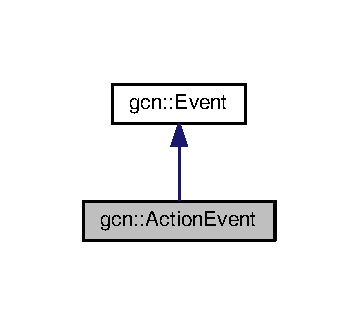
\includegraphics[width=172pt]{classgcn_1_1ActionEvent__inherit__graph}
\end{center}
\end{figure}


Collaboration diagram for gcn\+:\+:Action\+Event\+:\nopagebreak
\begin{figure}[H]
\begin{center}
\leavevmode
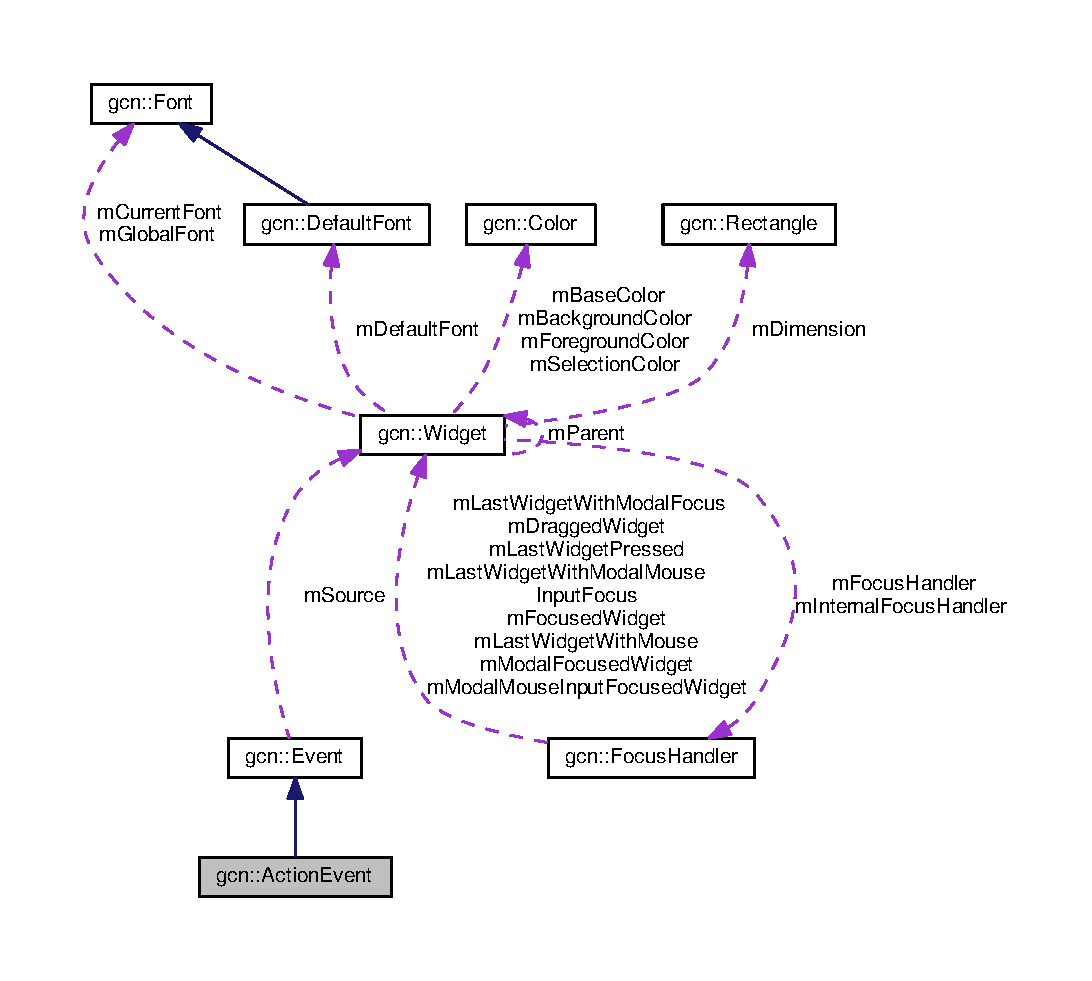
\includegraphics[width=350pt]{classgcn_1_1ActionEvent__coll__graph}
\end{center}
\end{figure}
\subsection*{Public Member Functions}
\begin{DoxyCompactItemize}
\item 
\hyperlink{classgcn_1_1ActionEvent_a7faee078e4958189de374050938a29d3}{Action\+Event} (\hyperlink{classgcn_1_1Widget}{Widget} $\ast$source, const std\+::string \&id)
\item 
virtual \hyperlink{classgcn_1_1ActionEvent_a9a87295a8d0d8897ddf49e3d53c522f0}{$\sim$\+Action\+Event} ()
\item 
const std\+::string \& \hyperlink{classgcn_1_1ActionEvent_a070935e55b7c64a8f1140dcba8d1391a}{get\+Id} () const 
\end{DoxyCompactItemize}
\subsection*{Protected Attributes}
\begin{DoxyCompactItemize}
\item 
std\+::string {\bfseries m\+Id}\hypertarget{classgcn_1_1ActionEvent_ac566911bc28a3d4f8dffbd82548f3e6e}{}\label{classgcn_1_1ActionEvent_ac566911bc28a3d4f8dffbd82548f3e6e}

\end{DoxyCompactItemize}


\subsection{Detailed Description}
Represents an action event.

\begin{DoxyAuthor}{Author}
Olof Naess�n 
\end{DoxyAuthor}
\begin{DoxySince}{Since}
0.\+6.\+0 
\end{DoxySince}


\subsection{Constructor \& Destructor Documentation}
\index{gcn\+::\+Action\+Event@{gcn\+::\+Action\+Event}!Action\+Event@{Action\+Event}}
\index{Action\+Event@{Action\+Event}!gcn\+::\+Action\+Event@{gcn\+::\+Action\+Event}}
\subsubsection[{\texorpdfstring{Action\+Event(\+Widget $\ast$source, const std\+::string \&id)}{ActionEvent(Widget *source, const std::string &id)}}]{\setlength{\rightskip}{0pt plus 5cm}gcn\+::\+Action\+Event\+::\+Action\+Event (
\begin{DoxyParamCaption}
\item[{{\bf Widget} $\ast$}]{source, }
\item[{const std\+::string \&}]{id}
\end{DoxyParamCaption}
)}\hypertarget{classgcn_1_1ActionEvent_a7faee078e4958189de374050938a29d3}{}\label{classgcn_1_1ActionEvent_a7faee078e4958189de374050938a29d3}
Constructor.


\begin{DoxyParams}{Parameters}
{\em source} & the source widget of the event. \\
\hline
{\em id} & the identifier of the event. \\
\hline
\end{DoxyParams}
\index{gcn\+::\+Action\+Event@{gcn\+::\+Action\+Event}!````~Action\+Event@{$\sim$\+Action\+Event}}
\index{````~Action\+Event@{$\sim$\+Action\+Event}!gcn\+::\+Action\+Event@{gcn\+::\+Action\+Event}}
\subsubsection[{\texorpdfstring{$\sim$\+Action\+Event()}{~ActionEvent()}}]{\setlength{\rightskip}{0pt plus 5cm}gcn\+::\+Action\+Event\+::$\sim$\+Action\+Event (
\begin{DoxyParamCaption}
{}
\end{DoxyParamCaption}
)\hspace{0.3cm}{\ttfamily [virtual]}}\hypertarget{classgcn_1_1ActionEvent_a9a87295a8d0d8897ddf49e3d53c522f0}{}\label{classgcn_1_1ActionEvent_a9a87295a8d0d8897ddf49e3d53c522f0}
Destructor. 

\subsection{Member Function Documentation}
\index{gcn\+::\+Action\+Event@{gcn\+::\+Action\+Event}!get\+Id@{get\+Id}}
\index{get\+Id@{get\+Id}!gcn\+::\+Action\+Event@{gcn\+::\+Action\+Event}}
\subsubsection[{\texorpdfstring{get\+Id() const }{getId() const }}]{\setlength{\rightskip}{0pt plus 5cm}const std\+::string \& gcn\+::\+Action\+Event\+::get\+Id (
\begin{DoxyParamCaption}
{}
\end{DoxyParamCaption}
) const}\hypertarget{classgcn_1_1ActionEvent_a070935e55b7c64a8f1140dcba8d1391a}{}\label{classgcn_1_1ActionEvent_a070935e55b7c64a8f1140dcba8d1391a}
Gets the id of the event.

\begin{DoxyReturn}{Returns}
the id of the event. 
\end{DoxyReturn}


The documentation for this class was generated from the following files\+:\begin{DoxyCompactItemize}
\item 
include/guisan/actionevent.\+hpp\item 
src/actionevent.\+cpp\end{DoxyCompactItemize}

\hypertarget{classgcn_1_1ActionListener}{}\section{gcn\+:\+:Action\+Listener Class Reference}
\label{classgcn_1_1ActionListener}\index{gcn\+::\+Action\+Listener@{gcn\+::\+Action\+Listener}}


{\ttfamily \#include $<$actionlistener.\+hpp$>$}



Inheritance diagram for gcn\+:\+:Action\+Listener\+:\nopagebreak
\begin{figure}[H]
\begin{center}
\leavevmode
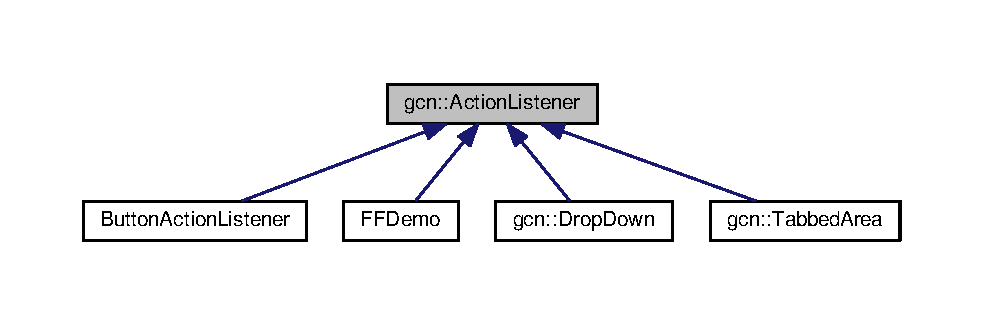
\includegraphics[width=350pt]{classgcn_1_1ActionListener__inherit__graph}
\end{center}
\end{figure}
\subsection*{Public Member Functions}
\begin{DoxyCompactItemize}
\item 
virtual \hyperlink{classgcn_1_1ActionListener_a15539005829890078792ce695260114b}{$\sim$\+Action\+Listener} ()
\item 
virtual void \hyperlink{classgcn_1_1ActionListener_ae883112ab054a8589b5d82c47763a31d}{action} (const \hyperlink{classgcn_1_1ActionEvent}{Action\+Event} \&action\+Event)=0
\end{DoxyCompactItemize}


\subsection{Detailed Description}
Listener of action events from Widgets. To be able to listen for actions you must make a class which inherits from this class and implements the action function.

\begin{DoxySeeAlso}{See also}
\hyperlink{classgcn_1_1Widget_a2782a478efbb087830884d9f2dc8b487}{Widget\+::add\+Action\+Listener} 
\end{DoxySeeAlso}
\begin{DoxyAuthor}{Author}
Olof Naess�n 

Per Larsson 
\end{DoxyAuthor}


\subsection{Constructor \& Destructor Documentation}
\index{gcn\+::\+Action\+Listener@{gcn\+::\+Action\+Listener}!````~Action\+Listener@{$\sim$\+Action\+Listener}}
\index{````~Action\+Listener@{$\sim$\+Action\+Listener}!gcn\+::\+Action\+Listener@{gcn\+::\+Action\+Listener}}
\subsubsection[{\texorpdfstring{$\sim$\+Action\+Listener()}{~ActionListener()}}]{\setlength{\rightskip}{0pt plus 5cm}virtual gcn\+::\+Action\+Listener\+::$\sim$\+Action\+Listener (
\begin{DoxyParamCaption}
{}
\end{DoxyParamCaption}
)\hspace{0.3cm}{\ttfamily [inline]}, {\ttfamily [virtual]}}\hypertarget{classgcn_1_1ActionListener_a15539005829890078792ce695260114b}{}\label{classgcn_1_1ActionListener_a15539005829890078792ce695260114b}
Destructor. 

\subsection{Member Function Documentation}
\index{gcn\+::\+Action\+Listener@{gcn\+::\+Action\+Listener}!action@{action}}
\index{action@{action}!gcn\+::\+Action\+Listener@{gcn\+::\+Action\+Listener}}
\subsubsection[{\texorpdfstring{action(const Action\+Event \&action\+Event)=0}{action(const ActionEvent &actionEvent)=0}}]{\setlength{\rightskip}{0pt plus 5cm}virtual void gcn\+::\+Action\+Listener\+::action (
\begin{DoxyParamCaption}
\item[{const {\bf Action\+Event} \&}]{action\+Event}
\end{DoxyParamCaption}
)\hspace{0.3cm}{\ttfamily [pure virtual]}}\hypertarget{classgcn_1_1ActionListener_ae883112ab054a8589b5d82c47763a31d}{}\label{classgcn_1_1ActionListener_ae883112ab054a8589b5d82c47763a31d}
Called when an action is recieved from a \hyperlink{classgcn_1_1Widget}{Widget}. It is used to be able to recieve a notification that an action has occured.


\begin{DoxyParams}{Parameters}
{\em action\+Event} & the event of the action. \\
\hline
\end{DoxyParams}
\begin{DoxySince}{Since}
0.\+6.\+0 
\end{DoxySince}


Implemented in \hyperlink{classgcn_1_1DropDown_aed63325d931d3d9d3df7400bd3b89f3e}{gcn\+::\+Drop\+Down}, \hyperlink{classgcn_1_1TabbedArea_ae9e032989a974cee2f2410779d6b95c3}{gcn\+::\+Tabbed\+Area}, \hyperlink{classFFDemo_ab7c02fe745edd2e4de4a9fd17b30abc2}{F\+F\+Demo}, and \hyperlink{classButtonActionListener_af6e587e3bdc21b68493b303af2753483}{Button\+Action\+Listener}.



The documentation for this class was generated from the following file\+:\begin{DoxyCompactItemize}
\item 
include/guisan/actionlistener.\+hpp\end{DoxyCompactItemize}

\hypertarget{classgcn_1_1BasicContainer}{}\section{gcn\+:\+:Basic\+Container Class Reference}
\label{classgcn_1_1BasicContainer}\index{gcn\+::\+Basic\+Container@{gcn\+::\+Basic\+Container}}


{\ttfamily \#include $<$basiccontainer.\+hpp$>$}



Inheritance diagram for gcn\+:\+:Basic\+Container\+:\nopagebreak
\begin{figure}[H]
\begin{center}
\leavevmode
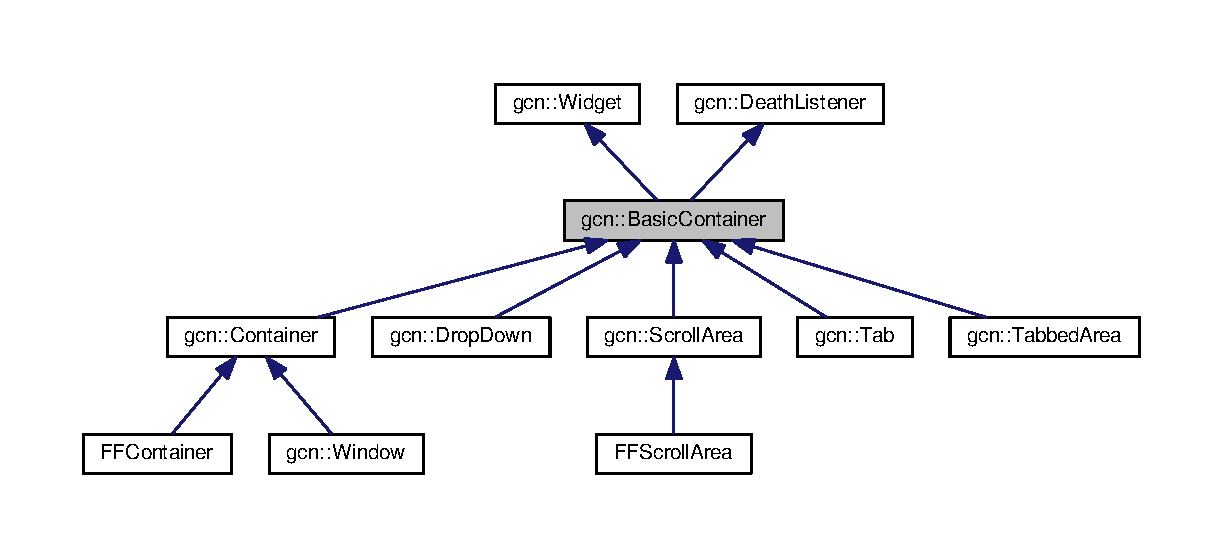
\includegraphics[width=350pt]{classgcn_1_1BasicContainer__inherit__graph}
\end{center}
\end{figure}


Collaboration diagram for gcn\+:\+:Basic\+Container\+:\nopagebreak
\begin{figure}[H]
\begin{center}
\leavevmode
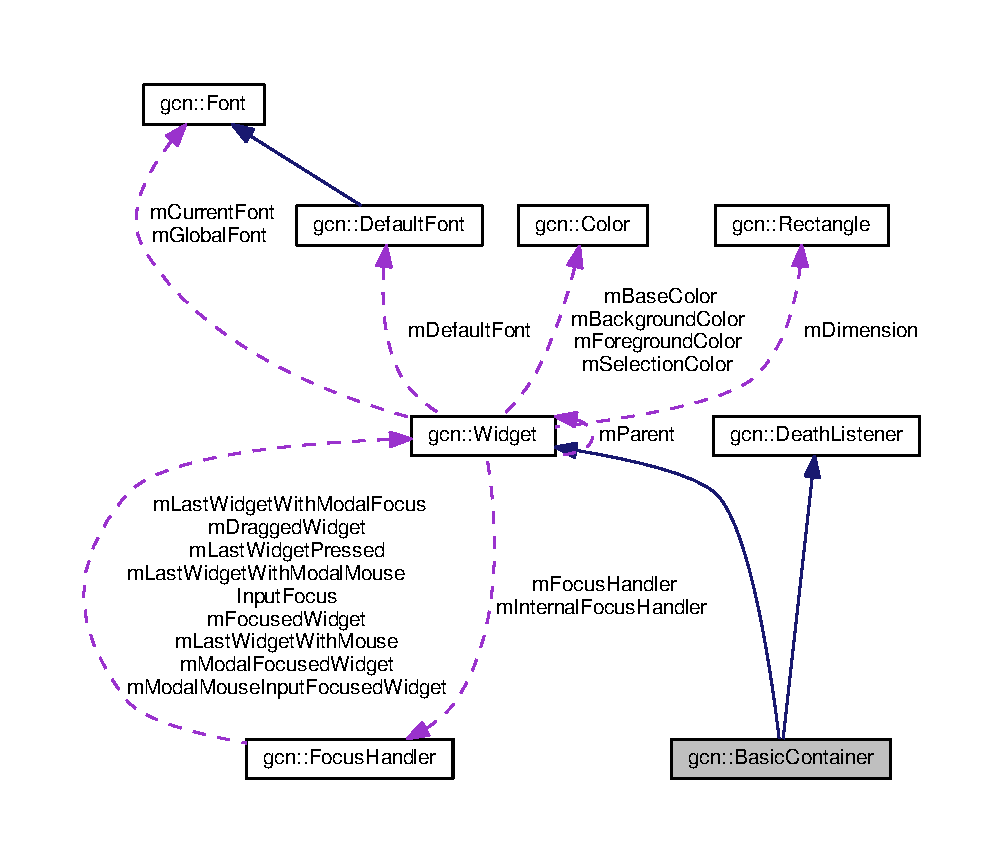
\includegraphics[width=350pt]{classgcn_1_1BasicContainer__coll__graph}
\end{center}
\end{figure}
\subsection*{Public Member Functions}
\begin{DoxyCompactItemize}
\item 
virtual \hyperlink{classgcn_1_1BasicContainer_ae70f53b73c7883b52105c714941c6052}{$\sim$\+Basic\+Container} ()
\item 
virtual void \hyperlink{classgcn_1_1BasicContainer_aa7b839a750b130894a3cc0c3fcbfa616}{move\+To\+Top} (\hyperlink{classgcn_1_1Widget}{Widget} $\ast$widget)
\item 
virtual void \hyperlink{classgcn_1_1BasicContainer_af1cd1b60207ccb0ae7263f8a34cce6b3}{move\+To\+Bottom} (\hyperlink{classgcn_1_1Widget}{Widget} $\ast$widget)
\item 
virtual \hyperlink{classgcn_1_1Rectangle}{Rectangle} \hyperlink{classgcn_1_1BasicContainer_a8ed853146d726cb3bc5d109ad52203d6}{get\+Children\+Area} ()
\item 
virtual void \hyperlink{classgcn_1_1BasicContainer_abc34133a4451f7ffce91ac4fcb7c63c9}{focus\+Next} ()
\item 
virtual void \hyperlink{classgcn_1_1BasicContainer_a480e30833f2d7af7283ea5c7ea4bb1b0}{focus\+Previous} ()
\item 
virtual void \hyperlink{classgcn_1_1BasicContainer_a65972968364c62bf244985b2900eaf25}{logic} ()
\item 
virtual void \hyperlink{classgcn_1_1BasicContainer_a90e4cc263111652a8c50d5395945bb65}{\+\_\+set\+Focus\+Handler} (\hyperlink{classgcn_1_1FocusHandler}{Focus\+Handler} $\ast$focus\+Handler)
\item 
void {\bfseries set\+Internal\+Focus\+Handler} (\hyperlink{classgcn_1_1FocusHandler}{Focus\+Handler} $\ast$focus\+Handler)\hypertarget{classgcn_1_1BasicContainer_a8d6ab7ef2f9a60d014783b712b9bca8f}{}\label{classgcn_1_1BasicContainer_a8d6ab7ef2f9a60d014783b712b9bca8f}

\item 
virtual void \hyperlink{classgcn_1_1BasicContainer_a5843702859ccb407f308cbe5d8987d28}{show\+Widget\+Part} (\hyperlink{classgcn_1_1Widget}{Widget} $\ast$widget, \hyperlink{classgcn_1_1Rectangle}{Rectangle} area)
\item 
virtual \hyperlink{classgcn_1_1Widget}{Widget} $\ast$ \hyperlink{classgcn_1_1BasicContainer_a99fd5e886776ec35d296c40755462a48}{get\+Widget\+At} (int x, int y)
\item 
virtual void \hyperlink{classgcn_1_1BasicContainer_ac6cf8760537dcd167e0f518f556bccf4}{death} (const \hyperlink{classgcn_1_1Event}{Event} \&event)
\end{DoxyCompactItemize}
\subsection*{Protected Types}
\begin{DoxyCompactItemize}
\item 
typedef std\+::list$<$ \hyperlink{classgcn_1_1Widget}{Widget} $\ast$ $>$ {\bfseries Widget\+List}\hypertarget{classgcn_1_1BasicContainer_a64f7237f6c610efba3e4928b09ee67d2}{}\label{classgcn_1_1BasicContainer_a64f7237f6c610efba3e4928b09ee67d2}

\item 
typedef Widget\+List\+::iterator {\bfseries Widget\+List\+Iterator}\hypertarget{classgcn_1_1BasicContainer_ad3791ca5ff8504602eaa0110d36f4822}{}\label{classgcn_1_1BasicContainer_ad3791ca5ff8504602eaa0110d36f4822}

\item 
typedef Widget\+List\+::reverse\+\_\+iterator {\bfseries Widget\+List\+Reverse\+Iterator}\hypertarget{classgcn_1_1BasicContainer_a6bda9a182a96ce1b7cad9e271c14cfb0}{}\label{classgcn_1_1BasicContainer_a6bda9a182a96ce1b7cad9e271c14cfb0}

\end{DoxyCompactItemize}
\subsection*{Protected Member Functions}
\begin{DoxyCompactItemize}
\item 
void \hyperlink{classgcn_1_1BasicContainer_a27d6058336a2573b6cea6e947c8d69bd}{add} (\hyperlink{classgcn_1_1Widget}{Widget} $\ast$widget)
\item 
virtual void \hyperlink{classgcn_1_1BasicContainer_a1e834058961f0cf6d1eea415ca509b10}{remove} (\hyperlink{classgcn_1_1Widget}{Widget} $\ast$widget)
\item 
virtual void \hyperlink{classgcn_1_1BasicContainer_a6b494b3e7c7369efcfc0e3f2f964bcf8}{clear} ()
\item 
virtual void \hyperlink{classgcn_1_1BasicContainer_a0e16996a51b1364875e9c48fe5c12bae}{draw\+Children} (\hyperlink{classgcn_1_1Graphics}{Graphics} $\ast$graphics)
\item 
virtual void \hyperlink{classgcn_1_1BasicContainer_a2d29dcdef360e36a3061aafccb407f28}{logic\+Children} ()
\item 
virtual \hyperlink{classgcn_1_1Widget}{Widget} $\ast$ \hyperlink{classgcn_1_1BasicContainer_a4c734912bb5342259dc7bd77d606bd7e}{find\+Widget\+By\+Id} (const std\+::string \&id)
\end{DoxyCompactItemize}
\subsection*{Protected Attributes}
\begin{DoxyCompactItemize}
\item 
Widget\+List {\bfseries m\+Widgets}\hypertarget{classgcn_1_1BasicContainer_a8729f791ac1ce256f8058ba32645cd25}{}\label{classgcn_1_1BasicContainer_a8729f791ac1ce256f8058ba32645cd25}

\end{DoxyCompactItemize}
\subsection*{Additional Inherited Members}


\subsection{Detailed Description}
Implements basic container behaviour. Most container will suffice by inheriting from this class.

\begin{DoxySeeAlso}{See also}
\hyperlink{classgcn_1_1Container}{Container} 
\end{DoxySeeAlso}


\subsection{Constructor \& Destructor Documentation}
\index{gcn\+::\+Basic\+Container@{gcn\+::\+Basic\+Container}!````~Basic\+Container@{$\sim$\+Basic\+Container}}
\index{````~Basic\+Container@{$\sim$\+Basic\+Container}!gcn\+::\+Basic\+Container@{gcn\+::\+Basic\+Container}}
\subsubsection[{\texorpdfstring{$\sim$\+Basic\+Container()}{~BasicContainer()}}]{\setlength{\rightskip}{0pt plus 5cm}gcn\+::\+Basic\+Container\+::$\sim$\+Basic\+Container (
\begin{DoxyParamCaption}
{}
\end{DoxyParamCaption}
)\hspace{0.3cm}{\ttfamily [virtual]}}\hypertarget{classgcn_1_1BasicContainer_ae70f53b73c7883b52105c714941c6052}{}\label{classgcn_1_1BasicContainer_ae70f53b73c7883b52105c714941c6052}
Destructor 

\subsection{Member Function Documentation}
\index{gcn\+::\+Basic\+Container@{gcn\+::\+Basic\+Container}!\+\_\+set\+Focus\+Handler@{\+\_\+set\+Focus\+Handler}}
\index{\+\_\+set\+Focus\+Handler@{\+\_\+set\+Focus\+Handler}!gcn\+::\+Basic\+Container@{gcn\+::\+Basic\+Container}}
\subsubsection[{\texorpdfstring{\+\_\+set\+Focus\+Handler(\+Focus\+Handler $\ast$focus\+Handler)}{_setFocusHandler(FocusHandler *focusHandler)}}]{\setlength{\rightskip}{0pt plus 5cm}void gcn\+::\+Basic\+Container\+::\+\_\+set\+Focus\+Handler (
\begin{DoxyParamCaption}
\item[{{\bf Focus\+Handler} $\ast$}]{focus\+Handler}
\end{DoxyParamCaption}
)\hspace{0.3cm}{\ttfamily [virtual]}}\hypertarget{classgcn_1_1BasicContainer_a90e4cc263111652a8c50d5395945bb65}{}\label{classgcn_1_1BasicContainer_a90e4cc263111652a8c50d5395945bb65}
Sets the \hyperlink{classgcn_1_1FocusHandler}{Focus\+Handler} to be used.

W\+A\+R\+N\+I\+NG\+: This function is used internally and should not be called or overloaded unless you know what you are doing.


\begin{DoxyParams}{Parameters}
{\em focus\+Handler} & the \hyperlink{classgcn_1_1FocusHandler}{Focus\+Handler} to use. \\
\hline
\end{DoxyParams}


Reimplemented from \hyperlink{classgcn_1_1Widget_a6c3ec01422e51978a643ddd3ae09c26a}{gcn\+::\+Widget}.

\index{gcn\+::\+Basic\+Container@{gcn\+::\+Basic\+Container}!add@{add}}
\index{add@{add}!gcn\+::\+Basic\+Container@{gcn\+::\+Basic\+Container}}
\subsubsection[{\texorpdfstring{add(\+Widget $\ast$widget)}{add(Widget *widget)}}]{\setlength{\rightskip}{0pt plus 5cm}void gcn\+::\+Basic\+Container\+::add (
\begin{DoxyParamCaption}
\item[{{\bf Widget} $\ast$}]{widget}
\end{DoxyParamCaption}
)\hspace{0.3cm}{\ttfamily [protected]}}\hypertarget{classgcn_1_1BasicContainer_a27d6058336a2573b6cea6e947c8d69bd}{}\label{classgcn_1_1BasicContainer_a27d6058336a2573b6cea6e947c8d69bd}
Adds a widget to the basic container.


\begin{DoxyParams}{Parameters}
{\em widget} & the widget to add. \\
\hline
\end{DoxyParams}
\index{gcn\+::\+Basic\+Container@{gcn\+::\+Basic\+Container}!clear@{clear}}
\index{clear@{clear}!gcn\+::\+Basic\+Container@{gcn\+::\+Basic\+Container}}
\subsubsection[{\texorpdfstring{clear()}{clear()}}]{\setlength{\rightskip}{0pt plus 5cm}void gcn\+::\+Basic\+Container\+::clear (
\begin{DoxyParamCaption}
{}
\end{DoxyParamCaption}
)\hspace{0.3cm}{\ttfamily [protected]}, {\ttfamily [virtual]}}\hypertarget{classgcn_1_1BasicContainer_a6b494b3e7c7369efcfc0e3f2f964bcf8}{}\label{classgcn_1_1BasicContainer_a6b494b3e7c7369efcfc0e3f2f964bcf8}
Clears the basic container from all widgets. 

Reimplemented in \hyperlink{classgcn_1_1Container_a561436ebcebc3419545a4db3397c6686}{gcn\+::\+Container}.

\index{gcn\+::\+Basic\+Container@{gcn\+::\+Basic\+Container}!death@{death}}
\index{death@{death}!gcn\+::\+Basic\+Container@{gcn\+::\+Basic\+Container}}
\subsubsection[{\texorpdfstring{death(const Event \&event)}{death(const Event &event)}}]{\setlength{\rightskip}{0pt plus 5cm}void gcn\+::\+Basic\+Container\+::death (
\begin{DoxyParamCaption}
\item[{const {\bf Event} \&}]{event}
\end{DoxyParamCaption}
)\hspace{0.3cm}{\ttfamily [virtual]}}\hypertarget{classgcn_1_1BasicContainer_ac6cf8760537dcd167e0f518f556bccf4}{}\label{classgcn_1_1BasicContainer_ac6cf8760537dcd167e0f518f556bccf4}
Called when a widget dies. It is used to be able to recieve a notification when a death of a widget occurs.


\begin{DoxyParams}{Parameters}
{\em event} & the event of the death. \\
\hline
\end{DoxyParams}


Implements \hyperlink{classgcn_1_1DeathListener_a526e786e21fcf1266a56f20617babf90}{gcn\+::\+Death\+Listener}.



Reimplemented in \hyperlink{classgcn_1_1DropDown_a8f6402e1ad3ac77b7db296bbd77a7494}{gcn\+::\+Drop\+Down}, and \hyperlink{classgcn_1_1TabbedArea_aacf206f5ea02e67b295b7b26ea2a6eac}{gcn\+::\+Tabbed\+Area}.

\index{gcn\+::\+Basic\+Container@{gcn\+::\+Basic\+Container}!draw\+Children@{draw\+Children}}
\index{draw\+Children@{draw\+Children}!gcn\+::\+Basic\+Container@{gcn\+::\+Basic\+Container}}
\subsubsection[{\texorpdfstring{draw\+Children(\+Graphics $\ast$graphics)}{drawChildren(Graphics *graphics)}}]{\setlength{\rightskip}{0pt plus 5cm}void gcn\+::\+Basic\+Container\+::draw\+Children (
\begin{DoxyParamCaption}
\item[{{\bf Graphics} $\ast$}]{graphics}
\end{DoxyParamCaption}
)\hspace{0.3cm}{\ttfamily [protected]}, {\ttfamily [virtual]}}\hypertarget{classgcn_1_1BasicContainer_a0e16996a51b1364875e9c48fe5c12bae}{}\label{classgcn_1_1BasicContainer_a0e16996a51b1364875e9c48fe5c12bae}
Draws children widgets.


\begin{DoxyParams}{Parameters}
{\em graphics} & a \hyperlink{classgcn_1_1Graphics}{Graphics} object to draw with. \\
\hline
\end{DoxyParams}
\index{gcn\+::\+Basic\+Container@{gcn\+::\+Basic\+Container}!find\+Widget\+By\+Id@{find\+Widget\+By\+Id}}
\index{find\+Widget\+By\+Id@{find\+Widget\+By\+Id}!gcn\+::\+Basic\+Container@{gcn\+::\+Basic\+Container}}
\subsubsection[{\texorpdfstring{find\+Widget\+By\+Id(const std\+::string \&id)}{findWidgetById(const std::string &id)}}]{\setlength{\rightskip}{0pt plus 5cm}{\bf Widget} $\ast$ gcn\+::\+Basic\+Container\+::find\+Widget\+By\+Id (
\begin{DoxyParamCaption}
\item[{const std\+::string \&}]{id}
\end{DoxyParamCaption}
)\hspace{0.3cm}{\ttfamily [protected]}, {\ttfamily [virtual]}}\hypertarget{classgcn_1_1BasicContainer_a4c734912bb5342259dc7bd77d606bd7e}{}\label{classgcn_1_1BasicContainer_a4c734912bb5342259dc7bd77d606bd7e}
Finds a widget given an id.


\begin{DoxyParams}{Parameters}
{\em id} & the id to find a widget by. \\
\hline
\end{DoxyParams}
\begin{DoxyReturn}{Returns}
the widget with the corrosponding id, N\+U\+LL of no widget is found. 
\end{DoxyReturn}


Reimplemented in \hyperlink{classgcn_1_1Container_a7871002a444dba6ad82df1dcef61561b}{gcn\+::\+Container}.

\index{gcn\+::\+Basic\+Container@{gcn\+::\+Basic\+Container}!focus\+Next@{focus\+Next}}
\index{focus\+Next@{focus\+Next}!gcn\+::\+Basic\+Container@{gcn\+::\+Basic\+Container}}
\subsubsection[{\texorpdfstring{focus\+Next()}{focusNext()}}]{\setlength{\rightskip}{0pt plus 5cm}void gcn\+::\+Basic\+Container\+::focus\+Next (
\begin{DoxyParamCaption}
{}
\end{DoxyParamCaption}
)\hspace{0.3cm}{\ttfamily [virtual]}}\hypertarget{classgcn_1_1BasicContainer_abc34133a4451f7ffce91ac4fcb7c63c9}{}\label{classgcn_1_1BasicContainer_abc34133a4451f7ffce91ac4fcb7c63c9}
Focuses the next widget in the widget. 

Reimplemented from \hyperlink{classgcn_1_1Widget_a4e76bde153710a1ee52ce100053c30b5}{gcn\+::\+Widget}.

\index{gcn\+::\+Basic\+Container@{gcn\+::\+Basic\+Container}!focus\+Previous@{focus\+Previous}}
\index{focus\+Previous@{focus\+Previous}!gcn\+::\+Basic\+Container@{gcn\+::\+Basic\+Container}}
\subsubsection[{\texorpdfstring{focus\+Previous()}{focusPrevious()}}]{\setlength{\rightskip}{0pt plus 5cm}void gcn\+::\+Basic\+Container\+::focus\+Previous (
\begin{DoxyParamCaption}
{}
\end{DoxyParamCaption}
)\hspace{0.3cm}{\ttfamily [virtual]}}\hypertarget{classgcn_1_1BasicContainer_a480e30833f2d7af7283ea5c7ea4bb1b0}{}\label{classgcn_1_1BasicContainer_a480e30833f2d7af7283ea5c7ea4bb1b0}
Focuses the previous widget in the widget. 

Reimplemented from \hyperlink{classgcn_1_1Widget_ae7a95f4088a5763f2004fe31fa12e363}{gcn\+::\+Widget}.

\index{gcn\+::\+Basic\+Container@{gcn\+::\+Basic\+Container}!get\+Children\+Area@{get\+Children\+Area}}
\index{get\+Children\+Area@{get\+Children\+Area}!gcn\+::\+Basic\+Container@{gcn\+::\+Basic\+Container}}
\subsubsection[{\texorpdfstring{get\+Children\+Area()}{getChildrenArea()}}]{\setlength{\rightskip}{0pt plus 5cm}{\bf Rectangle} gcn\+::\+Basic\+Container\+::get\+Children\+Area (
\begin{DoxyParamCaption}
{}
\end{DoxyParamCaption}
)\hspace{0.3cm}{\ttfamily [virtual]}}\hypertarget{classgcn_1_1BasicContainer_a8ed853146d726cb3bc5d109ad52203d6}{}\label{classgcn_1_1BasicContainer_a8ed853146d726cb3bc5d109ad52203d6}
Gets the subarea of the widget that the children occupy.

\begin{DoxyReturn}{Returns}
the subarea as a \hyperlink{classgcn_1_1Rectangle}{Rectangle}. 
\end{DoxyReturn}


Reimplemented from \hyperlink{classgcn_1_1Widget_a7bf115e02c4f14144e5bd57372850e41}{gcn\+::\+Widget}.



Reimplemented in \hyperlink{classgcn_1_1ScrollArea_a49333d5c588cf68aabe635f1cfd41543}{gcn\+::\+Scroll\+Area}, \hyperlink{classgcn_1_1DropDown_ad61f89e8985a3a3be217dd15e199633d}{gcn\+::\+Drop\+Down}, \hyperlink{classgcn_1_1Window_ae7022b52bb53543ff3cd366c124e15ff}{gcn\+::\+Window}, and \hyperlink{classFFContainer_af509106f3e9c8d69e821d864abfa1f7d}{F\+F\+Container}.

\index{gcn\+::\+Basic\+Container@{gcn\+::\+Basic\+Container}!get\+Widget\+At@{get\+Widget\+At}}
\index{get\+Widget\+At@{get\+Widget\+At}!gcn\+::\+Basic\+Container@{gcn\+::\+Basic\+Container}}
\subsubsection[{\texorpdfstring{get\+Widget\+At(int x, int y)}{getWidgetAt(int x, int y)}}]{\setlength{\rightskip}{0pt plus 5cm}{\bf Widget} $\ast$ gcn\+::\+Basic\+Container\+::get\+Widget\+At (
\begin{DoxyParamCaption}
\item[{int}]{x, }
\item[{int}]{y}
\end{DoxyParamCaption}
)\hspace{0.3cm}{\ttfamily [virtual]}}\hypertarget{classgcn_1_1BasicContainer_a99fd5e886776ec35d296c40755462a48}{}\label{classgcn_1_1BasicContainer_a99fd5e886776ec35d296c40755462a48}
Gets a widget from a certain position in the widget. This function is used to decide which gets mouse input, thus it can be overloaded to change that behaviour.

N\+O\+TE\+: This always returns N\+U\+LL if the widget is not a container.


\begin{DoxyParams}{Parameters}
{\em x} & the x coordinate. \\
\hline
{\em y} & the y coordinate. \\
\hline
\end{DoxyParams}
\begin{DoxyReturn}{Returns}
the widget at the specified coodinate, or N\+U\+LL if no such widget exists. 
\end{DoxyReturn}
\begin{DoxySince}{Since}
0.\+6.\+0 
\end{DoxySince}


Reimplemented from \hyperlink{classgcn_1_1Widget_aa5a319f7a99a02176be790a0ea92be92}{gcn\+::\+Widget}.



Reimplemented in \hyperlink{classgcn_1_1ScrollArea_afe0b59bef65e046032550dc76b5ba949}{gcn\+::\+Scroll\+Area}.

\index{gcn\+::\+Basic\+Container@{gcn\+::\+Basic\+Container}!logic@{logic}}
\index{logic@{logic}!gcn\+::\+Basic\+Container@{gcn\+::\+Basic\+Container}}
\subsubsection[{\texorpdfstring{logic()}{logic()}}]{\setlength{\rightskip}{0pt plus 5cm}void gcn\+::\+Basic\+Container\+::logic (
\begin{DoxyParamCaption}
{}
\end{DoxyParamCaption}
)\hspace{0.3cm}{\ttfamily [virtual]}}\hypertarget{classgcn_1_1BasicContainer_a65972968364c62bf244985b2900eaf25}{}\label{classgcn_1_1BasicContainer_a65972968364c62bf244985b2900eaf25}
Called for all widgets in the gui each time \hyperlink{classgcn_1_1Gui_a66744ebd628213d574bb6a7010781b1f}{Gui\+::logic} is called. You can do logic stuff here like playing an animation.

\begin{DoxySeeAlso}{See also}
\hyperlink{classgcn_1_1Gui}{Gui} 
\end{DoxySeeAlso}


Reimplemented from \hyperlink{classgcn_1_1Widget_aeb2e4c4751ef8666f48be1638ef8a48c}{gcn\+::\+Widget}.



Reimplemented in \hyperlink{classgcn_1_1ScrollArea_a7e9085abfccf6ebed42484226b4b2aeb}{gcn\+::\+Scroll\+Area}, \hyperlink{classgcn_1_1TabbedArea_a4adbdd819c9af603b20728d6e4cd5ce9}{gcn\+::\+Tabbed\+Area}, and \hyperlink{classFFContainer_a5d53541089f719665bfc2d689dab89c6}{F\+F\+Container}.

\index{gcn\+::\+Basic\+Container@{gcn\+::\+Basic\+Container}!logic\+Children@{logic\+Children}}
\index{logic\+Children@{logic\+Children}!gcn\+::\+Basic\+Container@{gcn\+::\+Basic\+Container}}
\subsubsection[{\texorpdfstring{logic\+Children()}{logicChildren()}}]{\setlength{\rightskip}{0pt plus 5cm}void gcn\+::\+Basic\+Container\+::logic\+Children (
\begin{DoxyParamCaption}
{}
\end{DoxyParamCaption}
)\hspace{0.3cm}{\ttfamily [protected]}, {\ttfamily [virtual]}}\hypertarget{classgcn_1_1BasicContainer_a2d29dcdef360e36a3061aafccb407f28}{}\label{classgcn_1_1BasicContainer_a2d29dcdef360e36a3061aafccb407f28}
Calls logic for children widgets. \index{gcn\+::\+Basic\+Container@{gcn\+::\+Basic\+Container}!move\+To\+Bottom@{move\+To\+Bottom}}
\index{move\+To\+Bottom@{move\+To\+Bottom}!gcn\+::\+Basic\+Container@{gcn\+::\+Basic\+Container}}
\subsubsection[{\texorpdfstring{move\+To\+Bottom(\+Widget $\ast$widget)}{moveToBottom(Widget *widget)}}]{\setlength{\rightskip}{0pt plus 5cm}void gcn\+::\+Basic\+Container\+::move\+To\+Bottom (
\begin{DoxyParamCaption}
\item[{{\bf Widget} $\ast$}]{widget}
\end{DoxyParamCaption}
)\hspace{0.3cm}{\ttfamily [virtual]}}\hypertarget{classgcn_1_1BasicContainer_af1cd1b60207ccb0ae7263f8a34cce6b3}{}\label{classgcn_1_1BasicContainer_af1cd1b60207ccb0ae7263f8a34cce6b3}
Moves a widget in this widget to the bottom of this widget. The moved widget will be drawn below all other widgets in this widget.


\begin{DoxyParams}{Parameters}
{\em widget} & the widget to move. \\
\hline
\end{DoxyParams}


Reimplemented from \hyperlink{classgcn_1_1Widget_a8e7a358c95db423ce9c4106d1985e875}{gcn\+::\+Widget}.

\index{gcn\+::\+Basic\+Container@{gcn\+::\+Basic\+Container}!move\+To\+Top@{move\+To\+Top}}
\index{move\+To\+Top@{move\+To\+Top}!gcn\+::\+Basic\+Container@{gcn\+::\+Basic\+Container}}
\subsubsection[{\texorpdfstring{move\+To\+Top(\+Widget $\ast$widget)}{moveToTop(Widget *widget)}}]{\setlength{\rightskip}{0pt plus 5cm}void gcn\+::\+Basic\+Container\+::move\+To\+Top (
\begin{DoxyParamCaption}
\item[{{\bf Widget} $\ast$}]{widget}
\end{DoxyParamCaption}
)\hspace{0.3cm}{\ttfamily [virtual]}}\hypertarget{classgcn_1_1BasicContainer_aa7b839a750b130894a3cc0c3fcbfa616}{}\label{classgcn_1_1BasicContainer_aa7b839a750b130894a3cc0c3fcbfa616}
Moves a widget to the top of this widget. The moved widget will be drawn above all other widgets in this widget.


\begin{DoxyParams}{Parameters}
{\em widget} & the widget to move. \\
\hline
\end{DoxyParams}


Reimplemented from \hyperlink{classgcn_1_1Widget_ad99dd66eb1b24911a73001f4bbdb1e39}{gcn\+::\+Widget}.

\index{gcn\+::\+Basic\+Container@{gcn\+::\+Basic\+Container}!remove@{remove}}
\index{remove@{remove}!gcn\+::\+Basic\+Container@{gcn\+::\+Basic\+Container}}
\subsubsection[{\texorpdfstring{remove(\+Widget $\ast$widget)}{remove(Widget *widget)}}]{\setlength{\rightskip}{0pt plus 5cm}void gcn\+::\+Basic\+Container\+::remove (
\begin{DoxyParamCaption}
\item[{{\bf Widget} $\ast$}]{widget}
\end{DoxyParamCaption}
)\hspace{0.3cm}{\ttfamily [protected]}, {\ttfamily [virtual]}}\hypertarget{classgcn_1_1BasicContainer_a1e834058961f0cf6d1eea415ca509b10}{}\label{classgcn_1_1BasicContainer_a1e834058961f0cf6d1eea415ca509b10}
Removes a widget from the basic container.


\begin{DoxyParams}{Parameters}
{\em widget} & the widget to remove. \\
\hline
\end{DoxyParams}


Reimplemented in \hyperlink{classgcn_1_1Container_a6ed5e946da5112c8b86d708c9000274e}{gcn\+::\+Container}.

\index{gcn\+::\+Basic\+Container@{gcn\+::\+Basic\+Container}!show\+Widget\+Part@{show\+Widget\+Part}}
\index{show\+Widget\+Part@{show\+Widget\+Part}!gcn\+::\+Basic\+Container@{gcn\+::\+Basic\+Container}}
\subsubsection[{\texorpdfstring{show\+Widget\+Part(\+Widget $\ast$widget, Rectangle area)}{showWidgetPart(Widget *widget, Rectangle area)}}]{\setlength{\rightskip}{0pt plus 5cm}void gcn\+::\+Basic\+Container\+::show\+Widget\+Part (
\begin{DoxyParamCaption}
\item[{{\bf Widget} $\ast$}]{widget, }
\item[{{\bf Rectangle}}]{area}
\end{DoxyParamCaption}
)\hspace{0.3cm}{\ttfamily [virtual]}}\hypertarget{classgcn_1_1BasicContainer_a5843702859ccb407f308cbe5d8987d28}{}\label{classgcn_1_1BasicContainer_a5843702859ccb407f308cbe5d8987d28}
Tries to show a specific part of a widget by moving it. Used if the widget should act as a container.


\begin{DoxyParams}{Parameters}
{\em widget} & the target widget. \\
\hline
{\em area} & the area to show. \\
\hline
\end{DoxyParams}


Reimplemented from \hyperlink{classgcn_1_1Widget_ad360f89bfa3c4de1c7919a01b99e9f28}{gcn\+::\+Widget}.



Reimplemented in \hyperlink{classgcn_1_1ScrollArea_a44138b1de2eb2b0b5c6366f573fd15e6}{gcn\+::\+Scroll\+Area}.



The documentation for this class was generated from the following files\+:\begin{DoxyCompactItemize}
\item 
include/guisan/basiccontainer.\+hpp\item 
src/basiccontainer.\+cpp\end{DoxyCompactItemize}

\hypertarget{classgcn_1_1Button}{}\section{gcn\+:\+:Button Class Reference}
\label{classgcn_1_1Button}\index{gcn\+::\+Button@{gcn\+::\+Button}}


{\ttfamily \#include $<$button.\+hpp$>$}



Inheritance diagram for gcn\+:\+:Button\+:\nopagebreak
\begin{figure}[H]
\begin{center}
\leavevmode
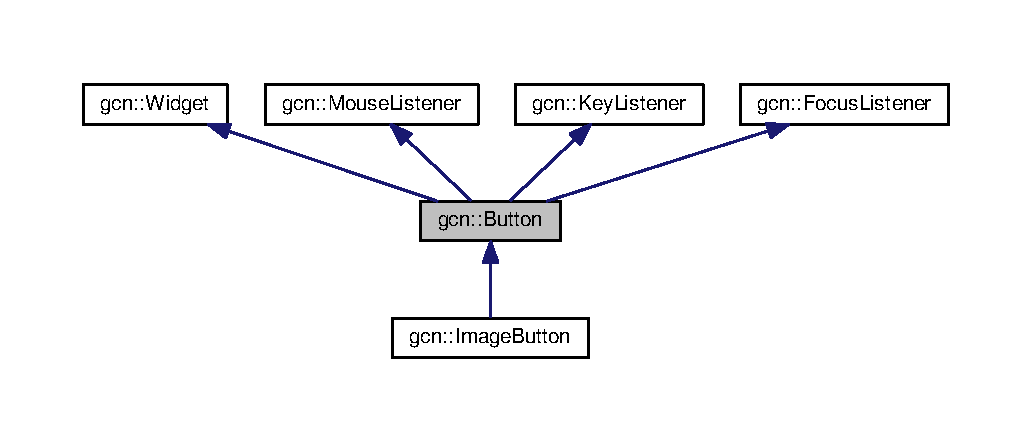
\includegraphics[width=350pt]{classgcn_1_1Button__inherit__graph}
\end{center}
\end{figure}


Collaboration diagram for gcn\+:\+:Button\+:\nopagebreak
\begin{figure}[H]
\begin{center}
\leavevmode
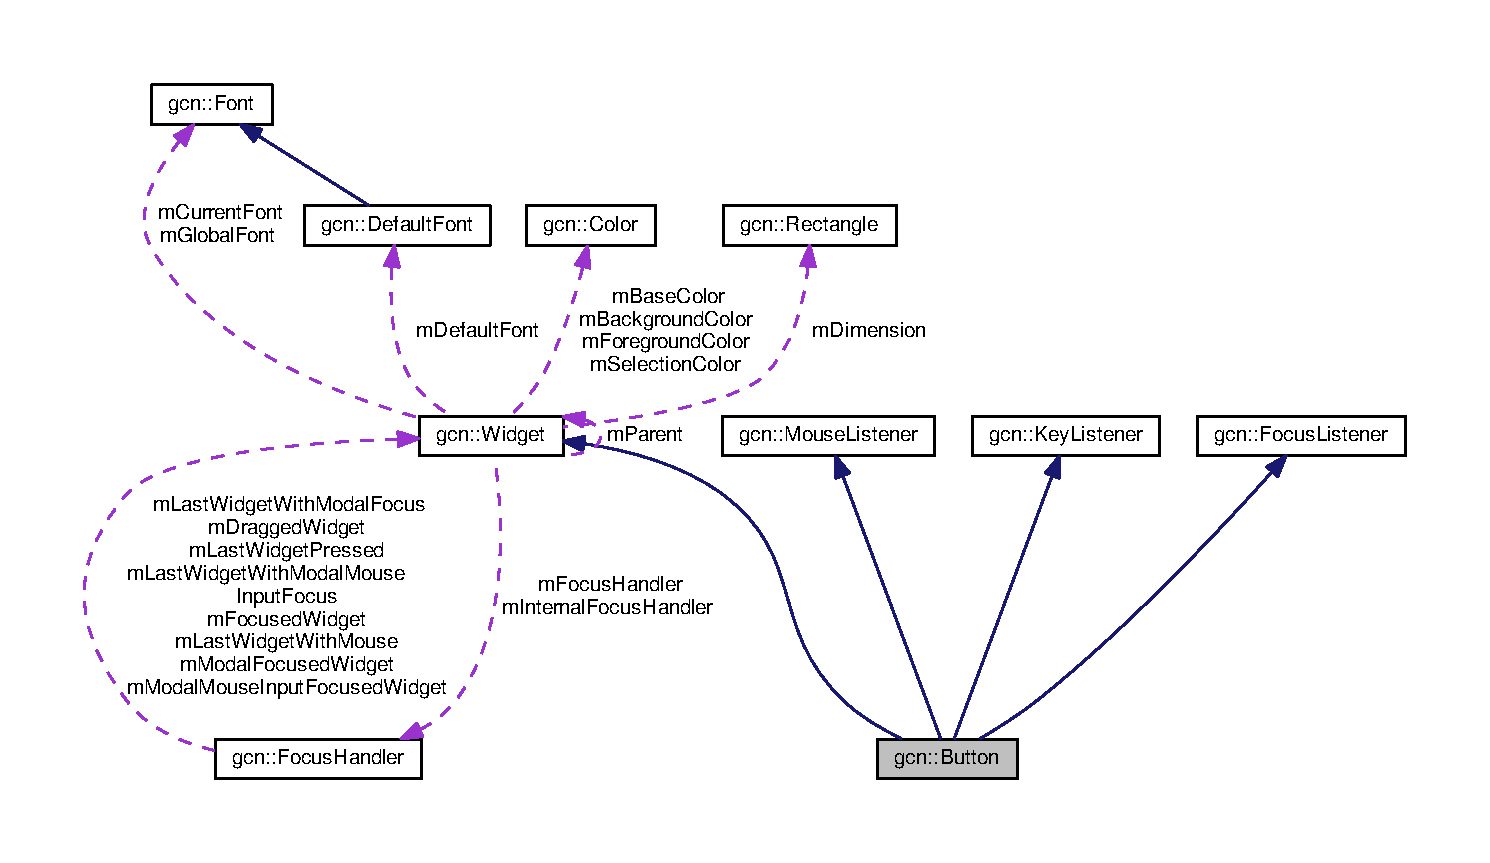
\includegraphics[width=350pt]{classgcn_1_1Button__coll__graph}
\end{center}
\end{figure}
\subsection*{Public Member Functions}
\begin{DoxyCompactItemize}
\item 
\hyperlink{classgcn_1_1Button_aaa7539ca928807770fcfa0ec8c028bb4}{Button} ()
\item 
\hyperlink{classgcn_1_1Button_aedec0a418abf43eca568a90e1e5b1e9c}{Button} (const std\+::string \&caption)
\item 
void \hyperlink{classgcn_1_1Button_a9f49ad1f0770a87a01fc77705f0b3a31}{set\+Caption} (const std\+::string \&caption)
\item 
const std\+::string \& \hyperlink{classgcn_1_1Button_a9d3be2d0f07d965feeabd0da7a6acf28}{get\+Caption} () const 
\item 
void \hyperlink{classgcn_1_1Button_a04bcbfda4c5fbd2781a78b126ea6f0ce}{set\+Alignment} (unsigned int alignment)
\item 
unsigned int \hyperlink{classgcn_1_1Button_aa8cbe52bc613600f60cb1cb292e3d56b}{get\+Alignment} () const 
\item 
void \hyperlink{classgcn_1_1Button_a2a04e95028ff614e90d9fbf0afb603e7}{set\+Spacing} (unsigned int spacing)
\item 
unsigned int \hyperlink{classgcn_1_1Button_a7a12a9dc96a30561c013099e648b612e}{get\+Spacing} () const 
\item 
void \hyperlink{classgcn_1_1Button_aea7387d84dd3ab70fb047c9c08a15ea2}{adjust\+Size} ()
\item 
bool \hyperlink{classgcn_1_1Button_a4a45119d1476b20834176ab8ffc95826}{is\+Pressed} () const 
\item 
virtual void \hyperlink{classgcn_1_1Button_a741dca35284e5155cd99c1e962e3d1e8}{draw} (\hyperlink{classgcn_1_1Graphics}{Graphics} $\ast$graphics)
\item 
virtual void \hyperlink{classgcn_1_1Button_a5d7f1dba36aa61524fb4c5b0ad47198b}{draw\+Border} (\hyperlink{classgcn_1_1Graphics}{Graphics} $\ast$graphics)
\item 
virtual void \hyperlink{classgcn_1_1Button_a6cee079024ffd4e8eeb8b682aade93c0}{focus\+Lost} (const \hyperlink{classgcn_1_1Event}{Event} \&event)
\item 
virtual void \hyperlink{classgcn_1_1Button_a7fe61128288965a4ec81d7e30cd3eba7}{mouse\+Pressed} (\hyperlink{classgcn_1_1MouseEvent}{Mouse\+Event} \&mouse\+Event)
\item 
virtual void \hyperlink{classgcn_1_1Button_abd8ca8cb9535bbce7e93006b792bf7dd}{mouse\+Released} (\hyperlink{classgcn_1_1MouseEvent}{Mouse\+Event} \&mouse\+Event)
\item 
virtual void \hyperlink{classgcn_1_1Button_a92a5874befc40b262207a21af20ba128}{mouse\+Entered} (\hyperlink{classgcn_1_1MouseEvent}{Mouse\+Event} \&mouse\+Event)
\item 
virtual void \hyperlink{classgcn_1_1Button_aeca3e20be574004eb22894d1d520a8e1}{mouse\+Exited} (\hyperlink{classgcn_1_1MouseEvent}{Mouse\+Event} \&mouse\+Event)
\item 
virtual void \hyperlink{classgcn_1_1Button_a2e938791d6c856d3b1835fc7a579690a}{mouse\+Dragged} (\hyperlink{classgcn_1_1MouseEvent}{Mouse\+Event} \&mouse\+Event)
\item 
virtual void \hyperlink{classgcn_1_1Button_a187855ce592e907e7b2e148ee4972c62}{key\+Pressed} (\hyperlink{classgcn_1_1KeyEvent}{Key\+Event} \&key\+Event)
\item 
virtual void \hyperlink{classgcn_1_1Button_a84a8355acfd340b6c0d189c6951fc8a5}{key\+Released} (\hyperlink{classgcn_1_1KeyEvent}{Key\+Event} \&key\+Event)
\end{DoxyCompactItemize}
\subsection*{Protected Attributes}
\begin{DoxyCompactItemize}
\item 
std\+::string {\bfseries m\+Caption}\hypertarget{classgcn_1_1Button_afa08738c837be849a98a375cfe09e8e1}{}\label{classgcn_1_1Button_afa08738c837be849a98a375cfe09e8e1}

\item 
bool {\bfseries m\+Has\+Mouse}\hypertarget{classgcn_1_1Button_a7533c90be7d71a4e3839b47f0463a787}{}\label{classgcn_1_1Button_a7533c90be7d71a4e3839b47f0463a787}

\item 
bool {\bfseries m\+Key\+Pressed}\hypertarget{classgcn_1_1Button_a54b4f3d1932a55d04b7e3c08857b529a}{}\label{classgcn_1_1Button_a54b4f3d1932a55d04b7e3c08857b529a}

\item 
bool {\bfseries m\+Mouse\+Pressed}\hypertarget{classgcn_1_1Button_a61abf0e4767c641923ad55fa869bbaae}{}\label{classgcn_1_1Button_a61abf0e4767c641923ad55fa869bbaae}

\item 
unsigned int {\bfseries m\+Alignment}\hypertarget{classgcn_1_1Button_ac31f520dfc7a3f72cf4f51c95ba4553f}{}\label{classgcn_1_1Button_ac31f520dfc7a3f72cf4f51c95ba4553f}

\item 
unsigned int {\bfseries m\+Spacing}\hypertarget{classgcn_1_1Button_a23c252a33155ea383334b564db7a9da5}{}\label{classgcn_1_1Button_a23c252a33155ea383334b564db7a9da5}

\end{DoxyCompactItemize}
\subsection*{Additional Inherited Members}


\subsection{Detailed Description}
A regular button. Add an \hyperlink{classgcn_1_1ActionListener}{Action\+Listener} to it to know when it has been clicked.

N\+O\+TE\+: You can only have text (a caption) on the button. If you want it to handle, for instance images, you can implement an \hyperlink{classgcn_1_1ImageButton}{Image\+Button} of your own and overload member functions from \hyperlink{classgcn_1_1Button}{Button}. 

\subsection{Constructor \& Destructor Documentation}
\index{gcn\+::\+Button@{gcn\+::\+Button}!Button@{Button}}
\index{Button@{Button}!gcn\+::\+Button@{gcn\+::\+Button}}
\subsubsection[{\texorpdfstring{Button()}{Button()}}]{\setlength{\rightskip}{0pt plus 5cm}gcn\+::\+Button\+::\+Button (
\begin{DoxyParamCaption}
{}
\end{DoxyParamCaption}
)}\hypertarget{classgcn_1_1Button_aaa7539ca928807770fcfa0ec8c028bb4}{}\label{classgcn_1_1Button_aaa7539ca928807770fcfa0ec8c028bb4}
Constructor. \index{gcn\+::\+Button@{gcn\+::\+Button}!Button@{Button}}
\index{Button@{Button}!gcn\+::\+Button@{gcn\+::\+Button}}
\subsubsection[{\texorpdfstring{Button(const std\+::string \&caption)}{Button(const std::string &caption)}}]{\setlength{\rightskip}{0pt plus 5cm}gcn\+::\+Button\+::\+Button (
\begin{DoxyParamCaption}
\item[{const std\+::string \&}]{caption}
\end{DoxyParamCaption}
)}\hypertarget{classgcn_1_1Button_aedec0a418abf43eca568a90e1e5b1e9c}{}\label{classgcn_1_1Button_aedec0a418abf43eca568a90e1e5b1e9c}
Constructor.


\begin{DoxyParams}{Parameters}
{\em caption} & the caption of the \hyperlink{classgcn_1_1Button}{Button}. \\
\hline
\end{DoxyParams}


\subsection{Member Function Documentation}
\index{gcn\+::\+Button@{gcn\+::\+Button}!adjust\+Size@{adjust\+Size}}
\index{adjust\+Size@{adjust\+Size}!gcn\+::\+Button@{gcn\+::\+Button}}
\subsubsection[{\texorpdfstring{adjust\+Size()}{adjustSize()}}]{\setlength{\rightskip}{0pt plus 5cm}void gcn\+::\+Button\+::adjust\+Size (
\begin{DoxyParamCaption}
{}
\end{DoxyParamCaption}
)}\hypertarget{classgcn_1_1Button_aea7387d84dd3ab70fb047c9c08a15ea2}{}\label{classgcn_1_1Button_aea7387d84dd3ab70fb047c9c08a15ea2}
Adjusts the buttons size to fit the content. \index{gcn\+::\+Button@{gcn\+::\+Button}!draw@{draw}}
\index{draw@{draw}!gcn\+::\+Button@{gcn\+::\+Button}}
\subsubsection[{\texorpdfstring{draw(\+Graphics $\ast$graphics)}{draw(Graphics *graphics)}}]{\setlength{\rightskip}{0pt plus 5cm}void gcn\+::\+Button\+::draw (
\begin{DoxyParamCaption}
\item[{{\bf Graphics} $\ast$}]{graphics}
\end{DoxyParamCaption}
)\hspace{0.3cm}{\ttfamily [virtual]}}\hypertarget{classgcn_1_1Button_a741dca35284e5155cd99c1e962e3d1e8}{}\label{classgcn_1_1Button_a741dca35284e5155cd99c1e962e3d1e8}
Draws the widget. It is called by the parent widget when it is time for the widget to draw itself. The graphics object is set up so that all drawing is relative to the widget, i.\+e coordinate (0,0) is the top-\/left corner of the widget. It is not possible to draw outside of a widgets dimension.


\begin{DoxyParams}{Parameters}
{\em graphics} & a \hyperlink{classgcn_1_1Graphics}{Graphics} object to draw with. \\
\hline
\end{DoxyParams}


Implements \hyperlink{classgcn_1_1Widget_acc595221d6a2d1afe1043c16dc37d212}{gcn\+::\+Widget}.



Reimplemented in \hyperlink{classgcn_1_1ImageButton_a067e502ef22fa2f443c575aca9cfe179}{gcn\+::\+Image\+Button}.

\index{gcn\+::\+Button@{gcn\+::\+Button}!draw\+Border@{draw\+Border}}
\index{draw\+Border@{draw\+Border}!gcn\+::\+Button@{gcn\+::\+Button}}
\subsubsection[{\texorpdfstring{draw\+Border(\+Graphics $\ast$graphics)}{drawBorder(Graphics *graphics)}}]{\setlength{\rightskip}{0pt plus 5cm}void gcn\+::\+Button\+::draw\+Border (
\begin{DoxyParamCaption}
\item[{{\bf Graphics} $\ast$}]{graphics}
\end{DoxyParamCaption}
)\hspace{0.3cm}{\ttfamily [virtual]}}\hypertarget{classgcn_1_1Button_a5d7f1dba36aa61524fb4c5b0ad47198b}{}\label{classgcn_1_1Button_a5d7f1dba36aa61524fb4c5b0ad47198b}
Draws the widget border. A border is drawn around a widget. The width and height of the border is therefore the widgets height+2$\ast$bordersize. Think of a painting that has a certain size, the border surrounds the painting.


\begin{DoxyParams}{Parameters}
{\em graphics} & a \hyperlink{classgcn_1_1Graphics}{Graphics} object to draw with. \\
\hline
\end{DoxyParams}


Reimplemented from \hyperlink{classgcn_1_1Widget_a58c3b2f513d8e029e321fd88a974f5c4}{gcn\+::\+Widget}.

\index{gcn\+::\+Button@{gcn\+::\+Button}!focus\+Lost@{focus\+Lost}}
\index{focus\+Lost@{focus\+Lost}!gcn\+::\+Button@{gcn\+::\+Button}}
\subsubsection[{\texorpdfstring{focus\+Lost(const Event \&event)}{focusLost(const Event &event)}}]{\setlength{\rightskip}{0pt plus 5cm}void gcn\+::\+Button\+::focus\+Lost (
\begin{DoxyParamCaption}
\item[{const {\bf Event} \&}]{event}
\end{DoxyParamCaption}
)\hspace{0.3cm}{\ttfamily [virtual]}}\hypertarget{classgcn_1_1Button_a6cee079024ffd4e8eeb8b682aade93c0}{}\label{classgcn_1_1Button_a6cee079024ffd4e8eeb8b682aade93c0}
Called when a widget loses focus.


\begin{DoxyParams}{Parameters}
{\em event} & discribes the event. \\
\hline
\end{DoxyParams}


Reimplemented from \hyperlink{classgcn_1_1FocusListener_a7523032b39888503179e8142d2433b45}{gcn\+::\+Focus\+Listener}.

\index{gcn\+::\+Button@{gcn\+::\+Button}!get\+Alignment@{get\+Alignment}}
\index{get\+Alignment@{get\+Alignment}!gcn\+::\+Button@{gcn\+::\+Button}}
\subsubsection[{\texorpdfstring{get\+Alignment() const }{getAlignment() const }}]{\setlength{\rightskip}{0pt plus 5cm}unsigned int gcn\+::\+Button\+::get\+Alignment (
\begin{DoxyParamCaption}
{}
\end{DoxyParamCaption}
) const}\hypertarget{classgcn_1_1Button_aa8cbe52bc613600f60cb1cb292e3d56b}{}\label{classgcn_1_1Button_aa8cbe52bc613600f60cb1cb292e3d56b}
Gets the alignment for the caption.

\begin{DoxyReturn}{Returns}
alignment of caption. 
\end{DoxyReturn}
\index{gcn\+::\+Button@{gcn\+::\+Button}!get\+Caption@{get\+Caption}}
\index{get\+Caption@{get\+Caption}!gcn\+::\+Button@{gcn\+::\+Button}}
\subsubsection[{\texorpdfstring{get\+Caption() const }{getCaption() const }}]{\setlength{\rightskip}{0pt plus 5cm}const std\+::string \& gcn\+::\+Button\+::get\+Caption (
\begin{DoxyParamCaption}
{}
\end{DoxyParamCaption}
) const}\hypertarget{classgcn_1_1Button_a9d3be2d0f07d965feeabd0da7a6acf28}{}\label{classgcn_1_1Button_a9d3be2d0f07d965feeabd0da7a6acf28}
Gets the \hyperlink{classgcn_1_1Button}{Button} caption.

\begin{DoxyReturn}{Returns}
the \hyperlink{classgcn_1_1Button}{Button} caption. 
\end{DoxyReturn}
\index{gcn\+::\+Button@{gcn\+::\+Button}!get\+Spacing@{get\+Spacing}}
\index{get\+Spacing@{get\+Spacing}!gcn\+::\+Button@{gcn\+::\+Button}}
\subsubsection[{\texorpdfstring{get\+Spacing() const }{getSpacing() const }}]{\setlength{\rightskip}{0pt plus 5cm}unsigned int gcn\+::\+Button\+::get\+Spacing (
\begin{DoxyParamCaption}
{}
\end{DoxyParamCaption}
) const}\hypertarget{classgcn_1_1Button_a7a12a9dc96a30561c013099e648b612e}{}\label{classgcn_1_1Button_a7a12a9dc96a30561c013099e648b612e}
Gets the spacing between the border of this button and its caption.

\begin{DoxyReturn}{Returns}
spacing. 
\end{DoxyReturn}
\index{gcn\+::\+Button@{gcn\+::\+Button}!is\+Pressed@{is\+Pressed}}
\index{is\+Pressed@{is\+Pressed}!gcn\+::\+Button@{gcn\+::\+Button}}
\subsubsection[{\texorpdfstring{is\+Pressed() const }{isPressed() const }}]{\setlength{\rightskip}{0pt plus 5cm}bool gcn\+::\+Button\+::is\+Pressed (
\begin{DoxyParamCaption}
{}
\end{DoxyParamCaption}
) const}\hypertarget{classgcn_1_1Button_a4a45119d1476b20834176ab8ffc95826}{}\label{classgcn_1_1Button_a4a45119d1476b20834176ab8ffc95826}
Checks if the button is pressed down. Useful when drawing.

\begin{DoxyReturn}{Returns}
true if the button is pressed down. 
\end{DoxyReturn}
\index{gcn\+::\+Button@{gcn\+::\+Button}!key\+Pressed@{key\+Pressed}}
\index{key\+Pressed@{key\+Pressed}!gcn\+::\+Button@{gcn\+::\+Button}}
\subsubsection[{\texorpdfstring{key\+Pressed(\+Key\+Event \&key\+Event)}{keyPressed(KeyEvent &keyEvent)}}]{\setlength{\rightskip}{0pt plus 5cm}void gcn\+::\+Button\+::key\+Pressed (
\begin{DoxyParamCaption}
\item[{{\bf Key\+Event} \&}]{key\+Event}
\end{DoxyParamCaption}
)\hspace{0.3cm}{\ttfamily [virtual]}}\hypertarget{classgcn_1_1Button_a187855ce592e907e7b2e148ee4972c62}{}\label{classgcn_1_1Button_a187855ce592e907e7b2e148ee4972c62}
Called if a key is pressed when the widget has keyboard focus. If a key is held down the widget will generate multiple key presses.


\begin{DoxyParams}{Parameters}
{\em key\+Event} & discribes the event. \\
\hline
\end{DoxyParams}


Reimplemented from \hyperlink{classgcn_1_1KeyListener_ada6c0d038340d6ee674702268b2d2c67}{gcn\+::\+Key\+Listener}.

\index{gcn\+::\+Button@{gcn\+::\+Button}!key\+Released@{key\+Released}}
\index{key\+Released@{key\+Released}!gcn\+::\+Button@{gcn\+::\+Button}}
\subsubsection[{\texorpdfstring{key\+Released(\+Key\+Event \&key\+Event)}{keyReleased(KeyEvent &keyEvent)}}]{\setlength{\rightskip}{0pt plus 5cm}void gcn\+::\+Button\+::key\+Released (
\begin{DoxyParamCaption}
\item[{{\bf Key\+Event} \&}]{key\+Event}
\end{DoxyParamCaption}
)\hspace{0.3cm}{\ttfamily [virtual]}}\hypertarget{classgcn_1_1Button_a84a8355acfd340b6c0d189c6951fc8a5}{}\label{classgcn_1_1Button_a84a8355acfd340b6c0d189c6951fc8a5}
Called if a key is released when the widget has keyboard focus.


\begin{DoxyParams}{Parameters}
{\em key\+Event} & discribes the event. \\
\hline
\end{DoxyParams}


Reimplemented from \hyperlink{classgcn_1_1KeyListener_a5cae3889ae71c19d3969b3b35bdf7f2e}{gcn\+::\+Key\+Listener}.

\index{gcn\+::\+Button@{gcn\+::\+Button}!mouse\+Dragged@{mouse\+Dragged}}
\index{mouse\+Dragged@{mouse\+Dragged}!gcn\+::\+Button@{gcn\+::\+Button}}
\subsubsection[{\texorpdfstring{mouse\+Dragged(\+Mouse\+Event \&mouse\+Event)}{mouseDragged(MouseEvent &mouseEvent)}}]{\setlength{\rightskip}{0pt plus 5cm}void gcn\+::\+Button\+::mouse\+Dragged (
\begin{DoxyParamCaption}
\item[{{\bf Mouse\+Event} \&}]{mouse\+Event}
\end{DoxyParamCaption}
)\hspace{0.3cm}{\ttfamily [virtual]}}\hypertarget{classgcn_1_1Button_a2e938791d6c856d3b1835fc7a579690a}{}\label{classgcn_1_1Button_a2e938791d6c856d3b1835fc7a579690a}
Called when the mouse has moved and the mouse has previously been pressed on the widget.


\begin{DoxyParams}{Parameters}
{\em mouse\+Event} & describes the event. \\
\hline
\end{DoxyParams}
\begin{DoxySince}{Since}
0.\+6.\+0 
\end{DoxySince}


Reimplemented from \hyperlink{classgcn_1_1MouseListener_a5e2764977dd75e52d116f9ba6311a46b}{gcn\+::\+Mouse\+Listener}.

\index{gcn\+::\+Button@{gcn\+::\+Button}!mouse\+Entered@{mouse\+Entered}}
\index{mouse\+Entered@{mouse\+Entered}!gcn\+::\+Button@{gcn\+::\+Button}}
\subsubsection[{\texorpdfstring{mouse\+Entered(\+Mouse\+Event \&mouse\+Event)}{mouseEntered(MouseEvent &mouseEvent)}}]{\setlength{\rightskip}{0pt plus 5cm}void gcn\+::\+Button\+::mouse\+Entered (
\begin{DoxyParamCaption}
\item[{{\bf Mouse\+Event} \&}]{mouse\+Event}
\end{DoxyParamCaption}
)\hspace{0.3cm}{\ttfamily [virtual]}}\hypertarget{classgcn_1_1Button_a92a5874befc40b262207a21af20ba128}{}\label{classgcn_1_1Button_a92a5874befc40b262207a21af20ba128}
Called when the mouse has entered into the widget area.


\begin{DoxyParams}{Parameters}
{\em mouse\+Event} & describes the event. \\
\hline
\end{DoxyParams}
\begin{DoxySince}{Since}
0.\+6.\+0 
\end{DoxySince}


Reimplemented from \hyperlink{classgcn_1_1MouseListener_a5d0fc52c1fd750eb76560fbc27672dac}{gcn\+::\+Mouse\+Listener}.

\index{gcn\+::\+Button@{gcn\+::\+Button}!mouse\+Exited@{mouse\+Exited}}
\index{mouse\+Exited@{mouse\+Exited}!gcn\+::\+Button@{gcn\+::\+Button}}
\subsubsection[{\texorpdfstring{mouse\+Exited(\+Mouse\+Event \&mouse\+Event)}{mouseExited(MouseEvent &mouseEvent)}}]{\setlength{\rightskip}{0pt plus 5cm}void gcn\+::\+Button\+::mouse\+Exited (
\begin{DoxyParamCaption}
\item[{{\bf Mouse\+Event} \&}]{mouse\+Event}
\end{DoxyParamCaption}
)\hspace{0.3cm}{\ttfamily [virtual]}}\hypertarget{classgcn_1_1Button_aeca3e20be574004eb22894d1d520a8e1}{}\label{classgcn_1_1Button_aeca3e20be574004eb22894d1d520a8e1}
Called when the mouse has exited the widget area.


\begin{DoxyParams}{Parameters}
{\em mouse\+Event} & describes the event. \\
\hline
\end{DoxyParams}


Reimplemented from \hyperlink{classgcn_1_1MouseListener_ac84dd820bbcf3bf9268776db69cbf114}{gcn\+::\+Mouse\+Listener}.

\index{gcn\+::\+Button@{gcn\+::\+Button}!mouse\+Pressed@{mouse\+Pressed}}
\index{mouse\+Pressed@{mouse\+Pressed}!gcn\+::\+Button@{gcn\+::\+Button}}
\subsubsection[{\texorpdfstring{mouse\+Pressed(\+Mouse\+Event \&mouse\+Event)}{mousePressed(MouseEvent &mouseEvent)}}]{\setlength{\rightskip}{0pt plus 5cm}void gcn\+::\+Button\+::mouse\+Pressed (
\begin{DoxyParamCaption}
\item[{{\bf Mouse\+Event} \&}]{mouse\+Event}
\end{DoxyParamCaption}
)\hspace{0.3cm}{\ttfamily [virtual]}}\hypertarget{classgcn_1_1Button_a7fe61128288965a4ec81d7e30cd3eba7}{}\label{classgcn_1_1Button_a7fe61128288965a4ec81d7e30cd3eba7}
Called when a mouse button has been pressed on the widget area.

N\+O\+TE\+: A mouse press is N\+OT equal to a mouse click. Use mouse\+Click\+Message to check for mouse clicks.


\begin{DoxyParams}{Parameters}
{\em mouse\+Event} & describes the event. \\
\hline
\end{DoxyParams}
\begin{DoxySince}{Since}
0.\+6.\+0 
\end{DoxySince}


Reimplemented from \hyperlink{classgcn_1_1MouseListener_af81ee6190a48a18585f6e738e381abd3}{gcn\+::\+Mouse\+Listener}.

\index{gcn\+::\+Button@{gcn\+::\+Button}!mouse\+Released@{mouse\+Released}}
\index{mouse\+Released@{mouse\+Released}!gcn\+::\+Button@{gcn\+::\+Button}}
\subsubsection[{\texorpdfstring{mouse\+Released(\+Mouse\+Event \&mouse\+Event)}{mouseReleased(MouseEvent &mouseEvent)}}]{\setlength{\rightskip}{0pt plus 5cm}void gcn\+::\+Button\+::mouse\+Released (
\begin{DoxyParamCaption}
\item[{{\bf Mouse\+Event} \&}]{mouse\+Event}
\end{DoxyParamCaption}
)\hspace{0.3cm}{\ttfamily [virtual]}}\hypertarget{classgcn_1_1Button_abd8ca8cb9535bbce7e93006b792bf7dd}{}\label{classgcn_1_1Button_abd8ca8cb9535bbce7e93006b792bf7dd}
Called when a mouse button has been released on the widget area.


\begin{DoxyParams}{Parameters}
{\em mouse\+Event} & describes the event. \\
\hline
\end{DoxyParams}


Reimplemented from \hyperlink{classgcn_1_1MouseListener_adf68ed80e1a3c027fbb5d0e575b20fc3}{gcn\+::\+Mouse\+Listener}.

\index{gcn\+::\+Button@{gcn\+::\+Button}!set\+Alignment@{set\+Alignment}}
\index{set\+Alignment@{set\+Alignment}!gcn\+::\+Button@{gcn\+::\+Button}}
\subsubsection[{\texorpdfstring{set\+Alignment(unsigned int alignment)}{setAlignment(unsigned int alignment)}}]{\setlength{\rightskip}{0pt plus 5cm}void gcn\+::\+Button\+::set\+Alignment (
\begin{DoxyParamCaption}
\item[{unsigned int}]{alignment}
\end{DoxyParamCaption}
)}\hypertarget{classgcn_1_1Button_a04bcbfda4c5fbd2781a78b126ea6f0ce}{}\label{classgcn_1_1Button_a04bcbfda4c5fbd2781a78b126ea6f0ce}
Sets the alignment for the caption.


\begin{DoxyParams}{Parameters}
{\em alignment} & Graphics\+::\+L\+E\+FT, Graphics\+::\+C\+E\+N\+T\+ER or Graphics\+::\+R\+I\+G\+HT \\
\hline
\end{DoxyParams}
\begin{DoxySeeAlso}{See also}
\hyperlink{classgcn_1_1Graphics}{Graphics} 
\end{DoxySeeAlso}
\index{gcn\+::\+Button@{gcn\+::\+Button}!set\+Caption@{set\+Caption}}
\index{set\+Caption@{set\+Caption}!gcn\+::\+Button@{gcn\+::\+Button}}
\subsubsection[{\texorpdfstring{set\+Caption(const std\+::string \&caption)}{setCaption(const std::string &caption)}}]{\setlength{\rightskip}{0pt plus 5cm}void gcn\+::\+Button\+::set\+Caption (
\begin{DoxyParamCaption}
\item[{const std\+::string \&}]{caption}
\end{DoxyParamCaption}
)}\hypertarget{classgcn_1_1Button_a9f49ad1f0770a87a01fc77705f0b3a31}{}\label{classgcn_1_1Button_a9f49ad1f0770a87a01fc77705f0b3a31}
Sets the \hyperlink{classgcn_1_1Button}{Button} caption.


\begin{DoxyParams}{Parameters}
{\em caption} & the \hyperlink{classgcn_1_1Button}{Button} caption. \\
\hline
\end{DoxyParams}
\index{gcn\+::\+Button@{gcn\+::\+Button}!set\+Spacing@{set\+Spacing}}
\index{set\+Spacing@{set\+Spacing}!gcn\+::\+Button@{gcn\+::\+Button}}
\subsubsection[{\texorpdfstring{set\+Spacing(unsigned int spacing)}{setSpacing(unsigned int spacing)}}]{\setlength{\rightskip}{0pt plus 5cm}void gcn\+::\+Button\+::set\+Spacing (
\begin{DoxyParamCaption}
\item[{unsigned int}]{spacing}
\end{DoxyParamCaption}
)}\hypertarget{classgcn_1_1Button_a2a04e95028ff614e90d9fbf0afb603e7}{}\label{classgcn_1_1Button_a2a04e95028ff614e90d9fbf0afb603e7}
Sets the spacing between the border of this button and its caption.


\begin{DoxyParams}{Parameters}
{\em spacing} & is a number between 0 and 255. The default value for spacing is 4 and can be changed using this method. \\
\hline
\end{DoxyParams}


The documentation for this class was generated from the following files\+:\begin{DoxyCompactItemize}
\item 
include/guisan/widgets/button.\+hpp\item 
src/widgets/button.\+cpp\end{DoxyCompactItemize}

\hypertarget{classButtonActionListener}{}\section{Button\+Action\+Listener Class Reference}
\label{classButtonActionListener}\index{Button\+Action\+Listener@{Button\+Action\+Listener}}


Inheritance diagram for Button\+Action\+Listener\+:\nopagebreak
\begin{figure}[H]
\begin{center}
\leavevmode
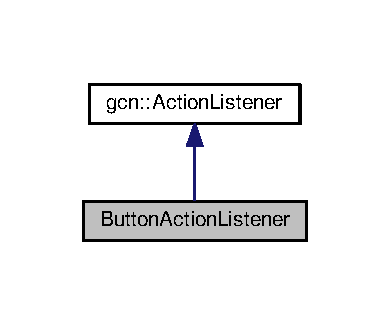
\includegraphics[width=187pt]{classButtonActionListener__inherit__graph}
\end{center}
\end{figure}


Collaboration diagram for Button\+Action\+Listener\+:\nopagebreak
\begin{figure}[H]
\begin{center}
\leavevmode
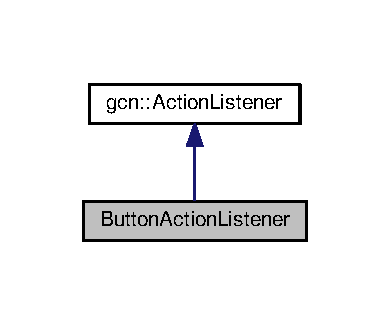
\includegraphics[width=187pt]{classButtonActionListener__coll__graph}
\end{center}
\end{figure}
\subsection*{Public Member Functions}
\begin{DoxyCompactItemize}
\item 
void \hyperlink{classButtonActionListener_af6e587e3bdc21b68493b303af2753483}{action} (const \hyperlink{classgcn_1_1ActionEvent}{gcn\+::\+Action\+Event} \&action\+Event)
\end{DoxyCompactItemize}


\subsection{Member Function Documentation}
\index{Button\+Action\+Listener@{Button\+Action\+Listener}!action@{action}}
\index{action@{action}!Button\+Action\+Listener@{Button\+Action\+Listener}}
\subsubsection[{\texorpdfstring{action(const gcn\+::\+Action\+Event \&action\+Event)}{action(const gcn::ActionEvent &actionEvent)}}]{\setlength{\rightskip}{0pt plus 5cm}void Button\+Action\+Listener\+::action (
\begin{DoxyParamCaption}
\item[{const {\bf gcn\+::\+Action\+Event} \&}]{action\+Event}
\end{DoxyParamCaption}
)\hspace{0.3cm}{\ttfamily [inline]}, {\ttfamily [virtual]}}\hypertarget{classButtonActionListener_af6e587e3bdc21b68493b303af2753483}{}\label{classButtonActionListener_af6e587e3bdc21b68493b303af2753483}
Called when an action is recieved from a Widget. It is used to be able to recieve a notification that an action has occured.


\begin{DoxyParams}{Parameters}
{\em action\+Event} & the event of the action. \\
\hline
\end{DoxyParams}
\begin{DoxySince}{Since}
0.\+6.\+0 
\end{DoxySince}


Implements \hyperlink{classgcn_1_1ActionListener_ae883112ab054a8589b5d82c47763a31d}{gcn\+::\+Action\+Listener}.



The documentation for this class was generated from the following file\+:\begin{DoxyCompactItemize}
\item 
examples/sdlaction.\+cpp\end{DoxyCompactItemize}

\hypertarget{classgcn_1_1CheckBox}{}\section{gcn\+:\+:Check\+Box Class Reference}
\label{classgcn_1_1CheckBox}\index{gcn\+::\+Check\+Box@{gcn\+::\+Check\+Box}}


{\ttfamily \#include $<$checkbox.\+hpp$>$}



Inheritance diagram for gcn\+:\+:Check\+Box\+:\nopagebreak
\begin{figure}[H]
\begin{center}
\leavevmode
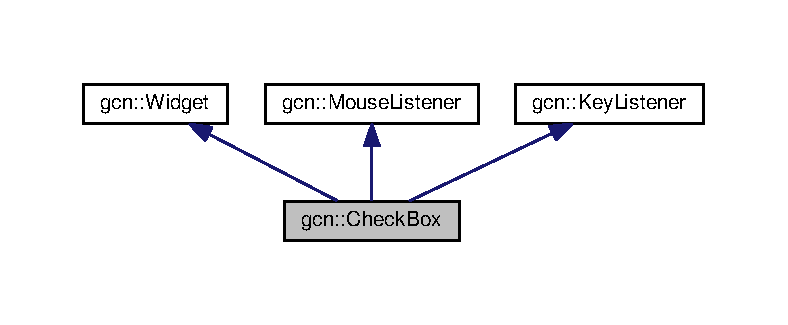
\includegraphics[width=350pt]{classgcn_1_1CheckBox__inherit__graph}
\end{center}
\end{figure}


Collaboration diagram for gcn\+:\+:Check\+Box\+:\nopagebreak
\begin{figure}[H]
\begin{center}
\leavevmode
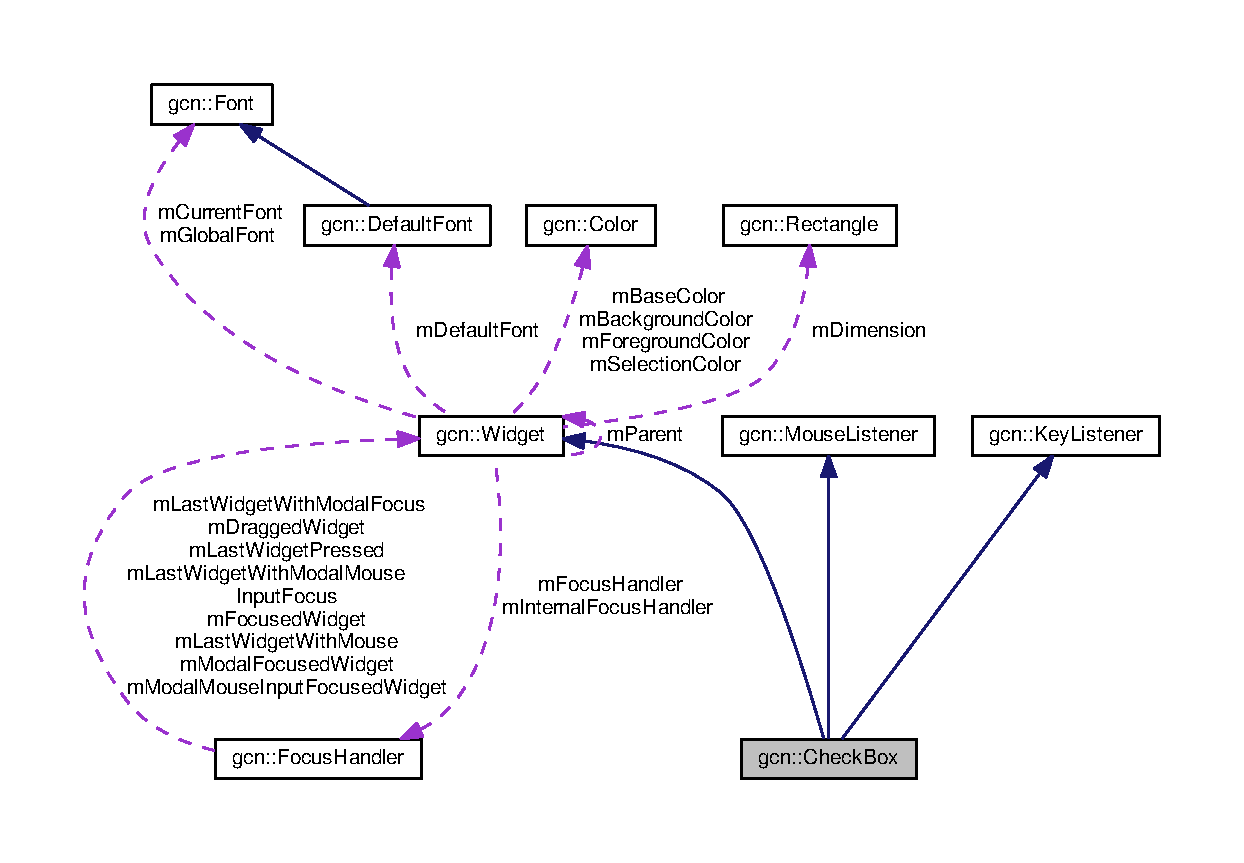
\includegraphics[width=350pt]{classgcn_1_1CheckBox__coll__graph}
\end{center}
\end{figure}
\subsection*{Public Member Functions}
\begin{DoxyCompactItemize}
\item 
\hyperlink{classgcn_1_1CheckBox_a0e81d7b6fd1e6b0d196c8d800a8e2610}{Check\+Box} ()
\item 
\hyperlink{classgcn_1_1CheckBox_aab17607081d115e303b847b0e57338ec}{Check\+Box} (const std\+::string \&caption, bool selected=false)
\item 
virtual \hyperlink{classgcn_1_1CheckBox_aec8d239efd70e47dcb4fdf7684d747e3}{$\sim$\+Check\+Box} ()
\item 
bool \hyperlink{classgcn_1_1CheckBox_aa50cd949abb713529eb8fa60d85ead45}{is\+Selected} () const 
\item 
void \hyperlink{classgcn_1_1CheckBox_afc33cf5fe07bd1c121f76ecc2a6f0729}{set\+Selected} (bool selected)
\item 
const std\+::string \& \hyperlink{classgcn_1_1CheckBox_ae8fa88932da62ef67d0d4f6b39bbaf15}{get\+Caption} () const 
\item 
void \hyperlink{classgcn_1_1CheckBox_a155f63ad8ffcf2f8200c3ffef274247d}{set\+Caption} (const std\+::string \&caption)
\item 
void \hyperlink{classgcn_1_1CheckBox_a18dd39feee57e6bfcef69fc9f5b00d08}{adjust\+Size} ()
\item 
virtual void \hyperlink{classgcn_1_1CheckBox_acd76dee289dcd7cc07ade85ce74c7d7c}{draw} (\hyperlink{classgcn_1_1Graphics}{Graphics} $\ast$graphics)
\item 
virtual void \hyperlink{classgcn_1_1CheckBox_a385eb0b9601f128646dc28b0e34c0293}{draw\+Border} (\hyperlink{classgcn_1_1Graphics}{Graphics} $\ast$graphics)
\item 
virtual void \hyperlink{classgcn_1_1CheckBox_a40a70ca664f54dd568b3522e6fb6e7ce}{key\+Pressed} (\hyperlink{classgcn_1_1KeyEvent}{Key\+Event} \&key\+Event)
\item 
virtual void \hyperlink{classgcn_1_1CheckBox_a968db12a9f01c70979ca06a179e8d565}{mouse\+Clicked} (\hyperlink{classgcn_1_1MouseEvent}{Mouse\+Event} \&mouse\+Event)
\item 
virtual void \hyperlink{classgcn_1_1CheckBox_adedbb4f9840c41a9e6943d2757986dff}{mouse\+Dragged} (\hyperlink{classgcn_1_1MouseEvent}{Mouse\+Event} \&mouse\+Event)
\end{DoxyCompactItemize}
\subsection*{Protected Member Functions}
\begin{DoxyCompactItemize}
\item 
virtual void \hyperlink{classgcn_1_1CheckBox_ab2aad0c0ee5a68d446aeb582143fac01}{draw\+Box} (\hyperlink{classgcn_1_1Graphics}{Graphics} $\ast$graphics)
\item 
virtual void \hyperlink{classgcn_1_1CheckBox_a65e7e1e0c924a2dc249131f7961aaeba}{toggle\+Selected} ()
\end{DoxyCompactItemize}
\subsection*{Protected Attributes}
\begin{DoxyCompactItemize}
\item 
bool \hyperlink{classgcn_1_1CheckBox_a2d0b704f55081d3282730fd77660d9c1}{m\+Selected}
\item 
std\+::string \hyperlink{classgcn_1_1CheckBox_a09a931daf166102f459b169d19840484}{m\+Caption}
\end{DoxyCompactItemize}
\subsection*{Additional Inherited Members}


\subsection{Detailed Description}
An implementation of a check box where a user can select or deselect the check box and where the status of the check box is displayed to the user. A check box is capable of displaying a caption.

If a check box\textquotesingle{}s state changes an action event will be sent to all action listeners of the check box. 

\subsection{Constructor \& Destructor Documentation}
\index{gcn\+::\+Check\+Box@{gcn\+::\+Check\+Box}!Check\+Box@{Check\+Box}}
\index{Check\+Box@{Check\+Box}!gcn\+::\+Check\+Box@{gcn\+::\+Check\+Box}}
\subsubsection[{\texorpdfstring{Check\+Box()}{CheckBox()}}]{\setlength{\rightskip}{0pt plus 5cm}gcn\+::\+Check\+Box\+::\+Check\+Box (
\begin{DoxyParamCaption}
{}
\end{DoxyParamCaption}
)}\hypertarget{classgcn_1_1CheckBox_a0e81d7b6fd1e6b0d196c8d800a8e2610}{}\label{classgcn_1_1CheckBox_a0e81d7b6fd1e6b0d196c8d800a8e2610}
Contructor. \index{gcn\+::\+Check\+Box@{gcn\+::\+Check\+Box}!Check\+Box@{Check\+Box}}
\index{Check\+Box@{Check\+Box}!gcn\+::\+Check\+Box@{gcn\+::\+Check\+Box}}
\subsubsection[{\texorpdfstring{Check\+Box(const std\+::string \&caption, bool selected=false)}{CheckBox(const std::string &caption, bool selected=false)}}]{\setlength{\rightskip}{0pt plus 5cm}gcn\+::\+Check\+Box\+::\+Check\+Box (
\begin{DoxyParamCaption}
\item[{const std\+::string \&}]{caption, }
\item[{bool}]{selected = {\ttfamily false}}
\end{DoxyParamCaption}
)}\hypertarget{classgcn_1_1CheckBox_aab17607081d115e303b847b0e57338ec}{}\label{classgcn_1_1CheckBox_aab17607081d115e303b847b0e57338ec}
Constructor. The check box will be automatically resized to fit it\textquotesingle{}s caption.


\begin{DoxyParams}{Parameters}
{\em caption} & The caption of the check box. \\
\hline
{\em marked} & True if the check box is selected, false otherwise. \\
\hline
\end{DoxyParams}
\index{gcn\+::\+Check\+Box@{gcn\+::\+Check\+Box}!````~Check\+Box@{$\sim$\+Check\+Box}}
\index{````~Check\+Box@{$\sim$\+Check\+Box}!gcn\+::\+Check\+Box@{gcn\+::\+Check\+Box}}
\subsubsection[{\texorpdfstring{$\sim$\+Check\+Box()}{~CheckBox()}}]{\setlength{\rightskip}{0pt plus 5cm}virtual gcn\+::\+Check\+Box\+::$\sim$\+Check\+Box (
\begin{DoxyParamCaption}
{}
\end{DoxyParamCaption}
)\hspace{0.3cm}{\ttfamily [inline]}, {\ttfamily [virtual]}}\hypertarget{classgcn_1_1CheckBox_aec8d239efd70e47dcb4fdf7684d747e3}{}\label{classgcn_1_1CheckBox_aec8d239efd70e47dcb4fdf7684d747e3}
Destructor. 

\subsection{Member Function Documentation}
\index{gcn\+::\+Check\+Box@{gcn\+::\+Check\+Box}!adjust\+Size@{adjust\+Size}}
\index{adjust\+Size@{adjust\+Size}!gcn\+::\+Check\+Box@{gcn\+::\+Check\+Box}}
\subsubsection[{\texorpdfstring{adjust\+Size()}{adjustSize()}}]{\setlength{\rightskip}{0pt plus 5cm}void gcn\+::\+Check\+Box\+::adjust\+Size (
\begin{DoxyParamCaption}
{}
\end{DoxyParamCaption}
)}\hypertarget{classgcn_1_1CheckBox_a18dd39feee57e6bfcef69fc9f5b00d08}{}\label{classgcn_1_1CheckBox_a18dd39feee57e6bfcef69fc9f5b00d08}
Adjusts the check box\textquotesingle{}s size to fit the caption. \index{gcn\+::\+Check\+Box@{gcn\+::\+Check\+Box}!draw@{draw}}
\index{draw@{draw}!gcn\+::\+Check\+Box@{gcn\+::\+Check\+Box}}
\subsubsection[{\texorpdfstring{draw(\+Graphics $\ast$graphics)}{draw(Graphics *graphics)}}]{\setlength{\rightskip}{0pt plus 5cm}void gcn\+::\+Check\+Box\+::draw (
\begin{DoxyParamCaption}
\item[{{\bf Graphics} $\ast$}]{graphics}
\end{DoxyParamCaption}
)\hspace{0.3cm}{\ttfamily [virtual]}}\hypertarget{classgcn_1_1CheckBox_acd76dee289dcd7cc07ade85ce74c7d7c}{}\label{classgcn_1_1CheckBox_acd76dee289dcd7cc07ade85ce74c7d7c}
Draws the widget. It is called by the parent widget when it is time for the widget to draw itself. The graphics object is set up so that all drawing is relative to the widget, i.\+e coordinate (0,0) is the top-\/left corner of the widget. It is not possible to draw outside of a widgets dimension.


\begin{DoxyParams}{Parameters}
{\em graphics} & a \hyperlink{classgcn_1_1Graphics}{Graphics} object to draw with. \\
\hline
\end{DoxyParams}


Implements \hyperlink{classgcn_1_1Widget_acc595221d6a2d1afe1043c16dc37d212}{gcn\+::\+Widget}.

\index{gcn\+::\+Check\+Box@{gcn\+::\+Check\+Box}!draw\+Border@{draw\+Border}}
\index{draw\+Border@{draw\+Border}!gcn\+::\+Check\+Box@{gcn\+::\+Check\+Box}}
\subsubsection[{\texorpdfstring{draw\+Border(\+Graphics $\ast$graphics)}{drawBorder(Graphics *graphics)}}]{\setlength{\rightskip}{0pt plus 5cm}void gcn\+::\+Check\+Box\+::draw\+Border (
\begin{DoxyParamCaption}
\item[{{\bf Graphics} $\ast$}]{graphics}
\end{DoxyParamCaption}
)\hspace{0.3cm}{\ttfamily [virtual]}}\hypertarget{classgcn_1_1CheckBox_a385eb0b9601f128646dc28b0e34c0293}{}\label{classgcn_1_1CheckBox_a385eb0b9601f128646dc28b0e34c0293}
Draws the widget border. A border is drawn around a widget. The width and height of the border is therefore the widgets height+2$\ast$bordersize. Think of a painting that has a certain size, the border surrounds the painting.


\begin{DoxyParams}{Parameters}
{\em graphics} & a \hyperlink{classgcn_1_1Graphics}{Graphics} object to draw with. \\
\hline
\end{DoxyParams}


Reimplemented from \hyperlink{classgcn_1_1Widget_a58c3b2f513d8e029e321fd88a974f5c4}{gcn\+::\+Widget}.

\index{gcn\+::\+Check\+Box@{gcn\+::\+Check\+Box}!draw\+Box@{draw\+Box}}
\index{draw\+Box@{draw\+Box}!gcn\+::\+Check\+Box@{gcn\+::\+Check\+Box}}
\subsubsection[{\texorpdfstring{draw\+Box(\+Graphics $\ast$graphics)}{drawBox(Graphics *graphics)}}]{\setlength{\rightskip}{0pt plus 5cm}void gcn\+::\+Check\+Box\+::draw\+Box (
\begin{DoxyParamCaption}
\item[{{\bf Graphics} $\ast$}]{graphics}
\end{DoxyParamCaption}
)\hspace{0.3cm}{\ttfamily [protected]}, {\ttfamily [virtual]}}\hypertarget{classgcn_1_1CheckBox_ab2aad0c0ee5a68d446aeb582143fac01}{}\label{classgcn_1_1CheckBox_ab2aad0c0ee5a68d446aeb582143fac01}
Draws the box of the check box.


\begin{DoxyParams}{Parameters}
{\em graphics} & A \hyperlink{classgcn_1_1Graphics}{Graphics} object to draw with. \\
\hline
\end{DoxyParams}
\index{gcn\+::\+Check\+Box@{gcn\+::\+Check\+Box}!get\+Caption@{get\+Caption}}
\index{get\+Caption@{get\+Caption}!gcn\+::\+Check\+Box@{gcn\+::\+Check\+Box}}
\subsubsection[{\texorpdfstring{get\+Caption() const }{getCaption() const }}]{\setlength{\rightskip}{0pt plus 5cm}const std\+::string \& gcn\+::\+Check\+Box\+::get\+Caption (
\begin{DoxyParamCaption}
{}
\end{DoxyParamCaption}
) const}\hypertarget{classgcn_1_1CheckBox_ae8fa88932da62ef67d0d4f6b39bbaf15}{}\label{classgcn_1_1CheckBox_ae8fa88932da62ef67d0d4f6b39bbaf15}
Gets the caption of the check box.

\begin{DoxyReturn}{Returns}
The caption of the check box. 
\end{DoxyReturn}
\begin{DoxySeeAlso}{See also}
\hyperlink{classgcn_1_1CheckBox_a155f63ad8ffcf2f8200c3ffef274247d}{set\+Caption} 
\end{DoxySeeAlso}
\index{gcn\+::\+Check\+Box@{gcn\+::\+Check\+Box}!is\+Selected@{is\+Selected}}
\index{is\+Selected@{is\+Selected}!gcn\+::\+Check\+Box@{gcn\+::\+Check\+Box}}
\subsubsection[{\texorpdfstring{is\+Selected() const }{isSelected() const }}]{\setlength{\rightskip}{0pt plus 5cm}bool gcn\+::\+Check\+Box\+::is\+Selected (
\begin{DoxyParamCaption}
{}
\end{DoxyParamCaption}
) const}\hypertarget{classgcn_1_1CheckBox_aa50cd949abb713529eb8fa60d85ead45}{}\label{classgcn_1_1CheckBox_aa50cd949abb713529eb8fa60d85ead45}
Checks if the check box is selected.

\begin{DoxyReturn}{Returns}
True if the check box is selected, false otherwise. 
\end{DoxyReturn}
\begin{DoxySeeAlso}{See also}
\hyperlink{classgcn_1_1CheckBox_afc33cf5fe07bd1c121f76ecc2a6f0729}{set\+Selected} 
\end{DoxySeeAlso}
\index{gcn\+::\+Check\+Box@{gcn\+::\+Check\+Box}!key\+Pressed@{key\+Pressed}}
\index{key\+Pressed@{key\+Pressed}!gcn\+::\+Check\+Box@{gcn\+::\+Check\+Box}}
\subsubsection[{\texorpdfstring{key\+Pressed(\+Key\+Event \&key\+Event)}{keyPressed(KeyEvent &keyEvent)}}]{\setlength{\rightskip}{0pt plus 5cm}void gcn\+::\+Check\+Box\+::key\+Pressed (
\begin{DoxyParamCaption}
\item[{{\bf Key\+Event} \&}]{key\+Event}
\end{DoxyParamCaption}
)\hspace{0.3cm}{\ttfamily [virtual]}}\hypertarget{classgcn_1_1CheckBox_a40a70ca664f54dd568b3522e6fb6e7ce}{}\label{classgcn_1_1CheckBox_a40a70ca664f54dd568b3522e6fb6e7ce}
Called if a key is pressed when the widget has keyboard focus. If a key is held down the widget will generate multiple key presses.


\begin{DoxyParams}{Parameters}
{\em key\+Event} & discribes the event. \\
\hline
\end{DoxyParams}


Reimplemented from \hyperlink{classgcn_1_1KeyListener_ada6c0d038340d6ee674702268b2d2c67}{gcn\+::\+Key\+Listener}.

\index{gcn\+::\+Check\+Box@{gcn\+::\+Check\+Box}!mouse\+Clicked@{mouse\+Clicked}}
\index{mouse\+Clicked@{mouse\+Clicked}!gcn\+::\+Check\+Box@{gcn\+::\+Check\+Box}}
\subsubsection[{\texorpdfstring{mouse\+Clicked(\+Mouse\+Event \&mouse\+Event)}{mouseClicked(MouseEvent &mouseEvent)}}]{\setlength{\rightskip}{0pt plus 5cm}void gcn\+::\+Check\+Box\+::mouse\+Clicked (
\begin{DoxyParamCaption}
\item[{{\bf Mouse\+Event} \&}]{mouse\+Event}
\end{DoxyParamCaption}
)\hspace{0.3cm}{\ttfamily [virtual]}}\hypertarget{classgcn_1_1CheckBox_a968db12a9f01c70979ca06a179e8d565}{}\label{classgcn_1_1CheckBox_a968db12a9f01c70979ca06a179e8d565}
Called when a mouse button is pressed and released (clicked) on the widget area.


\begin{DoxyParams}{Parameters}
{\em mouse\+Event} & describes the event. \\
\hline
\end{DoxyParams}
\begin{DoxySince}{Since}
0.\+6.\+0 
\end{DoxySince}


Reimplemented from \hyperlink{classgcn_1_1MouseListener_ae1a2c416d10cc035bd941e99ac49a0f0}{gcn\+::\+Mouse\+Listener}.

\index{gcn\+::\+Check\+Box@{gcn\+::\+Check\+Box}!mouse\+Dragged@{mouse\+Dragged}}
\index{mouse\+Dragged@{mouse\+Dragged}!gcn\+::\+Check\+Box@{gcn\+::\+Check\+Box}}
\subsubsection[{\texorpdfstring{mouse\+Dragged(\+Mouse\+Event \&mouse\+Event)}{mouseDragged(MouseEvent &mouseEvent)}}]{\setlength{\rightskip}{0pt plus 5cm}void gcn\+::\+Check\+Box\+::mouse\+Dragged (
\begin{DoxyParamCaption}
\item[{{\bf Mouse\+Event} \&}]{mouse\+Event}
\end{DoxyParamCaption}
)\hspace{0.3cm}{\ttfamily [virtual]}}\hypertarget{classgcn_1_1CheckBox_adedbb4f9840c41a9e6943d2757986dff}{}\label{classgcn_1_1CheckBox_adedbb4f9840c41a9e6943d2757986dff}
Called when the mouse has moved and the mouse has previously been pressed on the widget.


\begin{DoxyParams}{Parameters}
{\em mouse\+Event} & describes the event. \\
\hline
\end{DoxyParams}
\begin{DoxySince}{Since}
0.\+6.\+0 
\end{DoxySince}


Reimplemented from \hyperlink{classgcn_1_1MouseListener_a5e2764977dd75e52d116f9ba6311a46b}{gcn\+::\+Mouse\+Listener}.

\index{gcn\+::\+Check\+Box@{gcn\+::\+Check\+Box}!set\+Caption@{set\+Caption}}
\index{set\+Caption@{set\+Caption}!gcn\+::\+Check\+Box@{gcn\+::\+Check\+Box}}
\subsubsection[{\texorpdfstring{set\+Caption(const std\+::string \&caption)}{setCaption(const std::string &caption)}}]{\setlength{\rightskip}{0pt plus 5cm}void gcn\+::\+Check\+Box\+::set\+Caption (
\begin{DoxyParamCaption}
\item[{const std\+::string \&}]{caption}
\end{DoxyParamCaption}
)}\hypertarget{classgcn_1_1CheckBox_a155f63ad8ffcf2f8200c3ffef274247d}{}\label{classgcn_1_1CheckBox_a155f63ad8ffcf2f8200c3ffef274247d}
Sets the caption of the check box. It\textquotesingle{}s advisable to call adjust\+Size after setting of the caption to adjust the check box\textquotesingle{}s size to fit the caption.


\begin{DoxyParams}{Parameters}
{\em caption} & The caption of the check box. \\
\hline
\end{DoxyParams}
\begin{DoxySeeAlso}{See also}
\hyperlink{classgcn_1_1CheckBox_ae8fa88932da62ef67d0d4f6b39bbaf15}{get\+Caption}, \hyperlink{classgcn_1_1CheckBox_a18dd39feee57e6bfcef69fc9f5b00d08}{adjust\+Size} 
\end{DoxySeeAlso}
\index{gcn\+::\+Check\+Box@{gcn\+::\+Check\+Box}!set\+Selected@{set\+Selected}}
\index{set\+Selected@{set\+Selected}!gcn\+::\+Check\+Box@{gcn\+::\+Check\+Box}}
\subsubsection[{\texorpdfstring{set\+Selected(bool selected)}{setSelected(bool selected)}}]{\setlength{\rightskip}{0pt plus 5cm}void gcn\+::\+Check\+Box\+::set\+Selected (
\begin{DoxyParamCaption}
\item[{bool}]{selected}
\end{DoxyParamCaption}
)}\hypertarget{classgcn_1_1CheckBox_afc33cf5fe07bd1c121f76ecc2a6f0729}{}\label{classgcn_1_1CheckBox_afc33cf5fe07bd1c121f76ecc2a6f0729}
Sets the check box to be selected.


\begin{DoxyParams}{Parameters}
{\em selected} & True if the check box should be set as selected. \\
\hline
\end{DoxyParams}
\begin{DoxySeeAlso}{See also}
\hyperlink{classgcn_1_1CheckBox_aa50cd949abb713529eb8fa60d85ead45}{is\+Selected} 
\end{DoxySeeAlso}
\index{gcn\+::\+Check\+Box@{gcn\+::\+Check\+Box}!toggle\+Selected@{toggle\+Selected}}
\index{toggle\+Selected@{toggle\+Selected}!gcn\+::\+Check\+Box@{gcn\+::\+Check\+Box}}
\subsubsection[{\texorpdfstring{toggle\+Selected()}{toggleSelected()}}]{\setlength{\rightskip}{0pt plus 5cm}void gcn\+::\+Check\+Box\+::toggle\+Selected (
\begin{DoxyParamCaption}
{}
\end{DoxyParamCaption}
)\hspace{0.3cm}{\ttfamily [protected]}, {\ttfamily [virtual]}}\hypertarget{classgcn_1_1CheckBox_a65e7e1e0c924a2dc249131f7961aaeba}{}\label{classgcn_1_1CheckBox_a65e7e1e0c924a2dc249131f7961aaeba}
Toggles the check box between being selected and not being selected. 

\subsection{Member Data Documentation}
\index{gcn\+::\+Check\+Box@{gcn\+::\+Check\+Box}!m\+Caption@{m\+Caption}}
\index{m\+Caption@{m\+Caption}!gcn\+::\+Check\+Box@{gcn\+::\+Check\+Box}}
\subsubsection[{\texorpdfstring{m\+Caption}{mCaption}}]{\setlength{\rightskip}{0pt plus 5cm}std\+::string gcn\+::\+Check\+Box\+::m\+Caption\hspace{0.3cm}{\ttfamily [protected]}}\hypertarget{classgcn_1_1CheckBox_a09a931daf166102f459b169d19840484}{}\label{classgcn_1_1CheckBox_a09a931daf166102f459b169d19840484}
Holds the caption of the check box. \index{gcn\+::\+Check\+Box@{gcn\+::\+Check\+Box}!m\+Selected@{m\+Selected}}
\index{m\+Selected@{m\+Selected}!gcn\+::\+Check\+Box@{gcn\+::\+Check\+Box}}
\subsubsection[{\texorpdfstring{m\+Selected}{mSelected}}]{\setlength{\rightskip}{0pt plus 5cm}bool gcn\+::\+Check\+Box\+::m\+Selected\hspace{0.3cm}{\ttfamily [protected]}}\hypertarget{classgcn_1_1CheckBox_a2d0b704f55081d3282730fd77660d9c1}{}\label{classgcn_1_1CheckBox_a2d0b704f55081d3282730fd77660d9c1}
True if the check box is selected, false otherwise. 

The documentation for this class was generated from the following files\+:\begin{DoxyCompactItemize}
\item 
include/guisan/widgets/checkbox.\+hpp\item 
src/widgets/checkbox.\+cpp\end{DoxyCompactItemize}

\hypertarget{classgcn_1_1ClipRectangle}{}\section{gcn\+:\+:Clip\+Rectangle Class Reference}
\label{classgcn_1_1ClipRectangle}\index{gcn\+::\+Clip\+Rectangle@{gcn\+::\+Clip\+Rectangle}}


{\ttfamily \#include $<$cliprectangle.\+hpp$>$}



Inheritance diagram for gcn\+:\+:Clip\+Rectangle\+:\nopagebreak
\begin{figure}[H]
\begin{center}
\leavevmode
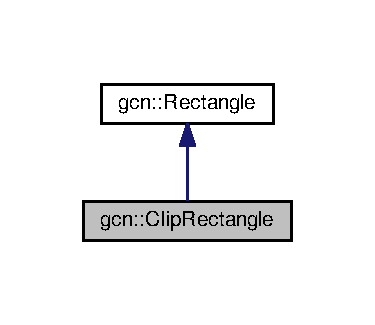
\includegraphics[width=180pt]{classgcn_1_1ClipRectangle__inherit__graph}
\end{center}
\end{figure}


Collaboration diagram for gcn\+:\+:Clip\+Rectangle\+:\nopagebreak
\begin{figure}[H]
\begin{center}
\leavevmode
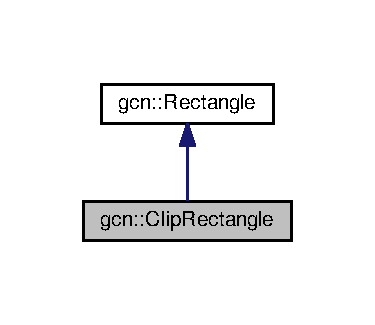
\includegraphics[width=180pt]{classgcn_1_1ClipRectangle__coll__graph}
\end{center}
\end{figure}
\subsection*{Public Member Functions}
\begin{DoxyCompactItemize}
\item 
\hyperlink{classgcn_1_1ClipRectangle_af4b463769706f943b604ceaaf583d27c}{Clip\+Rectangle} ()
\item 
\hyperlink{classgcn_1_1ClipRectangle_a64655edef4076373470ea6146063dd92}{Clip\+Rectangle} (int x, int y, int width, int height, int \hyperlink{classgcn_1_1ClipRectangle_afe946bf9f906a4f571c9a6bdbd9fb730}{x\+Offset}, int \hyperlink{classgcn_1_1ClipRectangle_a322306940b67c677e14cb0cab5b6eb3e}{y\+Offset})
\item 
const \hyperlink{classgcn_1_1ClipRectangle}{Clip\+Rectangle} \& \hyperlink{classgcn_1_1ClipRectangle_af4d051916713471ee1025a5056b47a94}{operator=} (const \hyperlink{classgcn_1_1Rectangle}{Rectangle} \&other)
\end{DoxyCompactItemize}
\subsection*{Public Attributes}
\begin{DoxyCompactItemize}
\item 
int \hyperlink{classgcn_1_1ClipRectangle_afe946bf9f906a4f571c9a6bdbd9fb730}{x\+Offset}
\item 
int \hyperlink{classgcn_1_1ClipRectangle_a322306940b67c677e14cb0cab5b6eb3e}{y\+Offset}
\end{DoxyCompactItemize}


\subsection{Detailed Description}
A rectangle used when dealing with clipping. It is a regular \hyperlink{classgcn_1_1Rectangle}{Rectangle} extended with variables for x offsets and y offsets. 

\subsection{Constructor \& Destructor Documentation}
\index{gcn\+::\+Clip\+Rectangle@{gcn\+::\+Clip\+Rectangle}!Clip\+Rectangle@{Clip\+Rectangle}}
\index{Clip\+Rectangle@{Clip\+Rectangle}!gcn\+::\+Clip\+Rectangle@{gcn\+::\+Clip\+Rectangle}}
\subsubsection[{\texorpdfstring{Clip\+Rectangle()}{ClipRectangle()}}]{\setlength{\rightskip}{0pt plus 5cm}gcn\+::\+Clip\+Rectangle\+::\+Clip\+Rectangle (
\begin{DoxyParamCaption}
{}
\end{DoxyParamCaption}
)}\hypertarget{classgcn_1_1ClipRectangle_af4b463769706f943b604ceaaf583d27c}{}\label{classgcn_1_1ClipRectangle_af4b463769706f943b604ceaaf583d27c}
Constructor. \index{gcn\+::\+Clip\+Rectangle@{gcn\+::\+Clip\+Rectangle}!Clip\+Rectangle@{Clip\+Rectangle}}
\index{Clip\+Rectangle@{Clip\+Rectangle}!gcn\+::\+Clip\+Rectangle@{gcn\+::\+Clip\+Rectangle}}
\subsubsection[{\texorpdfstring{Clip\+Rectangle(int x, int y, int width, int height, int x\+Offset, int y\+Offset)}{ClipRectangle(int x, int y, int width, int height, int xOffset, int yOffset)}}]{\setlength{\rightskip}{0pt plus 5cm}gcn\+::\+Clip\+Rectangle\+::\+Clip\+Rectangle (
\begin{DoxyParamCaption}
\item[{int}]{x, }
\item[{int}]{y, }
\item[{int}]{width, }
\item[{int}]{height, }
\item[{int}]{x\+Offset, }
\item[{int}]{y\+Offset}
\end{DoxyParamCaption}
)}\hypertarget{classgcn_1_1ClipRectangle_a64655edef4076373470ea6146063dd92}{}\label{classgcn_1_1ClipRectangle_a64655edef4076373470ea6146063dd92}
Constructor.


\begin{DoxyParams}{Parameters}
{\em x} & the rectangle x coordinate. \\
\hline
{\em y} & the rectangle y coordinate. \\
\hline
{\em width} & the rectangle width. \\
\hline
{\em height} & the rectangle height. \\
\hline
{\em x\+Offset} & origin of drawing (used by \hyperlink{classgcn_1_1Graphics}{Graphics}). \\
\hline
{\em y\+Offset} & origin of drawing (used by \hyperlink{classgcn_1_1Graphics}{Graphics}) . \\
\hline
\end{DoxyParams}


\subsection{Member Function Documentation}
\index{gcn\+::\+Clip\+Rectangle@{gcn\+::\+Clip\+Rectangle}!operator=@{operator=}}
\index{operator=@{operator=}!gcn\+::\+Clip\+Rectangle@{gcn\+::\+Clip\+Rectangle}}
\subsubsection[{\texorpdfstring{operator=(const Rectangle \&other)}{operator=(const Rectangle &other)}}]{\setlength{\rightskip}{0pt plus 5cm}const {\bf Clip\+Rectangle} \& gcn\+::\+Clip\+Rectangle\+::operator= (
\begin{DoxyParamCaption}
\item[{const {\bf Rectangle} \&}]{other}
\end{DoxyParamCaption}
)}\hypertarget{classgcn_1_1ClipRectangle_af4d051916713471ee1025a5056b47a94}{}\label{classgcn_1_1ClipRectangle_af4d051916713471ee1025a5056b47a94}
Copies x, y, width and height field from a \hyperlink{classgcn_1_1Rectangle}{Rectangle}.


\begin{DoxyParams}{Parameters}
{\em other} & the \hyperlink{classgcn_1_1Rectangle}{Rectangle} to copy from. \\
\hline
\end{DoxyParams}
\begin{DoxyReturn}{Returns}
a \hyperlink{classgcn_1_1ClipRectangle}{Clip\+Rectangle}. 
\end{DoxyReturn}


\subsection{Member Data Documentation}
\index{gcn\+::\+Clip\+Rectangle@{gcn\+::\+Clip\+Rectangle}!x\+Offset@{x\+Offset}}
\index{x\+Offset@{x\+Offset}!gcn\+::\+Clip\+Rectangle@{gcn\+::\+Clip\+Rectangle}}
\subsubsection[{\texorpdfstring{x\+Offset}{xOffset}}]{\setlength{\rightskip}{0pt plus 5cm}int gcn\+::\+Clip\+Rectangle\+::x\+Offset}\hypertarget{classgcn_1_1ClipRectangle_afe946bf9f906a4f571c9a6bdbd9fb730}{}\label{classgcn_1_1ClipRectangle_afe946bf9f906a4f571c9a6bdbd9fb730}
x-\/origin of drawing (used by \hyperlink{classgcn_1_1Graphics}{Graphics}). \index{gcn\+::\+Clip\+Rectangle@{gcn\+::\+Clip\+Rectangle}!y\+Offset@{y\+Offset}}
\index{y\+Offset@{y\+Offset}!gcn\+::\+Clip\+Rectangle@{gcn\+::\+Clip\+Rectangle}}
\subsubsection[{\texorpdfstring{y\+Offset}{yOffset}}]{\setlength{\rightskip}{0pt plus 5cm}int gcn\+::\+Clip\+Rectangle\+::y\+Offset}\hypertarget{classgcn_1_1ClipRectangle_a322306940b67c677e14cb0cab5b6eb3e}{}\label{classgcn_1_1ClipRectangle_a322306940b67c677e14cb0cab5b6eb3e}
y-\/origin of drawing (used by \hyperlink{classgcn_1_1Graphics}{Graphics}). 

The documentation for this class was generated from the following files\+:\begin{DoxyCompactItemize}
\item 
include/guisan/cliprectangle.\+hpp\item 
src/cliprectangle.\+cpp\end{DoxyCompactItemize}

\hypertarget{classgcn_1_1Color}{}\section{gcn\+:\+:Color Class Reference}
\label{classgcn_1_1Color}\index{gcn\+::\+Color@{gcn\+::\+Color}}


{\ttfamily \#include $<$color.\+hpp$>$}

\subsection*{Public Member Functions}
\begin{DoxyCompactItemize}
\item 
\hyperlink{classgcn_1_1Color_a6dc73fa971bdb60c9e00ae4a69d33275}{Color} ()
\item 
\hyperlink{classgcn_1_1Color_a01d8582df017de59b0cf7c6585a4d345}{Color} (int color)
\item 
\hyperlink{classgcn_1_1Color_ac95423f560a25af45f7910c3e9d57837}{Color} (int \hyperlink{classgcn_1_1Color_a03c8b8fd862f837b5295b3ce28c94a33}{r}, int \hyperlink{classgcn_1_1Color_a13947bb1b79574cfb71580896a311a33}{g}, int \hyperlink{classgcn_1_1Color_a92f745d8f763ef16dcda11a03c44437f}{b}, int \hyperlink{classgcn_1_1Color_a46e7ab30d365efc4314368e01ffd6dbf}{a}=255)
\item 
\hyperlink{classgcn_1_1Color}{Color} \hyperlink{classgcn_1_1Color_a4414dab910cdf604db74fb49155136f7}{operator+} (const \hyperlink{classgcn_1_1Color}{Color} \&color) const 
\item 
\hyperlink{classgcn_1_1Color}{Color} \hyperlink{classgcn_1_1Color_a69b37321a4c87e8b3e0389a9abccfeff}{operator-\/} (const \hyperlink{classgcn_1_1Color}{Color} \&color) const 
\item 
\hyperlink{classgcn_1_1Color}{Color} \hyperlink{classgcn_1_1Color_a46103f408dfca5cf60b7f5b30a064139}{operator$\ast$} (float value) const 
\item 
bool \hyperlink{classgcn_1_1Color_aad86f1535915cf79442a9ed14c9f58ed}{operator==} (const \hyperlink{classgcn_1_1Color}{Color} \&color) const 
\item 
bool \hyperlink{classgcn_1_1Color_a0050e2fdab7df61d8c17e19cc2b9c4b3}{operator!=} (const \hyperlink{classgcn_1_1Color}{Color} \&color) const 
\end{DoxyCompactItemize}
\subsection*{Public Attributes}
\begin{DoxyCompactItemize}
\item 
int \hyperlink{classgcn_1_1Color_a03c8b8fd862f837b5295b3ce28c94a33}{r}
\item 
int \hyperlink{classgcn_1_1Color_a13947bb1b79574cfb71580896a311a33}{g}
\item 
int \hyperlink{classgcn_1_1Color_a92f745d8f763ef16dcda11a03c44437f}{b}
\item 
int \hyperlink{classgcn_1_1Color_a46e7ab30d365efc4314368e01ffd6dbf}{a}
\end{DoxyCompactItemize}


\subsection{Detailed Description}
Represents a color with red, green, blue and alpha components. 

\subsection{Constructor \& Destructor Documentation}
\index{gcn\+::\+Color@{gcn\+::\+Color}!Color@{Color}}
\index{Color@{Color}!gcn\+::\+Color@{gcn\+::\+Color}}
\subsubsection[{\texorpdfstring{Color()}{Color()}}]{\setlength{\rightskip}{0pt plus 5cm}gcn\+::\+Color\+::\+Color (
\begin{DoxyParamCaption}
{}
\end{DoxyParamCaption}
)}\hypertarget{classgcn_1_1Color_a6dc73fa971bdb60c9e00ae4a69d33275}{}\label{classgcn_1_1Color_a6dc73fa971bdb60c9e00ae4a69d33275}
Constructor. Initializes the color to black. \index{gcn\+::\+Color@{gcn\+::\+Color}!Color@{Color}}
\index{Color@{Color}!gcn\+::\+Color@{gcn\+::\+Color}}
\subsubsection[{\texorpdfstring{Color(int color)}{Color(int color)}}]{\setlength{\rightskip}{0pt plus 5cm}gcn\+::\+Color\+::\+Color (
\begin{DoxyParamCaption}
\item[{int}]{color}
\end{DoxyParamCaption}
)}\hypertarget{classgcn_1_1Color_a01d8582df017de59b0cf7c6585a4d345}{}\label{classgcn_1_1Color_a01d8582df017de59b0cf7c6585a4d345}
Constructs a color from the bytes in an integer. Call it with a hexadecimal constant for H\+T\+M\+L-\/style color representation. The alpha component will be set to 255.

E\+X\+A\+M\+P\+LE\+: Color(0xff50a0) constructs Gui-\/chan\textquotesingle{}s favourite color.

N\+O\+TE\+: Because of this constructor, integers will be automatically casted to a color by your compiler.


\begin{DoxyParams}{Parameters}
{\em color} & the color. \\
\hline
\end{DoxyParams}
\index{gcn\+::\+Color@{gcn\+::\+Color}!Color@{Color}}
\index{Color@{Color}!gcn\+::\+Color@{gcn\+::\+Color}}
\subsubsection[{\texorpdfstring{Color(int r, int g, int b, int a=255)}{Color(int r, int g, int b, int a=255)}}]{\setlength{\rightskip}{0pt plus 5cm}gcn\+::\+Color\+::\+Color (
\begin{DoxyParamCaption}
\item[{int}]{r, }
\item[{int}]{g, }
\item[{int}]{b, }
\item[{int}]{a = {\ttfamily 255}}
\end{DoxyParamCaption}
)}\hypertarget{classgcn_1_1Color_ac95423f560a25af45f7910c3e9d57837}{}\label{classgcn_1_1Color_ac95423f560a25af45f7910c3e9d57837}
Constructor.


\begin{DoxyParams}{Parameters}
{\em r} & Red color component (range 0-\/255). \\
\hline
{\em g} & Green color component (range 0-\/255). \\
\hline
{\em b} & Blue color component (range 0-\/255). \\
\hline
{\em a} & \hyperlink{classgcn_1_1Color}{Color} alpha, used for transparency. A value of 0 means totaly transparent, 255 is totaly opaque (the default). \\
\hline
\end{DoxyParams}


\subsection{Member Function Documentation}
\index{gcn\+::\+Color@{gcn\+::\+Color}!operator"!=@{operator"!=}}
\index{operator"!=@{operator"!=}!gcn\+::\+Color@{gcn\+::\+Color}}
\subsubsection[{\texorpdfstring{operator"!=(const Color \&color) const }{operator!=(const Color &color) const }}]{\setlength{\rightskip}{0pt plus 5cm}bool gcn\+::\+Color\+::operator!= (
\begin{DoxyParamCaption}
\item[{const {\bf Color} \&}]{color}
\end{DoxyParamCaption}
) const}\hypertarget{classgcn_1_1Color_a0050e2fdab7df61d8c17e19cc2b9c4b3}{}\label{classgcn_1_1Color_a0050e2fdab7df61d8c17e19cc2b9c4b3}
Compares two colors.

\begin{DoxyReturn}{Returns}
true if the two colors have different R\+G\+BA components. 
\end{DoxyReturn}
\index{gcn\+::\+Color@{gcn\+::\+Color}!operator$\ast$@{operator$\ast$}}
\index{operator$\ast$@{operator$\ast$}!gcn\+::\+Color@{gcn\+::\+Color}}
\subsubsection[{\texorpdfstring{operator$\ast$(float value) const }{operator*(float value) const }}]{\setlength{\rightskip}{0pt plus 5cm}{\bf Color} gcn\+::\+Color\+::operator$\ast$ (
\begin{DoxyParamCaption}
\item[{float}]{value}
\end{DoxyParamCaption}
) const}\hypertarget{classgcn_1_1Color_a46103f408dfca5cf60b7f5b30a064139}{}\label{classgcn_1_1Color_a46103f408dfca5cf60b7f5b30a064139}
Multiplies the R\+GB values of a color with a float value. The values will be clamped if they go out of range.


\begin{DoxyParams}{Parameters}
{\em value} & the value to multiply the color with. \\
\hline
\end{DoxyParams}
\begin{DoxyReturn}{Returns}
the resulting color with alpha untouched. 
\end{DoxyReturn}
\index{gcn\+::\+Color@{gcn\+::\+Color}!operator+@{operator+}}
\index{operator+@{operator+}!gcn\+::\+Color@{gcn\+::\+Color}}
\subsubsection[{\texorpdfstring{operator+(const Color \&color) const }{operator+(const Color &color) const }}]{\setlength{\rightskip}{0pt plus 5cm}{\bf Color} gcn\+::\+Color\+::operator+ (
\begin{DoxyParamCaption}
\item[{const {\bf Color} \&}]{color}
\end{DoxyParamCaption}
) const}\hypertarget{classgcn_1_1Color_a4414dab910cdf604db74fb49155136f7}{}\label{classgcn_1_1Color_a4414dab910cdf604db74fb49155136f7}
Adds the R\+GB values of two colors together. The values will be clamped if they go out of range.


\begin{DoxyParams}{Parameters}
{\em color} & a color to add to this color. \\
\hline
\end{DoxyParams}
\begin{DoxyReturn}{Returns}
the resulting color with alpha set to 255. 
\end{DoxyReturn}
\index{gcn\+::\+Color@{gcn\+::\+Color}!operator-\/@{operator-\/}}
\index{operator-\/@{operator-\/}!gcn\+::\+Color@{gcn\+::\+Color}}
\subsubsection[{\texorpdfstring{operator-\/(const Color \&color) const }{operator-(const Color &color) const }}]{\setlength{\rightskip}{0pt plus 5cm}{\bf Color} gcn\+::\+Color\+::operator-\/ (
\begin{DoxyParamCaption}
\item[{const {\bf Color} \&}]{color}
\end{DoxyParamCaption}
) const}\hypertarget{classgcn_1_1Color_a69b37321a4c87e8b3e0389a9abccfeff}{}\label{classgcn_1_1Color_a69b37321a4c87e8b3e0389a9abccfeff}
Subtracts the R\+GB values of one color from another. The values will be clamped if they go out of range.


\begin{DoxyParams}{Parameters}
{\em color} & a color to subtract from this color. \\
\hline
\end{DoxyParams}
\begin{DoxyReturn}{Returns}
the resulting color with alpha set to 255. 
\end{DoxyReturn}
\index{gcn\+::\+Color@{gcn\+::\+Color}!operator==@{operator==}}
\index{operator==@{operator==}!gcn\+::\+Color@{gcn\+::\+Color}}
\subsubsection[{\texorpdfstring{operator==(const Color \&color) const }{operator==(const Color &color) const }}]{\setlength{\rightskip}{0pt plus 5cm}bool gcn\+::\+Color\+::operator== (
\begin{DoxyParamCaption}
\item[{const {\bf Color} \&}]{color}
\end{DoxyParamCaption}
) const}\hypertarget{classgcn_1_1Color_aad86f1535915cf79442a9ed14c9f58ed}{}\label{classgcn_1_1Color_aad86f1535915cf79442a9ed14c9f58ed}
Compares two colors.

\begin{DoxyReturn}{Returns}
true if the two colors have the same R\+G\+BA components. 
\end{DoxyReturn}


\subsection{Member Data Documentation}
\index{gcn\+::\+Color@{gcn\+::\+Color}!a@{a}}
\index{a@{a}!gcn\+::\+Color@{gcn\+::\+Color}}
\subsubsection[{\texorpdfstring{a}{a}}]{\setlength{\rightskip}{0pt plus 5cm}int gcn\+::\+Color\+::a}\hypertarget{classgcn_1_1Color_a46e7ab30d365efc4314368e01ffd6dbf}{}\label{classgcn_1_1Color_a46e7ab30d365efc4314368e01ffd6dbf}
\hyperlink{classgcn_1_1Color}{Color} alpha, used for transparency. A value of 0 means totaly transparent, 255 is totaly opaque (the default) \index{gcn\+::\+Color@{gcn\+::\+Color}!b@{b}}
\index{b@{b}!gcn\+::\+Color@{gcn\+::\+Color}}
\subsubsection[{\texorpdfstring{b}{b}}]{\setlength{\rightskip}{0pt plus 5cm}int gcn\+::\+Color\+::b}\hypertarget{classgcn_1_1Color_a92f745d8f763ef16dcda11a03c44437f}{}\label{classgcn_1_1Color_a92f745d8f763ef16dcda11a03c44437f}
Blue color component (range 0-\/255). \index{gcn\+::\+Color@{gcn\+::\+Color}!g@{g}}
\index{g@{g}!gcn\+::\+Color@{gcn\+::\+Color}}
\subsubsection[{\texorpdfstring{g}{g}}]{\setlength{\rightskip}{0pt plus 5cm}int gcn\+::\+Color\+::g}\hypertarget{classgcn_1_1Color_a13947bb1b79574cfb71580896a311a33}{}\label{classgcn_1_1Color_a13947bb1b79574cfb71580896a311a33}
Green color component (range 0-\/255). \index{gcn\+::\+Color@{gcn\+::\+Color}!r@{r}}
\index{r@{r}!gcn\+::\+Color@{gcn\+::\+Color}}
\subsubsection[{\texorpdfstring{r}{r}}]{\setlength{\rightskip}{0pt plus 5cm}int gcn\+::\+Color\+::r}\hypertarget{classgcn_1_1Color_a03c8b8fd862f837b5295b3ce28c94a33}{}\label{classgcn_1_1Color_a03c8b8fd862f837b5295b3ce28c94a33}
Red color component (range 0-\/255). 

The documentation for this class was generated from the following files\+:\begin{DoxyCompactItemize}
\item 
include/guisan/color.\+hpp\item 
src/color.\+cpp\end{DoxyCompactItemize}

\hypertarget{classgcn_1_1Container}{}\section{gcn\+:\+:Container Class Reference}
\label{classgcn_1_1Container}\index{gcn\+::\+Container@{gcn\+::\+Container}}


{\ttfamily \#include $<$container.\+hpp$>$}



Inheritance diagram for gcn\+:\+:Container\+:\nopagebreak
\begin{figure}[H]
\begin{center}
\leavevmode
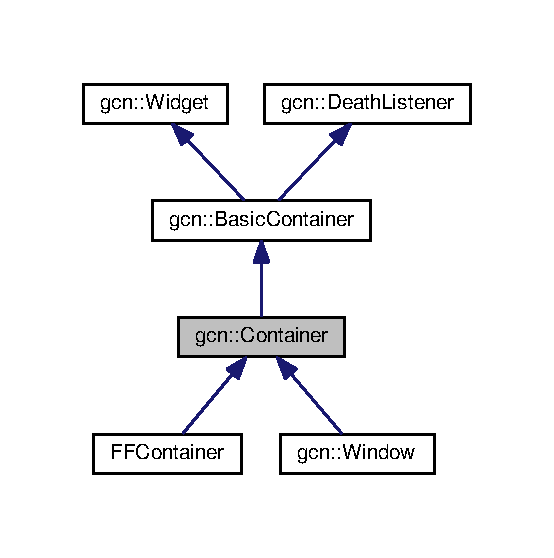
\includegraphics[width=266pt]{classgcn_1_1Container__inherit__graph}
\end{center}
\end{figure}


Collaboration diagram for gcn\+:\+:Container\+:\nopagebreak
\begin{figure}[H]
\begin{center}
\leavevmode
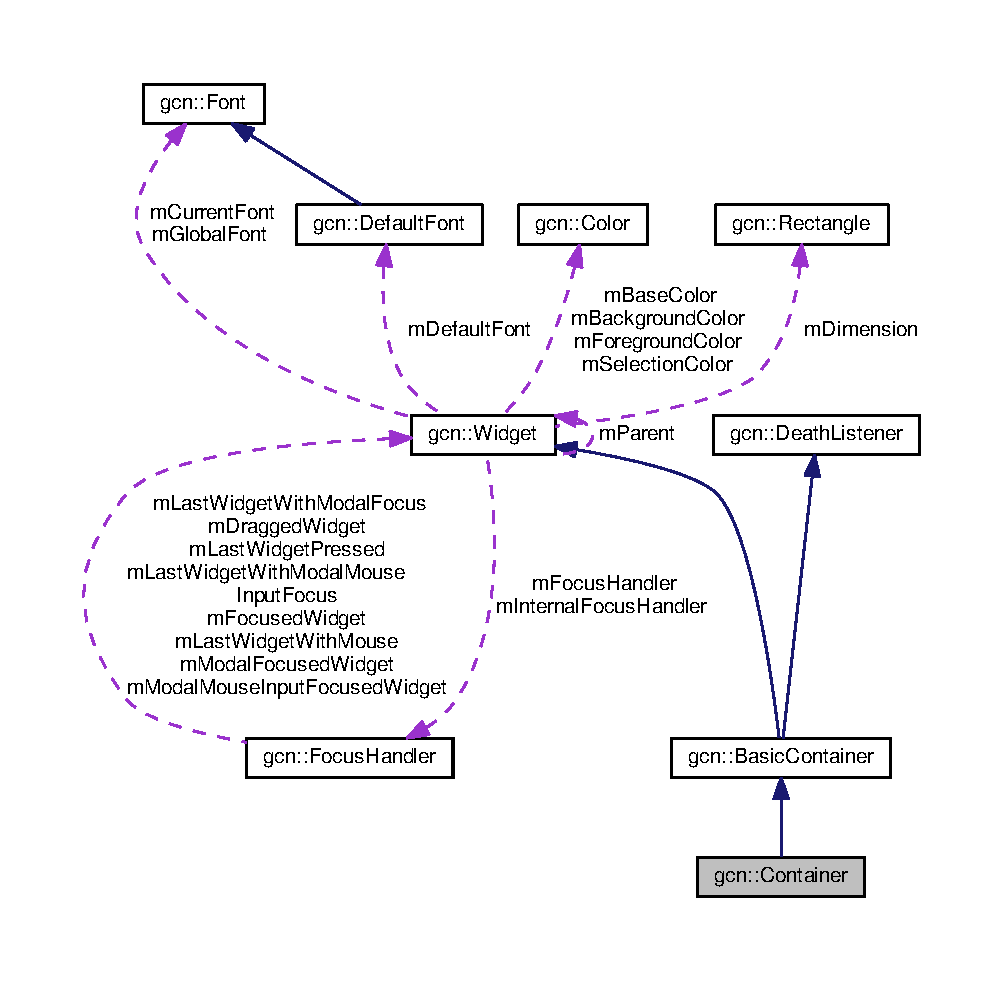
\includegraphics[width=350pt]{classgcn_1_1Container__coll__graph}
\end{center}
\end{figure}
\subsection*{Public Member Functions}
\begin{DoxyCompactItemize}
\item 
\hyperlink{classgcn_1_1Container_a9b7bc2cf017eb3ed6a855688cf57322a}{Container} ()
\item 
virtual \hyperlink{classgcn_1_1Container_a3384a372ea00af8cce5b88dd614a9b30}{$\sim$\+Container} ()
\item 
void \hyperlink{classgcn_1_1Container_ae98ebff48adcfc7f95ac44b28864f36a}{set\+Opaque} (bool opaque)
\item 
bool \hyperlink{classgcn_1_1Container_a458c9f8e2a6dd5373e666a6fe62ec719}{is\+Opaque} () const 
\item 
virtual void \hyperlink{classgcn_1_1Container_a183a60d39fc503b7e37c71491105f766}{add} (\hyperlink{classgcn_1_1Widget}{Widget} $\ast$widget)
\item 
virtual void \hyperlink{classgcn_1_1Container_aa78a475e596e8261d4187ef58338e5ab}{add} (\hyperlink{classgcn_1_1Widget}{Widget} $\ast$widget, int x, int y)
\item 
virtual void \hyperlink{classgcn_1_1Container_a6ed5e946da5112c8b86d708c9000274e}{remove} (\hyperlink{classgcn_1_1Widget}{Widget} $\ast$widget)
\item 
virtual void \hyperlink{classgcn_1_1Container_a561436ebcebc3419545a4db3397c6686}{clear} ()
\item 
virtual \hyperlink{classgcn_1_1Widget}{Widget} $\ast$ \hyperlink{classgcn_1_1Container_a7871002a444dba6ad82df1dcef61561b}{find\+Widget\+By\+Id} (const std\+::string \&id)
\item 
virtual void \hyperlink{classgcn_1_1Container_a0bc3386f5564165fcb13e9d389a96432}{draw} (\hyperlink{classgcn_1_1Graphics}{Graphics} $\ast$graphics)
\item 
virtual void \hyperlink{classgcn_1_1Container_a0bb6aecc841e06a887f32905b561180b}{draw\+Border} (\hyperlink{classgcn_1_1Graphics}{Graphics} $\ast$graphics)
\end{DoxyCompactItemize}
\subsection*{Protected Attributes}
\begin{DoxyCompactItemize}
\item 
bool \hyperlink{classgcn_1_1Container_a4fd62e01a8196c69c83e751af45a5ade}{m\+Opaque}
\end{DoxyCompactItemize}
\subsection*{Additional Inherited Members}


\subsection{Detailed Description}
An implementation of a container able to contain other widgets. A widget\textquotesingle{}s position in the container is relative to the container itself and not the screen. A container is the most common widget to use as the \hyperlink{classgcn_1_1Gui}{Gui}\textquotesingle{}s top widget as makes the \hyperlink{classgcn_1_1Gui}{Gui} able to contain more than one widget.

\begin{DoxySeeAlso}{See also}
\hyperlink{classgcn_1_1Gui_a69ce39ec8962ae93f428a01ffec677de}{Gui\+::set\+Top} 
\end{DoxySeeAlso}


\subsection{Constructor \& Destructor Documentation}
\index{gcn\+::\+Container@{gcn\+::\+Container}!Container@{Container}}
\index{Container@{Container}!gcn\+::\+Container@{gcn\+::\+Container}}
\subsubsection[{\texorpdfstring{Container()}{Container()}}]{\setlength{\rightskip}{0pt plus 5cm}gcn\+::\+Container\+::\+Container (
\begin{DoxyParamCaption}
{}
\end{DoxyParamCaption}
)}\hypertarget{classgcn_1_1Container_a9b7bc2cf017eb3ed6a855688cf57322a}{}\label{classgcn_1_1Container_a9b7bc2cf017eb3ed6a855688cf57322a}
Constructor. A container is opauqe as default, if you want a none opaque container call set\+Qpaque(false).

\begin{DoxySeeAlso}{See also}
\hyperlink{classgcn_1_1Container_ae98ebff48adcfc7f95ac44b28864f36a}{set\+Opaque}, \hyperlink{classgcn_1_1Container_a458c9f8e2a6dd5373e666a6fe62ec719}{is\+Opaque} 
\end{DoxySeeAlso}
\index{gcn\+::\+Container@{gcn\+::\+Container}!````~Container@{$\sim$\+Container}}
\index{````~Container@{$\sim$\+Container}!gcn\+::\+Container@{gcn\+::\+Container}}
\subsubsection[{\texorpdfstring{$\sim$\+Container()}{~Container()}}]{\setlength{\rightskip}{0pt plus 5cm}gcn\+::\+Container\+::$\sim$\+Container (
\begin{DoxyParamCaption}
{}
\end{DoxyParamCaption}
)\hspace{0.3cm}{\ttfamily [virtual]}}\hypertarget{classgcn_1_1Container_a3384a372ea00af8cce5b88dd614a9b30}{}\label{classgcn_1_1Container_a3384a372ea00af8cce5b88dd614a9b30}
Destructor. 

\subsection{Member Function Documentation}
\index{gcn\+::\+Container@{gcn\+::\+Container}!add@{add}}
\index{add@{add}!gcn\+::\+Container@{gcn\+::\+Container}}
\subsubsection[{\texorpdfstring{add(\+Widget $\ast$widget)}{add(Widget *widget)}}]{\setlength{\rightskip}{0pt plus 5cm}void gcn\+::\+Container\+::add (
\begin{DoxyParamCaption}
\item[{{\bf Widget} $\ast$}]{widget}
\end{DoxyParamCaption}
)\hspace{0.3cm}{\ttfamily [virtual]}}\hypertarget{classgcn_1_1Container_a183a60d39fc503b7e37c71491105f766}{}\label{classgcn_1_1Container_a183a60d39fc503b7e37c71491105f766}
Adds a widget to the container.


\begin{DoxyParams}{Parameters}
{\em widget} & The widget to add. \\
\hline
\end{DoxyParams}
\begin{DoxySeeAlso}{See also}
\hyperlink{classgcn_1_1Container_a6ed5e946da5112c8b86d708c9000274e}{remove}, \hyperlink{classgcn_1_1Container_a561436ebcebc3419545a4db3397c6686}{clear} 
\end{DoxySeeAlso}
\index{gcn\+::\+Container@{gcn\+::\+Container}!add@{add}}
\index{add@{add}!gcn\+::\+Container@{gcn\+::\+Container}}
\subsubsection[{\texorpdfstring{add(\+Widget $\ast$widget, int x, int y)}{add(Widget *widget, int x, int y)}}]{\setlength{\rightskip}{0pt plus 5cm}void gcn\+::\+Container\+::add (
\begin{DoxyParamCaption}
\item[{{\bf Widget} $\ast$}]{widget, }
\item[{int}]{x, }
\item[{int}]{y}
\end{DoxyParamCaption}
)\hspace{0.3cm}{\ttfamily [virtual]}}\hypertarget{classgcn_1_1Container_aa78a475e596e8261d4187ef58338e5ab}{}\label{classgcn_1_1Container_aa78a475e596e8261d4187ef58338e5ab}
Adds a widget to the container and also specifices the widget\textquotesingle{}s postion in the container. The position is relative to the container and not relative to the screen.


\begin{DoxyParams}{Parameters}
{\em widget} & The widget to add. \\
\hline
{\em x} & The x coordinat for the widget. \\
\hline
{\em y} & The y coordinat for the widget. \\
\hline
\end{DoxyParams}
\begin{DoxySeeAlso}{See also}
\hyperlink{classgcn_1_1Container_a6ed5e946da5112c8b86d708c9000274e}{remove}, \hyperlink{classgcn_1_1Container_a561436ebcebc3419545a4db3397c6686}{clear} 
\end{DoxySeeAlso}
\index{gcn\+::\+Container@{gcn\+::\+Container}!clear@{clear}}
\index{clear@{clear}!gcn\+::\+Container@{gcn\+::\+Container}}
\subsubsection[{\texorpdfstring{clear()}{clear()}}]{\setlength{\rightskip}{0pt plus 5cm}void gcn\+::\+Container\+::clear (
\begin{DoxyParamCaption}
{}
\end{DoxyParamCaption}
)\hspace{0.3cm}{\ttfamily [virtual]}}\hypertarget{classgcn_1_1Container_a561436ebcebc3419545a4db3397c6686}{}\label{classgcn_1_1Container_a561436ebcebc3419545a4db3397c6686}
Clears the container of all widgets.

\begin{DoxySeeAlso}{See also}
\hyperlink{classgcn_1_1Container_a183a60d39fc503b7e37c71491105f766}{add}, \hyperlink{classgcn_1_1Container_a6ed5e946da5112c8b86d708c9000274e}{remove} 
\end{DoxySeeAlso}


Reimplemented from \hyperlink{classgcn_1_1BasicContainer_a6b494b3e7c7369efcfc0e3f2f964bcf8}{gcn\+::\+Basic\+Container}.

\index{gcn\+::\+Container@{gcn\+::\+Container}!draw@{draw}}
\index{draw@{draw}!gcn\+::\+Container@{gcn\+::\+Container}}
\subsubsection[{\texorpdfstring{draw(\+Graphics $\ast$graphics)}{draw(Graphics *graphics)}}]{\setlength{\rightskip}{0pt plus 5cm}void gcn\+::\+Container\+::draw (
\begin{DoxyParamCaption}
\item[{{\bf Graphics} $\ast$}]{graphics}
\end{DoxyParamCaption}
)\hspace{0.3cm}{\ttfamily [virtual]}}\hypertarget{classgcn_1_1Container_a0bc3386f5564165fcb13e9d389a96432}{}\label{classgcn_1_1Container_a0bc3386f5564165fcb13e9d389a96432}
Draws the widget. It is called by the parent widget when it is time for the widget to draw itself. The graphics object is set up so that all drawing is relative to the widget, i.\+e coordinate (0,0) is the top-\/left corner of the widget. It is not possible to draw outside of a widgets dimension.


\begin{DoxyParams}{Parameters}
{\em graphics} & a \hyperlink{classgcn_1_1Graphics}{Graphics} object to draw with. \\
\hline
\end{DoxyParams}


Implements \hyperlink{classgcn_1_1Widget_acc595221d6a2d1afe1043c16dc37d212}{gcn\+::\+Widget}.



Reimplemented in \hyperlink{classgcn_1_1Window_a6d41ec33f8d4389510a9071067c919e5}{gcn\+::\+Window}, and \hyperlink{classFFContainer_a42352820e4ed070f831a84a8b51451c6}{F\+F\+Container}.

\index{gcn\+::\+Container@{gcn\+::\+Container}!draw\+Border@{draw\+Border}}
\index{draw\+Border@{draw\+Border}!gcn\+::\+Container@{gcn\+::\+Container}}
\subsubsection[{\texorpdfstring{draw\+Border(\+Graphics $\ast$graphics)}{drawBorder(Graphics *graphics)}}]{\setlength{\rightskip}{0pt plus 5cm}void gcn\+::\+Container\+::draw\+Border (
\begin{DoxyParamCaption}
\item[{{\bf Graphics} $\ast$}]{graphics}
\end{DoxyParamCaption}
)\hspace{0.3cm}{\ttfamily [virtual]}}\hypertarget{classgcn_1_1Container_a0bb6aecc841e06a887f32905b561180b}{}\label{classgcn_1_1Container_a0bb6aecc841e06a887f32905b561180b}
Draws the widget border. A border is drawn around a widget. The width and height of the border is therefore the widgets height+2$\ast$bordersize. Think of a painting that has a certain size, the border surrounds the painting.


\begin{DoxyParams}{Parameters}
{\em graphics} & a \hyperlink{classgcn_1_1Graphics}{Graphics} object to draw with. \\
\hline
\end{DoxyParams}


Reimplemented from \hyperlink{classgcn_1_1Widget_a58c3b2f513d8e029e321fd88a974f5c4}{gcn\+::\+Widget}.



Reimplemented in \hyperlink{classgcn_1_1Window_ae5564549656568a7932811e0f4025113}{gcn\+::\+Window}.

\index{gcn\+::\+Container@{gcn\+::\+Container}!find\+Widget\+By\+Id@{find\+Widget\+By\+Id}}
\index{find\+Widget\+By\+Id@{find\+Widget\+By\+Id}!gcn\+::\+Container@{gcn\+::\+Container}}
\subsubsection[{\texorpdfstring{find\+Widget\+By\+Id(const std\+::string \&id)}{findWidgetById(const std::string &id)}}]{\setlength{\rightskip}{0pt plus 5cm}{\bf Widget} $\ast$ gcn\+::\+Container\+::find\+Widget\+By\+Id (
\begin{DoxyParamCaption}
\item[{const std\+::string \&}]{id}
\end{DoxyParamCaption}
)\hspace{0.3cm}{\ttfamily [virtual]}}\hypertarget{classgcn_1_1Container_a7871002a444dba6ad82df1dcef61561b}{}\label{classgcn_1_1Container_a7871002a444dba6ad82df1dcef61561b}
Finds a widget given an id.


\begin{DoxyParams}{Parameters}
{\em id} & The id to find a widget by. \\
\hline
\end{DoxyParams}
\begin{DoxyReturn}{Returns}
A widget with a corrosponding id, N\+U\+LL if no widget is found. 
\end{DoxyReturn}
\begin{DoxySeeAlso}{See also}
\hyperlink{classgcn_1_1Widget_a0f3484b135d2c21f1d779e37f7ee4cd3}{Widget\+::set\+Id} 
\end{DoxySeeAlso}


Reimplemented from \hyperlink{classgcn_1_1BasicContainer_a4c734912bb5342259dc7bd77d606bd7e}{gcn\+::\+Basic\+Container}.

\index{gcn\+::\+Container@{gcn\+::\+Container}!is\+Opaque@{is\+Opaque}}
\index{is\+Opaque@{is\+Opaque}!gcn\+::\+Container@{gcn\+::\+Container}}
\subsubsection[{\texorpdfstring{is\+Opaque() const }{isOpaque() const }}]{\setlength{\rightskip}{0pt plus 5cm}bool gcn\+::\+Container\+::is\+Opaque (
\begin{DoxyParamCaption}
{}
\end{DoxyParamCaption}
) const}\hypertarget{classgcn_1_1Container_a458c9f8e2a6dd5373e666a6fe62ec719}{}\label{classgcn_1_1Container_a458c9f8e2a6dd5373e666a6fe62ec719}
Checks if the container is opaque or not.

\begin{DoxyReturn}{Returns}
true if the container is opaque, false otherwise. 
\end{DoxyReturn}
\begin{DoxySeeAlso}{See also}
\hyperlink{classgcn_1_1Container_ae98ebff48adcfc7f95ac44b28864f36a}{set\+Opaque} 
\end{DoxySeeAlso}
\index{gcn\+::\+Container@{gcn\+::\+Container}!remove@{remove}}
\index{remove@{remove}!gcn\+::\+Container@{gcn\+::\+Container}}
\subsubsection[{\texorpdfstring{remove(\+Widget $\ast$widget)}{remove(Widget *widget)}}]{\setlength{\rightskip}{0pt plus 5cm}void gcn\+::\+Container\+::remove (
\begin{DoxyParamCaption}
\item[{{\bf Widget} $\ast$}]{widget}
\end{DoxyParamCaption}
)\hspace{0.3cm}{\ttfamily [virtual]}}\hypertarget{classgcn_1_1Container_a6ed5e946da5112c8b86d708c9000274e}{}\label{classgcn_1_1Container_a6ed5e946da5112c8b86d708c9000274e}
Removes a widget from the \hyperlink{classgcn_1_1Container}{Container}.


\begin{DoxyParams}{Parameters}
{\em widget} & The widget to remove. \\
\hline
\end{DoxyParams}

\begin{DoxyExceptions}{Exceptions}
{\em \hyperlink{classgcn_1_1Exception}{Exception}} & when the widget has not been added to the container. \\
\hline
\end{DoxyExceptions}
\begin{DoxySeeAlso}{See also}
\hyperlink{classgcn_1_1Container_a183a60d39fc503b7e37c71491105f766}{add}, \hyperlink{classgcn_1_1Container_a561436ebcebc3419545a4db3397c6686}{clear} 
\end{DoxySeeAlso}


Reimplemented from \hyperlink{classgcn_1_1BasicContainer_a1e834058961f0cf6d1eea415ca509b10}{gcn\+::\+Basic\+Container}.

\index{gcn\+::\+Container@{gcn\+::\+Container}!set\+Opaque@{set\+Opaque}}
\index{set\+Opaque@{set\+Opaque}!gcn\+::\+Container@{gcn\+::\+Container}}
\subsubsection[{\texorpdfstring{set\+Opaque(bool opaque)}{setOpaque(bool opaque)}}]{\setlength{\rightskip}{0pt plus 5cm}void gcn\+::\+Container\+::set\+Opaque (
\begin{DoxyParamCaption}
\item[{bool}]{opaque}
\end{DoxyParamCaption}
)}\hypertarget{classgcn_1_1Container_ae98ebff48adcfc7f95ac44b28864f36a}{}\label{classgcn_1_1Container_ae98ebff48adcfc7f95ac44b28864f36a}
Sets the container to be opaque or not. If the container is opaque it\textquotesingle{}s background will be drawn, if it\textquotesingle{}s not opaque it\textquotesingle{}s background will not be drawn, and thus making the container completely transparent.

N\+O\+TE\+: This is not the same as to set visibility. A non visible container will not itself nor will it draw it\textquotesingle{}s content.


\begin{DoxyParams}{Parameters}
{\em opaque} & True if the container should be opaque, false otherwise. \\
\hline
\end{DoxyParams}
\begin{DoxySeeAlso}{See also}
\hyperlink{classgcn_1_1Container_a458c9f8e2a6dd5373e666a6fe62ec719}{is\+Opaque} 
\end{DoxySeeAlso}


\subsection{Member Data Documentation}
\index{gcn\+::\+Container@{gcn\+::\+Container}!m\+Opaque@{m\+Opaque}}
\index{m\+Opaque@{m\+Opaque}!gcn\+::\+Container@{gcn\+::\+Container}}
\subsubsection[{\texorpdfstring{m\+Opaque}{mOpaque}}]{\setlength{\rightskip}{0pt plus 5cm}bool gcn\+::\+Container\+::m\+Opaque\hspace{0.3cm}{\ttfamily [protected]}}\hypertarget{classgcn_1_1Container_a4fd62e01a8196c69c83e751af45a5ade}{}\label{classgcn_1_1Container_a4fd62e01a8196c69c83e751af45a5ade}
True if the container is opaque, false otherwise. 

The documentation for this class was generated from the following files\+:\begin{DoxyCompactItemize}
\item 
include/guisan/widgets/container.\+hpp\item 
src/widgets/container.\+cpp\end{DoxyCompactItemize}

\hypertarget{classgcn_1_1DeathListener}{}\section{gcn\+:\+:Death\+Listener Class Reference}
\label{classgcn_1_1DeathListener}\index{gcn\+::\+Death\+Listener@{gcn\+::\+Death\+Listener}}


{\ttfamily \#include $<$deathlistener.\+hpp$>$}



Inheritance diagram for gcn\+:\+:Death\+Listener\+:\nopagebreak
\begin{figure}[H]
\begin{center}
\leavevmode
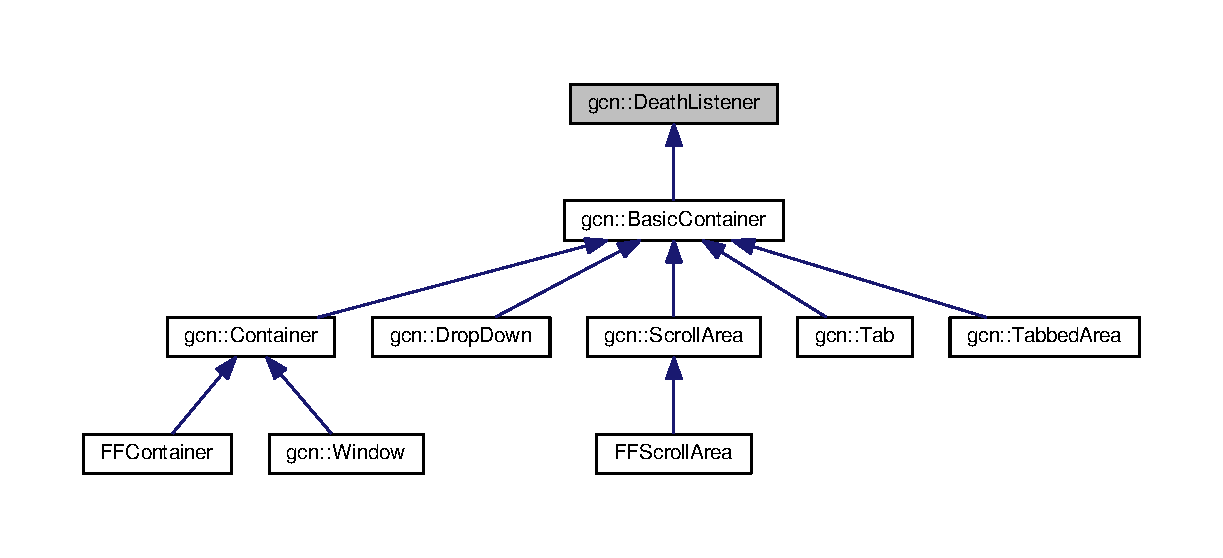
\includegraphics[width=350pt]{classgcn_1_1DeathListener__inherit__graph}
\end{center}
\end{figure}
\subsection*{Public Member Functions}
\begin{DoxyCompactItemize}
\item 
virtual \hyperlink{classgcn_1_1DeathListener_a1372819e4a4a727d00ac32163fb620c4}{$\sim$\+Death\+Listener} ()
\item 
virtual void \hyperlink{classgcn_1_1DeathListener_a526e786e21fcf1266a56f20617babf90}{death} (const \hyperlink{classgcn_1_1Event}{Event} \&event)=0
\end{DoxyCompactItemize}


\subsection{Detailed Description}
Listener of death events from Widgets. To be able to listen for deaths you must make a class which inherits from this class and implements the death function.

\begin{DoxySeeAlso}{See also}
\hyperlink{classgcn_1_1Widget_a874a4f734daddf0fdc4d9d70ebb1ee26}{Widget\+::add\+Death\+Listener} 
\end{DoxySeeAlso}
\begin{DoxyAuthor}{Author}
Olof Naess�n 
\end{DoxyAuthor}
\begin{DoxySince}{Since}
0.\+6.\+0 
\end{DoxySince}


\subsection{Constructor \& Destructor Documentation}
\index{gcn\+::\+Death\+Listener@{gcn\+::\+Death\+Listener}!````~Death\+Listener@{$\sim$\+Death\+Listener}}
\index{````~Death\+Listener@{$\sim$\+Death\+Listener}!gcn\+::\+Death\+Listener@{gcn\+::\+Death\+Listener}}
\subsubsection[{\texorpdfstring{$\sim$\+Death\+Listener()}{~DeathListener()}}]{\setlength{\rightskip}{0pt plus 5cm}virtual gcn\+::\+Death\+Listener\+::$\sim$\+Death\+Listener (
\begin{DoxyParamCaption}
{}
\end{DoxyParamCaption}
)\hspace{0.3cm}{\ttfamily [inline]}, {\ttfamily [virtual]}}\hypertarget{classgcn_1_1DeathListener_a1372819e4a4a727d00ac32163fb620c4}{}\label{classgcn_1_1DeathListener_a1372819e4a4a727d00ac32163fb620c4}
Destructor. 

\subsection{Member Function Documentation}
\index{gcn\+::\+Death\+Listener@{gcn\+::\+Death\+Listener}!death@{death}}
\index{death@{death}!gcn\+::\+Death\+Listener@{gcn\+::\+Death\+Listener}}
\subsubsection[{\texorpdfstring{death(const Event \&event)=0}{death(const Event &event)=0}}]{\setlength{\rightskip}{0pt plus 5cm}virtual void gcn\+::\+Death\+Listener\+::death (
\begin{DoxyParamCaption}
\item[{const {\bf Event} \&}]{event}
\end{DoxyParamCaption}
)\hspace{0.3cm}{\ttfamily [pure virtual]}}\hypertarget{classgcn_1_1DeathListener_a526e786e21fcf1266a56f20617babf90}{}\label{classgcn_1_1DeathListener_a526e786e21fcf1266a56f20617babf90}
Called when a widget dies. It is used to be able to recieve a notification when a death of a widget occurs.


\begin{DoxyParams}{Parameters}
{\em event} & the event of the death. \\
\hline
\end{DoxyParams}


Implemented in \hyperlink{classgcn_1_1DropDown_a8f6402e1ad3ac77b7db296bbd77a7494}{gcn\+::\+Drop\+Down}, \hyperlink{classgcn_1_1TabbedArea_aacf206f5ea02e67b295b7b26ea2a6eac}{gcn\+::\+Tabbed\+Area}, and \hyperlink{classgcn_1_1BasicContainer_ac6cf8760537dcd167e0f518f556bccf4}{gcn\+::\+Basic\+Container}.



The documentation for this class was generated from the following file\+:\begin{DoxyCompactItemize}
\item 
include/guisan/deathlistener.\+hpp\end{DoxyCompactItemize}

\hypertarget{classgcn_1_1DefaultFont}{}\section{gcn\+:\+:Default\+Font Class Reference}
\label{classgcn_1_1DefaultFont}\index{gcn\+::\+Default\+Font@{gcn\+::\+Default\+Font}}


{\ttfamily \#include $<$defaultfont.\+hpp$>$}



Inheritance diagram for gcn\+:\+:Default\+Font\+:\nopagebreak
\begin{figure}[H]
\begin{center}
\leavevmode
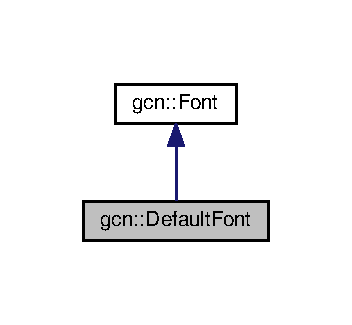
\includegraphics[width=169pt]{classgcn_1_1DefaultFont__inherit__graph}
\end{center}
\end{figure}


Collaboration diagram for gcn\+:\+:Default\+Font\+:\nopagebreak
\begin{figure}[H]
\begin{center}
\leavevmode
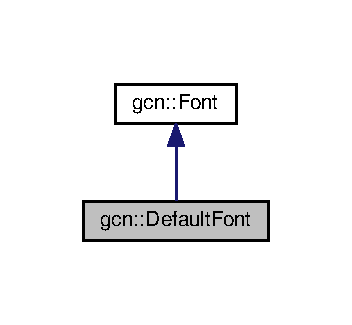
\includegraphics[width=169pt]{classgcn_1_1DefaultFont__coll__graph}
\end{center}
\end{figure}
\subsection*{Public Member Functions}
\begin{DoxyCompactItemize}
\item 
virtual \hyperlink{classgcn_1_1DefaultFont_ab606ee0708758b5fafd19cfc8938b624}{$\sim$\+Default\+Font} ()
\item 
virtual int \hyperlink{classgcn_1_1DefaultFont_a5b6ab73374e18e7f22696b7b2a1afa08}{draw\+Glyph} (\hyperlink{classgcn_1_1Graphics}{Graphics} $\ast$graphics, unsigned char glyph, int x, int y)
\item 
virtual void \hyperlink{classgcn_1_1DefaultFont_a3cdd4f449bd2114312df6970c6ae2571}{draw\+String} (\hyperlink{classgcn_1_1Graphics}{Graphics} $\ast$graphics, const std\+::string \&text, int x, int y)
\item 
virtual int \hyperlink{classgcn_1_1DefaultFont_a62d609afe7f0d0dec90a0ae1cb4731ea}{get\+Width} (const std\+::string \&text) const 
\item 
virtual int \hyperlink{classgcn_1_1DefaultFont_a64f2f7bcce5d3780106634e36ac0a52a}{get\+Height} () const 
\item 
virtual int \hyperlink{classgcn_1_1DefaultFont_a10b802c51de668171c2255f2e11fc063}{get\+String\+Index\+At} (const std\+::string \&text, int x)
\end{DoxyCompactItemize}


\subsection{Detailed Description}
A font only capable of drawing rectangles. It is used by default merely to show that no font have been set. 

\subsection{Constructor \& Destructor Documentation}
\index{gcn\+::\+Default\+Font@{gcn\+::\+Default\+Font}!````~Default\+Font@{$\sim$\+Default\+Font}}
\index{````~Default\+Font@{$\sim$\+Default\+Font}!gcn\+::\+Default\+Font@{gcn\+::\+Default\+Font}}
\subsubsection[{\texorpdfstring{$\sim$\+Default\+Font()}{~DefaultFont()}}]{\setlength{\rightskip}{0pt plus 5cm}virtual gcn\+::\+Default\+Font\+::$\sim$\+Default\+Font (
\begin{DoxyParamCaption}
{}
\end{DoxyParamCaption}
)\hspace{0.3cm}{\ttfamily [inline]}, {\ttfamily [virtual]}}\hypertarget{classgcn_1_1DefaultFont_ab606ee0708758b5fafd19cfc8938b624}{}\label{classgcn_1_1DefaultFont_ab606ee0708758b5fafd19cfc8938b624}
Destructor. 

\subsection{Member Function Documentation}
\index{gcn\+::\+Default\+Font@{gcn\+::\+Default\+Font}!draw\+Glyph@{draw\+Glyph}}
\index{draw\+Glyph@{draw\+Glyph}!gcn\+::\+Default\+Font@{gcn\+::\+Default\+Font}}
\subsubsection[{\texorpdfstring{draw\+Glyph(\+Graphics $\ast$graphics, unsigned char glyph, int x, int y)}{drawGlyph(Graphics *graphics, unsigned char glyph, int x, int y)}}]{\setlength{\rightskip}{0pt plus 5cm}int gcn\+::\+Default\+Font\+::draw\+Glyph (
\begin{DoxyParamCaption}
\item[{{\bf Graphics} $\ast$}]{graphics, }
\item[{unsigned char}]{glyph, }
\item[{int}]{x, }
\item[{int}]{y}
\end{DoxyParamCaption}
)\hspace{0.3cm}{\ttfamily [virtual]}}\hypertarget{classgcn_1_1DefaultFont_a5b6ab73374e18e7f22696b7b2a1afa08}{}\label{classgcn_1_1DefaultFont_a5b6ab73374e18e7f22696b7b2a1afa08}
Draws a glyph as a rectangle. The glyphs always be drawn as rectangles no matter the glyph.

N\+O\+TE\+: You normally won\textquotesingle{}t use this function to draw text since the \hyperlink{classgcn_1_1Graphics}{Graphics} class contains better functions for drawing text.


\begin{DoxyParams}{Parameters}
{\em graphics} & a \hyperlink{classgcn_1_1Graphics}{Graphics} object to be used for drawing. \\
\hline
{\em glyph} & a glyph to draw. \\
\hline
{\em x} & the x coordinate where to draw the glyph. \\
\hline
{\em y} & the y coordinate where to draw the glyph. \\
\hline
\end{DoxyParams}
\begin{DoxyReturn}{Returns}
the width of the glyph in pixels. 
\end{DoxyReturn}
\index{gcn\+::\+Default\+Font@{gcn\+::\+Default\+Font}!draw\+String@{draw\+String}}
\index{draw\+String@{draw\+String}!gcn\+::\+Default\+Font@{gcn\+::\+Default\+Font}}
\subsubsection[{\texorpdfstring{draw\+String(\+Graphics $\ast$graphics, const std\+::string \&text, int x, int y)}{drawString(Graphics *graphics, const std::string &text, int x, int y)}}]{\setlength{\rightskip}{0pt plus 5cm}void gcn\+::\+Default\+Font\+::draw\+String (
\begin{DoxyParamCaption}
\item[{{\bf Graphics} $\ast$}]{graphics, }
\item[{const std\+::string \&}]{text, }
\item[{int}]{x, }
\item[{int}]{y}
\end{DoxyParamCaption}
)\hspace{0.3cm}{\ttfamily [virtual]}}\hypertarget{classgcn_1_1DefaultFont_a3cdd4f449bd2114312df6970c6ae2571}{}\label{classgcn_1_1DefaultFont_a3cdd4f449bd2114312df6970c6ae2571}
Draws a string.

N\+O\+TE\+: You normally won\textquotesingle{}t use this function to draw text since \hyperlink{classgcn_1_1Graphics}{Graphics} contains better functions for drawing text.


\begin{DoxyParams}{Parameters}
{\em graphics} & a \hyperlink{classgcn_1_1Graphics}{Graphics} object to use for drawing. \\
\hline
{\em text} & the string to draw. \\
\hline
{\em x} & the x coordinate where to draw the string. \\
\hline
{\em y} & the y coordinate where to draw the string. \\
\hline
\end{DoxyParams}


Implements \hyperlink{classgcn_1_1Font_a055c403050f483cc2c67477443d98eee}{gcn\+::\+Font}.

\index{gcn\+::\+Default\+Font@{gcn\+::\+Default\+Font}!get\+Height@{get\+Height}}
\index{get\+Height@{get\+Height}!gcn\+::\+Default\+Font@{gcn\+::\+Default\+Font}}
\subsubsection[{\texorpdfstring{get\+Height() const }{getHeight() const }}]{\setlength{\rightskip}{0pt plus 5cm}int gcn\+::\+Default\+Font\+::get\+Height (
\begin{DoxyParamCaption}
{}
\end{DoxyParamCaption}
) const\hspace{0.3cm}{\ttfamily [virtual]}}\hypertarget{classgcn_1_1DefaultFont_a64f2f7bcce5d3780106634e36ac0a52a}{}\label{classgcn_1_1DefaultFont_a64f2f7bcce5d3780106634e36ac0a52a}
Gets the height of the glyphs in the font.

\begin{DoxyReturn}{Returns}
the height of the glyphs int the font. 
\end{DoxyReturn}


Implements \hyperlink{classgcn_1_1Font_aa270d8934a16d4065143e3617b1fa926}{gcn\+::\+Font}.

\index{gcn\+::\+Default\+Font@{gcn\+::\+Default\+Font}!get\+String\+Index\+At@{get\+String\+Index\+At}}
\index{get\+String\+Index\+At@{get\+String\+Index\+At}!gcn\+::\+Default\+Font@{gcn\+::\+Default\+Font}}
\subsubsection[{\texorpdfstring{get\+String\+Index\+At(const std\+::string \&text, int x)}{getStringIndexAt(const std::string &text, int x)}}]{\setlength{\rightskip}{0pt plus 5cm}int gcn\+::\+Default\+Font\+::get\+String\+Index\+At (
\begin{DoxyParamCaption}
\item[{const std\+::string \&}]{text, }
\item[{int}]{x}
\end{DoxyParamCaption}
)\hspace{0.3cm}{\ttfamily [virtual]}}\hypertarget{classgcn_1_1DefaultFont_a10b802c51de668171c2255f2e11fc063}{}\label{classgcn_1_1DefaultFont_a10b802c51de668171c2255f2e11fc063}
Gets a string index in a string providing an x coordinate. Used to retrive a string index (for a character in a string) at a certain x position. It is especially useful when a mouse clicks in a \hyperlink{classgcn_1_1TextField}{Text\+Field} and you want to know which character was clicked.

\begin{DoxyReturn}{Returns}
a string index in a string providing an x coordinate. 
\end{DoxyReturn}


Reimplemented from \hyperlink{classgcn_1_1Font_a3210f4c53424ade4b188b8dfb1f686a4}{gcn\+::\+Font}.

\index{gcn\+::\+Default\+Font@{gcn\+::\+Default\+Font}!get\+Width@{get\+Width}}
\index{get\+Width@{get\+Width}!gcn\+::\+Default\+Font@{gcn\+::\+Default\+Font}}
\subsubsection[{\texorpdfstring{get\+Width(const std\+::string \&text) const }{getWidth(const std::string &text) const }}]{\setlength{\rightskip}{0pt plus 5cm}int gcn\+::\+Default\+Font\+::get\+Width (
\begin{DoxyParamCaption}
\item[{const std\+::string \&}]{text}
\end{DoxyParamCaption}
) const\hspace{0.3cm}{\ttfamily [virtual]}}\hypertarget{classgcn_1_1DefaultFont_a62d609afe7f0d0dec90a0ae1cb4731ea}{}\label{classgcn_1_1DefaultFont_a62d609afe7f0d0dec90a0ae1cb4731ea}
Gets the width of a string. The width of a string is not necesserily the sum of all the widths of it\textquotesingle{}s glyphs.


\begin{DoxyParams}{Parameters}
{\em text} & the string to return the width of. \\
\hline
\end{DoxyParams}
\begin{DoxyReturn}{Returns}
the width of a string. 
\end{DoxyReturn}


Implements \hyperlink{classgcn_1_1Font_abb88894b1ebeda28edcac75c537f8e0f}{gcn\+::\+Font}.



The documentation for this class was generated from the following files\+:\begin{DoxyCompactItemize}
\item 
include/guisan/defaultfont.\+hpp\item 
src/defaultfont.\+cpp\end{DoxyCompactItemize}

\hypertarget{classDemoListModel}{}\section{Demo\+List\+Model Class Reference}
\label{classDemoListModel}\index{Demo\+List\+Model@{Demo\+List\+Model}}


Inheritance diagram for Demo\+List\+Model\+:\nopagebreak
\begin{figure}[H]
\begin{center}
\leavevmode
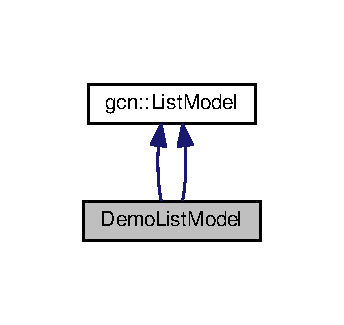
\includegraphics[width=165pt]{classDemoListModel__inherit__graph}
\end{center}
\end{figure}


Collaboration diagram for Demo\+List\+Model\+:\nopagebreak
\begin{figure}[H]
\begin{center}
\leavevmode
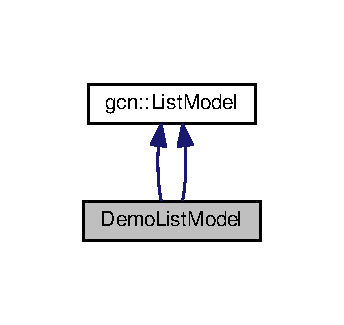
\includegraphics[width=165pt]{classDemoListModel__coll__graph}
\end{center}
\end{figure}
\subsection*{Public Member Functions}
\begin{DoxyCompactItemize}
\item 
int \hyperlink{classDemoListModel_a117af5914b15d9e2ed8350017a6e7b87}{get\+Number\+Of\+Elements} ()
\item 
std\+::string \hyperlink{classDemoListModel_a7df8cb4e14e5cf7b8859e91ab97ba8e7}{get\+Element\+At} (int i)
\item 
int \hyperlink{classDemoListModel_a117af5914b15d9e2ed8350017a6e7b87}{get\+Number\+Of\+Elements} ()
\item 
std\+::string \hyperlink{classDemoListModel_a7df8cb4e14e5cf7b8859e91ab97ba8e7}{get\+Element\+At} (int i)
\end{DoxyCompactItemize}


\subsection{Member Function Documentation}
\index{Demo\+List\+Model@{Demo\+List\+Model}!get\+Element\+At@{get\+Element\+At}}
\index{get\+Element\+At@{get\+Element\+At}!Demo\+List\+Model@{Demo\+List\+Model}}
\subsubsection[{\texorpdfstring{get\+Element\+At(int i)}{getElementAt(int i)}}]{\setlength{\rightskip}{0pt plus 5cm}std\+::string Demo\+List\+Model\+::get\+Element\+At (
\begin{DoxyParamCaption}
\item[{int}]{i}
\end{DoxyParamCaption}
)\hspace{0.3cm}{\ttfamily [inline]}, {\ttfamily [virtual]}}\hypertarget{classDemoListModel_a7df8cb4e14e5cf7b8859e91ab97ba8e7}{}\label{classDemoListModel_a7df8cb4e14e5cf7b8859e91ab97ba8e7}
Gets an element at a certain index in the list.


\begin{DoxyParams}{Parameters}
{\em i} & an index in the list. \\
\hline
\end{DoxyParams}
\begin{DoxyReturn}{Returns}
an element as a string. 
\end{DoxyReturn}


Implements \hyperlink{classgcn_1_1ListModel_a60c9432c539666c3e2ac6a2bee91e87f}{gcn\+::\+List\+Model}.

\index{Demo\+List\+Model@{Demo\+List\+Model}!get\+Element\+At@{get\+Element\+At}}
\index{get\+Element\+At@{get\+Element\+At}!Demo\+List\+Model@{Demo\+List\+Model}}
\subsubsection[{\texorpdfstring{get\+Element\+At(int i)}{getElementAt(int i)}}]{\setlength{\rightskip}{0pt plus 5cm}std\+::string Demo\+List\+Model\+::get\+Element\+At (
\begin{DoxyParamCaption}
\item[{int}]{i}
\end{DoxyParamCaption}
)\hspace{0.3cm}{\ttfamily [inline]}, {\ttfamily [virtual]}}\hypertarget{classDemoListModel_a7df8cb4e14e5cf7b8859e91ab97ba8e7}{}\label{classDemoListModel_a7df8cb4e14e5cf7b8859e91ab97ba8e7}
Gets an element at a certain index in the list.


\begin{DoxyParams}{Parameters}
{\em i} & an index in the list. \\
\hline
\end{DoxyParams}
\begin{DoxyReturn}{Returns}
an element as a string. 
\end{DoxyReturn}


Implements \hyperlink{classgcn_1_1ListModel_a60c9432c539666c3e2ac6a2bee91e87f}{gcn\+::\+List\+Model}.

\index{Demo\+List\+Model@{Demo\+List\+Model}!get\+Number\+Of\+Elements@{get\+Number\+Of\+Elements}}
\index{get\+Number\+Of\+Elements@{get\+Number\+Of\+Elements}!Demo\+List\+Model@{Demo\+List\+Model}}
\subsubsection[{\texorpdfstring{get\+Number\+Of\+Elements()}{getNumberOfElements()}}]{\setlength{\rightskip}{0pt plus 5cm}int Demo\+List\+Model\+::get\+Number\+Of\+Elements (
\begin{DoxyParamCaption}
{}
\end{DoxyParamCaption}
)\hspace{0.3cm}{\ttfamily [inline]}, {\ttfamily [virtual]}}\hypertarget{classDemoListModel_a117af5914b15d9e2ed8350017a6e7b87}{}\label{classDemoListModel_a117af5914b15d9e2ed8350017a6e7b87}
Gets the number of elements in the List\+Model.

\begin{DoxyReturn}{Returns}
the number of elements in the List\+Model 
\end{DoxyReturn}


Implements \hyperlink{classgcn_1_1ListModel_afc92c70252b9888f22b0164bc28f452c}{gcn\+::\+List\+Model}.

\index{Demo\+List\+Model@{Demo\+List\+Model}!get\+Number\+Of\+Elements@{get\+Number\+Of\+Elements}}
\index{get\+Number\+Of\+Elements@{get\+Number\+Of\+Elements}!Demo\+List\+Model@{Demo\+List\+Model}}
\subsubsection[{\texorpdfstring{get\+Number\+Of\+Elements()}{getNumberOfElements()}}]{\setlength{\rightskip}{0pt plus 5cm}int Demo\+List\+Model\+::get\+Number\+Of\+Elements (
\begin{DoxyParamCaption}
{}
\end{DoxyParamCaption}
)\hspace{0.3cm}{\ttfamily [inline]}, {\ttfamily [virtual]}}\hypertarget{classDemoListModel_a117af5914b15d9e2ed8350017a6e7b87}{}\label{classDemoListModel_a117af5914b15d9e2ed8350017a6e7b87}
Gets the number of elements in the List\+Model.

\begin{DoxyReturn}{Returns}
the number of elements in the List\+Model 
\end{DoxyReturn}


Implements \hyperlink{classgcn_1_1ListModel_afc92c70252b9888f22b0164bc28f452c}{gcn\+::\+List\+Model}.



The documentation for this class was generated from the following files\+:\begin{DoxyCompactItemize}
\item 
examples/openglwidgets.\+cpp\item 
examples/sdlwidgets.\+cpp\end{DoxyCompactItemize}

\hypertarget{classgcn_1_1DropDown}{}\section{gcn\+:\+:Drop\+Down Class Reference}
\label{classgcn_1_1DropDown}\index{gcn\+::\+Drop\+Down@{gcn\+::\+Drop\+Down}}


{\ttfamily \#include $<$dropdown.\+hpp$>$}



Inheritance diagram for gcn\+:\+:Drop\+Down\+:\nopagebreak
\begin{figure}[H]
\begin{center}
\leavevmode
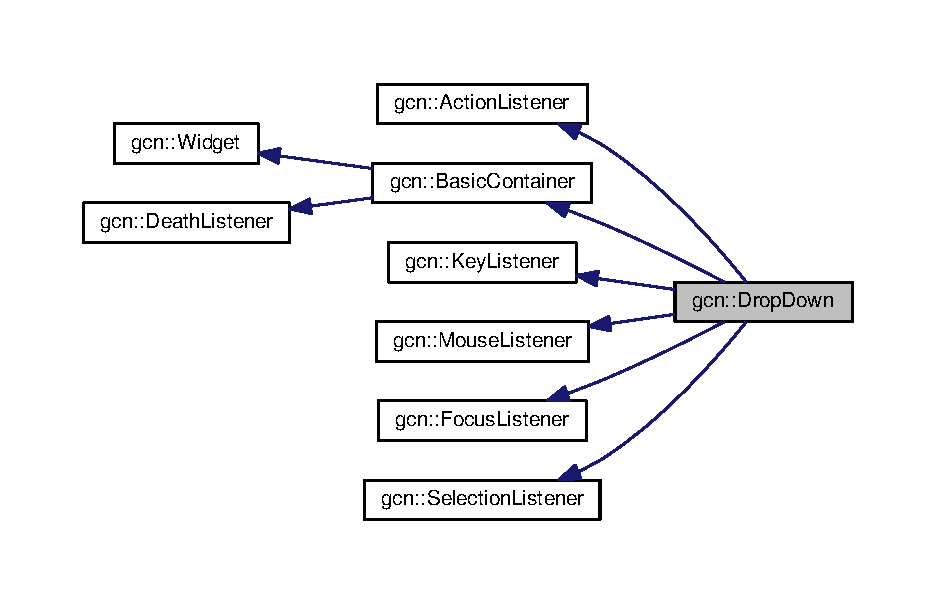
\includegraphics[width=350pt]{classgcn_1_1DropDown__inherit__graph}
\end{center}
\end{figure}


Collaboration diagram for gcn\+:\+:Drop\+Down\+:\nopagebreak
\begin{figure}[H]
\begin{center}
\leavevmode
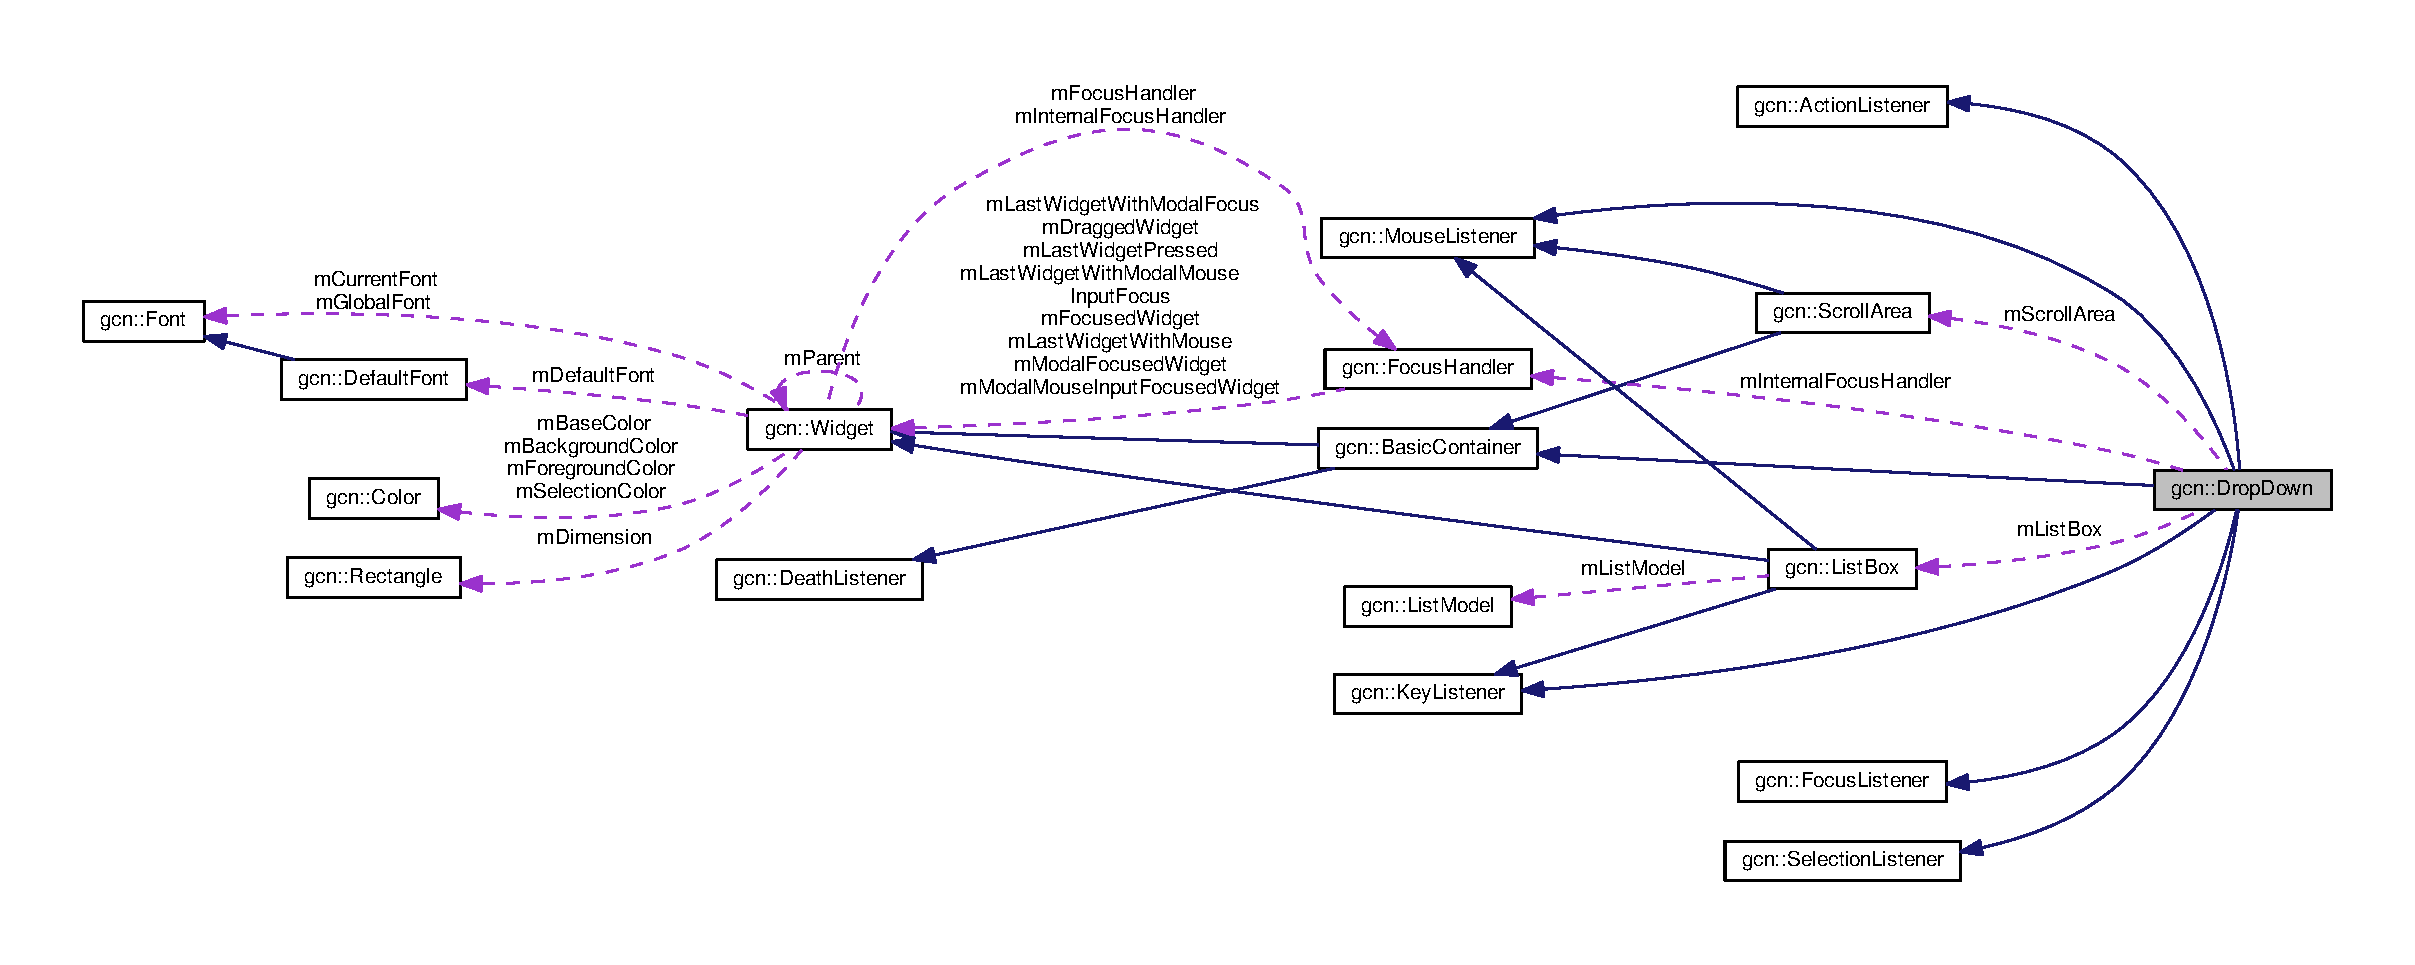
\includegraphics[width=350pt]{classgcn_1_1DropDown__coll__graph}
\end{center}
\end{figure}
\subsection*{Public Member Functions}
\begin{DoxyCompactItemize}
\item 
\hyperlink{classgcn_1_1DropDown_a8cc1eaa43f21818e6a80606ce5543099}{Drop\+Down} (\hyperlink{classgcn_1_1ListModel}{List\+Model} $\ast$list\+Model=N\+U\+LL, \hyperlink{classgcn_1_1ScrollArea}{Scroll\+Area} $\ast$scroll\+Area=N\+U\+LL, \hyperlink{classgcn_1_1ListBox}{List\+Box} $\ast$list\+Box=N\+U\+LL)
\item 
virtual \hyperlink{classgcn_1_1DropDown_afd2801677bd40fabb3dba5e28758fdf0}{$\sim$\+Drop\+Down} ()
\item 
int \hyperlink{classgcn_1_1DropDown_aeefe59776b354441faa9cc396723e905}{get\+Selected} () const 
\item 
void \hyperlink{classgcn_1_1DropDown_a01042c330073ed25d7ec4629647bdf79}{set\+Selected} (int selected)
\item 
void \hyperlink{classgcn_1_1DropDown_adc12528be39ab01791c71969a00e37c2}{set\+List\+Model} (\hyperlink{classgcn_1_1ListModel}{List\+Model} $\ast$list\+Model)
\item 
\hyperlink{classgcn_1_1ListModel}{List\+Model} $\ast$ \hyperlink{classgcn_1_1DropDown_a3c2ab20b50c9421accb76b557e558054}{get\+List\+Model} ()
\item 
void \hyperlink{classgcn_1_1DropDown_a39f06966d6236c7ead1a32c121dabcf9}{adjust\+Height} ()
\item 
void \hyperlink{classgcn_1_1DropDown_a82a8e42e1a902e32e7d2917665039073}{add\+Selection\+Listener} (\hyperlink{classgcn_1_1SelectionListener}{Selection\+Listener} $\ast$selection\+Listener)
\item 
void \hyperlink{classgcn_1_1DropDown_a44a2e345d02a70417398cbe52b6d3495}{remove\+Selection\+Listener} (\hyperlink{classgcn_1_1SelectionListener}{Selection\+Listener} $\ast$selection\+Listener)
\item 
virtual void \hyperlink{classgcn_1_1DropDown_acf081df400b8dd2affac734122bfdc8c}{draw} (\hyperlink{classgcn_1_1Graphics}{Graphics} $\ast$graphics)
\item 
virtual void \hyperlink{classgcn_1_1DropDown_a0fd541dd030eab962d27c1488f0d0aac}{draw\+Border} (\hyperlink{classgcn_1_1Graphics}{Graphics} $\ast$graphics)
\item 
void {\bfseries set\+Base\+Color} (const \hyperlink{classgcn_1_1Color}{Color} \&color)\hypertarget{classgcn_1_1DropDown_a2544d55f5bae9b499b2d29c8d0cf0ca6}{}\label{classgcn_1_1DropDown_a2544d55f5bae9b499b2d29c8d0cf0ca6}

\item 
void {\bfseries set\+Background\+Color} (const \hyperlink{classgcn_1_1Color}{Color} \&color)\hypertarget{classgcn_1_1DropDown_ad6b921be74f7825f5370efe4ab6700ed}{}\label{classgcn_1_1DropDown_ad6b921be74f7825f5370efe4ab6700ed}

\item 
void {\bfseries set\+Foreground\+Color} (const \hyperlink{classgcn_1_1Color}{Color} \&color)\hypertarget{classgcn_1_1DropDown_ab46dc804aab38d01a88ece5abb595261}{}\label{classgcn_1_1DropDown_ab46dc804aab38d01a88ece5abb595261}

\item 
void {\bfseries set\+Font} (\hyperlink{classgcn_1_1Font}{Font} $\ast$font)\hypertarget{classgcn_1_1DropDown_accdcc834a12cd77ad74776606bf7dc50}{}\label{classgcn_1_1DropDown_accdcc834a12cd77ad74776606bf7dc50}

\item 
void {\bfseries set\+Selection\+Color} (const \hyperlink{classgcn_1_1Color}{Color} \&color)\hypertarget{classgcn_1_1DropDown_a665aa223952505b6e974b762d0c49866}{}\label{classgcn_1_1DropDown_a665aa223952505b6e974b762d0c49866}

\item 
virtual \hyperlink{classgcn_1_1Rectangle}{Rectangle} \hyperlink{classgcn_1_1DropDown_ad61f89e8985a3a3be217dd15e199633d}{get\+Children\+Area} ()
\item 
virtual void \hyperlink{classgcn_1_1DropDown_a688cf78090ce646ea35e1ca00a441b12}{focus\+Lost} (const \hyperlink{classgcn_1_1Event}{Event} \&event)
\item 
virtual void \hyperlink{classgcn_1_1DropDown_aed63325d931d3d9d3df7400bd3b89f3e}{action} (const \hyperlink{classgcn_1_1ActionEvent}{Action\+Event} \&action\+Event)
\item 
virtual void \hyperlink{classgcn_1_1DropDown_a8f6402e1ad3ac77b7db296bbd77a7494}{death} (const \hyperlink{classgcn_1_1Event}{Event} \&event)
\item 
virtual void \hyperlink{classgcn_1_1DropDown_a10e7ba776f5c93185c9c8a18b9c3bfa6}{key\+Pressed} (\hyperlink{classgcn_1_1KeyEvent}{Key\+Event} \&key\+Event)
\item 
virtual void \hyperlink{classgcn_1_1DropDown_a3865e886c7e7f475d49dbae1772805e9}{mouse\+Pressed} (\hyperlink{classgcn_1_1MouseEvent}{Mouse\+Event} \&mouse\+Event)
\item 
virtual void \hyperlink{classgcn_1_1DropDown_ac62161f8fc0cfb09d901a9376ae8d416}{mouse\+Released} (\hyperlink{classgcn_1_1MouseEvent}{Mouse\+Event} \&mouse\+Event)
\item 
virtual void \hyperlink{classgcn_1_1DropDown_aaee24c3f98bff6165b4fff5fd0a433c1}{mouse\+Wheel\+Moved\+Up} (\hyperlink{classgcn_1_1MouseEvent}{Mouse\+Event} \&mouse\+Event)
\item 
virtual void \hyperlink{classgcn_1_1DropDown_ae84a6afe8d813f32cafbf774eebae6b2}{mouse\+Wheel\+Moved\+Down} (\hyperlink{classgcn_1_1MouseEvent}{Mouse\+Event} \&mouse\+Event)
\item 
virtual void \hyperlink{classgcn_1_1DropDown_a1cef091cc5cf19aa64171276e787ad72}{mouse\+Dragged} (\hyperlink{classgcn_1_1MouseEvent}{Mouse\+Event} \&mouse\+Event)
\item 
virtual void \hyperlink{classgcn_1_1DropDown_a76129029923e0c520b1ade9f242c09e3}{value\+Changed} (const \hyperlink{classgcn_1_1SelectionEvent}{Selection\+Event} \&event)
\end{DoxyCompactItemize}
\subsection*{Protected Types}
\begin{DoxyCompactItemize}
\item 
typedef std\+::list$<$ \hyperlink{classgcn_1_1SelectionListener}{Selection\+Listener} $\ast$ $>$ \hyperlink{classgcn_1_1DropDown_a04c257fcc8360fdff851c66a8ada149e}{Selection\+Listener\+List}
\item 
typedef Selection\+Listener\+List\+::iterator \hyperlink{classgcn_1_1DropDown_a836c8426a53976c1fbecad118ae72ea7}{Selection\+Listener\+Iterator}
\end{DoxyCompactItemize}
\subsection*{Protected Member Functions}
\begin{DoxyCompactItemize}
\item 
virtual void \hyperlink{classgcn_1_1DropDown_ae4dd73bd704e8801d25e858a19a5e5e4}{draw\+Button} (\hyperlink{classgcn_1_1Graphics}{Graphics} $\ast$graphics)
\item 
virtual void \hyperlink{classgcn_1_1DropDown_aa26df3e489e7982446381c782578bbbb}{drop\+Down} ()
\item 
virtual void \hyperlink{classgcn_1_1DropDown_a6fa979a9064a33f72f4bc7ca6733fe69}{fold\+Up} ()
\item 
void \hyperlink{classgcn_1_1DropDown_abbb9a251110710fa2af114476c6a4c23}{distribute\+Value\+Changed\+Event} ()
\end{DoxyCompactItemize}
\subsection*{Protected Attributes}
\begin{DoxyCompactItemize}
\item 
bool {\bfseries m\+Dropped\+Down}\hypertarget{classgcn_1_1DropDown_a6044d9242a012940b40f82aca990f1b1}{}\label{classgcn_1_1DropDown_a6044d9242a012940b40f82aca990f1b1}

\item 
bool {\bfseries m\+Pushed}\hypertarget{classgcn_1_1DropDown_af2be6c53414e75bed1f7c26a04c162cd}{}\label{classgcn_1_1DropDown_af2be6c53414e75bed1f7c26a04c162cd}

\item 
int \hyperlink{classgcn_1_1DropDown_a19582187e93e0c963ce131e4dda76ed0}{m\+Folded\+Up\+Height}
\item 
\hyperlink{classgcn_1_1ScrollArea}{Scroll\+Area} $\ast$ \hyperlink{classgcn_1_1DropDown_ad993ee12246ec45ae933dc0b69120858}{m\+Scroll\+Area}
\item 
\hyperlink{classgcn_1_1ListBox}{List\+Box} $\ast$ {\bfseries m\+List\+Box}\hypertarget{classgcn_1_1DropDown_a1931b17ba473552e48df708af1e4981b}{}\label{classgcn_1_1DropDown_a1931b17ba473552e48df708af1e4981b}

\item 
\hyperlink{classgcn_1_1FocusHandler}{Focus\+Handler} {\bfseries m\+Internal\+Focus\+Handler}\hypertarget{classgcn_1_1DropDown_a53e3e591e6d368f4a51f8879d4f56873}{}\label{classgcn_1_1DropDown_a53e3e591e6d368f4a51f8879d4f56873}

\item 
bool {\bfseries m\+Internal\+Scroll\+Area}\hypertarget{classgcn_1_1DropDown_afa6235ad0b7181c6d6e6c0f20de2df3d}{}\label{classgcn_1_1DropDown_afa6235ad0b7181c6d6e6c0f20de2df3d}

\item 
bool {\bfseries m\+Internal\+List\+Box}\hypertarget{classgcn_1_1DropDown_ab77b80e2db20ca032c2e51fec24929b9}{}\label{classgcn_1_1DropDown_ab77b80e2db20ca032c2e51fec24929b9}

\item 
bool {\bfseries m\+Is\+Dragged}\hypertarget{classgcn_1_1DropDown_a1360f37268fac8557b8711d299315e84}{}\label{classgcn_1_1DropDown_a1360f37268fac8557b8711d299315e84}

\item 
\hyperlink{classgcn_1_1DropDown_a04c257fcc8360fdff851c66a8ada149e}{Selection\+Listener\+List} \hyperlink{classgcn_1_1DropDown_af75c84f875796ada546de4ee008f165e}{m\+Selection\+Listeners}
\end{DoxyCompactItemize}
\subsection*{Additional Inherited Members}


\subsection{Detailed Description}
An implementation of a drop downable list from which an item can be selected. The drop down consists of an internal \hyperlink{classgcn_1_1ScrollArea}{Scroll\+Area} and an internal \hyperlink{classgcn_1_1ListBox}{List\+Box}. The drop down also uses an internal \hyperlink{classgcn_1_1FocusHandler}{Focus\+Handler} to handle the focus of the internal Scoll\+Area and the internal \hyperlink{classgcn_1_1ListBox}{List\+Box}. The scroll area and the list box can be passed to the drop down if a custom scroll area and or a custom list box is preferable.

To be able display a list the drop down uses a user provided list model. A list model can be any class that implements the \hyperlink{classgcn_1_1ListModel}{List\+Model} interface.

If an item is selected in the drop down a select event will be sent to all selection listeners of the drop down. If an item is selected by using a mouse click or by using the enter or space key an action event will be sent to all action listeners of the drop down. 

\subsection{Member Typedef Documentation}
\index{gcn\+::\+Drop\+Down@{gcn\+::\+Drop\+Down}!Selection\+Listener\+Iterator@{Selection\+Listener\+Iterator}}
\index{Selection\+Listener\+Iterator@{Selection\+Listener\+Iterator}!gcn\+::\+Drop\+Down@{gcn\+::\+Drop\+Down}}
\subsubsection[{\texorpdfstring{Selection\+Listener\+Iterator}{SelectionListenerIterator}}]{\setlength{\rightskip}{0pt plus 5cm}typedef Selection\+Listener\+List\+::iterator {\bf gcn\+::\+Drop\+Down\+::\+Selection\+Listener\+Iterator}\hspace{0.3cm}{\ttfamily [protected]}}\hypertarget{classgcn_1_1DropDown_a836c8426a53976c1fbecad118ae72ea7}{}\label{classgcn_1_1DropDown_a836c8426a53976c1fbecad118ae72ea7}
Typedef. \index{gcn\+::\+Drop\+Down@{gcn\+::\+Drop\+Down}!Selection\+Listener\+List@{Selection\+Listener\+List}}
\index{Selection\+Listener\+List@{Selection\+Listener\+List}!gcn\+::\+Drop\+Down@{gcn\+::\+Drop\+Down}}
\subsubsection[{\texorpdfstring{Selection\+Listener\+List}{SelectionListenerList}}]{\setlength{\rightskip}{0pt plus 5cm}typedef std\+::list$<${\bf Selection\+Listener}$\ast$$>$ {\bf gcn\+::\+Drop\+Down\+::\+Selection\+Listener\+List}\hspace{0.3cm}{\ttfamily [protected]}}\hypertarget{classgcn_1_1DropDown_a04c257fcc8360fdff851c66a8ada149e}{}\label{classgcn_1_1DropDown_a04c257fcc8360fdff851c66a8ada149e}
Typedef. 

\subsection{Constructor \& Destructor Documentation}
\index{gcn\+::\+Drop\+Down@{gcn\+::\+Drop\+Down}!Drop\+Down@{Drop\+Down}}
\index{Drop\+Down@{Drop\+Down}!gcn\+::\+Drop\+Down@{gcn\+::\+Drop\+Down}}
\subsubsection[{\texorpdfstring{Drop\+Down(\+List\+Model $\ast$list\+Model=\+N\+U\+L\+L, Scroll\+Area $\ast$scroll\+Area=\+N\+U\+L\+L, List\+Box $\ast$list\+Box=\+N\+U\+L\+L)}{DropDown(ListModel *listModel=NULL, ScrollArea *scrollArea=NULL, ListBox *listBox=NULL)}}]{\setlength{\rightskip}{0pt plus 5cm}gcn\+::\+Drop\+Down\+::\+Drop\+Down (
\begin{DoxyParamCaption}
\item[{{\bf List\+Model} $\ast$}]{list\+Model = {\ttfamily NULL}, }
\item[{{\bf Scroll\+Area} $\ast$}]{scroll\+Area = {\ttfamily NULL}, }
\item[{{\bf List\+Box} $\ast$}]{list\+Box = {\ttfamily NULL}}
\end{DoxyParamCaption}
)}\hypertarget{classgcn_1_1DropDown_a8cc1eaa43f21818e6a80606ce5543099}{}\label{classgcn_1_1DropDown_a8cc1eaa43f21818e6a80606ce5543099}
Contructor.


\begin{DoxyParams}{Parameters}
{\em list\+Model} & the \hyperlink{classgcn_1_1ListModel}{List\+Model} to use. \\
\hline
{\em scroll\+Area} & the \hyperlink{classgcn_1_1ScrollArea}{Scroll\+Area} to use. \\
\hline
{\em list\+Box} & the list\+Box to use. \\
\hline
\end{DoxyParams}
\begin{DoxySeeAlso}{See also}
\hyperlink{classgcn_1_1ListModel}{List\+Model}, \hyperlink{classgcn_1_1ScrollArea}{Scroll\+Area}, \hyperlink{classgcn_1_1ListBox}{List\+Box}. 
\end{DoxySeeAlso}
\index{gcn\+::\+Drop\+Down@{gcn\+::\+Drop\+Down}!````~Drop\+Down@{$\sim$\+Drop\+Down}}
\index{````~Drop\+Down@{$\sim$\+Drop\+Down}!gcn\+::\+Drop\+Down@{gcn\+::\+Drop\+Down}}
\subsubsection[{\texorpdfstring{$\sim$\+Drop\+Down()}{~DropDown()}}]{\setlength{\rightskip}{0pt plus 5cm}gcn\+::\+Drop\+Down\+::$\sim$\+Drop\+Down (
\begin{DoxyParamCaption}
{}
\end{DoxyParamCaption}
)\hspace{0.3cm}{\ttfamily [virtual]}}\hypertarget{classgcn_1_1DropDown_afd2801677bd40fabb3dba5e28758fdf0}{}\label{classgcn_1_1DropDown_afd2801677bd40fabb3dba5e28758fdf0}
Destructor. 

\subsection{Member Function Documentation}
\index{gcn\+::\+Drop\+Down@{gcn\+::\+Drop\+Down}!action@{action}}
\index{action@{action}!gcn\+::\+Drop\+Down@{gcn\+::\+Drop\+Down}}
\subsubsection[{\texorpdfstring{action(const Action\+Event \&action\+Event)}{action(const ActionEvent &actionEvent)}}]{\setlength{\rightskip}{0pt plus 5cm}void gcn\+::\+Drop\+Down\+::action (
\begin{DoxyParamCaption}
\item[{const {\bf Action\+Event} \&}]{action\+Event}
\end{DoxyParamCaption}
)\hspace{0.3cm}{\ttfamily [virtual]}}\hypertarget{classgcn_1_1DropDown_aed63325d931d3d9d3df7400bd3b89f3e}{}\label{classgcn_1_1DropDown_aed63325d931d3d9d3df7400bd3b89f3e}
Called when an action is recieved from a \hyperlink{classgcn_1_1Widget}{Widget}. It is used to be able to recieve a notification that an action has occured.


\begin{DoxyParams}{Parameters}
{\em action\+Event} & the event of the action. \\
\hline
\end{DoxyParams}
\begin{DoxySince}{Since}
0.\+6.\+0 
\end{DoxySince}


Implements \hyperlink{classgcn_1_1ActionListener_ae883112ab054a8589b5d82c47763a31d}{gcn\+::\+Action\+Listener}.

\index{gcn\+::\+Drop\+Down@{gcn\+::\+Drop\+Down}!add\+Selection\+Listener@{add\+Selection\+Listener}}
\index{add\+Selection\+Listener@{add\+Selection\+Listener}!gcn\+::\+Drop\+Down@{gcn\+::\+Drop\+Down}}
\subsubsection[{\texorpdfstring{add\+Selection\+Listener(\+Selection\+Listener $\ast$selection\+Listener)}{addSelectionListener(SelectionListener *selectionListener)}}]{\setlength{\rightskip}{0pt plus 5cm}void gcn\+::\+Drop\+Down\+::add\+Selection\+Listener (
\begin{DoxyParamCaption}
\item[{{\bf Selection\+Listener} $\ast$}]{selection\+Listener}
\end{DoxyParamCaption}
)}\hypertarget{classgcn_1_1DropDown_a82a8e42e1a902e32e7d2917665039073}{}\label{classgcn_1_1DropDown_a82a8e42e1a902e32e7d2917665039073}
Adds a selection listener to the drop down. When the selection changes an event will be sent to all selection listeners of the drop down.


\begin{DoxyParams}{Parameters}
{\em selection\+Listener} & the selection listener to add. \\
\hline
\end{DoxyParams}
\begin{DoxySince}{Since}
0.\+8.\+0 
\end{DoxySince}
\index{gcn\+::\+Drop\+Down@{gcn\+::\+Drop\+Down}!adjust\+Height@{adjust\+Height}}
\index{adjust\+Height@{adjust\+Height}!gcn\+::\+Drop\+Down@{gcn\+::\+Drop\+Down}}
\subsubsection[{\texorpdfstring{adjust\+Height()}{adjustHeight()}}]{\setlength{\rightskip}{0pt plus 5cm}void gcn\+::\+Drop\+Down\+::adjust\+Height (
\begin{DoxyParamCaption}
{}
\end{DoxyParamCaption}
)}\hypertarget{classgcn_1_1DropDown_a39f06966d6236c7ead1a32c121dabcf9}{}\label{classgcn_1_1DropDown_a39f06966d6236c7ead1a32c121dabcf9}
Adjusts the height of the drop down to fit the height of the drop down\textquotesingle{}s parent\textquotesingle{}s height. It\textquotesingle{}s used to not make the drop down draw itself outside of it\textquotesingle{}s parent if folded down. \index{gcn\+::\+Drop\+Down@{gcn\+::\+Drop\+Down}!death@{death}}
\index{death@{death}!gcn\+::\+Drop\+Down@{gcn\+::\+Drop\+Down}}
\subsubsection[{\texorpdfstring{death(const Event \&event)}{death(const Event &event)}}]{\setlength{\rightskip}{0pt plus 5cm}void gcn\+::\+Drop\+Down\+::death (
\begin{DoxyParamCaption}
\item[{const {\bf Event} \&}]{event}
\end{DoxyParamCaption}
)\hspace{0.3cm}{\ttfamily [virtual]}}\hypertarget{classgcn_1_1DropDown_a8f6402e1ad3ac77b7db296bbd77a7494}{}\label{classgcn_1_1DropDown_a8f6402e1ad3ac77b7db296bbd77a7494}
Called when a widget dies. It is used to be able to recieve a notification when a death of a widget occurs.


\begin{DoxyParams}{Parameters}
{\em event} & the event of the death. \\
\hline
\end{DoxyParams}


Reimplemented from \hyperlink{classgcn_1_1BasicContainer_ac6cf8760537dcd167e0f518f556bccf4}{gcn\+::\+Basic\+Container}.

\index{gcn\+::\+Drop\+Down@{gcn\+::\+Drop\+Down}!distribute\+Value\+Changed\+Event@{distribute\+Value\+Changed\+Event}}
\index{distribute\+Value\+Changed\+Event@{distribute\+Value\+Changed\+Event}!gcn\+::\+Drop\+Down@{gcn\+::\+Drop\+Down}}
\subsubsection[{\texorpdfstring{distribute\+Value\+Changed\+Event()}{distributeValueChangedEvent()}}]{\setlength{\rightskip}{0pt plus 5cm}void gcn\+::\+Drop\+Down\+::distribute\+Value\+Changed\+Event (
\begin{DoxyParamCaption}
{}
\end{DoxyParamCaption}
)\hspace{0.3cm}{\ttfamily [protected]}}\hypertarget{classgcn_1_1DropDown_abbb9a251110710fa2af114476c6a4c23}{}\label{classgcn_1_1DropDown_abbb9a251110710fa2af114476c6a4c23}
Distributes a value changed event to all selection listeners of the drop down.

\begin{DoxySince}{Since}
0.\+8.\+0 
\end{DoxySince}
\index{gcn\+::\+Drop\+Down@{gcn\+::\+Drop\+Down}!draw@{draw}}
\index{draw@{draw}!gcn\+::\+Drop\+Down@{gcn\+::\+Drop\+Down}}
\subsubsection[{\texorpdfstring{draw(\+Graphics $\ast$graphics)}{draw(Graphics *graphics)}}]{\setlength{\rightskip}{0pt plus 5cm}void gcn\+::\+Drop\+Down\+::draw (
\begin{DoxyParamCaption}
\item[{{\bf Graphics} $\ast$}]{graphics}
\end{DoxyParamCaption}
)\hspace{0.3cm}{\ttfamily [virtual]}}\hypertarget{classgcn_1_1DropDown_acf081df400b8dd2affac734122bfdc8c}{}\label{classgcn_1_1DropDown_acf081df400b8dd2affac734122bfdc8c}
Draws the widget. It is called by the parent widget when it is time for the widget to draw itself. The graphics object is set up so that all drawing is relative to the widget, i.\+e coordinate (0,0) is the top-\/left corner of the widget. It is not possible to draw outside of a widgets dimension.


\begin{DoxyParams}{Parameters}
{\em graphics} & a \hyperlink{classgcn_1_1Graphics}{Graphics} object to draw with. \\
\hline
\end{DoxyParams}


Implements \hyperlink{classgcn_1_1Widget_acc595221d6a2d1afe1043c16dc37d212}{gcn\+::\+Widget}.

\index{gcn\+::\+Drop\+Down@{gcn\+::\+Drop\+Down}!draw\+Border@{draw\+Border}}
\index{draw\+Border@{draw\+Border}!gcn\+::\+Drop\+Down@{gcn\+::\+Drop\+Down}}
\subsubsection[{\texorpdfstring{draw\+Border(\+Graphics $\ast$graphics)}{drawBorder(Graphics *graphics)}}]{\setlength{\rightskip}{0pt plus 5cm}void gcn\+::\+Drop\+Down\+::draw\+Border (
\begin{DoxyParamCaption}
\item[{{\bf Graphics} $\ast$}]{graphics}
\end{DoxyParamCaption}
)\hspace{0.3cm}{\ttfamily [virtual]}}\hypertarget{classgcn_1_1DropDown_a0fd541dd030eab962d27c1488f0d0aac}{}\label{classgcn_1_1DropDown_a0fd541dd030eab962d27c1488f0d0aac}
Draws the widget border. A border is drawn around a widget. The width and height of the border is therefore the widgets height+2$\ast$bordersize. Think of a painting that has a certain size, the border surrounds the painting.


\begin{DoxyParams}{Parameters}
{\em graphics} & a \hyperlink{classgcn_1_1Graphics}{Graphics} object to draw with. \\
\hline
\end{DoxyParams}


Reimplemented from \hyperlink{classgcn_1_1Widget_a58c3b2f513d8e029e321fd88a974f5c4}{gcn\+::\+Widget}.

\index{gcn\+::\+Drop\+Down@{gcn\+::\+Drop\+Down}!draw\+Button@{draw\+Button}}
\index{draw\+Button@{draw\+Button}!gcn\+::\+Drop\+Down@{gcn\+::\+Drop\+Down}}
\subsubsection[{\texorpdfstring{draw\+Button(\+Graphics $\ast$graphics)}{drawButton(Graphics *graphics)}}]{\setlength{\rightskip}{0pt plus 5cm}void gcn\+::\+Drop\+Down\+::draw\+Button (
\begin{DoxyParamCaption}
\item[{{\bf Graphics} $\ast$}]{graphics}
\end{DoxyParamCaption}
)\hspace{0.3cm}{\ttfamily [protected]}, {\ttfamily [virtual]}}\hypertarget{classgcn_1_1DropDown_ae4dd73bd704e8801d25e858a19a5e5e4}{}\label{classgcn_1_1DropDown_ae4dd73bd704e8801d25e858a19a5e5e4}
Draws the button with the little down arrow.


\begin{DoxyParams}{Parameters}
{\em graphics} & a \hyperlink{classgcn_1_1Graphics}{Graphics} object to draw with. \\
\hline
\end{DoxyParams}
\index{gcn\+::\+Drop\+Down@{gcn\+::\+Drop\+Down}!drop\+Down@{drop\+Down}}
\index{drop\+Down@{drop\+Down}!gcn\+::\+Drop\+Down@{gcn\+::\+Drop\+Down}}
\subsubsection[{\texorpdfstring{drop\+Down()}{dropDown()}}]{\setlength{\rightskip}{0pt plus 5cm}void gcn\+::\+Drop\+Down\+::drop\+Down (
\begin{DoxyParamCaption}
{}
\end{DoxyParamCaption}
)\hspace{0.3cm}{\ttfamily [protected]}, {\ttfamily [virtual]}}\hypertarget{classgcn_1_1DropDown_aa26df3e489e7982446381c782578bbbb}{}\label{classgcn_1_1DropDown_aa26df3e489e7982446381c782578bbbb}
Sets the \hyperlink{classgcn_1_1DropDown}{Drop\+Down} \hyperlink{classgcn_1_1Widget}{Widget} to dropped-\/down mode. \index{gcn\+::\+Drop\+Down@{gcn\+::\+Drop\+Down}!focus\+Lost@{focus\+Lost}}
\index{focus\+Lost@{focus\+Lost}!gcn\+::\+Drop\+Down@{gcn\+::\+Drop\+Down}}
\subsubsection[{\texorpdfstring{focus\+Lost(const Event \&event)}{focusLost(const Event &event)}}]{\setlength{\rightskip}{0pt plus 5cm}void gcn\+::\+Drop\+Down\+::focus\+Lost (
\begin{DoxyParamCaption}
\item[{const {\bf Event} \&}]{event}
\end{DoxyParamCaption}
)\hspace{0.3cm}{\ttfamily [virtual]}}\hypertarget{classgcn_1_1DropDown_a688cf78090ce646ea35e1ca00a441b12}{}\label{classgcn_1_1DropDown_a688cf78090ce646ea35e1ca00a441b12}
Called when a widget loses focus.


\begin{DoxyParams}{Parameters}
{\em event} & discribes the event. \\
\hline
\end{DoxyParams}


Reimplemented from \hyperlink{classgcn_1_1FocusListener_a7523032b39888503179e8142d2433b45}{gcn\+::\+Focus\+Listener}.

\index{gcn\+::\+Drop\+Down@{gcn\+::\+Drop\+Down}!fold\+Up@{fold\+Up}}
\index{fold\+Up@{fold\+Up}!gcn\+::\+Drop\+Down@{gcn\+::\+Drop\+Down}}
\subsubsection[{\texorpdfstring{fold\+Up()}{foldUp()}}]{\setlength{\rightskip}{0pt plus 5cm}void gcn\+::\+Drop\+Down\+::fold\+Up (
\begin{DoxyParamCaption}
{}
\end{DoxyParamCaption}
)\hspace{0.3cm}{\ttfamily [protected]}, {\ttfamily [virtual]}}\hypertarget{classgcn_1_1DropDown_a6fa979a9064a33f72f4bc7ca6733fe69}{}\label{classgcn_1_1DropDown_a6fa979a9064a33f72f4bc7ca6733fe69}
Sets the \hyperlink{classgcn_1_1DropDown}{Drop\+Down} \hyperlink{classgcn_1_1Widget}{Widget} to folded-\/up mode. \index{gcn\+::\+Drop\+Down@{gcn\+::\+Drop\+Down}!get\+Children\+Area@{get\+Children\+Area}}
\index{get\+Children\+Area@{get\+Children\+Area}!gcn\+::\+Drop\+Down@{gcn\+::\+Drop\+Down}}
\subsubsection[{\texorpdfstring{get\+Children\+Area()}{getChildrenArea()}}]{\setlength{\rightskip}{0pt plus 5cm}{\bf Rectangle} gcn\+::\+Drop\+Down\+::get\+Children\+Area (
\begin{DoxyParamCaption}
{}
\end{DoxyParamCaption}
)\hspace{0.3cm}{\ttfamily [virtual]}}\hypertarget{classgcn_1_1DropDown_ad61f89e8985a3a3be217dd15e199633d}{}\label{classgcn_1_1DropDown_ad61f89e8985a3a3be217dd15e199633d}
Gets the subarea of the widget that the children occupy.

\begin{DoxyReturn}{Returns}
the subarea as a \hyperlink{classgcn_1_1Rectangle}{Rectangle}. 
\end{DoxyReturn}


Reimplemented from \hyperlink{classgcn_1_1BasicContainer_a8ed853146d726cb3bc5d109ad52203d6}{gcn\+::\+Basic\+Container}.

\index{gcn\+::\+Drop\+Down@{gcn\+::\+Drop\+Down}!get\+List\+Model@{get\+List\+Model}}
\index{get\+List\+Model@{get\+List\+Model}!gcn\+::\+Drop\+Down@{gcn\+::\+Drop\+Down}}
\subsubsection[{\texorpdfstring{get\+List\+Model()}{getListModel()}}]{\setlength{\rightskip}{0pt plus 5cm}{\bf List\+Model} $\ast$ gcn\+::\+Drop\+Down\+::get\+List\+Model (
\begin{DoxyParamCaption}
{}
\end{DoxyParamCaption}
)}\hypertarget{classgcn_1_1DropDown_a3c2ab20b50c9421accb76b557e558054}{}\label{classgcn_1_1DropDown_a3c2ab20b50c9421accb76b557e558054}
Gets the list model used.

\begin{DoxyReturn}{Returns}
the \hyperlink{classgcn_1_1ListModel}{List\+Model} used. 
\end{DoxyReturn}
\begin{DoxySeeAlso}{See also}
\hyperlink{classgcn_1_1DropDown_adc12528be39ab01791c71969a00e37c2}{set\+List\+Model} 
\end{DoxySeeAlso}
\index{gcn\+::\+Drop\+Down@{gcn\+::\+Drop\+Down}!get\+Selected@{get\+Selected}}
\index{get\+Selected@{get\+Selected}!gcn\+::\+Drop\+Down@{gcn\+::\+Drop\+Down}}
\subsubsection[{\texorpdfstring{get\+Selected() const }{getSelected() const }}]{\setlength{\rightskip}{0pt plus 5cm}int gcn\+::\+Drop\+Down\+::get\+Selected (
\begin{DoxyParamCaption}
{}
\end{DoxyParamCaption}
) const}\hypertarget{classgcn_1_1DropDown_aeefe59776b354441faa9cc396723e905}{}\label{classgcn_1_1DropDown_aeefe59776b354441faa9cc396723e905}
Gets the selected item as an index in the list model.

\begin{DoxyReturn}{Returns}
the selected item as an index in the list model. 
\end{DoxyReturn}
\begin{DoxySeeAlso}{See also}
\hyperlink{classgcn_1_1DropDown_a01042c330073ed25d7ec4629647bdf79}{set\+Selected} 
\end{DoxySeeAlso}
\index{gcn\+::\+Drop\+Down@{gcn\+::\+Drop\+Down}!key\+Pressed@{key\+Pressed}}
\index{key\+Pressed@{key\+Pressed}!gcn\+::\+Drop\+Down@{gcn\+::\+Drop\+Down}}
\subsubsection[{\texorpdfstring{key\+Pressed(\+Key\+Event \&key\+Event)}{keyPressed(KeyEvent &keyEvent)}}]{\setlength{\rightskip}{0pt plus 5cm}void gcn\+::\+Drop\+Down\+::key\+Pressed (
\begin{DoxyParamCaption}
\item[{{\bf Key\+Event} \&}]{key\+Event}
\end{DoxyParamCaption}
)\hspace{0.3cm}{\ttfamily [virtual]}}\hypertarget{classgcn_1_1DropDown_a10e7ba776f5c93185c9c8a18b9c3bfa6}{}\label{classgcn_1_1DropDown_a10e7ba776f5c93185c9c8a18b9c3bfa6}
Called if a key is pressed when the widget has keyboard focus. If a key is held down the widget will generate multiple key presses.


\begin{DoxyParams}{Parameters}
{\em key\+Event} & discribes the event. \\
\hline
\end{DoxyParams}


Reimplemented from \hyperlink{classgcn_1_1KeyListener_ada6c0d038340d6ee674702268b2d2c67}{gcn\+::\+Key\+Listener}.

\index{gcn\+::\+Drop\+Down@{gcn\+::\+Drop\+Down}!mouse\+Dragged@{mouse\+Dragged}}
\index{mouse\+Dragged@{mouse\+Dragged}!gcn\+::\+Drop\+Down@{gcn\+::\+Drop\+Down}}
\subsubsection[{\texorpdfstring{mouse\+Dragged(\+Mouse\+Event \&mouse\+Event)}{mouseDragged(MouseEvent &mouseEvent)}}]{\setlength{\rightskip}{0pt plus 5cm}void gcn\+::\+Drop\+Down\+::mouse\+Dragged (
\begin{DoxyParamCaption}
\item[{{\bf Mouse\+Event} \&}]{mouse\+Event}
\end{DoxyParamCaption}
)\hspace{0.3cm}{\ttfamily [virtual]}}\hypertarget{classgcn_1_1DropDown_a1cef091cc5cf19aa64171276e787ad72}{}\label{classgcn_1_1DropDown_a1cef091cc5cf19aa64171276e787ad72}
Called when the mouse has moved and the mouse has previously been pressed on the widget.


\begin{DoxyParams}{Parameters}
{\em mouse\+Event} & describes the event. \\
\hline
\end{DoxyParams}
\begin{DoxySince}{Since}
0.\+6.\+0 
\end{DoxySince}


Reimplemented from \hyperlink{classgcn_1_1MouseListener_a5e2764977dd75e52d116f9ba6311a46b}{gcn\+::\+Mouse\+Listener}.

\index{gcn\+::\+Drop\+Down@{gcn\+::\+Drop\+Down}!mouse\+Pressed@{mouse\+Pressed}}
\index{mouse\+Pressed@{mouse\+Pressed}!gcn\+::\+Drop\+Down@{gcn\+::\+Drop\+Down}}
\subsubsection[{\texorpdfstring{mouse\+Pressed(\+Mouse\+Event \&mouse\+Event)}{mousePressed(MouseEvent &mouseEvent)}}]{\setlength{\rightskip}{0pt plus 5cm}void gcn\+::\+Drop\+Down\+::mouse\+Pressed (
\begin{DoxyParamCaption}
\item[{{\bf Mouse\+Event} \&}]{mouse\+Event}
\end{DoxyParamCaption}
)\hspace{0.3cm}{\ttfamily [virtual]}}\hypertarget{classgcn_1_1DropDown_a3865e886c7e7f475d49dbae1772805e9}{}\label{classgcn_1_1DropDown_a3865e886c7e7f475d49dbae1772805e9}
Called when a mouse button has been pressed on the widget area.

N\+O\+TE\+: A mouse press is N\+OT equal to a mouse click. Use mouse\+Click\+Message to check for mouse clicks.


\begin{DoxyParams}{Parameters}
{\em mouse\+Event} & describes the event. \\
\hline
\end{DoxyParams}
\begin{DoxySince}{Since}
0.\+6.\+0 
\end{DoxySince}


Reimplemented from \hyperlink{classgcn_1_1MouseListener_af81ee6190a48a18585f6e738e381abd3}{gcn\+::\+Mouse\+Listener}.

\index{gcn\+::\+Drop\+Down@{gcn\+::\+Drop\+Down}!mouse\+Released@{mouse\+Released}}
\index{mouse\+Released@{mouse\+Released}!gcn\+::\+Drop\+Down@{gcn\+::\+Drop\+Down}}
\subsubsection[{\texorpdfstring{mouse\+Released(\+Mouse\+Event \&mouse\+Event)}{mouseReleased(MouseEvent &mouseEvent)}}]{\setlength{\rightskip}{0pt plus 5cm}void gcn\+::\+Drop\+Down\+::mouse\+Released (
\begin{DoxyParamCaption}
\item[{{\bf Mouse\+Event} \&}]{mouse\+Event}
\end{DoxyParamCaption}
)\hspace{0.3cm}{\ttfamily [virtual]}}\hypertarget{classgcn_1_1DropDown_ac62161f8fc0cfb09d901a9376ae8d416}{}\label{classgcn_1_1DropDown_ac62161f8fc0cfb09d901a9376ae8d416}
Called when a mouse button has been released on the widget area.


\begin{DoxyParams}{Parameters}
{\em mouse\+Event} & describes the event. \\
\hline
\end{DoxyParams}


Reimplemented from \hyperlink{classgcn_1_1MouseListener_adf68ed80e1a3c027fbb5d0e575b20fc3}{gcn\+::\+Mouse\+Listener}.

\index{gcn\+::\+Drop\+Down@{gcn\+::\+Drop\+Down}!mouse\+Wheel\+Moved\+Down@{mouse\+Wheel\+Moved\+Down}}
\index{mouse\+Wheel\+Moved\+Down@{mouse\+Wheel\+Moved\+Down}!gcn\+::\+Drop\+Down@{gcn\+::\+Drop\+Down}}
\subsubsection[{\texorpdfstring{mouse\+Wheel\+Moved\+Down(\+Mouse\+Event \&mouse\+Event)}{mouseWheelMovedDown(MouseEvent &mouseEvent)}}]{\setlength{\rightskip}{0pt plus 5cm}void gcn\+::\+Drop\+Down\+::mouse\+Wheel\+Moved\+Down (
\begin{DoxyParamCaption}
\item[{{\bf Mouse\+Event} \&}]{mouse\+Event}
\end{DoxyParamCaption}
)\hspace{0.3cm}{\ttfamily [virtual]}}\hypertarget{classgcn_1_1DropDown_ae84a6afe8d813f32cafbf774eebae6b2}{}\label{classgcn_1_1DropDown_ae84a6afe8d813f32cafbf774eebae6b2}
Called when the mouse wheel has moved down on the widget area.


\begin{DoxyParams}{Parameters}
{\em mous\+Event} & describes the event. \\
\hline
\end{DoxyParams}
\begin{DoxySince}{Since}
0.\+6.\+0 
\end{DoxySince}


Reimplemented from \hyperlink{classgcn_1_1MouseListener_ab177e069d747626bcf228149c4391320}{gcn\+::\+Mouse\+Listener}.

\index{gcn\+::\+Drop\+Down@{gcn\+::\+Drop\+Down}!mouse\+Wheel\+Moved\+Up@{mouse\+Wheel\+Moved\+Up}}
\index{mouse\+Wheel\+Moved\+Up@{mouse\+Wheel\+Moved\+Up}!gcn\+::\+Drop\+Down@{gcn\+::\+Drop\+Down}}
\subsubsection[{\texorpdfstring{mouse\+Wheel\+Moved\+Up(\+Mouse\+Event \&mouse\+Event)}{mouseWheelMovedUp(MouseEvent &mouseEvent)}}]{\setlength{\rightskip}{0pt plus 5cm}void gcn\+::\+Drop\+Down\+::mouse\+Wheel\+Moved\+Up (
\begin{DoxyParamCaption}
\item[{{\bf Mouse\+Event} \&}]{mouse\+Event}
\end{DoxyParamCaption}
)\hspace{0.3cm}{\ttfamily [virtual]}}\hypertarget{classgcn_1_1DropDown_aaee24c3f98bff6165b4fff5fd0a433c1}{}\label{classgcn_1_1DropDown_aaee24c3f98bff6165b4fff5fd0a433c1}
Called when the mouse wheel has moved up on the widget area.


\begin{DoxyParams}{Parameters}
{\em mouse\+Event} & describes the event. \\
\hline
\end{DoxyParams}
\begin{DoxySince}{Since}
0.\+6.\+0 
\end{DoxySince}


Reimplemented from \hyperlink{classgcn_1_1MouseListener_ab3cb0eb9b771656461d3e0248127721d}{gcn\+::\+Mouse\+Listener}.

\index{gcn\+::\+Drop\+Down@{gcn\+::\+Drop\+Down}!remove\+Selection\+Listener@{remove\+Selection\+Listener}}
\index{remove\+Selection\+Listener@{remove\+Selection\+Listener}!gcn\+::\+Drop\+Down@{gcn\+::\+Drop\+Down}}
\subsubsection[{\texorpdfstring{remove\+Selection\+Listener(\+Selection\+Listener $\ast$selection\+Listener)}{removeSelectionListener(SelectionListener *selectionListener)}}]{\setlength{\rightskip}{0pt plus 5cm}void gcn\+::\+Drop\+Down\+::remove\+Selection\+Listener (
\begin{DoxyParamCaption}
\item[{{\bf Selection\+Listener} $\ast$}]{selection\+Listener}
\end{DoxyParamCaption}
)}\hypertarget{classgcn_1_1DropDown_a44a2e345d02a70417398cbe52b6d3495}{}\label{classgcn_1_1DropDown_a44a2e345d02a70417398cbe52b6d3495}
Removes a selection listener from the drop down.


\begin{DoxyParams}{Parameters}
{\em selection\+Listener} & the selection listener to remove. \\
\hline
\end{DoxyParams}
\begin{DoxySince}{Since}
0.\+8.\+0 
\end{DoxySince}
\index{gcn\+::\+Drop\+Down@{gcn\+::\+Drop\+Down}!set\+List\+Model@{set\+List\+Model}}
\index{set\+List\+Model@{set\+List\+Model}!gcn\+::\+Drop\+Down@{gcn\+::\+Drop\+Down}}
\subsubsection[{\texorpdfstring{set\+List\+Model(\+List\+Model $\ast$list\+Model)}{setListModel(ListModel *listModel)}}]{\setlength{\rightskip}{0pt plus 5cm}void gcn\+::\+Drop\+Down\+::set\+List\+Model (
\begin{DoxyParamCaption}
\item[{{\bf List\+Model} $\ast$}]{list\+Model}
\end{DoxyParamCaption}
)}\hypertarget{classgcn_1_1DropDown_adc12528be39ab01791c71969a00e37c2}{}\label{classgcn_1_1DropDown_adc12528be39ab01791c71969a00e37c2}
Sets the list model to use when displaying the list.


\begin{DoxyParams}{Parameters}
{\em list\+Model} & the list model to use. \\
\hline
\end{DoxyParams}
\begin{DoxySeeAlso}{See also}
\hyperlink{classgcn_1_1DropDown_a3c2ab20b50c9421accb76b557e558054}{get\+List\+Model} 
\end{DoxySeeAlso}
\index{gcn\+::\+Drop\+Down@{gcn\+::\+Drop\+Down}!set\+Selected@{set\+Selected}}
\index{set\+Selected@{set\+Selected}!gcn\+::\+Drop\+Down@{gcn\+::\+Drop\+Down}}
\subsubsection[{\texorpdfstring{set\+Selected(int selected)}{setSelected(int selected)}}]{\setlength{\rightskip}{0pt plus 5cm}void gcn\+::\+Drop\+Down\+::set\+Selected (
\begin{DoxyParamCaption}
\item[{int}]{selected}
\end{DoxyParamCaption}
)}\hypertarget{classgcn_1_1DropDown_a01042c330073ed25d7ec4629647bdf79}{}\label{classgcn_1_1DropDown_a01042c330073ed25d7ec4629647bdf79}
Sets the selected item. The selected item is represented by an index from the list model.


\begin{DoxyParams}{Parameters}
{\em selected} & the selected item as an index from the list model. \\
\hline
\end{DoxyParams}
\begin{DoxySeeAlso}{See also}
\hyperlink{classgcn_1_1DropDown_aeefe59776b354441faa9cc396723e905}{get\+Selected} 
\end{DoxySeeAlso}
\index{gcn\+::\+Drop\+Down@{gcn\+::\+Drop\+Down}!value\+Changed@{value\+Changed}}
\index{value\+Changed@{value\+Changed}!gcn\+::\+Drop\+Down@{gcn\+::\+Drop\+Down}}
\subsubsection[{\texorpdfstring{value\+Changed(const Selection\+Event \&event)}{valueChanged(const SelectionEvent &event)}}]{\setlength{\rightskip}{0pt plus 5cm}void gcn\+::\+Drop\+Down\+::value\+Changed (
\begin{DoxyParamCaption}
\item[{const {\bf Selection\+Event} \&}]{event}
\end{DoxyParamCaption}
)\hspace{0.3cm}{\ttfamily [virtual]}}\hypertarget{classgcn_1_1DropDown_a76129029923e0c520b1ade9f242c09e3}{}\label{classgcn_1_1DropDown_a76129029923e0c520b1ade9f242c09e3}
Called when a value has been changed in a \hyperlink{classgcn_1_1Widget}{Widget}. It is used to be able to recieve a notification that a value has been changed.


\begin{DoxyParams}{Parameters}
{\em event} & the event of the value change. \\
\hline
\end{DoxyParams}
\begin{DoxySince}{Since}
0.\+8.\+0 
\end{DoxySince}


Reimplemented from \hyperlink{classgcn_1_1SelectionListener_aafd2dda5f5e38d45bdd7c4fc788798e1}{gcn\+::\+Selection\+Listener}.



\subsection{Member Data Documentation}
\index{gcn\+::\+Drop\+Down@{gcn\+::\+Drop\+Down}!m\+Folded\+Up\+Height@{m\+Folded\+Up\+Height}}
\index{m\+Folded\+Up\+Height@{m\+Folded\+Up\+Height}!gcn\+::\+Drop\+Down@{gcn\+::\+Drop\+Down}}
\subsubsection[{\texorpdfstring{m\+Folded\+Up\+Height}{mFoldedUpHeight}}]{\setlength{\rightskip}{0pt plus 5cm}int gcn\+::\+Drop\+Down\+::m\+Folded\+Up\+Height\hspace{0.3cm}{\ttfamily [protected]}}\hypertarget{classgcn_1_1DropDown_a19582187e93e0c963ce131e4dda76ed0}{}\label{classgcn_1_1DropDown_a19582187e93e0c963ce131e4dda76ed0}
Holds what the height is if the drop down is folded up. Used when checking if the list of the drop down was clicked or if the upper part of the drop down was clicked on a mouse click \index{gcn\+::\+Drop\+Down@{gcn\+::\+Drop\+Down}!m\+Scroll\+Area@{m\+Scroll\+Area}}
\index{m\+Scroll\+Area@{m\+Scroll\+Area}!gcn\+::\+Drop\+Down@{gcn\+::\+Drop\+Down}}
\subsubsection[{\texorpdfstring{m\+Scroll\+Area}{mScrollArea}}]{\setlength{\rightskip}{0pt plus 5cm}{\bf Scroll\+Area}$\ast$ gcn\+::\+Drop\+Down\+::m\+Scroll\+Area\hspace{0.3cm}{\ttfamily [protected]}}\hypertarget{classgcn_1_1DropDown_ad993ee12246ec45ae933dc0b69120858}{}\label{classgcn_1_1DropDown_ad993ee12246ec45ae933dc0b69120858}
The scroll area used. \index{gcn\+::\+Drop\+Down@{gcn\+::\+Drop\+Down}!m\+Selection\+Listeners@{m\+Selection\+Listeners}}
\index{m\+Selection\+Listeners@{m\+Selection\+Listeners}!gcn\+::\+Drop\+Down@{gcn\+::\+Drop\+Down}}
\subsubsection[{\texorpdfstring{m\+Selection\+Listeners}{mSelectionListeners}}]{\setlength{\rightskip}{0pt plus 5cm}{\bf Selection\+Listener\+List} gcn\+::\+Drop\+Down\+::m\+Selection\+Listeners\hspace{0.3cm}{\ttfamily [protected]}}\hypertarget{classgcn_1_1DropDown_af75c84f875796ada546de4ee008f165e}{}\label{classgcn_1_1DropDown_af75c84f875796ada546de4ee008f165e}
The selection listener\textquotesingle{}s of the drop down. 

The documentation for this class was generated from the following files\+:\begin{DoxyCompactItemize}
\item 
include/guisan/widgets/dropdown.\+hpp\item 
src/widgets/dropdown.\+cpp\end{DoxyCompactItemize}

\hypertarget{classgcn_1_1Event}{}\section{gcn\+:\+:Event Class Reference}
\label{classgcn_1_1Event}\index{gcn\+::\+Event@{gcn\+::\+Event}}


{\ttfamily \#include $<$event.\+hpp$>$}



Inheritance diagram for gcn\+:\+:Event\+:\nopagebreak
\begin{figure}[H]
\begin{center}
\leavevmode
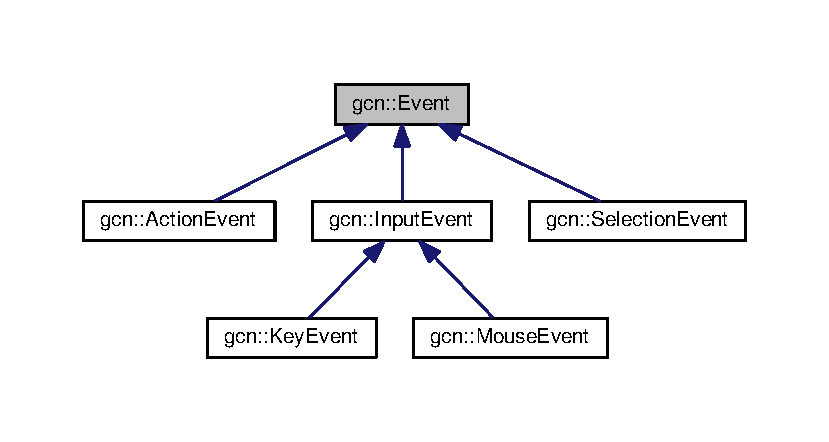
\includegraphics[width=350pt]{classgcn_1_1Event__inherit__graph}
\end{center}
\end{figure}


Collaboration diagram for gcn\+:\+:Event\+:\nopagebreak
\begin{figure}[H]
\begin{center}
\leavevmode
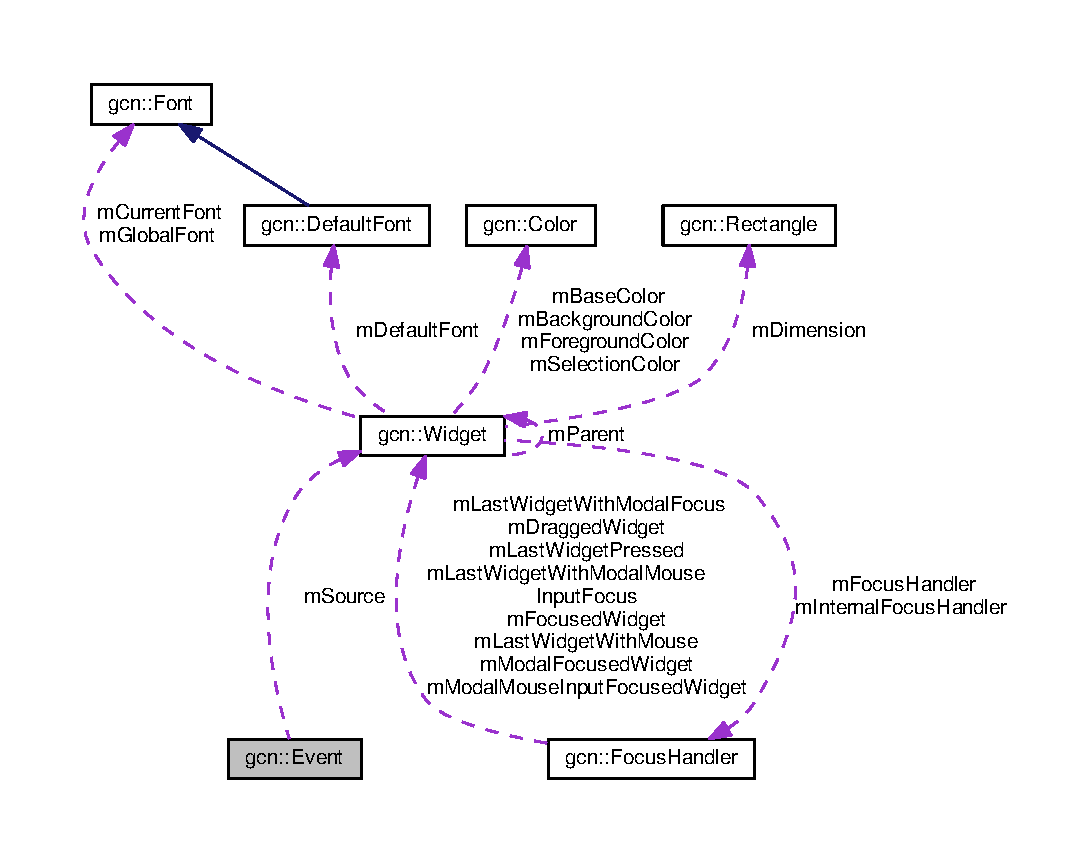
\includegraphics[width=350pt]{classgcn_1_1Event__coll__graph}
\end{center}
\end{figure}
\subsection*{Public Member Functions}
\begin{DoxyCompactItemize}
\item 
\hyperlink{classgcn_1_1Event_ac5db3ce7ebdd2fc5db389b2b14c36098}{Event} (\hyperlink{classgcn_1_1Widget}{Widget} $\ast$source)
\item 
virtual \hyperlink{classgcn_1_1Event_a4bf34f457c9cea588c82986908946303}{$\sim$\+Event} ()
\item 
\hyperlink{classgcn_1_1Widget}{Widget} $\ast$ \hyperlink{classgcn_1_1Event_a21baeb35af32aa708b8438cef922d425}{get\+Source} () const 
\end{DoxyCompactItemize}
\subsection*{Protected Attributes}
\begin{DoxyCompactItemize}
\item 
\hyperlink{classgcn_1_1Widget}{Widget} $\ast$ {\bfseries m\+Source}\hypertarget{classgcn_1_1Event_a062ca3ddb88caba29439543b9b0e95ee}{}\label{classgcn_1_1Event_a062ca3ddb88caba29439543b9b0e95ee}

\item 
unsigned int {\bfseries m\+Type}\hypertarget{classgcn_1_1Event_acffabdf114e116a2dec0fb9ece570b5a}{}\label{classgcn_1_1Event_acffabdf114e116a2dec0fb9ece570b5a}

\end{DoxyCompactItemize}


\subsection{Detailed Description}
Base class for all events.

\begin{DoxyAuthor}{Author}
Olof Naess�n 
\end{DoxyAuthor}
\begin{DoxySince}{Since}
0.\+6.\+0 
\end{DoxySince}


\subsection{Constructor \& Destructor Documentation}
\index{gcn\+::\+Event@{gcn\+::\+Event}!Event@{Event}}
\index{Event@{Event}!gcn\+::\+Event@{gcn\+::\+Event}}
\subsubsection[{\texorpdfstring{Event(\+Widget $\ast$source)}{Event(Widget *source)}}]{\setlength{\rightskip}{0pt plus 5cm}gcn\+::\+Event\+::\+Event (
\begin{DoxyParamCaption}
\item[{{\bf Widget} $\ast$}]{source}
\end{DoxyParamCaption}
)}\hypertarget{classgcn_1_1Event_ac5db3ce7ebdd2fc5db389b2b14c36098}{}\label{classgcn_1_1Event_ac5db3ce7ebdd2fc5db389b2b14c36098}
Constructor.


\begin{DoxyParams}{Parameters}
{\em source} & the source widget of the event. \\
\hline
\end{DoxyParams}
\index{gcn\+::\+Event@{gcn\+::\+Event}!````~Event@{$\sim$\+Event}}
\index{````~Event@{$\sim$\+Event}!gcn\+::\+Event@{gcn\+::\+Event}}
\subsubsection[{\texorpdfstring{$\sim$\+Event()}{~Event()}}]{\setlength{\rightskip}{0pt plus 5cm}gcn\+::\+Event\+::$\sim$\+Event (
\begin{DoxyParamCaption}
{}
\end{DoxyParamCaption}
)\hspace{0.3cm}{\ttfamily [virtual]}}\hypertarget{classgcn_1_1Event_a4bf34f457c9cea588c82986908946303}{}\label{classgcn_1_1Event_a4bf34f457c9cea588c82986908946303}
Destructor. 

\subsection{Member Function Documentation}
\index{gcn\+::\+Event@{gcn\+::\+Event}!get\+Source@{get\+Source}}
\index{get\+Source@{get\+Source}!gcn\+::\+Event@{gcn\+::\+Event}}
\subsubsection[{\texorpdfstring{get\+Source() const }{getSource() const }}]{\setlength{\rightskip}{0pt plus 5cm}{\bf Widget} $\ast$ gcn\+::\+Event\+::get\+Source (
\begin{DoxyParamCaption}
{}
\end{DoxyParamCaption}
) const}\hypertarget{classgcn_1_1Event_a21baeb35af32aa708b8438cef922d425}{}\label{classgcn_1_1Event_a21baeb35af32aa708b8438cef922d425}
Gets the source widget of the event.

\begin{DoxyReturn}{Returns}
the source widget of the event. 
\end{DoxyReturn}


The documentation for this class was generated from the following files\+:\begin{DoxyCompactItemize}
\item 
include/guisan/event.\+hpp\item 
src/event.\+cpp\end{DoxyCompactItemize}

\hypertarget{classgcn_1_1Exception}{}\section{gcn\+:\+:Exception Class Reference}
\label{classgcn_1_1Exception}\index{gcn\+::\+Exception@{gcn\+::\+Exception}}


{\ttfamily \#include $<$exception.\+hpp$>$}

\subsection*{Public Member Functions}
\begin{DoxyCompactItemize}
\item 
\hyperlink{classgcn_1_1Exception_ac6c412a3c4d4f1727b8c847b5dd63bf2}{Exception} ()
\item 
\hyperlink{classgcn_1_1Exception_a4f475350e88e0538f51ec91fb357c729}{Exception} (const std\+::string \&message)
\item 
\hyperlink{classgcn_1_1Exception_ac3bae5d8753050442871681b59b63773}{Exception} (const std\+::string \&message, const std\+::string \&function, const std\+::string \&filename, int line)
\item 
const std\+::string \& \hyperlink{classgcn_1_1Exception_ac409ab0094bd0e9e341f01a532e2fe96}{get\+Function} () const 
\item 
const std\+::string \& \hyperlink{classgcn_1_1Exception_a7c1ca793f383c6dd92eb7fb1694260de}{get\+Message} () const 
\item 
const std\+::string \& \hyperlink{classgcn_1_1Exception_a7918049e3407ace4a59361c1a29b81ac}{get\+Filename} () const 
\item 
int \hyperlink{classgcn_1_1Exception_a93a217b190df8d70405e9feb09c18c00}{get\+Line} () const 
\end{DoxyCompactItemize}
\subsection*{Protected Attributes}
\begin{DoxyCompactItemize}
\item 
std\+::string {\bfseries m\+Function}\hypertarget{classgcn_1_1Exception_ac4cecdef532e30f82d9095789732cfaa}{}\label{classgcn_1_1Exception_ac4cecdef532e30f82d9095789732cfaa}

\item 
std\+::string {\bfseries m\+Message}\hypertarget{classgcn_1_1Exception_a1337ec9291e5587eb2a544212aaa1355}{}\label{classgcn_1_1Exception_a1337ec9291e5587eb2a544212aaa1355}

\item 
std\+::string {\bfseries m\+Filename}\hypertarget{classgcn_1_1Exception_a698a27a1b9d2fba424141d228f5a97a0}{}\label{classgcn_1_1Exception_a698a27a1b9d2fba424141d228f5a97a0}

\item 
int {\bfseries m\+Line}\hypertarget{classgcn_1_1Exception_aaac5868e205d6e89d1546e18ac244daf}{}\label{classgcn_1_1Exception_aaac5868e205d6e89d1546e18ac244daf}

\end{DoxyCompactItemize}


\subsection{Detailed Description}
An exception containing a message, a file and a line number. Guichan will only throw exceptions of this class. You can use this class for your own exceptions. A nifty feature of the excpetion class is that it can tell you from which line and file it was thrown. To make things easier when throwing exceptions there exists a macro for creating exceptions which automatically sets the filename and line number.

E\+X\+A\+M\+P\+LE\+:
\begin{DoxyCode}
\textcolor{keywordflow}{throw} GCN\_EXCEPTION(\textcolor{stringliteral}{"my error message"});
\end{DoxyCode}
 

\subsection{Constructor \& Destructor Documentation}
\index{gcn\+::\+Exception@{gcn\+::\+Exception}!Exception@{Exception}}
\index{Exception@{Exception}!gcn\+::\+Exception@{gcn\+::\+Exception}}
\subsubsection[{\texorpdfstring{Exception()}{Exception()}}]{\setlength{\rightskip}{0pt plus 5cm}gcn\+::\+Exception\+::\+Exception (
\begin{DoxyParamCaption}
{}
\end{DoxyParamCaption}
)}\hypertarget{classgcn_1_1Exception_ac6c412a3c4d4f1727b8c847b5dd63bf2}{}\label{classgcn_1_1Exception_ac6c412a3c4d4f1727b8c847b5dd63bf2}
Constructor. \index{gcn\+::\+Exception@{gcn\+::\+Exception}!Exception@{Exception}}
\index{Exception@{Exception}!gcn\+::\+Exception@{gcn\+::\+Exception}}
\subsubsection[{\texorpdfstring{Exception(const std\+::string \&message)}{Exception(const std::string &message)}}]{\setlength{\rightskip}{0pt plus 5cm}gcn\+::\+Exception\+::\+Exception (
\begin{DoxyParamCaption}
\item[{const std\+::string \&}]{message}
\end{DoxyParamCaption}
)}\hypertarget{classgcn_1_1Exception_a4f475350e88e0538f51ec91fb357c729}{}\label{classgcn_1_1Exception_a4f475350e88e0538f51ec91fb357c729}
Constructor.


\begin{DoxyParams}{Parameters}
{\em message} & the error message. \\
\hline
\end{DoxyParams}
\index{gcn\+::\+Exception@{gcn\+::\+Exception}!Exception@{Exception}}
\index{Exception@{Exception}!gcn\+::\+Exception@{gcn\+::\+Exception}}
\subsubsection[{\texorpdfstring{Exception(const std\+::string \&message, const std\+::string \&function, const std\+::string \&filename, int line)}{Exception(const std::string &message, const std::string &function, const std::string &filename, int line)}}]{\setlength{\rightskip}{0pt plus 5cm}gcn\+::\+Exception\+::\+Exception (
\begin{DoxyParamCaption}
\item[{const std\+::string \&}]{message, }
\item[{const std\+::string \&}]{function, }
\item[{const std\+::string \&}]{filename, }
\item[{int}]{line}
\end{DoxyParamCaption}
)}\hypertarget{classgcn_1_1Exception_ac3bae5d8753050442871681b59b63773}{}\label{classgcn_1_1Exception_ac3bae5d8753050442871681b59b63773}
Constructor.

N\+O\+TE\+: Don\textquotesingle{}t use this constructor. Use the G\+C\+N\+\_\+\+E\+X\+C\+E\+P\+T\+I\+ON macro instead.


\begin{DoxyParams}{Parameters}
{\em message} & the error message. \\
\hline
{\em function} & the function name. \\
\hline
{\em filename} & the name of the file. \\
\hline
{\em line} & the line number. \\
\hline
\end{DoxyParams}


\subsection{Member Function Documentation}
\index{gcn\+::\+Exception@{gcn\+::\+Exception}!get\+Filename@{get\+Filename}}
\index{get\+Filename@{get\+Filename}!gcn\+::\+Exception@{gcn\+::\+Exception}}
\subsubsection[{\texorpdfstring{get\+Filename() const }{getFilename() const }}]{\setlength{\rightskip}{0pt plus 5cm}const std\+::string \& gcn\+::\+Exception\+::get\+Filename (
\begin{DoxyParamCaption}
{}
\end{DoxyParamCaption}
) const}\hypertarget{classgcn_1_1Exception_a7918049e3407ace4a59361c1a29b81ac}{}\label{classgcn_1_1Exception_a7918049e3407ace4a59361c1a29b81ac}
Gets the filename in which the exceptions was thrown.

\begin{DoxyReturn}{Returns}
the filename in which the exception was thrown. 
\end{DoxyReturn}
\index{gcn\+::\+Exception@{gcn\+::\+Exception}!get\+Function@{get\+Function}}
\index{get\+Function@{get\+Function}!gcn\+::\+Exception@{gcn\+::\+Exception}}
\subsubsection[{\texorpdfstring{get\+Function() const }{getFunction() const }}]{\setlength{\rightskip}{0pt plus 5cm}const std\+::string \& gcn\+::\+Exception\+::get\+Function (
\begin{DoxyParamCaption}
{}
\end{DoxyParamCaption}
) const}\hypertarget{classgcn_1_1Exception_ac409ab0094bd0e9e341f01a532e2fe96}{}\label{classgcn_1_1Exception_ac409ab0094bd0e9e341f01a532e2fe96}
Gets the function name in which the exception was thrown.

\begin{DoxyReturn}{Returns}
the function name in which the exception was thrown. 
\end{DoxyReturn}
\index{gcn\+::\+Exception@{gcn\+::\+Exception}!get\+Line@{get\+Line}}
\index{get\+Line@{get\+Line}!gcn\+::\+Exception@{gcn\+::\+Exception}}
\subsubsection[{\texorpdfstring{get\+Line() const }{getLine() const }}]{\setlength{\rightskip}{0pt plus 5cm}int gcn\+::\+Exception\+::get\+Line (
\begin{DoxyParamCaption}
{}
\end{DoxyParamCaption}
) const}\hypertarget{classgcn_1_1Exception_a93a217b190df8d70405e9feb09c18c00}{}\label{classgcn_1_1Exception_a93a217b190df8d70405e9feb09c18c00}
Gets the line number of the line where the exception was thrown.

\begin{DoxyReturn}{Returns}
the line number of the line where the exception was thrown. 
\end{DoxyReturn}
\index{gcn\+::\+Exception@{gcn\+::\+Exception}!get\+Message@{get\+Message}}
\index{get\+Message@{get\+Message}!gcn\+::\+Exception@{gcn\+::\+Exception}}
\subsubsection[{\texorpdfstring{get\+Message() const }{getMessage() const }}]{\setlength{\rightskip}{0pt plus 5cm}const std\+::string \& gcn\+::\+Exception\+::get\+Message (
\begin{DoxyParamCaption}
{}
\end{DoxyParamCaption}
) const}\hypertarget{classgcn_1_1Exception_a7c1ca793f383c6dd92eb7fb1694260de}{}\label{classgcn_1_1Exception_a7c1ca793f383c6dd92eb7fb1694260de}
Gets the error message of the exception.

\begin{DoxyReturn}{Returns}
the error message. 
\end{DoxyReturn}


The documentation for this class was generated from the following files\+:\begin{DoxyCompactItemize}
\item 
include/guisan/exception.\+hpp\item 
src/exception.\+cpp\end{DoxyCompactItemize}

\hypertarget{classFFCharacterChooser}{}\section{F\+F\+Character\+Chooser Class Reference}
\label{classFFCharacterChooser}\index{F\+F\+Character\+Chooser@{F\+F\+Character\+Chooser}}


Inheritance diagram for F\+F\+Character\+Chooser\+:\nopagebreak
\begin{figure}[H]
\begin{center}
\leavevmode
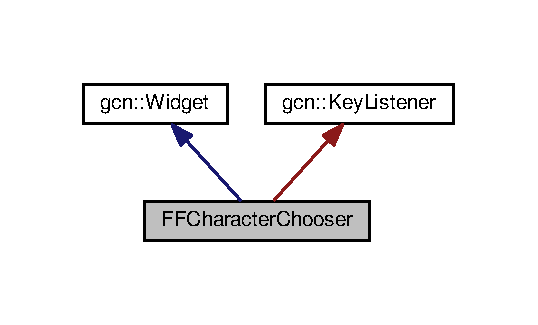
\includegraphics[width=258pt]{classFFCharacterChooser__inherit__graph}
\end{center}
\end{figure}


Collaboration diagram for F\+F\+Character\+Chooser\+:\nopagebreak
\begin{figure}[H]
\begin{center}
\leavevmode
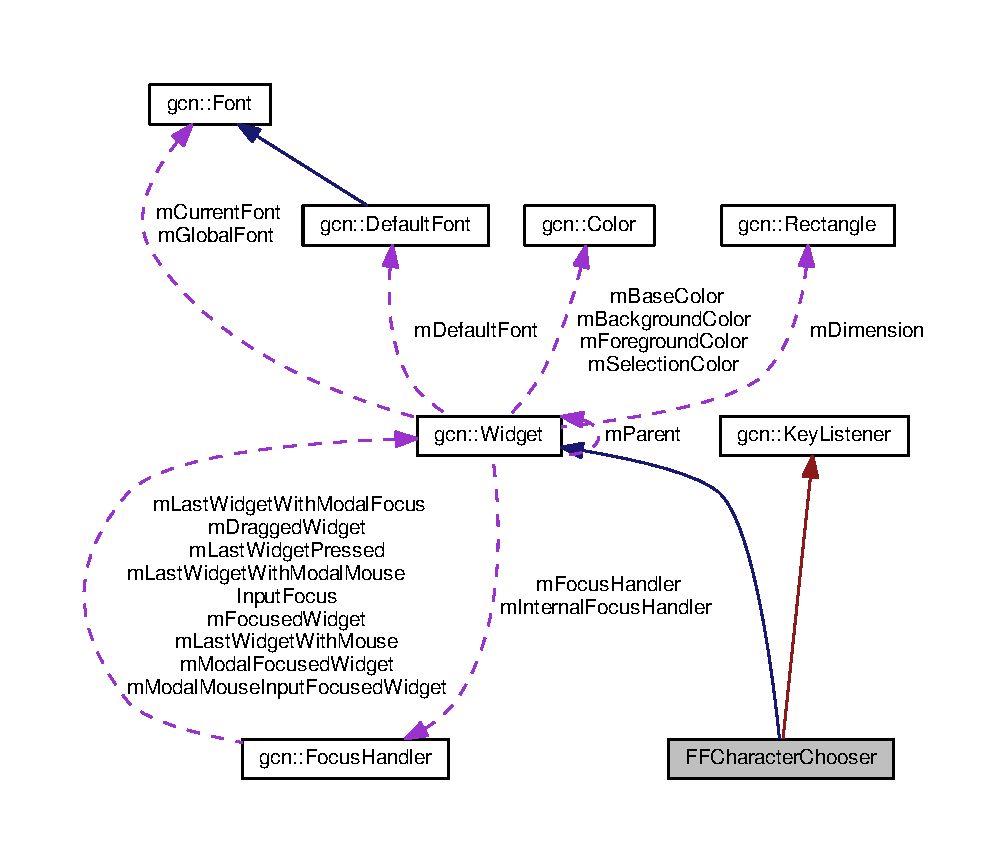
\includegraphics[width=350pt]{classFFCharacterChooser__coll__graph}
\end{center}
\end{figure}
\subsection*{Public Member Functions}
\begin{DoxyCompactItemize}
\item 
void \hyperlink{classFFCharacterChooser_a5201030dd120d58eb0470269649a3541}{draw} (\hyperlink{classgcn_1_1Graphics}{gcn\+::\+Graphics} $\ast$graphics)
\item 
int {\bfseries get\+Selected} ()\hypertarget{classFFCharacterChooser_a45a2b60a3a6e36b5f5ab8c482995f4ca}{}\label{classFFCharacterChooser_a45a2b60a3a6e36b5f5ab8c482995f4ca}

\item 
void {\bfseries set\+Selected} (int selected)\hypertarget{classFFCharacterChooser_af195b46f2389b2a72d287344316fa795}{}\label{classFFCharacterChooser_af195b46f2389b2a72d287344316fa795}

\item 
void {\bfseries set\+Distance} (int distance)\hypertarget{classFFCharacterChooser_a9f4cb567c877350287a85f8688f86e32}{}\label{classFFCharacterChooser_a9f4cb567c877350287a85f8688f86e32}

\item 
void \hyperlink{classFFCharacterChooser_a34d12f0a5f7588ee8dc36da24a75c7df}{key\+Pressed} (\hyperlink{classgcn_1_1KeyEvent}{gcn\+::\+Key\+Event} \&key\+Event)
\end{DoxyCompactItemize}
\subsection*{Additional Inherited Members}


\subsection{Member Function Documentation}
\index{F\+F\+Character\+Chooser@{F\+F\+Character\+Chooser}!draw@{draw}}
\index{draw@{draw}!F\+F\+Character\+Chooser@{F\+F\+Character\+Chooser}}
\subsubsection[{\texorpdfstring{draw(gcn\+::\+Graphics $\ast$graphics)}{draw(gcn::Graphics *graphics)}}]{\setlength{\rightskip}{0pt plus 5cm}void F\+F\+Character\+Chooser\+::draw (
\begin{DoxyParamCaption}
\item[{{\bf gcn\+::\+Graphics} $\ast$}]{graphics}
\end{DoxyParamCaption}
)\hspace{0.3cm}{\ttfamily [virtual]}}\hypertarget{classFFCharacterChooser_a5201030dd120d58eb0470269649a3541}{}\label{classFFCharacterChooser_a5201030dd120d58eb0470269649a3541}
Draws the widget. It is called by the parent widget when it is time for the widget to draw itself. The graphics object is set up so that all drawing is relative to the widget, i.\+e coordinate (0,0) is the top-\/left corner of the widget. It is not possible to draw outside of a widgets dimension.


\begin{DoxyParams}{Parameters}
{\em graphics} & a Graphics object to draw with. \\
\hline
\end{DoxyParams}


Implements \hyperlink{classgcn_1_1Widget_acc595221d6a2d1afe1043c16dc37d212}{gcn\+::\+Widget}.

\index{F\+F\+Character\+Chooser@{F\+F\+Character\+Chooser}!key\+Pressed@{key\+Pressed}}
\index{key\+Pressed@{key\+Pressed}!F\+F\+Character\+Chooser@{F\+F\+Character\+Chooser}}
\subsubsection[{\texorpdfstring{key\+Pressed(gcn\+::\+Key\+Event \&key\+Event)}{keyPressed(gcn::KeyEvent &keyEvent)}}]{\setlength{\rightskip}{0pt plus 5cm}void F\+F\+Character\+Chooser\+::key\+Pressed (
\begin{DoxyParamCaption}
\item[{{\bf gcn\+::\+Key\+Event} \&}]{key\+Event}
\end{DoxyParamCaption}
)\hspace{0.3cm}{\ttfamily [virtual]}}\hypertarget{classFFCharacterChooser_a34d12f0a5f7588ee8dc36da24a75c7df}{}\label{classFFCharacterChooser_a34d12f0a5f7588ee8dc36da24a75c7df}
Called if a key is pressed when the widget has keyboard focus. If a key is held down the widget will generate multiple key presses.


\begin{DoxyParams}{Parameters}
{\em key\+Event} & discribes the event. \\
\hline
\end{DoxyParams}


Reimplemented from \hyperlink{classgcn_1_1KeyListener_ada6c0d038340d6ee674702268b2d2c67}{gcn\+::\+Key\+Listener}.



The documentation for this class was generated from the following files\+:\begin{DoxyCompactItemize}
\item 
demo/include/ffcharacterchooser.\+hpp\item 
demo/src/ffcharacterchooser.\+cpp\end{DoxyCompactItemize}

\hypertarget{classFFContainer}{}\section{F\+F\+Container Class Reference}
\label{classFFContainer}\index{F\+F\+Container@{F\+F\+Container}}


Inheritance diagram for F\+F\+Container\+:\nopagebreak
\begin{figure}[H]
\begin{center}
\leavevmode
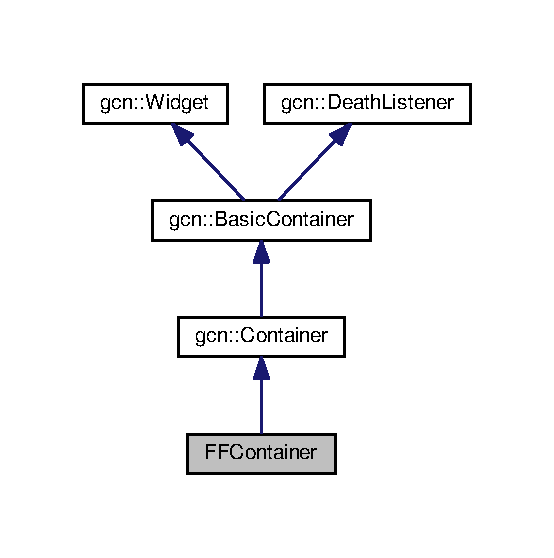
\includegraphics[width=266pt]{classFFContainer__inherit__graph}
\end{center}
\end{figure}


Collaboration diagram for F\+F\+Container\+:\nopagebreak
\begin{figure}[H]
\begin{center}
\leavevmode
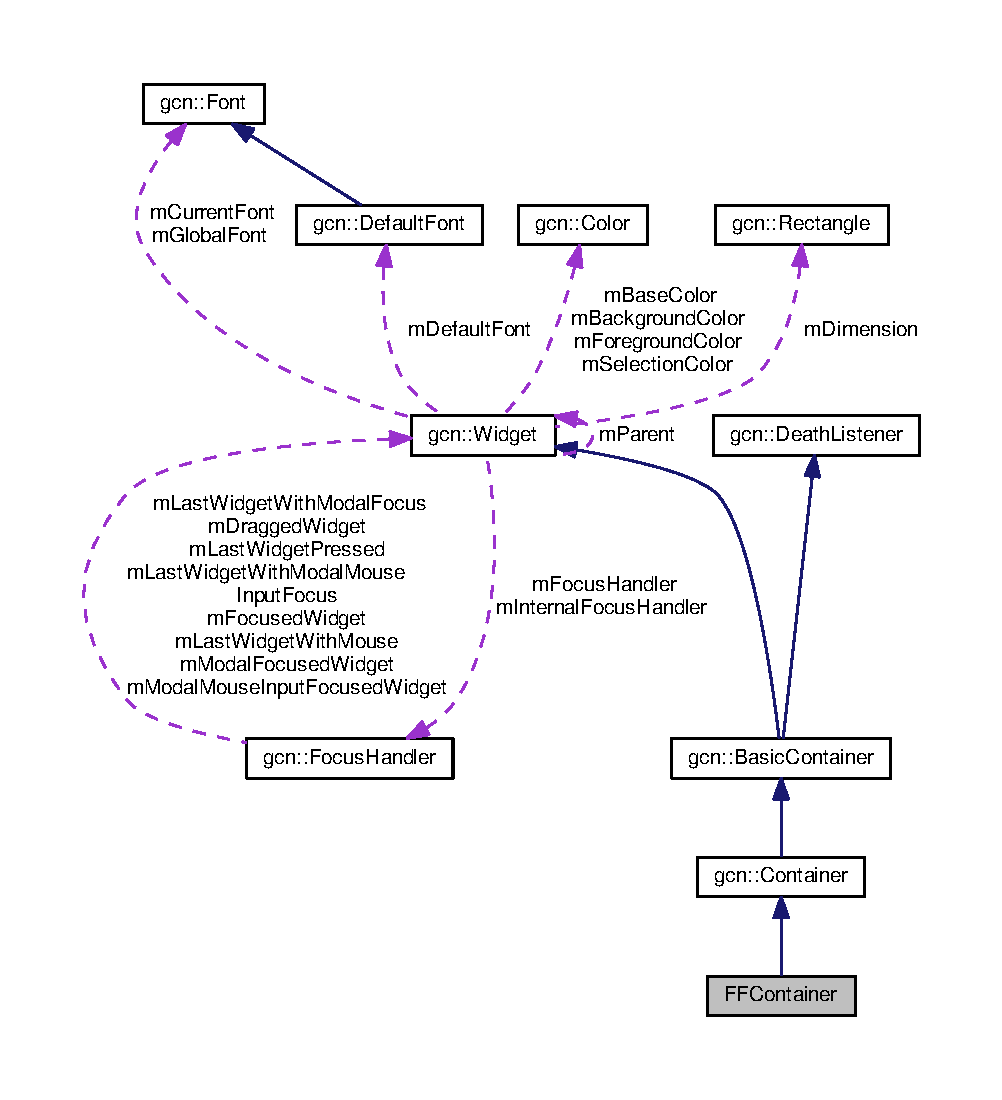
\includegraphics[width=350pt]{classFFContainer__coll__graph}
\end{center}
\end{figure}
\subsection*{Public Member Functions}
\begin{DoxyCompactItemize}
\item 
void \hyperlink{classFFContainer_a5d53541089f719665bfc2d689dab89c6}{logic} ()
\item 
void \hyperlink{classFFContainer_a42352820e4ed070f831a84a8b51451c6}{draw} (\hyperlink{classgcn_1_1Graphics}{gcn\+::\+Graphics} $\ast$graphics)
\item 
void {\bfseries set\+Visible} (bool visible)\hypertarget{classFFContainer_a7b79e941fd38a871b2b893858b786ce1}{}\label{classFFContainer_a7b79e941fd38a871b2b893858b786ce1}

\item 
void {\bfseries set\+Width} (int width)\hypertarget{classFFContainer_a4f1f5ba45a48ecfba79e7ec88ee6b010}{}\label{classFFContainer_a4f1f5ba45a48ecfba79e7ec88ee6b010}

\item 
void {\bfseries set\+Height} (int width)\hypertarget{classFFContainer_aa91986bab12d8ea8598d8b712959f40f}{}\label{classFFContainer_aa91986bab12d8ea8598d8b712959f40f}

\item 
void {\bfseries set\+Dimension} (const \hyperlink{classgcn_1_1Rectangle}{gcn\+::\+Rectangle} \&dimension)\hypertarget{classFFContainer_a271182e93c5317594d5e71e4db3074ae}{}\label{classFFContainer_a271182e93c5317594d5e71e4db3074ae}

\item 
void {\bfseries slide\+Content\+To} (int y)\hypertarget{classFFContainer_a551953811ba44c76aad11733897f7960}{}\label{classFFContainer_a551953811ba44c76aad11733897f7960}

\item 
\hyperlink{classgcn_1_1Rectangle}{gcn\+::\+Rectangle} \hyperlink{classFFContainer_af509106f3e9c8d69e821d864abfa1f7d}{get\+Children\+Area} ()
\end{DoxyCompactItemize}
\subsection*{Additional Inherited Members}


\subsection{Member Function Documentation}
\index{F\+F\+Container@{F\+F\+Container}!draw@{draw}}
\index{draw@{draw}!F\+F\+Container@{F\+F\+Container}}
\subsubsection[{\texorpdfstring{draw(gcn\+::\+Graphics $\ast$graphics)}{draw(gcn::Graphics *graphics)}}]{\setlength{\rightskip}{0pt plus 5cm}void F\+F\+Container\+::draw (
\begin{DoxyParamCaption}
\item[{{\bf gcn\+::\+Graphics} $\ast$}]{graphics}
\end{DoxyParamCaption}
)\hspace{0.3cm}{\ttfamily [virtual]}}\hypertarget{classFFContainer_a42352820e4ed070f831a84a8b51451c6}{}\label{classFFContainer_a42352820e4ed070f831a84a8b51451c6}
Draws the widget. It is called by the parent widget when it is time for the widget to draw itself. The graphics object is set up so that all drawing is relative to the widget, i.\+e coordinate (0,0) is the top-\/left corner of the widget. It is not possible to draw outside of a widgets dimension.


\begin{DoxyParams}{Parameters}
{\em graphics} & a Graphics object to draw with. \\
\hline
\end{DoxyParams}


Reimplemented from \hyperlink{classgcn_1_1Container_a0bc3386f5564165fcb13e9d389a96432}{gcn\+::\+Container}.

\index{F\+F\+Container@{F\+F\+Container}!get\+Children\+Area@{get\+Children\+Area}}
\index{get\+Children\+Area@{get\+Children\+Area}!F\+F\+Container@{F\+F\+Container}}
\subsubsection[{\texorpdfstring{get\+Children\+Area()}{getChildrenArea()}}]{\setlength{\rightskip}{0pt plus 5cm}{\bf gcn\+::\+Rectangle} F\+F\+Container\+::get\+Children\+Area (
\begin{DoxyParamCaption}
{}
\end{DoxyParamCaption}
)\hspace{0.3cm}{\ttfamily [virtual]}}\hypertarget{classFFContainer_af509106f3e9c8d69e821d864abfa1f7d}{}\label{classFFContainer_af509106f3e9c8d69e821d864abfa1f7d}
Gets the subarea of the widget that the children occupy.

\begin{DoxyReturn}{Returns}
the subarea as a Rectangle. 
\end{DoxyReturn}


Reimplemented from \hyperlink{classgcn_1_1BasicContainer_a8ed853146d726cb3bc5d109ad52203d6}{gcn\+::\+Basic\+Container}.

\index{F\+F\+Container@{F\+F\+Container}!logic@{logic}}
\index{logic@{logic}!F\+F\+Container@{F\+F\+Container}}
\subsubsection[{\texorpdfstring{logic()}{logic()}}]{\setlength{\rightskip}{0pt plus 5cm}void F\+F\+Container\+::logic (
\begin{DoxyParamCaption}
{}
\end{DoxyParamCaption}
)\hspace{0.3cm}{\ttfamily [virtual]}}\hypertarget{classFFContainer_a5d53541089f719665bfc2d689dab89c6}{}\label{classFFContainer_a5d53541089f719665bfc2d689dab89c6}
Called for all widgets in the gui each time Gui\+::logic is called. You can do logic stuff here like playing an animation.

\begin{DoxySeeAlso}{See also}
Gui 
\end{DoxySeeAlso}


Reimplemented from \hyperlink{classgcn_1_1BasicContainer_a65972968364c62bf244985b2900eaf25}{gcn\+::\+Basic\+Container}.



The documentation for this class was generated from the following files\+:\begin{DoxyCompactItemize}
\item 
demo/include/ffcontainer.\+hpp\item 
demo/src/ffcontainer.\+cpp\end{DoxyCompactItemize}

\hypertarget{classFFDemo}{}\section{F\+F\+Demo Class Reference}
\label{classFFDemo}\index{F\+F\+Demo@{F\+F\+Demo}}


Inheritance diagram for F\+F\+Demo\+:\nopagebreak
\begin{figure}[H]
\begin{center}
\leavevmode
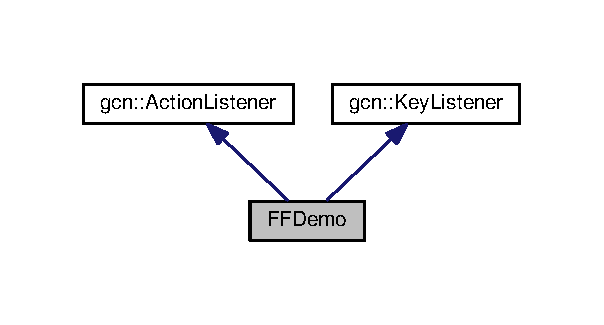
\includegraphics[width=290pt]{classFFDemo__inherit__graph}
\end{center}
\end{figure}


Collaboration diagram for F\+F\+Demo\+:\nopagebreak
\begin{figure}[H]
\begin{center}
\leavevmode
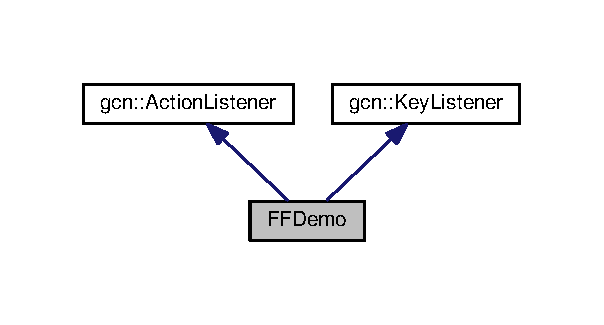
\includegraphics[width=290pt]{classFFDemo__coll__graph}
\end{center}
\end{figure}
\subsection*{Public Member Functions}
\begin{DoxyCompactItemize}
\item 
void {\bfseries run} ()\hypertarget{classFFDemo_ae138571c8d71404ca992bb2d7b9ae658}{}\label{classFFDemo_ae138571c8d71404ca992bb2d7b9ae658}

\item 
void \hyperlink{classFFDemo_ab7c02fe745edd2e4de4a9fd17b30abc2}{action} (const \hyperlink{classgcn_1_1ActionEvent}{gcn\+::\+Action\+Event} \&action\+Event)
\item 
void \hyperlink{classFFDemo_a0307231911726663da3e9f641601ada5}{key\+Pressed} (\hyperlink{classgcn_1_1KeyEvent}{gcn\+::\+Key\+Event} \&key\+Event)
\end{DoxyCompactItemize}
\subsection*{Additional Inherited Members}


\subsection{Member Function Documentation}
\index{F\+F\+Demo@{F\+F\+Demo}!action@{action}}
\index{action@{action}!F\+F\+Demo@{F\+F\+Demo}}
\subsubsection[{\texorpdfstring{action(const gcn\+::\+Action\+Event \&action\+Event)}{action(const gcn::ActionEvent &actionEvent)}}]{\setlength{\rightskip}{0pt plus 5cm}void F\+F\+Demo\+::action (
\begin{DoxyParamCaption}
\item[{const {\bf gcn\+::\+Action\+Event} \&}]{action\+Event}
\end{DoxyParamCaption}
)\hspace{0.3cm}{\ttfamily [virtual]}}\hypertarget{classFFDemo_ab7c02fe745edd2e4de4a9fd17b30abc2}{}\label{classFFDemo_ab7c02fe745edd2e4de4a9fd17b30abc2}
Called when an action is recieved from a Widget. It is used to be able to recieve a notification that an action has occured.


\begin{DoxyParams}{Parameters}
{\em action\+Event} & the event of the action. \\
\hline
\end{DoxyParams}
\begin{DoxySince}{Since}
0.\+6.\+0 
\end{DoxySince}


Implements \hyperlink{classgcn_1_1ActionListener_ae883112ab054a8589b5d82c47763a31d}{gcn\+::\+Action\+Listener}.

\index{F\+F\+Demo@{F\+F\+Demo}!key\+Pressed@{key\+Pressed}}
\index{key\+Pressed@{key\+Pressed}!F\+F\+Demo@{F\+F\+Demo}}
\subsubsection[{\texorpdfstring{key\+Pressed(gcn\+::\+Key\+Event \&key\+Event)}{keyPressed(gcn::KeyEvent &keyEvent)}}]{\setlength{\rightskip}{0pt plus 5cm}void F\+F\+Demo\+::key\+Pressed (
\begin{DoxyParamCaption}
\item[{{\bf gcn\+::\+Key\+Event} \&}]{key\+Event}
\end{DoxyParamCaption}
)\hspace{0.3cm}{\ttfamily [virtual]}}\hypertarget{classFFDemo_a0307231911726663da3e9f641601ada5}{}\label{classFFDemo_a0307231911726663da3e9f641601ada5}
Called if a key is pressed when the widget has keyboard focus. If a key is held down the widget will generate multiple key presses.


\begin{DoxyParams}{Parameters}
{\em key\+Event} & discribes the event. \\
\hline
\end{DoxyParams}


Reimplemented from \hyperlink{classgcn_1_1KeyListener_ada6c0d038340d6ee674702268b2d2c67}{gcn\+::\+Key\+Listener}.



The documentation for this class was generated from the following files\+:\begin{DoxyCompactItemize}
\item 
demo/include/ffdemo.\+hpp\item 
demo/src/ffdemo.\+cpp\end{DoxyCompactItemize}

\hypertarget{classFFListBox}{}\section{F\+F\+List\+Box Class Reference}
\label{classFFListBox}\index{F\+F\+List\+Box@{F\+F\+List\+Box}}


Inheritance diagram for F\+F\+List\+Box\+:\nopagebreak
\begin{figure}[H]
\begin{center}
\leavevmode
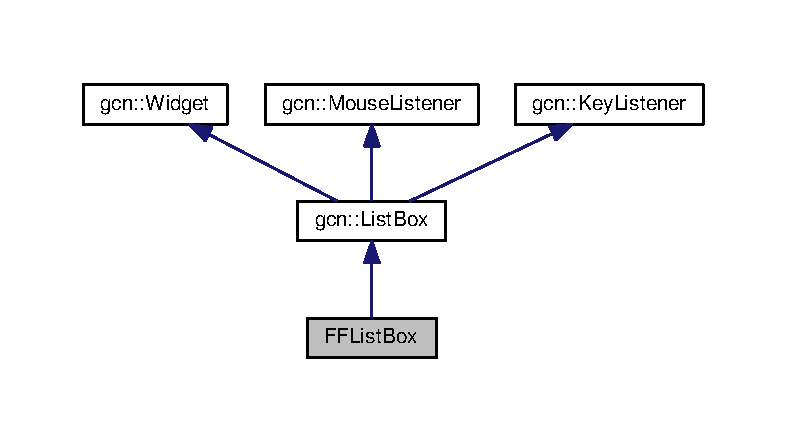
\includegraphics[width=350pt]{classFFListBox__inherit__graph}
\end{center}
\end{figure}


Collaboration diagram for F\+F\+List\+Box\+:\nopagebreak
\begin{figure}[H]
\begin{center}
\leavevmode
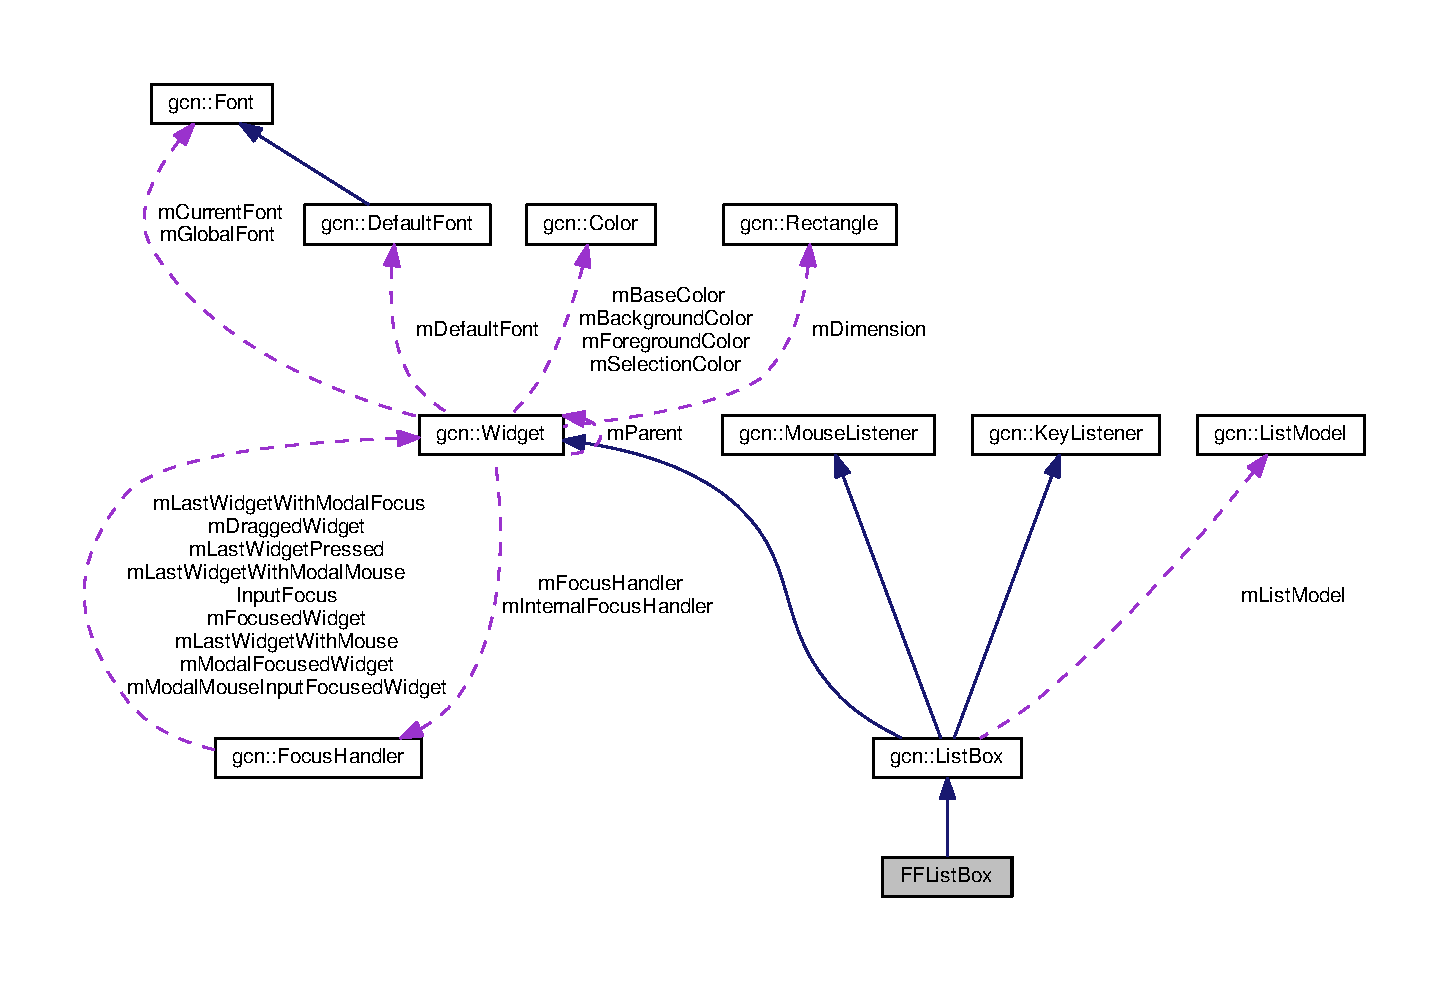
\includegraphics[width=350pt]{classFFListBox__coll__graph}
\end{center}
\end{figure}
\subsection*{Public Member Functions}
\begin{DoxyCompactItemize}
\item 
void \hyperlink{classFFListBox_a37cb82f6ca370d2065107079454b086d}{draw} (\hyperlink{classgcn_1_1Graphics}{gcn\+::\+Graphics} $\ast$graphics)
\item 
void {\bfseries set\+Selected} (int i)\hypertarget{classFFListBox_ac1ed7a25db5b010b15918366756be2db}{}\label{classFFListBox_ac1ed7a25db5b010b15918366756be2db}

\end{DoxyCompactItemize}
\subsection*{Additional Inherited Members}


\subsection{Member Function Documentation}
\index{F\+F\+List\+Box@{F\+F\+List\+Box}!draw@{draw}}
\index{draw@{draw}!F\+F\+List\+Box@{F\+F\+List\+Box}}
\subsubsection[{\texorpdfstring{draw(gcn\+::\+Graphics $\ast$graphics)}{draw(gcn::Graphics *graphics)}}]{\setlength{\rightskip}{0pt plus 5cm}void F\+F\+List\+Box\+::draw (
\begin{DoxyParamCaption}
\item[{{\bf gcn\+::\+Graphics} $\ast$}]{graphics}
\end{DoxyParamCaption}
)\hspace{0.3cm}{\ttfamily [virtual]}}\hypertarget{classFFListBox_a37cb82f6ca370d2065107079454b086d}{}\label{classFFListBox_a37cb82f6ca370d2065107079454b086d}
Draws the widget. It is called by the parent widget when it is time for the widget to draw itself. The graphics object is set up so that all drawing is relative to the widget, i.\+e coordinate (0,0) is the top-\/left corner of the widget. It is not possible to draw outside of a widgets dimension.


\begin{DoxyParams}{Parameters}
{\em graphics} & a Graphics object to draw with. \\
\hline
\end{DoxyParams}
\begin{DoxyRefDesc}{Todo}
\item[\hyperlink{todo__todo000001}{Todo}]Check cliprects so we do not have to iterate over elements in the list model \end{DoxyRefDesc}


Reimplemented from \hyperlink{classgcn_1_1ListBox_a6c12d3659318a214896f56ab704a78b6}{gcn\+::\+List\+Box}.



The documentation for this class was generated from the following files\+:\begin{DoxyCompactItemize}
\item 
demo/include/fflistbox.\+hpp\item 
demo/src/fflistbox.\+cpp\end{DoxyCompactItemize}

\hypertarget{classFFScrollArea}{}\section{F\+F\+Scroll\+Area Class Reference}
\label{classFFScrollArea}\index{F\+F\+Scroll\+Area@{F\+F\+Scroll\+Area}}


Inheritance diagram for F\+F\+Scroll\+Area\+:\nopagebreak
\begin{figure}[H]
\begin{center}
\leavevmode
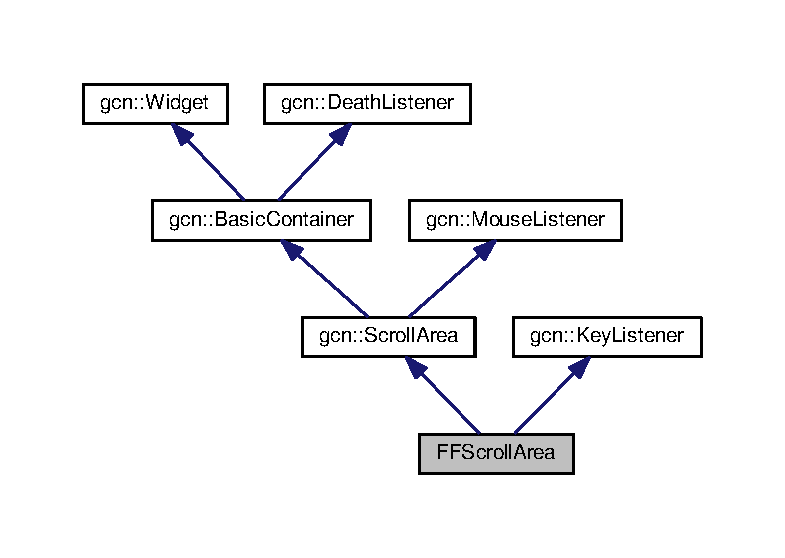
\includegraphics[width=350pt]{classFFScrollArea__inherit__graph}
\end{center}
\end{figure}


Collaboration diagram for F\+F\+Scroll\+Area\+:\nopagebreak
\begin{figure}[H]
\begin{center}
\leavevmode
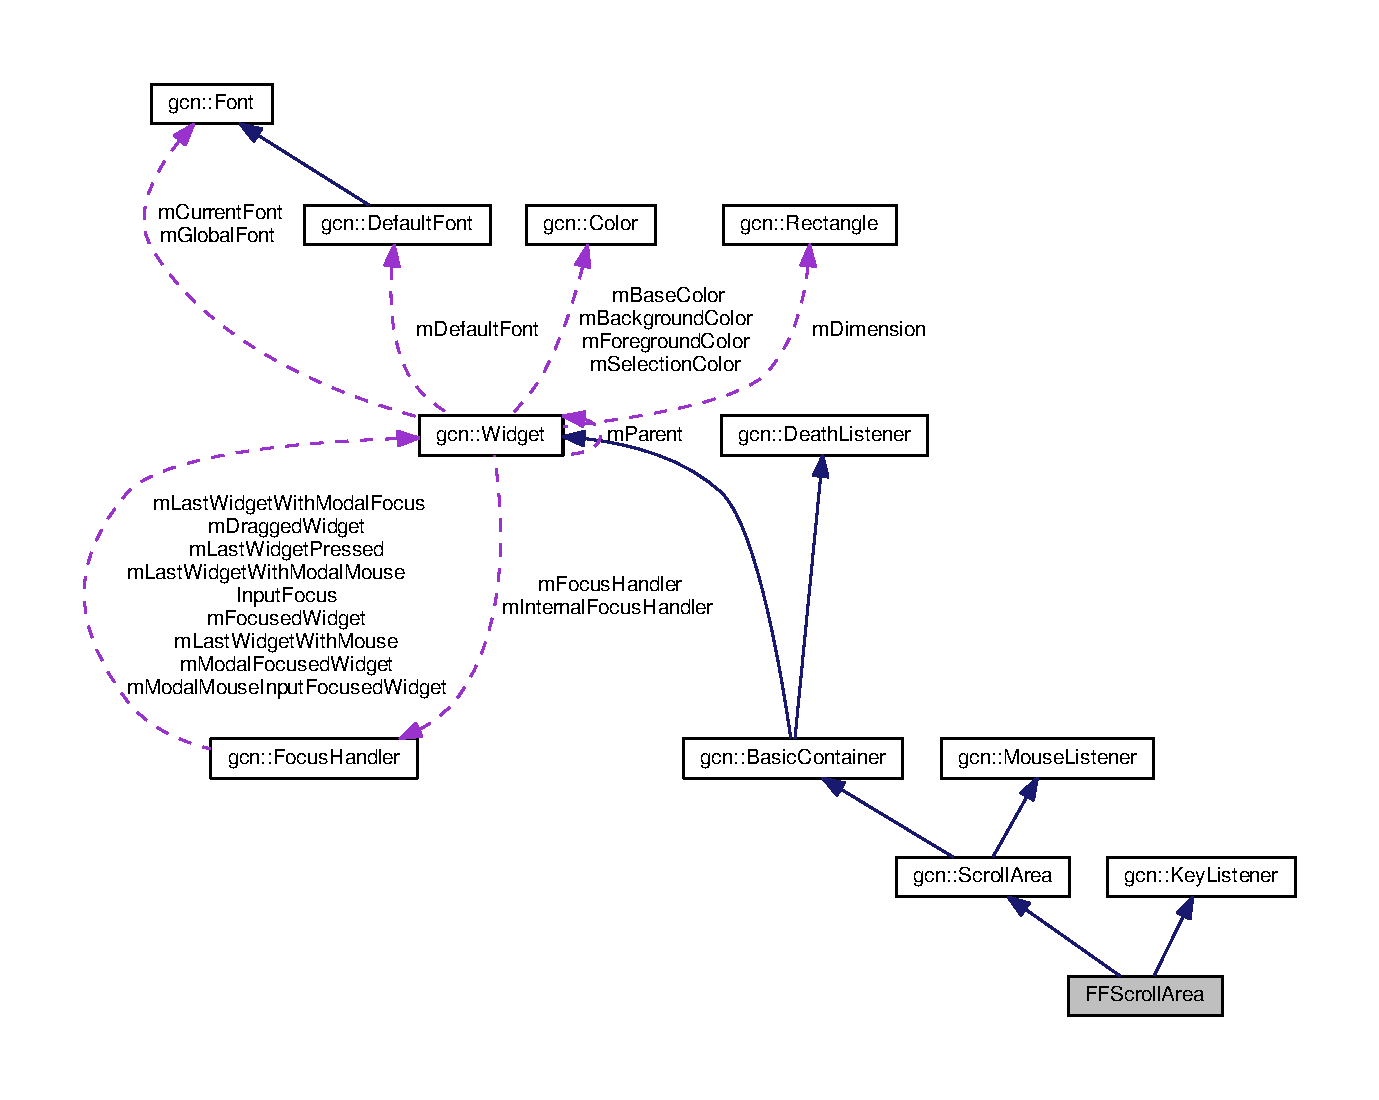
\includegraphics[width=350pt]{classFFScrollArea__coll__graph}
\end{center}
\end{figure}
\subsection*{Public Member Functions}
\begin{DoxyCompactItemize}
\item 
void \hyperlink{classFFScrollArea_a79b4d005445cb2909e355ad75c19021b}{draw} (\hyperlink{classgcn_1_1Graphics}{gcn\+::\+Graphics} $\ast$graphics)
\item 
void \hyperlink{classFFScrollArea_ae66ca9f4f9e738fd30af79b2517ca95f}{key\+Pressed} (\hyperlink{classgcn_1_1KeyEvent}{gcn\+::\+Key\+Event} \&key\+Event)
\end{DoxyCompactItemize}
\subsection*{Additional Inherited Members}


\subsection{Member Function Documentation}
\index{F\+F\+Scroll\+Area@{F\+F\+Scroll\+Area}!draw@{draw}}
\index{draw@{draw}!F\+F\+Scroll\+Area@{F\+F\+Scroll\+Area}}
\subsubsection[{\texorpdfstring{draw(gcn\+::\+Graphics $\ast$graphics)}{draw(gcn::Graphics *graphics)}}]{\setlength{\rightskip}{0pt plus 5cm}void F\+F\+Scroll\+Area\+::draw (
\begin{DoxyParamCaption}
\item[{{\bf gcn\+::\+Graphics} $\ast$}]{graphics}
\end{DoxyParamCaption}
)\hspace{0.3cm}{\ttfamily [virtual]}}\hypertarget{classFFScrollArea_a79b4d005445cb2909e355ad75c19021b}{}\label{classFFScrollArea_a79b4d005445cb2909e355ad75c19021b}
Draws the widget. It is called by the parent widget when it is time for the widget to draw itself. The graphics object is set up so that all drawing is relative to the widget, i.\+e coordinate (0,0) is the top-\/left corner of the widget. It is not possible to draw outside of a widgets dimension.


\begin{DoxyParams}{Parameters}
{\em graphics} & a Graphics object to draw with. \\
\hline
\end{DoxyParams}


Reimplemented from \hyperlink{classgcn_1_1ScrollArea_a2bab40dcb6d851aec51104efb934744c}{gcn\+::\+Scroll\+Area}.

\index{F\+F\+Scroll\+Area@{F\+F\+Scroll\+Area}!key\+Pressed@{key\+Pressed}}
\index{key\+Pressed@{key\+Pressed}!F\+F\+Scroll\+Area@{F\+F\+Scroll\+Area}}
\subsubsection[{\texorpdfstring{key\+Pressed(gcn\+::\+Key\+Event \&key\+Event)}{keyPressed(gcn::KeyEvent &keyEvent)}}]{\setlength{\rightskip}{0pt plus 5cm}void F\+F\+Scroll\+Area\+::key\+Pressed (
\begin{DoxyParamCaption}
\item[{{\bf gcn\+::\+Key\+Event} \&}]{key\+Event}
\end{DoxyParamCaption}
)\hspace{0.3cm}{\ttfamily [virtual]}}\hypertarget{classFFScrollArea_ae66ca9f4f9e738fd30af79b2517ca95f}{}\label{classFFScrollArea_ae66ca9f4f9e738fd30af79b2517ca95f}
Called if a key is pressed when the widget has keyboard focus. If a key is held down the widget will generate multiple key presses.


\begin{DoxyParams}{Parameters}
{\em key\+Event} & discribes the event. \\
\hline
\end{DoxyParams}


Reimplemented from \hyperlink{classgcn_1_1KeyListener_ada6c0d038340d6ee674702268b2d2c67}{gcn\+::\+Key\+Listener}.



The documentation for this class was generated from the following files\+:\begin{DoxyCompactItemize}
\item 
demo/include/ffscrollarea.\+hpp\item 
demo/src/ffscrollarea.\+cpp\end{DoxyCompactItemize}

\hypertarget{classgcn_1_1FocusHandler}{}\section{gcn\+:\+:Focus\+Handler Class Reference}
\label{classgcn_1_1FocusHandler}\index{gcn\+::\+Focus\+Handler@{gcn\+::\+Focus\+Handler}}


{\ttfamily \#include $<$focushandler.\+hpp$>$}



Collaboration diagram for gcn\+:\+:Focus\+Handler\+:\nopagebreak
\begin{figure}[H]
\begin{center}
\leavevmode
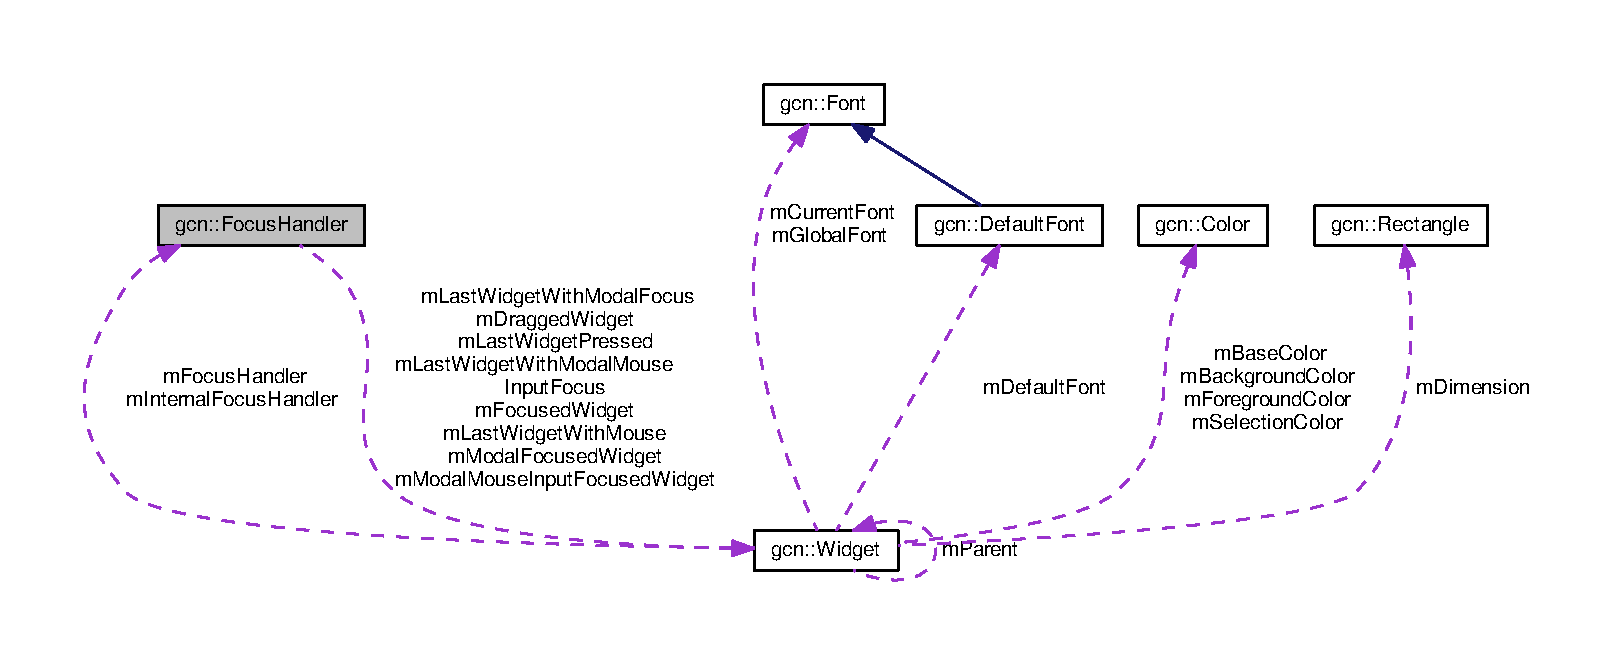
\includegraphics[width=350pt]{classgcn_1_1FocusHandler__coll__graph}
\end{center}
\end{figure}
\subsection*{Public Member Functions}
\begin{DoxyCompactItemize}
\item 
\hyperlink{classgcn_1_1FocusHandler_a41eeb97436bdf9931d4d3207f451f749}{Focus\+Handler} ()
\item 
virtual \hyperlink{classgcn_1_1FocusHandler_a968758e15ea32627a5d464b749772e3c}{$\sim$\+Focus\+Handler} ()
\item 
virtual void \hyperlink{classgcn_1_1FocusHandler_a34338442a14a395d15b43aabcc6f8139}{request\+Focus} (\hyperlink{classgcn_1_1Widget}{Widget} $\ast$widget)
\item 
virtual void \hyperlink{classgcn_1_1FocusHandler_a2ae2d6b3d2cf09f2ebec9300349832e2}{request\+Modal\+Focus} (\hyperlink{classgcn_1_1Widget}{Widget} $\ast$widget)
\item 
virtual void \hyperlink{classgcn_1_1FocusHandler_a3836b151410948ab12cdf83fd106cd66}{release\+Modal\+Focus} (\hyperlink{classgcn_1_1Widget}{Widget} $\ast$widget)
\item 
virtual void \hyperlink{classgcn_1_1FocusHandler_a3a38e6449b095e5a1eb0dc435998a0fc}{request\+Modal\+Mouse\+Input\+Focus} (\hyperlink{classgcn_1_1Widget}{Widget} $\ast$widget)
\item 
virtual void \hyperlink{classgcn_1_1FocusHandler_a264a639d3ee8fd1bce3da98ab4e9b801}{release\+Modal\+Mouse\+Input\+Focus} (\hyperlink{classgcn_1_1Widget}{Widget} $\ast$widget)
\item 
virtual \hyperlink{classgcn_1_1Widget}{Widget} $\ast$ \hyperlink{classgcn_1_1FocusHandler_abf39461c7677d6dec8df55eab468916f}{get\+Focused} () const 
\item 
virtual \hyperlink{classgcn_1_1Widget}{Widget} $\ast$ \hyperlink{classgcn_1_1FocusHandler_a40596b967f719cef214a31396a8fd28d}{get\+Modal\+Focused} () const 
\item 
virtual \hyperlink{classgcn_1_1Widget}{Widget} $\ast$ \hyperlink{classgcn_1_1FocusHandler_af0aa61ebec5566ad1a5c46a90606f053}{get\+Modal\+Mouse\+Input\+Focused} () const 
\item 
virtual void \hyperlink{classgcn_1_1FocusHandler_a4d6014146d5066a00ea1e7cdeebf63ec}{focus\+Next} ()
\item 
virtual void \hyperlink{classgcn_1_1FocusHandler_aa4551f5bfaa832c7d25d91cc94ba95fc}{focus\+Previous} ()
\item 
virtual bool \hyperlink{classgcn_1_1FocusHandler_ac7fccb6de0fb3ec53ac9a8c60aa03f3a}{is\+Focused} (const \hyperlink{classgcn_1_1Widget}{Widget} $\ast$widget) const 
\item 
virtual void \hyperlink{classgcn_1_1FocusHandler_a8ae5c1b60bf81d2903a34b5dc207e5ee}{add} (\hyperlink{classgcn_1_1Widget}{Widget} $\ast$widget)
\item 
virtual void \hyperlink{classgcn_1_1FocusHandler_afa5123828555a1a98fe85e4afb1ae816}{remove} (\hyperlink{classgcn_1_1Widget}{Widget} $\ast$widget)
\item 
virtual void \hyperlink{classgcn_1_1FocusHandler_a35de8a2fb79bc79cfd232a70755ee936}{focus\+None} ()
\item 
virtual void \hyperlink{classgcn_1_1FocusHandler_a4a7ccd8c411cb8a36f6e8d0f27e2cdf7}{tab\+Next} ()
\item 
virtual void \hyperlink{classgcn_1_1FocusHandler_aa1e04e171d46af448f18c0217075b1cc}{tab\+Previous} ()
\item 
virtual \hyperlink{classgcn_1_1Widget}{Widget} $\ast$ \hyperlink{classgcn_1_1FocusHandler_ad1bc219a7d9d6a564b0f986e31b773d6}{get\+Dragged\+Widget} ()
\item 
virtual void \hyperlink{classgcn_1_1FocusHandler_a0b370ba0edbfe0ab6248925e7d419dc7}{set\+Dragged\+Widget} (\hyperlink{classgcn_1_1Widget}{Widget} $\ast$dragged\+Widget)
\item 
virtual \hyperlink{classgcn_1_1Widget}{Widget} $\ast$ \hyperlink{classgcn_1_1FocusHandler_a8e703f57e35c4d1755810907ff660d61}{get\+Last\+Widget\+With\+Mouse} ()
\item 
virtual void \hyperlink{classgcn_1_1FocusHandler_a5df61d6e7fa8311bb20076040778f2ed}{set\+Last\+Widget\+With\+Mouse} (\hyperlink{classgcn_1_1Widget}{Widget} $\ast$last\+Widget\+With\+Mouse)
\item 
virtual \hyperlink{classgcn_1_1Widget}{Widget} $\ast$ \hyperlink{classgcn_1_1FocusHandler_ab0abbaab1ebb7790a4b48dd8e7513ac6}{get\+Last\+Widget\+With\+Modal\+Focus} ()
\item 
virtual void \hyperlink{classgcn_1_1FocusHandler_a5e5821007d3fdc8da4612f336d5d8e3f}{set\+Last\+Widget\+With\+Modal\+Focus} (\hyperlink{classgcn_1_1Widget}{Widget} $\ast$last\+Widget\+With\+Modal\+Focus)
\item 
virtual \hyperlink{classgcn_1_1Widget}{Widget} $\ast$ \hyperlink{classgcn_1_1FocusHandler_ac6f8f78a9cd6175377c39857291b64de}{get\+Last\+Widget\+With\+Modal\+Mouse\+Input\+Focus} ()
\item 
virtual void \hyperlink{classgcn_1_1FocusHandler_a7a6a659c02f8605deedf1c2f476512e3}{set\+Last\+Widget\+With\+Modal\+Mouse\+Input\+Focus} (\hyperlink{classgcn_1_1Widget}{Widget} $\ast$last\+Widget\+With\+Modal\+Mouse\+Input\+Focus)
\item 
virtual \hyperlink{classgcn_1_1Widget}{Widget} $\ast$ \hyperlink{classgcn_1_1FocusHandler_a5577c421d29f68e2b21446b14332f052}{get\+Last\+Widget\+Pressed} ()
\item 
virtual void \hyperlink{classgcn_1_1FocusHandler_aef818cafc725ba7395f826ff3808f818}{set\+Last\+Widget\+Pressed} (\hyperlink{classgcn_1_1Widget}{Widget} $\ast$last\+Widget\+Pressed)
\end{DoxyCompactItemize}
\subsection*{Protected Types}
\begin{DoxyCompactItemize}
\item 
typedef std\+::vector$<$ \hyperlink{classgcn_1_1Widget}{Widget} $\ast$ $>$ {\bfseries Widget\+Vector}\hypertarget{classgcn_1_1FocusHandler_a20ff6c5e72975b6b252cb737b6d99588}{}\label{classgcn_1_1FocusHandler_a20ff6c5e72975b6b252cb737b6d99588}

\item 
typedef Widget\+Vector\+::iterator {\bfseries Widget\+Iterator}\hypertarget{classgcn_1_1FocusHandler_a61660bed6c7be129920c3446d3e82eed}{}\label{classgcn_1_1FocusHandler_a61660bed6c7be129920c3446d3e82eed}

\end{DoxyCompactItemize}
\subsection*{Protected Member Functions}
\begin{DoxyCompactItemize}
\item 
virtual void \hyperlink{classgcn_1_1FocusHandler_abfafc5c2df83c9a52746e80335250943}{distribute\+Focus\+Lost\+Event} (const \hyperlink{classgcn_1_1Event}{Event} \&focus\+Event)
\item 
virtual void \hyperlink{classgcn_1_1FocusHandler_aa52dad96c888c51c2d05f823a8d68850}{distribute\+Focus\+Gained\+Event} (const \hyperlink{classgcn_1_1Event}{Event} \&focus\+Event)
\end{DoxyCompactItemize}
\subsection*{Protected Attributes}
\begin{DoxyCompactItemize}
\item 
Widget\+Vector {\bfseries m\+Widgets}\hypertarget{classgcn_1_1FocusHandler_ab34311db8ffe87cf9ae10e94d84ccb03}{}\label{classgcn_1_1FocusHandler_ab34311db8ffe87cf9ae10e94d84ccb03}

\item 
\hyperlink{classgcn_1_1Widget}{Widget} $\ast$ {\bfseries m\+Focused\+Widget}\hypertarget{classgcn_1_1FocusHandler_ae5a9d82ff3e401ee77a06e2f5b980931}{}\label{classgcn_1_1FocusHandler_ae5a9d82ff3e401ee77a06e2f5b980931}

\item 
\hyperlink{classgcn_1_1Widget}{Widget} $\ast$ {\bfseries m\+Modal\+Focused\+Widget}\hypertarget{classgcn_1_1FocusHandler_a1c77d27feb506c048e0732fa29375599}{}\label{classgcn_1_1FocusHandler_a1c77d27feb506c048e0732fa29375599}

\item 
\hyperlink{classgcn_1_1Widget}{Widget} $\ast$ {\bfseries m\+Modal\+Mouse\+Input\+Focused\+Widget}\hypertarget{classgcn_1_1FocusHandler_a943bc3c721395f7013f87c24ef809139}{}\label{classgcn_1_1FocusHandler_a943bc3c721395f7013f87c24ef809139}

\item 
\hyperlink{classgcn_1_1Widget}{Widget} $\ast$ {\bfseries m\+Dragged\+Widget}\hypertarget{classgcn_1_1FocusHandler_a2ba902b2089e045d673e92d58feacaea}{}\label{classgcn_1_1FocusHandler_a2ba902b2089e045d673e92d58feacaea}

\item 
\hyperlink{classgcn_1_1Widget}{Widget} $\ast$ {\bfseries m\+Last\+Widget\+With\+Mouse}\hypertarget{classgcn_1_1FocusHandler_af669c1c03c40b0a856af086c5cabc31c}{}\label{classgcn_1_1FocusHandler_af669c1c03c40b0a856af086c5cabc31c}

\item 
\hyperlink{classgcn_1_1Widget}{Widget} $\ast$ {\bfseries m\+Last\+Widget\+With\+Modal\+Focus}\hypertarget{classgcn_1_1FocusHandler_ab0d5fa4631f4298dae4930fc518b68da}{}\label{classgcn_1_1FocusHandler_ab0d5fa4631f4298dae4930fc518b68da}

\item 
\hyperlink{classgcn_1_1Widget}{Widget} $\ast$ {\bfseries m\+Last\+Widget\+With\+Modal\+Mouse\+Input\+Focus}\hypertarget{classgcn_1_1FocusHandler_a4ceb248c3698b6d3b2c2f74c9fcbf548}{}\label{classgcn_1_1FocusHandler_a4ceb248c3698b6d3b2c2f74c9fcbf548}

\item 
\hyperlink{classgcn_1_1Widget}{Widget} $\ast$ {\bfseries m\+Last\+Widget\+Pressed}\hypertarget{classgcn_1_1FocusHandler_a4b8741d5c7d5dd2122302ab2736eb701}{}\label{classgcn_1_1FocusHandler_a4b8741d5c7d5dd2122302ab2736eb701}

\end{DoxyCompactItemize}


\subsection{Detailed Description}
Used to keep track of widget focus. You will probably not have to use the \hyperlink{classgcn_1_1FocusHandler}{Focus\+Handler} directly to handle focus. \hyperlink{classgcn_1_1Widget}{Widget} has functions for handling focus which uses a \hyperlink{classgcn_1_1FocusHandler}{Focus\+Handler}. Use them instead.

\begin{DoxySeeAlso}{See also}
\hyperlink{classgcn_1_1Widget_accff1f77de9f30a8cb70aed9d2c16fdd}{Widget\+::is\+Focused} 

\hyperlink{classgcn_1_1Widget_a0fe9dc6e11395c5d6711c7f1fdb55fc5}{Widget\+::request\+Focus} 

\hyperlink{classgcn_1_1Widget_a91b80646ba89565f18de7dfc044bab59}{Widget\+::set\+Focusable} 

\hyperlink{classgcn_1_1Widget_a3f8dc992a2f15471db42ef4f06b45ee5}{Widget\+::is\+Focusable} 

\hyperlink{classgcn_1_1FocusListener}{Focus\+Listener} 
\end{DoxySeeAlso}


\subsection{Constructor \& Destructor Documentation}
\index{gcn\+::\+Focus\+Handler@{gcn\+::\+Focus\+Handler}!Focus\+Handler@{Focus\+Handler}}
\index{Focus\+Handler@{Focus\+Handler}!gcn\+::\+Focus\+Handler@{gcn\+::\+Focus\+Handler}}
\subsubsection[{\texorpdfstring{Focus\+Handler()}{FocusHandler()}}]{\setlength{\rightskip}{0pt plus 5cm}gcn\+::\+Focus\+Handler\+::\+Focus\+Handler (
\begin{DoxyParamCaption}
{}
\end{DoxyParamCaption}
)}\hypertarget{classgcn_1_1FocusHandler_a41eeb97436bdf9931d4d3207f451f749}{}\label{classgcn_1_1FocusHandler_a41eeb97436bdf9931d4d3207f451f749}
Constructor. \index{gcn\+::\+Focus\+Handler@{gcn\+::\+Focus\+Handler}!````~Focus\+Handler@{$\sim$\+Focus\+Handler}}
\index{````~Focus\+Handler@{$\sim$\+Focus\+Handler}!gcn\+::\+Focus\+Handler@{gcn\+::\+Focus\+Handler}}
\subsubsection[{\texorpdfstring{$\sim$\+Focus\+Handler()}{~FocusHandler()}}]{\setlength{\rightskip}{0pt plus 5cm}virtual gcn\+::\+Focus\+Handler\+::$\sim$\+Focus\+Handler (
\begin{DoxyParamCaption}
{}
\end{DoxyParamCaption}
)\hspace{0.3cm}{\ttfamily [inline]}, {\ttfamily [virtual]}}\hypertarget{classgcn_1_1FocusHandler_a968758e15ea32627a5d464b749772e3c}{}\label{classgcn_1_1FocusHandler_a968758e15ea32627a5d464b749772e3c}
Destructor. 

\subsection{Member Function Documentation}
\index{gcn\+::\+Focus\+Handler@{gcn\+::\+Focus\+Handler}!add@{add}}
\index{add@{add}!gcn\+::\+Focus\+Handler@{gcn\+::\+Focus\+Handler}}
\subsubsection[{\texorpdfstring{add(\+Widget $\ast$widget)}{add(Widget *widget)}}]{\setlength{\rightskip}{0pt plus 5cm}void gcn\+::\+Focus\+Handler\+::add (
\begin{DoxyParamCaption}
\item[{{\bf Widget} $\ast$}]{widget}
\end{DoxyParamCaption}
)\hspace{0.3cm}{\ttfamily [virtual]}}\hypertarget{classgcn_1_1FocusHandler_a8ae5c1b60bf81d2903a34b5dc207e5ee}{}\label{classgcn_1_1FocusHandler_a8ae5c1b60bf81d2903a34b5dc207e5ee}
Adds a widget to the \hyperlink{classgcn_1_1FocusHandler}{Focus\+Handler}.


\begin{DoxyParams}{Parameters}
{\em widget} & the widget to add. \\
\hline
\end{DoxyParams}
\index{gcn\+::\+Focus\+Handler@{gcn\+::\+Focus\+Handler}!distribute\+Focus\+Gained\+Event@{distribute\+Focus\+Gained\+Event}}
\index{distribute\+Focus\+Gained\+Event@{distribute\+Focus\+Gained\+Event}!gcn\+::\+Focus\+Handler@{gcn\+::\+Focus\+Handler}}
\subsubsection[{\texorpdfstring{distribute\+Focus\+Gained\+Event(const Event \&focus\+Event)}{distributeFocusGainedEvent(const Event &focusEvent)}}]{\setlength{\rightskip}{0pt plus 5cm}void gcn\+::\+Focus\+Handler\+::distribute\+Focus\+Gained\+Event (
\begin{DoxyParamCaption}
\item[{const {\bf Event} \&}]{focus\+Event}
\end{DoxyParamCaption}
)\hspace{0.3cm}{\ttfamily [protected]}, {\ttfamily [virtual]}}\hypertarget{classgcn_1_1FocusHandler_aa52dad96c888c51c2d05f823a8d68850}{}\label{classgcn_1_1FocusHandler_aa52dad96c888c51c2d05f823a8d68850}
Distributes a focus gained event.


\begin{DoxyParams}{Parameters}
{\em focus\+Event} & the event to distribute. \\
\hline
\end{DoxyParams}
\begin{DoxyAuthor}{Author}
Olof Naess�n 
\end{DoxyAuthor}
\begin{DoxySince}{Since}
0.\+7.\+0 
\end{DoxySince}
\index{gcn\+::\+Focus\+Handler@{gcn\+::\+Focus\+Handler}!distribute\+Focus\+Lost\+Event@{distribute\+Focus\+Lost\+Event}}
\index{distribute\+Focus\+Lost\+Event@{distribute\+Focus\+Lost\+Event}!gcn\+::\+Focus\+Handler@{gcn\+::\+Focus\+Handler}}
\subsubsection[{\texorpdfstring{distribute\+Focus\+Lost\+Event(const Event \&focus\+Event)}{distributeFocusLostEvent(const Event &focusEvent)}}]{\setlength{\rightskip}{0pt plus 5cm}void gcn\+::\+Focus\+Handler\+::distribute\+Focus\+Lost\+Event (
\begin{DoxyParamCaption}
\item[{const {\bf Event} \&}]{focus\+Event}
\end{DoxyParamCaption}
)\hspace{0.3cm}{\ttfamily [protected]}, {\ttfamily [virtual]}}\hypertarget{classgcn_1_1FocusHandler_abfafc5c2df83c9a52746e80335250943}{}\label{classgcn_1_1FocusHandler_abfafc5c2df83c9a52746e80335250943}
Distributes a focus lost event.


\begin{DoxyParams}{Parameters}
{\em focus\+Event} & the event to distribute. \\
\hline
\end{DoxyParams}
\begin{DoxyAuthor}{Author}
Olof Naess�n 
\end{DoxyAuthor}
\begin{DoxySince}{Since}
0.\+7.\+0 
\end{DoxySince}
\index{gcn\+::\+Focus\+Handler@{gcn\+::\+Focus\+Handler}!focus\+Next@{focus\+Next}}
\index{focus\+Next@{focus\+Next}!gcn\+::\+Focus\+Handler@{gcn\+::\+Focus\+Handler}}
\subsubsection[{\texorpdfstring{focus\+Next()}{focusNext()}}]{\setlength{\rightskip}{0pt plus 5cm}void gcn\+::\+Focus\+Handler\+::focus\+Next (
\begin{DoxyParamCaption}
{}
\end{DoxyParamCaption}
)\hspace{0.3cm}{\ttfamily [virtual]}}\hypertarget{classgcn_1_1FocusHandler_a4d6014146d5066a00ea1e7cdeebf63ec}{}\label{classgcn_1_1FocusHandler_a4d6014146d5066a00ea1e7cdeebf63ec}
Focuses the next \hyperlink{classgcn_1_1Widget}{Widget}. If no \hyperlink{classgcn_1_1Widget}{Widget} has focus the first \hyperlink{classgcn_1_1Widget}{Widget} gets focus. The order in which the Widgets are focused depends on the order you add them to the G\+UI. \index{gcn\+::\+Focus\+Handler@{gcn\+::\+Focus\+Handler}!focus\+None@{focus\+None}}
\index{focus\+None@{focus\+None}!gcn\+::\+Focus\+Handler@{gcn\+::\+Focus\+Handler}}
\subsubsection[{\texorpdfstring{focus\+None()}{focusNone()}}]{\setlength{\rightskip}{0pt plus 5cm}void gcn\+::\+Focus\+Handler\+::focus\+None (
\begin{DoxyParamCaption}
{}
\end{DoxyParamCaption}
)\hspace{0.3cm}{\ttfamily [virtual]}}\hypertarget{classgcn_1_1FocusHandler_a35de8a2fb79bc79cfd232a70755ee936}{}\label{classgcn_1_1FocusHandler_a35de8a2fb79bc79cfd232a70755ee936}
Focuses nothing. A focus event will also be sent to the focused widget\textquotesingle{}s focus listeners if a widget has focus. \index{gcn\+::\+Focus\+Handler@{gcn\+::\+Focus\+Handler}!focus\+Previous@{focus\+Previous}}
\index{focus\+Previous@{focus\+Previous}!gcn\+::\+Focus\+Handler@{gcn\+::\+Focus\+Handler}}
\subsubsection[{\texorpdfstring{focus\+Previous()}{focusPrevious()}}]{\setlength{\rightskip}{0pt plus 5cm}void gcn\+::\+Focus\+Handler\+::focus\+Previous (
\begin{DoxyParamCaption}
{}
\end{DoxyParamCaption}
)\hspace{0.3cm}{\ttfamily [virtual]}}\hypertarget{classgcn_1_1FocusHandler_aa4551f5bfaa832c7d25d91cc94ba95fc}{}\label{classgcn_1_1FocusHandler_aa4551f5bfaa832c7d25d91cc94ba95fc}
Focuses the previous \hyperlink{classgcn_1_1Widget}{Widget}. If no \hyperlink{classgcn_1_1Widget}{Widget} has focus the first \hyperlink{classgcn_1_1Widget}{Widget} gets focus. The order in which the widgets are focused depends on the order you add them to the G\+UI. \index{gcn\+::\+Focus\+Handler@{gcn\+::\+Focus\+Handler}!get\+Dragged\+Widget@{get\+Dragged\+Widget}}
\index{get\+Dragged\+Widget@{get\+Dragged\+Widget}!gcn\+::\+Focus\+Handler@{gcn\+::\+Focus\+Handler}}
\subsubsection[{\texorpdfstring{get\+Dragged\+Widget()}{getDraggedWidget()}}]{\setlength{\rightskip}{0pt plus 5cm}{\bf Widget} $\ast$ gcn\+::\+Focus\+Handler\+::get\+Dragged\+Widget (
\begin{DoxyParamCaption}
{}
\end{DoxyParamCaption}
)\hspace{0.3cm}{\ttfamily [virtual]}}\hypertarget{classgcn_1_1FocusHandler_ad1bc219a7d9d6a564b0f986e31b773d6}{}\label{classgcn_1_1FocusHandler_ad1bc219a7d9d6a564b0f986e31b773d6}
Gets the widget being dragged.

\begin{DoxyReturn}{Returns}
the widget being dragged. 
\end{DoxyReturn}
\index{gcn\+::\+Focus\+Handler@{gcn\+::\+Focus\+Handler}!get\+Focused@{get\+Focused}}
\index{get\+Focused@{get\+Focused}!gcn\+::\+Focus\+Handler@{gcn\+::\+Focus\+Handler}}
\subsubsection[{\texorpdfstring{get\+Focused() const }{getFocused() const }}]{\setlength{\rightskip}{0pt plus 5cm}{\bf Widget} $\ast$ gcn\+::\+Focus\+Handler\+::get\+Focused (
\begin{DoxyParamCaption}
{}
\end{DoxyParamCaption}
) const\hspace{0.3cm}{\ttfamily [virtual]}}\hypertarget{classgcn_1_1FocusHandler_abf39461c7677d6dec8df55eab468916f}{}\label{classgcn_1_1FocusHandler_abf39461c7677d6dec8df55eab468916f}
Gets the widget with focus.

\begin{DoxyReturn}{Returns}
the \hyperlink{classgcn_1_1Widget}{Widget} with focus. N\+U\+LL will be returned if no \hyperlink{classgcn_1_1Widget}{Widget} has focus. 
\end{DoxyReturn}
\index{gcn\+::\+Focus\+Handler@{gcn\+::\+Focus\+Handler}!get\+Last\+Widget\+Pressed@{get\+Last\+Widget\+Pressed}}
\index{get\+Last\+Widget\+Pressed@{get\+Last\+Widget\+Pressed}!gcn\+::\+Focus\+Handler@{gcn\+::\+Focus\+Handler}}
\subsubsection[{\texorpdfstring{get\+Last\+Widget\+Pressed()}{getLastWidgetPressed()}}]{\setlength{\rightskip}{0pt plus 5cm}{\bf Widget} $\ast$ gcn\+::\+Focus\+Handler\+::get\+Last\+Widget\+Pressed (
\begin{DoxyParamCaption}
{}
\end{DoxyParamCaption}
)\hspace{0.3cm}{\ttfamily [virtual]}}\hypertarget{classgcn_1_1FocusHandler_a5577c421d29f68e2b21446b14332f052}{}\label{classgcn_1_1FocusHandler_a5577c421d29f68e2b21446b14332f052}
Gets the last widget pressed.

\begin{DoxyReturn}{Returns}
the last widget pressed. 
\end{DoxyReturn}
\index{gcn\+::\+Focus\+Handler@{gcn\+::\+Focus\+Handler}!get\+Last\+Widget\+With\+Modal\+Focus@{get\+Last\+Widget\+With\+Modal\+Focus}}
\index{get\+Last\+Widget\+With\+Modal\+Focus@{get\+Last\+Widget\+With\+Modal\+Focus}!gcn\+::\+Focus\+Handler@{gcn\+::\+Focus\+Handler}}
\subsubsection[{\texorpdfstring{get\+Last\+Widget\+With\+Modal\+Focus()}{getLastWidgetWithModalFocus()}}]{\setlength{\rightskip}{0pt plus 5cm}{\bf Widget} $\ast$ gcn\+::\+Focus\+Handler\+::get\+Last\+Widget\+With\+Modal\+Focus (
\begin{DoxyParamCaption}
{}
\end{DoxyParamCaption}
)\hspace{0.3cm}{\ttfamily [virtual]}}\hypertarget{classgcn_1_1FocusHandler_ab0abbaab1ebb7790a4b48dd8e7513ac6}{}\label{classgcn_1_1FocusHandler_ab0abbaab1ebb7790a4b48dd8e7513ac6}
Gets the last widget with modal focus.

\begin{DoxyReturn}{Returns}
the last widget with modal focus. 
\end{DoxyReturn}
\index{gcn\+::\+Focus\+Handler@{gcn\+::\+Focus\+Handler}!get\+Last\+Widget\+With\+Modal\+Mouse\+Input\+Focus@{get\+Last\+Widget\+With\+Modal\+Mouse\+Input\+Focus}}
\index{get\+Last\+Widget\+With\+Modal\+Mouse\+Input\+Focus@{get\+Last\+Widget\+With\+Modal\+Mouse\+Input\+Focus}!gcn\+::\+Focus\+Handler@{gcn\+::\+Focus\+Handler}}
\subsubsection[{\texorpdfstring{get\+Last\+Widget\+With\+Modal\+Mouse\+Input\+Focus()}{getLastWidgetWithModalMouseInputFocus()}}]{\setlength{\rightskip}{0pt plus 5cm}{\bf Widget} $\ast$ gcn\+::\+Focus\+Handler\+::get\+Last\+Widget\+With\+Modal\+Mouse\+Input\+Focus (
\begin{DoxyParamCaption}
{}
\end{DoxyParamCaption}
)\hspace{0.3cm}{\ttfamily [virtual]}}\hypertarget{classgcn_1_1FocusHandler_ac6f8f78a9cd6175377c39857291b64de}{}\label{classgcn_1_1FocusHandler_ac6f8f78a9cd6175377c39857291b64de}
Gets the last widget with modal mouse input focus.

\begin{DoxyReturn}{Returns}
the last widget with modal mouse input focus. 
\end{DoxyReturn}
\index{gcn\+::\+Focus\+Handler@{gcn\+::\+Focus\+Handler}!get\+Last\+Widget\+With\+Mouse@{get\+Last\+Widget\+With\+Mouse}}
\index{get\+Last\+Widget\+With\+Mouse@{get\+Last\+Widget\+With\+Mouse}!gcn\+::\+Focus\+Handler@{gcn\+::\+Focus\+Handler}}
\subsubsection[{\texorpdfstring{get\+Last\+Widget\+With\+Mouse()}{getLastWidgetWithMouse()}}]{\setlength{\rightskip}{0pt plus 5cm}{\bf Widget} $\ast$ gcn\+::\+Focus\+Handler\+::get\+Last\+Widget\+With\+Mouse (
\begin{DoxyParamCaption}
{}
\end{DoxyParamCaption}
)\hspace{0.3cm}{\ttfamily [virtual]}}\hypertarget{classgcn_1_1FocusHandler_a8e703f57e35c4d1755810907ff660d61}{}\label{classgcn_1_1FocusHandler_a8e703f57e35c4d1755810907ff660d61}
Gets the last widget with the mouse.

\begin{DoxyReturn}{Returns}
the last widget with the mouse. 
\end{DoxyReturn}
\index{gcn\+::\+Focus\+Handler@{gcn\+::\+Focus\+Handler}!get\+Modal\+Focused@{get\+Modal\+Focused}}
\index{get\+Modal\+Focused@{get\+Modal\+Focused}!gcn\+::\+Focus\+Handler@{gcn\+::\+Focus\+Handler}}
\subsubsection[{\texorpdfstring{get\+Modal\+Focused() const }{getModalFocused() const }}]{\setlength{\rightskip}{0pt plus 5cm}{\bf Widget} $\ast$ gcn\+::\+Focus\+Handler\+::get\+Modal\+Focused (
\begin{DoxyParamCaption}
{}
\end{DoxyParamCaption}
) const\hspace{0.3cm}{\ttfamily [virtual]}}\hypertarget{classgcn_1_1FocusHandler_a40596b967f719cef214a31396a8fd28d}{}\label{classgcn_1_1FocusHandler_a40596b967f719cef214a31396a8fd28d}
Gets the widget with modal focus.

\begin{DoxyReturn}{Returns}
the \hyperlink{classgcn_1_1Widget}{Widget} with modal focus. N\+U\+LL will be returned if no \hyperlink{classgcn_1_1Widget}{Widget} has modal focus. 
\end{DoxyReturn}
\index{gcn\+::\+Focus\+Handler@{gcn\+::\+Focus\+Handler}!get\+Modal\+Mouse\+Input\+Focused@{get\+Modal\+Mouse\+Input\+Focused}}
\index{get\+Modal\+Mouse\+Input\+Focused@{get\+Modal\+Mouse\+Input\+Focused}!gcn\+::\+Focus\+Handler@{gcn\+::\+Focus\+Handler}}
\subsubsection[{\texorpdfstring{get\+Modal\+Mouse\+Input\+Focused() const }{getModalMouseInputFocused() const }}]{\setlength{\rightskip}{0pt plus 5cm}{\bf Widget} $\ast$ gcn\+::\+Focus\+Handler\+::get\+Modal\+Mouse\+Input\+Focused (
\begin{DoxyParamCaption}
{}
\end{DoxyParamCaption}
) const\hspace{0.3cm}{\ttfamily [virtual]}}\hypertarget{classgcn_1_1FocusHandler_af0aa61ebec5566ad1a5c46a90606f053}{}\label{classgcn_1_1FocusHandler_af0aa61ebec5566ad1a5c46a90606f053}
Gets the widget with modal mouse input focus.

\begin{DoxyReturn}{Returns}
the widget with modal mouse input focus. N\+U\+LL will be returned if no widget has modal mouse input focus. 
\end{DoxyReturn}
\index{gcn\+::\+Focus\+Handler@{gcn\+::\+Focus\+Handler}!is\+Focused@{is\+Focused}}
\index{is\+Focused@{is\+Focused}!gcn\+::\+Focus\+Handler@{gcn\+::\+Focus\+Handler}}
\subsubsection[{\texorpdfstring{is\+Focused(const Widget $\ast$widget) const }{isFocused(const Widget *widget) const }}]{\setlength{\rightskip}{0pt plus 5cm}bool gcn\+::\+Focus\+Handler\+::is\+Focused (
\begin{DoxyParamCaption}
\item[{const {\bf Widget} $\ast$}]{widget}
\end{DoxyParamCaption}
) const\hspace{0.3cm}{\ttfamily [virtual]}}\hypertarget{classgcn_1_1FocusHandler_ac7fccb6de0fb3ec53ac9a8c60aa03f3a}{}\label{classgcn_1_1FocusHandler_ac7fccb6de0fb3ec53ac9a8c60aa03f3a}
Checks if a \hyperlink{classgcn_1_1Widget}{Widget} is focused.


\begin{DoxyParams}{Parameters}
{\em widget} & widget to check if it is focused. \\
\hline
\end{DoxyParams}
\begin{DoxyReturn}{Returns}
true if the widget is focused. 
\end{DoxyReturn}
\index{gcn\+::\+Focus\+Handler@{gcn\+::\+Focus\+Handler}!release\+Modal\+Focus@{release\+Modal\+Focus}}
\index{release\+Modal\+Focus@{release\+Modal\+Focus}!gcn\+::\+Focus\+Handler@{gcn\+::\+Focus\+Handler}}
\subsubsection[{\texorpdfstring{release\+Modal\+Focus(\+Widget $\ast$widget)}{releaseModalFocus(Widget *widget)}}]{\setlength{\rightskip}{0pt plus 5cm}void gcn\+::\+Focus\+Handler\+::release\+Modal\+Focus (
\begin{DoxyParamCaption}
\item[{{\bf Widget} $\ast$}]{widget}
\end{DoxyParamCaption}
)\hspace{0.3cm}{\ttfamily [virtual]}}\hypertarget{classgcn_1_1FocusHandler_a3836b151410948ab12cdf83fd106cd66}{}\label{classgcn_1_1FocusHandler_a3836b151410948ab12cdf83fd106cd66}
Releases modal focus if the widget has modal focus. Otherwise nothing will be done.


\begin{DoxyParams}{Parameters}
{\em widget} & the \hyperlink{classgcn_1_1Widget}{Widget} to release modal focus for. \\
\hline
\end{DoxyParams}
\index{gcn\+::\+Focus\+Handler@{gcn\+::\+Focus\+Handler}!release\+Modal\+Mouse\+Input\+Focus@{release\+Modal\+Mouse\+Input\+Focus}}
\index{release\+Modal\+Mouse\+Input\+Focus@{release\+Modal\+Mouse\+Input\+Focus}!gcn\+::\+Focus\+Handler@{gcn\+::\+Focus\+Handler}}
\subsubsection[{\texorpdfstring{release\+Modal\+Mouse\+Input\+Focus(\+Widget $\ast$widget)}{releaseModalMouseInputFocus(Widget *widget)}}]{\setlength{\rightskip}{0pt plus 5cm}void gcn\+::\+Focus\+Handler\+::release\+Modal\+Mouse\+Input\+Focus (
\begin{DoxyParamCaption}
\item[{{\bf Widget} $\ast$}]{widget}
\end{DoxyParamCaption}
)\hspace{0.3cm}{\ttfamily [virtual]}}\hypertarget{classgcn_1_1FocusHandler_a264a639d3ee8fd1bce3da98ab4e9b801}{}\label{classgcn_1_1FocusHandler_a264a639d3ee8fd1bce3da98ab4e9b801}
Releases modal mouse input focus if the widget has modal mouse input focus. Otherwise nothing will be done.


\begin{DoxyParams}{Parameters}
{\em widget} & the widget to release modal mouse input focus for. \\
\hline
\end{DoxyParams}
\index{gcn\+::\+Focus\+Handler@{gcn\+::\+Focus\+Handler}!remove@{remove}}
\index{remove@{remove}!gcn\+::\+Focus\+Handler@{gcn\+::\+Focus\+Handler}}
\subsubsection[{\texorpdfstring{remove(\+Widget $\ast$widget)}{remove(Widget *widget)}}]{\setlength{\rightskip}{0pt plus 5cm}void gcn\+::\+Focus\+Handler\+::remove (
\begin{DoxyParamCaption}
\item[{{\bf Widget} $\ast$}]{widget}
\end{DoxyParamCaption}
)\hspace{0.3cm}{\ttfamily [virtual]}}\hypertarget{classgcn_1_1FocusHandler_afa5123828555a1a98fe85e4afb1ae816}{}\label{classgcn_1_1FocusHandler_afa5123828555a1a98fe85e4afb1ae816}
Removes a widget from the \hyperlink{classgcn_1_1FocusHandler}{Focus\+Handler}.


\begin{DoxyParams}{Parameters}
{\em widget} & the widget to remove. \\
\hline
\end{DoxyParams}
\index{gcn\+::\+Focus\+Handler@{gcn\+::\+Focus\+Handler}!request\+Focus@{request\+Focus}}
\index{request\+Focus@{request\+Focus}!gcn\+::\+Focus\+Handler@{gcn\+::\+Focus\+Handler}}
\subsubsection[{\texorpdfstring{request\+Focus(\+Widget $\ast$widget)}{requestFocus(Widget *widget)}}]{\setlength{\rightskip}{0pt plus 5cm}void gcn\+::\+Focus\+Handler\+::request\+Focus (
\begin{DoxyParamCaption}
\item[{{\bf Widget} $\ast$}]{widget}
\end{DoxyParamCaption}
)\hspace{0.3cm}{\ttfamily [virtual]}}\hypertarget{classgcn_1_1FocusHandler_a34338442a14a395d15b43aabcc6f8139}{}\label{classgcn_1_1FocusHandler_a34338442a14a395d15b43aabcc6f8139}
Sets focus to a widget. A focus event will also be sent to the widget\textquotesingle{}s focus listeners.


\begin{DoxyParams}{Parameters}
{\em widget} & the widget to focus. \\
\hline
\end{DoxyParams}
\index{gcn\+::\+Focus\+Handler@{gcn\+::\+Focus\+Handler}!request\+Modal\+Focus@{request\+Modal\+Focus}}
\index{request\+Modal\+Focus@{request\+Modal\+Focus}!gcn\+::\+Focus\+Handler@{gcn\+::\+Focus\+Handler}}
\subsubsection[{\texorpdfstring{request\+Modal\+Focus(\+Widget $\ast$widget)}{requestModalFocus(Widget *widget)}}]{\setlength{\rightskip}{0pt plus 5cm}void gcn\+::\+Focus\+Handler\+::request\+Modal\+Focus (
\begin{DoxyParamCaption}
\item[{{\bf Widget} $\ast$}]{widget}
\end{DoxyParamCaption}
)\hspace{0.3cm}{\ttfamily [virtual]}}\hypertarget{classgcn_1_1FocusHandler_a2ae2d6b3d2cf09f2ebec9300349832e2}{}\label{classgcn_1_1FocusHandler_a2ae2d6b3d2cf09f2ebec9300349832e2}
Sets modal focus to a widget.


\begin{DoxyParams}{Parameters}
{\em widget} & the \hyperlink{classgcn_1_1Widget}{Widget} to focus modal. \\
\hline
\end{DoxyParams}

\begin{DoxyExceptions}{Exceptions}
{\em \hyperlink{classgcn_1_1Exception}{Exception}} & when another widget already has modal focus. \\
\hline
\end{DoxyExceptions}
\index{gcn\+::\+Focus\+Handler@{gcn\+::\+Focus\+Handler}!request\+Modal\+Mouse\+Input\+Focus@{request\+Modal\+Mouse\+Input\+Focus}}
\index{request\+Modal\+Mouse\+Input\+Focus@{request\+Modal\+Mouse\+Input\+Focus}!gcn\+::\+Focus\+Handler@{gcn\+::\+Focus\+Handler}}
\subsubsection[{\texorpdfstring{request\+Modal\+Mouse\+Input\+Focus(\+Widget $\ast$widget)}{requestModalMouseInputFocus(Widget *widget)}}]{\setlength{\rightskip}{0pt plus 5cm}void gcn\+::\+Focus\+Handler\+::request\+Modal\+Mouse\+Input\+Focus (
\begin{DoxyParamCaption}
\item[{{\bf Widget} $\ast$}]{widget}
\end{DoxyParamCaption}
)\hspace{0.3cm}{\ttfamily [virtual]}}\hypertarget{classgcn_1_1FocusHandler_a3a38e6449b095e5a1eb0dc435998a0fc}{}\label{classgcn_1_1FocusHandler_a3a38e6449b095e5a1eb0dc435998a0fc}
Sets modal mouse input focus to a widget. Modal mouse input focus means no other widget then the widget with modal mouse input focus will receive mouse input.. The widget with modal mouse input focus will also receive mouse input no matter what the mouse input is or where the mouse input occurs.


\begin{DoxyParams}{Parameters}
{\em widget} & the widget to focus for modal mouse input focus. \\
\hline
\end{DoxyParams}

\begin{DoxyExceptions}{Exceptions}
{\em \hyperlink{classgcn_1_1Exception}{Exception}} & when another widget already has modal mouse input focus. \\
\hline
\end{DoxyExceptions}
\index{gcn\+::\+Focus\+Handler@{gcn\+::\+Focus\+Handler}!set\+Dragged\+Widget@{set\+Dragged\+Widget}}
\index{set\+Dragged\+Widget@{set\+Dragged\+Widget}!gcn\+::\+Focus\+Handler@{gcn\+::\+Focus\+Handler}}
\subsubsection[{\texorpdfstring{set\+Dragged\+Widget(\+Widget $\ast$dragged\+Widget)}{setDraggedWidget(Widget *draggedWidget)}}]{\setlength{\rightskip}{0pt plus 5cm}void gcn\+::\+Focus\+Handler\+::set\+Dragged\+Widget (
\begin{DoxyParamCaption}
\item[{{\bf Widget} $\ast$}]{dragged\+Widget}
\end{DoxyParamCaption}
)\hspace{0.3cm}{\ttfamily [virtual]}}\hypertarget{classgcn_1_1FocusHandler_a0b370ba0edbfe0ab6248925e7d419dc7}{}\label{classgcn_1_1FocusHandler_a0b370ba0edbfe0ab6248925e7d419dc7}
Sets the widget being dragged.


\begin{DoxyParams}{Parameters}
{\em dragged\+Widget} & the widget being dragged. \\
\hline
\end{DoxyParams}
\index{gcn\+::\+Focus\+Handler@{gcn\+::\+Focus\+Handler}!set\+Last\+Widget\+Pressed@{set\+Last\+Widget\+Pressed}}
\index{set\+Last\+Widget\+Pressed@{set\+Last\+Widget\+Pressed}!gcn\+::\+Focus\+Handler@{gcn\+::\+Focus\+Handler}}
\subsubsection[{\texorpdfstring{set\+Last\+Widget\+Pressed(\+Widget $\ast$last\+Widget\+Pressed)}{setLastWidgetPressed(Widget *lastWidgetPressed)}}]{\setlength{\rightskip}{0pt plus 5cm}void gcn\+::\+Focus\+Handler\+::set\+Last\+Widget\+Pressed (
\begin{DoxyParamCaption}
\item[{{\bf Widget} $\ast$}]{last\+Widget\+Pressed}
\end{DoxyParamCaption}
)\hspace{0.3cm}{\ttfamily [virtual]}}\hypertarget{classgcn_1_1FocusHandler_aef818cafc725ba7395f826ff3808f818}{}\label{classgcn_1_1FocusHandler_aef818cafc725ba7395f826ff3808f818}
Sets the last widget pressed.


\begin{DoxyParams}{Parameters}
{\em last\+Widget\+Pressed} & the last widget pressed. \\
\hline
\end{DoxyParams}
\index{gcn\+::\+Focus\+Handler@{gcn\+::\+Focus\+Handler}!set\+Last\+Widget\+With\+Modal\+Focus@{set\+Last\+Widget\+With\+Modal\+Focus}}
\index{set\+Last\+Widget\+With\+Modal\+Focus@{set\+Last\+Widget\+With\+Modal\+Focus}!gcn\+::\+Focus\+Handler@{gcn\+::\+Focus\+Handler}}
\subsubsection[{\texorpdfstring{set\+Last\+Widget\+With\+Modal\+Focus(\+Widget $\ast$last\+Widget\+With\+Modal\+Focus)}{setLastWidgetWithModalFocus(Widget *lastWidgetWithModalFocus)}}]{\setlength{\rightskip}{0pt plus 5cm}void gcn\+::\+Focus\+Handler\+::set\+Last\+Widget\+With\+Modal\+Focus (
\begin{DoxyParamCaption}
\item[{{\bf Widget} $\ast$}]{last\+Widget\+With\+Modal\+Focus}
\end{DoxyParamCaption}
)\hspace{0.3cm}{\ttfamily [virtual]}}\hypertarget{classgcn_1_1FocusHandler_a5e5821007d3fdc8da4612f336d5d8e3f}{}\label{classgcn_1_1FocusHandler_a5e5821007d3fdc8da4612f336d5d8e3f}
Sets the last widget with modal focus.


\begin{DoxyParams}{Parameters}
{\em last\+Widget\+With\+Modal\+Focus} & the last widget with modal focus. \\
\hline
\end{DoxyParams}
\index{gcn\+::\+Focus\+Handler@{gcn\+::\+Focus\+Handler}!set\+Last\+Widget\+With\+Modal\+Mouse\+Input\+Focus@{set\+Last\+Widget\+With\+Modal\+Mouse\+Input\+Focus}}
\index{set\+Last\+Widget\+With\+Modal\+Mouse\+Input\+Focus@{set\+Last\+Widget\+With\+Modal\+Mouse\+Input\+Focus}!gcn\+::\+Focus\+Handler@{gcn\+::\+Focus\+Handler}}
\subsubsection[{\texorpdfstring{set\+Last\+Widget\+With\+Modal\+Mouse\+Input\+Focus(\+Widget $\ast$last\+Widget\+With\+Modal\+Mouse\+Input\+Focus)}{setLastWidgetWithModalMouseInputFocus(Widget *lastWidgetWithModalMouseInputFocus)}}]{\setlength{\rightskip}{0pt plus 5cm}void gcn\+::\+Focus\+Handler\+::set\+Last\+Widget\+With\+Modal\+Mouse\+Input\+Focus (
\begin{DoxyParamCaption}
\item[{{\bf Widget} $\ast$}]{last\+Widget\+With\+Modal\+Mouse\+Input\+Focus}
\end{DoxyParamCaption}
)\hspace{0.3cm}{\ttfamily [virtual]}}\hypertarget{classgcn_1_1FocusHandler_a7a6a659c02f8605deedf1c2f476512e3}{}\label{classgcn_1_1FocusHandler_a7a6a659c02f8605deedf1c2f476512e3}
Sets the last widget with modal mouse input focus.


\begin{DoxyParams}{Parameters}
{\em last\+Mouse\+With\+Modal\+Mouse\+Input\+Focus} & the last widget with modal mouse input focus. \\
\hline
\end{DoxyParams}
\index{gcn\+::\+Focus\+Handler@{gcn\+::\+Focus\+Handler}!set\+Last\+Widget\+With\+Mouse@{set\+Last\+Widget\+With\+Mouse}}
\index{set\+Last\+Widget\+With\+Mouse@{set\+Last\+Widget\+With\+Mouse}!gcn\+::\+Focus\+Handler@{gcn\+::\+Focus\+Handler}}
\subsubsection[{\texorpdfstring{set\+Last\+Widget\+With\+Mouse(\+Widget $\ast$last\+Widget\+With\+Mouse)}{setLastWidgetWithMouse(Widget *lastWidgetWithMouse)}}]{\setlength{\rightskip}{0pt plus 5cm}void gcn\+::\+Focus\+Handler\+::set\+Last\+Widget\+With\+Mouse (
\begin{DoxyParamCaption}
\item[{{\bf Widget} $\ast$}]{last\+Widget\+With\+Mouse}
\end{DoxyParamCaption}
)\hspace{0.3cm}{\ttfamily [virtual]}}\hypertarget{classgcn_1_1FocusHandler_a5df61d6e7fa8311bb20076040778f2ed}{}\label{classgcn_1_1FocusHandler_a5df61d6e7fa8311bb20076040778f2ed}
Sets the last widget with the mouse.


\begin{DoxyParams}{Parameters}
{\em last\+Widget\+With\+Mouse} & the last widget with the mouse. \\
\hline
\end{DoxyParams}
\index{gcn\+::\+Focus\+Handler@{gcn\+::\+Focus\+Handler}!tab\+Next@{tab\+Next}}
\index{tab\+Next@{tab\+Next}!gcn\+::\+Focus\+Handler@{gcn\+::\+Focus\+Handler}}
\subsubsection[{\texorpdfstring{tab\+Next()}{tabNext()}}]{\setlength{\rightskip}{0pt plus 5cm}void gcn\+::\+Focus\+Handler\+::tab\+Next (
\begin{DoxyParamCaption}
{}
\end{DoxyParamCaption}
)\hspace{0.3cm}{\ttfamily [virtual]}}\hypertarget{classgcn_1_1FocusHandler_a4a7ccd8c411cb8a36f6e8d0f27e2cdf7}{}\label{classgcn_1_1FocusHandler_a4a7ccd8c411cb8a36f6e8d0f27e2cdf7}
Focuses the next \hyperlink{classgcn_1_1Widget}{Widget} which allows tab in unless current focused \hyperlink{classgcn_1_1Widget}{Widget} disallows tab out. \index{gcn\+::\+Focus\+Handler@{gcn\+::\+Focus\+Handler}!tab\+Previous@{tab\+Previous}}
\index{tab\+Previous@{tab\+Previous}!gcn\+::\+Focus\+Handler@{gcn\+::\+Focus\+Handler}}
\subsubsection[{\texorpdfstring{tab\+Previous()}{tabPrevious()}}]{\setlength{\rightskip}{0pt plus 5cm}void gcn\+::\+Focus\+Handler\+::tab\+Previous (
\begin{DoxyParamCaption}
{}
\end{DoxyParamCaption}
)\hspace{0.3cm}{\ttfamily [virtual]}}\hypertarget{classgcn_1_1FocusHandler_aa1e04e171d46af448f18c0217075b1cc}{}\label{classgcn_1_1FocusHandler_aa1e04e171d46af448f18c0217075b1cc}
Focuses the previous \hyperlink{classgcn_1_1Widget}{Widget} which allows tab in unless current focused \hyperlink{classgcn_1_1Widget}{Widget} disallows tab out. 

The documentation for this class was generated from the following files\+:\begin{DoxyCompactItemize}
\item 
include/guisan/focushandler.\+hpp\item 
src/focushandler.\+cpp\end{DoxyCompactItemize}

\hypertarget{classgcn_1_1FocusListener}{}\section{gcn\+:\+:Focus\+Listener Class Reference}
\label{classgcn_1_1FocusListener}\index{gcn\+::\+Focus\+Listener@{gcn\+::\+Focus\+Listener}}


{\ttfamily \#include $<$focuslistener.\+hpp$>$}



Inheritance diagram for gcn\+:\+:Focus\+Listener\+:\nopagebreak
\begin{figure}[H]
\begin{center}
\leavevmode
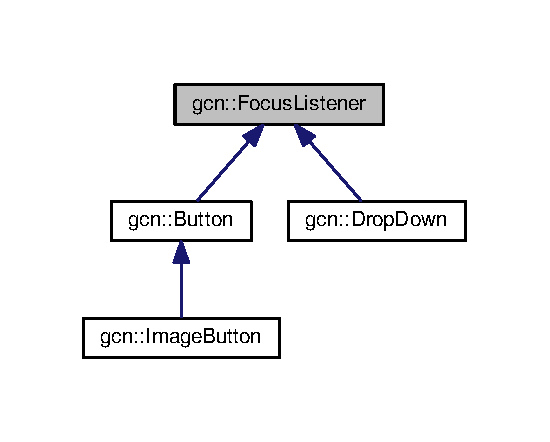
\includegraphics[width=264pt]{classgcn_1_1FocusListener__inherit__graph}
\end{center}
\end{figure}
\subsection*{Public Member Functions}
\begin{DoxyCompactItemize}
\item 
virtual \hyperlink{classgcn_1_1FocusListener_a0590fe4d6d7c97e048e0970f0663620f}{$\sim$\+Focus\+Listener} ()
\item 
virtual void \hyperlink{classgcn_1_1FocusListener_a356aa939465d4916ecaa080df4521711}{focus\+Gained} (const \hyperlink{classgcn_1_1Event}{Event} \&event)
\item 
virtual void \hyperlink{classgcn_1_1FocusListener_a7523032b39888503179e8142d2433b45}{focus\+Lost} (const \hyperlink{classgcn_1_1Event}{Event} \&event)
\end{DoxyCompactItemize}


\subsection{Detailed Description}
Listener of focus events from Widgets. To be able to listen for focus events you must make a class which inherits from this class and implements it\textquotesingle{}s functions.

\begin{DoxySeeAlso}{See also}
\hyperlink{classgcn_1_1Widget_aa6aaaf472d2a562ea101ad1e407ded60}{Widget\+::add\+Focus\+Listener} 
\end{DoxySeeAlso}
\begin{DoxyAuthor}{Author}
Olof Naess�n 
\end{DoxyAuthor}
\begin{DoxySince}{Since}
0.\+7.\+0 
\end{DoxySince}


\subsection{Constructor \& Destructor Documentation}
\index{gcn\+::\+Focus\+Listener@{gcn\+::\+Focus\+Listener}!````~Focus\+Listener@{$\sim$\+Focus\+Listener}}
\index{````~Focus\+Listener@{$\sim$\+Focus\+Listener}!gcn\+::\+Focus\+Listener@{gcn\+::\+Focus\+Listener}}
\subsubsection[{\texorpdfstring{$\sim$\+Focus\+Listener()}{~FocusListener()}}]{\setlength{\rightskip}{0pt plus 5cm}virtual gcn\+::\+Focus\+Listener\+::$\sim$\+Focus\+Listener (
\begin{DoxyParamCaption}
{}
\end{DoxyParamCaption}
)\hspace{0.3cm}{\ttfamily [inline]}, {\ttfamily [virtual]}}\hypertarget{classgcn_1_1FocusListener_a0590fe4d6d7c97e048e0970f0663620f}{}\label{classgcn_1_1FocusListener_a0590fe4d6d7c97e048e0970f0663620f}
Destructor. 

\subsection{Member Function Documentation}
\index{gcn\+::\+Focus\+Listener@{gcn\+::\+Focus\+Listener}!focus\+Gained@{focus\+Gained}}
\index{focus\+Gained@{focus\+Gained}!gcn\+::\+Focus\+Listener@{gcn\+::\+Focus\+Listener}}
\subsubsection[{\texorpdfstring{focus\+Gained(const Event \&event)}{focusGained(const Event &event)}}]{\setlength{\rightskip}{0pt plus 5cm}virtual void gcn\+::\+Focus\+Listener\+::focus\+Gained (
\begin{DoxyParamCaption}
\item[{const {\bf Event} \&}]{event}
\end{DoxyParamCaption}
)\hspace{0.3cm}{\ttfamily [inline]}, {\ttfamily [virtual]}}\hypertarget{classgcn_1_1FocusListener_a356aa939465d4916ecaa080df4521711}{}\label{classgcn_1_1FocusListener_a356aa939465d4916ecaa080df4521711}
Called when a widget gains focus.


\begin{DoxyParams}{Parameters}
{\em event} & discribes the event. \\
\hline
\end{DoxyParams}
\index{gcn\+::\+Focus\+Listener@{gcn\+::\+Focus\+Listener}!focus\+Lost@{focus\+Lost}}
\index{focus\+Lost@{focus\+Lost}!gcn\+::\+Focus\+Listener@{gcn\+::\+Focus\+Listener}}
\subsubsection[{\texorpdfstring{focus\+Lost(const Event \&event)}{focusLost(const Event &event)}}]{\setlength{\rightskip}{0pt plus 5cm}virtual void gcn\+::\+Focus\+Listener\+::focus\+Lost (
\begin{DoxyParamCaption}
\item[{const {\bf Event} \&}]{event}
\end{DoxyParamCaption}
)\hspace{0.3cm}{\ttfamily [inline]}, {\ttfamily [virtual]}}\hypertarget{classgcn_1_1FocusListener_a7523032b39888503179e8142d2433b45}{}\label{classgcn_1_1FocusListener_a7523032b39888503179e8142d2433b45}
Called when a widget loses focus.


\begin{DoxyParams}{Parameters}
{\em event} & discribes the event. \\
\hline
\end{DoxyParams}


Reimplemented in \hyperlink{classgcn_1_1DropDown_a688cf78090ce646ea35e1ca00a441b12}{gcn\+::\+Drop\+Down}, and \hyperlink{classgcn_1_1Button_a6cee079024ffd4e8eeb8b682aade93c0}{gcn\+::\+Button}.



The documentation for this class was generated from the following file\+:\begin{DoxyCompactItemize}
\item 
include/guisan/focuslistener.\+hpp\end{DoxyCompactItemize}

\hypertarget{classgcn_1_1Font}{}\section{gcn\+:\+:Font Class Reference}
\label{classgcn_1_1Font}\index{gcn\+::\+Font@{gcn\+::\+Font}}


{\ttfamily \#include $<$font.\+hpp$>$}



Inheritance diagram for gcn\+:\+:Font\+:\nopagebreak
\begin{figure}[H]
\begin{center}
\leavevmode
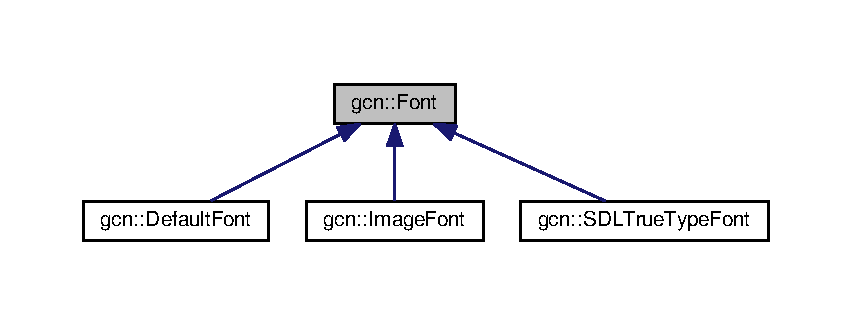
\includegraphics[width=350pt]{classgcn_1_1Font__inherit__graph}
\end{center}
\end{figure}
\subsection*{Public Member Functions}
\begin{DoxyCompactItemize}
\item 
virtual \hyperlink{classgcn_1_1Font_ab3bd1c57c092fe0ad1d027c4076e463d}{$\sim$\+Font} ()
\item 
virtual int \hyperlink{classgcn_1_1Font_abb88894b1ebeda28edcac75c537f8e0f}{get\+Width} (const std\+::string \&text) const =0
\item 
virtual int \hyperlink{classgcn_1_1Font_aa270d8934a16d4065143e3617b1fa926}{get\+Height} () const =0
\item 
virtual int \hyperlink{classgcn_1_1Font_a3210f4c53424ade4b188b8dfb1f686a4}{get\+String\+Index\+At} (const std\+::string \&text, int x)
\item 
virtual void \hyperlink{classgcn_1_1Font_a055c403050f483cc2c67477443d98eee}{draw\+String} (\hyperlink{classgcn_1_1Graphics}{Graphics} $\ast$graphics, const std\+::string \&text, int x, int y)=0
\end{DoxyCompactItemize}


\subsection{Detailed Description}
Holder of a font. Fonts should inherit from this class and implements it\textquotesingle{}s functions.

\begin{DoxySeeAlso}{See also}
\hyperlink{classgcn_1_1ImageFont}{Image\+Font} 
\end{DoxySeeAlso}


\subsection{Constructor \& Destructor Documentation}
\index{gcn\+::\+Font@{gcn\+::\+Font}!````~Font@{$\sim$\+Font}}
\index{````~Font@{$\sim$\+Font}!gcn\+::\+Font@{gcn\+::\+Font}}
\subsubsection[{\texorpdfstring{$\sim$\+Font()}{~Font()}}]{\setlength{\rightskip}{0pt plus 5cm}virtual gcn\+::\+Font\+::$\sim$\+Font (
\begin{DoxyParamCaption}
{}
\end{DoxyParamCaption}
)\hspace{0.3cm}{\ttfamily [inline]}, {\ttfamily [virtual]}}\hypertarget{classgcn_1_1Font_ab3bd1c57c092fe0ad1d027c4076e463d}{}\label{classgcn_1_1Font_ab3bd1c57c092fe0ad1d027c4076e463d}
Destructor. 

\subsection{Member Function Documentation}
\index{gcn\+::\+Font@{gcn\+::\+Font}!draw\+String@{draw\+String}}
\index{draw\+String@{draw\+String}!gcn\+::\+Font@{gcn\+::\+Font}}
\subsubsection[{\texorpdfstring{draw\+String(\+Graphics $\ast$graphics, const std\+::string \&text, int x, int y)=0}{drawString(Graphics *graphics, const std::string &text, int x, int y)=0}}]{\setlength{\rightskip}{0pt plus 5cm}virtual void gcn\+::\+Font\+::draw\+String (
\begin{DoxyParamCaption}
\item[{{\bf Graphics} $\ast$}]{graphics, }
\item[{const std\+::string \&}]{text, }
\item[{int}]{x, }
\item[{int}]{y}
\end{DoxyParamCaption}
)\hspace{0.3cm}{\ttfamily [pure virtual]}}\hypertarget{classgcn_1_1Font_a055c403050f483cc2c67477443d98eee}{}\label{classgcn_1_1Font_a055c403050f483cc2c67477443d98eee}
Draws a string.

N\+O\+TE\+: You normally won\textquotesingle{}t use this function to draw text since \hyperlink{classgcn_1_1Graphics}{Graphics} contains better functions for drawing text.


\begin{DoxyParams}{Parameters}
{\em graphics} & a \hyperlink{classgcn_1_1Graphics}{Graphics} object to use for drawing. \\
\hline
{\em text} & the string to draw. \\
\hline
{\em x} & the x coordinate where to draw the string. \\
\hline
{\em y} & the y coordinate where to draw the string. \\
\hline
\end{DoxyParams}


Implemented in \hyperlink{classgcn_1_1ImageFont_a8717f4ef08e2ba1a1379a4b8fe4b5002}{gcn\+::\+Image\+Font}, \hyperlink{classgcn_1_1SDLTrueTypeFont_a15bd720b4412b4fb49080bc1fd38a363}{gcn\+::\+S\+D\+L\+True\+Type\+Font}, and \hyperlink{classgcn_1_1DefaultFont_a3cdd4f449bd2114312df6970c6ae2571}{gcn\+::\+Default\+Font}.

\index{gcn\+::\+Font@{gcn\+::\+Font}!get\+Height@{get\+Height}}
\index{get\+Height@{get\+Height}!gcn\+::\+Font@{gcn\+::\+Font}}
\subsubsection[{\texorpdfstring{get\+Height() const =0}{getHeight() const =0}}]{\setlength{\rightskip}{0pt plus 5cm}virtual int gcn\+::\+Font\+::get\+Height (
\begin{DoxyParamCaption}
{}
\end{DoxyParamCaption}
) const\hspace{0.3cm}{\ttfamily [pure virtual]}}\hypertarget{classgcn_1_1Font_aa270d8934a16d4065143e3617b1fa926}{}\label{classgcn_1_1Font_aa270d8934a16d4065143e3617b1fa926}
Gets the height of the glyphs in the font.

\begin{DoxyReturn}{Returns}
the height of the glyphs int the font. 
\end{DoxyReturn}


Implemented in \hyperlink{classgcn_1_1ImageFont_ae18f2d854e42ce5aafd44e8b8c6ff048}{gcn\+::\+Image\+Font}, \hyperlink{classgcn_1_1SDLTrueTypeFont_aded39281128e4543eaf2d2e0e858f9a6}{gcn\+::\+S\+D\+L\+True\+Type\+Font}, and \hyperlink{classgcn_1_1DefaultFont_a64f2f7bcce5d3780106634e36ac0a52a}{gcn\+::\+Default\+Font}.

\index{gcn\+::\+Font@{gcn\+::\+Font}!get\+String\+Index\+At@{get\+String\+Index\+At}}
\index{get\+String\+Index\+At@{get\+String\+Index\+At}!gcn\+::\+Font@{gcn\+::\+Font}}
\subsubsection[{\texorpdfstring{get\+String\+Index\+At(const std\+::string \&text, int x)}{getStringIndexAt(const std::string &text, int x)}}]{\setlength{\rightskip}{0pt plus 5cm}int gcn\+::\+Font\+::get\+String\+Index\+At (
\begin{DoxyParamCaption}
\item[{const std\+::string \&}]{text, }
\item[{int}]{x}
\end{DoxyParamCaption}
)\hspace{0.3cm}{\ttfamily [virtual]}}\hypertarget{classgcn_1_1Font_a3210f4c53424ade4b188b8dfb1f686a4}{}\label{classgcn_1_1Font_a3210f4c53424ade4b188b8dfb1f686a4}
Gets a string index in a string providing an x coordinate. Used to retrive a string index (for a character in a string) at a certain x position. It is especially useful when a mouse clicks in a \hyperlink{classgcn_1_1TextField}{Text\+Field} and you want to know which character was clicked.

\begin{DoxyReturn}{Returns}
a string index in a string providing an x coordinate. 
\end{DoxyReturn}


Reimplemented in \hyperlink{classgcn_1_1ImageFont_a5b0e7a7a7acdcb9fadb232f63608b354}{gcn\+::\+Image\+Font}, and \hyperlink{classgcn_1_1DefaultFont_a10b802c51de668171c2255f2e11fc063}{gcn\+::\+Default\+Font}.

\index{gcn\+::\+Font@{gcn\+::\+Font}!get\+Width@{get\+Width}}
\index{get\+Width@{get\+Width}!gcn\+::\+Font@{gcn\+::\+Font}}
\subsubsection[{\texorpdfstring{get\+Width(const std\+::string \&text) const =0}{getWidth(const std::string &text) const =0}}]{\setlength{\rightskip}{0pt plus 5cm}virtual int gcn\+::\+Font\+::get\+Width (
\begin{DoxyParamCaption}
\item[{const std\+::string \&}]{text}
\end{DoxyParamCaption}
) const\hspace{0.3cm}{\ttfamily [pure virtual]}}\hypertarget{classgcn_1_1Font_abb88894b1ebeda28edcac75c537f8e0f}{}\label{classgcn_1_1Font_abb88894b1ebeda28edcac75c537f8e0f}
Gets the width of a string. The width of a string is not necesserily the sum of all the widths of it\textquotesingle{}s glyphs.


\begin{DoxyParams}{Parameters}
{\em text} & the string to return the width of. \\
\hline
\end{DoxyParams}
\begin{DoxyReturn}{Returns}
the width of a string. 
\end{DoxyReturn}


Implemented in \hyperlink{classgcn_1_1ImageFont_a6432c448c9df16a3ca057b2bd9822663}{gcn\+::\+Image\+Font}, \hyperlink{classgcn_1_1SDLTrueTypeFont_a3389cfeda7002e3888be2731ff8560d7}{gcn\+::\+S\+D\+L\+True\+Type\+Font}, and \hyperlink{classgcn_1_1DefaultFont_a62d609afe7f0d0dec90a0ae1cb4731ea}{gcn\+::\+Default\+Font}.



The documentation for this class was generated from the following files\+:\begin{DoxyCompactItemize}
\item 
include/guisan/font.\+hpp\item 
src/font.\+cpp\end{DoxyCompactItemize}

\hypertarget{classgcn_1_1GenericInput}{}\section{gcn\+:\+:Generic\+Input Class Reference}
\label{classgcn_1_1GenericInput}\index{gcn\+::\+Generic\+Input@{gcn\+::\+Generic\+Input}}


{\ttfamily \#include $<$genericinput.\+hpp$>$}



Inheritance diagram for gcn\+:\+:Generic\+Input\+:\nopagebreak
\begin{figure}[H]
\begin{center}
\leavevmode
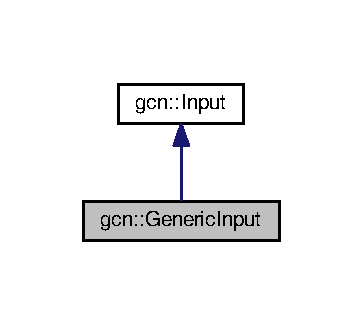
\includegraphics[width=174pt]{classgcn_1_1GenericInput__inherit__graph}
\end{center}
\end{figure}


Collaboration diagram for gcn\+:\+:Generic\+Input\+:\nopagebreak
\begin{figure}[H]
\begin{center}
\leavevmode
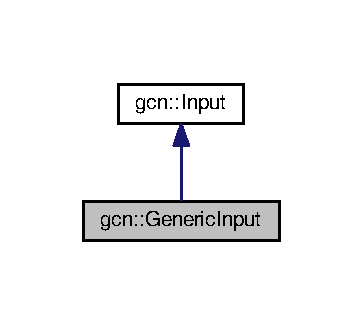
\includegraphics[width=174pt]{classgcn_1_1GenericInput__coll__graph}
\end{center}
\end{figure}
\subsection*{Public Member Functions}
\begin{DoxyCompactItemize}
\item 
\hyperlink{classgcn_1_1GenericInput_a5faf6486010b0c13c14ac2d80fc05609}{Generic\+Input} ()
\item 
void \hyperlink{classgcn_1_1GenericInput_a347258d8ee30fe5637f5eeb1e15e8eb4}{push\+Key\+Pressed} (int unicode)
\item 
void \hyperlink{classgcn_1_1GenericInput_a8db8d150eef492434df647351731dbe3}{push\+Key\+Released} (int unicode)
\item 
void \hyperlink{classgcn_1_1GenericInput_af951a9c1b061685a6f653ba01b4abb73}{push\+Mouse\+Button\+Pressed} (int x, int y, int button)
\item 
void \hyperlink{classgcn_1_1GenericInput_a87a8597cb766115cddca7844df852ba4}{push\+Mouse\+Button\+Released} (int x, int y, int button)
\item 
void \hyperlink{classgcn_1_1GenericInput_a7e070cf0ce34e720519b427489fdb86a}{push\+Mouse\+Wheel\+Moved\+Up} (int x, int y)
\item 
void \hyperlink{classgcn_1_1GenericInput_ab0a4399fe1487dc8355f4a6ce5c3d6d1}{push\+Mouse\+Wheel\+Moved\+Down} (int x, int y)
\item 
void \hyperlink{classgcn_1_1GenericInput_aa07fa9d97d110e0d5e97763112e156d8}{push\+Mouse\+Moved} (int x, int y)
\item 
virtual bool \hyperlink{classgcn_1_1GenericInput_a095d139685ca11045a3f6d8041fe97f1}{is\+Key\+Queue\+Empty} ()
\item 
virtual \hyperlink{classgcn_1_1KeyInput}{Key\+Input} \hyperlink{classgcn_1_1GenericInput_a2a1ee4f5f85ec92e2d79e96a394c7880}{dequeue\+Key\+Input} ()
\item 
virtual bool \hyperlink{classgcn_1_1GenericInput_a67de2fb91e717d67b018fea8243ecd3d}{is\+Mouse\+Queue\+Empty} ()
\item 
virtual \hyperlink{classgcn_1_1MouseInput}{Mouse\+Input} \hyperlink{classgcn_1_1GenericInput_acdc29660e3b837cd9152d99a7457dcd1}{dequeue\+Mouse\+Input} ()
\item 
virtual void \hyperlink{classgcn_1_1GenericInput_aaa13d9c4a0c39efcf5ff18aeecfd5f86}{\+\_\+poll\+Input} ()
\end{DoxyCompactItemize}
\subsection*{Protected Attributes}
\begin{DoxyCompactItemize}
\item 
std\+::queue$<$ \hyperlink{classgcn_1_1KeyInput}{Key\+Input} $>$ {\bfseries m\+Key\+Input\+Queue}\hypertarget{classgcn_1_1GenericInput_aa324311178de5455719b754fe05ac059}{}\label{classgcn_1_1GenericInput_aa324311178de5455719b754fe05ac059}

\item 
std\+::queue$<$ \hyperlink{classgcn_1_1MouseInput}{Mouse\+Input} $>$ {\bfseries m\+Mouse\+Input\+Queue}\hypertarget{classgcn_1_1GenericInput_a6403fa3f08d98d46e9edf4f666e419df}{}\label{classgcn_1_1GenericInput_a6403fa3f08d98d46e9edf4f666e419df}

\end{DoxyCompactItemize}


\subsection{Detailed Description}
Generic input which can be used with any backend. 

\subsection{Constructor \& Destructor Documentation}
\index{gcn\+::\+Generic\+Input@{gcn\+::\+Generic\+Input}!Generic\+Input@{Generic\+Input}}
\index{Generic\+Input@{Generic\+Input}!gcn\+::\+Generic\+Input@{gcn\+::\+Generic\+Input}}
\subsubsection[{\texorpdfstring{Generic\+Input()}{GenericInput()}}]{\setlength{\rightskip}{0pt plus 5cm}gcn\+::\+Generic\+Input\+::\+Generic\+Input (
\begin{DoxyParamCaption}
{}
\end{DoxyParamCaption}
)}\hypertarget{classgcn_1_1GenericInput_a5faf6486010b0c13c14ac2d80fc05609}{}\label{classgcn_1_1GenericInput_a5faf6486010b0c13c14ac2d80fc05609}
Constructor. 

\subsection{Member Function Documentation}
\index{gcn\+::\+Generic\+Input@{gcn\+::\+Generic\+Input}!\+\_\+poll\+Input@{\+\_\+poll\+Input}}
\index{\+\_\+poll\+Input@{\+\_\+poll\+Input}!gcn\+::\+Generic\+Input@{gcn\+::\+Generic\+Input}}
\subsubsection[{\texorpdfstring{\+\_\+poll\+Input()}{_pollInput()}}]{\setlength{\rightskip}{0pt plus 5cm}void gcn\+::\+Generic\+Input\+::\+\_\+poll\+Input (
\begin{DoxyParamCaption}
{}
\end{DoxyParamCaption}
)\hspace{0.3cm}{\ttfamily [virtual]}}\hypertarget{classgcn_1_1GenericInput_aaa13d9c4a0c39efcf5ff18aeecfd5f86}{}\label{classgcn_1_1GenericInput_aaa13d9c4a0c39efcf5ff18aeecfd5f86}
Polls all exsisting input. It exists for \hyperlink{classgcn_1_1Input}{Input} implementation compatibility. It is used internally by the library. 

Implements \hyperlink{classgcn_1_1Input_a8e852901ad206985f18ae25e99867cb6}{gcn\+::\+Input}.

\index{gcn\+::\+Generic\+Input@{gcn\+::\+Generic\+Input}!dequeue\+Key\+Input@{dequeue\+Key\+Input}}
\index{dequeue\+Key\+Input@{dequeue\+Key\+Input}!gcn\+::\+Generic\+Input@{gcn\+::\+Generic\+Input}}
\subsubsection[{\texorpdfstring{dequeue\+Key\+Input()}{dequeueKeyInput()}}]{\setlength{\rightskip}{0pt plus 5cm}{\bf Key\+Input} gcn\+::\+Generic\+Input\+::dequeue\+Key\+Input (
\begin{DoxyParamCaption}
{}
\end{DoxyParamCaption}
)\hspace{0.3cm}{\ttfamily [virtual]}}\hypertarget{classgcn_1_1GenericInput_a2a1ee4f5f85ec92e2d79e96a394c7880}{}\label{classgcn_1_1GenericInput_a2a1ee4f5f85ec92e2d79e96a394c7880}
Dequeues the key input queue.

\begin{DoxyReturn}{Returns}
key input. 
\end{DoxyReturn}


Implements \hyperlink{classgcn_1_1Input_a3c4c2e5a0328dff6f90d81fb22e30d6c}{gcn\+::\+Input}.

\index{gcn\+::\+Generic\+Input@{gcn\+::\+Generic\+Input}!dequeue\+Mouse\+Input@{dequeue\+Mouse\+Input}}
\index{dequeue\+Mouse\+Input@{dequeue\+Mouse\+Input}!gcn\+::\+Generic\+Input@{gcn\+::\+Generic\+Input}}
\subsubsection[{\texorpdfstring{dequeue\+Mouse\+Input()}{dequeueMouseInput()}}]{\setlength{\rightskip}{0pt plus 5cm}{\bf Mouse\+Input} gcn\+::\+Generic\+Input\+::dequeue\+Mouse\+Input (
\begin{DoxyParamCaption}
{}
\end{DoxyParamCaption}
)\hspace{0.3cm}{\ttfamily [virtual]}}\hypertarget{classgcn_1_1GenericInput_acdc29660e3b837cd9152d99a7457dcd1}{}\label{classgcn_1_1GenericInput_acdc29660e3b837cd9152d99a7457dcd1}
Dequeues the mouse input queue.

\begin{DoxyReturn}{Returns}
mouse input. 
\end{DoxyReturn}


Implements \hyperlink{classgcn_1_1Input_a974c5ffa91c1f80185f32ac10a5de3e2}{gcn\+::\+Input}.

\index{gcn\+::\+Generic\+Input@{gcn\+::\+Generic\+Input}!is\+Key\+Queue\+Empty@{is\+Key\+Queue\+Empty}}
\index{is\+Key\+Queue\+Empty@{is\+Key\+Queue\+Empty}!gcn\+::\+Generic\+Input@{gcn\+::\+Generic\+Input}}
\subsubsection[{\texorpdfstring{is\+Key\+Queue\+Empty()}{isKeyQueueEmpty()}}]{\setlength{\rightskip}{0pt plus 5cm}bool gcn\+::\+Generic\+Input\+::is\+Key\+Queue\+Empty (
\begin{DoxyParamCaption}
{}
\end{DoxyParamCaption}
)\hspace{0.3cm}{\ttfamily [virtual]}}\hypertarget{classgcn_1_1GenericInput_a095d139685ca11045a3f6d8041fe97f1}{}\label{classgcn_1_1GenericInput_a095d139685ca11045a3f6d8041fe97f1}
Checks whether the key queue is empty or not.

\begin{DoxyReturn}{Returns}
true if the key queue is empty. 
\end{DoxyReturn}


Implements \hyperlink{classgcn_1_1Input_a99c69c2e8d9b4378c4cea1f8beed0cf3}{gcn\+::\+Input}.

\index{gcn\+::\+Generic\+Input@{gcn\+::\+Generic\+Input}!is\+Mouse\+Queue\+Empty@{is\+Mouse\+Queue\+Empty}}
\index{is\+Mouse\+Queue\+Empty@{is\+Mouse\+Queue\+Empty}!gcn\+::\+Generic\+Input@{gcn\+::\+Generic\+Input}}
\subsubsection[{\texorpdfstring{is\+Mouse\+Queue\+Empty()}{isMouseQueueEmpty()}}]{\setlength{\rightskip}{0pt plus 5cm}bool gcn\+::\+Generic\+Input\+::is\+Mouse\+Queue\+Empty (
\begin{DoxyParamCaption}
{}
\end{DoxyParamCaption}
)\hspace{0.3cm}{\ttfamily [virtual]}}\hypertarget{classgcn_1_1GenericInput_a67de2fb91e717d67b018fea8243ecd3d}{}\label{classgcn_1_1GenericInput_a67de2fb91e717d67b018fea8243ecd3d}
Checks whether the mouse queue is empyt or not.

\begin{DoxyReturn}{Returns}
true if the mouse queue is empty. 
\end{DoxyReturn}


Implements \hyperlink{classgcn_1_1Input_a9c59ac0d0ae6c2eb4967f3eb6d9e059f}{gcn\+::\+Input}.

\index{gcn\+::\+Generic\+Input@{gcn\+::\+Generic\+Input}!push\+Key\+Pressed@{push\+Key\+Pressed}}
\index{push\+Key\+Pressed@{push\+Key\+Pressed}!gcn\+::\+Generic\+Input@{gcn\+::\+Generic\+Input}}
\subsubsection[{\texorpdfstring{push\+Key\+Pressed(int unicode)}{pushKeyPressed(int unicode)}}]{\setlength{\rightskip}{0pt plus 5cm}void gcn\+::\+Generic\+Input\+::push\+Key\+Pressed (
\begin{DoxyParamCaption}
\item[{int}]{unicode}
\end{DoxyParamCaption}
)}\hypertarget{classgcn_1_1GenericInput_a347258d8ee30fe5637f5eeb1e15e8eb4}{}\label{classgcn_1_1GenericInput_a347258d8ee30fe5637f5eeb1e15e8eb4}
Pushes a key pressed event.

N\+O\+TE\+: If a special key is pressed, like the F1 key, the corresponding Guichan key value found in the enum in \hyperlink{classgcn_1_1Key}{Key} should be pushed as the unicode value.


\begin{DoxyParams}{Parameters}
{\em unicode} & the unicode value of the key. \\
\hline
\end{DoxyParams}
\index{gcn\+::\+Generic\+Input@{gcn\+::\+Generic\+Input}!push\+Key\+Released@{push\+Key\+Released}}
\index{push\+Key\+Released@{push\+Key\+Released}!gcn\+::\+Generic\+Input@{gcn\+::\+Generic\+Input}}
\subsubsection[{\texorpdfstring{push\+Key\+Released(int unicode)}{pushKeyReleased(int unicode)}}]{\setlength{\rightskip}{0pt plus 5cm}void gcn\+::\+Generic\+Input\+::push\+Key\+Released (
\begin{DoxyParamCaption}
\item[{int}]{unicode}
\end{DoxyParamCaption}
)}\hypertarget{classgcn_1_1GenericInput_a8db8d150eef492434df647351731dbe3}{}\label{classgcn_1_1GenericInput_a8db8d150eef492434df647351731dbe3}
Pushes a key released event.

N\+O\+TE\+: If a special key is pressed, like the F1 key, the corresponding Guichan key value found in the enum in \hyperlink{classgcn_1_1Key}{Key} should be pushed as the unicode value.


\begin{DoxyParams}{Parameters}
{\em unicode} & the unicode value of the key. \\
\hline
\end{DoxyParams}
\index{gcn\+::\+Generic\+Input@{gcn\+::\+Generic\+Input}!push\+Mouse\+Button\+Pressed@{push\+Mouse\+Button\+Pressed}}
\index{push\+Mouse\+Button\+Pressed@{push\+Mouse\+Button\+Pressed}!gcn\+::\+Generic\+Input@{gcn\+::\+Generic\+Input}}
\subsubsection[{\texorpdfstring{push\+Mouse\+Button\+Pressed(int x, int y, int button)}{pushMouseButtonPressed(int x, int y, int button)}}]{\setlength{\rightskip}{0pt plus 5cm}void gcn\+::\+Generic\+Input\+::push\+Mouse\+Button\+Pressed (
\begin{DoxyParamCaption}
\item[{int}]{x, }
\item[{int}]{y, }
\item[{int}]{button}
\end{DoxyParamCaption}
)}\hypertarget{classgcn_1_1GenericInput_af951a9c1b061685a6f653ba01b4abb73}{}\label{classgcn_1_1GenericInput_af951a9c1b061685a6f653ba01b4abb73}
Pushes a mouse button pressed event.


\begin{DoxyParams}{Parameters}
{\em x} & the x coordinate of the mouse event. \\
\hline
{\em y} & the y coordinate of the mouse event. \\
\hline
{\em button} & the button of the mouse event. \\
\hline
\end{DoxyParams}
\index{gcn\+::\+Generic\+Input@{gcn\+::\+Generic\+Input}!push\+Mouse\+Button\+Released@{push\+Mouse\+Button\+Released}}
\index{push\+Mouse\+Button\+Released@{push\+Mouse\+Button\+Released}!gcn\+::\+Generic\+Input@{gcn\+::\+Generic\+Input}}
\subsubsection[{\texorpdfstring{push\+Mouse\+Button\+Released(int x, int y, int button)}{pushMouseButtonReleased(int x, int y, int button)}}]{\setlength{\rightskip}{0pt plus 5cm}void gcn\+::\+Generic\+Input\+::push\+Mouse\+Button\+Released (
\begin{DoxyParamCaption}
\item[{int}]{x, }
\item[{int}]{y, }
\item[{int}]{button}
\end{DoxyParamCaption}
)}\hypertarget{classgcn_1_1GenericInput_a87a8597cb766115cddca7844df852ba4}{}\label{classgcn_1_1GenericInput_a87a8597cb766115cddca7844df852ba4}
Pushes a mouse button released event.


\begin{DoxyParams}{Parameters}
{\em x} & the x coordinate of the mouse event. \\
\hline
{\em y} & the y coordinate of the mouse event. \\
\hline
{\em button} & the button of the mouse event. \\
\hline
\end{DoxyParams}
\index{gcn\+::\+Generic\+Input@{gcn\+::\+Generic\+Input}!push\+Mouse\+Moved@{push\+Mouse\+Moved}}
\index{push\+Mouse\+Moved@{push\+Mouse\+Moved}!gcn\+::\+Generic\+Input@{gcn\+::\+Generic\+Input}}
\subsubsection[{\texorpdfstring{push\+Mouse\+Moved(int x, int y)}{pushMouseMoved(int x, int y)}}]{\setlength{\rightskip}{0pt plus 5cm}void gcn\+::\+Generic\+Input\+::push\+Mouse\+Moved (
\begin{DoxyParamCaption}
\item[{int}]{x, }
\item[{int}]{y}
\end{DoxyParamCaption}
)}\hypertarget{classgcn_1_1GenericInput_aa07fa9d97d110e0d5e97763112e156d8}{}\label{classgcn_1_1GenericInput_aa07fa9d97d110e0d5e97763112e156d8}
Pushes a mouse moved event.


\begin{DoxyParams}{Parameters}
{\em x} & the x coordinate of the mouse event. \\
\hline
{\em y} & the y coordinate of the mouse event. \\
\hline
\end{DoxyParams}
\index{gcn\+::\+Generic\+Input@{gcn\+::\+Generic\+Input}!push\+Mouse\+Wheel\+Moved\+Down@{push\+Mouse\+Wheel\+Moved\+Down}}
\index{push\+Mouse\+Wheel\+Moved\+Down@{push\+Mouse\+Wheel\+Moved\+Down}!gcn\+::\+Generic\+Input@{gcn\+::\+Generic\+Input}}
\subsubsection[{\texorpdfstring{push\+Mouse\+Wheel\+Moved\+Down(int x, int y)}{pushMouseWheelMovedDown(int x, int y)}}]{\setlength{\rightskip}{0pt plus 5cm}void gcn\+::\+Generic\+Input\+::push\+Mouse\+Wheel\+Moved\+Down (
\begin{DoxyParamCaption}
\item[{int}]{x, }
\item[{int}]{y}
\end{DoxyParamCaption}
)}\hypertarget{classgcn_1_1GenericInput_ab0a4399fe1487dc8355f4a6ce5c3d6d1}{}\label{classgcn_1_1GenericInput_ab0a4399fe1487dc8355f4a6ce5c3d6d1}
Pushes a mouse wheel moved down event.


\begin{DoxyParams}{Parameters}
{\em x} & the x coordinate of the mouse event. \\
\hline
{\em y} & the y coordinate of the mouse event. \\
\hline
\end{DoxyParams}
\index{gcn\+::\+Generic\+Input@{gcn\+::\+Generic\+Input}!push\+Mouse\+Wheel\+Moved\+Up@{push\+Mouse\+Wheel\+Moved\+Up}}
\index{push\+Mouse\+Wheel\+Moved\+Up@{push\+Mouse\+Wheel\+Moved\+Up}!gcn\+::\+Generic\+Input@{gcn\+::\+Generic\+Input}}
\subsubsection[{\texorpdfstring{push\+Mouse\+Wheel\+Moved\+Up(int x, int y)}{pushMouseWheelMovedUp(int x, int y)}}]{\setlength{\rightskip}{0pt plus 5cm}void gcn\+::\+Generic\+Input\+::push\+Mouse\+Wheel\+Moved\+Up (
\begin{DoxyParamCaption}
\item[{int}]{x, }
\item[{int}]{y}
\end{DoxyParamCaption}
)}\hypertarget{classgcn_1_1GenericInput_a7e070cf0ce34e720519b427489fdb86a}{}\label{classgcn_1_1GenericInput_a7e070cf0ce34e720519b427489fdb86a}
Pushes a mouse wheel moved up event.


\begin{DoxyParams}{Parameters}
{\em x} & the x coordinate of the mouse event. \\
\hline
{\em y} & the y coordinate of the mouse event. \\
\hline
\end{DoxyParams}


The documentation for this class was generated from the following files\+:\begin{DoxyCompactItemize}
\item 
include/guisan/genericinput.\+hpp\item 
src/genericinput.\+cpp\end{DoxyCompactItemize}

\hypertarget{classgcn_1_1Graphics}{}\section{gcn\+:\+:Graphics Class Reference}
\label{classgcn_1_1Graphics}\index{gcn\+::\+Graphics@{gcn\+::\+Graphics}}


{\ttfamily \#include $<$graphics.\+hpp$>$}



Inheritance diagram for gcn\+:\+:Graphics\+:\nopagebreak
\begin{figure}[H]
\begin{center}
\leavevmode
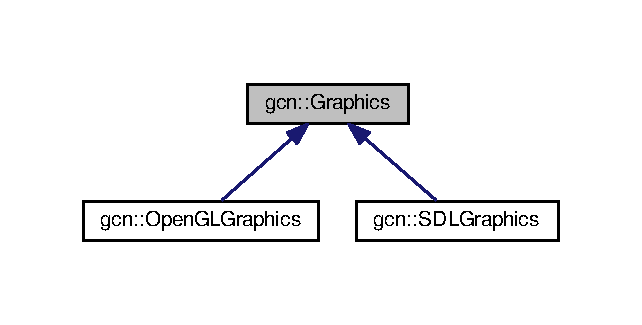
\includegraphics[width=308pt]{classgcn_1_1Graphics__inherit__graph}
\end{center}
\end{figure}


Collaboration diagram for gcn\+:\+:Graphics\+:\nopagebreak
\begin{figure}[H]
\begin{center}
\leavevmode
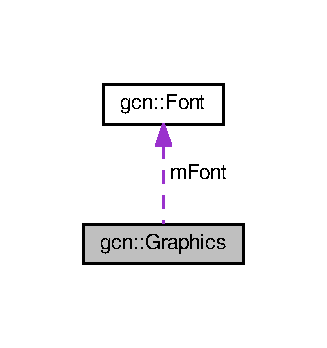
\includegraphics[width=157pt]{classgcn_1_1Graphics__coll__graph}
\end{center}
\end{figure}
\subsection*{Public Types}
\begin{DoxyCompactItemize}
\item 
enum \{ {\bfseries L\+E\+FT} = 0, 
{\bfseries C\+E\+N\+T\+ER}, 
{\bfseries R\+I\+G\+HT}
 \}
\end{DoxyCompactItemize}
\subsection*{Public Member Functions}
\begin{DoxyCompactItemize}
\item 
virtual void \hyperlink{classgcn_1_1Graphics_a85e8107504f70fa460b844fb2259c653}{\+\_\+begin\+Draw} ()
\item 
virtual void \hyperlink{classgcn_1_1Graphics_af6b9381e34ec34f10e9bbf77b7b00c78}{\+\_\+end\+Draw} ()
\item 
virtual bool \hyperlink{classgcn_1_1Graphics_ab8f8773da6aa70f5fb554c2a2815c496}{push\+Clip\+Area} (\hyperlink{classgcn_1_1Rectangle}{Rectangle} area)
\item 
virtual void \hyperlink{classgcn_1_1Graphics_a11a3be7969db7490df8a02cb4549b443}{pop\+Clip\+Area} ()
\item 
virtual const \hyperlink{classgcn_1_1ClipRectangle}{Clip\+Rectangle} \& \hyperlink{classgcn_1_1Graphics_a642535039e421b0530bd85d71b8f7151}{get\+Current\+Clip\+Area} ()
\item 
virtual void \hyperlink{classgcn_1_1Graphics_aeb284b30f59d5cfa4c4e25130f4c164e}{draw\+Image} (const \hyperlink{classgcn_1_1Image}{Image} $\ast$image, int srcX, int srcY, int dstX, int dstY, int width, int height)=0
\item 
virtual void \hyperlink{classgcn_1_1Graphics_aed30c3aa213a2d225b1c119b3f5f8d60}{draw\+Image} (const \hyperlink{classgcn_1_1Image}{Image} $\ast$image, int dstX, int dstY)
\item 
virtual void \hyperlink{classgcn_1_1Graphics_adfd989a2a8c6771c6368b25f3977ecf4}{draw\+Point} (int x, int y)=0
\item 
virtual void \hyperlink{classgcn_1_1Graphics_a92af7e5f5ed6ebf692803bc1bd1d5db5}{draw\+Line} (int x1, int y1, int x2, int y2)=0
\item 
virtual void \hyperlink{classgcn_1_1Graphics_a8ffb254f53931ce3809a6f10307fcbf2}{draw\+Rectangle} (const \hyperlink{classgcn_1_1Rectangle}{Rectangle} \&rectangle)=0
\item 
virtual void \hyperlink{classgcn_1_1Graphics_a5caac226a94ecf8fdfee1da7cd14f0df}{fill\+Rectangle} (const \hyperlink{classgcn_1_1Rectangle}{Rectangle} \&rectangle)=0
\item 
virtual void \hyperlink{classgcn_1_1Graphics_a7f438ae2b4cc09c66d77a9b9cb591e7c}{set\+Color} (const \hyperlink{classgcn_1_1Color}{Color} \&color)=0
\item 
virtual const \hyperlink{classgcn_1_1Color}{Color} \& \hyperlink{classgcn_1_1Graphics_a509769aaeb7356cd0f595f3ddb962e49}{get\+Color} ()=0
\item 
virtual void \hyperlink{classgcn_1_1Graphics_a7415290eb8b075fae0b4a6fce3912f4e}{set\+Font} (\hyperlink{classgcn_1_1Font}{Font} $\ast$font)
\item 
virtual void \hyperlink{classgcn_1_1Graphics_a664fcd573d3e002d9096abdb8ce3279e}{draw\+Text} (const std\+::string \&text, int x, int y, unsigned int alignment=L\+E\+FT)
\end{DoxyCompactItemize}
\subsection*{Protected Attributes}
\begin{DoxyCompactItemize}
\item 
std\+::stack$<$ \hyperlink{classgcn_1_1ClipRectangle}{Clip\+Rectangle} $>$ {\bfseries m\+Clip\+Stack}\hypertarget{classgcn_1_1Graphics_a08be42a39b774cd0ee449a8cc76cc84b}{}\label{classgcn_1_1Graphics_a08be42a39b774cd0ee449a8cc76cc84b}

\item 
\hyperlink{classgcn_1_1Font}{Font} $\ast$ {\bfseries m\+Font}\hypertarget{classgcn_1_1Graphics_af58494bcfd95382cb7af4f0d573b8b1a}{}\label{classgcn_1_1Graphics_af58494bcfd95382cb7af4f0d573b8b1a}

\end{DoxyCompactItemize}


\subsection{Detailed Description}
Used for drawing graphics. It contains all vital functions for drawing. We include implemented \hyperlink{classgcn_1_1Graphics}{Graphics} classes for some common platforms like the Allegro library, the Open\+GL library and the S\+DL library. To make Guichan usable under another platform, a \hyperlink{classgcn_1_1Graphics}{Graphics} class must be implemented.

In \hyperlink{classgcn_1_1Graphics}{Graphics} you can set clip areas to limit drawing to certain areas of the screen. Clip areas are put on a stack, which means that you can push smaller and smaller clip areas onto the stack. All coordinates will be relative to the topmost clip area. In most cases you won\textquotesingle{}t have to worry about the clip areas, unless you want to implement some really complex widget. Pushing and poping of clip areas are handled automatically by container widgets when their child widgets are drawn.

I\+M\+P\+O\+R\+T\+A\+NT\+: Remember to pop each clip area that you pushed on the stack after you are done with it.

If you feel that \hyperlink{classgcn_1_1Graphics}{Graphics} is to restrictive for your needs, there is no one stopping you from using your own code for drawing in Widgets. You could for instance use pure S\+DL in the drawing of Widgets bypassing \hyperlink{classgcn_1_1Graphics}{Graphics}. This might however hurt portability of your application.

If you implement a \hyperlink{classgcn_1_1Graphics}{Graphics} class not present in Guichan we would be very happy to add it to Guichan.

\begin{DoxySeeAlso}{See also}
Allegro\+Graphics, \hyperlink{classgcn_1_1OpenGLGraphics}{Open\+G\+L\+Graphics}, \hyperlink{classgcn_1_1SDLGraphics}{S\+D\+L\+Graphics}, \hyperlink{classgcn_1_1Image}{Image} 
\end{DoxySeeAlso}


\subsection{Member Enumeration Documentation}
\subsubsection[{\texorpdfstring{anonymous enum}{anonymous enum}}]{\setlength{\rightskip}{0pt plus 5cm}anonymous enum}\hypertarget{classgcn_1_1Graphics_ac99c177417b14be6fc5cdb8cad5d0d76}{}\label{classgcn_1_1Graphics_ac99c177417b14be6fc5cdb8cad5d0d76}
Alignments for text drawing. 

\subsection{Member Function Documentation}
\index{gcn\+::\+Graphics@{gcn\+::\+Graphics}!\+\_\+begin\+Draw@{\+\_\+begin\+Draw}}
\index{\+\_\+begin\+Draw@{\+\_\+begin\+Draw}!gcn\+::\+Graphics@{gcn\+::\+Graphics}}
\subsubsection[{\texorpdfstring{\+\_\+begin\+Draw()}{_beginDraw()}}]{\setlength{\rightskip}{0pt plus 5cm}virtual void gcn\+::\+Graphics\+::\+\_\+begin\+Draw (
\begin{DoxyParamCaption}
{}
\end{DoxyParamCaption}
)\hspace{0.3cm}{\ttfamily [inline]}, {\ttfamily [virtual]}}\hypertarget{classgcn_1_1Graphics_a85e8107504f70fa460b844fb2259c653}{}\label{classgcn_1_1Graphics_a85e8107504f70fa460b844fb2259c653}
Initializes drawing. Called by the \hyperlink{classgcn_1_1Gui}{Gui} when \hyperlink{classgcn_1_1Gui_ad231f982fb8182b16ecf11075054f4ac}{Gui\+::draw()} is called. It is needed by some implementations of \hyperlink{classgcn_1_1Graphics}{Graphics} to perform preparations before drawing. An example of such an implementation would be \hyperlink{classgcn_1_1OpenGLGraphics}{Open\+G\+L\+Graphics}.

N\+O\+TE\+: You will never need to call this function yourself. \hyperlink{classgcn_1_1Gui}{Gui} will do it for you.

\begin{DoxySeeAlso}{See also}
\hyperlink{classgcn_1_1Graphics_af6b9381e34ec34f10e9bbf77b7b00c78}{\+\_\+end\+Draw}, \hyperlink{classgcn_1_1Gui_ad231f982fb8182b16ecf11075054f4ac}{Gui\+::draw} 
\end{DoxySeeAlso}


Reimplemented in \hyperlink{classgcn_1_1SDLGraphics_a8a551d5159bb79dd7d77cd081f5d9c78}{gcn\+::\+S\+D\+L\+Graphics}, and \hyperlink{classgcn_1_1OpenGLGraphics_a48173540d3ea957c6ecb7baeb4e48772}{gcn\+::\+Open\+G\+L\+Graphics}.

\index{gcn\+::\+Graphics@{gcn\+::\+Graphics}!\+\_\+end\+Draw@{\+\_\+end\+Draw}}
\index{\+\_\+end\+Draw@{\+\_\+end\+Draw}!gcn\+::\+Graphics@{gcn\+::\+Graphics}}
\subsubsection[{\texorpdfstring{\+\_\+end\+Draw()}{_endDraw()}}]{\setlength{\rightskip}{0pt plus 5cm}virtual void gcn\+::\+Graphics\+::\+\_\+end\+Draw (
\begin{DoxyParamCaption}
{}
\end{DoxyParamCaption}
)\hspace{0.3cm}{\ttfamily [inline]}, {\ttfamily [virtual]}}\hypertarget{classgcn_1_1Graphics_af6b9381e34ec34f10e9bbf77b7b00c78}{}\label{classgcn_1_1Graphics_af6b9381e34ec34f10e9bbf77b7b00c78}
Deinitializes drawing. Called by the \hyperlink{classgcn_1_1Gui}{Gui} when a \hyperlink{classgcn_1_1Gui_ad231f982fb8182b16ecf11075054f4ac}{Gui\+::draw()} is done. done. It should reset any state changes made by \hyperlink{classgcn_1_1Graphics_a85e8107504f70fa460b844fb2259c653}{\+\_\+begin\+Draw()}.

N\+O\+TE\+: You will never need to call this function yourself. \hyperlink{classgcn_1_1Gui}{Gui} will do it for you.

\begin{DoxySeeAlso}{See also}
\hyperlink{classgcn_1_1Graphics_a85e8107504f70fa460b844fb2259c653}{\+\_\+begin\+Draw}, \hyperlink{classgcn_1_1Gui_ad231f982fb8182b16ecf11075054f4ac}{Gui\+::draw} 
\end{DoxySeeAlso}


Reimplemented in \hyperlink{classgcn_1_1SDLGraphics_a1ec61016736b34271f60e3a88d65c1b7}{gcn\+::\+S\+D\+L\+Graphics}, and \hyperlink{classgcn_1_1OpenGLGraphics_abf1f271776344b1aa28b5eb0faf8bc1d}{gcn\+::\+Open\+G\+L\+Graphics}.

\index{gcn\+::\+Graphics@{gcn\+::\+Graphics}!draw\+Image@{draw\+Image}}
\index{draw\+Image@{draw\+Image}!gcn\+::\+Graphics@{gcn\+::\+Graphics}}
\subsubsection[{\texorpdfstring{draw\+Image(const Image $\ast$image, int src\+X, int src\+Y, int dst\+X, int dst\+Y, int width, int height)=0}{drawImage(const Image *image, int srcX, int srcY, int dstX, int dstY, int width, int height)=0}}]{\setlength{\rightskip}{0pt plus 5cm}virtual void gcn\+::\+Graphics\+::draw\+Image (
\begin{DoxyParamCaption}
\item[{const {\bf Image} $\ast$}]{image, }
\item[{int}]{srcX, }
\item[{int}]{srcY, }
\item[{int}]{dstX, }
\item[{int}]{dstY, }
\item[{int}]{width, }
\item[{int}]{height}
\end{DoxyParamCaption}
)\hspace{0.3cm}{\ttfamily [pure virtual]}}\hypertarget{classgcn_1_1Graphics_aeb284b30f59d5cfa4c4e25130f4c164e}{}\label{classgcn_1_1Graphics_aeb284b30f59d5cfa4c4e25130f4c164e}
Draws a part of an \hyperlink{classgcn_1_1Image}{Image}.

N\+O\+TE\+: Width and height arguments will not scale the \hyperlink{classgcn_1_1Image}{Image} but specifies the size of the part to be drawn. If you want to draw the whole \hyperlink{classgcn_1_1Image}{Image} there is a simplified version of this function.

E\+X\+A\+M\+P\+LE\+:
\begin{DoxyCode}
\hyperlink{classgcn_1_1Graphics_aeb284b30f59d5cfa4c4e25130f4c164e}{drawImage}(myImage, 10, 10, 20, 20, 40, 40); 
\end{DoxyCode}
 Will draw a rectangular piece of my\+Image starting at coordinate (10, 10) in my\+Image, with width and height 40. The piece will be drawn with it\textquotesingle{}s top left corner at coordinate (20, 20).


\begin{DoxyParams}{Parameters}
{\em image} & the \hyperlink{classgcn_1_1Image}{Image} to draw. \\
\hline
{\em srcX} & source \hyperlink{classgcn_1_1Image}{Image} x coordinate. \\
\hline
{\em srcY} & source \hyperlink{classgcn_1_1Image}{Image} y coordinate. \\
\hline
{\em dstX} & destination x coordinate. \\
\hline
{\em dstY} & destination y coordinate. \\
\hline
{\em width} & the width of the piece. \\
\hline
{\em height} & the height of the piece. \\
\hline
\end{DoxyParams}


Implemented in \hyperlink{classgcn_1_1SDLGraphics_adaaf65022086f36b9aa4d9190fd092f0}{gcn\+::\+S\+D\+L\+Graphics}, and \hyperlink{classgcn_1_1OpenGLGraphics_a515a05b859bbdbecf484423f74c862fd}{gcn\+::\+Open\+G\+L\+Graphics}.

\index{gcn\+::\+Graphics@{gcn\+::\+Graphics}!draw\+Image@{draw\+Image}}
\index{draw\+Image@{draw\+Image}!gcn\+::\+Graphics@{gcn\+::\+Graphics}}
\subsubsection[{\texorpdfstring{draw\+Image(const Image $\ast$image, int dst\+X, int dst\+Y)}{drawImage(const Image *image, int dstX, int dstY)}}]{\setlength{\rightskip}{0pt plus 5cm}void gcn\+::\+Graphics\+::draw\+Image (
\begin{DoxyParamCaption}
\item[{const {\bf Image} $\ast$}]{image, }
\item[{int}]{dstX, }
\item[{int}]{dstY}
\end{DoxyParamCaption}
)\hspace{0.3cm}{\ttfamily [virtual]}}\hypertarget{classgcn_1_1Graphics_aed30c3aa213a2d225b1c119b3f5f8d60}{}\label{classgcn_1_1Graphics_aed30c3aa213a2d225b1c119b3f5f8d60}
Draws an image. A simplified version of the other draw\+Image. It will draw a whole image at the coordinate you specify. It is equivalent to calling\+: 
\begin{DoxyCode}
 \hyperlink{classgcn_1_1Graphics_aeb284b30f59d5cfa4c4e25130f4c164e}{drawImage}(myImage, 0, 0, dstX, dstY, image->\hyperlink{classgcn_1_1Image_aa367cc8121c1f01a541e615b0a27497c}{getWidth}(), \(\backslash\)
image->getHeight()); 
\end{DoxyCode}
 \index{gcn\+::\+Graphics@{gcn\+::\+Graphics}!draw\+Line@{draw\+Line}}
\index{draw\+Line@{draw\+Line}!gcn\+::\+Graphics@{gcn\+::\+Graphics}}
\subsubsection[{\texorpdfstring{draw\+Line(int x1, int y1, int x2, int y2)=0}{drawLine(int x1, int y1, int x2, int y2)=0}}]{\setlength{\rightskip}{0pt plus 5cm}virtual void gcn\+::\+Graphics\+::draw\+Line (
\begin{DoxyParamCaption}
\item[{int}]{x1, }
\item[{int}]{y1, }
\item[{int}]{x2, }
\item[{int}]{y2}
\end{DoxyParamCaption}
)\hspace{0.3cm}{\ttfamily [pure virtual]}}\hypertarget{classgcn_1_1Graphics_a92af7e5f5ed6ebf692803bc1bd1d5db5}{}\label{classgcn_1_1Graphics_a92af7e5f5ed6ebf692803bc1bd1d5db5}
Ddraws a line.


\begin{DoxyParams}{Parameters}
{\em x1} & the first x coordinate. \\
\hline
{\em y1} & the first y coordinate. \\
\hline
{\em x2} & the second x coordinate. \\
\hline
{\em y2} & the second y coordinate. \\
\hline
\end{DoxyParams}


Implemented in \hyperlink{classgcn_1_1SDLGraphics_adcb7d5d91da928a92c82ad1fc5fba273}{gcn\+::\+S\+D\+L\+Graphics}, and \hyperlink{classgcn_1_1OpenGLGraphics_aa6408f704c9900d9aea987e84a234e1c}{gcn\+::\+Open\+G\+L\+Graphics}.

\index{gcn\+::\+Graphics@{gcn\+::\+Graphics}!draw\+Point@{draw\+Point}}
\index{draw\+Point@{draw\+Point}!gcn\+::\+Graphics@{gcn\+::\+Graphics}}
\subsubsection[{\texorpdfstring{draw\+Point(int x, int y)=0}{drawPoint(int x, int y)=0}}]{\setlength{\rightskip}{0pt plus 5cm}virtual void gcn\+::\+Graphics\+::draw\+Point (
\begin{DoxyParamCaption}
\item[{int}]{x, }
\item[{int}]{y}
\end{DoxyParamCaption}
)\hspace{0.3cm}{\ttfamily [pure virtual]}}\hypertarget{classgcn_1_1Graphics_adfd989a2a8c6771c6368b25f3977ecf4}{}\label{classgcn_1_1Graphics_adfd989a2a8c6771c6368b25f3977ecf4}
Draws a single point/pixel.


\begin{DoxyParams}{Parameters}
{\em x} & the x coordinate. \\
\hline
{\em y} & the y coordinate. \\
\hline
\end{DoxyParams}


Implemented in \hyperlink{classgcn_1_1SDLGraphics_a5f670d60ecbf4b716f005db098363915}{gcn\+::\+S\+D\+L\+Graphics}, and \hyperlink{classgcn_1_1OpenGLGraphics_a8094c24245810cd52f069c15b3c98b9b}{gcn\+::\+Open\+G\+L\+Graphics}.

\index{gcn\+::\+Graphics@{gcn\+::\+Graphics}!draw\+Rectangle@{draw\+Rectangle}}
\index{draw\+Rectangle@{draw\+Rectangle}!gcn\+::\+Graphics@{gcn\+::\+Graphics}}
\subsubsection[{\texorpdfstring{draw\+Rectangle(const Rectangle \&rectangle)=0}{drawRectangle(const Rectangle &rectangle)=0}}]{\setlength{\rightskip}{0pt plus 5cm}virtual void gcn\+::\+Graphics\+::draw\+Rectangle (
\begin{DoxyParamCaption}
\item[{const {\bf Rectangle} \&}]{rectangle}
\end{DoxyParamCaption}
)\hspace{0.3cm}{\ttfamily [pure virtual]}}\hypertarget{classgcn_1_1Graphics_a8ffb254f53931ce3809a6f10307fcbf2}{}\label{classgcn_1_1Graphics_a8ffb254f53931ce3809a6f10307fcbf2}
Draws a simple, non-\/filled, \hyperlink{classgcn_1_1Rectangle}{Rectangle} with one pixel width.


\begin{DoxyParams}{Parameters}
{\em rectangle} & the \hyperlink{classgcn_1_1Rectangle}{Rectangle} to draw. \\
\hline
\end{DoxyParams}


Implemented in \hyperlink{classgcn_1_1SDLGraphics_a17607f95e7af8fc9c55d112753ef9873}{gcn\+::\+S\+D\+L\+Graphics}, and \hyperlink{classgcn_1_1OpenGLGraphics_ae9dac9f5422443c7acbe239d5bca0437}{gcn\+::\+Open\+G\+L\+Graphics}.

\index{gcn\+::\+Graphics@{gcn\+::\+Graphics}!draw\+Text@{draw\+Text}}
\index{draw\+Text@{draw\+Text}!gcn\+::\+Graphics@{gcn\+::\+Graphics}}
\subsubsection[{\texorpdfstring{draw\+Text(const std\+::string \&text, int x, int y, unsigned int alignment=\+L\+E\+F\+T)}{drawText(const std::string &text, int x, int y, unsigned int alignment=LEFT)}}]{\setlength{\rightskip}{0pt plus 5cm}void gcn\+::\+Graphics\+::draw\+Text (
\begin{DoxyParamCaption}
\item[{const std\+::string \&}]{text, }
\item[{int}]{x, }
\item[{int}]{y, }
\item[{unsigned int}]{alignment = {\ttfamily LEFT}}
\end{DoxyParamCaption}
)\hspace{0.3cm}{\ttfamily [virtual]}}\hypertarget{classgcn_1_1Graphics_a664fcd573d3e002d9096abdb8ce3279e}{}\label{classgcn_1_1Graphics_a664fcd573d3e002d9096abdb8ce3279e}
Draws text.


\begin{DoxyParams}{Parameters}
{\em text} & the text to draw. \\
\hline
{\em x} & the x coordinate where to draw the text. \\
\hline
{\em y} & the y coordinate where to draw the text. \\
\hline
{\em alignment} & Graphics\+::\+L\+E\+FT, Graphics\+::\+C\+E\+N\+T\+ER or Graphics\+::\+R\+I\+G\+HT. \\
\hline
\end{DoxyParams}

\begin{DoxyExceptions}{Exceptions}
{\em \hyperlink{classgcn_1_1Exception}{Exception}} & when no \hyperlink{classgcn_1_1Font}{Font} is set. \\
\hline
\end{DoxyExceptions}
\index{gcn\+::\+Graphics@{gcn\+::\+Graphics}!fill\+Rectangle@{fill\+Rectangle}}
\index{fill\+Rectangle@{fill\+Rectangle}!gcn\+::\+Graphics@{gcn\+::\+Graphics}}
\subsubsection[{\texorpdfstring{fill\+Rectangle(const Rectangle \&rectangle)=0}{fillRectangle(const Rectangle &rectangle)=0}}]{\setlength{\rightskip}{0pt plus 5cm}virtual void gcn\+::\+Graphics\+::fill\+Rectangle (
\begin{DoxyParamCaption}
\item[{const {\bf Rectangle} \&}]{rectangle}
\end{DoxyParamCaption}
)\hspace{0.3cm}{\ttfamily [pure virtual]}}\hypertarget{classgcn_1_1Graphics_a5caac226a94ecf8fdfee1da7cd14f0df}{}\label{classgcn_1_1Graphics_a5caac226a94ecf8fdfee1da7cd14f0df}
Draws a filled \hyperlink{classgcn_1_1Rectangle}{Rectangle}.


\begin{DoxyParams}{Parameters}
{\em rectangle} & the filled \hyperlink{classgcn_1_1Rectangle}{Rectangle} to draw. \\
\hline
\end{DoxyParams}


Implemented in \hyperlink{classgcn_1_1SDLGraphics_a8d3fba4fa40d9d5ef436b836dfd25804}{gcn\+::\+S\+D\+L\+Graphics}, and \hyperlink{classgcn_1_1OpenGLGraphics_ac8285ce172eb77ccecc2eceb8c0f1715}{gcn\+::\+Open\+G\+L\+Graphics}.

\index{gcn\+::\+Graphics@{gcn\+::\+Graphics}!get\+Color@{get\+Color}}
\index{get\+Color@{get\+Color}!gcn\+::\+Graphics@{gcn\+::\+Graphics}}
\subsubsection[{\texorpdfstring{get\+Color()=0}{getColor()=0}}]{\setlength{\rightskip}{0pt plus 5cm}virtual const {\bf Color}\& gcn\+::\+Graphics\+::get\+Color (
\begin{DoxyParamCaption}
{}
\end{DoxyParamCaption}
)\hspace{0.3cm}{\ttfamily [pure virtual]}}\hypertarget{classgcn_1_1Graphics_a509769aaeb7356cd0f595f3ddb962e49}{}\label{classgcn_1_1Graphics_a509769aaeb7356cd0f595f3ddb962e49}
Gets the \hyperlink{classgcn_1_1Color}{Color} to use when drawing.

\begin{DoxyReturn}{Returns}
the \hyperlink{classgcn_1_1Color}{Color} used when drawing. 
\end{DoxyReturn}


Implemented in \hyperlink{classgcn_1_1SDLGraphics_a64363f22dce7278007350cfab8569d58}{gcn\+::\+S\+D\+L\+Graphics}, and \hyperlink{classgcn_1_1OpenGLGraphics_ab14f58fff9092bbdd4b8e2a03df3d0fd}{gcn\+::\+Open\+G\+L\+Graphics}.

\index{gcn\+::\+Graphics@{gcn\+::\+Graphics}!get\+Current\+Clip\+Area@{get\+Current\+Clip\+Area}}
\index{get\+Current\+Clip\+Area@{get\+Current\+Clip\+Area}!gcn\+::\+Graphics@{gcn\+::\+Graphics}}
\subsubsection[{\texorpdfstring{get\+Current\+Clip\+Area()}{getCurrentClipArea()}}]{\setlength{\rightskip}{0pt plus 5cm}const {\bf Clip\+Rectangle} \& gcn\+::\+Graphics\+::get\+Current\+Clip\+Area (
\begin{DoxyParamCaption}
{}
\end{DoxyParamCaption}
)\hspace{0.3cm}{\ttfamily [virtual]}}\hypertarget{classgcn_1_1Graphics_a642535039e421b0530bd85d71b8f7151}{}\label{classgcn_1_1Graphics_a642535039e421b0530bd85d71b8f7151}
Gets the current clip area. Usefull if you want to do drawing bypassing \hyperlink{classgcn_1_1Graphics}{Graphics}.

\begin{DoxyReturn}{Returns}
the current clip area. 
\end{DoxyReturn}
\index{gcn\+::\+Graphics@{gcn\+::\+Graphics}!pop\+Clip\+Area@{pop\+Clip\+Area}}
\index{pop\+Clip\+Area@{pop\+Clip\+Area}!gcn\+::\+Graphics@{gcn\+::\+Graphics}}
\subsubsection[{\texorpdfstring{pop\+Clip\+Area()}{popClipArea()}}]{\setlength{\rightskip}{0pt plus 5cm}void gcn\+::\+Graphics\+::pop\+Clip\+Area (
\begin{DoxyParamCaption}
{}
\end{DoxyParamCaption}
)\hspace{0.3cm}{\ttfamily [virtual]}}\hypertarget{classgcn_1_1Graphics_a11a3be7969db7490df8a02cb4549b443}{}\label{classgcn_1_1Graphics_a11a3be7969db7490df8a02cb4549b443}
Removes the topmost clip area from the stack.


\begin{DoxyExceptions}{Exceptions}
{\em \hyperlink{classgcn_1_1Exception}{Exception}} & if the stack is empty. \\
\hline
\end{DoxyExceptions}


Reimplemented in \hyperlink{classgcn_1_1SDLGraphics_a6876d1027cb3feb4a413e3e854812a4b}{gcn\+::\+S\+D\+L\+Graphics}, and \hyperlink{classgcn_1_1OpenGLGraphics_a2435ae6ef201cfcec0500c27115087bd}{gcn\+::\+Open\+G\+L\+Graphics}.

\index{gcn\+::\+Graphics@{gcn\+::\+Graphics}!push\+Clip\+Area@{push\+Clip\+Area}}
\index{push\+Clip\+Area@{push\+Clip\+Area}!gcn\+::\+Graphics@{gcn\+::\+Graphics}}
\subsubsection[{\texorpdfstring{push\+Clip\+Area(\+Rectangle area)}{pushClipArea(Rectangle area)}}]{\setlength{\rightskip}{0pt plus 5cm}bool gcn\+::\+Graphics\+::push\+Clip\+Area (
\begin{DoxyParamCaption}
\item[{{\bf Rectangle}}]{area}
\end{DoxyParamCaption}
)\hspace{0.3cm}{\ttfamily [virtual]}}\hypertarget{classgcn_1_1Graphics_ab8f8773da6aa70f5fb554c2a2815c496}{}\label{classgcn_1_1Graphics_ab8f8773da6aa70f5fb554c2a2815c496}
Pushes a clip area onto the stack. The x and y coordinates in the \hyperlink{classgcn_1_1Rectangle}{Rectangle} will be relative to the last pushed clip area. If the new area falls outside the current clip area, it will be clipped as necessary.


\begin{DoxyParams}{Parameters}
{\em area} & the clip area to be pushed onto the stack. \\
\hline
\end{DoxyParams}
\begin{DoxyReturn}{Returns}
false if the the new area lays totally outside the current clip area. Note that an empty clip area will be pused in this case. 
\end{DoxyReturn}


Reimplemented in \hyperlink{classgcn_1_1SDLGraphics_a1fbd23bf7540f15bb9e07ee378d60e25}{gcn\+::\+S\+D\+L\+Graphics}, and \hyperlink{classgcn_1_1OpenGLGraphics_ad1929d5ca4171cf22158b3c6235de3b3}{gcn\+::\+Open\+G\+L\+Graphics}.

\index{gcn\+::\+Graphics@{gcn\+::\+Graphics}!set\+Color@{set\+Color}}
\index{set\+Color@{set\+Color}!gcn\+::\+Graphics@{gcn\+::\+Graphics}}
\subsubsection[{\texorpdfstring{set\+Color(const Color \&color)=0}{setColor(const Color &color)=0}}]{\setlength{\rightskip}{0pt plus 5cm}virtual void gcn\+::\+Graphics\+::set\+Color (
\begin{DoxyParamCaption}
\item[{const {\bf Color} \&}]{color}
\end{DoxyParamCaption}
)\hspace{0.3cm}{\ttfamily [pure virtual]}}\hypertarget{classgcn_1_1Graphics_a7f438ae2b4cc09c66d77a9b9cb591e7c}{}\label{classgcn_1_1Graphics_a7f438ae2b4cc09c66d77a9b9cb591e7c}
Sets the \hyperlink{classgcn_1_1Color}{Color} to use when drawing.


\begin{DoxyParams}{Parameters}
{\em color} & a \hyperlink{classgcn_1_1Color}{Color}. \\
\hline
\end{DoxyParams}


Implemented in \hyperlink{classgcn_1_1SDLGraphics_a26298c36c21fc6e16b02a932627adae6}{gcn\+::\+S\+D\+L\+Graphics}, and \hyperlink{classgcn_1_1OpenGLGraphics_abc2a3c312c4d56a0e806eea924bcf400}{gcn\+::\+Open\+G\+L\+Graphics}.

\index{gcn\+::\+Graphics@{gcn\+::\+Graphics}!set\+Font@{set\+Font}}
\index{set\+Font@{set\+Font}!gcn\+::\+Graphics@{gcn\+::\+Graphics}}
\subsubsection[{\texorpdfstring{set\+Font(\+Font $\ast$font)}{setFont(Font *font)}}]{\setlength{\rightskip}{0pt plus 5cm}void gcn\+::\+Graphics\+::set\+Font (
\begin{DoxyParamCaption}
\item[{{\bf Font} $\ast$}]{font}
\end{DoxyParamCaption}
)\hspace{0.3cm}{\ttfamily [virtual]}}\hypertarget{classgcn_1_1Graphics_a7415290eb8b075fae0b4a6fce3912f4e}{}\label{classgcn_1_1Graphics_a7415290eb8b075fae0b4a6fce3912f4e}
Sets the font to use when drawing text.


\begin{DoxyParams}{Parameters}
{\em font} & the \hyperlink{classgcn_1_1Font}{Font} to use when drawing. \\
\hline
\end{DoxyParams}


The documentation for this class was generated from the following files\+:\begin{DoxyCompactItemize}
\item 
include/guisan/graphics.\+hpp\item 
src/graphics.\+cpp\end{DoxyCompactItemize}

\hypertarget{classgcn_1_1Gui}{}\section{gcn\+:\+:Gui Class Reference}
\label{classgcn_1_1Gui}\index{gcn\+::\+Gui@{gcn\+::\+Gui}}


{\ttfamily \#include $<$gui.\+hpp$>$}



Collaboration diagram for gcn\+:\+:Gui\+:\nopagebreak
\begin{figure}[H]
\begin{center}
\leavevmode
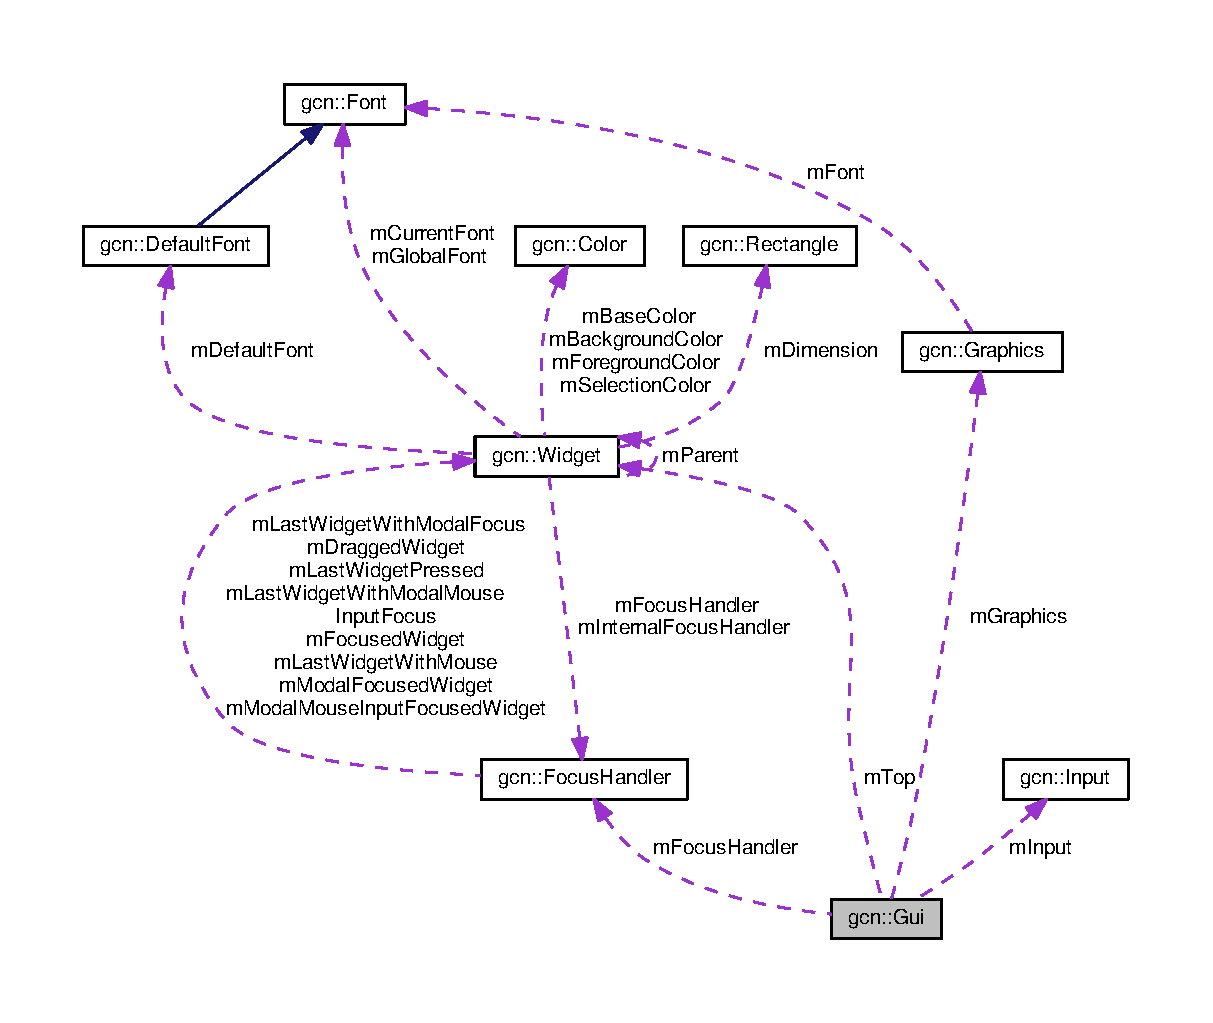
\includegraphics[width=350pt]{classgcn_1_1Gui__coll__graph}
\end{center}
\end{figure}
\subsection*{Public Member Functions}
\begin{DoxyCompactItemize}
\item 
\hyperlink{classgcn_1_1Gui_ada0ae56b26099a1bbb70fc4bb8d77da1}{Gui} ()
\item 
virtual \hyperlink{classgcn_1_1Gui_a89c4b4fafd6bc85646f90f6d03826d48}{$\sim$\+Gui} ()
\item 
virtual void \hyperlink{classgcn_1_1Gui_a69ce39ec8962ae93f428a01ffec677de}{set\+Top} (\hyperlink{classgcn_1_1Widget}{Widget} $\ast$top)
\item 
virtual \hyperlink{classgcn_1_1Widget}{Widget} $\ast$ \hyperlink{classgcn_1_1Gui_a020f9c4e1f533797c294630725561377}{get\+Top} () const 
\item 
virtual void \hyperlink{classgcn_1_1Gui_af8583f7e03da6cfe63794d05e185e1c0}{set\+Graphics} (\hyperlink{classgcn_1_1Graphics}{Graphics} $\ast$graphics)
\item 
virtual \hyperlink{classgcn_1_1Graphics}{Graphics} $\ast$ \hyperlink{classgcn_1_1Gui_a1f17a7727de5c35dc19bc1452cf37017}{get\+Graphics} () const 
\item 
virtual void \hyperlink{classgcn_1_1Gui_a317e8327dc9aee497f2a9ce1033d16c7}{set\+Input} (\hyperlink{classgcn_1_1Input}{Input} $\ast$input)
\item 
virtual \hyperlink{classgcn_1_1Input}{Input} $\ast$ \hyperlink{classgcn_1_1Gui_a9382a845e764178c741264e1a3acf837}{get\+Input} () const 
\item 
virtual void \hyperlink{classgcn_1_1Gui_a66744ebd628213d574bb6a7010781b1f}{logic} ()
\item 
virtual void \hyperlink{classgcn_1_1Gui_ad231f982fb8182b16ecf11075054f4ac}{draw} ()
\item 
virtual void \hyperlink{classgcn_1_1Gui_a273aa54779ea4d7b2f58e4a6b5907f48}{focus\+None} ()
\item 
virtual void \hyperlink{classgcn_1_1Gui_a5d2546bd8c6dbe288640163b85e94194}{set\+Tabbing\+Enabled} (bool tabbing)
\item 
virtual bool \hyperlink{classgcn_1_1Gui_aa77a86f825e8d03ea461e58a449b0179}{is\+Tabbing\+Enabled} ()
\item 
virtual void \hyperlink{classgcn_1_1Gui_a871191dc235cf6dd81aa8151eccd21a6}{add\+Global\+Key\+Listener} (\hyperlink{classgcn_1_1KeyListener}{Key\+Listener} $\ast$key\+Listener)
\item 
virtual void \hyperlink{classgcn_1_1Gui_a34a9488faca688e56b25df4a7297f4ea}{remove\+Global\+Key\+Listener} (\hyperlink{classgcn_1_1KeyListener}{Key\+Listener} $\ast$key\+Listener)
\end{DoxyCompactItemize}
\subsection*{Protected Types}
\begin{DoxyCompactItemize}
\item 
typedef std\+::list$<$ \hyperlink{classgcn_1_1KeyListener}{Key\+Listener} $\ast$ $>$ {\bfseries Key\+Listener\+List}\hypertarget{classgcn_1_1Gui_a1005100d790e06dafa0a8d338a14f289}{}\label{classgcn_1_1Gui_a1005100d790e06dafa0a8d338a14f289}

\item 
typedef Key\+Listener\+List\+::iterator {\bfseries Key\+Listener\+List\+Iterator}\hypertarget{classgcn_1_1Gui_a0a34fd3c5461fed924e22ccf36508a77}{}\label{classgcn_1_1Gui_a0a34fd3c5461fed924e22ccf36508a77}

\end{DoxyCompactItemize}
\subsection*{Protected Member Functions}
\begin{DoxyCompactItemize}
\item 
virtual void \hyperlink{classgcn_1_1Gui_a1208b3a8e98f54890864e020db204d82}{handle\+Mouse\+Input} ()
\item 
virtual void \hyperlink{classgcn_1_1Gui_a9ccdd4c90d5909c6a79d9e421aef0772}{handle\+Key\+Input} ()
\item 
virtual void \hyperlink{classgcn_1_1Gui_adc19660c008400343a35c47307861192}{handle\+Mouse\+Moved} (const \hyperlink{classgcn_1_1MouseInput}{Mouse\+Input} \&mouse\+Input)
\item 
virtual void \hyperlink{classgcn_1_1Gui_a24cf9a608ac21b734ef5e9d5a3a36b31}{handle\+Mouse\+Pressed} (const \hyperlink{classgcn_1_1MouseInput}{Mouse\+Input} \&mouse\+Input)
\item 
virtual void \hyperlink{classgcn_1_1Gui_ac0d9aa81a137206e6d73604994523842}{handle\+Mouse\+Wheel\+Moved\+Down} (const \hyperlink{classgcn_1_1MouseInput}{Mouse\+Input} \&mouse\+Input)
\item 
virtual void \hyperlink{classgcn_1_1Gui_a949c5513a73f39f94efecb84cd4d02d6}{handle\+Mouse\+Wheel\+Moved\+Up} (const \hyperlink{classgcn_1_1MouseInput}{Mouse\+Input} \&mouse\+Input)
\item 
virtual void \hyperlink{classgcn_1_1Gui_a2516448db507647152d97d8b600d2203}{handle\+Mouse\+Released} (const \hyperlink{classgcn_1_1MouseInput}{Mouse\+Input} \&mouse\+Input)
\item 
virtual void \hyperlink{classgcn_1_1Gui_a762a5583087900e1414091d3a3f3f18b}{handle\+Modal\+Focus} ()
\item 
virtual void \hyperlink{classgcn_1_1Gui_a9f85d69ebed46ca9d8441ac93cbbc1ec}{handle\+Modal\+Mouse\+Input\+Focus} ()
\item 
virtual void \hyperlink{classgcn_1_1Gui_a89afef358be49be921161f7c9d818976}{handle\+Modal\+Focus\+Gained} ()
\item 
virtual void \hyperlink{classgcn_1_1Gui_a4841624147d75ceccd080e2c98a3ff3e}{handle\+Modal\+Focus\+Released} ()
\item 
virtual void \hyperlink{classgcn_1_1Gui_a5aca2b2c0e168d5be705578b41bb2989}{distribute\+Mouse\+Event} (\hyperlink{classgcn_1_1Widget}{Widget} $\ast$source, int type, int button, int x, int y, bool force=false, bool to\+Source\+Only=false)
\item 
virtual void \hyperlink{classgcn_1_1Gui_aabaf700c710b66b93185c7733d820b07}{distribute\+Key\+Event} (\hyperlink{classgcn_1_1KeyEvent}{Key\+Event} \&key\+Event)
\item 
virtual void \hyperlink{classgcn_1_1Gui_a815207b12b22f2154cb8873f74f00d40}{distribute\+Key\+Event\+To\+Global\+Key\+Listeners} (\hyperlink{classgcn_1_1KeyEvent}{Key\+Event} \&key\+Event)
\item 
virtual \hyperlink{classgcn_1_1Widget}{Widget} $\ast$ \hyperlink{classgcn_1_1Gui_adbe10b9a50543f7f0ecaed5eb162c3c4}{get\+Widget\+At} (int x, int y)
\item 
virtual \hyperlink{classgcn_1_1Widget}{Widget} $\ast$ \hyperlink{classgcn_1_1Gui_a5e018eff39f41e7e7a9e52e3dd8a919e}{get\+Mouse\+Event\+Source} (int x, int y)
\item 
virtual \hyperlink{classgcn_1_1Widget}{Widget} $\ast$ \hyperlink{classgcn_1_1Gui_ad2e0e4f5cdfb5bc0901fdf81d222196f}{get\+Key\+Event\+Source} ()
\end{DoxyCompactItemize}
\subsection*{Protected Attributes}
\begin{DoxyCompactItemize}
\item 
\hyperlink{classgcn_1_1Widget}{Widget} $\ast$ {\bfseries m\+Top}\hypertarget{classgcn_1_1Gui_a604a47aac29b2b2d102fb9adf33046dd}{}\label{classgcn_1_1Gui_a604a47aac29b2b2d102fb9adf33046dd}

\item 
\hyperlink{classgcn_1_1Graphics}{Graphics} $\ast$ {\bfseries m\+Graphics}\hypertarget{classgcn_1_1Gui_abf24a26828a0714cb5b35874f1aeb2aa}{}\label{classgcn_1_1Gui_abf24a26828a0714cb5b35874f1aeb2aa}

\item 
\hyperlink{classgcn_1_1Input}{Input} $\ast$ {\bfseries m\+Input}\hypertarget{classgcn_1_1Gui_a3a5628dce778c217e817b40e552c1dd4}{}\label{classgcn_1_1Gui_a3a5628dce778c217e817b40e552c1dd4}

\item 
\hyperlink{classgcn_1_1FocusHandler}{Focus\+Handler} $\ast$ {\bfseries m\+Focus\+Handler}\hypertarget{classgcn_1_1Gui_a6d52184d92b5fb94c9e431310e822bb9}{}\label{classgcn_1_1Gui_a6d52184d92b5fb94c9e431310e822bb9}

\item 
bool {\bfseries m\+Tabbing}\hypertarget{classgcn_1_1Gui_a1cb20f54584e46d504fabaeca4937991}{}\label{classgcn_1_1Gui_a1cb20f54584e46d504fabaeca4937991}

\item 
Key\+Listener\+List {\bfseries m\+Key\+Listeners}\hypertarget{classgcn_1_1Gui_ad8ab94f193d8a00eebc9c562e723a94c}{}\label{classgcn_1_1Gui_ad8ab94f193d8a00eebc9c562e723a94c}

\item 
bool {\bfseries m\+Shift\+Pressed}\hypertarget{classgcn_1_1Gui_a5b45556c2b53be0f21adb7e8374d9ca9}{}\label{classgcn_1_1Gui_a5b45556c2b53be0f21adb7e8374d9ca9}

\item 
bool {\bfseries m\+Meta\+Pressed}\hypertarget{classgcn_1_1Gui_af12c89543b16cffb8c2d3696058ea105}{}\label{classgcn_1_1Gui_af12c89543b16cffb8c2d3696058ea105}

\item 
bool {\bfseries m\+Control\+Pressed}\hypertarget{classgcn_1_1Gui_afc00084e5947095924a868c2a3e39c39}{}\label{classgcn_1_1Gui_afc00084e5947095924a868c2a3e39c39}

\item 
bool {\bfseries m\+Alt\+Pressed}\hypertarget{classgcn_1_1Gui_a678962cf7e90a820660e37e36a020881}{}\label{classgcn_1_1Gui_a678962cf7e90a820660e37e36a020881}

\item 
unsigned int {\bfseries m\+Last\+Mouse\+Press\+Button}\hypertarget{classgcn_1_1Gui_ac2b85afc91a28d5e9b3b88c685b4e102}{}\label{classgcn_1_1Gui_ac2b85afc91a28d5e9b3b88c685b4e102}

\item 
int {\bfseries m\+Last\+Mouse\+Press\+Time\+Stamp}\hypertarget{classgcn_1_1Gui_acde4e38a2c4c1078ff88920b93167fb0}{}\label{classgcn_1_1Gui_acde4e38a2c4c1078ff88920b93167fb0}

\item 
int {\bfseries m\+Last\+MouseX}\hypertarget{classgcn_1_1Gui_a06bbfa9a446a238918ea21018e3b17a2}{}\label{classgcn_1_1Gui_a06bbfa9a446a238918ea21018e3b17a2}

\item 
int {\bfseries m\+Last\+MouseY}\hypertarget{classgcn_1_1Gui_a68df34ed2f71cdcff2b80f8deca645d4}{}\label{classgcn_1_1Gui_a68df34ed2f71cdcff2b80f8deca645d4}

\item 
int {\bfseries m\+Click\+Count}\hypertarget{classgcn_1_1Gui_ab08a032e0ec6b8cabed5dae39f5be9ce}{}\label{classgcn_1_1Gui_ab08a032e0ec6b8cabed5dae39f5be9ce}

\item 
int {\bfseries m\+Last\+Mouse\+Drag\+Button}\hypertarget{classgcn_1_1Gui_a2277fca30ae196ee34b231724454d268}{}\label{classgcn_1_1Gui_a2277fca30ae196ee34b231724454d268}

\item 
std\+::deque$<$ \hyperlink{classgcn_1_1Widget}{Widget} $\ast$ $>$ {\bfseries m\+Widget\+With\+Mouse\+Queue}\hypertarget{classgcn_1_1Gui_a0a6fc16b8724b80350742f05bf79aff1}{}\label{classgcn_1_1Gui_a0a6fc16b8724b80350742f05bf79aff1}

\end{DoxyCompactItemize}


\subsection{Detailed Description}
\hyperlink{classgcn_1_1Gui}{Gui} core class. Contains a special widget called the top widget. If you want to be able to have more then one \hyperlink{classgcn_1_1Widget}{Widget} in your \hyperlink{classgcn_1_1Gui}{Gui}, the top widget should be a \hyperlink{classgcn_1_1Container}{Container}.

N\+O\+TE\+: For the \hyperlink{classgcn_1_1Gui}{Gui} to function properly you need to set a \hyperlink{classgcn_1_1Graphics}{Graphics} object to use and an \hyperlink{classgcn_1_1Input}{Input} object to use. 

\subsection{Constructor \& Destructor Documentation}
\index{gcn\+::\+Gui@{gcn\+::\+Gui}!Gui@{Gui}}
\index{Gui@{Gui}!gcn\+::\+Gui@{gcn\+::\+Gui}}
\subsubsection[{\texorpdfstring{Gui()}{Gui()}}]{\setlength{\rightskip}{0pt plus 5cm}gcn\+::\+Gui\+::\+Gui (
\begin{DoxyParamCaption}
{}
\end{DoxyParamCaption}
)}\hypertarget{classgcn_1_1Gui_ada0ae56b26099a1bbb70fc4bb8d77da1}{}\label{classgcn_1_1Gui_ada0ae56b26099a1bbb70fc4bb8d77da1}
Constructor. \index{gcn\+::\+Gui@{gcn\+::\+Gui}!````~Gui@{$\sim$\+Gui}}
\index{````~Gui@{$\sim$\+Gui}!gcn\+::\+Gui@{gcn\+::\+Gui}}
\subsubsection[{\texorpdfstring{$\sim$\+Gui()}{~Gui()}}]{\setlength{\rightskip}{0pt plus 5cm}gcn\+::\+Gui\+::$\sim$\+Gui (
\begin{DoxyParamCaption}
{}
\end{DoxyParamCaption}
)\hspace{0.3cm}{\ttfamily [virtual]}}\hypertarget{classgcn_1_1Gui_a89c4b4fafd6bc85646f90f6d03826d48}{}\label{classgcn_1_1Gui_a89c4b4fafd6bc85646f90f6d03826d48}
Destructor. 

\subsection{Member Function Documentation}
\index{gcn\+::\+Gui@{gcn\+::\+Gui}!add\+Global\+Key\+Listener@{add\+Global\+Key\+Listener}}
\index{add\+Global\+Key\+Listener@{add\+Global\+Key\+Listener}!gcn\+::\+Gui@{gcn\+::\+Gui}}
\subsubsection[{\texorpdfstring{add\+Global\+Key\+Listener(\+Key\+Listener $\ast$key\+Listener)}{addGlobalKeyListener(KeyListener *keyListener)}}]{\setlength{\rightskip}{0pt plus 5cm}void gcn\+::\+Gui\+::add\+Global\+Key\+Listener (
\begin{DoxyParamCaption}
\item[{{\bf Key\+Listener} $\ast$}]{key\+Listener}
\end{DoxyParamCaption}
)\hspace{0.3cm}{\ttfamily [virtual]}}\hypertarget{classgcn_1_1Gui_a871191dc235cf6dd81aa8151eccd21a6}{}\label{classgcn_1_1Gui_a871191dc235cf6dd81aa8151eccd21a6}
Adds a global \hyperlink{classgcn_1_1KeyListener}{Key\+Listener} to the \hyperlink{classgcn_1_1Gui}{Gui}.


\begin{DoxyParams}{Parameters}
{\em key\+Listener} & a \hyperlink{classgcn_1_1KeyListener}{Key\+Listener} to add. \\
\hline
\end{DoxyParams}
\index{gcn\+::\+Gui@{gcn\+::\+Gui}!distribute\+Key\+Event@{distribute\+Key\+Event}}
\index{distribute\+Key\+Event@{distribute\+Key\+Event}!gcn\+::\+Gui@{gcn\+::\+Gui}}
\subsubsection[{\texorpdfstring{distribute\+Key\+Event(\+Key\+Event \&key\+Event)}{distributeKeyEvent(KeyEvent &keyEvent)}}]{\setlength{\rightskip}{0pt plus 5cm}void gcn\+::\+Gui\+::distribute\+Key\+Event (
\begin{DoxyParamCaption}
\item[{{\bf Key\+Event} \&}]{key\+Event}
\end{DoxyParamCaption}
)\hspace{0.3cm}{\ttfamily [protected]}, {\ttfamily [virtual]}}\hypertarget{classgcn_1_1Gui_aabaf700c710b66b93185c7733d820b07}{}\label{classgcn_1_1Gui_aabaf700c710b66b93185c7733d820b07}
Distributes a key event.


\begin{DoxyParams}{Parameters}
{\em key\+Event} & the key event to distribute.\\
\hline
\end{DoxyParams}
\begin{DoxySince}{Since}
0.\+6.\+0 
\end{DoxySince}
\index{gcn\+::\+Gui@{gcn\+::\+Gui}!distribute\+Key\+Event\+To\+Global\+Key\+Listeners@{distribute\+Key\+Event\+To\+Global\+Key\+Listeners}}
\index{distribute\+Key\+Event\+To\+Global\+Key\+Listeners@{distribute\+Key\+Event\+To\+Global\+Key\+Listeners}!gcn\+::\+Gui@{gcn\+::\+Gui}}
\subsubsection[{\texorpdfstring{distribute\+Key\+Event\+To\+Global\+Key\+Listeners(\+Key\+Event \&key\+Event)}{distributeKeyEventToGlobalKeyListeners(KeyEvent &keyEvent)}}]{\setlength{\rightskip}{0pt plus 5cm}void gcn\+::\+Gui\+::distribute\+Key\+Event\+To\+Global\+Key\+Listeners (
\begin{DoxyParamCaption}
\item[{{\bf Key\+Event} \&}]{key\+Event}
\end{DoxyParamCaption}
)\hspace{0.3cm}{\ttfamily [protected]}, {\ttfamily [virtual]}}\hypertarget{classgcn_1_1Gui_a815207b12b22f2154cb8873f74f00d40}{}\label{classgcn_1_1Gui_a815207b12b22f2154cb8873f74f00d40}
Distributes a key event to the global key listeners.


\begin{DoxyParams}{Parameters}
{\em key\+Event} & the key event to distribute.\\
\hline
\end{DoxyParams}
\begin{DoxySince}{Since}
0.\+6.\+0 
\end{DoxySince}
\index{gcn\+::\+Gui@{gcn\+::\+Gui}!distribute\+Mouse\+Event@{distribute\+Mouse\+Event}}
\index{distribute\+Mouse\+Event@{distribute\+Mouse\+Event}!gcn\+::\+Gui@{gcn\+::\+Gui}}
\subsubsection[{\texorpdfstring{distribute\+Mouse\+Event(\+Widget $\ast$source, int type, int button, int x, int y, bool force=false, bool to\+Source\+Only=false)}{distributeMouseEvent(Widget *source, int type, int button, int x, int y, bool force=false, bool toSourceOnly=false)}}]{\setlength{\rightskip}{0pt plus 5cm}void gcn\+::\+Gui\+::distribute\+Mouse\+Event (
\begin{DoxyParamCaption}
\item[{{\bf Widget} $\ast$}]{source, }
\item[{int}]{type, }
\item[{int}]{button, }
\item[{int}]{x, }
\item[{int}]{y, }
\item[{bool}]{force = {\ttfamily false}, }
\item[{bool}]{to\+Source\+Only = {\ttfamily false}}
\end{DoxyParamCaption}
)\hspace{0.3cm}{\ttfamily [protected]}, {\ttfamily [virtual]}}\hypertarget{classgcn_1_1Gui_a5aca2b2c0e168d5be705578b41bb2989}{}\label{classgcn_1_1Gui_a5aca2b2c0e168d5be705578b41bb2989}
Distributes a mouse event.


\begin{DoxyParams}{Parameters}
{\em type} & The type of the event to distribute, \\
\hline
{\em button} & The button of the event (if any used) to distribute. \\
\hline
{\em x} & The x coordinate of the event. \\
\hline
{\em y} & The y coordinate of the event. \\
\hline
{\em fource} & indicates whether the distribution should be forced or not. A forced distribution distributes the event even if a widget is not enabled, not visible, another widget has modal focus or another widget has modal mouse input focus. Default value is false. \\
\hline
{\em to\+Source\+Only} & indicates whether the distribution should be to the source widget only or to it\textquotesingle{}s parent\textquotesingle{}s mouse listeners as well.\\
\hline
\end{DoxyParams}
\begin{DoxySince}{Since}
0.\+6.\+0 
\end{DoxySince}
\index{gcn\+::\+Gui@{gcn\+::\+Gui}!draw@{draw}}
\index{draw@{draw}!gcn\+::\+Gui@{gcn\+::\+Gui}}
\subsubsection[{\texorpdfstring{draw()}{draw()}}]{\setlength{\rightskip}{0pt plus 5cm}void gcn\+::\+Gui\+::draw (
\begin{DoxyParamCaption}
{}
\end{DoxyParamCaption}
)\hspace{0.3cm}{\ttfamily [virtual]}}\hypertarget{classgcn_1_1Gui_ad231f982fb8182b16ecf11075054f4ac}{}\label{classgcn_1_1Gui_ad231f982fb8182b16ecf11075054f4ac}
Draws the \hyperlink{classgcn_1_1Gui}{Gui}. By calling this funcion all draw functions down in the \hyperlink{classgcn_1_1Gui}{Gui} hierarchy will be called. \index{gcn\+::\+Gui@{gcn\+::\+Gui}!focus\+None@{focus\+None}}
\index{focus\+None@{focus\+None}!gcn\+::\+Gui@{gcn\+::\+Gui}}
\subsubsection[{\texorpdfstring{focus\+None()}{focusNone()}}]{\setlength{\rightskip}{0pt plus 5cm}void gcn\+::\+Gui\+::focus\+None (
\begin{DoxyParamCaption}
{}
\end{DoxyParamCaption}
)\hspace{0.3cm}{\ttfamily [virtual]}}\hypertarget{classgcn_1_1Gui_a273aa54779ea4d7b2f58e4a6b5907f48}{}\label{classgcn_1_1Gui_a273aa54779ea4d7b2f58e4a6b5907f48}
Focus none of the Widgets in the \hyperlink{classgcn_1_1Gui}{Gui}. \index{gcn\+::\+Gui@{gcn\+::\+Gui}!get\+Graphics@{get\+Graphics}}
\index{get\+Graphics@{get\+Graphics}!gcn\+::\+Gui@{gcn\+::\+Gui}}
\subsubsection[{\texorpdfstring{get\+Graphics() const }{getGraphics() const }}]{\setlength{\rightskip}{0pt plus 5cm}{\bf Graphics} $\ast$ gcn\+::\+Gui\+::get\+Graphics (
\begin{DoxyParamCaption}
{}
\end{DoxyParamCaption}
) const\hspace{0.3cm}{\ttfamily [virtual]}}\hypertarget{classgcn_1_1Gui_a1f17a7727de5c35dc19bc1452cf37017}{}\label{classgcn_1_1Gui_a1f17a7727de5c35dc19bc1452cf37017}
Gets the \hyperlink{classgcn_1_1Graphics}{Graphics} object used for drawing.

\begin{DoxyReturn}{Returns}
the \hyperlink{classgcn_1_1Graphics}{Graphics} object used for drawing. N\+U\+LL if no \hyperlink{classgcn_1_1Graphics}{Graphics} object has been set. 
\end{DoxyReturn}
\index{gcn\+::\+Gui@{gcn\+::\+Gui}!get\+Input@{get\+Input}}
\index{get\+Input@{get\+Input}!gcn\+::\+Gui@{gcn\+::\+Gui}}
\subsubsection[{\texorpdfstring{get\+Input() const }{getInput() const }}]{\setlength{\rightskip}{0pt plus 5cm}{\bf Input} $\ast$ gcn\+::\+Gui\+::get\+Input (
\begin{DoxyParamCaption}
{}
\end{DoxyParamCaption}
) const\hspace{0.3cm}{\ttfamily [virtual]}}\hypertarget{classgcn_1_1Gui_a9382a845e764178c741264e1a3acf837}{}\label{classgcn_1_1Gui_a9382a845e764178c741264e1a3acf837}
Gets the \hyperlink{classgcn_1_1Input}{Input} object being used for input handling.

\begin{DoxyReturn}{Returns}
the \hyperlink{classgcn_1_1Input}{Input} object used for handling input. N\+U\+LL if no \hyperlink{classgcn_1_1Input}{Input} object has been set. 
\end{DoxyReturn}
\index{gcn\+::\+Gui@{gcn\+::\+Gui}!get\+Key\+Event\+Source@{get\+Key\+Event\+Source}}
\index{get\+Key\+Event\+Source@{get\+Key\+Event\+Source}!gcn\+::\+Gui@{gcn\+::\+Gui}}
\subsubsection[{\texorpdfstring{get\+Key\+Event\+Source()}{getKeyEventSource()}}]{\setlength{\rightskip}{0pt plus 5cm}{\bf Widget} $\ast$ gcn\+::\+Gui\+::get\+Key\+Event\+Source (
\begin{DoxyParamCaption}
{}
\end{DoxyParamCaption}
)\hspace{0.3cm}{\ttfamily [protected]}, {\ttfamily [virtual]}}\hypertarget{classgcn_1_1Gui_ad2e0e4f5cdfb5bc0901fdf81d222196f}{}\label{classgcn_1_1Gui_ad2e0e4f5cdfb5bc0901fdf81d222196f}
Gets the source of the key event.

\begin{DoxyReturn}{Returns}
the source widget of the key event. 
\end{DoxyReturn}
\begin{DoxySince}{Since}
0.\+6.\+0 
\end{DoxySince}
\index{gcn\+::\+Gui@{gcn\+::\+Gui}!get\+Mouse\+Event\+Source@{get\+Mouse\+Event\+Source}}
\index{get\+Mouse\+Event\+Source@{get\+Mouse\+Event\+Source}!gcn\+::\+Gui@{gcn\+::\+Gui}}
\subsubsection[{\texorpdfstring{get\+Mouse\+Event\+Source(int x, int y)}{getMouseEventSource(int x, int y)}}]{\setlength{\rightskip}{0pt plus 5cm}{\bf Widget} $\ast$ gcn\+::\+Gui\+::get\+Mouse\+Event\+Source (
\begin{DoxyParamCaption}
\item[{int}]{x, }
\item[{int}]{y}
\end{DoxyParamCaption}
)\hspace{0.3cm}{\ttfamily [protected]}, {\ttfamily [virtual]}}\hypertarget{classgcn_1_1Gui_a5e018eff39f41e7e7a9e52e3dd8a919e}{}\label{classgcn_1_1Gui_a5e018eff39f41e7e7a9e52e3dd8a919e}
Gets the source of the mouse event.

\begin{DoxyReturn}{Returns}
the source widget of the mouse event. 
\end{DoxyReturn}
\begin{DoxySince}{Since}
0.\+6.\+0 
\end{DoxySince}
\index{gcn\+::\+Gui@{gcn\+::\+Gui}!get\+Top@{get\+Top}}
\index{get\+Top@{get\+Top}!gcn\+::\+Gui@{gcn\+::\+Gui}}
\subsubsection[{\texorpdfstring{get\+Top() const }{getTop() const }}]{\setlength{\rightskip}{0pt plus 5cm}{\bf Widget} $\ast$ gcn\+::\+Gui\+::get\+Top (
\begin{DoxyParamCaption}
{}
\end{DoxyParamCaption}
) const\hspace{0.3cm}{\ttfamily [virtual]}}\hypertarget{classgcn_1_1Gui_a020f9c4e1f533797c294630725561377}{}\label{classgcn_1_1Gui_a020f9c4e1f533797c294630725561377}
Gets the top \hyperlink{classgcn_1_1Widget}{Widget}.

\begin{DoxyReturn}{Returns}
the top widget. N\+U\+LL if no top widget has been set. 
\end{DoxyReturn}
\index{gcn\+::\+Gui@{gcn\+::\+Gui}!get\+Widget\+At@{get\+Widget\+At}}
\index{get\+Widget\+At@{get\+Widget\+At}!gcn\+::\+Gui@{gcn\+::\+Gui}}
\subsubsection[{\texorpdfstring{get\+Widget\+At(int x, int y)}{getWidgetAt(int x, int y)}}]{\setlength{\rightskip}{0pt plus 5cm}{\bf Widget} $\ast$ gcn\+::\+Gui\+::get\+Widget\+At (
\begin{DoxyParamCaption}
\item[{int}]{x, }
\item[{int}]{y}
\end{DoxyParamCaption}
)\hspace{0.3cm}{\ttfamily [protected]}, {\ttfamily [virtual]}}\hypertarget{classgcn_1_1Gui_adbe10b9a50543f7f0ecaed5eb162c3c4}{}\label{classgcn_1_1Gui_adbe10b9a50543f7f0ecaed5eb162c3c4}
Gets the widget at a certain position.

\begin{DoxyReturn}{Returns}
the widget at a certain position. 
\end{DoxyReturn}
\begin{DoxySince}{Since}
0.\+6.\+0 
\end{DoxySince}
\index{gcn\+::\+Gui@{gcn\+::\+Gui}!handle\+Key\+Input@{handle\+Key\+Input}}
\index{handle\+Key\+Input@{handle\+Key\+Input}!gcn\+::\+Gui@{gcn\+::\+Gui}}
\subsubsection[{\texorpdfstring{handle\+Key\+Input()}{handleKeyInput()}}]{\setlength{\rightskip}{0pt plus 5cm}void gcn\+::\+Gui\+::handle\+Key\+Input (
\begin{DoxyParamCaption}
{}
\end{DoxyParamCaption}
)\hspace{0.3cm}{\ttfamily [protected]}, {\ttfamily [virtual]}}\hypertarget{classgcn_1_1Gui_a9ccdd4c90d5909c6a79d9e421aef0772}{}\label{classgcn_1_1Gui_a9ccdd4c90d5909c6a79d9e421aef0772}
Handles key input.

\begin{DoxySince}{Since}
0.\+6.\+0 
\end{DoxySince}
\index{gcn\+::\+Gui@{gcn\+::\+Gui}!handle\+Modal\+Focus@{handle\+Modal\+Focus}}
\index{handle\+Modal\+Focus@{handle\+Modal\+Focus}!gcn\+::\+Gui@{gcn\+::\+Gui}}
\subsubsection[{\texorpdfstring{handle\+Modal\+Focus()}{handleModalFocus()}}]{\setlength{\rightskip}{0pt plus 5cm}void gcn\+::\+Gui\+::handle\+Modal\+Focus (
\begin{DoxyParamCaption}
{}
\end{DoxyParamCaption}
)\hspace{0.3cm}{\ttfamily [protected]}, {\ttfamily [virtual]}}\hypertarget{classgcn_1_1Gui_a762a5583087900e1414091d3a3f3f18b}{}\label{classgcn_1_1Gui_a762a5583087900e1414091d3a3f3f18b}
Handles modal focus. Modal focus needs to be checked at each logic iteration as it might be necessary to distribute mouse entered or mouse exited events.

\begin{DoxySince}{Since}
0.\+8.\+0 
\end{DoxySince}
\index{gcn\+::\+Gui@{gcn\+::\+Gui}!handle\+Modal\+Focus\+Gained@{handle\+Modal\+Focus\+Gained}}
\index{handle\+Modal\+Focus\+Gained@{handle\+Modal\+Focus\+Gained}!gcn\+::\+Gui@{gcn\+::\+Gui}}
\subsubsection[{\texorpdfstring{handle\+Modal\+Focus\+Gained()}{handleModalFocusGained()}}]{\setlength{\rightskip}{0pt plus 5cm}void gcn\+::\+Gui\+::handle\+Modal\+Focus\+Gained (
\begin{DoxyParamCaption}
{}
\end{DoxyParamCaption}
)\hspace{0.3cm}{\ttfamily [protected]}, {\ttfamily [virtual]}}\hypertarget{classgcn_1_1Gui_a89afef358be49be921161f7c9d818976}{}\label{classgcn_1_1Gui_a89afef358be49be921161f7c9d818976}
Handles modal focus gained. If modal focus has been gaind it might be necessary to distribute mouse entered or mouse exited events.

\begin{DoxySince}{Since}
0.\+8.\+0 
\end{DoxySince}
\index{gcn\+::\+Gui@{gcn\+::\+Gui}!handle\+Modal\+Focus\+Released@{handle\+Modal\+Focus\+Released}}
\index{handle\+Modal\+Focus\+Released@{handle\+Modal\+Focus\+Released}!gcn\+::\+Gui@{gcn\+::\+Gui}}
\subsubsection[{\texorpdfstring{handle\+Modal\+Focus\+Released()}{handleModalFocusReleased()}}]{\setlength{\rightskip}{0pt plus 5cm}void gcn\+::\+Gui\+::handle\+Modal\+Focus\+Released (
\begin{DoxyParamCaption}
{}
\end{DoxyParamCaption}
)\hspace{0.3cm}{\ttfamily [protected]}, {\ttfamily [virtual]}}\hypertarget{classgcn_1_1Gui_a4841624147d75ceccd080e2c98a3ff3e}{}\label{classgcn_1_1Gui_a4841624147d75ceccd080e2c98a3ff3e}
Handles modal mouse input focus gained. If modal focus has been gaind it might be necessary to distribute mouse entered or mouse exited events.

\begin{DoxySince}{Since}
0.\+8.\+0 
\end{DoxySince}
\index{gcn\+::\+Gui@{gcn\+::\+Gui}!handle\+Modal\+Mouse\+Input\+Focus@{handle\+Modal\+Mouse\+Input\+Focus}}
\index{handle\+Modal\+Mouse\+Input\+Focus@{handle\+Modal\+Mouse\+Input\+Focus}!gcn\+::\+Gui@{gcn\+::\+Gui}}
\subsubsection[{\texorpdfstring{handle\+Modal\+Mouse\+Input\+Focus()}{handleModalMouseInputFocus()}}]{\setlength{\rightskip}{0pt plus 5cm}void gcn\+::\+Gui\+::handle\+Modal\+Mouse\+Input\+Focus (
\begin{DoxyParamCaption}
{}
\end{DoxyParamCaption}
)\hspace{0.3cm}{\ttfamily [protected]}, {\ttfamily [virtual]}}\hypertarget{classgcn_1_1Gui_a9f85d69ebed46ca9d8441ac93cbbc1ec}{}\label{classgcn_1_1Gui_a9f85d69ebed46ca9d8441ac93cbbc1ec}
Handles modal mouse input focus. Modal mouse input focus needs to be checked at each logic iteration as it might be necessary to distribute mouse entered or mouse exited events.

\begin{DoxySince}{Since}
0.\+8.\+0 
\end{DoxySince}
\index{gcn\+::\+Gui@{gcn\+::\+Gui}!handle\+Mouse\+Input@{handle\+Mouse\+Input}}
\index{handle\+Mouse\+Input@{handle\+Mouse\+Input}!gcn\+::\+Gui@{gcn\+::\+Gui}}
\subsubsection[{\texorpdfstring{handle\+Mouse\+Input()}{handleMouseInput()}}]{\setlength{\rightskip}{0pt plus 5cm}void gcn\+::\+Gui\+::handle\+Mouse\+Input (
\begin{DoxyParamCaption}
{}
\end{DoxyParamCaption}
)\hspace{0.3cm}{\ttfamily [protected]}, {\ttfamily [virtual]}}\hypertarget{classgcn_1_1Gui_a1208b3a8e98f54890864e020db204d82}{}\label{classgcn_1_1Gui_a1208b3a8e98f54890864e020db204d82}
Handles all mouse input.

\begin{DoxySince}{Since}
0.\+6.\+0 
\end{DoxySince}
\index{gcn\+::\+Gui@{gcn\+::\+Gui}!handle\+Mouse\+Moved@{handle\+Mouse\+Moved}}
\index{handle\+Mouse\+Moved@{handle\+Mouse\+Moved}!gcn\+::\+Gui@{gcn\+::\+Gui}}
\subsubsection[{\texorpdfstring{handle\+Mouse\+Moved(const Mouse\+Input \&mouse\+Input)}{handleMouseMoved(const MouseInput &mouseInput)}}]{\setlength{\rightskip}{0pt plus 5cm}void gcn\+::\+Gui\+::handle\+Mouse\+Moved (
\begin{DoxyParamCaption}
\item[{const {\bf Mouse\+Input} \&}]{mouse\+Input}
\end{DoxyParamCaption}
)\hspace{0.3cm}{\ttfamily [protected]}, {\ttfamily [virtual]}}\hypertarget{classgcn_1_1Gui_adc19660c008400343a35c47307861192}{}\label{classgcn_1_1Gui_adc19660c008400343a35c47307861192}
Handles mouse moved input.


\begin{DoxyParams}{Parameters}
{\em mouse\+Input} & the mouse input to handle. \\
\hline
\end{DoxyParams}
\begin{DoxySince}{Since}
0.\+6.\+0 
\end{DoxySince}
\index{gcn\+::\+Gui@{gcn\+::\+Gui}!handle\+Mouse\+Pressed@{handle\+Mouse\+Pressed}}
\index{handle\+Mouse\+Pressed@{handle\+Mouse\+Pressed}!gcn\+::\+Gui@{gcn\+::\+Gui}}
\subsubsection[{\texorpdfstring{handle\+Mouse\+Pressed(const Mouse\+Input \&mouse\+Input)}{handleMousePressed(const MouseInput &mouseInput)}}]{\setlength{\rightskip}{0pt plus 5cm}void gcn\+::\+Gui\+::handle\+Mouse\+Pressed (
\begin{DoxyParamCaption}
\item[{const {\bf Mouse\+Input} \&}]{mouse\+Input}
\end{DoxyParamCaption}
)\hspace{0.3cm}{\ttfamily [protected]}, {\ttfamily [virtual]}}\hypertarget{classgcn_1_1Gui_a24cf9a608ac21b734ef5e9d5a3a36b31}{}\label{classgcn_1_1Gui_a24cf9a608ac21b734ef5e9d5a3a36b31}
Handles mouse pressed input.


\begin{DoxyParams}{Parameters}
{\em mouse\+Input} & the mouse input to handle. \\
\hline
\end{DoxyParams}
\begin{DoxySince}{Since}
0.\+6.\+0 
\end{DoxySince}
\index{gcn\+::\+Gui@{gcn\+::\+Gui}!handle\+Mouse\+Released@{handle\+Mouse\+Released}}
\index{handle\+Mouse\+Released@{handle\+Mouse\+Released}!gcn\+::\+Gui@{gcn\+::\+Gui}}
\subsubsection[{\texorpdfstring{handle\+Mouse\+Released(const Mouse\+Input \&mouse\+Input)}{handleMouseReleased(const MouseInput &mouseInput)}}]{\setlength{\rightskip}{0pt plus 5cm}void gcn\+::\+Gui\+::handle\+Mouse\+Released (
\begin{DoxyParamCaption}
\item[{const {\bf Mouse\+Input} \&}]{mouse\+Input}
\end{DoxyParamCaption}
)\hspace{0.3cm}{\ttfamily [protected]}, {\ttfamily [virtual]}}\hypertarget{classgcn_1_1Gui_a2516448db507647152d97d8b600d2203}{}\label{classgcn_1_1Gui_a2516448db507647152d97d8b600d2203}
Handles mouse released input.


\begin{DoxyParams}{Parameters}
{\em mouse\+Input} & the mouse input to handle. \\
\hline
\end{DoxyParams}
\begin{DoxySince}{Since}
0.\+6.\+0 
\end{DoxySince}
\index{gcn\+::\+Gui@{gcn\+::\+Gui}!handle\+Mouse\+Wheel\+Moved\+Down@{handle\+Mouse\+Wheel\+Moved\+Down}}
\index{handle\+Mouse\+Wheel\+Moved\+Down@{handle\+Mouse\+Wheel\+Moved\+Down}!gcn\+::\+Gui@{gcn\+::\+Gui}}
\subsubsection[{\texorpdfstring{handle\+Mouse\+Wheel\+Moved\+Down(const Mouse\+Input \&mouse\+Input)}{handleMouseWheelMovedDown(const MouseInput &mouseInput)}}]{\setlength{\rightskip}{0pt plus 5cm}void gcn\+::\+Gui\+::handle\+Mouse\+Wheel\+Moved\+Down (
\begin{DoxyParamCaption}
\item[{const {\bf Mouse\+Input} \&}]{mouse\+Input}
\end{DoxyParamCaption}
)\hspace{0.3cm}{\ttfamily [protected]}, {\ttfamily [virtual]}}\hypertarget{classgcn_1_1Gui_ac0d9aa81a137206e6d73604994523842}{}\label{classgcn_1_1Gui_ac0d9aa81a137206e6d73604994523842}
Handles mouse wheel moved down input.


\begin{DoxyParams}{Parameters}
{\em mouse\+Input} & the mouse input to handle. \\
\hline
\end{DoxyParams}
\begin{DoxySince}{Since}
0.\+6.\+0 
\end{DoxySince}
\index{gcn\+::\+Gui@{gcn\+::\+Gui}!handle\+Mouse\+Wheel\+Moved\+Up@{handle\+Mouse\+Wheel\+Moved\+Up}}
\index{handle\+Mouse\+Wheel\+Moved\+Up@{handle\+Mouse\+Wheel\+Moved\+Up}!gcn\+::\+Gui@{gcn\+::\+Gui}}
\subsubsection[{\texorpdfstring{handle\+Mouse\+Wheel\+Moved\+Up(const Mouse\+Input \&mouse\+Input)}{handleMouseWheelMovedUp(const MouseInput &mouseInput)}}]{\setlength{\rightskip}{0pt plus 5cm}void gcn\+::\+Gui\+::handle\+Mouse\+Wheel\+Moved\+Up (
\begin{DoxyParamCaption}
\item[{const {\bf Mouse\+Input} \&}]{mouse\+Input}
\end{DoxyParamCaption}
)\hspace{0.3cm}{\ttfamily [protected]}, {\ttfamily [virtual]}}\hypertarget{classgcn_1_1Gui_a949c5513a73f39f94efecb84cd4d02d6}{}\label{classgcn_1_1Gui_a949c5513a73f39f94efecb84cd4d02d6}
Handles mouse wheel moved up input.


\begin{DoxyParams}{Parameters}
{\em mouse\+Input} & the mouse input to handle. \\
\hline
\end{DoxyParams}
\begin{DoxySince}{Since}
0.\+6.\+0 
\end{DoxySince}
\index{gcn\+::\+Gui@{gcn\+::\+Gui}!is\+Tabbing\+Enabled@{is\+Tabbing\+Enabled}}
\index{is\+Tabbing\+Enabled@{is\+Tabbing\+Enabled}!gcn\+::\+Gui@{gcn\+::\+Gui}}
\subsubsection[{\texorpdfstring{is\+Tabbing\+Enabled()}{isTabbingEnabled()}}]{\setlength{\rightskip}{0pt plus 5cm}bool gcn\+::\+Gui\+::is\+Tabbing\+Enabled (
\begin{DoxyParamCaption}
{}
\end{DoxyParamCaption}
)\hspace{0.3cm}{\ttfamily [virtual]}}\hypertarget{classgcn_1_1Gui_aa77a86f825e8d03ea461e58a449b0179}{}\label{classgcn_1_1Gui_aa77a86f825e8d03ea461e58a449b0179}
Checks if tabbing is enabled.

\begin{DoxyReturn}{Returns}
true if tabbing is enabled. 
\end{DoxyReturn}
\index{gcn\+::\+Gui@{gcn\+::\+Gui}!logic@{logic}}
\index{logic@{logic}!gcn\+::\+Gui@{gcn\+::\+Gui}}
\subsubsection[{\texorpdfstring{logic()}{logic()}}]{\setlength{\rightskip}{0pt plus 5cm}void gcn\+::\+Gui\+::logic (
\begin{DoxyParamCaption}
{}
\end{DoxyParamCaption}
)\hspace{0.3cm}{\ttfamily [virtual]}}\hypertarget{classgcn_1_1Gui_a66744ebd628213d574bb6a7010781b1f}{}\label{classgcn_1_1Gui_a66744ebd628213d574bb6a7010781b1f}
Performs the \hyperlink{classgcn_1_1Gui}{Gui} logic. By calling this function all logic functions down in the \hyperlink{classgcn_1_1Gui}{Gui} heirarchy will be called. What performs in Logic can be just about anything like adjusting a Widgets size or doing some calculations.

N\+O\+TE\+: Logic also deals with user input (Mouse and Keyboard) for Widgets. \index{gcn\+::\+Gui@{gcn\+::\+Gui}!remove\+Global\+Key\+Listener@{remove\+Global\+Key\+Listener}}
\index{remove\+Global\+Key\+Listener@{remove\+Global\+Key\+Listener}!gcn\+::\+Gui@{gcn\+::\+Gui}}
\subsubsection[{\texorpdfstring{remove\+Global\+Key\+Listener(\+Key\+Listener $\ast$key\+Listener)}{removeGlobalKeyListener(KeyListener *keyListener)}}]{\setlength{\rightskip}{0pt plus 5cm}void gcn\+::\+Gui\+::remove\+Global\+Key\+Listener (
\begin{DoxyParamCaption}
\item[{{\bf Key\+Listener} $\ast$}]{key\+Listener}
\end{DoxyParamCaption}
)\hspace{0.3cm}{\ttfamily [virtual]}}\hypertarget{classgcn_1_1Gui_a34a9488faca688e56b25df4a7297f4ea}{}\label{classgcn_1_1Gui_a34a9488faca688e56b25df4a7297f4ea}
Remove global \hyperlink{classgcn_1_1KeyListener}{Key\+Listener} from the \hyperlink{classgcn_1_1Gui}{Gui}.


\begin{DoxyParams}{Parameters}
{\em key\+Listener} & a \hyperlink{classgcn_1_1KeyListener}{Key\+Listener} to remove. \\
\hline
\end{DoxyParams}

\begin{DoxyExceptions}{Exceptions}
{\em \hyperlink{classgcn_1_1Exception}{Exception}} & if the \hyperlink{classgcn_1_1KeyListener}{Key\+Listener} hasn\textquotesingle{}t been added. \\
\hline
\end{DoxyExceptions}
\index{gcn\+::\+Gui@{gcn\+::\+Gui}!set\+Graphics@{set\+Graphics}}
\index{set\+Graphics@{set\+Graphics}!gcn\+::\+Gui@{gcn\+::\+Gui}}
\subsubsection[{\texorpdfstring{set\+Graphics(\+Graphics $\ast$graphics)}{setGraphics(Graphics *graphics)}}]{\setlength{\rightskip}{0pt plus 5cm}void gcn\+::\+Gui\+::set\+Graphics (
\begin{DoxyParamCaption}
\item[{{\bf Graphics} $\ast$}]{graphics}
\end{DoxyParamCaption}
)\hspace{0.3cm}{\ttfamily [virtual]}}\hypertarget{classgcn_1_1Gui_af8583f7e03da6cfe63794d05e185e1c0}{}\label{classgcn_1_1Gui_af8583f7e03da6cfe63794d05e185e1c0}
Sets the \hyperlink{classgcn_1_1Graphics}{Graphics} object to use for drawing.


\begin{DoxyParams}{Parameters}
{\em graphics} & the \hyperlink{classgcn_1_1Graphics}{Graphics} object to use for drawing. \\
\hline
\end{DoxyParams}
\begin{DoxySeeAlso}{See also}
\hyperlink{classgcn_1_1SDLGraphics}{S\+D\+L\+Graphics}, \hyperlink{classgcn_1_1OpenGLGraphics}{Open\+G\+L\+Graphics}, Allegro\+Graphics 
\end{DoxySeeAlso}
\index{gcn\+::\+Gui@{gcn\+::\+Gui}!set\+Input@{set\+Input}}
\index{set\+Input@{set\+Input}!gcn\+::\+Gui@{gcn\+::\+Gui}}
\subsubsection[{\texorpdfstring{set\+Input(\+Input $\ast$input)}{setInput(Input *input)}}]{\setlength{\rightskip}{0pt plus 5cm}void gcn\+::\+Gui\+::set\+Input (
\begin{DoxyParamCaption}
\item[{{\bf Input} $\ast$}]{input}
\end{DoxyParamCaption}
)\hspace{0.3cm}{\ttfamily [virtual]}}\hypertarget{classgcn_1_1Gui_a317e8327dc9aee497f2a9ce1033d16c7}{}\label{classgcn_1_1Gui_a317e8327dc9aee497f2a9ce1033d16c7}
Sets the \hyperlink{classgcn_1_1Input}{Input} object to use for input handling.


\begin{DoxyParams}{Parameters}
{\em input} & the \hyperlink{classgcn_1_1Input}{Input} object to use for input handling. \\
\hline
\end{DoxyParams}
\begin{DoxySeeAlso}{See also}
\hyperlink{classgcn_1_1SDLInput}{S\+D\+L\+Input}, Allegro\+Input 
\end{DoxySeeAlso}
\index{gcn\+::\+Gui@{gcn\+::\+Gui}!set\+Tabbing\+Enabled@{set\+Tabbing\+Enabled}}
\index{set\+Tabbing\+Enabled@{set\+Tabbing\+Enabled}!gcn\+::\+Gui@{gcn\+::\+Gui}}
\subsubsection[{\texorpdfstring{set\+Tabbing\+Enabled(bool tabbing)}{setTabbingEnabled(bool tabbing)}}]{\setlength{\rightskip}{0pt plus 5cm}void gcn\+::\+Gui\+::set\+Tabbing\+Enabled (
\begin{DoxyParamCaption}
\item[{bool}]{tabbing}
\end{DoxyParamCaption}
)\hspace{0.3cm}{\ttfamily [virtual]}}\hypertarget{classgcn_1_1Gui_a5d2546bd8c6dbe288640163b85e94194}{}\label{classgcn_1_1Gui_a5d2546bd8c6dbe288640163b85e94194}
Toggles the use of the tab key to focus Widgets. By default, tabbing is enabled.


\begin{DoxyParams}{Parameters}
{\em tabbing} & set to false if you want to disable tabbing. \\
\hline
\end{DoxyParams}
\index{gcn\+::\+Gui@{gcn\+::\+Gui}!set\+Top@{set\+Top}}
\index{set\+Top@{set\+Top}!gcn\+::\+Gui@{gcn\+::\+Gui}}
\subsubsection[{\texorpdfstring{set\+Top(\+Widget $\ast$top)}{setTop(Widget *top)}}]{\setlength{\rightskip}{0pt plus 5cm}void gcn\+::\+Gui\+::set\+Top (
\begin{DoxyParamCaption}
\item[{{\bf Widget} $\ast$}]{top}
\end{DoxyParamCaption}
)\hspace{0.3cm}{\ttfamily [virtual]}}\hypertarget{classgcn_1_1Gui_a69ce39ec8962ae93f428a01ffec677de}{}\label{classgcn_1_1Gui_a69ce39ec8962ae93f428a01ffec677de}
Sets the top \hyperlink{classgcn_1_1Widget}{Widget}.


\begin{DoxyParams}{Parameters}
{\em top} & the top \hyperlink{classgcn_1_1Widget}{Widget}. \\
\hline
\end{DoxyParams}


The documentation for this class was generated from the following files\+:\begin{DoxyCompactItemize}
\item 
include/guisan/gui.\+hpp\item 
src/gui.\+cpp\end{DoxyCompactItemize}

\hypertarget{classgcn_1_1Icon}{}\section{gcn\+:\+:Icon Class Reference}
\label{classgcn_1_1Icon}\index{gcn\+::\+Icon@{gcn\+::\+Icon}}


{\ttfamily \#include $<$icon.\+hpp$>$}



Inheritance diagram for gcn\+:\+:Icon\+:\nopagebreak
\begin{figure}[H]
\begin{center}
\leavevmode
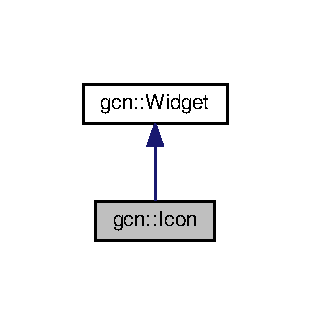
\includegraphics[width=149pt]{classgcn_1_1Icon__inherit__graph}
\end{center}
\end{figure}


Collaboration diagram for gcn\+:\+:Icon\+:\nopagebreak
\begin{figure}[H]
\begin{center}
\leavevmode
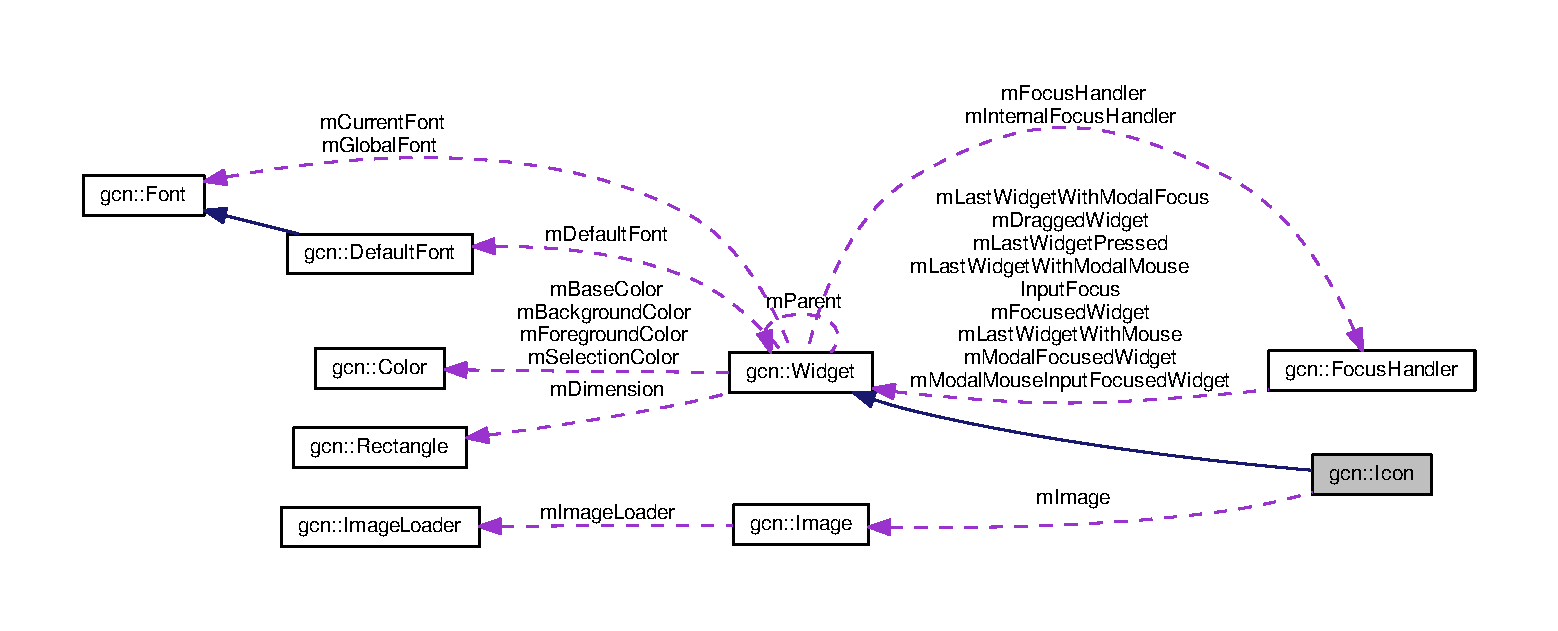
\includegraphics[width=350pt]{classgcn_1_1Icon__coll__graph}
\end{center}
\end{figure}
\subsection*{Public Member Functions}
\begin{DoxyCompactItemize}
\item 
\hyperlink{classgcn_1_1Icon_ade352edc3f6c185035db9c642006fbd3}{Icon} (const std\+::string \&filename)
\item 
\hyperlink{classgcn_1_1Icon_a4dcc025bfd07f33f829f020dcc3298f0}{Icon} (\hyperlink{classgcn_1_1Image}{Image} $\ast$image)
\item 
virtual \hyperlink{classgcn_1_1Icon_a3d626c3c0768ed5d6ba8631aee79ea58}{$\sim$\+Icon} ()
\item 
virtual void \hyperlink{classgcn_1_1Icon_ac490339b9e1824a291a5da93581215d1}{draw} (\hyperlink{classgcn_1_1Graphics}{Graphics} $\ast$graphics)
\item 
virtual void \hyperlink{classgcn_1_1Icon_a1533b6c01b209ff077b9fc37af364db7}{draw\+Border} (\hyperlink{classgcn_1_1Graphics}{Graphics} $\ast$graphics)
\end{DoxyCompactItemize}
\subsection*{Protected Attributes}
\begin{DoxyCompactItemize}
\item 
\hyperlink{classgcn_1_1Image}{Image} $\ast$ \hyperlink{classgcn_1_1Icon_afeed96d96fc1f8cbe51fff7a1933dcc7}{m\+Image}
\item 
bool \hyperlink{classgcn_1_1Icon_add136055bf50bf4cf6da058903d89239}{m\+Internal\+Image}
\end{DoxyCompactItemize}
\subsection*{Additional Inherited Members}


\subsection{Detailed Description}
Implements an icon capable of displaying an image. 

\subsection{Constructor \& Destructor Documentation}
\index{gcn\+::\+Icon@{gcn\+::\+Icon}!Icon@{Icon}}
\index{Icon@{Icon}!gcn\+::\+Icon@{gcn\+::\+Icon}}
\subsubsection[{\texorpdfstring{Icon(const std\+::string \&filename)}{Icon(const std::string &filename)}}]{\setlength{\rightskip}{0pt plus 5cm}gcn\+::\+Icon\+::\+Icon (
\begin{DoxyParamCaption}
\item[{const std\+::string \&}]{filename}
\end{DoxyParamCaption}
)}\hypertarget{classgcn_1_1Icon_ade352edc3f6c185035db9c642006fbd3}{}\label{classgcn_1_1Icon_ade352edc3f6c185035db9c642006fbd3}
Constructor.


\begin{DoxyParams}{Parameters}
{\em filename} & The filename of the image to display. \\
\hline
\end{DoxyParams}
\index{gcn\+::\+Icon@{gcn\+::\+Icon}!Icon@{Icon}}
\index{Icon@{Icon}!gcn\+::\+Icon@{gcn\+::\+Icon}}
\subsubsection[{\texorpdfstring{Icon(\+Image $\ast$image)}{Icon(Image *image)}}]{\setlength{\rightskip}{0pt plus 5cm}gcn\+::\+Icon\+::\+Icon (
\begin{DoxyParamCaption}
\item[{{\bf Image} $\ast$}]{image}
\end{DoxyParamCaption}
)}\hypertarget{classgcn_1_1Icon_a4dcc025bfd07f33f829f020dcc3298f0}{}\label{classgcn_1_1Icon_a4dcc025bfd07f33f829f020dcc3298f0}
Constructor.


\begin{DoxyParams}{Parameters}
{\em image} & The image to display. \\
\hline
\end{DoxyParams}
\index{gcn\+::\+Icon@{gcn\+::\+Icon}!````~Icon@{$\sim$\+Icon}}
\index{````~Icon@{$\sim$\+Icon}!gcn\+::\+Icon@{gcn\+::\+Icon}}
\subsubsection[{\texorpdfstring{$\sim$\+Icon()}{~Icon()}}]{\setlength{\rightskip}{0pt plus 5cm}gcn\+::\+Icon\+::$\sim$\+Icon (
\begin{DoxyParamCaption}
{}
\end{DoxyParamCaption}
)\hspace{0.3cm}{\ttfamily [virtual]}}\hypertarget{classgcn_1_1Icon_a3d626c3c0768ed5d6ba8631aee79ea58}{}\label{classgcn_1_1Icon_a3d626c3c0768ed5d6ba8631aee79ea58}
Descructor. 

\subsection{Member Function Documentation}
\index{gcn\+::\+Icon@{gcn\+::\+Icon}!draw@{draw}}
\index{draw@{draw}!gcn\+::\+Icon@{gcn\+::\+Icon}}
\subsubsection[{\texorpdfstring{draw(\+Graphics $\ast$graphics)}{draw(Graphics *graphics)}}]{\setlength{\rightskip}{0pt plus 5cm}void gcn\+::\+Icon\+::draw (
\begin{DoxyParamCaption}
\item[{{\bf Graphics} $\ast$}]{graphics}
\end{DoxyParamCaption}
)\hspace{0.3cm}{\ttfamily [virtual]}}\hypertarget{classgcn_1_1Icon_ac490339b9e1824a291a5da93581215d1}{}\label{classgcn_1_1Icon_ac490339b9e1824a291a5da93581215d1}
Draws the widget. It is called by the parent widget when it is time for the widget to draw itself. The graphics object is set up so that all drawing is relative to the widget, i.\+e coordinate (0,0) is the top-\/left corner of the widget. It is not possible to draw outside of a widgets dimension.


\begin{DoxyParams}{Parameters}
{\em graphics} & a \hyperlink{classgcn_1_1Graphics}{Graphics} object to draw with. \\
\hline
\end{DoxyParams}


Implements \hyperlink{classgcn_1_1Widget_acc595221d6a2d1afe1043c16dc37d212}{gcn\+::\+Widget}.

\index{gcn\+::\+Icon@{gcn\+::\+Icon}!draw\+Border@{draw\+Border}}
\index{draw\+Border@{draw\+Border}!gcn\+::\+Icon@{gcn\+::\+Icon}}
\subsubsection[{\texorpdfstring{draw\+Border(\+Graphics $\ast$graphics)}{drawBorder(Graphics *graphics)}}]{\setlength{\rightskip}{0pt plus 5cm}void gcn\+::\+Icon\+::draw\+Border (
\begin{DoxyParamCaption}
\item[{{\bf Graphics} $\ast$}]{graphics}
\end{DoxyParamCaption}
)\hspace{0.3cm}{\ttfamily [virtual]}}\hypertarget{classgcn_1_1Icon_a1533b6c01b209ff077b9fc37af364db7}{}\label{classgcn_1_1Icon_a1533b6c01b209ff077b9fc37af364db7}
Draws the widget border. A border is drawn around a widget. The width and height of the border is therefore the widgets height+2$\ast$bordersize. Think of a painting that has a certain size, the border surrounds the painting.


\begin{DoxyParams}{Parameters}
{\em graphics} & a \hyperlink{classgcn_1_1Graphics}{Graphics} object to draw with. \\
\hline
\end{DoxyParams}


Reimplemented from \hyperlink{classgcn_1_1Widget_a58c3b2f513d8e029e321fd88a974f5c4}{gcn\+::\+Widget}.



\subsection{Member Data Documentation}
\index{gcn\+::\+Icon@{gcn\+::\+Icon}!m\+Image@{m\+Image}}
\index{m\+Image@{m\+Image}!gcn\+::\+Icon@{gcn\+::\+Icon}}
\subsubsection[{\texorpdfstring{m\+Image}{mImage}}]{\setlength{\rightskip}{0pt plus 5cm}{\bf Image}$\ast$ gcn\+::\+Icon\+::m\+Image\hspace{0.3cm}{\ttfamily [protected]}}\hypertarget{classgcn_1_1Icon_afeed96d96fc1f8cbe51fff7a1933dcc7}{}\label{classgcn_1_1Icon_afeed96d96fc1f8cbe51fff7a1933dcc7}
The image to display. \index{gcn\+::\+Icon@{gcn\+::\+Icon}!m\+Internal\+Image@{m\+Internal\+Image}}
\index{m\+Internal\+Image@{m\+Internal\+Image}!gcn\+::\+Icon@{gcn\+::\+Icon}}
\subsubsection[{\texorpdfstring{m\+Internal\+Image}{mInternalImage}}]{\setlength{\rightskip}{0pt plus 5cm}bool gcn\+::\+Icon\+::m\+Internal\+Image\hspace{0.3cm}{\ttfamily [protected]}}\hypertarget{classgcn_1_1Icon_add136055bf50bf4cf6da058903d89239}{}\label{classgcn_1_1Icon_add136055bf50bf4cf6da058903d89239}
True if the image has been loaded internally, false otherwise. An image not loaded internally should not be deleted in the destructor. 

The documentation for this class was generated from the following files\+:\begin{DoxyCompactItemize}
\item 
include/guisan/widgets/icon.\+hpp\item 
src/widgets/icon.\+cpp\end{DoxyCompactItemize}

\hypertarget{classgcn_1_1Image}{}\section{gcn\+:\+:Image Class Reference}
\label{classgcn_1_1Image}\index{gcn\+::\+Image@{gcn\+::\+Image}}


{\ttfamily \#include $<$image.\+hpp$>$}



Inheritance diagram for gcn\+:\+:Image\+:\nopagebreak
\begin{figure}[H]
\begin{center}
\leavevmode
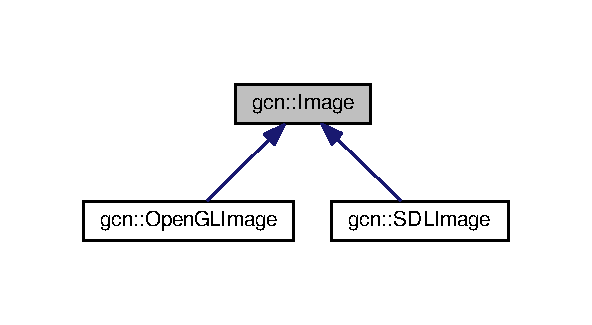
\includegraphics[width=284pt]{classgcn_1_1Image__inherit__graph}
\end{center}
\end{figure}


Collaboration diagram for gcn\+:\+:Image\+:\nopagebreak
\begin{figure}[H]
\begin{center}
\leavevmode
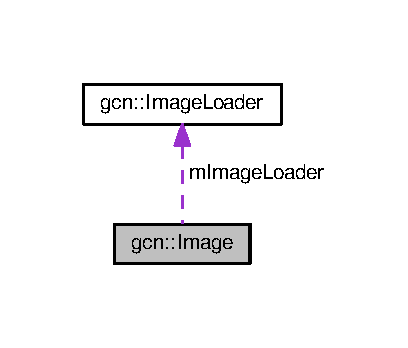
\includegraphics[width=196pt]{classgcn_1_1Image__coll__graph}
\end{center}
\end{figure}
\subsection*{Public Member Functions}
\begin{DoxyCompactItemize}
\item 
\hyperlink{classgcn_1_1Image_a883e7a2a2f9fdf12b671bbbcb31eb75d}{Image} ()
\item 
virtual \hyperlink{classgcn_1_1Image_aea3f86f45826db27d628bffb3c6bd26c}{$\sim$\+Image} ()
\item 
virtual void \hyperlink{classgcn_1_1Image_acfa8910bae0ed3402e9f1f9876e4c4cf}{free} ()=0
\item 
virtual int \hyperlink{classgcn_1_1Image_aa367cc8121c1f01a541e615b0a27497c}{get\+Width} () const =0
\item 
virtual int \hyperlink{classgcn_1_1Image_a09df6a36dc5a76a75a0dd5720f40ee0d}{get\+Height} () const =0
\item 
virtual \hyperlink{classgcn_1_1Color}{Color} \hyperlink{classgcn_1_1Image_a38e79120cc9f81bb36727e2859e04a09}{get\+Pixel} (int x, int y)=0
\item 
virtual void \hyperlink{classgcn_1_1Image_a4a023341cacd32ca4448ceec4b79be4a}{put\+Pixel} (int x, int y, const \hyperlink{classgcn_1_1Color}{Color} \&color)=0
\item 
virtual void \hyperlink{classgcn_1_1Image_a3e59862b9a8fdb2bd3cffd9ba39969af}{convert\+To\+Display\+Format} ()=0
\end{DoxyCompactItemize}
\subsection*{Static Public Member Functions}
\begin{DoxyCompactItemize}
\item 
static \hyperlink{classgcn_1_1Image}{Image} $\ast$ \hyperlink{classgcn_1_1Image_ad48bad2ddf8375c222e3731776baa786}{load} (const std\+::string \&filename, bool \hyperlink{classgcn_1_1Image_a3e59862b9a8fdb2bd3cffd9ba39969af}{convert\+To\+Display\+Format}=true)
\item 
static \hyperlink{classgcn_1_1ImageLoader}{Image\+Loader} $\ast$ \hyperlink{classgcn_1_1Image_ae7660b0958594f7d2287c887c71d3e2d}{get\+Image\+Loader} ()
\item 
static void \hyperlink{classgcn_1_1Image_aa042ca170fcce7fa019eed5475319d62}{set\+Image\+Loader} (\hyperlink{classgcn_1_1ImageLoader}{Image\+Loader} $\ast$image\+Loader)
\end{DoxyCompactItemize}
\subsection*{Static Protected Attributes}
\begin{DoxyCompactItemize}
\item 
static \hyperlink{classgcn_1_1ImageLoader}{Image\+Loader} $\ast$ {\bfseries m\+Image\+Loader} = N\+U\+LL\hypertarget{classgcn_1_1Image_a0226932e40506e397d416d9c253c018b}{}\label{classgcn_1_1Image_a0226932e40506e397d416d9c253c018b}

\end{DoxyCompactItemize}


\subsection{Detailed Description}
Holds an image. To be able to use this class you must first set an \hyperlink{classgcn_1_1ImageLoader}{Image\+Loader} in \hyperlink{classgcn_1_1Image}{Image} by calling 
\begin{DoxyCode}
\hyperlink{classgcn_1_1Image_aa042ca170fcce7fa019eed5475319d62}{Image::setImageLoader}(myImageLoader) 
\end{DoxyCode}
 The function is static. If this is not done, the constructor taking a filename will throw an exception. The \hyperlink{classgcn_1_1ImageLoader}{Image\+Loader} you use must be compatible with the \hyperlink{classgcn_1_1Graphics}{Graphics} object you use.

E\+X\+A\+M\+P\+LE\+: If you use \hyperlink{classgcn_1_1SDLGraphics}{S\+D\+L\+Graphics} you should use \hyperlink{classgcn_1_1SDLImageLoader}{S\+D\+L\+Image\+Loader}. Otherwise your program will crash in a most bizarre way. 

\subsection{Constructor \& Destructor Documentation}
\index{gcn\+::\+Image@{gcn\+::\+Image}!Image@{Image}}
\index{Image@{Image}!gcn\+::\+Image@{gcn\+::\+Image}}
\subsubsection[{\texorpdfstring{Image()}{Image()}}]{\setlength{\rightskip}{0pt plus 5cm}gcn\+::\+Image\+::\+Image (
\begin{DoxyParamCaption}
{}
\end{DoxyParamCaption}
)}\hypertarget{classgcn_1_1Image_a883e7a2a2f9fdf12b671bbbcb31eb75d}{}\label{classgcn_1_1Image_a883e7a2a2f9fdf12b671bbbcb31eb75d}
Constructor. \index{gcn\+::\+Image@{gcn\+::\+Image}!````~Image@{$\sim$\+Image}}
\index{````~Image@{$\sim$\+Image}!gcn\+::\+Image@{gcn\+::\+Image}}
\subsubsection[{\texorpdfstring{$\sim$\+Image()}{~Image()}}]{\setlength{\rightskip}{0pt plus 5cm}gcn\+::\+Image\+::$\sim$\+Image (
\begin{DoxyParamCaption}
{}
\end{DoxyParamCaption}
)\hspace{0.3cm}{\ttfamily [virtual]}}\hypertarget{classgcn_1_1Image_aea3f86f45826db27d628bffb3c6bd26c}{}\label{classgcn_1_1Image_aea3f86f45826db27d628bffb3c6bd26c}
Destructor. 

\subsection{Member Function Documentation}
\index{gcn\+::\+Image@{gcn\+::\+Image}!convert\+To\+Display\+Format@{convert\+To\+Display\+Format}}
\index{convert\+To\+Display\+Format@{convert\+To\+Display\+Format}!gcn\+::\+Image@{gcn\+::\+Image}}
\subsubsection[{\texorpdfstring{convert\+To\+Display\+Format()=0}{convertToDisplayFormat()=0}}]{\setlength{\rightskip}{0pt plus 5cm}virtual void gcn\+::\+Image\+::convert\+To\+Display\+Format (
\begin{DoxyParamCaption}
{}
\end{DoxyParamCaption}
)\hspace{0.3cm}{\ttfamily [pure virtual]}}\hypertarget{classgcn_1_1Image_a3e59862b9a8fdb2bd3cffd9ba39969af}{}\label{classgcn_1_1Image_a3e59862b9a8fdb2bd3cffd9ba39969af}
Converts the image, if possible, to display format.

I\+M\+P\+O\+R\+T\+A\+NT\+: Only guaranteed to work before the image has been converted to display format. 

Implemented in \hyperlink{classgcn_1_1OpenGLImage_a1f1f25745fb9a89a06db56b3e6b2748e}{gcn\+::\+Open\+G\+L\+Image}, and \hyperlink{classgcn_1_1SDLImage_ad9b2c696a7c58af497c3830ad9d76861}{gcn\+::\+S\+D\+L\+Image}.

\index{gcn\+::\+Image@{gcn\+::\+Image}!free@{free}}
\index{free@{free}!gcn\+::\+Image@{gcn\+::\+Image}}
\subsubsection[{\texorpdfstring{free()=0}{free()=0}}]{\setlength{\rightskip}{0pt plus 5cm}virtual void gcn\+::\+Image\+::free (
\begin{DoxyParamCaption}
{}
\end{DoxyParamCaption}
)\hspace{0.3cm}{\ttfamily [pure virtual]}}\hypertarget{classgcn_1_1Image_acfa8910bae0ed3402e9f1f9876e4c4cf}{}\label{classgcn_1_1Image_acfa8910bae0ed3402e9f1f9876e4c4cf}
Frees an image. 

Implemented in \hyperlink{classgcn_1_1OpenGLImage_a5ca72fa90e8f913bbfa37dd067e2c56a}{gcn\+::\+Open\+G\+L\+Image}, and \hyperlink{classgcn_1_1SDLImage_a3bc4ad47bfe36987a48226a676f9f576}{gcn\+::\+S\+D\+L\+Image}.

\index{gcn\+::\+Image@{gcn\+::\+Image}!get\+Height@{get\+Height}}
\index{get\+Height@{get\+Height}!gcn\+::\+Image@{gcn\+::\+Image}}
\subsubsection[{\texorpdfstring{get\+Height() const =0}{getHeight() const =0}}]{\setlength{\rightskip}{0pt plus 5cm}virtual int gcn\+::\+Image\+::get\+Height (
\begin{DoxyParamCaption}
{}
\end{DoxyParamCaption}
) const\hspace{0.3cm}{\ttfamily [pure virtual]}}\hypertarget{classgcn_1_1Image_a09df6a36dc5a76a75a0dd5720f40ee0d}{}\label{classgcn_1_1Image_a09df6a36dc5a76a75a0dd5720f40ee0d}
Gets the height of the \hyperlink{classgcn_1_1Image}{Image}.

\begin{DoxyReturn}{Returns}
the image height 
\end{DoxyReturn}


Implemented in \hyperlink{classgcn_1_1OpenGLImage_a88ecce91748e69434abf055404f5b306}{gcn\+::\+Open\+G\+L\+Image}, and \hyperlink{classgcn_1_1SDLImage_a92002975749328bf9c46c6a647b949d9}{gcn\+::\+S\+D\+L\+Image}.

\index{gcn\+::\+Image@{gcn\+::\+Image}!get\+Image\+Loader@{get\+Image\+Loader}}
\index{get\+Image\+Loader@{get\+Image\+Loader}!gcn\+::\+Image@{gcn\+::\+Image}}
\subsubsection[{\texorpdfstring{get\+Image\+Loader()}{getImageLoader()}}]{\setlength{\rightskip}{0pt plus 5cm}{\bf Image\+Loader} $\ast$ gcn\+::\+Image\+::get\+Image\+Loader (
\begin{DoxyParamCaption}
{}
\end{DoxyParamCaption}
)\hspace{0.3cm}{\ttfamily [static]}}\hypertarget{classgcn_1_1Image_ae7660b0958594f7d2287c887c71d3e2d}{}\label{classgcn_1_1Image_ae7660b0958594f7d2287c887c71d3e2d}
Gets the \hyperlink{classgcn_1_1ImageLoader}{Image\+Loader} used for loading Images.

\begin{DoxyReturn}{Returns}
the \hyperlink{classgcn_1_1ImageLoader}{Image\+Loader} used for loading Images. 
\end{DoxyReturn}
\begin{DoxySeeAlso}{See also}
\hyperlink{classgcn_1_1SDLImageLoader}{S\+D\+L\+Image\+Loader}, Allegro\+Image\+Loader 
\end{DoxySeeAlso}
\index{gcn\+::\+Image@{gcn\+::\+Image}!get\+Pixel@{get\+Pixel}}
\index{get\+Pixel@{get\+Pixel}!gcn\+::\+Image@{gcn\+::\+Image}}
\subsubsection[{\texorpdfstring{get\+Pixel(int x, int y)=0}{getPixel(int x, int y)=0}}]{\setlength{\rightskip}{0pt plus 5cm}virtual {\bf Color} gcn\+::\+Image\+::get\+Pixel (
\begin{DoxyParamCaption}
\item[{int}]{x, }
\item[{int}]{y}
\end{DoxyParamCaption}
)\hspace{0.3cm}{\ttfamily [pure virtual]}}\hypertarget{classgcn_1_1Image_a38e79120cc9f81bb36727e2859e04a09}{}\label{classgcn_1_1Image_a38e79120cc9f81bb36727e2859e04a09}
Gets the color of a pixel at coordinate (x, y) in the image.

I\+M\+P\+O\+R\+T\+A\+NT\+: Only guaranteed to work before the image has been converted to display format.


\begin{DoxyParams}{Parameters}
{\em x} & the x coordinate. \\
\hline
{\em y} & the y coordinate. \\
\hline
\end{DoxyParams}
\begin{DoxyReturn}{Returns}
the color of the pixel. 
\end{DoxyReturn}


Implemented in \hyperlink{classgcn_1_1OpenGLImage_a68af180d0683001cdf1b49fd36d15cfc}{gcn\+::\+Open\+G\+L\+Image}, and \hyperlink{classgcn_1_1SDLImage_af6f2df0d39d68b7c0547943f368f3726}{gcn\+::\+S\+D\+L\+Image}.

\index{gcn\+::\+Image@{gcn\+::\+Image}!get\+Width@{get\+Width}}
\index{get\+Width@{get\+Width}!gcn\+::\+Image@{gcn\+::\+Image}}
\subsubsection[{\texorpdfstring{get\+Width() const =0}{getWidth() const =0}}]{\setlength{\rightskip}{0pt plus 5cm}virtual int gcn\+::\+Image\+::get\+Width (
\begin{DoxyParamCaption}
{}
\end{DoxyParamCaption}
) const\hspace{0.3cm}{\ttfamily [pure virtual]}}\hypertarget{classgcn_1_1Image_aa367cc8121c1f01a541e615b0a27497c}{}\label{classgcn_1_1Image_aa367cc8121c1f01a541e615b0a27497c}
Gets the width of the \hyperlink{classgcn_1_1Image}{Image}.

\begin{DoxyReturn}{Returns}
the image width 
\end{DoxyReturn}


Implemented in \hyperlink{classgcn_1_1OpenGLImage_ad4c50cb4ecbee9dab3e2894dd650a31c}{gcn\+::\+Open\+G\+L\+Image}, and \hyperlink{classgcn_1_1SDLImage_aedda43f210a3e661685636684977eb1e}{gcn\+::\+S\+D\+L\+Image}.

\index{gcn\+::\+Image@{gcn\+::\+Image}!load@{load}}
\index{load@{load}!gcn\+::\+Image@{gcn\+::\+Image}}
\subsubsection[{\texorpdfstring{load(const std\+::string \&filename, bool convert\+To\+Display\+Format=true)}{load(const std::string &filename, bool convertToDisplayFormat=true)}}]{\setlength{\rightskip}{0pt plus 5cm}{\bf Image} $\ast$ gcn\+::\+Image\+::load (
\begin{DoxyParamCaption}
\item[{const std\+::string \&}]{filename, }
\item[{bool}]{convert\+To\+Display\+Format = {\ttfamily true}}
\end{DoxyParamCaption}
)\hspace{0.3cm}{\ttfamily [static]}}\hypertarget{classgcn_1_1Image_ad48bad2ddf8375c222e3731776baa786}{}\label{classgcn_1_1Image_ad48bad2ddf8375c222e3731776baa786}
Loads an image by calling the \hyperlink{classgcn_1_1Image}{Image} class\textquotesingle{} \hyperlink{classgcn_1_1ImageLoader}{Image\+Loader}.

N\+O\+TE\+: The functions get\+Pixel and put\+Pixel are only guaranteed to work before an image has been converted to display format.


\begin{DoxyParams}{Parameters}
{\em filename} & the file to load. \\
\hline
{\em convert\+To\+Display\+Format} & true if the image should be converted to display, false otherwise. \\
\hline
\end{DoxyParams}
\index{gcn\+::\+Image@{gcn\+::\+Image}!put\+Pixel@{put\+Pixel}}
\index{put\+Pixel@{put\+Pixel}!gcn\+::\+Image@{gcn\+::\+Image}}
\subsubsection[{\texorpdfstring{put\+Pixel(int x, int y, const Color \&color)=0}{putPixel(int x, int y, const Color &color)=0}}]{\setlength{\rightskip}{0pt plus 5cm}virtual void gcn\+::\+Image\+::put\+Pixel (
\begin{DoxyParamCaption}
\item[{int}]{x, }
\item[{int}]{y, }
\item[{const {\bf Color} \&}]{color}
\end{DoxyParamCaption}
)\hspace{0.3cm}{\ttfamily [pure virtual]}}\hypertarget{classgcn_1_1Image_a4a023341cacd32ca4448ceec4b79be4a}{}\label{classgcn_1_1Image_a4a023341cacd32ca4448ceec4b79be4a}
Puts a pixel with a certain color at coordinate (x, y).


\begin{DoxyParams}{Parameters}
{\em x} & the x coordinate. \\
\hline
{\em y} & the y coordinate. \\
\hline
{\em color} & the color of the pixel to put. \\
\hline
\end{DoxyParams}


Implemented in \hyperlink{classgcn_1_1OpenGLImage_a8dde453536853dbfc3ea62b21744655b}{gcn\+::\+Open\+G\+L\+Image}, and \hyperlink{classgcn_1_1SDLImage_a707af6ce207dff83174dd91dfd4b4148}{gcn\+::\+S\+D\+L\+Image}.

\index{gcn\+::\+Image@{gcn\+::\+Image}!set\+Image\+Loader@{set\+Image\+Loader}}
\index{set\+Image\+Loader@{set\+Image\+Loader}!gcn\+::\+Image@{gcn\+::\+Image}}
\subsubsection[{\texorpdfstring{set\+Image\+Loader(\+Image\+Loader $\ast$image\+Loader)}{setImageLoader(ImageLoader *imageLoader)}}]{\setlength{\rightskip}{0pt plus 5cm}void gcn\+::\+Image\+::set\+Image\+Loader (
\begin{DoxyParamCaption}
\item[{{\bf Image\+Loader} $\ast$}]{image\+Loader}
\end{DoxyParamCaption}
)\hspace{0.3cm}{\ttfamily [static]}}\hypertarget{classgcn_1_1Image_aa042ca170fcce7fa019eed5475319d62}{}\label{classgcn_1_1Image_aa042ca170fcce7fa019eed5475319d62}
Sets the \hyperlink{classgcn_1_1ImageLoader}{Image\+Loader} to be used for loading images.

I\+M\+P\+O\+R\+T\+A\+NT\+: The \hyperlink{classgcn_1_1ImageLoader}{Image\+Loader} is static and M\+U\+ST be set before loading images!


\begin{DoxyParams}{Parameters}
{\em image\+Loader} & the \hyperlink{classgcn_1_1ImageLoader}{Image\+Loader} to be used for loading images. \\
\hline
\end{DoxyParams}
\begin{DoxySeeAlso}{See also}
\hyperlink{classgcn_1_1SDLImageLoader}{S\+D\+L\+Image\+Loader}, Allegro\+Image\+Loader 
\end{DoxySeeAlso}


The documentation for this class was generated from the following files\+:\begin{DoxyCompactItemize}
\item 
include/guisan/image.\+hpp\item 
src/image.\+cpp\end{DoxyCompactItemize}

\hypertarget{classgcn_1_1ImageButton}{}\section{gcn\+:\+:Image\+Button Class Reference}
\label{classgcn_1_1ImageButton}\index{gcn\+::\+Image\+Button@{gcn\+::\+Image\+Button}}


{\ttfamily \#include $<$imagebutton.\+hpp$>$}



Inheritance diagram for gcn\+:\+:Image\+Button\+:\nopagebreak
\begin{figure}[H]
\begin{center}
\leavevmode
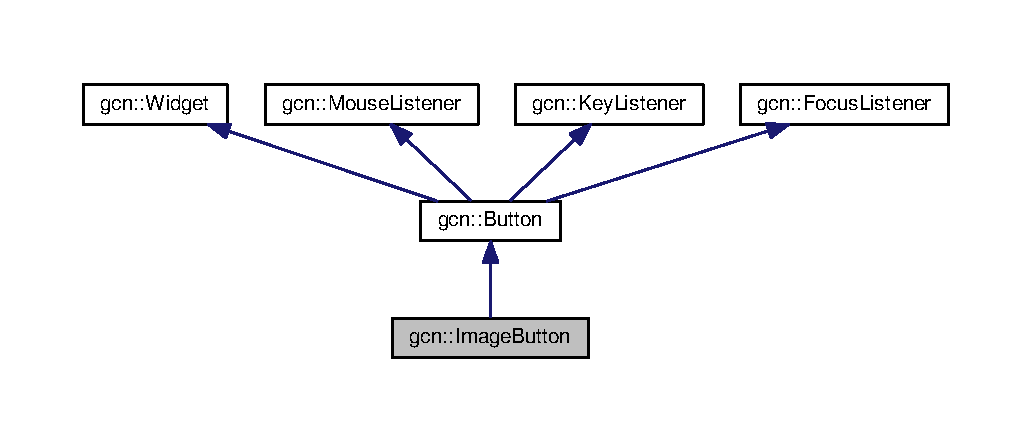
\includegraphics[width=350pt]{classgcn_1_1ImageButton__inherit__graph}
\end{center}
\end{figure}


Collaboration diagram for gcn\+:\+:Image\+Button\+:\nopagebreak
\begin{figure}[H]
\begin{center}
\leavevmode
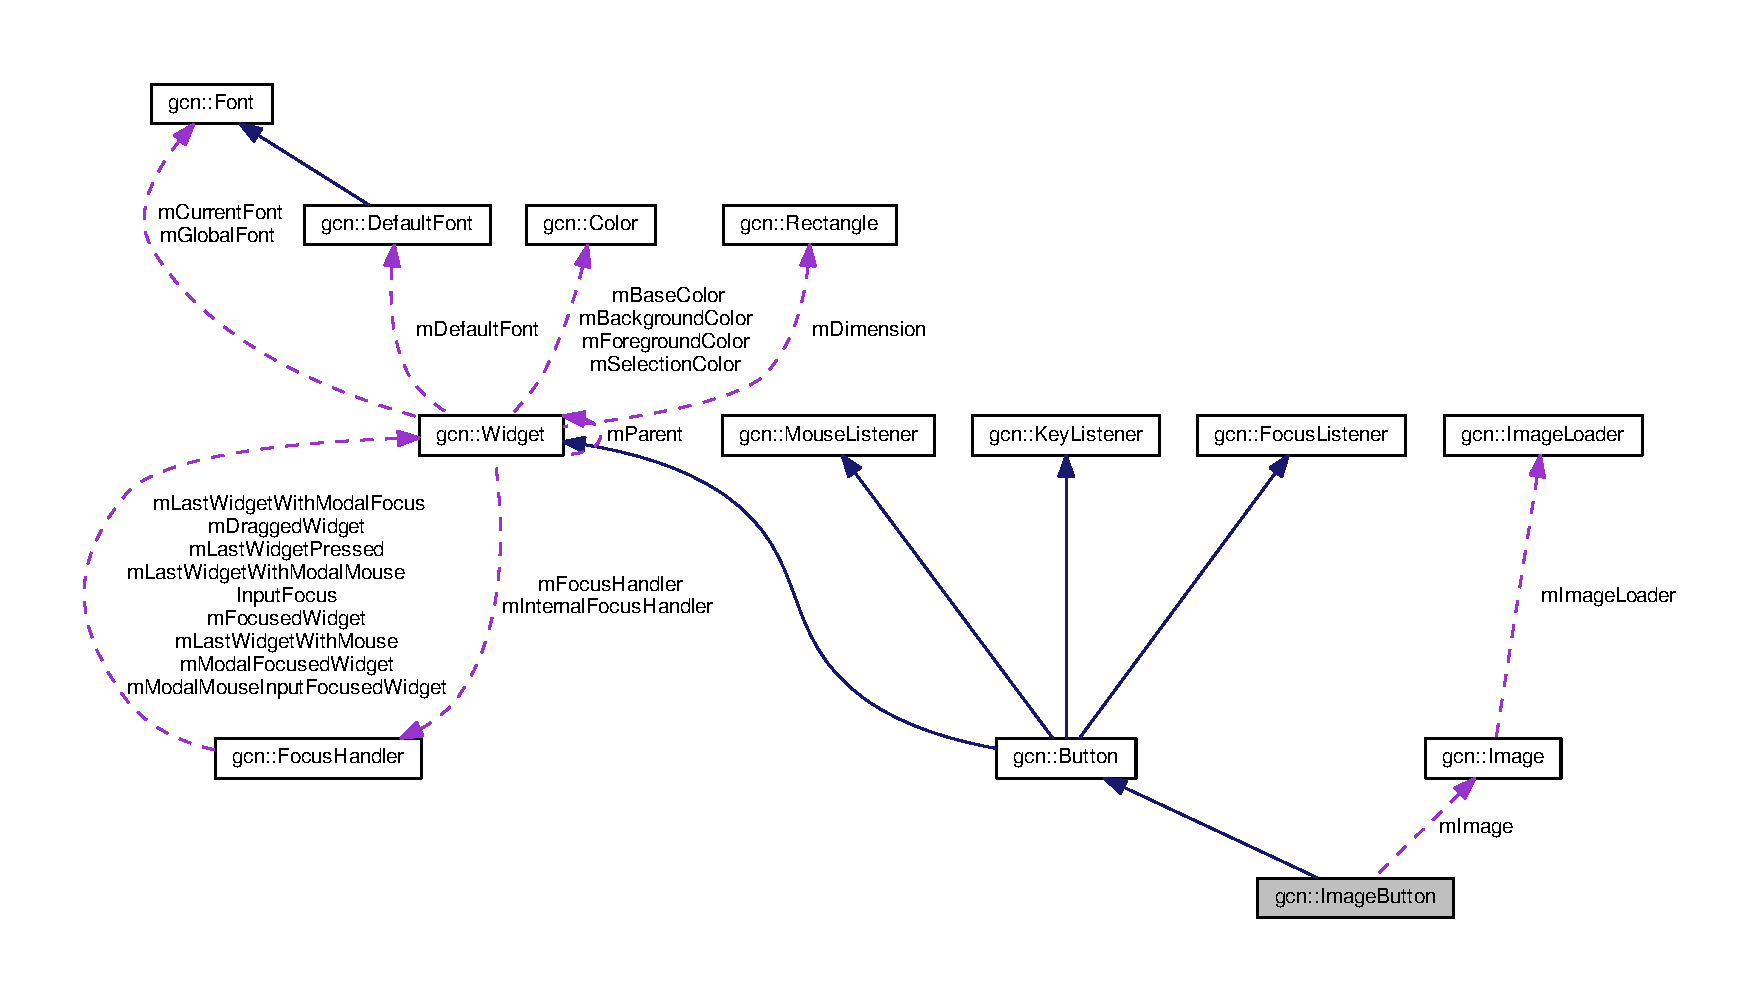
\includegraphics[width=350pt]{classgcn_1_1ImageButton__coll__graph}
\end{center}
\end{figure}
\subsection*{Public Member Functions}
\begin{DoxyCompactItemize}
\item 
\hyperlink{classgcn_1_1ImageButton_a54da62f658134fc699d4ae806f4412e6}{Image\+Button} (const std\+::string \&filename)
\item 
\hyperlink{classgcn_1_1ImageButton_a9186ef6e694608195576ef2bc06e8011}{Image\+Button} (\hyperlink{classgcn_1_1Image}{Image} $\ast$image)
\item 
virtual \hyperlink{classgcn_1_1ImageButton_a0cdce026743d26b826c1be62b69f08cf}{$\sim$\+Image\+Button} ()
\item 
void \hyperlink{classgcn_1_1ImageButton_a5ab1a6bebc05437c4c366989dc2b8f0b}{adjust\+Size} ()
\item 
void \hyperlink{classgcn_1_1ImageButton_ae2c285107583baa3232dee18e3f396a6}{set\+Image} (\hyperlink{classgcn_1_1Image}{Image} $\ast$image)
\item 
\hyperlink{classgcn_1_1Image}{Image} $\ast$ \hyperlink{classgcn_1_1ImageButton_ac1730921714aae0893366137fe775ff0}{get\+Image} ()
\item 
void \hyperlink{classgcn_1_1ImageButton_a067e502ef22fa2f443c575aca9cfe179}{draw} (\hyperlink{classgcn_1_1Graphics}{gcn\+::\+Graphics} $\ast$graphics)
\end{DoxyCompactItemize}
\subsection*{Protected Attributes}
\begin{DoxyCompactItemize}
\item 
\hyperlink{classgcn_1_1Image}{gcn\+::\+Image} $\ast$ {\bfseries m\+Image}\hypertarget{classgcn_1_1ImageButton_afc26c98ffb51c5e5eebc3f101375a6cc}{}\label{classgcn_1_1ImageButton_afc26c98ffb51c5e5eebc3f101375a6cc}

\item 
bool \hyperlink{classgcn_1_1ImageButton_a0e8f9179ab310d84934f1093caa66eb6}{m\+Internal\+Image}
\end{DoxyCompactItemize}
\subsection*{Additional Inherited Members}


\subsection{Detailed Description}
A simple button that displays an image instead of a caption. 

\subsection{Constructor \& Destructor Documentation}
\index{gcn\+::\+Image\+Button@{gcn\+::\+Image\+Button}!Image\+Button@{Image\+Button}}
\index{Image\+Button@{Image\+Button}!gcn\+::\+Image\+Button@{gcn\+::\+Image\+Button}}
\subsubsection[{\texorpdfstring{Image\+Button(const std\+::string \&filename)}{ImageButton(const std::string &filename)}}]{\setlength{\rightskip}{0pt plus 5cm}gcn\+::\+Image\+Button\+::\+Image\+Button (
\begin{DoxyParamCaption}
\item[{const std\+::string \&}]{filename}
\end{DoxyParamCaption}
)}\hypertarget{classgcn_1_1ImageButton_a54da62f658134fc699d4ae806f4412e6}{}\label{classgcn_1_1ImageButton_a54da62f658134fc699d4ae806f4412e6}
Constructor.


\begin{DoxyParams}{Parameters}
{\em filename} & The filename of the image to display. \\
\hline
\end{DoxyParams}
\index{gcn\+::\+Image\+Button@{gcn\+::\+Image\+Button}!Image\+Button@{Image\+Button}}
\index{Image\+Button@{Image\+Button}!gcn\+::\+Image\+Button@{gcn\+::\+Image\+Button}}
\subsubsection[{\texorpdfstring{Image\+Button(\+Image $\ast$image)}{ImageButton(Image *image)}}]{\setlength{\rightskip}{0pt plus 5cm}gcn\+::\+Image\+Button\+::\+Image\+Button (
\begin{DoxyParamCaption}
\item[{{\bf Image} $\ast$}]{image}
\end{DoxyParamCaption}
)}\hypertarget{classgcn_1_1ImageButton_a9186ef6e694608195576ef2bc06e8011}{}\label{classgcn_1_1ImageButton_a9186ef6e694608195576ef2bc06e8011}
Constructor.


\begin{DoxyParams}{Parameters}
{\em image} & The image to display. \\
\hline
\end{DoxyParams}
\index{gcn\+::\+Image\+Button@{gcn\+::\+Image\+Button}!````~Image\+Button@{$\sim$\+Image\+Button}}
\index{````~Image\+Button@{$\sim$\+Image\+Button}!gcn\+::\+Image\+Button@{gcn\+::\+Image\+Button}}
\subsubsection[{\texorpdfstring{$\sim$\+Image\+Button()}{~ImageButton()}}]{\setlength{\rightskip}{0pt plus 5cm}gcn\+::\+Image\+Button\+::$\sim$\+Image\+Button (
\begin{DoxyParamCaption}
{}
\end{DoxyParamCaption}
)\hspace{0.3cm}{\ttfamily [virtual]}}\hypertarget{classgcn_1_1ImageButton_a0cdce026743d26b826c1be62b69f08cf}{}\label{classgcn_1_1ImageButton_a0cdce026743d26b826c1be62b69f08cf}
Destructor. 

\subsection{Member Function Documentation}
\index{gcn\+::\+Image\+Button@{gcn\+::\+Image\+Button}!adjust\+Size@{adjust\+Size}}
\index{adjust\+Size@{adjust\+Size}!gcn\+::\+Image\+Button@{gcn\+::\+Image\+Button}}
\subsubsection[{\texorpdfstring{adjust\+Size()}{adjustSize()}}]{\setlength{\rightskip}{0pt plus 5cm}void gcn\+::\+Image\+Button\+::adjust\+Size (
\begin{DoxyParamCaption}
{}
\end{DoxyParamCaption}
)}\hypertarget{classgcn_1_1ImageButton_a5ab1a6bebc05437c4c366989dc2b8f0b}{}\label{classgcn_1_1ImageButton_a5ab1a6bebc05437c4c366989dc2b8f0b}
Adjusts the size of the image button to fit the image. \index{gcn\+::\+Image\+Button@{gcn\+::\+Image\+Button}!draw@{draw}}
\index{draw@{draw}!gcn\+::\+Image\+Button@{gcn\+::\+Image\+Button}}
\subsubsection[{\texorpdfstring{draw(gcn\+::\+Graphics $\ast$graphics)}{draw(gcn::Graphics *graphics)}}]{\setlength{\rightskip}{0pt plus 5cm}void gcn\+::\+Image\+Button\+::draw (
\begin{DoxyParamCaption}
\item[{{\bf gcn\+::\+Graphics} $\ast$}]{graphics}
\end{DoxyParamCaption}
)\hspace{0.3cm}{\ttfamily [virtual]}}\hypertarget{classgcn_1_1ImageButton_a067e502ef22fa2f443c575aca9cfe179}{}\label{classgcn_1_1ImageButton_a067e502ef22fa2f443c575aca9cfe179}
Draws the widget. It is called by the parent widget when it is time for the widget to draw itself. The graphics object is set up so that all drawing is relative to the widget, i.\+e coordinate (0,0) is the top-\/left corner of the widget. It is not possible to draw outside of a widgets dimension.


\begin{DoxyParams}{Parameters}
{\em graphics} & a \hyperlink{classgcn_1_1Graphics}{Graphics} object to draw with. \\
\hline
\end{DoxyParams}


Reimplemented from \hyperlink{classgcn_1_1Button_a741dca35284e5155cd99c1e962e3d1e8}{gcn\+::\+Button}.

\index{gcn\+::\+Image\+Button@{gcn\+::\+Image\+Button}!get\+Image@{get\+Image}}
\index{get\+Image@{get\+Image}!gcn\+::\+Image\+Button@{gcn\+::\+Image\+Button}}
\subsubsection[{\texorpdfstring{get\+Image()}{getImage()}}]{\setlength{\rightskip}{0pt plus 5cm}{\bf Image}$\ast$ gcn\+::\+Image\+Button\+::get\+Image (
\begin{DoxyParamCaption}
{}
\end{DoxyParamCaption}
)}\hypertarget{classgcn_1_1ImageButton_ac1730921714aae0893366137fe775ff0}{}\label{classgcn_1_1ImageButton_ac1730921714aae0893366137fe775ff0}
Gets the image of the image button.

\begin{DoxyReturn}{Returns}
The image of the image button. 
\end{DoxyReturn}
\index{gcn\+::\+Image\+Button@{gcn\+::\+Image\+Button}!set\+Image@{set\+Image}}
\index{set\+Image@{set\+Image}!gcn\+::\+Image\+Button@{gcn\+::\+Image\+Button}}
\subsubsection[{\texorpdfstring{set\+Image(\+Image $\ast$image)}{setImage(Image *image)}}]{\setlength{\rightskip}{0pt plus 5cm}void gcn\+::\+Image\+Button\+::set\+Image (
\begin{DoxyParamCaption}
\item[{{\bf Image} $\ast$}]{image}
\end{DoxyParamCaption}
)}\hypertarget{classgcn_1_1ImageButton_ae2c285107583baa3232dee18e3f396a6}{}\label{classgcn_1_1ImageButton_ae2c285107583baa3232dee18e3f396a6}
Sets the image to display.


\begin{DoxyParams}{Parameters}
{\em image} & The image to display. \\
\hline
\end{DoxyParams}


\subsection{Member Data Documentation}
\index{gcn\+::\+Image\+Button@{gcn\+::\+Image\+Button}!m\+Internal\+Image@{m\+Internal\+Image}}
\index{m\+Internal\+Image@{m\+Internal\+Image}!gcn\+::\+Image\+Button@{gcn\+::\+Image\+Button}}
\subsubsection[{\texorpdfstring{m\+Internal\+Image}{mInternalImage}}]{\setlength{\rightskip}{0pt plus 5cm}bool gcn\+::\+Image\+Button\+::m\+Internal\+Image\hspace{0.3cm}{\ttfamily [protected]}}\hypertarget{classgcn_1_1ImageButton_a0e8f9179ab310d84934f1093caa66eb6}{}\label{classgcn_1_1ImageButton_a0e8f9179ab310d84934f1093caa66eb6}
True if the image has been loaded internally, false otherwise. An image not loaded internally should not be deleted in the destructor. 

The documentation for this class was generated from the following files\+:\begin{DoxyCompactItemize}
\item 
include/guisan/widgets/imagebutton.\+hpp\item 
src/widgets/imagebutton.\+cpp\end{DoxyCompactItemize}

\hypertarget{classgcn_1_1ImageFont}{}\section{gcn\+:\+:Image\+Font Class Reference}
\label{classgcn_1_1ImageFont}\index{gcn\+::\+Image\+Font@{gcn\+::\+Image\+Font}}


{\ttfamily \#include $<$imagefont.\+hpp$>$}



Inheritance diagram for gcn\+:\+:Image\+Font\+:\nopagebreak
\begin{figure}[H]
\begin{center}
\leavevmode
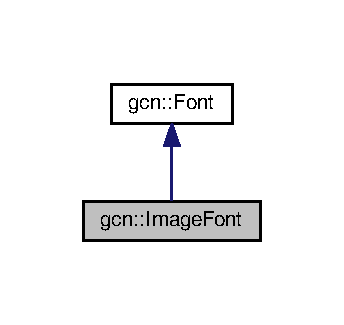
\includegraphics[width=165pt]{classgcn_1_1ImageFont__inherit__graph}
\end{center}
\end{figure}


Collaboration diagram for gcn\+:\+:Image\+Font\+:\nopagebreak
\begin{figure}[H]
\begin{center}
\leavevmode
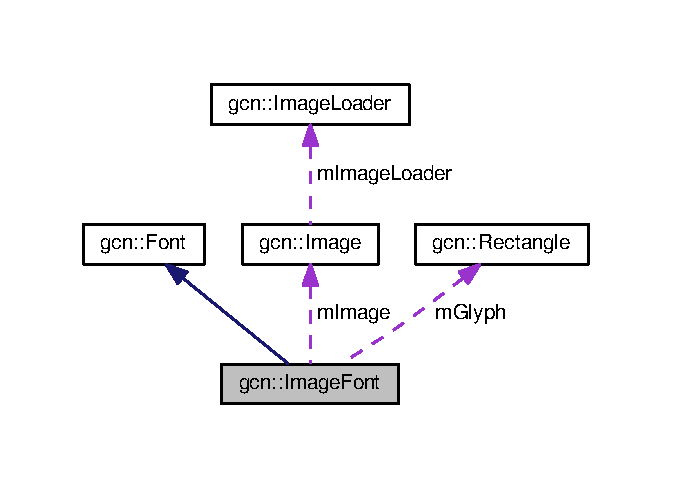
\includegraphics[width=323pt]{classgcn_1_1ImageFont__coll__graph}
\end{center}
\end{figure}
\subsection*{Public Member Functions}
\begin{DoxyCompactItemize}
\item 
\hyperlink{classgcn_1_1ImageFont_a43a623be5f18290c0ba8d6ce886d74b0}{Image\+Font} (const std\+::string \&filename, const std\+::string \&glyphs)
\item 
\hyperlink{classgcn_1_1ImageFont_a663a7535d33714c4dac20518e41a3653}{Image\+Font} (const std\+::string \&filename, unsigned char glyphs\+From=32, unsigned char glyphs\+To=126)
\item 
virtual \hyperlink{classgcn_1_1ImageFont_aa65f1677811e42ecdc747a4196806ea7}{$\sim$\+Image\+Font} ()
\item 
virtual int \hyperlink{classgcn_1_1ImageFont_ab7c08a441ed8046320c600d7eee77bde}{draw\+Glyph} (\hyperlink{classgcn_1_1Graphics}{Graphics} $\ast$graphics, unsigned char glyph, int x, int y)
\item 
virtual void \hyperlink{classgcn_1_1ImageFont_a6fce0fdaa92f10d9e198311e18e1cea3}{set\+Row\+Spacing} (int spacing)
\item 
virtual int \hyperlink{classgcn_1_1ImageFont_abd478dc1dc02a683775a465f21a56cfc}{get\+Row\+Spacing} ()
\item 
virtual void \hyperlink{classgcn_1_1ImageFont_aca8cc062c7b9d232dec6d994a726958e}{set\+Glyph\+Spacing} (int spacing)
\item 
virtual int \hyperlink{classgcn_1_1ImageFont_a3e8595cfdf106632bbc3b55b026d47a5}{get\+Glyph\+Spacing} ()
\item 
virtual int \hyperlink{classgcn_1_1ImageFont_a7f668b99441084f4199982e7d570781d}{get\+Width} (unsigned char glyph) const 
\item 
virtual int \hyperlink{classgcn_1_1ImageFont_a6432c448c9df16a3ca057b2bd9822663}{get\+Width} (const std\+::string \&text) const 
\item 
virtual void \hyperlink{classgcn_1_1ImageFont_a8717f4ef08e2ba1a1379a4b8fe4b5002}{draw\+String} (\hyperlink{classgcn_1_1Graphics}{Graphics} $\ast$graphics, const std\+::string \&text, int x, int y)
\item 
virtual int \hyperlink{classgcn_1_1ImageFont_ae18f2d854e42ce5aafd44e8b8c6ff048}{get\+Height} () const 
\item 
virtual int \hyperlink{classgcn_1_1ImageFont_a5b0e7a7a7acdcb9fadb232f63608b354}{get\+String\+Index\+At} (const std\+::string \&text, int x)
\end{DoxyCompactItemize}
\subsection*{Protected Member Functions}
\begin{DoxyCompactItemize}
\item 
void {\bfseries add\+Glyph} (unsigned char c, int \&x, int \&y, const \hyperlink{classgcn_1_1Color}{Color} \&separator)\hypertarget{classgcn_1_1ImageFont_a05f3206435b4b746206ba5f8dc6748ca}{}\label{classgcn_1_1ImageFont_a05f3206435b4b746206ba5f8dc6748ca}

\end{DoxyCompactItemize}
\subsection*{Protected Attributes}
\begin{DoxyCompactItemize}
\item 
\hyperlink{classgcn_1_1Rectangle}{Rectangle} {\bfseries m\+Glyph} \mbox{[}256\mbox{]}\hypertarget{classgcn_1_1ImageFont_abba14f56fa98e464b7a839e432d3c02b}{}\label{classgcn_1_1ImageFont_abba14f56fa98e464b7a839e432d3c02b}

\item 
int {\bfseries m\+Height}\hypertarget{classgcn_1_1ImageFont_ad3d7d7cf93af238d8937b23034061e61}{}\label{classgcn_1_1ImageFont_ad3d7d7cf93af238d8937b23034061e61}

\item 
int {\bfseries m\+Glyph\+Spacing}\hypertarget{classgcn_1_1ImageFont_afb4b350fd417e7dba6ce8f8c14a3b105}{}\label{classgcn_1_1ImageFont_afb4b350fd417e7dba6ce8f8c14a3b105}

\item 
int {\bfseries m\+Row\+Spacing}\hypertarget{classgcn_1_1ImageFont_ab0a6729c8ff035e2755a3215cadfec74}{}\label{classgcn_1_1ImageFont_ab0a6729c8ff035e2755a3215cadfec74}

\item 
\hyperlink{classgcn_1_1Image}{Image} $\ast$ {\bfseries m\+Image}\hypertarget{classgcn_1_1ImageFont_a13409336f029a03e4a5ffe7634854ce3}{}\label{classgcn_1_1ImageFont_a13409336f029a03e4a5ffe7634854ce3}

\item 
std\+::string {\bfseries m\+Filename}\hypertarget{classgcn_1_1ImageFont_ac5ed59920e10fe0d137e365baaf7c568}{}\label{classgcn_1_1ImageFont_ac5ed59920e10fe0d137e365baaf7c568}

\end{DoxyCompactItemize}


\subsection{Detailed Description}
A font using an image containing the font data. It implements the font class. You can use any filetype for the font data as long as it can be loaded with your \hyperlink{classgcn_1_1ImageLoader}{Image\+Loader}.

This are two examples of an image containing a font.  

The \hyperlink{classgcn_1_1Image}{Image} font format works like this\+: The first pixel, the pixal at coordinate (0,0), tells which color to look for when seperating glyphs. You create an image with your glyphs and simple separates them with the seperation color. When you create your \hyperlink{classgcn_1_1ImageFont}{Image\+Font} you supply the constructor with the glyphs present in your image. When creating an \hyperlink{classgcn_1_1ImageFont}{Image\+Font} for the image data in the first example above, the following constructor call would be used. 
\begin{DoxyCode}
 \hyperlink{classgcn_1_1ImageFont}{gcn::ImageFont} imageFont(\textcolor{stringliteral}{"fixedfont\_big.bmp"},\textcolor{stringliteral}{" abcdefghijklmno\(\backslash\)}
\textcolor{stringliteral}{pqrstuvwxyzABCDEFGHIJKLMNOPQRSTUVWXYZ0123456789"}); 
\end{DoxyCode}
 Noteworthy is that the first glyph actually gives the width of space. Glyphs can, as seen in the second example above, be seperated with horizontal lines making it possible to draw glyphs on more then one line in the image. However, these vertical lines must be of one pixel size! 

\subsection{Constructor \& Destructor Documentation}
\index{gcn\+::\+Image\+Font@{gcn\+::\+Image\+Font}!Image\+Font@{Image\+Font}}
\index{Image\+Font@{Image\+Font}!gcn\+::\+Image\+Font@{gcn\+::\+Image\+Font}}
\subsubsection[{\texorpdfstring{Image\+Font(const std\+::string \&filename, const std\+::string \&glyphs)}{ImageFont(const std::string &filename, const std::string &glyphs)}}]{\setlength{\rightskip}{0pt plus 5cm}gcn\+::\+Image\+Font\+::\+Image\+Font (
\begin{DoxyParamCaption}
\item[{const std\+::string \&}]{filename, }
\item[{const std\+::string \&}]{glyphs}
\end{DoxyParamCaption}
)}\hypertarget{classgcn_1_1ImageFont_a43a623be5f18290c0ba8d6ce886d74b0}{}\label{classgcn_1_1ImageFont_a43a623be5f18290c0ba8d6ce886d74b0}
Constructor which takes an image file containing the font and a string containing the glyphs. The glyphs in the string should be in the same order as they appear in the font image.


\begin{DoxyParams}{Parameters}
{\em filename} & the filename of the image. \\
\hline
{\em glyphs} & the glyphs found in the image. \\
\hline
\end{DoxyParams}

\begin{DoxyExceptions}{Exceptions}
{\em \hyperlink{classgcn_1_1Exception}{Exception}} & when glyph list is incorrect or the font file is corrupt or if no \hyperlink{classgcn_1_1ImageLoader}{Image\+Loader} exists. \\
\hline
\end{DoxyExceptions}
\index{gcn\+::\+Image\+Font@{gcn\+::\+Image\+Font}!Image\+Font@{Image\+Font}}
\index{Image\+Font@{Image\+Font}!gcn\+::\+Image\+Font@{gcn\+::\+Image\+Font}}
\subsubsection[{\texorpdfstring{Image\+Font(const std\+::string \&filename, unsigned char glyphs\+From=32, unsigned char glyphs\+To=126)}{ImageFont(const std::string &filename, unsigned char glyphsFrom=32, unsigned char glyphsTo=126)}}]{\setlength{\rightskip}{0pt plus 5cm}gcn\+::\+Image\+Font\+::\+Image\+Font (
\begin{DoxyParamCaption}
\item[{const std\+::string \&}]{filename, }
\item[{unsigned char}]{glyphs\+From = {\ttfamily 32}, }
\item[{unsigned char}]{glyphs\+To = {\ttfamily 126}}
\end{DoxyParamCaption}
)}\hypertarget{classgcn_1_1ImageFont_a663a7535d33714c4dac20518e41a3653}{}\label{classgcn_1_1ImageFont_a663a7535d33714c4dac20518e41a3653}
Constructor which takes an image file containing the font and two boundaries of A\+S\+C\+II values. The font image should include all glyphs specified with the boundaries in increasing A\+S\+C\+II order. The boundaries are inclusive.


\begin{DoxyParams}{Parameters}
{\em filename} & the filename of the image. \\
\hline
{\em glyphs\+From} & the A\+S\+C\+II value of the first glyph found in the image. \\
\hline
{\em glyphs\+To} & the A\+S\+C\+II value of the last glyph found in the image. \\
\hline
\end{DoxyParams}

\begin{DoxyExceptions}{Exceptions}
{\em \hyperlink{classgcn_1_1Exception}{Exception}} & when glyph bondaries are incorrect or the font file is corrupt or if no \hyperlink{classgcn_1_1ImageLoader}{Image\+Loader} exists. \\
\hline
\end{DoxyExceptions}
\index{gcn\+::\+Image\+Font@{gcn\+::\+Image\+Font}!````~Image\+Font@{$\sim$\+Image\+Font}}
\index{````~Image\+Font@{$\sim$\+Image\+Font}!gcn\+::\+Image\+Font@{gcn\+::\+Image\+Font}}
\subsubsection[{\texorpdfstring{$\sim$\+Image\+Font()}{~ImageFont()}}]{\setlength{\rightskip}{0pt plus 5cm}gcn\+::\+Image\+Font\+::$\sim$\+Image\+Font (
\begin{DoxyParamCaption}
{}
\end{DoxyParamCaption}
)\hspace{0.3cm}{\ttfamily [virtual]}}\hypertarget{classgcn_1_1ImageFont_aa65f1677811e42ecdc747a4196806ea7}{}\label{classgcn_1_1ImageFont_aa65f1677811e42ecdc747a4196806ea7}
Destructor. 

\subsection{Member Function Documentation}
\index{gcn\+::\+Image\+Font@{gcn\+::\+Image\+Font}!draw\+Glyph@{draw\+Glyph}}
\index{draw\+Glyph@{draw\+Glyph}!gcn\+::\+Image\+Font@{gcn\+::\+Image\+Font}}
\subsubsection[{\texorpdfstring{draw\+Glyph(\+Graphics $\ast$graphics, unsigned char glyph, int x, int y)}{drawGlyph(Graphics *graphics, unsigned char glyph, int x, int y)}}]{\setlength{\rightskip}{0pt plus 5cm}int gcn\+::\+Image\+Font\+::draw\+Glyph (
\begin{DoxyParamCaption}
\item[{{\bf Graphics} $\ast$}]{graphics, }
\item[{unsigned char}]{glyph, }
\item[{int}]{x, }
\item[{int}]{y}
\end{DoxyParamCaption}
)\hspace{0.3cm}{\ttfamily [virtual]}}\hypertarget{classgcn_1_1ImageFont_ab7c08a441ed8046320c600d7eee77bde}{}\label{classgcn_1_1ImageFont_ab7c08a441ed8046320c600d7eee77bde}
Draws a glyph.

N\+O\+TE\+: You normally won\textquotesingle{}t use this function to draw text since the \hyperlink{classgcn_1_1Graphics}{Graphics} class contains better functions for drawing text.


\begin{DoxyParams}{Parameters}
{\em graphics} & a graphics object to be used for drawing. \\
\hline
{\em glyph} & a glyph to draw. \\
\hline
{\em x} & the x coordinate where to draw the glyph. \\
\hline
{\em y} & the y coordinate where to draw the glyph. \\
\hline
\end{DoxyParams}
\begin{DoxyReturn}{Returns}
the width of the glyph in pixels. 
\end{DoxyReturn}
\begin{DoxySeeAlso}{See also}
\hyperlink{classgcn_1_1Graphics}{Graphics} 
\end{DoxySeeAlso}
\index{gcn\+::\+Image\+Font@{gcn\+::\+Image\+Font}!draw\+String@{draw\+String}}
\index{draw\+String@{draw\+String}!gcn\+::\+Image\+Font@{gcn\+::\+Image\+Font}}
\subsubsection[{\texorpdfstring{draw\+String(\+Graphics $\ast$graphics, const std\+::string \&text, int x, int y)}{drawString(Graphics *graphics, const std::string &text, int x, int y)}}]{\setlength{\rightskip}{0pt plus 5cm}void gcn\+::\+Image\+Font\+::draw\+String (
\begin{DoxyParamCaption}
\item[{{\bf Graphics} $\ast$}]{graphics, }
\item[{const std\+::string \&}]{text, }
\item[{int}]{x, }
\item[{int}]{y}
\end{DoxyParamCaption}
)\hspace{0.3cm}{\ttfamily [virtual]}}\hypertarget{classgcn_1_1ImageFont_a8717f4ef08e2ba1a1379a4b8fe4b5002}{}\label{classgcn_1_1ImageFont_a8717f4ef08e2ba1a1379a4b8fe4b5002}
Draws a string.

N\+O\+TE\+: You normally won\textquotesingle{}t use this function to draw text since \hyperlink{classgcn_1_1Graphics}{Graphics} contains better functions for drawing text.


\begin{DoxyParams}{Parameters}
{\em graphics} & a \hyperlink{classgcn_1_1Graphics}{Graphics} object to use for drawing. \\
\hline
{\em text} & the string to draw. \\
\hline
{\em x} & the x coordinate where to draw the string. \\
\hline
{\em y} & the y coordinate where to draw the string. \\
\hline
\end{DoxyParams}


Implements \hyperlink{classgcn_1_1Font_a055c403050f483cc2c67477443d98eee}{gcn\+::\+Font}.

\index{gcn\+::\+Image\+Font@{gcn\+::\+Image\+Font}!get\+Glyph\+Spacing@{get\+Glyph\+Spacing}}
\index{get\+Glyph\+Spacing@{get\+Glyph\+Spacing}!gcn\+::\+Image\+Font@{gcn\+::\+Image\+Font}}
\subsubsection[{\texorpdfstring{get\+Glyph\+Spacing()}{getGlyphSpacing()}}]{\setlength{\rightskip}{0pt plus 5cm}int gcn\+::\+Image\+Font\+::get\+Glyph\+Spacing (
\begin{DoxyParamCaption}
{}
\end{DoxyParamCaption}
)\hspace{0.3cm}{\ttfamily [virtual]}}\hypertarget{classgcn_1_1ImageFont_a3e8595cfdf106632bbc3b55b026d47a5}{}\label{classgcn_1_1ImageFont_a3e8595cfdf106632bbc3b55b026d47a5}
Gets the spacing between letters in pixels.

\begin{DoxyReturn}{Returns}
the spacing. 
\end{DoxyReturn}
\index{gcn\+::\+Image\+Font@{gcn\+::\+Image\+Font}!get\+Height@{get\+Height}}
\index{get\+Height@{get\+Height}!gcn\+::\+Image\+Font@{gcn\+::\+Image\+Font}}
\subsubsection[{\texorpdfstring{get\+Height() const }{getHeight() const }}]{\setlength{\rightskip}{0pt plus 5cm}int gcn\+::\+Image\+Font\+::get\+Height (
\begin{DoxyParamCaption}
{}
\end{DoxyParamCaption}
) const\hspace{0.3cm}{\ttfamily [virtual]}}\hypertarget{classgcn_1_1ImageFont_ae18f2d854e42ce5aafd44e8b8c6ff048}{}\label{classgcn_1_1ImageFont_ae18f2d854e42ce5aafd44e8b8c6ff048}
Gets the height of the glyphs in the font.

\begin{DoxyReturn}{Returns}
the height of the glyphs int the font. 
\end{DoxyReturn}


Implements \hyperlink{classgcn_1_1Font_aa270d8934a16d4065143e3617b1fa926}{gcn\+::\+Font}.

\index{gcn\+::\+Image\+Font@{gcn\+::\+Image\+Font}!get\+Row\+Spacing@{get\+Row\+Spacing}}
\index{get\+Row\+Spacing@{get\+Row\+Spacing}!gcn\+::\+Image\+Font@{gcn\+::\+Image\+Font}}
\subsubsection[{\texorpdfstring{get\+Row\+Spacing()}{getRowSpacing()}}]{\setlength{\rightskip}{0pt plus 5cm}int gcn\+::\+Image\+Font\+::get\+Row\+Spacing (
\begin{DoxyParamCaption}
{}
\end{DoxyParamCaption}
)\hspace{0.3cm}{\ttfamily [virtual]}}\hypertarget{classgcn_1_1ImageFont_abd478dc1dc02a683775a465f21a56cfc}{}\label{classgcn_1_1ImageFont_abd478dc1dc02a683775a465f21a56cfc}
Gets the spacing between rows in pixels.

\begin{DoxyReturn}{Returns}
the spacing. 
\end{DoxyReturn}
\index{gcn\+::\+Image\+Font@{gcn\+::\+Image\+Font}!get\+String\+Index\+At@{get\+String\+Index\+At}}
\index{get\+String\+Index\+At@{get\+String\+Index\+At}!gcn\+::\+Image\+Font@{gcn\+::\+Image\+Font}}
\subsubsection[{\texorpdfstring{get\+String\+Index\+At(const std\+::string \&text, int x)}{getStringIndexAt(const std::string &text, int x)}}]{\setlength{\rightskip}{0pt plus 5cm}int gcn\+::\+Image\+Font\+::get\+String\+Index\+At (
\begin{DoxyParamCaption}
\item[{const std\+::string \&}]{text, }
\item[{int}]{x}
\end{DoxyParamCaption}
)\hspace{0.3cm}{\ttfamily [virtual]}}\hypertarget{classgcn_1_1ImageFont_a5b0e7a7a7acdcb9fadb232f63608b354}{}\label{classgcn_1_1ImageFont_a5b0e7a7a7acdcb9fadb232f63608b354}
Gets a string index in a string providing an x coordinate. Used to retrive a string index (for a character in a string) at a certain x position. It is especially useful when a mouse clicks in a \hyperlink{classgcn_1_1TextField}{Text\+Field} and you want to know which character was clicked.

\begin{DoxyReturn}{Returns}
a string index in a string providing an x coordinate. 
\end{DoxyReturn}


Reimplemented from \hyperlink{classgcn_1_1Font_a3210f4c53424ade4b188b8dfb1f686a4}{gcn\+::\+Font}.

\index{gcn\+::\+Image\+Font@{gcn\+::\+Image\+Font}!get\+Width@{get\+Width}}
\index{get\+Width@{get\+Width}!gcn\+::\+Image\+Font@{gcn\+::\+Image\+Font}}
\subsubsection[{\texorpdfstring{get\+Width(unsigned char glyph) const }{getWidth(unsigned char glyph) const }}]{\setlength{\rightskip}{0pt plus 5cm}int gcn\+::\+Image\+Font\+::get\+Width (
\begin{DoxyParamCaption}
\item[{unsigned char}]{glyph}
\end{DoxyParamCaption}
) const\hspace{0.3cm}{\ttfamily [virtual]}}\hypertarget{classgcn_1_1ImageFont_a7f668b99441084f4199982e7d570781d}{}\label{classgcn_1_1ImageFont_a7f668b99441084f4199982e7d570781d}
Gets a width of a glyph.


\begin{DoxyParams}{Parameters}
{\em glyph} & the glyph which width will be returned \\
\hline
\end{DoxyParams}
\begin{DoxyReturn}{Returns}
the width of a glyph 
\end{DoxyReturn}
\index{gcn\+::\+Image\+Font@{gcn\+::\+Image\+Font}!get\+Width@{get\+Width}}
\index{get\+Width@{get\+Width}!gcn\+::\+Image\+Font@{gcn\+::\+Image\+Font}}
\subsubsection[{\texorpdfstring{get\+Width(const std\+::string \&text) const }{getWidth(const std::string &text) const }}]{\setlength{\rightskip}{0pt plus 5cm}int gcn\+::\+Image\+Font\+::get\+Width (
\begin{DoxyParamCaption}
\item[{const std\+::string \&}]{text}
\end{DoxyParamCaption}
) const\hspace{0.3cm}{\ttfamily [virtual]}}\hypertarget{classgcn_1_1ImageFont_a6432c448c9df16a3ca057b2bd9822663}{}\label{classgcn_1_1ImageFont_a6432c448c9df16a3ca057b2bd9822663}
Gets the width of a string. The width of a string is not necesserily the sum of all the widths of it\textquotesingle{}s glyphs.


\begin{DoxyParams}{Parameters}
{\em text} & the string to return the width of. \\
\hline
\end{DoxyParams}
\begin{DoxyReturn}{Returns}
the width of a string. 
\end{DoxyReturn}


Implements \hyperlink{classgcn_1_1Font_abb88894b1ebeda28edcac75c537f8e0f}{gcn\+::\+Font}.

\index{gcn\+::\+Image\+Font@{gcn\+::\+Image\+Font}!set\+Glyph\+Spacing@{set\+Glyph\+Spacing}}
\index{set\+Glyph\+Spacing@{set\+Glyph\+Spacing}!gcn\+::\+Image\+Font@{gcn\+::\+Image\+Font}}
\subsubsection[{\texorpdfstring{set\+Glyph\+Spacing(int spacing)}{setGlyphSpacing(int spacing)}}]{\setlength{\rightskip}{0pt plus 5cm}void gcn\+::\+Image\+Font\+::set\+Glyph\+Spacing (
\begin{DoxyParamCaption}
\item[{int}]{spacing}
\end{DoxyParamCaption}
)\hspace{0.3cm}{\ttfamily [virtual]}}\hypertarget{classgcn_1_1ImageFont_aca8cc062c7b9d232dec6d994a726958e}{}\label{classgcn_1_1ImageFont_aca8cc062c7b9d232dec6d994a726958e}
Sets the spacing between letters in pixels. Default is 0 pixels. The spacing can be negative.


\begin{DoxyParams}{Parameters}
{\em spacing} & the spacing in pixels \\
\hline
\end{DoxyParams}
\index{gcn\+::\+Image\+Font@{gcn\+::\+Image\+Font}!set\+Row\+Spacing@{set\+Row\+Spacing}}
\index{set\+Row\+Spacing@{set\+Row\+Spacing}!gcn\+::\+Image\+Font@{gcn\+::\+Image\+Font}}
\subsubsection[{\texorpdfstring{set\+Row\+Spacing(int spacing)}{setRowSpacing(int spacing)}}]{\setlength{\rightskip}{0pt plus 5cm}void gcn\+::\+Image\+Font\+::set\+Row\+Spacing (
\begin{DoxyParamCaption}
\item[{int}]{spacing}
\end{DoxyParamCaption}
)\hspace{0.3cm}{\ttfamily [virtual]}}\hypertarget{classgcn_1_1ImageFont_a6fce0fdaa92f10d9e198311e18e1cea3}{}\label{classgcn_1_1ImageFont_a6fce0fdaa92f10d9e198311e18e1cea3}
Sets the spacing between rows in pixels. Default is 0 pixels. The spacing can be negative.


\begin{DoxyParams}{Parameters}
{\em spacing} & the spacing in pixels. \\
\hline
\end{DoxyParams}


The documentation for this class was generated from the following files\+:\begin{DoxyCompactItemize}
\item 
include/guisan/imagefont.\+hpp\item 
src/imagefont.\+cpp\end{DoxyCompactItemize}

\hypertarget{classgcn_1_1ImageLoader}{}\section{gcn\+:\+:Image\+Loader Class Reference}
\label{classgcn_1_1ImageLoader}\index{gcn\+::\+Image\+Loader@{gcn\+::\+Image\+Loader}}


{\ttfamily \#include $<$imageloader.\+hpp$>$}



Inheritance diagram for gcn\+:\+:Image\+Loader\+:\nopagebreak
\begin{figure}[H]
\begin{center}
\leavevmode
\includegraphics[width=230pt]{classgcn_1_1ImageLoader__inherit__graph}
\end{center}
\end{figure}
\subsection*{Public Member Functions}
\begin{DoxyCompactItemize}
\item 
virtual \hyperlink{classgcn_1_1ImageLoader_a894b75f8f25ebfa9e0962c2d499ca7ba}{$\sim$\+Image\+Loader} ()
\item 
virtual \hyperlink{classgcn_1_1Image}{Image} $\ast$ \hyperlink{classgcn_1_1ImageLoader_abd4eab9b35af93047de5da28ba1b66bf}{load} (const std\+::string \&filename, bool convert\+To\+Display\+Format=true)=0
\end{DoxyCompactItemize}


\subsection{Detailed Description}
Image\+Loaders base class. Contains basic image loading functions every image loader should have. \hyperlink{classgcn_1_1Image}{Image} loaders should inherit from this class and impements it\textquotesingle{}s functions. 

\subsection{Constructor \& Destructor Documentation}
\index{gcn\+::\+Image\+Loader@{gcn\+::\+Image\+Loader}!````~Image\+Loader@{$\sim$\+Image\+Loader}}
\index{````~Image\+Loader@{$\sim$\+Image\+Loader}!gcn\+::\+Image\+Loader@{gcn\+::\+Image\+Loader}}
\subsubsection[{\texorpdfstring{$\sim$\+Image\+Loader()}{~ImageLoader()}}]{\setlength{\rightskip}{0pt plus 5cm}virtual gcn\+::\+Image\+Loader\+::$\sim$\+Image\+Loader (
\begin{DoxyParamCaption}
{}
\end{DoxyParamCaption}
)\hspace{0.3cm}{\ttfamily [inline]}, {\ttfamily [virtual]}}\hypertarget{classgcn_1_1ImageLoader_a894b75f8f25ebfa9e0962c2d499ca7ba}{}\label{classgcn_1_1ImageLoader_a894b75f8f25ebfa9e0962c2d499ca7ba}
Destructor. 

\subsection{Member Function Documentation}
\index{gcn\+::\+Image\+Loader@{gcn\+::\+Image\+Loader}!load@{load}}
\index{load@{load}!gcn\+::\+Image\+Loader@{gcn\+::\+Image\+Loader}}
\subsubsection[{\texorpdfstring{load(const std\+::string \&filename, bool convert\+To\+Display\+Format=true)=0}{load(const std::string &filename, bool convertToDisplayFormat=true)=0}}]{\setlength{\rightskip}{0pt plus 5cm}virtual {\bf Image}$\ast$ gcn\+::\+Image\+Loader\+::load (
\begin{DoxyParamCaption}
\item[{const std\+::string \&}]{filename, }
\item[{bool}]{convert\+To\+Display\+Format = {\ttfamily true}}
\end{DoxyParamCaption}
)\hspace{0.3cm}{\ttfamily [pure virtual]}}\hypertarget{classgcn_1_1ImageLoader_abd4eab9b35af93047de5da28ba1b66bf}{}\label{classgcn_1_1ImageLoader_abd4eab9b35af93047de5da28ba1b66bf}
Loads an image by calling the image\textquotesingle{}s \hyperlink{classgcn_1_1ImageLoader}{Image\+Loader}.

N\+O\+TE\+: The functions get\+Pixel and put\+Pixel in \hyperlink{classgcn_1_1Image}{Image} are only guaranteed to work before an image has been converted to display format.


\begin{DoxyParams}{Parameters}
{\em filename} & the file to load. \\
\hline
{\em convert\+To\+Display\+Format} & true if the image should be converted to display, false otherwise. \\
\hline
\end{DoxyParams}


Implemented in \hyperlink{classgcn_1_1OpenGLSDLImageLoader_a3ee1cd01621f93752de27311a376043a}{gcn\+::\+Open\+G\+L\+S\+D\+L\+Image\+Loader}, and \hyperlink{classgcn_1_1SDLImageLoader_ab22c9ab6175e52d0c76a11cae64bdd1f}{gcn\+::\+S\+D\+L\+Image\+Loader}.



The documentation for this class was generated from the following file\+:\begin{DoxyCompactItemize}
\item 
include/guisan/imageloader.\+hpp\end{DoxyCompactItemize}

\hypertarget{classgcn_1_1Input}{}\section{gcn\+:\+:Input Class Reference}
\label{classgcn_1_1Input}\index{gcn\+::\+Input@{gcn\+::\+Input}}


{\ttfamily \#include $<$input.\+hpp$>$}



Inheritance diagram for gcn\+:\+:Input\+:\nopagebreak
\begin{figure}[H]
\begin{center}
\leavevmode
\includegraphics[width=272pt]{classgcn_1_1Input__inherit__graph}
\end{center}
\end{figure}
\subsection*{Public Member Functions}
\begin{DoxyCompactItemize}
\item 
virtual \hyperlink{classgcn_1_1Input_af920d08ad5c187890d2a87cbcfe9e0f7}{$\sim$\+Input} ()
\item 
virtual bool \hyperlink{classgcn_1_1Input_a99c69c2e8d9b4378c4cea1f8beed0cf3}{is\+Key\+Queue\+Empty} ()=0
\item 
virtual \hyperlink{classgcn_1_1KeyInput}{Key\+Input} \hyperlink{classgcn_1_1Input_a3c4c2e5a0328dff6f90d81fb22e30d6c}{dequeue\+Key\+Input} ()=0
\item 
virtual bool \hyperlink{classgcn_1_1Input_a9c59ac0d0ae6c2eb4967f3eb6d9e059f}{is\+Mouse\+Queue\+Empty} ()=0
\item 
virtual \hyperlink{classgcn_1_1MouseInput}{Mouse\+Input} \hyperlink{classgcn_1_1Input_a974c5ffa91c1f80185f32ac10a5de3e2}{dequeue\+Mouse\+Input} ()=0
\item 
virtual void \hyperlink{classgcn_1_1Input_a8e852901ad206985f18ae25e99867cb6}{\+\_\+poll\+Input} ()=0
\end{DoxyCompactItemize}


\subsection{Detailed Description}
Used for grabbing user input and heavily used internally by Guichan. We include implemented \hyperlink{classgcn_1_1Input}{Input} classes for some common platforms like the Allegro library, the Open\+GL library and the S\+DL library. To make Guichan usable under another platform, an \hyperlink{classgcn_1_1Input}{Input} class must be implemented.

\begin{DoxySeeAlso}{See also}
\hyperlink{classgcn_1_1SDLInput}{S\+D\+L\+Input}, Allegro\+Input 
\end{DoxySeeAlso}


\subsection{Constructor \& Destructor Documentation}
\index{gcn\+::\+Input@{gcn\+::\+Input}!````~Input@{$\sim$\+Input}}
\index{````~Input@{$\sim$\+Input}!gcn\+::\+Input@{gcn\+::\+Input}}
\subsubsection[{\texorpdfstring{$\sim$\+Input()}{~Input()}}]{\setlength{\rightskip}{0pt plus 5cm}virtual gcn\+::\+Input\+::$\sim$\+Input (
\begin{DoxyParamCaption}
{}
\end{DoxyParamCaption}
)\hspace{0.3cm}{\ttfamily [inline]}, {\ttfamily [virtual]}}\hypertarget{classgcn_1_1Input_af920d08ad5c187890d2a87cbcfe9e0f7}{}\label{classgcn_1_1Input_af920d08ad5c187890d2a87cbcfe9e0f7}
Destructor. 

\subsection{Member Function Documentation}
\index{gcn\+::\+Input@{gcn\+::\+Input}!\+\_\+poll\+Input@{\+\_\+poll\+Input}}
\index{\+\_\+poll\+Input@{\+\_\+poll\+Input}!gcn\+::\+Input@{gcn\+::\+Input}}
\subsubsection[{\texorpdfstring{\+\_\+poll\+Input()=0}{_pollInput()=0}}]{\setlength{\rightskip}{0pt plus 5cm}virtual void gcn\+::\+Input\+::\+\_\+poll\+Input (
\begin{DoxyParamCaption}
{}
\end{DoxyParamCaption}
)\hspace{0.3cm}{\ttfamily [pure virtual]}}\hypertarget{classgcn_1_1Input_a8e852901ad206985f18ae25e99867cb6}{}\label{classgcn_1_1Input_a8e852901ad206985f18ae25e99867cb6}
Polls all exsisting input. It exists for \hyperlink{classgcn_1_1Input}{Input} implementation compatibility. It is used internally by the library. 

Implemented in \hyperlink{classgcn_1_1GenericInput_aaa13d9c4a0c39efcf5ff18aeecfd5f86}{gcn\+::\+Generic\+Input}, and \hyperlink{classgcn_1_1SDLInput_a80688b038f80eeaf1ac4b2a24612fc59}{gcn\+::\+S\+D\+L\+Input}.

\index{gcn\+::\+Input@{gcn\+::\+Input}!dequeue\+Key\+Input@{dequeue\+Key\+Input}}
\index{dequeue\+Key\+Input@{dequeue\+Key\+Input}!gcn\+::\+Input@{gcn\+::\+Input}}
\subsubsection[{\texorpdfstring{dequeue\+Key\+Input()=0}{dequeueKeyInput()=0}}]{\setlength{\rightskip}{0pt plus 5cm}virtual {\bf Key\+Input} gcn\+::\+Input\+::dequeue\+Key\+Input (
\begin{DoxyParamCaption}
{}
\end{DoxyParamCaption}
)\hspace{0.3cm}{\ttfamily [pure virtual]}}\hypertarget{classgcn_1_1Input_a3c4c2e5a0328dff6f90d81fb22e30d6c}{}\label{classgcn_1_1Input_a3c4c2e5a0328dff6f90d81fb22e30d6c}
Dequeues the key input queue.

\begin{DoxyReturn}{Returns}
key input. 
\end{DoxyReturn}


Implemented in \hyperlink{classgcn_1_1GenericInput_a2a1ee4f5f85ec92e2d79e96a394c7880}{gcn\+::\+Generic\+Input}, and \hyperlink{classgcn_1_1SDLInput_ab06253df88e9ddabcb69450d5ac64590}{gcn\+::\+S\+D\+L\+Input}.

\index{gcn\+::\+Input@{gcn\+::\+Input}!dequeue\+Mouse\+Input@{dequeue\+Mouse\+Input}}
\index{dequeue\+Mouse\+Input@{dequeue\+Mouse\+Input}!gcn\+::\+Input@{gcn\+::\+Input}}
\subsubsection[{\texorpdfstring{dequeue\+Mouse\+Input()=0}{dequeueMouseInput()=0}}]{\setlength{\rightskip}{0pt plus 5cm}virtual {\bf Mouse\+Input} gcn\+::\+Input\+::dequeue\+Mouse\+Input (
\begin{DoxyParamCaption}
{}
\end{DoxyParamCaption}
)\hspace{0.3cm}{\ttfamily [pure virtual]}}\hypertarget{classgcn_1_1Input_a974c5ffa91c1f80185f32ac10a5de3e2}{}\label{classgcn_1_1Input_a974c5ffa91c1f80185f32ac10a5de3e2}
Dequeues the mouse input queue.

\begin{DoxyReturn}{Returns}
mouse input. 
\end{DoxyReturn}


Implemented in \hyperlink{classgcn_1_1GenericInput_acdc29660e3b837cd9152d99a7457dcd1}{gcn\+::\+Generic\+Input}, and \hyperlink{classgcn_1_1SDLInput_a396ed15921d71e5c79daeb94ac6d01e9}{gcn\+::\+S\+D\+L\+Input}.

\index{gcn\+::\+Input@{gcn\+::\+Input}!is\+Key\+Queue\+Empty@{is\+Key\+Queue\+Empty}}
\index{is\+Key\+Queue\+Empty@{is\+Key\+Queue\+Empty}!gcn\+::\+Input@{gcn\+::\+Input}}
\subsubsection[{\texorpdfstring{is\+Key\+Queue\+Empty()=0}{isKeyQueueEmpty()=0}}]{\setlength{\rightskip}{0pt plus 5cm}virtual bool gcn\+::\+Input\+::is\+Key\+Queue\+Empty (
\begin{DoxyParamCaption}
{}
\end{DoxyParamCaption}
)\hspace{0.3cm}{\ttfamily [pure virtual]}}\hypertarget{classgcn_1_1Input_a99c69c2e8d9b4378c4cea1f8beed0cf3}{}\label{classgcn_1_1Input_a99c69c2e8d9b4378c4cea1f8beed0cf3}
Checks whether the key queue is empty or not.

\begin{DoxyReturn}{Returns}
true if the key queue is empty. 
\end{DoxyReturn}


Implemented in \hyperlink{classgcn_1_1GenericInput_a095d139685ca11045a3f6d8041fe97f1}{gcn\+::\+Generic\+Input}, and \hyperlink{classgcn_1_1SDLInput_a0f58ca54ecee86f8d85e01f61d3bdbfd}{gcn\+::\+S\+D\+L\+Input}.

\index{gcn\+::\+Input@{gcn\+::\+Input}!is\+Mouse\+Queue\+Empty@{is\+Mouse\+Queue\+Empty}}
\index{is\+Mouse\+Queue\+Empty@{is\+Mouse\+Queue\+Empty}!gcn\+::\+Input@{gcn\+::\+Input}}
\subsubsection[{\texorpdfstring{is\+Mouse\+Queue\+Empty()=0}{isMouseQueueEmpty()=0}}]{\setlength{\rightskip}{0pt plus 5cm}virtual bool gcn\+::\+Input\+::is\+Mouse\+Queue\+Empty (
\begin{DoxyParamCaption}
{}
\end{DoxyParamCaption}
)\hspace{0.3cm}{\ttfamily [pure virtual]}}\hypertarget{classgcn_1_1Input_a9c59ac0d0ae6c2eb4967f3eb6d9e059f}{}\label{classgcn_1_1Input_a9c59ac0d0ae6c2eb4967f3eb6d9e059f}
Checks whether the mouse queue is empyt or not.

\begin{DoxyReturn}{Returns}
true if the mouse queue is empty. 
\end{DoxyReturn}


Implemented in \hyperlink{classgcn_1_1GenericInput_a67de2fb91e717d67b018fea8243ecd3d}{gcn\+::\+Generic\+Input}, and \hyperlink{classgcn_1_1SDLInput_ab12362c0fbbf75260e479f048e49a27c}{gcn\+::\+S\+D\+L\+Input}.



The documentation for this class was generated from the following file\+:\begin{DoxyCompactItemize}
\item 
include/guisan/input.\+hpp\end{DoxyCompactItemize}

\hypertarget{classgcn_1_1InputEvent}{}\section{gcn\+:\+:Input\+Event Class Reference}
\label{classgcn_1_1InputEvent}\index{gcn\+::\+Input\+Event@{gcn\+::\+Input\+Event}}


{\ttfamily \#include $<$inputevent.\+hpp$>$}



Inheritance diagram for gcn\+:\+:Input\+Event\+:\nopagebreak
\begin{figure}[H]
\begin{center}
\leavevmode
\includegraphics[width=272pt]{classgcn_1_1InputEvent__inherit__graph}
\end{center}
\end{figure}


Collaboration diagram for gcn\+:\+:Input\+Event\+:\nopagebreak
\begin{figure}[H]
\begin{center}
\leavevmode
\includegraphics[width=350pt]{classgcn_1_1InputEvent__coll__graph}
\end{center}
\end{figure}
\subsection*{Public Member Functions}
\begin{DoxyCompactItemize}
\item 
\hyperlink{classgcn_1_1InputEvent_ab45b2919f97768252f7119da15f937bd}{Input\+Event} (\hyperlink{classgcn_1_1Widget}{Widget} $\ast$source, bool \hyperlink{classgcn_1_1InputEvent_a15d5dbb808b46dfbf305fd7d9f595538}{is\+Shift\+Pressed}, bool \hyperlink{classgcn_1_1InputEvent_ae70fd17f3725f442353a9ef22a8c6260}{is\+Control\+Pressed}, bool \hyperlink{classgcn_1_1InputEvent_ae3cb422a3cc849aaa4241a93715ba85f}{is\+Alt\+Pressed}, bool \hyperlink{classgcn_1_1InputEvent_ae28913ad630a9728fff150ab14a4b909}{is\+Meta\+Pressed})
\item 
bool \hyperlink{classgcn_1_1InputEvent_a15d5dbb808b46dfbf305fd7d9f595538}{is\+Shift\+Pressed} () const 
\item 
bool \hyperlink{classgcn_1_1InputEvent_ae70fd17f3725f442353a9ef22a8c6260}{is\+Control\+Pressed} () const 
\item 
bool \hyperlink{classgcn_1_1InputEvent_ae3cb422a3cc849aaa4241a93715ba85f}{is\+Alt\+Pressed} () const 
\item 
bool \hyperlink{classgcn_1_1InputEvent_ae28913ad630a9728fff150ab14a4b909}{is\+Meta\+Pressed} () const 
\item 
void \hyperlink{classgcn_1_1InputEvent_a3c2f4c091d1b77f7a60eb069f3a9b7e4}{consume} ()
\item 
bool \hyperlink{classgcn_1_1InputEvent_a620d32235e0e78879dd3eae5f0fcb927}{is\+Consumed} () const 
\end{DoxyCompactItemize}
\subsection*{Protected Attributes}
\begin{DoxyCompactItemize}
\item 
bool {\bfseries m\+Shift\+Pressed}\hypertarget{classgcn_1_1InputEvent_a088bd0255d49093042541c00a56a10e1}{}\label{classgcn_1_1InputEvent_a088bd0255d49093042541c00a56a10e1}

\item 
bool {\bfseries m\+Control\+Pressed}\hypertarget{classgcn_1_1InputEvent_a3421b20ba246fa5feab7697b61a2a952}{}\label{classgcn_1_1InputEvent_a3421b20ba246fa5feab7697b61a2a952}

\item 
bool {\bfseries m\+Alt\+Pressed}\hypertarget{classgcn_1_1InputEvent_adb8ec90b7ca1f62ccd0d15d8d64eb5de}{}\label{classgcn_1_1InputEvent_adb8ec90b7ca1f62ccd0d15d8d64eb5de}

\item 
bool {\bfseries m\+Meta\+Pressed}\hypertarget{classgcn_1_1InputEvent_a1ea877c9eccc08076d79eb8f837562de}{}\label{classgcn_1_1InputEvent_a1ea877c9eccc08076d79eb8f837562de}

\item 
bool {\bfseries m\+Is\+Consumed}\hypertarget{classgcn_1_1InputEvent_ae4111a8de41c8cbeaf9b01cb51d2069c}{}\label{classgcn_1_1InputEvent_ae4111a8de41c8cbeaf9b01cb51d2069c}

\end{DoxyCompactItemize}


\subsection{Detailed Description}
Base class for all input events.

\begin{DoxyAuthor}{Author}
Olof Naess�n 
\end{DoxyAuthor}
\begin{DoxySince}{Since}
0.\+6.\+0 
\end{DoxySince}


\subsection{Constructor \& Destructor Documentation}
\index{gcn\+::\+Input\+Event@{gcn\+::\+Input\+Event}!Input\+Event@{Input\+Event}}
\index{Input\+Event@{Input\+Event}!gcn\+::\+Input\+Event@{gcn\+::\+Input\+Event}}
\subsubsection[{\texorpdfstring{Input\+Event(\+Widget $\ast$source, bool is\+Shift\+Pressed, bool is\+Control\+Pressed, bool is\+Alt\+Pressed, bool is\+Meta\+Pressed)}{InputEvent(Widget *source, bool isShiftPressed, bool isControlPressed, bool isAltPressed, bool isMetaPressed)}}]{\setlength{\rightskip}{0pt plus 5cm}gcn\+::\+Input\+Event\+::\+Input\+Event (
\begin{DoxyParamCaption}
\item[{{\bf Widget} $\ast$}]{source, }
\item[{bool}]{is\+Shift\+Pressed, }
\item[{bool}]{is\+Control\+Pressed, }
\item[{bool}]{is\+Alt\+Pressed, }
\item[{bool}]{is\+Meta\+Pressed}
\end{DoxyParamCaption}
)}\hypertarget{classgcn_1_1InputEvent_ab45b2919f97768252f7119da15f937bd}{}\label{classgcn_1_1InputEvent_ab45b2919f97768252f7119da15f937bd}
Constructor.


\begin{DoxyParams}{Parameters}
{\em source} & the source widget of the event. \\
\hline
{\em is\+Shift\+Pressed} & true if shift is pressed, false otherwise. \\
\hline
{\em is\+Control\+Pressed} & true if control is pressed, false otherwise. \\
\hline
{\em is\+Alt\+Pressed} & true if alt is pressed, false otherwise. \\
\hline
{\em is\+Meta\+Pressed} & true if meta is pressed, false otherwise. \\
\hline
\end{DoxyParams}


\subsection{Member Function Documentation}
\index{gcn\+::\+Input\+Event@{gcn\+::\+Input\+Event}!consume@{consume}}
\index{consume@{consume}!gcn\+::\+Input\+Event@{gcn\+::\+Input\+Event}}
\subsubsection[{\texorpdfstring{consume()}{consume()}}]{\setlength{\rightskip}{0pt plus 5cm}void gcn\+::\+Input\+Event\+::consume (
\begin{DoxyParamCaption}
{}
\end{DoxyParamCaption}
)}\hypertarget{classgcn_1_1InputEvent_a3c2f4c091d1b77f7a60eb069f3a9b7e4}{}\label{classgcn_1_1InputEvent_a3c2f4c091d1b77f7a60eb069f3a9b7e4}
Marks the event as consumed. How widgets should act on consumed events are up to the widgets themselves. \index{gcn\+::\+Input\+Event@{gcn\+::\+Input\+Event}!is\+Alt\+Pressed@{is\+Alt\+Pressed}}
\index{is\+Alt\+Pressed@{is\+Alt\+Pressed}!gcn\+::\+Input\+Event@{gcn\+::\+Input\+Event}}
\subsubsection[{\texorpdfstring{is\+Alt\+Pressed() const }{isAltPressed() const }}]{\setlength{\rightskip}{0pt plus 5cm}bool gcn\+::\+Input\+Event\+::is\+Alt\+Pressed (
\begin{DoxyParamCaption}
{}
\end{DoxyParamCaption}
) const}\hypertarget{classgcn_1_1InputEvent_ae3cb422a3cc849aaa4241a93715ba85f}{}\label{classgcn_1_1InputEvent_ae3cb422a3cc849aaa4241a93715ba85f}
Checks whether alt is pressed.

\begin{DoxyReturn}{Returns}
true if alt was pressed at the same time as the key. 
\end{DoxyReturn}
\index{gcn\+::\+Input\+Event@{gcn\+::\+Input\+Event}!is\+Consumed@{is\+Consumed}}
\index{is\+Consumed@{is\+Consumed}!gcn\+::\+Input\+Event@{gcn\+::\+Input\+Event}}
\subsubsection[{\texorpdfstring{is\+Consumed() const }{isConsumed() const }}]{\setlength{\rightskip}{0pt plus 5cm}bool gcn\+::\+Input\+Event\+::is\+Consumed (
\begin{DoxyParamCaption}
{}
\end{DoxyParamCaption}
) const}\hypertarget{classgcn_1_1InputEvent_a620d32235e0e78879dd3eae5f0fcb927}{}\label{classgcn_1_1InputEvent_a620d32235e0e78879dd3eae5f0fcb927}
Checks if the input event is consumed.

\begin{DoxyReturn}{Returns}
true if the input event is consumed, false otherwise. 
\end{DoxyReturn}
\index{gcn\+::\+Input\+Event@{gcn\+::\+Input\+Event}!is\+Control\+Pressed@{is\+Control\+Pressed}}
\index{is\+Control\+Pressed@{is\+Control\+Pressed}!gcn\+::\+Input\+Event@{gcn\+::\+Input\+Event}}
\subsubsection[{\texorpdfstring{is\+Control\+Pressed() const }{isControlPressed() const }}]{\setlength{\rightskip}{0pt plus 5cm}bool gcn\+::\+Input\+Event\+::is\+Control\+Pressed (
\begin{DoxyParamCaption}
{}
\end{DoxyParamCaption}
) const}\hypertarget{classgcn_1_1InputEvent_ae70fd17f3725f442353a9ef22a8c6260}{}\label{classgcn_1_1InputEvent_ae70fd17f3725f442353a9ef22a8c6260}
Checks whether control is pressed.

\begin{DoxyReturn}{Returns}
true if control was pressed at the same time as the key. 
\end{DoxyReturn}
\index{gcn\+::\+Input\+Event@{gcn\+::\+Input\+Event}!is\+Meta\+Pressed@{is\+Meta\+Pressed}}
\index{is\+Meta\+Pressed@{is\+Meta\+Pressed}!gcn\+::\+Input\+Event@{gcn\+::\+Input\+Event}}
\subsubsection[{\texorpdfstring{is\+Meta\+Pressed() const }{isMetaPressed() const }}]{\setlength{\rightskip}{0pt plus 5cm}bool gcn\+::\+Input\+Event\+::is\+Meta\+Pressed (
\begin{DoxyParamCaption}
{}
\end{DoxyParamCaption}
) const}\hypertarget{classgcn_1_1InputEvent_ae28913ad630a9728fff150ab14a4b909}{}\label{classgcn_1_1InputEvent_ae28913ad630a9728fff150ab14a4b909}
Checks whether meta is pressed.

\begin{DoxyReturn}{Returns}
true if meta was pressed at the same time as the key. 
\end{DoxyReturn}
\index{gcn\+::\+Input\+Event@{gcn\+::\+Input\+Event}!is\+Shift\+Pressed@{is\+Shift\+Pressed}}
\index{is\+Shift\+Pressed@{is\+Shift\+Pressed}!gcn\+::\+Input\+Event@{gcn\+::\+Input\+Event}}
\subsubsection[{\texorpdfstring{is\+Shift\+Pressed() const }{isShiftPressed() const }}]{\setlength{\rightskip}{0pt plus 5cm}bool gcn\+::\+Input\+Event\+::is\+Shift\+Pressed (
\begin{DoxyParamCaption}
{}
\end{DoxyParamCaption}
) const}\hypertarget{classgcn_1_1InputEvent_a15d5dbb808b46dfbf305fd7d9f595538}{}\label{classgcn_1_1InputEvent_a15d5dbb808b46dfbf305fd7d9f595538}
Checks whether shift is pressed.

\begin{DoxyReturn}{Returns}
true if shift was pressed at the same time as the key. 
\end{DoxyReturn}


The documentation for this class was generated from the following files\+:\begin{DoxyCompactItemize}
\item 
include/guisan/inputevent.\+hpp\item 
src/inputevent.\+cpp\end{DoxyCompactItemize}

\hypertarget{classgcn_1_1Key}{}\section{gcn\+:\+:Key Class Reference}
\label{classgcn_1_1Key}\index{gcn\+::\+Key@{gcn\+::\+Key}}


{\ttfamily \#include $<$key.\+hpp$>$}

\subsection*{Public Types}
\begin{DoxyCompactItemize}
\item 
enum \{ \\*
{\bfseries S\+P\+A\+CE} = \textquotesingle{} \textquotesingle{}, 
{\bfseries T\+AB} = \textquotesingle{}\textbackslash{}t\textquotesingle{}, 
{\bfseries E\+N\+T\+ER} = \textquotesingle{}\textbackslash{}n\textquotesingle{}, 
{\bfseries L\+E\+F\+T\+\_\+\+A\+LT} = 1000, 
\\*
{\bfseries R\+I\+G\+H\+T\+\_\+\+A\+LT}, 
{\bfseries L\+E\+F\+T\+\_\+\+S\+H\+I\+FT}, 
{\bfseries R\+I\+G\+H\+T\+\_\+\+S\+H\+I\+FT}, 
{\bfseries L\+E\+F\+T\+\_\+\+C\+O\+N\+T\+R\+OL}, 
\\*
{\bfseries R\+I\+G\+H\+T\+\_\+\+C\+O\+N\+T\+R\+OL}, 
{\bfseries L\+E\+F\+T\+\_\+\+M\+E\+TA}, 
{\bfseries R\+I\+G\+H\+T\+\_\+\+M\+E\+TA}, 
{\bfseries L\+E\+F\+T\+\_\+\+S\+U\+P\+ER}, 
\\*
{\bfseries R\+I\+G\+H\+T\+\_\+\+S\+U\+P\+ER}, 
{\bfseries I\+N\+S\+E\+RT}, 
{\bfseries H\+O\+ME}, 
{\bfseries P\+A\+G\+E\+\_\+\+UP}, 
\\*
{\bfseries D\+E\+L\+E\+TE}, 
{\bfseries E\+ND}, 
{\bfseries P\+A\+G\+E\+\_\+\+D\+O\+WN}, 
{\bfseries E\+S\+C\+A\+PE}, 
\\*
{\bfseries C\+A\+P\+S\+\_\+\+L\+O\+CK}, 
{\bfseries B\+A\+C\+K\+S\+P\+A\+CE}, 
{\bfseries F1}, 
{\bfseries F2}, 
\\*
{\bfseries F3}, 
{\bfseries F4}, 
{\bfseries F5}, 
{\bfseries F6}, 
\\*
{\bfseries F7}, 
{\bfseries F8}, 
{\bfseries F9}, 
{\bfseries F10}, 
\\*
{\bfseries F11}, 
{\bfseries F12}, 
{\bfseries F13}, 
{\bfseries F14}, 
\\*
{\bfseries F15}, 
{\bfseries P\+R\+I\+N\+T\+\_\+\+S\+C\+R\+E\+EN}, 
{\bfseries S\+C\+R\+O\+L\+L\+\_\+\+L\+O\+CK}, 
{\bfseries P\+A\+U\+SE}, 
\\*
{\bfseries N\+U\+M\+\_\+\+L\+O\+CK}, 
{\bfseries A\+L\+T\+\_\+\+GR}, 
{\bfseries L\+E\+FT}, 
{\bfseries R\+I\+G\+HT}, 
\\*
{\bfseries UP}, 
{\bfseries D\+O\+WN}
 \}
\end{DoxyCompactItemize}
\subsection*{Public Member Functions}
\begin{DoxyCompactItemize}
\item 
\hyperlink{classgcn_1_1Key_ab00cf2a6d1ac5918ee154b783b9b8ee7}{Key} (int value=0)
\item 
bool \hyperlink{classgcn_1_1Key_ad72a9287cc168b3b9bb537a5a2a4e76e}{is\+Character} () const 
\item 
bool \hyperlink{classgcn_1_1Key_a530762f62760d3be1458e5587ca53612}{is\+Number} () const 
\item 
bool \hyperlink{classgcn_1_1Key_aebedd4bb8cb096dd30663db2da27eedb}{is\+Letter} () const 
\item 
int \hyperlink{classgcn_1_1Key_a38e99ab37c60df7a03c1c407db2b098f}{get\+Value} () const 
\end{DoxyCompactItemize}
\subsection*{Protected Attributes}
\begin{DoxyCompactItemize}
\item 
int {\bfseries m\+Value}\hypertarget{classgcn_1_1Key_aaf53b4b32cad73a822c9b4e022721054}{}\label{classgcn_1_1Key_aaf53b4b32cad73a822c9b4e022721054}

\end{DoxyCompactItemize}


\subsection{Detailed Description}
Represents a key or a character. 

\subsection{Member Enumeration Documentation}
\subsubsection[{\texorpdfstring{anonymous enum}{anonymous enum}}]{\setlength{\rightskip}{0pt plus 5cm}anonymous enum}\hypertarget{classgcn_1_1Key_ae6310e95e8749f3310c6ddf06a423b64}{}\label{classgcn_1_1Key_ae6310e95e8749f3310c6ddf06a423b64}
An enum with key values. 

\subsection{Constructor \& Destructor Documentation}
\index{gcn\+::\+Key@{gcn\+::\+Key}!Key@{Key}}
\index{Key@{Key}!gcn\+::\+Key@{gcn\+::\+Key}}
\subsubsection[{\texorpdfstring{Key(int value=0)}{Key(int value=0)}}]{\setlength{\rightskip}{0pt plus 5cm}gcn\+::\+Key\+::\+Key (
\begin{DoxyParamCaption}
\item[{int}]{value = {\ttfamily 0}}
\end{DoxyParamCaption}
)}\hypertarget{classgcn_1_1Key_ab00cf2a6d1ac5918ee154b783b9b8ee7}{}\label{classgcn_1_1Key_ab00cf2a6d1ac5918ee154b783b9b8ee7}
Constructor.


\begin{DoxyParams}{Parameters}
{\em value} & the ascii or enum value for the key. \\
\hline
\end{DoxyParams}


\subsection{Member Function Documentation}
\index{gcn\+::\+Key@{gcn\+::\+Key}!get\+Value@{get\+Value}}
\index{get\+Value@{get\+Value}!gcn\+::\+Key@{gcn\+::\+Key}}
\subsubsection[{\texorpdfstring{get\+Value() const }{getValue() const }}]{\setlength{\rightskip}{0pt plus 5cm}int gcn\+::\+Key\+::get\+Value (
\begin{DoxyParamCaption}
{}
\end{DoxyParamCaption}
) const}\hypertarget{classgcn_1_1Key_a38e99ab37c60df7a03c1c407db2b098f}{}\label{classgcn_1_1Key_a38e99ab37c60df7a03c1c407db2b098f}
Gets the value of the key. If an ascii value exists it will be returned. Otherwise an enum value will be returned.

\begin{DoxyReturn}{Returns}
the value of the key. 
\end{DoxyReturn}
\index{gcn\+::\+Key@{gcn\+::\+Key}!is\+Character@{is\+Character}}
\index{is\+Character@{is\+Character}!gcn\+::\+Key@{gcn\+::\+Key}}
\subsubsection[{\texorpdfstring{is\+Character() const }{isCharacter() const }}]{\setlength{\rightskip}{0pt plus 5cm}bool gcn\+::\+Key\+::is\+Character (
\begin{DoxyParamCaption}
{}
\end{DoxyParamCaption}
) const}\hypertarget{classgcn_1_1Key_ad72a9287cc168b3b9bb537a5a2a4e76e}{}\label{classgcn_1_1Key_ad72a9287cc168b3b9bb537a5a2a4e76e}
Checks whether a key is a character.

\begin{DoxyReturn}{Returns}
true if the key is a letter, number or whitespace. 
\end{DoxyReturn}
\index{gcn\+::\+Key@{gcn\+::\+Key}!is\+Letter@{is\+Letter}}
\index{is\+Letter@{is\+Letter}!gcn\+::\+Key@{gcn\+::\+Key}}
\subsubsection[{\texorpdfstring{is\+Letter() const }{isLetter() const }}]{\setlength{\rightskip}{0pt plus 5cm}bool gcn\+::\+Key\+::is\+Letter (
\begin{DoxyParamCaption}
{}
\end{DoxyParamCaption}
) const}\hypertarget{classgcn_1_1Key_aebedd4bb8cb096dd30663db2da27eedb}{}\label{classgcn_1_1Key_aebedd4bb8cb096dd30663db2da27eedb}
Checks whether a key is a letter.

\begin{DoxyReturn}{Returns}
true if the key is a letter (a-\/z,A-\/Z). 
\end{DoxyReturn}
\index{gcn\+::\+Key@{gcn\+::\+Key}!is\+Number@{is\+Number}}
\index{is\+Number@{is\+Number}!gcn\+::\+Key@{gcn\+::\+Key}}
\subsubsection[{\texorpdfstring{is\+Number() const }{isNumber() const }}]{\setlength{\rightskip}{0pt plus 5cm}bool gcn\+::\+Key\+::is\+Number (
\begin{DoxyParamCaption}
{}
\end{DoxyParamCaption}
) const}\hypertarget{classgcn_1_1Key_a530762f62760d3be1458e5587ca53612}{}\label{classgcn_1_1Key_a530762f62760d3be1458e5587ca53612}
Checks whether a key is a number.

\begin{DoxyReturn}{Returns}
true if the key is a number (0-\/9). 
\end{DoxyReturn}


The documentation for this class was generated from the following files\+:\begin{DoxyCompactItemize}
\item 
include/guisan/key.\+hpp\item 
src/key.\+cpp\end{DoxyCompactItemize}

\hypertarget{classgcn_1_1KeyEvent}{}\section{gcn\+:\+:Key\+Event Class Reference}
\label{classgcn_1_1KeyEvent}\index{gcn\+::\+Key\+Event@{gcn\+::\+Key\+Event}}


{\ttfamily \#include $<$keyevent.\+hpp$>$}



Inheritance diagram for gcn\+:\+:Key\+Event\+:\nopagebreak
\begin{figure}[H]
\begin{center}
\leavevmode
\includegraphics[width=166pt]{classgcn_1_1KeyEvent__inherit__graph}
\end{center}
\end{figure}


Collaboration diagram for gcn\+:\+:Key\+Event\+:\nopagebreak
\begin{figure}[H]
\begin{center}
\leavevmode
\includegraphics[width=350pt]{classgcn_1_1KeyEvent__coll__graph}
\end{center}
\end{figure}
\subsection*{Public Types}
\begin{DoxyCompactItemize}
\item 
enum \{ {\bfseries P\+R\+E\+S\+S\+ED} = 0, 
{\bfseries R\+E\+L\+E\+A\+S\+ED}
 \}
\end{DoxyCompactItemize}
\subsection*{Public Member Functions}
\begin{DoxyCompactItemize}
\item 
\hyperlink{classgcn_1_1KeyEvent_a2e395b2d9ec644e95c786b2e0e458229}{Key\+Event} (\hyperlink{classgcn_1_1Widget}{Widget} $\ast$source, bool \hyperlink{classgcn_1_1InputEvent_a15d5dbb808b46dfbf305fd7d9f595538}{is\+Shift\+Pressed}, bool \hyperlink{classgcn_1_1InputEvent_ae70fd17f3725f442353a9ef22a8c6260}{is\+Control\+Pressed}, bool \hyperlink{classgcn_1_1InputEvent_ae3cb422a3cc849aaa4241a93715ba85f}{is\+Alt\+Pressed}, bool \hyperlink{classgcn_1_1InputEvent_ae28913ad630a9728fff150ab14a4b909}{is\+Meta\+Pressed}, unsigned int type, bool \hyperlink{classgcn_1_1KeyEvent_a43ca39da368626ff40a58a2f38dd8bdb}{is\+Numeric\+Pad}, const \hyperlink{classgcn_1_1Key}{Key} \&key)
\item 
virtual \hyperlink{classgcn_1_1KeyEvent_affd36fd463ad2132ce07e39f250e0734}{$\sim$\+Key\+Event} ()
\item 
unsigned int \hyperlink{classgcn_1_1KeyEvent_a4ab6b411dbbd9f73c40da56bd1f00a35}{get\+Type} () const 
\item 
bool \hyperlink{classgcn_1_1KeyEvent_a43ca39da368626ff40a58a2f38dd8bdb}{is\+Numeric\+Pad} () const 
\item 
const \hyperlink{classgcn_1_1Key}{Key} \& \hyperlink{classgcn_1_1KeyEvent_a9494c8848b571eb99fd2b61e02c81722}{get\+Key} () const 
\end{DoxyCompactItemize}
\subsection*{Protected Attributes}
\begin{DoxyCompactItemize}
\item 
unsigned int {\bfseries m\+Type}\hypertarget{classgcn_1_1KeyEvent_a747062a5d9a99321643a4c6416674337}{}\label{classgcn_1_1KeyEvent_a747062a5d9a99321643a4c6416674337}

\item 
bool {\bfseries m\+Is\+Numeric\+Pad}\hypertarget{classgcn_1_1KeyEvent_a28d8e17a74c4a41cf7abbf3b0594dc55}{}\label{classgcn_1_1KeyEvent_a28d8e17a74c4a41cf7abbf3b0594dc55}

\item 
\hyperlink{classgcn_1_1Key}{Key} {\bfseries m\+Key}\hypertarget{classgcn_1_1KeyEvent_a89b4da2fdfacef40debacee1cbe7aeae}{}\label{classgcn_1_1KeyEvent_a89b4da2fdfacef40debacee1cbe7aeae}

\end{DoxyCompactItemize}


\subsection{Detailed Description}
\hyperlink{classgcn_1_1Key}{Key} event. 

\subsection{Member Enumeration Documentation}
\subsubsection[{\texorpdfstring{anonymous enum}{anonymous enum}}]{\setlength{\rightskip}{0pt plus 5cm}anonymous enum}\hypertarget{classgcn_1_1KeyEvent_a2104110220c710df5758ec2f7749f6ac}{}\label{classgcn_1_1KeyEvent_a2104110220c710df5758ec2f7749f6ac}
\hyperlink{classgcn_1_1Key}{Key} event types. 

\subsection{Constructor \& Destructor Documentation}
\index{gcn\+::\+Key\+Event@{gcn\+::\+Key\+Event}!Key\+Event@{Key\+Event}}
\index{Key\+Event@{Key\+Event}!gcn\+::\+Key\+Event@{gcn\+::\+Key\+Event}}
\subsubsection[{\texorpdfstring{Key\+Event(\+Widget $\ast$source, bool is\+Shift\+Pressed, bool is\+Control\+Pressed, bool is\+Alt\+Pressed, bool is\+Meta\+Pressed, unsigned int type, bool is\+Numeric\+Pad, const Key \&key)}{KeyEvent(Widget *source, bool isShiftPressed, bool isControlPressed, bool isAltPressed, bool isMetaPressed, unsigned int type, bool isNumericPad, const Key &key)}}]{\setlength{\rightskip}{0pt plus 5cm}gcn\+::\+Key\+Event\+::\+Key\+Event (
\begin{DoxyParamCaption}
\item[{{\bf Widget} $\ast$}]{source, }
\item[{bool}]{is\+Shift\+Pressed, }
\item[{bool}]{is\+Control\+Pressed, }
\item[{bool}]{is\+Alt\+Pressed, }
\item[{bool}]{is\+Meta\+Pressed, }
\item[{unsigned int}]{type, }
\item[{bool}]{is\+Numeric\+Pad, }
\item[{const {\bf Key} \&}]{key}
\end{DoxyParamCaption}
)}\hypertarget{classgcn_1_1KeyEvent_a2e395b2d9ec644e95c786b2e0e458229}{}\label{classgcn_1_1KeyEvent_a2e395b2d9ec644e95c786b2e0e458229}
Constructor.


\begin{DoxyParams}{Parameters}
{\em source} & the source widget of the event. \\
\hline
{\em is\+Shift\+Pressed} & true if shift is pressed, false otherwise. \\
\hline
{\em is\+Control\+Pressed} & true if control is pressed, false otherwise. \\
\hline
{\em is\+Alt\+Pressed} & true if alt is pressed, false otherwise. \\
\hline
{\em is\+Meta\+Pressed} & true if meta is pressed, false otherwise. \\
\hline
{\em type} & the type of the event. \\
\hline
{\em is\+Numeric\+Pad} & true if the event occured on the numeric pad, false otherwise. \\
\hline
{\em key} & represents the key of the event. \\
\hline
\end{DoxyParams}
\index{gcn\+::\+Key\+Event@{gcn\+::\+Key\+Event}!````~Key\+Event@{$\sim$\+Key\+Event}}
\index{````~Key\+Event@{$\sim$\+Key\+Event}!gcn\+::\+Key\+Event@{gcn\+::\+Key\+Event}}
\subsubsection[{\texorpdfstring{$\sim$\+Key\+Event()}{~KeyEvent()}}]{\setlength{\rightskip}{0pt plus 5cm}gcn\+::\+Key\+Event\+::$\sim$\+Key\+Event (
\begin{DoxyParamCaption}
{}
\end{DoxyParamCaption}
)\hspace{0.3cm}{\ttfamily [virtual]}}\hypertarget{classgcn_1_1KeyEvent_affd36fd463ad2132ce07e39f250e0734}{}\label{classgcn_1_1KeyEvent_affd36fd463ad2132ce07e39f250e0734}
Destructor. 

\subsection{Member Function Documentation}
\index{gcn\+::\+Key\+Event@{gcn\+::\+Key\+Event}!get\+Key@{get\+Key}}
\index{get\+Key@{get\+Key}!gcn\+::\+Key\+Event@{gcn\+::\+Key\+Event}}
\subsubsection[{\texorpdfstring{get\+Key() const }{getKey() const }}]{\setlength{\rightskip}{0pt plus 5cm}const {\bf Key} \& gcn\+::\+Key\+Event\+::get\+Key (
\begin{DoxyParamCaption}
{}
\end{DoxyParamCaption}
) const}\hypertarget{classgcn_1_1KeyEvent_a9494c8848b571eb99fd2b61e02c81722}{}\label{classgcn_1_1KeyEvent_a9494c8848b571eb99fd2b61e02c81722}
Gets the key of the event.

\begin{DoxyReturn}{Returns}
the key of the event. 
\end{DoxyReturn}
\index{gcn\+::\+Key\+Event@{gcn\+::\+Key\+Event}!get\+Type@{get\+Type}}
\index{get\+Type@{get\+Type}!gcn\+::\+Key\+Event@{gcn\+::\+Key\+Event}}
\subsubsection[{\texorpdfstring{get\+Type() const }{getType() const }}]{\setlength{\rightskip}{0pt plus 5cm}unsigned int gcn\+::\+Key\+Event\+::get\+Type (
\begin{DoxyParamCaption}
{}
\end{DoxyParamCaption}
) const}\hypertarget{classgcn_1_1KeyEvent_a4ab6b411dbbd9f73c40da56bd1f00a35}{}\label{classgcn_1_1KeyEvent_a4ab6b411dbbd9f73c40da56bd1f00a35}
Gets the type of the event.

\begin{DoxyReturn}{Returns}
the type of the event. 
\end{DoxyReturn}
\index{gcn\+::\+Key\+Event@{gcn\+::\+Key\+Event}!is\+Numeric\+Pad@{is\+Numeric\+Pad}}
\index{is\+Numeric\+Pad@{is\+Numeric\+Pad}!gcn\+::\+Key\+Event@{gcn\+::\+Key\+Event}}
\subsubsection[{\texorpdfstring{is\+Numeric\+Pad() const }{isNumericPad() const }}]{\setlength{\rightskip}{0pt plus 5cm}bool gcn\+::\+Key\+Event\+::is\+Numeric\+Pad (
\begin{DoxyParamCaption}
{}
\end{DoxyParamCaption}
) const}\hypertarget{classgcn_1_1KeyEvent_a43ca39da368626ff40a58a2f38dd8bdb}{}\label{classgcn_1_1KeyEvent_a43ca39da368626ff40a58a2f38dd8bdb}
Checks whether the key event occured on the numeric pad.

\begin{DoxyReturn}{Returns}
true if key event occured on the numeric pad. 
\end{DoxyReturn}


The documentation for this class was generated from the following files\+:\begin{DoxyCompactItemize}
\item 
include/guisan/keyevent.\+hpp\item 
src/keyevent.\+cpp\end{DoxyCompactItemize}

\hypertarget{classgcn_1_1KeyInput}{}\section{gcn\+:\+:Key\+Input Class Reference}
\label{classgcn_1_1KeyInput}\index{gcn\+::\+Key\+Input@{gcn\+::\+Key\+Input}}


{\ttfamily \#include $<$keyinput.\+hpp$>$}



Collaboration diagram for gcn\+:\+:Key\+Input\+:\nopagebreak
\begin{figure}[H]
\begin{center}
\leavevmode
\includegraphics[width=157pt]{classgcn_1_1KeyInput__coll__graph}
\end{center}
\end{figure}
\subsection*{Public Types}
\begin{DoxyCompactItemize}
\item 
enum \{ {\bfseries P\+R\+E\+S\+S\+ED} = 0, 
{\bfseries R\+E\+L\+E\+A\+S\+ED}
 \}
\end{DoxyCompactItemize}
\subsection*{Public Member Functions}
\begin{DoxyCompactItemize}
\item 
\hyperlink{classgcn_1_1KeyInput_ad12092919d399e0af37fbe5714194b52}{Key\+Input} ()
\item 
\hyperlink{classgcn_1_1KeyInput_a3442659a42ade002061c884f6d6ea87e}{Key\+Input} (const \hyperlink{classgcn_1_1Key}{Key} \&key, int type)
\item 
void \hyperlink{classgcn_1_1KeyInput_a033ce31e4941b269efa9dca27c186b16}{set\+Type} (int type)
\item 
int \hyperlink{classgcn_1_1KeyInput_acbb9c0d8aae09728c39e1c453cd4002e}{get\+Type} () const 
\item 
void \hyperlink{classgcn_1_1KeyInput_a889fa8c1075b3e7311aca91c21fc69bc}{set\+Key} (const \hyperlink{classgcn_1_1Key}{Key} \&key)
\item 
const \hyperlink{classgcn_1_1Key}{Key} \& \hyperlink{classgcn_1_1KeyInput_a5a626e622a953431595ac8c454c64125}{get\+Key} () const 
\item 
bool \hyperlink{classgcn_1_1KeyInput_a67e039afa82ac18a6f00cc1bfad4d2bd}{is\+Shift\+Pressed} () const 
\item 
void \hyperlink{classgcn_1_1KeyInput_adefa27624fc510521f4b2c42e01c4731}{set\+Shift\+Pressed} (bool pressed)
\item 
bool \hyperlink{classgcn_1_1KeyInput_a4d362a7920c0f8bdb38ac6427c2bb38b}{is\+Control\+Pressed} () const 
\item 
void \hyperlink{classgcn_1_1KeyInput_a3ddf1406227b339279a7f465ad2ae37a}{set\+Control\+Pressed} (bool pressed)
\item 
bool \hyperlink{classgcn_1_1KeyInput_a3ed1fea3197b183fe292c6cde6f5b182}{is\+Alt\+Pressed} () const 
\item 
void \hyperlink{classgcn_1_1KeyInput_ac3fb3252fe3be80e242580f67cb028c7}{set\+Alt\+Pressed} (bool pressed)
\item 
bool \hyperlink{classgcn_1_1KeyInput_ab72ffefad5761e03515feffaae0d17cf}{is\+Meta\+Pressed} () const 
\item 
void \hyperlink{classgcn_1_1KeyInput_a1f86e7541a8d54471d36d29a4f06fab6}{set\+Meta\+Pressed} (bool pressed)
\item 
bool \hyperlink{classgcn_1_1KeyInput_a40b3047f75cf356446df34ede695e955}{is\+Numeric\+Pad} () const 
\item 
void \hyperlink{classgcn_1_1KeyInput_a899556dc3854db963d3b4a71cf4dde7c}{set\+Numeric\+Pad} (bool numpad)
\end{DoxyCompactItemize}
\subsection*{Protected Attributes}
\begin{DoxyCompactItemize}
\item 
\hyperlink{classgcn_1_1Key}{Key} {\bfseries m\+Key}\hypertarget{classgcn_1_1KeyInput_af579abf84cd7919e596812d4dc02a9bc}{}\label{classgcn_1_1KeyInput_af579abf84cd7919e596812d4dc02a9bc}

\item 
int {\bfseries m\+Type}\hypertarget{classgcn_1_1KeyInput_aa67065f8018e9c7af3790fbe76075290}{}\label{classgcn_1_1KeyInput_aa67065f8018e9c7af3790fbe76075290}

\item 
int {\bfseries m\+Button}\hypertarget{classgcn_1_1KeyInput_a05ae4969d12ae30a5e8cbfefd5e00dd1}{}\label{classgcn_1_1KeyInput_a05ae4969d12ae30a5e8cbfefd5e00dd1}

\item 
bool {\bfseries m\+Shift\+Pressed}\hypertarget{classgcn_1_1KeyInput_afbb090fae43e9282ef979bd7c5592569}{}\label{classgcn_1_1KeyInput_afbb090fae43e9282ef979bd7c5592569}

\item 
bool {\bfseries m\+Control\+Pressed}\hypertarget{classgcn_1_1KeyInput_aa7ecdf141fdb6f94c08532b6023ca4c2}{}\label{classgcn_1_1KeyInput_aa7ecdf141fdb6f94c08532b6023ca4c2}

\item 
bool {\bfseries m\+Alt\+Pressed}\hypertarget{classgcn_1_1KeyInput_a7342e2085e95617709f00d23bad740d8}{}\label{classgcn_1_1KeyInput_a7342e2085e95617709f00d23bad740d8}

\item 
bool {\bfseries m\+Meta\+Pressed}\hypertarget{classgcn_1_1KeyInput_a5f4581f20bb0a6da36e967dbbe9e443b}{}\label{classgcn_1_1KeyInput_a5f4581f20bb0a6da36e967dbbe9e443b}

\item 
bool {\bfseries m\+Numeric\+Pad}\hypertarget{classgcn_1_1KeyInput_a2d2bdbbf601988bed312f152b14f1eb5}{}\label{classgcn_1_1KeyInput_a2d2bdbbf601988bed312f152b14f1eb5}

\end{DoxyCompactItemize}


\subsection{Detailed Description}
Internal class representing keyboard input. Generally you won\textquotesingle{}t have to bother using this class. 

\subsection{Member Enumeration Documentation}
\subsubsection[{\texorpdfstring{anonymous enum}{anonymous enum}}]{\setlength{\rightskip}{0pt plus 5cm}anonymous enum}\hypertarget{classgcn_1_1KeyInput_af4f7c6649901c27373b32f778dd83de8}{}\label{classgcn_1_1KeyInput_af4f7c6649901c27373b32f778dd83de8}
\hyperlink{classgcn_1_1Key}{Key} input types. This enum corresponds to the enum with event types on \hyperlink{classgcn_1_1KeyEvent}{Key\+Event} for easy mapping. 

\subsection{Constructor \& Destructor Documentation}
\index{gcn\+::\+Key\+Input@{gcn\+::\+Key\+Input}!Key\+Input@{Key\+Input}}
\index{Key\+Input@{Key\+Input}!gcn\+::\+Key\+Input@{gcn\+::\+Key\+Input}}
\subsubsection[{\texorpdfstring{Key\+Input()}{KeyInput()}}]{\setlength{\rightskip}{0pt plus 5cm}gcn\+::\+Key\+Input\+::\+Key\+Input (
\begin{DoxyParamCaption}
{}
\end{DoxyParamCaption}
)\hspace{0.3cm}{\ttfamily [inline]}}\hypertarget{classgcn_1_1KeyInput_ad12092919d399e0af37fbe5714194b52}{}\label{classgcn_1_1KeyInput_ad12092919d399e0af37fbe5714194b52}
Constructor. \index{gcn\+::\+Key\+Input@{gcn\+::\+Key\+Input}!Key\+Input@{Key\+Input}}
\index{Key\+Input@{Key\+Input}!gcn\+::\+Key\+Input@{gcn\+::\+Key\+Input}}
\subsubsection[{\texorpdfstring{Key\+Input(const Key \&key, int type)}{KeyInput(const Key &key, int type)}}]{\setlength{\rightskip}{0pt plus 5cm}gcn\+::\+Key\+Input\+::\+Key\+Input (
\begin{DoxyParamCaption}
\item[{const {\bf Key} \&}]{key, }
\item[{int}]{type}
\end{DoxyParamCaption}
)}\hypertarget{classgcn_1_1KeyInput_a3442659a42ade002061c884f6d6ea87e}{}\label{classgcn_1_1KeyInput_a3442659a42ade002061c884f6d6ea87e}
Constructor.


\begin{DoxyParams}{Parameters}
{\em key} & the \hyperlink{classgcn_1_1Key}{Key} the input concerns. \\
\hline
{\em type} & the type of input. \\
\hline
\end{DoxyParams}


\subsection{Member Function Documentation}
\index{gcn\+::\+Key\+Input@{gcn\+::\+Key\+Input}!get\+Key@{get\+Key}}
\index{get\+Key@{get\+Key}!gcn\+::\+Key\+Input@{gcn\+::\+Key\+Input}}
\subsubsection[{\texorpdfstring{get\+Key() const }{getKey() const }}]{\setlength{\rightskip}{0pt plus 5cm}const {\bf Key} \& gcn\+::\+Key\+Input\+::get\+Key (
\begin{DoxyParamCaption}
{}
\end{DoxyParamCaption}
) const}\hypertarget{classgcn_1_1KeyInput_a5a626e622a953431595ac8c454c64125}{}\label{classgcn_1_1KeyInput_a5a626e622a953431595ac8c454c64125}
Gets the key the input concerns.

\begin{DoxyReturn}{Returns}
the \hyperlink{classgcn_1_1Key}{Key} the input concerns. 
\end{DoxyReturn}
\index{gcn\+::\+Key\+Input@{gcn\+::\+Key\+Input}!get\+Type@{get\+Type}}
\index{get\+Type@{get\+Type}!gcn\+::\+Key\+Input@{gcn\+::\+Key\+Input}}
\subsubsection[{\texorpdfstring{get\+Type() const }{getType() const }}]{\setlength{\rightskip}{0pt plus 5cm}int gcn\+::\+Key\+Input\+::get\+Type (
\begin{DoxyParamCaption}
{}
\end{DoxyParamCaption}
) const}\hypertarget{classgcn_1_1KeyInput_acbb9c0d8aae09728c39e1c453cd4002e}{}\label{classgcn_1_1KeyInput_acbb9c0d8aae09728c39e1c453cd4002e}
Gets the input type.

\begin{DoxyReturn}{Returns}
the input type. 
\end{DoxyReturn}
\index{gcn\+::\+Key\+Input@{gcn\+::\+Key\+Input}!is\+Alt\+Pressed@{is\+Alt\+Pressed}}
\index{is\+Alt\+Pressed@{is\+Alt\+Pressed}!gcn\+::\+Key\+Input@{gcn\+::\+Key\+Input}}
\subsubsection[{\texorpdfstring{is\+Alt\+Pressed() const }{isAltPressed() const }}]{\setlength{\rightskip}{0pt plus 5cm}bool gcn\+::\+Key\+Input\+::is\+Alt\+Pressed (
\begin{DoxyParamCaption}
{}
\end{DoxyParamCaption}
) const}\hypertarget{classgcn_1_1KeyInput_a3ed1fea3197b183fe292c6cde6f5b182}{}\label{classgcn_1_1KeyInput_a3ed1fea3197b183fe292c6cde6f5b182}
Checks whether alt is pressed.

\begin{DoxyReturn}{Returns}
true if alt was pressed at the same time as the key. 
\end{DoxyReturn}
\begin{DoxySince}{Since}
0.\+6.\+0 
\end{DoxySince}
\index{gcn\+::\+Key\+Input@{gcn\+::\+Key\+Input}!is\+Control\+Pressed@{is\+Control\+Pressed}}
\index{is\+Control\+Pressed@{is\+Control\+Pressed}!gcn\+::\+Key\+Input@{gcn\+::\+Key\+Input}}
\subsubsection[{\texorpdfstring{is\+Control\+Pressed() const }{isControlPressed() const }}]{\setlength{\rightskip}{0pt plus 5cm}bool gcn\+::\+Key\+Input\+::is\+Control\+Pressed (
\begin{DoxyParamCaption}
{}
\end{DoxyParamCaption}
) const}\hypertarget{classgcn_1_1KeyInput_a4d362a7920c0f8bdb38ac6427c2bb38b}{}\label{classgcn_1_1KeyInput_a4d362a7920c0f8bdb38ac6427c2bb38b}
Checks whether control is pressed.

\begin{DoxyReturn}{Returns}
true if control was pressed at the same time as the key. 
\end{DoxyReturn}
\begin{DoxySince}{Since}
0.\+6.\+0 
\end{DoxySince}
\index{gcn\+::\+Key\+Input@{gcn\+::\+Key\+Input}!is\+Meta\+Pressed@{is\+Meta\+Pressed}}
\index{is\+Meta\+Pressed@{is\+Meta\+Pressed}!gcn\+::\+Key\+Input@{gcn\+::\+Key\+Input}}
\subsubsection[{\texorpdfstring{is\+Meta\+Pressed() const }{isMetaPressed() const }}]{\setlength{\rightskip}{0pt plus 5cm}bool gcn\+::\+Key\+Input\+::is\+Meta\+Pressed (
\begin{DoxyParamCaption}
{}
\end{DoxyParamCaption}
) const}\hypertarget{classgcn_1_1KeyInput_ab72ffefad5761e03515feffaae0d17cf}{}\label{classgcn_1_1KeyInput_ab72ffefad5761e03515feffaae0d17cf}
Checks whether meta is pressed.

\begin{DoxyReturn}{Returns}
true if meta was pressed at the same time as the key. 
\end{DoxyReturn}
\begin{DoxySince}{Since}
0.\+6.\+0 
\end{DoxySince}
\index{gcn\+::\+Key\+Input@{gcn\+::\+Key\+Input}!is\+Numeric\+Pad@{is\+Numeric\+Pad}}
\index{is\+Numeric\+Pad@{is\+Numeric\+Pad}!gcn\+::\+Key\+Input@{gcn\+::\+Key\+Input}}
\subsubsection[{\texorpdfstring{is\+Numeric\+Pad() const }{isNumericPad() const }}]{\setlength{\rightskip}{0pt plus 5cm}bool gcn\+::\+Key\+Input\+::is\+Numeric\+Pad (
\begin{DoxyParamCaption}
{}
\end{DoxyParamCaption}
) const}\hypertarget{classgcn_1_1KeyInput_a40b3047f75cf356446df34ede695e955}{}\label{classgcn_1_1KeyInput_a40b3047f75cf356446df34ede695e955}
Checks whether the key was pressed at the numeric pad.

\begin{DoxyReturn}{Returns}
true if key pressed at the numeric pad. 
\end{DoxyReturn}
\begin{DoxySince}{Since}
0.\+6.\+0 
\end{DoxySince}
\index{gcn\+::\+Key\+Input@{gcn\+::\+Key\+Input}!is\+Shift\+Pressed@{is\+Shift\+Pressed}}
\index{is\+Shift\+Pressed@{is\+Shift\+Pressed}!gcn\+::\+Key\+Input@{gcn\+::\+Key\+Input}}
\subsubsection[{\texorpdfstring{is\+Shift\+Pressed() const }{isShiftPressed() const }}]{\setlength{\rightskip}{0pt plus 5cm}bool gcn\+::\+Key\+Input\+::is\+Shift\+Pressed (
\begin{DoxyParamCaption}
{}
\end{DoxyParamCaption}
) const}\hypertarget{classgcn_1_1KeyInput_a67e039afa82ac18a6f00cc1bfad4d2bd}{}\label{classgcn_1_1KeyInput_a67e039afa82ac18a6f00cc1bfad4d2bd}
Checks whether shift is pressed.

\begin{DoxyReturn}{Returns}
true if shift was pressed at the same time as the key. 
\end{DoxyReturn}
\begin{DoxySince}{Since}
0.\+6.\+0 
\end{DoxySince}
\index{gcn\+::\+Key\+Input@{gcn\+::\+Key\+Input}!set\+Alt\+Pressed@{set\+Alt\+Pressed}}
\index{set\+Alt\+Pressed@{set\+Alt\+Pressed}!gcn\+::\+Key\+Input@{gcn\+::\+Key\+Input}}
\subsubsection[{\texorpdfstring{set\+Alt\+Pressed(bool pressed)}{setAltPressed(bool pressed)}}]{\setlength{\rightskip}{0pt plus 5cm}void gcn\+::\+Key\+Input\+::set\+Alt\+Pressed (
\begin{DoxyParamCaption}
\item[{bool}]{pressed}
\end{DoxyParamCaption}
)}\hypertarget{classgcn_1_1KeyInput_ac3fb3252fe3be80e242580f67cb028c7}{}\label{classgcn_1_1KeyInput_ac3fb3252fe3be80e242580f67cb028c7}
Sets the alt pressed flag.


\begin{DoxyParams}{Parameters}
{\em pressed} & the alt flag value. \\
\hline
\end{DoxyParams}
\begin{DoxySince}{Since}
0.\+6.\+0 
\end{DoxySince}
\index{gcn\+::\+Key\+Input@{gcn\+::\+Key\+Input}!set\+Control\+Pressed@{set\+Control\+Pressed}}
\index{set\+Control\+Pressed@{set\+Control\+Pressed}!gcn\+::\+Key\+Input@{gcn\+::\+Key\+Input}}
\subsubsection[{\texorpdfstring{set\+Control\+Pressed(bool pressed)}{setControlPressed(bool pressed)}}]{\setlength{\rightskip}{0pt plus 5cm}void gcn\+::\+Key\+Input\+::set\+Control\+Pressed (
\begin{DoxyParamCaption}
\item[{bool}]{pressed}
\end{DoxyParamCaption}
)}\hypertarget{classgcn_1_1KeyInput_a3ddf1406227b339279a7f465ad2ae37a}{}\label{classgcn_1_1KeyInput_a3ddf1406227b339279a7f465ad2ae37a}
Sets the control pressed flag.


\begin{DoxyParams}{Parameters}
{\em pressed} & the control flag value. \\
\hline
\end{DoxyParams}
\begin{DoxySince}{Since}
0.\+6.\+0 
\end{DoxySince}
\index{gcn\+::\+Key\+Input@{gcn\+::\+Key\+Input}!set\+Key@{set\+Key}}
\index{set\+Key@{set\+Key}!gcn\+::\+Key\+Input@{gcn\+::\+Key\+Input}}
\subsubsection[{\texorpdfstring{set\+Key(const Key \&key)}{setKey(const Key &key)}}]{\setlength{\rightskip}{0pt plus 5cm}void gcn\+::\+Key\+Input\+::set\+Key (
\begin{DoxyParamCaption}
\item[{const {\bf Key} \&}]{key}
\end{DoxyParamCaption}
)}\hypertarget{classgcn_1_1KeyInput_a889fa8c1075b3e7311aca91c21fc69bc}{}\label{classgcn_1_1KeyInput_a889fa8c1075b3e7311aca91c21fc69bc}
Sets the key the input concerns.


\begin{DoxyParams}{Parameters}
{\em key} & the \hyperlink{classgcn_1_1Key}{Key} the input concerns. \\
\hline
\end{DoxyParams}
\index{gcn\+::\+Key\+Input@{gcn\+::\+Key\+Input}!set\+Meta\+Pressed@{set\+Meta\+Pressed}}
\index{set\+Meta\+Pressed@{set\+Meta\+Pressed}!gcn\+::\+Key\+Input@{gcn\+::\+Key\+Input}}
\subsubsection[{\texorpdfstring{set\+Meta\+Pressed(bool pressed)}{setMetaPressed(bool pressed)}}]{\setlength{\rightskip}{0pt plus 5cm}void gcn\+::\+Key\+Input\+::set\+Meta\+Pressed (
\begin{DoxyParamCaption}
\item[{bool}]{pressed}
\end{DoxyParamCaption}
)}\hypertarget{classgcn_1_1KeyInput_a1f86e7541a8d54471d36d29a4f06fab6}{}\label{classgcn_1_1KeyInput_a1f86e7541a8d54471d36d29a4f06fab6}
Sets the meta pressed flag.


\begin{DoxyParams}{Parameters}
{\em pressed} & the meta flag value. \\
\hline
\end{DoxyParams}
\begin{DoxySince}{Since}
0.\+6.\+0 
\end{DoxySince}
\index{gcn\+::\+Key\+Input@{gcn\+::\+Key\+Input}!set\+Numeric\+Pad@{set\+Numeric\+Pad}}
\index{set\+Numeric\+Pad@{set\+Numeric\+Pad}!gcn\+::\+Key\+Input@{gcn\+::\+Key\+Input}}
\subsubsection[{\texorpdfstring{set\+Numeric\+Pad(bool numpad)}{setNumericPad(bool numpad)}}]{\setlength{\rightskip}{0pt plus 5cm}void gcn\+::\+Key\+Input\+::set\+Numeric\+Pad (
\begin{DoxyParamCaption}
\item[{bool}]{numpad}
\end{DoxyParamCaption}
)}\hypertarget{classgcn_1_1KeyInput_a899556dc3854db963d3b4a71cf4dde7c}{}\label{classgcn_1_1KeyInput_a899556dc3854db963d3b4a71cf4dde7c}
Sets the numeric pad flag.


\begin{DoxyParams}{Parameters}
{\em numpad} & the numeric pad flag value. \\
\hline
\end{DoxyParams}
\begin{DoxySince}{Since}
0.\+6.\+0 
\end{DoxySince}
\index{gcn\+::\+Key\+Input@{gcn\+::\+Key\+Input}!set\+Shift\+Pressed@{set\+Shift\+Pressed}}
\index{set\+Shift\+Pressed@{set\+Shift\+Pressed}!gcn\+::\+Key\+Input@{gcn\+::\+Key\+Input}}
\subsubsection[{\texorpdfstring{set\+Shift\+Pressed(bool pressed)}{setShiftPressed(bool pressed)}}]{\setlength{\rightskip}{0pt plus 5cm}void gcn\+::\+Key\+Input\+::set\+Shift\+Pressed (
\begin{DoxyParamCaption}
\item[{bool}]{pressed}
\end{DoxyParamCaption}
)}\hypertarget{classgcn_1_1KeyInput_adefa27624fc510521f4b2c42e01c4731}{}\label{classgcn_1_1KeyInput_adefa27624fc510521f4b2c42e01c4731}
Sets the shift pressed flag.


\begin{DoxyParams}{Parameters}
{\em pressed} & the shift flag value. \\
\hline
\end{DoxyParams}
\begin{DoxySince}{Since}
0.\+6.\+0 
\end{DoxySince}
\index{gcn\+::\+Key\+Input@{gcn\+::\+Key\+Input}!set\+Type@{set\+Type}}
\index{set\+Type@{set\+Type}!gcn\+::\+Key\+Input@{gcn\+::\+Key\+Input}}
\subsubsection[{\texorpdfstring{set\+Type(int type)}{setType(int type)}}]{\setlength{\rightskip}{0pt plus 5cm}void gcn\+::\+Key\+Input\+::set\+Type (
\begin{DoxyParamCaption}
\item[{int}]{type}
\end{DoxyParamCaption}
)}\hypertarget{classgcn_1_1KeyInput_a033ce31e4941b269efa9dca27c186b16}{}\label{classgcn_1_1KeyInput_a033ce31e4941b269efa9dca27c186b16}
Sets the input type.


\begin{DoxyParams}{Parameters}
{\em type} & the type of input. \\
\hline
\end{DoxyParams}


The documentation for this class was generated from the following files\+:\begin{DoxyCompactItemize}
\item 
include/guisan/keyinput.\+hpp\item 
src/keyinput.\+cpp\end{DoxyCompactItemize}

\hypertarget{classgcn_1_1KeyListener}{}\section{gcn\+:\+:Key\+Listener Class Reference}
\label{classgcn_1_1KeyListener}\index{gcn\+::\+Key\+Listener@{gcn\+::\+Key\+Listener}}


{\ttfamily \#include $<$keylistener.\+hpp$>$}



Inheritance diagram for gcn\+:\+:Key\+Listener\+:\nopagebreak
\begin{figure}[H]
\begin{center}
\leavevmode
\includegraphics[width=350pt]{classgcn_1_1KeyListener__inherit__graph}
\end{center}
\end{figure}
\subsection*{Public Member Functions}
\begin{DoxyCompactItemize}
\item 
virtual \hyperlink{classgcn_1_1KeyListener_a2799d25e1ce77a7cb4220ab101247f1d}{$\sim$\+Key\+Listener} ()
\item 
virtual void \hyperlink{classgcn_1_1KeyListener_ada6c0d038340d6ee674702268b2d2c67}{key\+Pressed} (\hyperlink{classgcn_1_1KeyEvent}{Key\+Event} \&key\+Event)
\item 
virtual void \hyperlink{classgcn_1_1KeyListener_a5cae3889ae71c19d3969b3b35bdf7f2e}{key\+Released} (\hyperlink{classgcn_1_1KeyEvent}{Key\+Event} \&key\+Event)
\end{DoxyCompactItemize}
\subsection*{Protected Member Functions}
\begin{DoxyCompactItemize}
\item 
\hyperlink{classgcn_1_1KeyListener_a58148db837cc6b6356c1fd5ded2de062}{Key\+Listener} ()
\end{DoxyCompactItemize}


\subsection{Detailed Description}
\hyperlink{classgcn_1_1Key}{Key} listeners base class. Inorder to use this class you must inherit from it and implements it\textquotesingle{}s functions. Key\+Listeners listen for key events on a Widgets. When a \hyperlink{classgcn_1_1Widget}{Widget} recives a key event, the corresponding function in all it\textquotesingle{}s key listeners will be called. Only focused Widgets will generate key events.

\begin{DoxySeeAlso}{See also}
\hyperlink{classgcn_1_1Widget_a7a7767d1da53e4d38f763bfb8b83a277}{Widget\+::add\+Key\+Listener} 
\end{DoxySeeAlso}


\subsection{Constructor \& Destructor Documentation}
\index{gcn\+::\+Key\+Listener@{gcn\+::\+Key\+Listener}!````~Key\+Listener@{$\sim$\+Key\+Listener}}
\index{````~Key\+Listener@{$\sim$\+Key\+Listener}!gcn\+::\+Key\+Listener@{gcn\+::\+Key\+Listener}}
\subsubsection[{\texorpdfstring{$\sim$\+Key\+Listener()}{~KeyListener()}}]{\setlength{\rightskip}{0pt plus 5cm}virtual gcn\+::\+Key\+Listener\+::$\sim$\+Key\+Listener (
\begin{DoxyParamCaption}
{}
\end{DoxyParamCaption}
)\hspace{0.3cm}{\ttfamily [inline]}, {\ttfamily [virtual]}}\hypertarget{classgcn_1_1KeyListener_a2799d25e1ce77a7cb4220ab101247f1d}{}\label{classgcn_1_1KeyListener_a2799d25e1ce77a7cb4220ab101247f1d}
Destructor \index{gcn\+::\+Key\+Listener@{gcn\+::\+Key\+Listener}!Key\+Listener@{Key\+Listener}}
\index{Key\+Listener@{Key\+Listener}!gcn\+::\+Key\+Listener@{gcn\+::\+Key\+Listener}}
\subsubsection[{\texorpdfstring{Key\+Listener()}{KeyListener()}}]{\setlength{\rightskip}{0pt plus 5cm}gcn\+::\+Key\+Listener\+::\+Key\+Listener (
\begin{DoxyParamCaption}
{}
\end{DoxyParamCaption}
)\hspace{0.3cm}{\ttfamily [inline]}, {\ttfamily [protected]}}\hypertarget{classgcn_1_1KeyListener_a58148db837cc6b6356c1fd5ded2de062}{}\label{classgcn_1_1KeyListener_a58148db837cc6b6356c1fd5ded2de062}
Constructor.

You should not be able to make an instance of \hyperlink{classgcn_1_1KeyListener}{Key\+Listener}, therefore its constructor is protected. To use \hyperlink{classgcn_1_1KeyListener}{Key\+Listener} you must inherit from this class and implement it\textquotesingle{}s functions. 

\subsection{Member Function Documentation}
\index{gcn\+::\+Key\+Listener@{gcn\+::\+Key\+Listener}!key\+Pressed@{key\+Pressed}}
\index{key\+Pressed@{key\+Pressed}!gcn\+::\+Key\+Listener@{gcn\+::\+Key\+Listener}}
\subsubsection[{\texorpdfstring{key\+Pressed(\+Key\+Event \&key\+Event)}{keyPressed(KeyEvent &keyEvent)}}]{\setlength{\rightskip}{0pt plus 5cm}virtual void gcn\+::\+Key\+Listener\+::key\+Pressed (
\begin{DoxyParamCaption}
\item[{{\bf Key\+Event} \&}]{key\+Event}
\end{DoxyParamCaption}
)\hspace{0.3cm}{\ttfamily [inline]}, {\ttfamily [virtual]}}\hypertarget{classgcn_1_1KeyListener_ada6c0d038340d6ee674702268b2d2c67}{}\label{classgcn_1_1KeyListener_ada6c0d038340d6ee674702268b2d2c67}
Called if a key is pressed when the widget has keyboard focus. If a key is held down the widget will generate multiple key presses.


\begin{DoxyParams}{Parameters}
{\em key\+Event} & discribes the event. \\
\hline
\end{DoxyParams}


Reimplemented in \hyperlink{classgcn_1_1TextBox_aa6e7262ee31d589f8b5ce7fd7f11cf0e}{gcn\+::\+Text\+Box}, \hyperlink{classgcn_1_1Slider_a2b826c2b9267c532496562524adb08f8}{gcn\+::\+Slider}, \hyperlink{classgcn_1_1DropDown_a10e7ba776f5c93185c9c8a18b9c3bfa6}{gcn\+::\+Drop\+Down}, \hyperlink{classgcn_1_1TabbedArea_acf74259509f87beb23bdd645325fd0e9}{gcn\+::\+Tabbed\+Area}, \hyperlink{classgcn_1_1ListBox_acd4c9c50bf08ff421a77884b62a8d94b}{gcn\+::\+List\+Box}, \hyperlink{classgcn_1_1Button_a187855ce592e907e7b2e148ee4972c62}{gcn\+::\+Button}, \hyperlink{classgcn_1_1RadioButton_a7ce3f4f687af91cab8337fb6ac7002c4}{gcn\+::\+Radio\+Button}, \hyperlink{classgcn_1_1TextField_a6dc1d5b81abdb81f4e169ed22dd849ae}{gcn\+::\+Text\+Field}, \hyperlink{classgcn_1_1CheckBox_a40a70ca664f54dd568b3522e6fb6e7ce}{gcn\+::\+Check\+Box}, \hyperlink{classFFDemo_a0307231911726663da3e9f641601ada5}{F\+F\+Demo}, \hyperlink{classFFCharacterChooser_a34d12f0a5f7588ee8dc36da24a75c7df}{F\+F\+Character\+Chooser}, and \hyperlink{classFFScrollArea_ae66ca9f4f9e738fd30af79b2517ca95f}{F\+F\+Scroll\+Area}.

\index{gcn\+::\+Key\+Listener@{gcn\+::\+Key\+Listener}!key\+Released@{key\+Released}}
\index{key\+Released@{key\+Released}!gcn\+::\+Key\+Listener@{gcn\+::\+Key\+Listener}}
\subsubsection[{\texorpdfstring{key\+Released(\+Key\+Event \&key\+Event)}{keyReleased(KeyEvent &keyEvent)}}]{\setlength{\rightskip}{0pt plus 5cm}virtual void gcn\+::\+Key\+Listener\+::key\+Released (
\begin{DoxyParamCaption}
\item[{{\bf Key\+Event} \&}]{key\+Event}
\end{DoxyParamCaption}
)\hspace{0.3cm}{\ttfamily [inline]}, {\ttfamily [virtual]}}\hypertarget{classgcn_1_1KeyListener_a5cae3889ae71c19d3969b3b35bdf7f2e}{}\label{classgcn_1_1KeyListener_a5cae3889ae71c19d3969b3b35bdf7f2e}
Called if a key is released when the widget has keyboard focus.


\begin{DoxyParams}{Parameters}
{\em key\+Event} & discribes the event. \\
\hline
\end{DoxyParams}


Reimplemented in \hyperlink{classgcn_1_1Button_a84a8355acfd340b6c0d189c6951fc8a5}{gcn\+::\+Button}.



The documentation for this class was generated from the following file\+:\begin{DoxyCompactItemize}
\item 
include/guisan/keylistener.\+hpp\end{DoxyCompactItemize}

\hypertarget{classgcn_1_1Label}{}\section{gcn\+:\+:Label Class Reference}
\label{classgcn_1_1Label}\index{gcn\+::\+Label@{gcn\+::\+Label}}


{\ttfamily \#include $<$label.\+hpp$>$}



Inheritance diagram for gcn\+:\+:Label\+:\nopagebreak
\begin{figure}[H]
\begin{center}
\leavevmode
\includegraphics[width=149pt]{classgcn_1_1Label__inherit__graph}
\end{center}
\end{figure}


Collaboration diagram for gcn\+:\+:Label\+:\nopagebreak
\begin{figure}[H]
\begin{center}
\leavevmode
\includegraphics[width=350pt]{classgcn_1_1Label__coll__graph}
\end{center}
\end{figure}
\subsection*{Public Member Functions}
\begin{DoxyCompactItemize}
\item 
\hyperlink{classgcn_1_1Label_a82f9a1bb5dfa2936dd016806c5f628a2}{Label} ()
\item 
\hyperlink{classgcn_1_1Label_aba680408e8eeb8d95040809cecec4881}{Label} (const std\+::string \&caption)
\item 
const std\+::string \& \hyperlink{classgcn_1_1Label_abbf14d079c93a024a2d673cd8e18c6b8}{get\+Caption} () const 
\item 
void \hyperlink{classgcn_1_1Label_af17f617d0b4500dec5f09ba1d35463ba}{set\+Caption} (const std\+::string \&caption)
\item 
void \hyperlink{classgcn_1_1Label_aabcf9f7d28c743f378803aac5b3580e7}{set\+Alignment} (unsigned int alignment)
\item 
unsigned int \hyperlink{classgcn_1_1Label_afdf8e5bce3c95f8e737bce4b78f66132}{get\+Alignment} () const 
\item 
void \hyperlink{classgcn_1_1Label_a300b8388c26af668dec996f910d81912}{adjust\+Size} ()
\item 
virtual void \hyperlink{classgcn_1_1Label_a46b49030a7c72393c2960c6355574ab0}{draw} (\hyperlink{classgcn_1_1Graphics}{Graphics} $\ast$graphics)
\item 
virtual void \hyperlink{classgcn_1_1Label_aa43832b869987ff3e44f3ea8d004ddd3}{draw\+Border} (\hyperlink{classgcn_1_1Graphics}{Graphics} $\ast$graphics)
\end{DoxyCompactItemize}
\subsection*{Protected Attributes}
\begin{DoxyCompactItemize}
\item 
std\+::string \hyperlink{classgcn_1_1Label_a28ee6b71529d6bd7e662c01449b6b4d5}{m\+Caption}
\item 
unsigned int \hyperlink{classgcn_1_1Label_a2558f49c5f6ff298242cc920a8865dc1}{m\+Alignment}
\end{DoxyCompactItemize}
\subsection*{Additional Inherited Members}


\subsection{Detailed Description}
Implementation of a label capable of displaying a caption. 

\subsection{Constructor \& Destructor Documentation}
\index{gcn\+::\+Label@{gcn\+::\+Label}!Label@{Label}}
\index{Label@{Label}!gcn\+::\+Label@{gcn\+::\+Label}}
\subsubsection[{\texorpdfstring{Label()}{Label()}}]{\setlength{\rightskip}{0pt plus 5cm}gcn\+::\+Label\+::\+Label (
\begin{DoxyParamCaption}
{}
\end{DoxyParamCaption}
)}\hypertarget{classgcn_1_1Label_a82f9a1bb5dfa2936dd016806c5f628a2}{}\label{classgcn_1_1Label_a82f9a1bb5dfa2936dd016806c5f628a2}
Constructor. \index{gcn\+::\+Label@{gcn\+::\+Label}!Label@{Label}}
\index{Label@{Label}!gcn\+::\+Label@{gcn\+::\+Label}}
\subsubsection[{\texorpdfstring{Label(const std\+::string \&caption)}{Label(const std::string &caption)}}]{\setlength{\rightskip}{0pt plus 5cm}gcn\+::\+Label\+::\+Label (
\begin{DoxyParamCaption}
\item[{const std\+::string \&}]{caption}
\end{DoxyParamCaption}
)}\hypertarget{classgcn_1_1Label_aba680408e8eeb8d95040809cecec4881}{}\label{classgcn_1_1Label_aba680408e8eeb8d95040809cecec4881}
Constructor.


\begin{DoxyParams}{Parameters}
{\em caption} & The caption of the label. \\
\hline
\end{DoxyParams}


\subsection{Member Function Documentation}
\index{gcn\+::\+Label@{gcn\+::\+Label}!adjust\+Size@{adjust\+Size}}
\index{adjust\+Size@{adjust\+Size}!gcn\+::\+Label@{gcn\+::\+Label}}
\subsubsection[{\texorpdfstring{adjust\+Size()}{adjustSize()}}]{\setlength{\rightskip}{0pt plus 5cm}void gcn\+::\+Label\+::adjust\+Size (
\begin{DoxyParamCaption}
{}
\end{DoxyParamCaption}
)}\hypertarget{classgcn_1_1Label_a300b8388c26af668dec996f910d81912}{}\label{classgcn_1_1Label_a300b8388c26af668dec996f910d81912}
Adjusts the label\textquotesingle{}s size to fit the caption size. \index{gcn\+::\+Label@{gcn\+::\+Label}!draw@{draw}}
\index{draw@{draw}!gcn\+::\+Label@{gcn\+::\+Label}}
\subsubsection[{\texorpdfstring{draw(\+Graphics $\ast$graphics)}{draw(Graphics *graphics)}}]{\setlength{\rightskip}{0pt plus 5cm}void gcn\+::\+Label\+::draw (
\begin{DoxyParamCaption}
\item[{{\bf Graphics} $\ast$}]{graphics}
\end{DoxyParamCaption}
)\hspace{0.3cm}{\ttfamily [virtual]}}\hypertarget{classgcn_1_1Label_a46b49030a7c72393c2960c6355574ab0}{}\label{classgcn_1_1Label_a46b49030a7c72393c2960c6355574ab0}
Draws the widget. It is called by the parent widget when it is time for the widget to draw itself. The graphics object is set up so that all drawing is relative to the widget, i.\+e coordinate (0,0) is the top-\/left corner of the widget. It is not possible to draw outside of a widgets dimension.


\begin{DoxyParams}{Parameters}
{\em graphics} & a \hyperlink{classgcn_1_1Graphics}{Graphics} object to draw with. \\
\hline
\end{DoxyParams}


Implements \hyperlink{classgcn_1_1Widget_acc595221d6a2d1afe1043c16dc37d212}{gcn\+::\+Widget}.

\index{gcn\+::\+Label@{gcn\+::\+Label}!draw\+Border@{draw\+Border}}
\index{draw\+Border@{draw\+Border}!gcn\+::\+Label@{gcn\+::\+Label}}
\subsubsection[{\texorpdfstring{draw\+Border(\+Graphics $\ast$graphics)}{drawBorder(Graphics *graphics)}}]{\setlength{\rightskip}{0pt plus 5cm}void gcn\+::\+Label\+::draw\+Border (
\begin{DoxyParamCaption}
\item[{{\bf Graphics} $\ast$}]{graphics}
\end{DoxyParamCaption}
)\hspace{0.3cm}{\ttfamily [virtual]}}\hypertarget{classgcn_1_1Label_aa43832b869987ff3e44f3ea8d004ddd3}{}\label{classgcn_1_1Label_aa43832b869987ff3e44f3ea8d004ddd3}
Draws the widget border. A border is drawn around a widget. The width and height of the border is therefore the widgets height+2$\ast$bordersize. Think of a painting that has a certain size, the border surrounds the painting.


\begin{DoxyParams}{Parameters}
{\em graphics} & a \hyperlink{classgcn_1_1Graphics}{Graphics} object to draw with. \\
\hline
\end{DoxyParams}


Reimplemented from \hyperlink{classgcn_1_1Widget_a58c3b2f513d8e029e321fd88a974f5c4}{gcn\+::\+Widget}.

\index{gcn\+::\+Label@{gcn\+::\+Label}!get\+Alignment@{get\+Alignment}}
\index{get\+Alignment@{get\+Alignment}!gcn\+::\+Label@{gcn\+::\+Label}}
\subsubsection[{\texorpdfstring{get\+Alignment() const }{getAlignment() const }}]{\setlength{\rightskip}{0pt plus 5cm}unsigned int gcn\+::\+Label\+::get\+Alignment (
\begin{DoxyParamCaption}
{}
\end{DoxyParamCaption}
) const}\hypertarget{classgcn_1_1Label_afdf8e5bce3c95f8e737bce4b78f66132}{}\label{classgcn_1_1Label_afdf8e5bce3c95f8e737bce4b78f66132}
Gets the alignment for the caption. The alignment is relative to the center of the label.

\begin{DoxyReturn}{Returns}
alignment of caption. Graphics\+::\+L\+E\+FT, Graphics\+::\+C\+E\+N\+T\+ER or Graphics\+::\+R\+I\+G\+HT. 
\end{DoxyReturn}
\begin{DoxySeeAlso}{See also}
set\+Alignmentm \hyperlink{classgcn_1_1Graphics}{Graphics} 
\end{DoxySeeAlso}
\index{gcn\+::\+Label@{gcn\+::\+Label}!get\+Caption@{get\+Caption}}
\index{get\+Caption@{get\+Caption}!gcn\+::\+Label@{gcn\+::\+Label}}
\subsubsection[{\texorpdfstring{get\+Caption() const }{getCaption() const }}]{\setlength{\rightskip}{0pt plus 5cm}const std\+::string \& gcn\+::\+Label\+::get\+Caption (
\begin{DoxyParamCaption}
{}
\end{DoxyParamCaption}
) const}\hypertarget{classgcn_1_1Label_abbf14d079c93a024a2d673cd8e18c6b8}{}\label{classgcn_1_1Label_abbf14d079c93a024a2d673cd8e18c6b8}
Gets the caption of the label.

\begin{DoxyReturn}{Returns}
The caption of the label. 
\end{DoxyReturn}
\begin{DoxySeeAlso}{See also}
\hyperlink{classgcn_1_1Label_af17f617d0b4500dec5f09ba1d35463ba}{set\+Caption} 
\end{DoxySeeAlso}
\index{gcn\+::\+Label@{gcn\+::\+Label}!set\+Alignment@{set\+Alignment}}
\index{set\+Alignment@{set\+Alignment}!gcn\+::\+Label@{gcn\+::\+Label}}
\subsubsection[{\texorpdfstring{set\+Alignment(unsigned int alignment)}{setAlignment(unsigned int alignment)}}]{\setlength{\rightskip}{0pt plus 5cm}void gcn\+::\+Label\+::set\+Alignment (
\begin{DoxyParamCaption}
\item[{unsigned int}]{alignment}
\end{DoxyParamCaption}
)}\hypertarget{classgcn_1_1Label_aabcf9f7d28c743f378803aac5b3580e7}{}\label{classgcn_1_1Label_aabcf9f7d28c743f378803aac5b3580e7}
Sets the alignment for the caption. The alignment is relative to the center of the label.


\begin{DoxyParams}{Parameters}
{\em alignemnt} & Graphics\+::\+L\+E\+FT, Graphics\+::\+C\+E\+N\+T\+ER or Graphics\+::\+R\+I\+G\+HT. \\
\hline
\end{DoxyParams}
\begin{DoxySeeAlso}{See also}
\hyperlink{classgcn_1_1Label_afdf8e5bce3c95f8e737bce4b78f66132}{get\+Alignment}, \hyperlink{classgcn_1_1Graphics}{Graphics} 
\end{DoxySeeAlso}
\index{gcn\+::\+Label@{gcn\+::\+Label}!set\+Caption@{set\+Caption}}
\index{set\+Caption@{set\+Caption}!gcn\+::\+Label@{gcn\+::\+Label}}
\subsubsection[{\texorpdfstring{set\+Caption(const std\+::string \&caption)}{setCaption(const std::string &caption)}}]{\setlength{\rightskip}{0pt plus 5cm}void gcn\+::\+Label\+::set\+Caption (
\begin{DoxyParamCaption}
\item[{const std\+::string \&}]{caption}
\end{DoxyParamCaption}
)}\hypertarget{classgcn_1_1Label_af17f617d0b4500dec5f09ba1d35463ba}{}\label{classgcn_1_1Label_af17f617d0b4500dec5f09ba1d35463ba}
Sets the caption of the label. It\textquotesingle{}s advisable to call adjust\+Size after setting of the caption to adjust the label\textquotesingle{}s size to fit the caption.


\begin{DoxyParams}{Parameters}
{\em caption} & The caption of the label. \\
\hline
\end{DoxyParams}
\begin{DoxySeeAlso}{See also}
\hyperlink{classgcn_1_1Label_abbf14d079c93a024a2d673cd8e18c6b8}{get\+Caption}, \hyperlink{classgcn_1_1Label_a300b8388c26af668dec996f910d81912}{adjust\+Size} 
\end{DoxySeeAlso}


\subsection{Member Data Documentation}
\index{gcn\+::\+Label@{gcn\+::\+Label}!m\+Alignment@{m\+Alignment}}
\index{m\+Alignment@{m\+Alignment}!gcn\+::\+Label@{gcn\+::\+Label}}
\subsubsection[{\texorpdfstring{m\+Alignment}{mAlignment}}]{\setlength{\rightskip}{0pt plus 5cm}unsigned int gcn\+::\+Label\+::m\+Alignment\hspace{0.3cm}{\ttfamily [protected]}}\hypertarget{classgcn_1_1Label_a2558f49c5f6ff298242cc920a8865dc1}{}\label{classgcn_1_1Label_a2558f49c5f6ff298242cc920a8865dc1}
Holds the alignment of the caption. \index{gcn\+::\+Label@{gcn\+::\+Label}!m\+Caption@{m\+Caption}}
\index{m\+Caption@{m\+Caption}!gcn\+::\+Label@{gcn\+::\+Label}}
\subsubsection[{\texorpdfstring{m\+Caption}{mCaption}}]{\setlength{\rightskip}{0pt plus 5cm}std\+::string gcn\+::\+Label\+::m\+Caption\hspace{0.3cm}{\ttfamily [protected]}}\hypertarget{classgcn_1_1Label_a28ee6b71529d6bd7e662c01449b6b4d5}{}\label{classgcn_1_1Label_a28ee6b71529d6bd7e662c01449b6b4d5}
Holds the caption of the label. 

The documentation for this class was generated from the following files\+:\begin{DoxyCompactItemize}
\item 
include/guisan/widgets/label.\+hpp\item 
src/widgets/label.\+cpp\end{DoxyCompactItemize}

\hypertarget{classgcn_1_1ListBox}{}\section{gcn\+:\+:List\+Box Class Reference}
\label{classgcn_1_1ListBox}\index{gcn\+::\+List\+Box@{gcn\+::\+List\+Box}}


{\ttfamily \#include $<$listbox.\+hpp$>$}



Inheritance diagram for gcn\+:\+:List\+Box\+:\nopagebreak
\begin{figure}[H]
\begin{center}
\leavevmode
\includegraphics[width=350pt]{classgcn_1_1ListBox__inherit__graph}
\end{center}
\end{figure}


Collaboration diagram for gcn\+:\+:List\+Box\+:\nopagebreak
\begin{figure}[H]
\begin{center}
\leavevmode
\includegraphics[width=350pt]{classgcn_1_1ListBox__coll__graph}
\end{center}
\end{figure}
\subsection*{Public Member Functions}
\begin{DoxyCompactItemize}
\item 
\hyperlink{classgcn_1_1ListBox_a3842dd7dc63b42102867b2738f2577bb}{List\+Box} ()
\item 
\hyperlink{classgcn_1_1ListBox_a9f89f39bf6a5dc13521e3bbe15f59c79}{List\+Box} (\hyperlink{classgcn_1_1ListModel}{List\+Model} $\ast$list\+Model)
\item 
virtual \hyperlink{classgcn_1_1ListBox_a5d843351744f524cadea7cb02d1e1ab2}{$\sim$\+List\+Box} ()
\item 
int \hyperlink{classgcn_1_1ListBox_ae261b61fbf1e56771860dcebf69cdfa0}{get\+Selected} () const 
\item 
void \hyperlink{classgcn_1_1ListBox_a2c7d1e7db0473c23ce266e78226e05e1}{set\+Selected} (int selected)
\item 
void \hyperlink{classgcn_1_1ListBox_adb2a602ab69785cc950e78346c7e135e}{set\+List\+Model} (\hyperlink{classgcn_1_1ListModel}{List\+Model} $\ast$list\+Model)
\item 
\hyperlink{classgcn_1_1ListModel}{List\+Model} $\ast$ \hyperlink{classgcn_1_1ListBox_a778c05a84e69877361c2606f0b176269}{get\+List\+Model} ()
\item 
void \hyperlink{classgcn_1_1ListBox_afcf01ccbf2bee8db5fb5a61698c3836c}{adjust\+Size} ()
\item 
bool \hyperlink{classgcn_1_1ListBox_ad4421c5c9316b7b1af1b98f2aba78ec5}{is\+Wrapping\+Enabled} () const 
\item 
void \hyperlink{classgcn_1_1ListBox_a75a9bb147504aaa7232015fcdf3b9066}{set\+Wrapping\+Enabled} (bool wrapping\+Enabled)
\item 
void \hyperlink{classgcn_1_1ListBox_afba1e00e02d89540fc2ac77886019b70}{add\+Selection\+Listener} (\hyperlink{classgcn_1_1SelectionListener}{Selection\+Listener} $\ast$selection\+Listener)
\item 
void \hyperlink{classgcn_1_1ListBox_a6e7972a63f9e088b00db9a1a6c352891}{remove\+Selection\+Listener} (\hyperlink{classgcn_1_1SelectionListener}{Selection\+Listener} $\ast$selection\+Listener)
\item 
virtual void \hyperlink{classgcn_1_1ListBox_a6c12d3659318a214896f56ab704a78b6}{draw} (\hyperlink{classgcn_1_1Graphics}{Graphics} $\ast$graphics)
\item 
virtual void \hyperlink{classgcn_1_1ListBox_ad92a3828f087c6f4bd385c88d654e111}{draw\+Border} (\hyperlink{classgcn_1_1Graphics}{Graphics} $\ast$graphics)
\item 
virtual void \hyperlink{classgcn_1_1ListBox_af12e558e328108e5a3d10acac88db34b}{logic} ()
\item 
virtual void \hyperlink{classgcn_1_1ListBox_acd4c9c50bf08ff421a77884b62a8d94b}{key\+Pressed} (\hyperlink{classgcn_1_1KeyEvent}{Key\+Event} \&key\+Event)
\item 
virtual void \hyperlink{classgcn_1_1ListBox_a7315501efa4c1b56176314f5ebd0f46d}{mouse\+Pressed} (\hyperlink{classgcn_1_1MouseEvent}{Mouse\+Event} \&mouse\+Event)
\item 
virtual void \hyperlink{classgcn_1_1ListBox_af13583e4b6bb305a3d5a495aa2ec984b}{mouse\+Wheel\+Moved\+Up} (\hyperlink{classgcn_1_1MouseEvent}{Mouse\+Event} \&mouse\+Event)
\item 
virtual void \hyperlink{classgcn_1_1ListBox_ab381e680bde82a0fa114a962735a4abe}{mouse\+Wheel\+Moved\+Down} (\hyperlink{classgcn_1_1MouseEvent}{Mouse\+Event} \&mouse\+Event)
\item 
virtual void \hyperlink{classgcn_1_1ListBox_ab9f0c4144e97bf1f394b76c38dd5307c}{mouse\+Dragged} (\hyperlink{classgcn_1_1MouseEvent}{Mouse\+Event} \&mouse\+Event)
\end{DoxyCompactItemize}
\subsection*{Protected Types}
\begin{DoxyCompactItemize}
\item 
typedef std\+::list$<$ \hyperlink{classgcn_1_1SelectionListener}{Selection\+Listener} $\ast$ $>$ \hyperlink{classgcn_1_1ListBox_aa44c39772de49bdc05368b7cc319d595}{Selection\+Listener\+List}
\item 
typedef Selection\+Listener\+List\+::iterator \hyperlink{classgcn_1_1ListBox_ad4eec42ff931f3d0893425f7eccb7923}{Selection\+Listener\+Iterator}
\end{DoxyCompactItemize}
\subsection*{Protected Member Functions}
\begin{DoxyCompactItemize}
\item 
void \hyperlink{classgcn_1_1ListBox_af6028c7d3f7247a75e48fef800933a3a}{distribute\+Value\+Changed\+Event} ()
\end{DoxyCompactItemize}
\subsection*{Protected Attributes}
\begin{DoxyCompactItemize}
\item 
\hyperlink{classgcn_1_1ListModel}{List\+Model} $\ast$ \hyperlink{classgcn_1_1ListBox_aee337cd65f69ddf72e938458230b3bd1}{m\+List\+Model}
\item 
int \hyperlink{classgcn_1_1ListBox_a2cee9d2192c81586270392d43c95fb74}{m\+Selected}
\item 
bool \hyperlink{classgcn_1_1ListBox_ae1ea512562123a9b34b4d3c9f3312060}{m\+Wrapping\+Enabled}
\item 
\hyperlink{classgcn_1_1ListBox_aa44c39772de49bdc05368b7cc319d595}{Selection\+Listener\+List} \hyperlink{classgcn_1_1ListBox_a65f84e35f3d0a145a101b502b0cdc62e}{m\+Selection\+Listeners}
\end{DoxyCompactItemize}
\subsection*{Additional Inherited Members}


\subsection{Detailed Description}
An implementation of a list box where an item can be selected.

To be able display a list the list box uses a user provided list model. A list model can be any class that implements the \hyperlink{classgcn_1_1ListModel}{List\+Model} interface.

If an item is selected in the list box a select event will be sent to all selection listeners of the list box. If an item is selected by using a mouse click or by using the enter or space key an action event will be sent to all action listeners of the list box. 

\subsection{Member Typedef Documentation}
\index{gcn\+::\+List\+Box@{gcn\+::\+List\+Box}!Selection\+Listener\+Iterator@{Selection\+Listener\+Iterator}}
\index{Selection\+Listener\+Iterator@{Selection\+Listener\+Iterator}!gcn\+::\+List\+Box@{gcn\+::\+List\+Box}}
\subsubsection[{\texorpdfstring{Selection\+Listener\+Iterator}{SelectionListenerIterator}}]{\setlength{\rightskip}{0pt plus 5cm}typedef Selection\+Listener\+List\+::iterator {\bf gcn\+::\+List\+Box\+::\+Selection\+Listener\+Iterator}\hspace{0.3cm}{\ttfamily [protected]}}\hypertarget{classgcn_1_1ListBox_ad4eec42ff931f3d0893425f7eccb7923}{}\label{classgcn_1_1ListBox_ad4eec42ff931f3d0893425f7eccb7923}
Typedef. \index{gcn\+::\+List\+Box@{gcn\+::\+List\+Box}!Selection\+Listener\+List@{Selection\+Listener\+List}}
\index{Selection\+Listener\+List@{Selection\+Listener\+List}!gcn\+::\+List\+Box@{gcn\+::\+List\+Box}}
\subsubsection[{\texorpdfstring{Selection\+Listener\+List}{SelectionListenerList}}]{\setlength{\rightskip}{0pt plus 5cm}typedef std\+::list$<${\bf Selection\+Listener}$\ast$$>$ {\bf gcn\+::\+List\+Box\+::\+Selection\+Listener\+List}\hspace{0.3cm}{\ttfamily [protected]}}\hypertarget{classgcn_1_1ListBox_aa44c39772de49bdc05368b7cc319d595}{}\label{classgcn_1_1ListBox_aa44c39772de49bdc05368b7cc319d595}
Typdef. 

\subsection{Constructor \& Destructor Documentation}
\index{gcn\+::\+List\+Box@{gcn\+::\+List\+Box}!List\+Box@{List\+Box}}
\index{List\+Box@{List\+Box}!gcn\+::\+List\+Box@{gcn\+::\+List\+Box}}
\subsubsection[{\texorpdfstring{List\+Box()}{ListBox()}}]{\setlength{\rightskip}{0pt plus 5cm}gcn\+::\+List\+Box\+::\+List\+Box (
\begin{DoxyParamCaption}
{}
\end{DoxyParamCaption}
)}\hypertarget{classgcn_1_1ListBox_a3842dd7dc63b42102867b2738f2577bb}{}\label{classgcn_1_1ListBox_a3842dd7dc63b42102867b2738f2577bb}
Constructor. \index{gcn\+::\+List\+Box@{gcn\+::\+List\+Box}!List\+Box@{List\+Box}}
\index{List\+Box@{List\+Box}!gcn\+::\+List\+Box@{gcn\+::\+List\+Box}}
\subsubsection[{\texorpdfstring{List\+Box(\+List\+Model $\ast$list\+Model)}{ListBox(ListModel *listModel)}}]{\setlength{\rightskip}{0pt plus 5cm}gcn\+::\+List\+Box\+::\+List\+Box (
\begin{DoxyParamCaption}
\item[{{\bf List\+Model} $\ast$}]{list\+Model}
\end{DoxyParamCaption}
)}\hypertarget{classgcn_1_1ListBox_a9f89f39bf6a5dc13521e3bbe15f59c79}{}\label{classgcn_1_1ListBox_a9f89f39bf6a5dc13521e3bbe15f59c79}
Constructor.


\begin{DoxyParams}{Parameters}
{\em list\+Model} & the list model to use. \\
\hline
\end{DoxyParams}
\index{gcn\+::\+List\+Box@{gcn\+::\+List\+Box}!````~List\+Box@{$\sim$\+List\+Box}}
\index{````~List\+Box@{$\sim$\+List\+Box}!gcn\+::\+List\+Box@{gcn\+::\+List\+Box}}
\subsubsection[{\texorpdfstring{$\sim$\+List\+Box()}{~ListBox()}}]{\setlength{\rightskip}{0pt plus 5cm}virtual gcn\+::\+List\+Box\+::$\sim$\+List\+Box (
\begin{DoxyParamCaption}
{}
\end{DoxyParamCaption}
)\hspace{0.3cm}{\ttfamily [inline]}, {\ttfamily [virtual]}}\hypertarget{classgcn_1_1ListBox_a5d843351744f524cadea7cb02d1e1ab2}{}\label{classgcn_1_1ListBox_a5d843351744f524cadea7cb02d1e1ab2}
Destructor. 

\subsection{Member Function Documentation}
\index{gcn\+::\+List\+Box@{gcn\+::\+List\+Box}!add\+Selection\+Listener@{add\+Selection\+Listener}}
\index{add\+Selection\+Listener@{add\+Selection\+Listener}!gcn\+::\+List\+Box@{gcn\+::\+List\+Box}}
\subsubsection[{\texorpdfstring{add\+Selection\+Listener(\+Selection\+Listener $\ast$selection\+Listener)}{addSelectionListener(SelectionListener *selectionListener)}}]{\setlength{\rightskip}{0pt plus 5cm}void gcn\+::\+List\+Box\+::add\+Selection\+Listener (
\begin{DoxyParamCaption}
\item[{{\bf Selection\+Listener} $\ast$}]{selection\+Listener}
\end{DoxyParamCaption}
)}\hypertarget{classgcn_1_1ListBox_afba1e00e02d89540fc2ac77886019b70}{}\label{classgcn_1_1ListBox_afba1e00e02d89540fc2ac77886019b70}
Adds a selection listener to the list box. When the selection changes an event will be sent to all selection listeners of the list box.


\begin{DoxyParams}{Parameters}
{\em selection\+Listener} & The selection listener to add. \\
\hline
\end{DoxyParams}
\begin{DoxySince}{Since}
0.\+8.\+0 
\end{DoxySince}
\index{gcn\+::\+List\+Box@{gcn\+::\+List\+Box}!adjust\+Size@{adjust\+Size}}
\index{adjust\+Size@{adjust\+Size}!gcn\+::\+List\+Box@{gcn\+::\+List\+Box}}
\subsubsection[{\texorpdfstring{adjust\+Size()}{adjustSize()}}]{\setlength{\rightskip}{0pt plus 5cm}void gcn\+::\+List\+Box\+::adjust\+Size (
\begin{DoxyParamCaption}
{}
\end{DoxyParamCaption}
)}\hypertarget{classgcn_1_1ListBox_afcf01ccbf2bee8db5fb5a61698c3836c}{}\label{classgcn_1_1ListBox_afcf01ccbf2bee8db5fb5a61698c3836c}
Adjusts the size of the list box to fit it\textquotesingle{}s list model. \index{gcn\+::\+List\+Box@{gcn\+::\+List\+Box}!distribute\+Value\+Changed\+Event@{distribute\+Value\+Changed\+Event}}
\index{distribute\+Value\+Changed\+Event@{distribute\+Value\+Changed\+Event}!gcn\+::\+List\+Box@{gcn\+::\+List\+Box}}
\subsubsection[{\texorpdfstring{distribute\+Value\+Changed\+Event()}{distributeValueChangedEvent()}}]{\setlength{\rightskip}{0pt plus 5cm}void gcn\+::\+List\+Box\+::distribute\+Value\+Changed\+Event (
\begin{DoxyParamCaption}
{}
\end{DoxyParamCaption}
)\hspace{0.3cm}{\ttfamily [protected]}}\hypertarget{classgcn_1_1ListBox_af6028c7d3f7247a75e48fef800933a3a}{}\label{classgcn_1_1ListBox_af6028c7d3f7247a75e48fef800933a3a}
Distributes a value changed event to all selection listeners of the list box.

\begin{DoxySince}{Since}
0.\+8.\+0 
\end{DoxySince}
\index{gcn\+::\+List\+Box@{gcn\+::\+List\+Box}!draw@{draw}}
\index{draw@{draw}!gcn\+::\+List\+Box@{gcn\+::\+List\+Box}}
\subsubsection[{\texorpdfstring{draw(\+Graphics $\ast$graphics)}{draw(Graphics *graphics)}}]{\setlength{\rightskip}{0pt plus 5cm}void gcn\+::\+List\+Box\+::draw (
\begin{DoxyParamCaption}
\item[{{\bf Graphics} $\ast$}]{graphics}
\end{DoxyParamCaption}
)\hspace{0.3cm}{\ttfamily [virtual]}}\hypertarget{classgcn_1_1ListBox_a6c12d3659318a214896f56ab704a78b6}{}\label{classgcn_1_1ListBox_a6c12d3659318a214896f56ab704a78b6}
Draws the widget. It is called by the parent widget when it is time for the widget to draw itself. The graphics object is set up so that all drawing is relative to the widget, i.\+e coordinate (0,0) is the top-\/left corner of the widget. It is not possible to draw outside of a widgets dimension.


\begin{DoxyParams}{Parameters}
{\em graphics} & a \hyperlink{classgcn_1_1Graphics}{Graphics} object to draw with. \\
\hline
\end{DoxyParams}
\begin{DoxyRefDesc}{Todo}
\item[\hyperlink{todo__todo000002}{Todo}]Check cliprects so we do not have to iterate over elements in the list model \end{DoxyRefDesc}


Implements \hyperlink{classgcn_1_1Widget_acc595221d6a2d1afe1043c16dc37d212}{gcn\+::\+Widget}.



Reimplemented in \hyperlink{classFFListBox_a37cb82f6ca370d2065107079454b086d}{F\+F\+List\+Box}.

\index{gcn\+::\+List\+Box@{gcn\+::\+List\+Box}!draw\+Border@{draw\+Border}}
\index{draw\+Border@{draw\+Border}!gcn\+::\+List\+Box@{gcn\+::\+List\+Box}}
\subsubsection[{\texorpdfstring{draw\+Border(\+Graphics $\ast$graphics)}{drawBorder(Graphics *graphics)}}]{\setlength{\rightskip}{0pt plus 5cm}void gcn\+::\+List\+Box\+::draw\+Border (
\begin{DoxyParamCaption}
\item[{{\bf Graphics} $\ast$}]{graphics}
\end{DoxyParamCaption}
)\hspace{0.3cm}{\ttfamily [virtual]}}\hypertarget{classgcn_1_1ListBox_ad92a3828f087c6f4bd385c88d654e111}{}\label{classgcn_1_1ListBox_ad92a3828f087c6f4bd385c88d654e111}
Draws the widget border. A border is drawn around a widget. The width and height of the border is therefore the widgets height+2$\ast$bordersize. Think of a painting that has a certain size, the border surrounds the painting.


\begin{DoxyParams}{Parameters}
{\em graphics} & a \hyperlink{classgcn_1_1Graphics}{Graphics} object to draw with. \\
\hline
\end{DoxyParams}


Reimplemented from \hyperlink{classgcn_1_1Widget_a58c3b2f513d8e029e321fd88a974f5c4}{gcn\+::\+Widget}.

\index{gcn\+::\+List\+Box@{gcn\+::\+List\+Box}!get\+List\+Model@{get\+List\+Model}}
\index{get\+List\+Model@{get\+List\+Model}!gcn\+::\+List\+Box@{gcn\+::\+List\+Box}}
\subsubsection[{\texorpdfstring{get\+List\+Model()}{getListModel()}}]{\setlength{\rightskip}{0pt plus 5cm}{\bf List\+Model} $\ast$ gcn\+::\+List\+Box\+::get\+List\+Model (
\begin{DoxyParamCaption}
{}
\end{DoxyParamCaption}
)}\hypertarget{classgcn_1_1ListBox_a778c05a84e69877361c2606f0b176269}{}\label{classgcn_1_1ListBox_a778c05a84e69877361c2606f0b176269}
Gets the list model used.

\begin{DoxyReturn}{Returns}
the list model used. 
\end{DoxyReturn}
\begin{DoxySeeAlso}{See also}
\hyperlink{classgcn_1_1ListBox_adb2a602ab69785cc950e78346c7e135e}{set\+List\+Model} 
\end{DoxySeeAlso}
\index{gcn\+::\+List\+Box@{gcn\+::\+List\+Box}!get\+Selected@{get\+Selected}}
\index{get\+Selected@{get\+Selected}!gcn\+::\+List\+Box@{gcn\+::\+List\+Box}}
\subsubsection[{\texorpdfstring{get\+Selected() const }{getSelected() const }}]{\setlength{\rightskip}{0pt plus 5cm}int gcn\+::\+List\+Box\+::get\+Selected (
\begin{DoxyParamCaption}
{}
\end{DoxyParamCaption}
) const}\hypertarget{classgcn_1_1ListBox_ae261b61fbf1e56771860dcebf69cdfa0}{}\label{classgcn_1_1ListBox_ae261b61fbf1e56771860dcebf69cdfa0}
Gets the selected item as an index in the list model.

\begin{DoxyReturn}{Returns}
the selected item as an index in the list model. 
\end{DoxyReturn}
\begin{DoxySeeAlso}{See also}
\hyperlink{classgcn_1_1ListBox_a2c7d1e7db0473c23ce266e78226e05e1}{set\+Selected} 
\end{DoxySeeAlso}
\index{gcn\+::\+List\+Box@{gcn\+::\+List\+Box}!is\+Wrapping\+Enabled@{is\+Wrapping\+Enabled}}
\index{is\+Wrapping\+Enabled@{is\+Wrapping\+Enabled}!gcn\+::\+List\+Box@{gcn\+::\+List\+Box}}
\subsubsection[{\texorpdfstring{is\+Wrapping\+Enabled() const }{isWrappingEnabled() const }}]{\setlength{\rightskip}{0pt plus 5cm}bool gcn\+::\+List\+Box\+::is\+Wrapping\+Enabled (
\begin{DoxyParamCaption}
{}
\end{DoxyParamCaption}
) const}\hypertarget{classgcn_1_1ListBox_ad4421c5c9316b7b1af1b98f2aba78ec5}{}\label{classgcn_1_1ListBox_ad4421c5c9316b7b1af1b98f2aba78ec5}
Checks whether the list box wraps when selecting items with a keyboard.

Wrapping means that the selection of items will be wrapped. That is, if the first item is selected and up is pressed, the last item will get selected. If the last item is selected and down is pressed, the first item will get selected.

\begin{DoxyReturn}{Returns}
true if wrapping is enabled, fasle otherwise. 
\end{DoxyReturn}
\begin{DoxySeeAlso}{See also}
\hyperlink{classgcn_1_1ListBox_a75a9bb147504aaa7232015fcdf3b9066}{set\+Wrapping\+Enabled} 
\end{DoxySeeAlso}
\index{gcn\+::\+List\+Box@{gcn\+::\+List\+Box}!key\+Pressed@{key\+Pressed}}
\index{key\+Pressed@{key\+Pressed}!gcn\+::\+List\+Box@{gcn\+::\+List\+Box}}
\subsubsection[{\texorpdfstring{key\+Pressed(\+Key\+Event \&key\+Event)}{keyPressed(KeyEvent &keyEvent)}}]{\setlength{\rightskip}{0pt plus 5cm}void gcn\+::\+List\+Box\+::key\+Pressed (
\begin{DoxyParamCaption}
\item[{{\bf Key\+Event} \&}]{key\+Event}
\end{DoxyParamCaption}
)\hspace{0.3cm}{\ttfamily [virtual]}}\hypertarget{classgcn_1_1ListBox_acd4c9c50bf08ff421a77884b62a8d94b}{}\label{classgcn_1_1ListBox_acd4c9c50bf08ff421a77884b62a8d94b}
Called if a key is pressed when the widget has keyboard focus. If a key is held down the widget will generate multiple key presses.


\begin{DoxyParams}{Parameters}
{\em key\+Event} & discribes the event. \\
\hline
\end{DoxyParams}


Reimplemented from \hyperlink{classgcn_1_1KeyListener_ada6c0d038340d6ee674702268b2d2c67}{gcn\+::\+Key\+Listener}.

\index{gcn\+::\+List\+Box@{gcn\+::\+List\+Box}!logic@{logic}}
\index{logic@{logic}!gcn\+::\+List\+Box@{gcn\+::\+List\+Box}}
\subsubsection[{\texorpdfstring{logic()}{logic()}}]{\setlength{\rightskip}{0pt plus 5cm}void gcn\+::\+List\+Box\+::logic (
\begin{DoxyParamCaption}
{}
\end{DoxyParamCaption}
)\hspace{0.3cm}{\ttfamily [virtual]}}\hypertarget{classgcn_1_1ListBox_af12e558e328108e5a3d10acac88db34b}{}\label{classgcn_1_1ListBox_af12e558e328108e5a3d10acac88db34b}
Called for all widgets in the gui each time \hyperlink{classgcn_1_1Gui_a66744ebd628213d574bb6a7010781b1f}{Gui\+::logic} is called. You can do logic stuff here like playing an animation.

\begin{DoxySeeAlso}{See also}
\hyperlink{classgcn_1_1Gui}{Gui} 
\end{DoxySeeAlso}


Reimplemented from \hyperlink{classgcn_1_1Widget_aeb2e4c4751ef8666f48be1638ef8a48c}{gcn\+::\+Widget}.

\index{gcn\+::\+List\+Box@{gcn\+::\+List\+Box}!mouse\+Dragged@{mouse\+Dragged}}
\index{mouse\+Dragged@{mouse\+Dragged}!gcn\+::\+List\+Box@{gcn\+::\+List\+Box}}
\subsubsection[{\texorpdfstring{mouse\+Dragged(\+Mouse\+Event \&mouse\+Event)}{mouseDragged(MouseEvent &mouseEvent)}}]{\setlength{\rightskip}{0pt plus 5cm}void gcn\+::\+List\+Box\+::mouse\+Dragged (
\begin{DoxyParamCaption}
\item[{{\bf Mouse\+Event} \&}]{mouse\+Event}
\end{DoxyParamCaption}
)\hspace{0.3cm}{\ttfamily [virtual]}}\hypertarget{classgcn_1_1ListBox_ab9f0c4144e97bf1f394b76c38dd5307c}{}\label{classgcn_1_1ListBox_ab9f0c4144e97bf1f394b76c38dd5307c}
Called when the mouse has moved and the mouse has previously been pressed on the widget.


\begin{DoxyParams}{Parameters}
{\em mouse\+Event} & describes the event. \\
\hline
\end{DoxyParams}
\begin{DoxySince}{Since}
0.\+6.\+0 
\end{DoxySince}


Reimplemented from \hyperlink{classgcn_1_1MouseListener_a5e2764977dd75e52d116f9ba6311a46b}{gcn\+::\+Mouse\+Listener}.

\index{gcn\+::\+List\+Box@{gcn\+::\+List\+Box}!mouse\+Pressed@{mouse\+Pressed}}
\index{mouse\+Pressed@{mouse\+Pressed}!gcn\+::\+List\+Box@{gcn\+::\+List\+Box}}
\subsubsection[{\texorpdfstring{mouse\+Pressed(\+Mouse\+Event \&mouse\+Event)}{mousePressed(MouseEvent &mouseEvent)}}]{\setlength{\rightskip}{0pt plus 5cm}void gcn\+::\+List\+Box\+::mouse\+Pressed (
\begin{DoxyParamCaption}
\item[{{\bf Mouse\+Event} \&}]{mouse\+Event}
\end{DoxyParamCaption}
)\hspace{0.3cm}{\ttfamily [virtual]}}\hypertarget{classgcn_1_1ListBox_a7315501efa4c1b56176314f5ebd0f46d}{}\label{classgcn_1_1ListBox_a7315501efa4c1b56176314f5ebd0f46d}
Called when a mouse button has been pressed on the widget area.

N\+O\+TE\+: A mouse press is N\+OT equal to a mouse click. Use mouse\+Click\+Message to check for mouse clicks.


\begin{DoxyParams}{Parameters}
{\em mouse\+Event} & describes the event. \\
\hline
\end{DoxyParams}
\begin{DoxySince}{Since}
0.\+6.\+0 
\end{DoxySince}


Reimplemented from \hyperlink{classgcn_1_1MouseListener_af81ee6190a48a18585f6e738e381abd3}{gcn\+::\+Mouse\+Listener}.

\index{gcn\+::\+List\+Box@{gcn\+::\+List\+Box}!mouse\+Wheel\+Moved\+Down@{mouse\+Wheel\+Moved\+Down}}
\index{mouse\+Wheel\+Moved\+Down@{mouse\+Wheel\+Moved\+Down}!gcn\+::\+List\+Box@{gcn\+::\+List\+Box}}
\subsubsection[{\texorpdfstring{mouse\+Wheel\+Moved\+Down(\+Mouse\+Event \&mouse\+Event)}{mouseWheelMovedDown(MouseEvent &mouseEvent)}}]{\setlength{\rightskip}{0pt plus 5cm}void gcn\+::\+List\+Box\+::mouse\+Wheel\+Moved\+Down (
\begin{DoxyParamCaption}
\item[{{\bf Mouse\+Event} \&}]{mouse\+Event}
\end{DoxyParamCaption}
)\hspace{0.3cm}{\ttfamily [virtual]}}\hypertarget{classgcn_1_1ListBox_ab381e680bde82a0fa114a962735a4abe}{}\label{classgcn_1_1ListBox_ab381e680bde82a0fa114a962735a4abe}
Called when the mouse wheel has moved down on the widget area.


\begin{DoxyParams}{Parameters}
{\em mous\+Event} & describes the event. \\
\hline
\end{DoxyParams}
\begin{DoxySince}{Since}
0.\+6.\+0 
\end{DoxySince}


Reimplemented from \hyperlink{classgcn_1_1MouseListener_ab177e069d747626bcf228149c4391320}{gcn\+::\+Mouse\+Listener}.

\index{gcn\+::\+List\+Box@{gcn\+::\+List\+Box}!mouse\+Wheel\+Moved\+Up@{mouse\+Wheel\+Moved\+Up}}
\index{mouse\+Wheel\+Moved\+Up@{mouse\+Wheel\+Moved\+Up}!gcn\+::\+List\+Box@{gcn\+::\+List\+Box}}
\subsubsection[{\texorpdfstring{mouse\+Wheel\+Moved\+Up(\+Mouse\+Event \&mouse\+Event)}{mouseWheelMovedUp(MouseEvent &mouseEvent)}}]{\setlength{\rightskip}{0pt plus 5cm}void gcn\+::\+List\+Box\+::mouse\+Wheel\+Moved\+Up (
\begin{DoxyParamCaption}
\item[{{\bf Mouse\+Event} \&}]{mouse\+Event}
\end{DoxyParamCaption}
)\hspace{0.3cm}{\ttfamily [virtual]}}\hypertarget{classgcn_1_1ListBox_af13583e4b6bb305a3d5a495aa2ec984b}{}\label{classgcn_1_1ListBox_af13583e4b6bb305a3d5a495aa2ec984b}
Called when the mouse wheel has moved up on the widget area.


\begin{DoxyParams}{Parameters}
{\em mouse\+Event} & describes the event. \\
\hline
\end{DoxyParams}
\begin{DoxySince}{Since}
0.\+6.\+0 
\end{DoxySince}


Reimplemented from \hyperlink{classgcn_1_1MouseListener_ab3cb0eb9b771656461d3e0248127721d}{gcn\+::\+Mouse\+Listener}.

\index{gcn\+::\+List\+Box@{gcn\+::\+List\+Box}!remove\+Selection\+Listener@{remove\+Selection\+Listener}}
\index{remove\+Selection\+Listener@{remove\+Selection\+Listener}!gcn\+::\+List\+Box@{gcn\+::\+List\+Box}}
\subsubsection[{\texorpdfstring{remove\+Selection\+Listener(\+Selection\+Listener $\ast$selection\+Listener)}{removeSelectionListener(SelectionListener *selectionListener)}}]{\setlength{\rightskip}{0pt plus 5cm}void gcn\+::\+List\+Box\+::remove\+Selection\+Listener (
\begin{DoxyParamCaption}
\item[{{\bf Selection\+Listener} $\ast$}]{selection\+Listener}
\end{DoxyParamCaption}
)}\hypertarget{classgcn_1_1ListBox_a6e7972a63f9e088b00db9a1a6c352891}{}\label{classgcn_1_1ListBox_a6e7972a63f9e088b00db9a1a6c352891}
Removes a selection listener from the list box.


\begin{DoxyParams}{Parameters}
{\em selection\+Listener} & The selection listener to remove. \\
\hline
\end{DoxyParams}
\begin{DoxySince}{Since}
0.\+8.\+0 
\end{DoxySince}
\index{gcn\+::\+List\+Box@{gcn\+::\+List\+Box}!set\+List\+Model@{set\+List\+Model}}
\index{set\+List\+Model@{set\+List\+Model}!gcn\+::\+List\+Box@{gcn\+::\+List\+Box}}
\subsubsection[{\texorpdfstring{set\+List\+Model(\+List\+Model $\ast$list\+Model)}{setListModel(ListModel *listModel)}}]{\setlength{\rightskip}{0pt plus 5cm}void gcn\+::\+List\+Box\+::set\+List\+Model (
\begin{DoxyParamCaption}
\item[{{\bf List\+Model} $\ast$}]{list\+Model}
\end{DoxyParamCaption}
)}\hypertarget{classgcn_1_1ListBox_adb2a602ab69785cc950e78346c7e135e}{}\label{classgcn_1_1ListBox_adb2a602ab69785cc950e78346c7e135e}
Sets the list model to use.


\begin{DoxyParams}{Parameters}
{\em list\+Model} & the list model to use. \\
\hline
\end{DoxyParams}
\begin{DoxySeeAlso}{See also}
\hyperlink{classgcn_1_1ListBox_a778c05a84e69877361c2606f0b176269}{get\+List\+Model} 
\end{DoxySeeAlso}
\index{gcn\+::\+List\+Box@{gcn\+::\+List\+Box}!set\+Selected@{set\+Selected}}
\index{set\+Selected@{set\+Selected}!gcn\+::\+List\+Box@{gcn\+::\+List\+Box}}
\subsubsection[{\texorpdfstring{set\+Selected(int selected)}{setSelected(int selected)}}]{\setlength{\rightskip}{0pt plus 5cm}void gcn\+::\+List\+Box\+::set\+Selected (
\begin{DoxyParamCaption}
\item[{int}]{selected}
\end{DoxyParamCaption}
)}\hypertarget{classgcn_1_1ListBox_a2c7d1e7db0473c23ce266e78226e05e1}{}\label{classgcn_1_1ListBox_a2c7d1e7db0473c23ce266e78226e05e1}
Sets the selected item. The selected item is represented by an index from the list model.


\begin{DoxyParams}{Parameters}
{\em selected} & the selected item as an index from the list model. \\
\hline
\end{DoxyParams}
\begin{DoxySeeAlso}{See also}
\hyperlink{classgcn_1_1ListBox_ae261b61fbf1e56771860dcebf69cdfa0}{get\+Selected} 
\end{DoxySeeAlso}
\index{gcn\+::\+List\+Box@{gcn\+::\+List\+Box}!set\+Wrapping\+Enabled@{set\+Wrapping\+Enabled}}
\index{set\+Wrapping\+Enabled@{set\+Wrapping\+Enabled}!gcn\+::\+List\+Box@{gcn\+::\+List\+Box}}
\subsubsection[{\texorpdfstring{set\+Wrapping\+Enabled(bool wrapping\+Enabled)}{setWrappingEnabled(bool wrappingEnabled)}}]{\setlength{\rightskip}{0pt plus 5cm}void gcn\+::\+List\+Box\+::set\+Wrapping\+Enabled (
\begin{DoxyParamCaption}
\item[{bool}]{wrapping\+Enabled}
\end{DoxyParamCaption}
)}\hypertarget{classgcn_1_1ListBox_a75a9bb147504aaa7232015fcdf3b9066}{}\label{classgcn_1_1ListBox_a75a9bb147504aaa7232015fcdf3b9066}
Sets the list box to wrap or not when selecting items with a keyboard.

Wrapping means that the selection of items will be wrapped. That is, if the first item is selected and up is pressed, the last item will get selected. If the last item is selected and down is pressed, the first item will get selected.

\begin{DoxySeeAlso}{See also}
\hyperlink{classgcn_1_1ListBox_ad4421c5c9316b7b1af1b98f2aba78ec5}{is\+Wrapping\+Enabled} 
\end{DoxySeeAlso}


\subsection{Member Data Documentation}
\index{gcn\+::\+List\+Box@{gcn\+::\+List\+Box}!m\+List\+Model@{m\+List\+Model}}
\index{m\+List\+Model@{m\+List\+Model}!gcn\+::\+List\+Box@{gcn\+::\+List\+Box}}
\subsubsection[{\texorpdfstring{m\+List\+Model}{mListModel}}]{\setlength{\rightskip}{0pt plus 5cm}{\bf List\+Model}$\ast$ gcn\+::\+List\+Box\+::m\+List\+Model\hspace{0.3cm}{\ttfamily [protected]}}\hypertarget{classgcn_1_1ListBox_aee337cd65f69ddf72e938458230b3bd1}{}\label{classgcn_1_1ListBox_aee337cd65f69ddf72e938458230b3bd1}
The list model to use. \index{gcn\+::\+List\+Box@{gcn\+::\+List\+Box}!m\+Selected@{m\+Selected}}
\index{m\+Selected@{m\+Selected}!gcn\+::\+List\+Box@{gcn\+::\+List\+Box}}
\subsubsection[{\texorpdfstring{m\+Selected}{mSelected}}]{\setlength{\rightskip}{0pt plus 5cm}int gcn\+::\+List\+Box\+::m\+Selected\hspace{0.3cm}{\ttfamily [protected]}}\hypertarget{classgcn_1_1ListBox_a2cee9d2192c81586270392d43c95fb74}{}\label{classgcn_1_1ListBox_a2cee9d2192c81586270392d43c95fb74}
The selected item as an index in the list model. \index{gcn\+::\+List\+Box@{gcn\+::\+List\+Box}!m\+Selection\+Listeners@{m\+Selection\+Listeners}}
\index{m\+Selection\+Listeners@{m\+Selection\+Listeners}!gcn\+::\+List\+Box@{gcn\+::\+List\+Box}}
\subsubsection[{\texorpdfstring{m\+Selection\+Listeners}{mSelectionListeners}}]{\setlength{\rightskip}{0pt plus 5cm}{\bf Selection\+Listener\+List} gcn\+::\+List\+Box\+::m\+Selection\+Listeners\hspace{0.3cm}{\ttfamily [protected]}}\hypertarget{classgcn_1_1ListBox_a65f84e35f3d0a145a101b502b0cdc62e}{}\label{classgcn_1_1ListBox_a65f84e35f3d0a145a101b502b0cdc62e}
The selection listeners of the list box. \index{gcn\+::\+List\+Box@{gcn\+::\+List\+Box}!m\+Wrapping\+Enabled@{m\+Wrapping\+Enabled}}
\index{m\+Wrapping\+Enabled@{m\+Wrapping\+Enabled}!gcn\+::\+List\+Box@{gcn\+::\+List\+Box}}
\subsubsection[{\texorpdfstring{m\+Wrapping\+Enabled}{mWrappingEnabled}}]{\setlength{\rightskip}{0pt plus 5cm}bool gcn\+::\+List\+Box\+::m\+Wrapping\+Enabled\hspace{0.3cm}{\ttfamily [protected]}}\hypertarget{classgcn_1_1ListBox_ae1ea512562123a9b34b4d3c9f3312060}{}\label{classgcn_1_1ListBox_ae1ea512562123a9b34b4d3c9f3312060}
True if wrapping is enabled, false otherwise. 

The documentation for this class was generated from the following files\+:\begin{DoxyCompactItemize}
\item 
include/guisan/widgets/listbox.\+hpp\item 
src/widgets/listbox.\+cpp\end{DoxyCompactItemize}

\hypertarget{classgcn_1_1ListModel}{}\section{gcn\+:\+:List\+Model Class Reference}
\label{classgcn_1_1ListModel}\index{gcn\+::\+List\+Model@{gcn\+::\+List\+Model}}


{\ttfamily \#include $<$listmodel.\+hpp$>$}



Inheritance diagram for gcn\+:\+:List\+Model\+:\nopagebreak
\begin{figure}[H]
\begin{center}
\leavevmode
\includegraphics[width=268pt]{classgcn_1_1ListModel__inherit__graph}
\end{center}
\end{figure}
\subsection*{Public Member Functions}
\begin{DoxyCompactItemize}
\item 
virtual \hyperlink{classgcn_1_1ListModel_a2f18ef154cae00725dc593cc6e8175d2}{$\sim$\+List\+Model} ()
\item 
virtual int \hyperlink{classgcn_1_1ListModel_afc92c70252b9888f22b0164bc28f452c}{get\+Number\+Of\+Elements} ()=0
\item 
virtual std\+::string \hyperlink{classgcn_1_1ListModel_a60c9432c539666c3e2ac6a2bee91e87f}{get\+Element\+At} (int i)=0
\end{DoxyCompactItemize}


\subsection{Detailed Description}
Represents a list. It is used in certain Widgets, like the \hyperlink{classgcn_1_1ListBox}{List\+Box}, to handle a list with string elements. If you want to use Widgets like \hyperlink{classgcn_1_1ListBox}{List\+Box}, you should inherit from this class and implement it\textquotesingle{}s functions. 

\subsection{Constructor \& Destructor Documentation}
\index{gcn\+::\+List\+Model@{gcn\+::\+List\+Model}!````~List\+Model@{$\sim$\+List\+Model}}
\index{````~List\+Model@{$\sim$\+List\+Model}!gcn\+::\+List\+Model@{gcn\+::\+List\+Model}}
\subsubsection[{\texorpdfstring{$\sim$\+List\+Model()}{~ListModel()}}]{\setlength{\rightskip}{0pt plus 5cm}virtual gcn\+::\+List\+Model\+::$\sim$\+List\+Model (
\begin{DoxyParamCaption}
{}
\end{DoxyParamCaption}
)\hspace{0.3cm}{\ttfamily [inline]}, {\ttfamily [virtual]}}\hypertarget{classgcn_1_1ListModel_a2f18ef154cae00725dc593cc6e8175d2}{}\label{classgcn_1_1ListModel_a2f18ef154cae00725dc593cc6e8175d2}
Destructor. 

\subsection{Member Function Documentation}
\index{gcn\+::\+List\+Model@{gcn\+::\+List\+Model}!get\+Element\+At@{get\+Element\+At}}
\index{get\+Element\+At@{get\+Element\+At}!gcn\+::\+List\+Model@{gcn\+::\+List\+Model}}
\subsubsection[{\texorpdfstring{get\+Element\+At(int i)=0}{getElementAt(int i)=0}}]{\setlength{\rightskip}{0pt plus 5cm}virtual std\+::string gcn\+::\+List\+Model\+::get\+Element\+At (
\begin{DoxyParamCaption}
\item[{int}]{i}
\end{DoxyParamCaption}
)\hspace{0.3cm}{\ttfamily [pure virtual]}}\hypertarget{classgcn_1_1ListModel_a60c9432c539666c3e2ac6a2bee91e87f}{}\label{classgcn_1_1ListModel_a60c9432c539666c3e2ac6a2bee91e87f}
Gets an element at a certain index in the list.


\begin{DoxyParams}{Parameters}
{\em i} & an index in the list. \\
\hline
\end{DoxyParams}
\begin{DoxyReturn}{Returns}
an element as a string. 
\end{DoxyReturn}


Implemented in \hyperlink{classDemoListModel_a7df8cb4e14e5cf7b8859e91ab97ba8e7}{Demo\+List\+Model}, \hyperlink{classDemoListModel_a7df8cb4e14e5cf7b8859e91ab97ba8e7}{Demo\+List\+Model}, and \hyperlink{classStringListModel_a39ff68874c8ebf82762de4ff6c56848d}{String\+List\+Model}.

\index{gcn\+::\+List\+Model@{gcn\+::\+List\+Model}!get\+Number\+Of\+Elements@{get\+Number\+Of\+Elements}}
\index{get\+Number\+Of\+Elements@{get\+Number\+Of\+Elements}!gcn\+::\+List\+Model@{gcn\+::\+List\+Model}}
\subsubsection[{\texorpdfstring{get\+Number\+Of\+Elements()=0}{getNumberOfElements()=0}}]{\setlength{\rightskip}{0pt plus 5cm}virtual int gcn\+::\+List\+Model\+::get\+Number\+Of\+Elements (
\begin{DoxyParamCaption}
{}
\end{DoxyParamCaption}
)\hspace{0.3cm}{\ttfamily [pure virtual]}}\hypertarget{classgcn_1_1ListModel_afc92c70252b9888f22b0164bc28f452c}{}\label{classgcn_1_1ListModel_afc92c70252b9888f22b0164bc28f452c}
Gets the number of elements in the \hyperlink{classgcn_1_1ListModel}{List\+Model}.

\begin{DoxyReturn}{Returns}
the number of elements in the \hyperlink{classgcn_1_1ListModel}{List\+Model} 
\end{DoxyReturn}


Implemented in \hyperlink{classDemoListModel_a117af5914b15d9e2ed8350017a6e7b87}{Demo\+List\+Model}, \hyperlink{classDemoListModel_a117af5914b15d9e2ed8350017a6e7b87}{Demo\+List\+Model}, and \hyperlink{classStringListModel_a780110add6a7813db1e09458b0f64de4}{String\+List\+Model}.



The documentation for this class was generated from the following file\+:\begin{DoxyCompactItemize}
\item 
include/guisan/listmodel.\+hpp\end{DoxyCompactItemize}

\hypertarget{classgcn_1_1MouseEvent}{}\section{gcn\+:\+:Mouse\+Event Class Reference}
\label{classgcn_1_1MouseEvent}\index{gcn\+::\+Mouse\+Event@{gcn\+::\+Mouse\+Event}}


{\ttfamily \#include $<$mouseevent.\+hpp$>$}



Inheritance diagram for gcn\+:\+:Mouse\+Event\+:\nopagebreak
\begin{figure}[H]
\begin{center}
\leavevmode
\includegraphics[width=173pt]{classgcn_1_1MouseEvent__inherit__graph}
\end{center}
\end{figure}


Collaboration diagram for gcn\+:\+:Mouse\+Event\+:\nopagebreak
\begin{figure}[H]
\begin{center}
\leavevmode
\includegraphics[width=350pt]{classgcn_1_1MouseEvent__coll__graph}
\end{center}
\end{figure}
\subsection*{Public Types}
\begin{DoxyCompactItemize}
\item 
enum \{ \\*
{\bfseries M\+O\+V\+ED} = 0, 
{\bfseries P\+R\+E\+S\+S\+ED}, 
{\bfseries R\+E\+L\+E\+A\+S\+ED}, 
{\bfseries W\+H\+E\+E\+L\+\_\+\+M\+O\+V\+E\+D\+\_\+\+D\+O\+WN}, 
\\*
{\bfseries W\+H\+E\+E\+L\+\_\+\+M\+O\+V\+E\+D\+\_\+\+UP}, 
{\bfseries C\+L\+I\+C\+K\+ED}, 
{\bfseries E\+N\+T\+E\+R\+ED}, 
{\bfseries E\+X\+I\+T\+ED}, 
\\*
{\bfseries D\+R\+A\+G\+G\+ED}
 \}
\item 
enum \{ {\bfseries E\+M\+P\+TY} = 0, 
{\bfseries L\+E\+FT}, 
{\bfseries R\+I\+G\+HT}, 
{\bfseries M\+I\+D\+D\+LE}
 \}
\end{DoxyCompactItemize}
\subsection*{Public Member Functions}
\begin{DoxyCompactItemize}
\item 
\hyperlink{classgcn_1_1MouseEvent_a09d83adcea12e2e526b387e660ef53a9}{Mouse\+Event} (\hyperlink{classgcn_1_1Widget}{Widget} $\ast$source, bool \hyperlink{classgcn_1_1InputEvent_a15d5dbb808b46dfbf305fd7d9f595538}{is\+Shift\+Pressed}, bool \hyperlink{classgcn_1_1InputEvent_ae70fd17f3725f442353a9ef22a8c6260}{is\+Control\+Pressed}, bool \hyperlink{classgcn_1_1InputEvent_ae3cb422a3cc849aaa4241a93715ba85f}{is\+Alt\+Pressed}, bool \hyperlink{classgcn_1_1InputEvent_ae28913ad630a9728fff150ab14a4b909}{is\+Meta\+Pressed}, unsigned int type, unsigned int button, int x, int y, int click\+Count)
\item 
unsigned int \hyperlink{classgcn_1_1MouseEvent_a3b7af159f8fbc3d345505c48c9440d97}{get\+Button} () const 
\item 
int \hyperlink{classgcn_1_1MouseEvent_a27e26b123fed3773fc5cedf7c8161659}{getX} () const 
\item 
int \hyperlink{classgcn_1_1MouseEvent_a64ec004a7d5cd4bafea7ec7589702848}{getY} () const 
\item 
int \hyperlink{classgcn_1_1MouseEvent_a6e421480605a3e9b50e8cd43cea2fe06}{get\+Click\+Count} () const 
\item 
unsigned int \hyperlink{classgcn_1_1MouseEvent_a0bcdf573490c93776e183ccedcad1163}{get\+Type} () const 
\end{DoxyCompactItemize}
\subsection*{Protected Attributes}
\begin{DoxyCompactItemize}
\item 
unsigned int {\bfseries m\+Type}\hypertarget{classgcn_1_1MouseEvent_a97f31b6d769618e55b405233ef14bdf1}{}\label{classgcn_1_1MouseEvent_a97f31b6d769618e55b405233ef14bdf1}

\item 
unsigned int {\bfseries m\+Button}\hypertarget{classgcn_1_1MouseEvent_aa8a4f65e020bc2f96731673745aff317}{}\label{classgcn_1_1MouseEvent_aa8a4f65e020bc2f96731673745aff317}

\item 
int {\bfseries mX}\hypertarget{classgcn_1_1MouseEvent_a9b07220f231e1f64513f6c6fcf283587}{}\label{classgcn_1_1MouseEvent_a9b07220f231e1f64513f6c6fcf283587}

\item 
int {\bfseries mY}\hypertarget{classgcn_1_1MouseEvent_ab908803fb70cea515c47c82b4e0e6940}{}\label{classgcn_1_1MouseEvent_ab908803fb70cea515c47c82b4e0e6940}

\item 
int {\bfseries m\+Click\+Count}\hypertarget{classgcn_1_1MouseEvent_ae784cba72ed8b5b499372a4a7921f24f}{}\label{classgcn_1_1MouseEvent_ae784cba72ed8b5b499372a4a7921f24f}

\end{DoxyCompactItemize}
\subsection*{Friends}
\begin{DoxyCompactItemize}
\item 
class {\bfseries Gui}\hypertarget{classgcn_1_1MouseEvent_a2bb4ffbad57a036036984d978a76d27b}{}\label{classgcn_1_1MouseEvent_a2bb4ffbad57a036036984d978a76d27b}

\end{DoxyCompactItemize}


\subsection{Detailed Description}
Represents a mouse event.

\begin{DoxyAuthor}{Author}
Olof Naess�n 
\end{DoxyAuthor}
\begin{DoxySince}{Since}
0.\+6.\+0 
\end{DoxySince}


\subsection{Member Enumeration Documentation}
\subsubsection[{\texorpdfstring{anonymous enum}{anonymous enum}}]{\setlength{\rightskip}{0pt plus 5cm}anonymous enum}\hypertarget{classgcn_1_1MouseEvent_af29f8d41a81f402912ad934284290e2b}{}\label{classgcn_1_1MouseEvent_af29f8d41a81f402912ad934284290e2b}
Mouse event types. \subsubsection[{\texorpdfstring{anonymous enum}{anonymous enum}}]{\setlength{\rightskip}{0pt plus 5cm}anonymous enum}\hypertarget{classgcn_1_1MouseEvent_a5b29fe410dbff7c5a6fd7746f3eb2c0a}{}\label{classgcn_1_1MouseEvent_a5b29fe410dbff7c5a6fd7746f3eb2c0a}
Mouse button types. 

\subsection{Constructor \& Destructor Documentation}
\index{gcn\+::\+Mouse\+Event@{gcn\+::\+Mouse\+Event}!Mouse\+Event@{Mouse\+Event}}
\index{Mouse\+Event@{Mouse\+Event}!gcn\+::\+Mouse\+Event@{gcn\+::\+Mouse\+Event}}
\subsubsection[{\texorpdfstring{Mouse\+Event(\+Widget $\ast$source, bool is\+Shift\+Pressed, bool is\+Control\+Pressed, bool is\+Alt\+Pressed, bool is\+Meta\+Pressed, unsigned int type, unsigned int button, int x, int y, int click\+Count)}{MouseEvent(Widget *source, bool isShiftPressed, bool isControlPressed, bool isAltPressed, bool isMetaPressed, unsigned int type, unsigned int button, int x, int y, int clickCount)}}]{\setlength{\rightskip}{0pt plus 5cm}gcn\+::\+Mouse\+Event\+::\+Mouse\+Event (
\begin{DoxyParamCaption}
\item[{{\bf Widget} $\ast$}]{source, }
\item[{bool}]{is\+Shift\+Pressed, }
\item[{bool}]{is\+Control\+Pressed, }
\item[{bool}]{is\+Alt\+Pressed, }
\item[{bool}]{is\+Meta\+Pressed, }
\item[{unsigned int}]{type, }
\item[{unsigned int}]{button, }
\item[{int}]{x, }
\item[{int}]{y, }
\item[{int}]{click\+Count}
\end{DoxyParamCaption}
)}\hypertarget{classgcn_1_1MouseEvent_a09d83adcea12e2e526b387e660ef53a9}{}\label{classgcn_1_1MouseEvent_a09d83adcea12e2e526b387e660ef53a9}
Constructor.


\begin{DoxyParams}{Parameters}
{\em source} & the source widget of the event. \\
\hline
{\em is\+Shift\+Pressed} & true if shift is pressed, false otherwise. \\
\hline
{\em is\+Control\+Pressed} & true if control is pressed, false otherwise. \\
\hline
{\em is\+Alt\+Pressed} & true if alt is pressed, false otherwise. \\
\hline
{\em is\+Meta\+Pressed} & true if meta is pressed, false otherwise. \\
\hline
{\em the} & type of the event. \\
\hline
{\em button} & the button of the event. \\
\hline
{\em the} & x coordinate of the event relative to the source widget. \\
\hline
{\em the} & y coordinate of the event relative the source widget. \\
\hline
\end{DoxyParams}


\subsection{Member Function Documentation}
\index{gcn\+::\+Mouse\+Event@{gcn\+::\+Mouse\+Event}!get\+Button@{get\+Button}}
\index{get\+Button@{get\+Button}!gcn\+::\+Mouse\+Event@{gcn\+::\+Mouse\+Event}}
\subsubsection[{\texorpdfstring{get\+Button() const }{getButton() const }}]{\setlength{\rightskip}{0pt plus 5cm}unsigned int gcn\+::\+Mouse\+Event\+::get\+Button (
\begin{DoxyParamCaption}
{}
\end{DoxyParamCaption}
) const}\hypertarget{classgcn_1_1MouseEvent_a3b7af159f8fbc3d345505c48c9440d97}{}\label{classgcn_1_1MouseEvent_a3b7af159f8fbc3d345505c48c9440d97}
Gets the button of the mouse event.

\begin{DoxyReturn}{Returns}
the button of the mouse event. 
\end{DoxyReturn}
\index{gcn\+::\+Mouse\+Event@{gcn\+::\+Mouse\+Event}!get\+Click\+Count@{get\+Click\+Count}}
\index{get\+Click\+Count@{get\+Click\+Count}!gcn\+::\+Mouse\+Event@{gcn\+::\+Mouse\+Event}}
\subsubsection[{\texorpdfstring{get\+Click\+Count() const }{getClickCount() const }}]{\setlength{\rightskip}{0pt plus 5cm}int gcn\+::\+Mouse\+Event\+::get\+Click\+Count (
\begin{DoxyParamCaption}
{}
\end{DoxyParamCaption}
) const}\hypertarget{classgcn_1_1MouseEvent_a6e421480605a3e9b50e8cd43cea2fe06}{}\label{classgcn_1_1MouseEvent_a6e421480605a3e9b50e8cd43cea2fe06}
Gets the click count.

\begin{DoxyReturn}{Returns}
the click count of the mouse event. 
\end{DoxyReturn}
\index{gcn\+::\+Mouse\+Event@{gcn\+::\+Mouse\+Event}!get\+Type@{get\+Type}}
\index{get\+Type@{get\+Type}!gcn\+::\+Mouse\+Event@{gcn\+::\+Mouse\+Event}}
\subsubsection[{\texorpdfstring{get\+Type() const }{getType() const }}]{\setlength{\rightskip}{0pt plus 5cm}unsigned int gcn\+::\+Mouse\+Event\+::get\+Type (
\begin{DoxyParamCaption}
{}
\end{DoxyParamCaption}
) const}\hypertarget{classgcn_1_1MouseEvent_a0bcdf573490c93776e183ccedcad1163}{}\label{classgcn_1_1MouseEvent_a0bcdf573490c93776e183ccedcad1163}
Gets the type of the event.

\begin{DoxyReturn}{Returns}
the type of the event. 
\end{DoxyReturn}
\index{gcn\+::\+Mouse\+Event@{gcn\+::\+Mouse\+Event}!getX@{getX}}
\index{getX@{getX}!gcn\+::\+Mouse\+Event@{gcn\+::\+Mouse\+Event}}
\subsubsection[{\texorpdfstring{get\+X() const }{getX() const }}]{\setlength{\rightskip}{0pt plus 5cm}int gcn\+::\+Mouse\+Event\+::getX (
\begin{DoxyParamCaption}
{}
\end{DoxyParamCaption}
) const}\hypertarget{classgcn_1_1MouseEvent_a27e26b123fed3773fc5cedf7c8161659}{}\label{classgcn_1_1MouseEvent_a27e26b123fed3773fc5cedf7c8161659}
Gets the x coordinate of the mouse event. The coordinate is relative to the source \hyperlink{classgcn_1_1Widget}{Widget}.

\begin{DoxyReturn}{Returns}
the x coordinate of the mouse event. 
\end{DoxyReturn}
\index{gcn\+::\+Mouse\+Event@{gcn\+::\+Mouse\+Event}!getY@{getY}}
\index{getY@{getY}!gcn\+::\+Mouse\+Event@{gcn\+::\+Mouse\+Event}}
\subsubsection[{\texorpdfstring{get\+Y() const }{getY() const }}]{\setlength{\rightskip}{0pt plus 5cm}int gcn\+::\+Mouse\+Event\+::getY (
\begin{DoxyParamCaption}
{}
\end{DoxyParamCaption}
) const}\hypertarget{classgcn_1_1MouseEvent_a64ec004a7d5cd4bafea7ec7589702848}{}\label{classgcn_1_1MouseEvent_a64ec004a7d5cd4bafea7ec7589702848}
Gets the y coordinate of the mouse event. The coordinate is relative to the source \hyperlink{classgcn_1_1Widget}{Widget}.

\begin{DoxyReturn}{Returns}
the y coordinate of the mouse event. 
\end{DoxyReturn}


The documentation for this class was generated from the following files\+:\begin{DoxyCompactItemize}
\item 
include/guisan/mouseevent.\+hpp\item 
src/mouseevent.\+cpp\end{DoxyCompactItemize}

\hypertarget{classgcn_1_1MouseInput}{}\section{gcn\+:\+:Mouse\+Input Class Reference}
\label{classgcn_1_1MouseInput}\index{gcn\+::\+Mouse\+Input@{gcn\+::\+Mouse\+Input}}


{\ttfamily \#include $<$mouseinput.\+hpp$>$}

\subsection*{Public Types}
\begin{DoxyCompactItemize}
\item 
enum \{ \\*
{\bfseries M\+O\+V\+ED} = 0, 
{\bfseries P\+R\+E\+S\+S\+ED}, 
{\bfseries R\+E\+L\+E\+A\+S\+ED}, 
{\bfseries W\+H\+E\+E\+L\+\_\+\+M\+O\+V\+E\+D\+\_\+\+D\+O\+WN}, 
\\*
{\bfseries W\+H\+E\+E\+L\+\_\+\+M\+O\+V\+E\+D\+\_\+\+UP}
 \}
\item 
enum \{ {\bfseries E\+M\+P\+TY} = 0, 
{\bfseries L\+E\+FT}, 
{\bfseries R\+I\+G\+HT}, 
{\bfseries M\+I\+D\+D\+LE}
 \}
\end{DoxyCompactItemize}
\subsection*{Public Member Functions}
\begin{DoxyCompactItemize}
\item 
\hyperlink{classgcn_1_1MouseInput_a7d53c0ea03ef800ff495fa7c4987527b}{Mouse\+Input} ()
\item 
\hyperlink{classgcn_1_1MouseInput_a68c8c0948e5dea3c5463e5db434e80fc}{Mouse\+Input} (unsigned int button, unsigned int type, int x, int y, int time\+Stamp)
\item 
void \hyperlink{classgcn_1_1MouseInput_a1ec7bfe4fa7fad8b6e070fba22f86677}{set\+Type} (unsigned int type)
\item 
unsigned int \hyperlink{classgcn_1_1MouseInput_a3c3baf7d86c225b7fe6ab82ebf4b0c27}{get\+Type} () const 
\item 
void \hyperlink{classgcn_1_1MouseInput_ab146d44823c1602c857a8a581cdd6278}{set\+Button} (unsigned int button)
\item 
unsigned int \hyperlink{classgcn_1_1MouseInput_af92439b6cef9c0966afc702918c84fd2}{get\+Button} () const 
\item 
void \hyperlink{classgcn_1_1MouseInput_a8df252aae7be9e9e889ff8001cd460d5}{set\+Time\+Stamp} (int time\+Stamp)
\item 
int \hyperlink{classgcn_1_1MouseInput_a42469bb60341bbf318105b475fe10190}{get\+Time\+Stamp} () const 
\item 
void \hyperlink{classgcn_1_1MouseInput_a330511c48920079c9a9e373ce628ec40}{setX} (int x)
\item 
int \hyperlink{classgcn_1_1MouseInput_a5a042ae75e445d177c259c6889dfd653}{getX} () const 
\item 
void \hyperlink{classgcn_1_1MouseInput_a21d1b9adc0b19197b779bb482ca35e58}{setY} (int y)
\item 
int \hyperlink{classgcn_1_1MouseInput_ab2833b4cba35ea620a7fd30da2d61dce}{getY} () const 
\end{DoxyCompactItemize}
\subsection*{Protected Attributes}
\begin{DoxyCompactItemize}
\item 
unsigned int {\bfseries m\+Type}\hypertarget{classgcn_1_1MouseInput_a4981ad3ead88ea153841fc8eec5042b0}{}\label{classgcn_1_1MouseInput_a4981ad3ead88ea153841fc8eec5042b0}

\item 
unsigned int {\bfseries m\+Button}\hypertarget{classgcn_1_1MouseInput_a483e667e0bb5b7771e55b5bf2ed62c42}{}\label{classgcn_1_1MouseInput_a483e667e0bb5b7771e55b5bf2ed62c42}

\item 
int {\bfseries m\+Time\+Stamp}\hypertarget{classgcn_1_1MouseInput_a777eb4b93d70253f12da5bc36dffa409}{}\label{classgcn_1_1MouseInput_a777eb4b93d70253f12da5bc36dffa409}

\item 
int {\bfseries mX}\hypertarget{classgcn_1_1MouseInput_ac8e0f9246dba364336f20e61ce9db420}{}\label{classgcn_1_1MouseInput_ac8e0f9246dba364336f20e61ce9db420}

\item 
int {\bfseries mY}\hypertarget{classgcn_1_1MouseInput_a119675341f9bc26284e47f08c2ad0242}{}\label{classgcn_1_1MouseInput_a119675341f9bc26284e47f08c2ad0242}

\end{DoxyCompactItemize}


\subsection{Detailed Description}
Internal class representing mouse input. Generally you won\textquotesingle{}t have to bother using this class as it will get translated into a \hyperlink{classgcn_1_1MouseEvent}{Mouse\+Event}. The class should be seen as a bridge between the low layer backends providing input and the higher lever parts of the \hyperlink{classgcn_1_1Gui}{Gui} (such as widgets).

\begin{DoxyAuthor}{Author}
Olof Naess�n 

Per Larsson 
\end{DoxyAuthor}


\subsection{Member Enumeration Documentation}
\subsubsection[{\texorpdfstring{anonymous enum}{anonymous enum}}]{\setlength{\rightskip}{0pt plus 5cm}anonymous enum}\hypertarget{classgcn_1_1MouseInput_a6472fda93bed6f669375dcb33dc95b94}{}\label{classgcn_1_1MouseInput_a6472fda93bed6f669375dcb33dc95b94}
Mouse input event types. This enum partially corresponds to the enum with event types in \hyperlink{classgcn_1_1MouseEvent}{Mouse\+Event} for easy mapping. \subsubsection[{\texorpdfstring{anonymous enum}{anonymous enum}}]{\setlength{\rightskip}{0pt plus 5cm}anonymous enum}\hypertarget{classgcn_1_1MouseInput_aa7df2ff6744fc66b3dee42bc85c48608}{}\label{classgcn_1_1MouseInput_aa7df2ff6744fc66b3dee42bc85c48608}
Mouse button types. 

\subsection{Constructor \& Destructor Documentation}
\index{gcn\+::\+Mouse\+Input@{gcn\+::\+Mouse\+Input}!Mouse\+Input@{Mouse\+Input}}
\index{Mouse\+Input@{Mouse\+Input}!gcn\+::\+Mouse\+Input@{gcn\+::\+Mouse\+Input}}
\subsubsection[{\texorpdfstring{Mouse\+Input()}{MouseInput()}}]{\setlength{\rightskip}{0pt plus 5cm}gcn\+::\+Mouse\+Input\+::\+Mouse\+Input (
\begin{DoxyParamCaption}
{}
\end{DoxyParamCaption}
)\hspace{0.3cm}{\ttfamily [inline]}}\hypertarget{classgcn_1_1MouseInput_a7d53c0ea03ef800ff495fa7c4987527b}{}\label{classgcn_1_1MouseInput_a7d53c0ea03ef800ff495fa7c4987527b}
Constructor. \index{gcn\+::\+Mouse\+Input@{gcn\+::\+Mouse\+Input}!Mouse\+Input@{Mouse\+Input}}
\index{Mouse\+Input@{Mouse\+Input}!gcn\+::\+Mouse\+Input@{gcn\+::\+Mouse\+Input}}
\subsubsection[{\texorpdfstring{Mouse\+Input(unsigned int button, unsigned int type, int x, int y, int time\+Stamp)}{MouseInput(unsigned int button, unsigned int type, int x, int y, int timeStamp)}}]{\setlength{\rightskip}{0pt plus 5cm}gcn\+::\+Mouse\+Input\+::\+Mouse\+Input (
\begin{DoxyParamCaption}
\item[{unsigned int}]{button, }
\item[{unsigned int}]{type, }
\item[{int}]{x, }
\item[{int}]{y, }
\item[{int}]{time\+Stamp}
\end{DoxyParamCaption}
)}\hypertarget{classgcn_1_1MouseInput_a68c8c0948e5dea3c5463e5db434e80fc}{}\label{classgcn_1_1MouseInput_a68c8c0948e5dea3c5463e5db434e80fc}
Constructor.


\begin{DoxyParams}{Parameters}
{\em button} & the button pressed. \\
\hline
{\em type} & the type of input. \\
\hline
{\em x} & the mouse x coordinate. \\
\hline
{\em y} & the mouse y coordinate. \\
\hline
{\em time\+Stamp} & the mouse inputs time stamp. \\
\hline
\end{DoxyParams}


\subsection{Member Function Documentation}
\index{gcn\+::\+Mouse\+Input@{gcn\+::\+Mouse\+Input}!get\+Button@{get\+Button}}
\index{get\+Button@{get\+Button}!gcn\+::\+Mouse\+Input@{gcn\+::\+Mouse\+Input}}
\subsubsection[{\texorpdfstring{get\+Button() const }{getButton() const }}]{\setlength{\rightskip}{0pt plus 5cm}unsigned int gcn\+::\+Mouse\+Input\+::get\+Button (
\begin{DoxyParamCaption}
{}
\end{DoxyParamCaption}
) const}\hypertarget{classgcn_1_1MouseInput_af92439b6cef9c0966afc702918c84fd2}{}\label{classgcn_1_1MouseInput_af92439b6cef9c0966afc702918c84fd2}
Gets the button pressed.

\begin{DoxyReturn}{Returns}
the button pressed. 
\end{DoxyReturn}
\index{gcn\+::\+Mouse\+Input@{gcn\+::\+Mouse\+Input}!get\+Time\+Stamp@{get\+Time\+Stamp}}
\index{get\+Time\+Stamp@{get\+Time\+Stamp}!gcn\+::\+Mouse\+Input@{gcn\+::\+Mouse\+Input}}
\subsubsection[{\texorpdfstring{get\+Time\+Stamp() const }{getTimeStamp() const }}]{\setlength{\rightskip}{0pt plus 5cm}int gcn\+::\+Mouse\+Input\+::get\+Time\+Stamp (
\begin{DoxyParamCaption}
{}
\end{DoxyParamCaption}
) const}\hypertarget{classgcn_1_1MouseInput_a42469bb60341bbf318105b475fe10190}{}\label{classgcn_1_1MouseInput_a42469bb60341bbf318105b475fe10190}
Gets the time stamp of the input.

\begin{DoxyReturn}{Returns}
the time stamp of the input. 
\end{DoxyReturn}
\index{gcn\+::\+Mouse\+Input@{gcn\+::\+Mouse\+Input}!get\+Type@{get\+Type}}
\index{get\+Type@{get\+Type}!gcn\+::\+Mouse\+Input@{gcn\+::\+Mouse\+Input}}
\subsubsection[{\texorpdfstring{get\+Type() const }{getType() const }}]{\setlength{\rightskip}{0pt plus 5cm}unsigned int gcn\+::\+Mouse\+Input\+::get\+Type (
\begin{DoxyParamCaption}
{}
\end{DoxyParamCaption}
) const}\hypertarget{classgcn_1_1MouseInput_a3c3baf7d86c225b7fe6ab82ebf4b0c27}{}\label{classgcn_1_1MouseInput_a3c3baf7d86c225b7fe6ab82ebf4b0c27}
Gets the input type.

\begin{DoxyReturn}{Returns}
the input type. 
\end{DoxyReturn}
\index{gcn\+::\+Mouse\+Input@{gcn\+::\+Mouse\+Input}!getX@{getX}}
\index{getX@{getX}!gcn\+::\+Mouse\+Input@{gcn\+::\+Mouse\+Input}}
\subsubsection[{\texorpdfstring{get\+X() const }{getX() const }}]{\setlength{\rightskip}{0pt plus 5cm}int gcn\+::\+Mouse\+Input\+::getX (
\begin{DoxyParamCaption}
{}
\end{DoxyParamCaption}
) const}\hypertarget{classgcn_1_1MouseInput_a5a042ae75e445d177c259c6889dfd653}{}\label{classgcn_1_1MouseInput_a5a042ae75e445d177c259c6889dfd653}
Gets the x coordinate of the input.

\begin{DoxyReturn}{Returns}
the x coordinate of the input. 
\end{DoxyReturn}
\begin{DoxySince}{Since}
0.\+6.\+0 
\end{DoxySince}
\index{gcn\+::\+Mouse\+Input@{gcn\+::\+Mouse\+Input}!getY@{getY}}
\index{getY@{getY}!gcn\+::\+Mouse\+Input@{gcn\+::\+Mouse\+Input}}
\subsubsection[{\texorpdfstring{get\+Y() const }{getY() const }}]{\setlength{\rightskip}{0pt plus 5cm}int gcn\+::\+Mouse\+Input\+::getY (
\begin{DoxyParamCaption}
{}
\end{DoxyParamCaption}
) const}\hypertarget{classgcn_1_1MouseInput_ab2833b4cba35ea620a7fd30da2d61dce}{}\label{classgcn_1_1MouseInput_ab2833b4cba35ea620a7fd30da2d61dce}
Gets the y coordinate of the input. \begin{DoxySince}{Since}
0.\+6.\+0 
\end{DoxySince}
\index{gcn\+::\+Mouse\+Input@{gcn\+::\+Mouse\+Input}!set\+Button@{set\+Button}}
\index{set\+Button@{set\+Button}!gcn\+::\+Mouse\+Input@{gcn\+::\+Mouse\+Input}}
\subsubsection[{\texorpdfstring{set\+Button(unsigned int button)}{setButton(unsigned int button)}}]{\setlength{\rightskip}{0pt plus 5cm}void gcn\+::\+Mouse\+Input\+::set\+Button (
\begin{DoxyParamCaption}
\item[{unsigned int}]{button}
\end{DoxyParamCaption}
)}\hypertarget{classgcn_1_1MouseInput_ab146d44823c1602c857a8a581cdd6278}{}\label{classgcn_1_1MouseInput_ab146d44823c1602c857a8a581cdd6278}
Sets the button pressed.


\begin{DoxyParams}{Parameters}
{\em button} & the button pressed. \\
\hline
\end{DoxyParams}
\index{gcn\+::\+Mouse\+Input@{gcn\+::\+Mouse\+Input}!set\+Time\+Stamp@{set\+Time\+Stamp}}
\index{set\+Time\+Stamp@{set\+Time\+Stamp}!gcn\+::\+Mouse\+Input@{gcn\+::\+Mouse\+Input}}
\subsubsection[{\texorpdfstring{set\+Time\+Stamp(int time\+Stamp)}{setTimeStamp(int timeStamp)}}]{\setlength{\rightskip}{0pt plus 5cm}void gcn\+::\+Mouse\+Input\+::set\+Time\+Stamp (
\begin{DoxyParamCaption}
\item[{int}]{time\+Stamp}
\end{DoxyParamCaption}
)}\hypertarget{classgcn_1_1MouseInput_a8df252aae7be9e9e889ff8001cd460d5}{}\label{classgcn_1_1MouseInput_a8df252aae7be9e9e889ff8001cd460d5}
Sets the timestamp for the input.


\begin{DoxyParams}{Parameters}
{\em time\+Stamp} & the timestamp of the input. \\
\hline
\end{DoxyParams}
\index{gcn\+::\+Mouse\+Input@{gcn\+::\+Mouse\+Input}!set\+Type@{set\+Type}}
\index{set\+Type@{set\+Type}!gcn\+::\+Mouse\+Input@{gcn\+::\+Mouse\+Input}}
\subsubsection[{\texorpdfstring{set\+Type(unsigned int type)}{setType(unsigned int type)}}]{\setlength{\rightskip}{0pt plus 5cm}void gcn\+::\+Mouse\+Input\+::set\+Type (
\begin{DoxyParamCaption}
\item[{unsigned int}]{type}
\end{DoxyParamCaption}
)}\hypertarget{classgcn_1_1MouseInput_a1ec7bfe4fa7fad8b6e070fba22f86677}{}\label{classgcn_1_1MouseInput_a1ec7bfe4fa7fad8b6e070fba22f86677}
Sets the input type.


\begin{DoxyParams}{Parameters}
{\em type} & the type of input. \\
\hline
\end{DoxyParams}
\index{gcn\+::\+Mouse\+Input@{gcn\+::\+Mouse\+Input}!setX@{setX}}
\index{setX@{setX}!gcn\+::\+Mouse\+Input@{gcn\+::\+Mouse\+Input}}
\subsubsection[{\texorpdfstring{set\+X(int x)}{setX(int x)}}]{\setlength{\rightskip}{0pt plus 5cm}void gcn\+::\+Mouse\+Input\+::setX (
\begin{DoxyParamCaption}
\item[{int}]{x}
\end{DoxyParamCaption}
)}\hypertarget{classgcn_1_1MouseInput_a330511c48920079c9a9e373ce628ec40}{}\label{classgcn_1_1MouseInput_a330511c48920079c9a9e373ce628ec40}
Sets the x coordinate of the input.


\begin{DoxyParams}{Parameters}
{\em x} & the x coordinate of the input. \\
\hline
\end{DoxyParams}
\begin{DoxySince}{Since}
0.\+6.\+0 
\end{DoxySince}
\index{gcn\+::\+Mouse\+Input@{gcn\+::\+Mouse\+Input}!setY@{setY}}
\index{setY@{setY}!gcn\+::\+Mouse\+Input@{gcn\+::\+Mouse\+Input}}
\subsubsection[{\texorpdfstring{set\+Y(int y)}{setY(int y)}}]{\setlength{\rightskip}{0pt plus 5cm}void gcn\+::\+Mouse\+Input\+::setY (
\begin{DoxyParamCaption}
\item[{int}]{y}
\end{DoxyParamCaption}
)}\hypertarget{classgcn_1_1MouseInput_a21d1b9adc0b19197b779bb482ca35e58}{}\label{classgcn_1_1MouseInput_a21d1b9adc0b19197b779bb482ca35e58}
Sets the y coordinate of the input.


\begin{DoxyParams}{Parameters}
{\em y} & the y coordinate of the input. \\
\hline
\end{DoxyParams}
\begin{DoxySince}{Since}
0.\+6.\+0 
\end{DoxySince}


The documentation for this class was generated from the following files\+:\begin{DoxyCompactItemize}
\item 
include/guisan/mouseinput.\+hpp\item 
src/mouseinput.\+cpp\end{DoxyCompactItemize}

\hypertarget{classgcn_1_1MouseListener}{}\section{gcn\+:\+:Mouse\+Listener Class Reference}
\label{classgcn_1_1MouseListener}\index{gcn\+::\+Mouse\+Listener@{gcn\+::\+Mouse\+Listener}}


{\ttfamily \#include $<$mouselistener.\+hpp$>$}



Inheritance diagram for gcn\+:\+:Mouse\+Listener\+:\nopagebreak
\begin{figure}[H]
\begin{center}
\leavevmode
\includegraphics[width=350pt]{classgcn_1_1MouseListener__inherit__graph}
\end{center}
\end{figure}
\subsection*{Public Member Functions}
\begin{DoxyCompactItemize}
\item 
virtual \hyperlink{classgcn_1_1MouseListener_a418107f31e2ba41bceb6f794ef2ce101}{$\sim$\+Mouse\+Listener} ()
\item 
virtual void \hyperlink{classgcn_1_1MouseListener_a5d0fc52c1fd750eb76560fbc27672dac}{mouse\+Entered} (\hyperlink{classgcn_1_1MouseEvent}{Mouse\+Event} \&mouse\+Event)
\item 
virtual void \hyperlink{classgcn_1_1MouseListener_ac84dd820bbcf3bf9268776db69cbf114}{mouse\+Exited} (\hyperlink{classgcn_1_1MouseEvent}{Mouse\+Event} \&mouse\+Event)
\item 
virtual void \hyperlink{classgcn_1_1MouseListener_af81ee6190a48a18585f6e738e381abd3}{mouse\+Pressed} (\hyperlink{classgcn_1_1MouseEvent}{Mouse\+Event} \&mouse\+Event)
\item 
virtual void \hyperlink{classgcn_1_1MouseListener_adf68ed80e1a3c027fbb5d0e575b20fc3}{mouse\+Released} (\hyperlink{classgcn_1_1MouseEvent}{Mouse\+Event} \&mouse\+Event)
\item 
virtual void \hyperlink{classgcn_1_1MouseListener_ae1a2c416d10cc035bd941e99ac49a0f0}{mouse\+Clicked} (\hyperlink{classgcn_1_1MouseEvent}{Mouse\+Event} \&mouse\+Event)
\item 
virtual void \hyperlink{classgcn_1_1MouseListener_ab3cb0eb9b771656461d3e0248127721d}{mouse\+Wheel\+Moved\+Up} (\hyperlink{classgcn_1_1MouseEvent}{Mouse\+Event} \&mouse\+Event)
\item 
virtual void \hyperlink{classgcn_1_1MouseListener_ab177e069d747626bcf228149c4391320}{mouse\+Wheel\+Moved\+Down} (\hyperlink{classgcn_1_1MouseEvent}{Mouse\+Event} \&mouse\+Event)
\item 
virtual void \hyperlink{classgcn_1_1MouseListener_a2d958890972bec9110445b8dffcc87e0}{mouse\+Moved} (\hyperlink{classgcn_1_1MouseEvent}{Mouse\+Event} \&mouse\+Event)
\item 
virtual void \hyperlink{classgcn_1_1MouseListener_a5e2764977dd75e52d116f9ba6311a46b}{mouse\+Dragged} (\hyperlink{classgcn_1_1MouseEvent}{Mouse\+Event} \&mouse\+Event)
\end{DoxyCompactItemize}
\subsection*{Protected Member Functions}
\begin{DoxyCompactItemize}
\item 
\hyperlink{classgcn_1_1MouseListener_aa1898f8c7b93fb208b5e9ce86d6a3fb5}{Mouse\+Listener} ()
\end{DoxyCompactItemize}


\subsection{Detailed Description}
Mouse listeners base class. Inorder to use this class you must inherit from it and implements it\textquotesingle{}s functions. Mouse\+Listeners listen for mouse events on a Widgets. When a \hyperlink{classgcn_1_1Widget}{Widget} recives a mouse event, the corresponding function in all it\textquotesingle{}s mouse listeners will be called.

\begin{DoxySeeAlso}{See also}
\hyperlink{classgcn_1_1Widget_ad230cfe9537e09debbc34a0f2b369f02}{Widget\+::add\+Mouse\+Listener} 
\end{DoxySeeAlso}


\subsection{Constructor \& Destructor Documentation}
\index{gcn\+::\+Mouse\+Listener@{gcn\+::\+Mouse\+Listener}!````~Mouse\+Listener@{$\sim$\+Mouse\+Listener}}
\index{````~Mouse\+Listener@{$\sim$\+Mouse\+Listener}!gcn\+::\+Mouse\+Listener@{gcn\+::\+Mouse\+Listener}}
\subsubsection[{\texorpdfstring{$\sim$\+Mouse\+Listener()}{~MouseListener()}}]{\setlength{\rightskip}{0pt plus 5cm}virtual gcn\+::\+Mouse\+Listener\+::$\sim$\+Mouse\+Listener (
\begin{DoxyParamCaption}
{}
\end{DoxyParamCaption}
)\hspace{0.3cm}{\ttfamily [inline]}, {\ttfamily [virtual]}}\hypertarget{classgcn_1_1MouseListener_a418107f31e2ba41bceb6f794ef2ce101}{}\label{classgcn_1_1MouseListener_a418107f31e2ba41bceb6f794ef2ce101}
Destructor. \index{gcn\+::\+Mouse\+Listener@{gcn\+::\+Mouse\+Listener}!Mouse\+Listener@{Mouse\+Listener}}
\index{Mouse\+Listener@{Mouse\+Listener}!gcn\+::\+Mouse\+Listener@{gcn\+::\+Mouse\+Listener}}
\subsubsection[{\texorpdfstring{Mouse\+Listener()}{MouseListener()}}]{\setlength{\rightskip}{0pt plus 5cm}gcn\+::\+Mouse\+Listener\+::\+Mouse\+Listener (
\begin{DoxyParamCaption}
{}
\end{DoxyParamCaption}
)\hspace{0.3cm}{\ttfamily [inline]}, {\ttfamily [protected]}}\hypertarget{classgcn_1_1MouseListener_aa1898f8c7b93fb208b5e9ce86d6a3fb5}{}\label{classgcn_1_1MouseListener_aa1898f8c7b93fb208b5e9ce86d6a3fb5}
Constructor.

You should not be able to make an instance of \hyperlink{classgcn_1_1MouseListener}{Mouse\+Listener}, therefore its constructor is protected. To use \hyperlink{classgcn_1_1MouseListener}{Mouse\+Listener} you must inherit from this class and implement it\textquotesingle{}s functions. 

\subsection{Member Function Documentation}
\index{gcn\+::\+Mouse\+Listener@{gcn\+::\+Mouse\+Listener}!mouse\+Clicked@{mouse\+Clicked}}
\index{mouse\+Clicked@{mouse\+Clicked}!gcn\+::\+Mouse\+Listener@{gcn\+::\+Mouse\+Listener}}
\subsubsection[{\texorpdfstring{mouse\+Clicked(\+Mouse\+Event \&mouse\+Event)}{mouseClicked(MouseEvent &mouseEvent)}}]{\setlength{\rightskip}{0pt plus 5cm}virtual void gcn\+::\+Mouse\+Listener\+::mouse\+Clicked (
\begin{DoxyParamCaption}
\item[{{\bf Mouse\+Event} \&}]{mouse\+Event}
\end{DoxyParamCaption}
)\hspace{0.3cm}{\ttfamily [inline]}, {\ttfamily [virtual]}}\hypertarget{classgcn_1_1MouseListener_ae1a2c416d10cc035bd941e99ac49a0f0}{}\label{classgcn_1_1MouseListener_ae1a2c416d10cc035bd941e99ac49a0f0}
Called when a mouse button is pressed and released (clicked) on the widget area.


\begin{DoxyParams}{Parameters}
{\em mouse\+Event} & describes the event. \\
\hline
\end{DoxyParams}
\begin{DoxySince}{Since}
0.\+6.\+0 
\end{DoxySince}


Reimplemented in \hyperlink{classgcn_1_1RadioButton_a49973b6bfddf94c8c77e267eafeb9222}{gcn\+::\+Radio\+Button}, and \hyperlink{classgcn_1_1CheckBox_a968db12a9f01c70979ca06a179e8d565}{gcn\+::\+Check\+Box}.

\index{gcn\+::\+Mouse\+Listener@{gcn\+::\+Mouse\+Listener}!mouse\+Dragged@{mouse\+Dragged}}
\index{mouse\+Dragged@{mouse\+Dragged}!gcn\+::\+Mouse\+Listener@{gcn\+::\+Mouse\+Listener}}
\subsubsection[{\texorpdfstring{mouse\+Dragged(\+Mouse\+Event \&mouse\+Event)}{mouseDragged(MouseEvent &mouseEvent)}}]{\setlength{\rightskip}{0pt plus 5cm}virtual void gcn\+::\+Mouse\+Listener\+::mouse\+Dragged (
\begin{DoxyParamCaption}
\item[{{\bf Mouse\+Event} \&}]{mouse\+Event}
\end{DoxyParamCaption}
)\hspace{0.3cm}{\ttfamily [inline]}, {\ttfamily [virtual]}}\hypertarget{classgcn_1_1MouseListener_a5e2764977dd75e52d116f9ba6311a46b}{}\label{classgcn_1_1MouseListener_a5e2764977dd75e52d116f9ba6311a46b}
Called when the mouse has moved and the mouse has previously been pressed on the widget.


\begin{DoxyParams}{Parameters}
{\em mouse\+Event} & describes the event. \\
\hline
\end{DoxyParams}
\begin{DoxySince}{Since}
0.\+6.\+0 
\end{DoxySince}


Reimplemented in \hyperlink{classgcn_1_1ScrollArea_a634b71266274c75a63f0452e07f64735}{gcn\+::\+Scroll\+Area}, \hyperlink{classgcn_1_1TextBox_af3a220a74e2fe29a98e817b9c0328634}{gcn\+::\+Text\+Box}, \hyperlink{classgcn_1_1DropDown_a1cef091cc5cf19aa64171276e787ad72}{gcn\+::\+Drop\+Down}, \hyperlink{classgcn_1_1Slider_ae9b0df67dbdadfd0d1924fa1ea9402d8}{gcn\+::\+Slider}, \hyperlink{classgcn_1_1ListBox_ab9f0c4144e97bf1f394b76c38dd5307c}{gcn\+::\+List\+Box}, \hyperlink{classgcn_1_1Window_a72af9be129bb0e34dabf2f1023a289a3}{gcn\+::\+Window}, \hyperlink{classgcn_1_1RadioButton_a3053fc9462fdc57e894ab4c06a1e6bd9}{gcn\+::\+Radio\+Button}, \hyperlink{classgcn_1_1Button_a2e938791d6c856d3b1835fc7a579690a}{gcn\+::\+Button}, \hyperlink{classgcn_1_1CheckBox_adedbb4f9840c41a9e6943d2757986dff}{gcn\+::\+Check\+Box}, and \hyperlink{classgcn_1_1TextField_a7e837a5f48b10557bc3874108fde7789}{gcn\+::\+Text\+Field}.

\index{gcn\+::\+Mouse\+Listener@{gcn\+::\+Mouse\+Listener}!mouse\+Entered@{mouse\+Entered}}
\index{mouse\+Entered@{mouse\+Entered}!gcn\+::\+Mouse\+Listener@{gcn\+::\+Mouse\+Listener}}
\subsubsection[{\texorpdfstring{mouse\+Entered(\+Mouse\+Event \&mouse\+Event)}{mouseEntered(MouseEvent &mouseEvent)}}]{\setlength{\rightskip}{0pt plus 5cm}virtual void gcn\+::\+Mouse\+Listener\+::mouse\+Entered (
\begin{DoxyParamCaption}
\item[{{\bf Mouse\+Event} \&}]{mouse\+Event}
\end{DoxyParamCaption}
)\hspace{0.3cm}{\ttfamily [inline]}, {\ttfamily [virtual]}}\hypertarget{classgcn_1_1MouseListener_a5d0fc52c1fd750eb76560fbc27672dac}{}\label{classgcn_1_1MouseListener_a5d0fc52c1fd750eb76560fbc27672dac}
Called when the mouse has entered into the widget area.


\begin{DoxyParams}{Parameters}
{\em mouse\+Event} & describes the event. \\
\hline
\end{DoxyParams}
\begin{DoxySince}{Since}
0.\+6.\+0 
\end{DoxySince}


Reimplemented in \hyperlink{classgcn_1_1Button_a92a5874befc40b262207a21af20ba128}{gcn\+::\+Button}, and \hyperlink{classgcn_1_1Tab_a8f18f8c49721c7faf85e01d9562d0ceb}{gcn\+::\+Tab}.

\index{gcn\+::\+Mouse\+Listener@{gcn\+::\+Mouse\+Listener}!mouse\+Exited@{mouse\+Exited}}
\index{mouse\+Exited@{mouse\+Exited}!gcn\+::\+Mouse\+Listener@{gcn\+::\+Mouse\+Listener}}
\subsubsection[{\texorpdfstring{mouse\+Exited(\+Mouse\+Event \&mouse\+Event)}{mouseExited(MouseEvent &mouseEvent)}}]{\setlength{\rightskip}{0pt plus 5cm}virtual void gcn\+::\+Mouse\+Listener\+::mouse\+Exited (
\begin{DoxyParamCaption}
\item[{{\bf Mouse\+Event} \&}]{mouse\+Event}
\end{DoxyParamCaption}
)\hspace{0.3cm}{\ttfamily [inline]}, {\ttfamily [virtual]}}\hypertarget{classgcn_1_1MouseListener_ac84dd820bbcf3bf9268776db69cbf114}{}\label{classgcn_1_1MouseListener_ac84dd820bbcf3bf9268776db69cbf114}
Called when the mouse has exited the widget area.


\begin{DoxyParams}{Parameters}
{\em mouse\+Event} & describes the event. \\
\hline
\end{DoxyParams}


Reimplemented in \hyperlink{classgcn_1_1Button_aeca3e20be574004eb22894d1d520a8e1}{gcn\+::\+Button}, and \hyperlink{classgcn_1_1Tab_a6769831c91c15dc87a81a32461ac5878}{gcn\+::\+Tab}.

\index{gcn\+::\+Mouse\+Listener@{gcn\+::\+Mouse\+Listener}!mouse\+Moved@{mouse\+Moved}}
\index{mouse\+Moved@{mouse\+Moved}!gcn\+::\+Mouse\+Listener@{gcn\+::\+Mouse\+Listener}}
\subsubsection[{\texorpdfstring{mouse\+Moved(\+Mouse\+Event \&mouse\+Event)}{mouseMoved(MouseEvent &mouseEvent)}}]{\setlength{\rightskip}{0pt plus 5cm}virtual void gcn\+::\+Mouse\+Listener\+::mouse\+Moved (
\begin{DoxyParamCaption}
\item[{{\bf Mouse\+Event} \&}]{mouse\+Event}
\end{DoxyParamCaption}
)\hspace{0.3cm}{\ttfamily [inline]}, {\ttfamily [virtual]}}\hypertarget{classgcn_1_1MouseListener_a2d958890972bec9110445b8dffcc87e0}{}\label{classgcn_1_1MouseListener_a2d958890972bec9110445b8dffcc87e0}
Called when the mouse has moved in the widget area and no mouse button has been pressed (i.\+e no widget is being dragged).


\begin{DoxyParams}{Parameters}
{\em mouse\+Event} & describes the event. \\
\hline
\end{DoxyParams}
\begin{DoxySince}{Since}
0.\+6.\+0 
\end{DoxySince}
\index{gcn\+::\+Mouse\+Listener@{gcn\+::\+Mouse\+Listener}!mouse\+Pressed@{mouse\+Pressed}}
\index{mouse\+Pressed@{mouse\+Pressed}!gcn\+::\+Mouse\+Listener@{gcn\+::\+Mouse\+Listener}}
\subsubsection[{\texorpdfstring{mouse\+Pressed(\+Mouse\+Event \&mouse\+Event)}{mousePressed(MouseEvent &mouseEvent)}}]{\setlength{\rightskip}{0pt plus 5cm}virtual void gcn\+::\+Mouse\+Listener\+::mouse\+Pressed (
\begin{DoxyParamCaption}
\item[{{\bf Mouse\+Event} \&}]{mouse\+Event}
\end{DoxyParamCaption}
)\hspace{0.3cm}{\ttfamily [inline]}, {\ttfamily [virtual]}}\hypertarget{classgcn_1_1MouseListener_af81ee6190a48a18585f6e738e381abd3}{}\label{classgcn_1_1MouseListener_af81ee6190a48a18585f6e738e381abd3}
Called when a mouse button has been pressed on the widget area.

N\+O\+TE\+: A mouse press is N\+OT equal to a mouse click. Use mouse\+Click\+Message to check for mouse clicks.


\begin{DoxyParams}{Parameters}
{\em mouse\+Event} & describes the event. \\
\hline
\end{DoxyParams}
\begin{DoxySince}{Since}
0.\+6.\+0 
\end{DoxySince}


Reimplemented in \hyperlink{classgcn_1_1ScrollArea_a0ba5dd1bed809b0750466ee42a58415d}{gcn\+::\+Scroll\+Area}, \hyperlink{classgcn_1_1TextBox_a58d4c167ff52dc9a496203880b7d791a}{gcn\+::\+Text\+Box}, \hyperlink{classgcn_1_1DropDown_a3865e886c7e7f475d49dbae1772805e9}{gcn\+::\+Drop\+Down}, \hyperlink{classgcn_1_1Slider_ac3fd6424383a1def58c0546b6d7dd4a5}{gcn\+::\+Slider}, \hyperlink{classgcn_1_1TabbedArea_a235f0d2a7162a9cab6ad0fb68d60f08e}{gcn\+::\+Tabbed\+Area}, \hyperlink{classgcn_1_1ListBox_a7315501efa4c1b56176314f5ebd0f46d}{gcn\+::\+List\+Box}, \hyperlink{classgcn_1_1Window_a69fabb14f33237f03277b27f780e2725}{gcn\+::\+Window}, \hyperlink{classgcn_1_1Button_a7fe61128288965a4ec81d7e30cd3eba7}{gcn\+::\+Button}, and \hyperlink{classgcn_1_1TextField_aba94195f14616895a640fa0f880aa2c8}{gcn\+::\+Text\+Field}.

\index{gcn\+::\+Mouse\+Listener@{gcn\+::\+Mouse\+Listener}!mouse\+Released@{mouse\+Released}}
\index{mouse\+Released@{mouse\+Released}!gcn\+::\+Mouse\+Listener@{gcn\+::\+Mouse\+Listener}}
\subsubsection[{\texorpdfstring{mouse\+Released(\+Mouse\+Event \&mouse\+Event)}{mouseReleased(MouseEvent &mouseEvent)}}]{\setlength{\rightskip}{0pt plus 5cm}virtual void gcn\+::\+Mouse\+Listener\+::mouse\+Released (
\begin{DoxyParamCaption}
\item[{{\bf Mouse\+Event} \&}]{mouse\+Event}
\end{DoxyParamCaption}
)\hspace{0.3cm}{\ttfamily [inline]}, {\ttfamily [virtual]}}\hypertarget{classgcn_1_1MouseListener_adf68ed80e1a3c027fbb5d0e575b20fc3}{}\label{classgcn_1_1MouseListener_adf68ed80e1a3c027fbb5d0e575b20fc3}
Called when a mouse button has been released on the widget area.


\begin{DoxyParams}{Parameters}
{\em mouse\+Event} & describes the event. \\
\hline
\end{DoxyParams}


Reimplemented in \hyperlink{classgcn_1_1ScrollArea_a62ef42b8ddde3f762287ae8a83d3b7a4}{gcn\+::\+Scroll\+Area}, \hyperlink{classgcn_1_1DropDown_ac62161f8fc0cfb09d901a9376ae8d416}{gcn\+::\+Drop\+Down}, \hyperlink{classgcn_1_1Window_acbdf0ebf4a103fde65e17084ef44a9ba}{gcn\+::\+Window}, and \hyperlink{classgcn_1_1Button_abd8ca8cb9535bbce7e93006b792bf7dd}{gcn\+::\+Button}.

\index{gcn\+::\+Mouse\+Listener@{gcn\+::\+Mouse\+Listener}!mouse\+Wheel\+Moved\+Down@{mouse\+Wheel\+Moved\+Down}}
\index{mouse\+Wheel\+Moved\+Down@{mouse\+Wheel\+Moved\+Down}!gcn\+::\+Mouse\+Listener@{gcn\+::\+Mouse\+Listener}}
\subsubsection[{\texorpdfstring{mouse\+Wheel\+Moved\+Down(\+Mouse\+Event \&mouse\+Event)}{mouseWheelMovedDown(MouseEvent &mouseEvent)}}]{\setlength{\rightskip}{0pt plus 5cm}virtual void gcn\+::\+Mouse\+Listener\+::mouse\+Wheel\+Moved\+Down (
\begin{DoxyParamCaption}
\item[{{\bf Mouse\+Event} \&}]{mouse\+Event}
\end{DoxyParamCaption}
)\hspace{0.3cm}{\ttfamily [inline]}, {\ttfamily [virtual]}}\hypertarget{classgcn_1_1MouseListener_ab177e069d747626bcf228149c4391320}{}\label{classgcn_1_1MouseListener_ab177e069d747626bcf228149c4391320}
Called when the mouse wheel has moved down on the widget area.


\begin{DoxyParams}{Parameters}
{\em mous\+Event} & describes the event. \\
\hline
\end{DoxyParams}
\begin{DoxySince}{Since}
0.\+6.\+0 
\end{DoxySince}


Reimplemented in \hyperlink{classgcn_1_1ScrollArea_a1a236f998d0cc5652d8a573d2e2d36a7}{gcn\+::\+Scroll\+Area}, \hyperlink{classgcn_1_1DropDown_ae84a6afe8d813f32cafbf774eebae6b2}{gcn\+::\+Drop\+Down}, \hyperlink{classgcn_1_1Slider_a828cb15f109ddba7ebd7a9dc8f92bbea}{gcn\+::\+Slider}, and \hyperlink{classgcn_1_1ListBox_ab381e680bde82a0fa114a962735a4abe}{gcn\+::\+List\+Box}.

\index{gcn\+::\+Mouse\+Listener@{gcn\+::\+Mouse\+Listener}!mouse\+Wheel\+Moved\+Up@{mouse\+Wheel\+Moved\+Up}}
\index{mouse\+Wheel\+Moved\+Up@{mouse\+Wheel\+Moved\+Up}!gcn\+::\+Mouse\+Listener@{gcn\+::\+Mouse\+Listener}}
\subsubsection[{\texorpdfstring{mouse\+Wheel\+Moved\+Up(\+Mouse\+Event \&mouse\+Event)}{mouseWheelMovedUp(MouseEvent &mouseEvent)}}]{\setlength{\rightskip}{0pt plus 5cm}virtual void gcn\+::\+Mouse\+Listener\+::mouse\+Wheel\+Moved\+Up (
\begin{DoxyParamCaption}
\item[{{\bf Mouse\+Event} \&}]{mouse\+Event}
\end{DoxyParamCaption}
)\hspace{0.3cm}{\ttfamily [inline]}, {\ttfamily [virtual]}}\hypertarget{classgcn_1_1MouseListener_ab3cb0eb9b771656461d3e0248127721d}{}\label{classgcn_1_1MouseListener_ab3cb0eb9b771656461d3e0248127721d}
Called when the mouse wheel has moved up on the widget area.


\begin{DoxyParams}{Parameters}
{\em mouse\+Event} & describes the event. \\
\hline
\end{DoxyParams}
\begin{DoxySince}{Since}
0.\+6.\+0 
\end{DoxySince}


Reimplemented in \hyperlink{classgcn_1_1ScrollArea_a407c584fb2474352df82e8b356e1cb5c}{gcn\+::\+Scroll\+Area}, \hyperlink{classgcn_1_1DropDown_aaee24c3f98bff6165b4fff5fd0a433c1}{gcn\+::\+Drop\+Down}, \hyperlink{classgcn_1_1Slider_ad6ba9302b5651adf32d4d6be1b04dd4f}{gcn\+::\+Slider}, and \hyperlink{classgcn_1_1ListBox_af13583e4b6bb305a3d5a495aa2ec984b}{gcn\+::\+List\+Box}.



The documentation for this class was generated from the following file\+:\begin{DoxyCompactItemize}
\item 
include/guisan/mouselistener.\+hpp\end{DoxyCompactItemize}

\hypertarget{classgcn_1_1OpenGLGraphics}{}\section{gcn\+:\+:Open\+G\+L\+Graphics Class Reference}
\label{classgcn_1_1OpenGLGraphics}\index{gcn\+::\+Open\+G\+L\+Graphics@{gcn\+::\+Open\+G\+L\+Graphics}}


{\ttfamily \#include $<$openglgraphics.\+hpp$>$}



Inheritance diagram for gcn\+:\+:Open\+G\+L\+Graphics\+:\nopagebreak
\begin{figure}[H]
\begin{center}
\leavevmode
\includegraphics[width=193pt]{classgcn_1_1OpenGLGraphics__inherit__graph}
\end{center}
\end{figure}


Collaboration diagram for gcn\+:\+:Open\+G\+L\+Graphics\+:\nopagebreak
\begin{figure}[H]
\begin{center}
\leavevmode
\includegraphics[width=241pt]{classgcn_1_1OpenGLGraphics__coll__graph}
\end{center}
\end{figure}
\subsection*{Public Member Functions}
\begin{DoxyCompactItemize}
\item 
\hyperlink{classgcn_1_1OpenGLGraphics_a83ecb7fec98abf85aec6f1fa8fea7421}{Open\+G\+L\+Graphics} ()
\item 
\hyperlink{classgcn_1_1OpenGLGraphics_aa10bce08f86628580af9ff1e93629ed5}{Open\+G\+L\+Graphics} (int width, int height)
\item 
virtual \hyperlink{classgcn_1_1OpenGLGraphics_a03b7f97b6578a08837926a924f4c009e}{$\sim$\+Open\+G\+L\+Graphics} ()
\item 
virtual void \hyperlink{classgcn_1_1OpenGLGraphics_a0c46ad9197da7954eb3d2579448107e4}{set\+Target\+Plane} (int width, int height)
\item 
virtual void \hyperlink{classgcn_1_1OpenGLGraphics_a48173540d3ea957c6ecb7baeb4e48772}{\+\_\+begin\+Draw} ()
\item 
virtual void \hyperlink{classgcn_1_1OpenGLGraphics_abf1f271776344b1aa28b5eb0faf8bc1d}{\+\_\+end\+Draw} ()
\item 
virtual bool \hyperlink{classgcn_1_1OpenGLGraphics_ad1929d5ca4171cf22158b3c6235de3b3}{push\+Clip\+Area} (\hyperlink{classgcn_1_1Rectangle}{Rectangle} area)
\item 
virtual void \hyperlink{classgcn_1_1OpenGLGraphics_a2435ae6ef201cfcec0500c27115087bd}{pop\+Clip\+Area} ()
\item 
virtual void \hyperlink{classgcn_1_1OpenGLGraphics_a515a05b859bbdbecf484423f74c862fd}{draw\+Image} (const \hyperlink{classgcn_1_1Image}{Image} $\ast$image, int srcX, int srcY, int dstX, int dstY, int width, int height)
\item 
virtual void \hyperlink{classgcn_1_1OpenGLGraphics_a8094c24245810cd52f069c15b3c98b9b}{draw\+Point} (int x, int y)
\item 
virtual void \hyperlink{classgcn_1_1OpenGLGraphics_aa6408f704c9900d9aea987e84a234e1c}{draw\+Line} (int x1, int y1, int x2, int y2)
\item 
virtual void \hyperlink{classgcn_1_1OpenGLGraphics_ae9dac9f5422443c7acbe239d5bca0437}{draw\+Rectangle} (const \hyperlink{classgcn_1_1Rectangle}{Rectangle} \&rectangle)
\item 
virtual void \hyperlink{classgcn_1_1OpenGLGraphics_ac8285ce172eb77ccecc2eceb8c0f1715}{fill\+Rectangle} (const \hyperlink{classgcn_1_1Rectangle}{Rectangle} \&rectangle)
\item 
virtual void \hyperlink{classgcn_1_1OpenGLGraphics_abc2a3c312c4d56a0e806eea924bcf400}{set\+Color} (const \hyperlink{classgcn_1_1Color}{Color} \&color)
\item 
virtual const \hyperlink{classgcn_1_1Color}{Color} \& \hyperlink{classgcn_1_1OpenGLGraphics_ab14f58fff9092bbdd4b8e2a03df3d0fd}{get\+Color} ()
\end{DoxyCompactItemize}
\subsection*{Protected Attributes}
\begin{DoxyCompactItemize}
\item 
int {\bfseries m\+Width}\hypertarget{classgcn_1_1OpenGLGraphics_a4c9cce2e4fb177f3fbf2066c5e134926}{}\label{classgcn_1_1OpenGLGraphics_a4c9cce2e4fb177f3fbf2066c5e134926}

\item 
int {\bfseries m\+Height}\hypertarget{classgcn_1_1OpenGLGraphics_a0693182d91a12b8c9f5f00d1587c383f}{}\label{classgcn_1_1OpenGLGraphics_a0693182d91a12b8c9f5f00d1587c383f}

\item 
bool {\bfseries m\+Alpha}\hypertarget{classgcn_1_1OpenGLGraphics_a1b7232bf85ff29856a66266103f4cec1}{}\label{classgcn_1_1OpenGLGraphics_a1b7232bf85ff29856a66266103f4cec1}

\item 
\hyperlink{classgcn_1_1Color}{Color} {\bfseries m\+Color}\hypertarget{classgcn_1_1OpenGLGraphics_ac09416a6e50a67ac22ce7e9c310fa3ff}{}\label{classgcn_1_1OpenGLGraphics_ac09416a6e50a67ac22ce7e9c310fa3ff}

\end{DoxyCompactItemize}
\subsection*{Additional Inherited Members}


\subsection{Detailed Description}
Open\+GL implementation of the \hyperlink{classgcn_1_1Graphics}{Graphics}. 

\subsection{Constructor \& Destructor Documentation}
\index{gcn\+::\+Open\+G\+L\+Graphics@{gcn\+::\+Open\+G\+L\+Graphics}!Open\+G\+L\+Graphics@{Open\+G\+L\+Graphics}}
\index{Open\+G\+L\+Graphics@{Open\+G\+L\+Graphics}!gcn\+::\+Open\+G\+L\+Graphics@{gcn\+::\+Open\+G\+L\+Graphics}}
\subsubsection[{\texorpdfstring{Open\+G\+L\+Graphics()}{OpenGLGraphics()}}]{\setlength{\rightskip}{0pt plus 5cm}gcn\+::\+Open\+G\+L\+Graphics\+::\+Open\+G\+L\+Graphics (
\begin{DoxyParamCaption}
{}
\end{DoxyParamCaption}
)}\hypertarget{classgcn_1_1OpenGLGraphics_a83ecb7fec98abf85aec6f1fa8fea7421}{}\label{classgcn_1_1OpenGLGraphics_a83ecb7fec98abf85aec6f1fa8fea7421}
Constructor. \index{gcn\+::\+Open\+G\+L\+Graphics@{gcn\+::\+Open\+G\+L\+Graphics}!Open\+G\+L\+Graphics@{Open\+G\+L\+Graphics}}
\index{Open\+G\+L\+Graphics@{Open\+G\+L\+Graphics}!gcn\+::\+Open\+G\+L\+Graphics@{gcn\+::\+Open\+G\+L\+Graphics}}
\subsubsection[{\texorpdfstring{Open\+G\+L\+Graphics(int width, int height)}{OpenGLGraphics(int width, int height)}}]{\setlength{\rightskip}{0pt plus 5cm}gcn\+::\+Open\+G\+L\+Graphics\+::\+Open\+G\+L\+Graphics (
\begin{DoxyParamCaption}
\item[{int}]{width, }
\item[{int}]{height}
\end{DoxyParamCaption}
)}\hypertarget{classgcn_1_1OpenGLGraphics_aa10bce08f86628580af9ff1e93629ed5}{}\label{classgcn_1_1OpenGLGraphics_aa10bce08f86628580af9ff1e93629ed5}
Constructor.


\begin{DoxyParams}{Parameters}
{\em width} & the width of the logical drawing surface. Should be the same as the screen resolution.\\
\hline
{\em height} & the height ot the logical drawing surface. Should be the same as the screen resolution. \\
\hline
\end{DoxyParams}
\index{gcn\+::\+Open\+G\+L\+Graphics@{gcn\+::\+Open\+G\+L\+Graphics}!````~Open\+G\+L\+Graphics@{$\sim$\+Open\+G\+L\+Graphics}}
\index{````~Open\+G\+L\+Graphics@{$\sim$\+Open\+G\+L\+Graphics}!gcn\+::\+Open\+G\+L\+Graphics@{gcn\+::\+Open\+G\+L\+Graphics}}
\subsubsection[{\texorpdfstring{$\sim$\+Open\+G\+L\+Graphics()}{~OpenGLGraphics()}}]{\setlength{\rightskip}{0pt plus 5cm}gcn\+::\+Open\+G\+L\+Graphics\+::$\sim$\+Open\+G\+L\+Graphics (
\begin{DoxyParamCaption}
{}
\end{DoxyParamCaption}
)\hspace{0.3cm}{\ttfamily [virtual]}}\hypertarget{classgcn_1_1OpenGLGraphics_a03b7f97b6578a08837926a924f4c009e}{}\label{classgcn_1_1OpenGLGraphics_a03b7f97b6578a08837926a924f4c009e}
Destructor. 

\subsection{Member Function Documentation}
\index{gcn\+::\+Open\+G\+L\+Graphics@{gcn\+::\+Open\+G\+L\+Graphics}!\+\_\+begin\+Draw@{\+\_\+begin\+Draw}}
\index{\+\_\+begin\+Draw@{\+\_\+begin\+Draw}!gcn\+::\+Open\+G\+L\+Graphics@{gcn\+::\+Open\+G\+L\+Graphics}}
\subsubsection[{\texorpdfstring{\+\_\+begin\+Draw()}{_beginDraw()}}]{\setlength{\rightskip}{0pt plus 5cm}void gcn\+::\+Open\+G\+L\+Graphics\+::\+\_\+begin\+Draw (
\begin{DoxyParamCaption}
{}
\end{DoxyParamCaption}
)\hspace{0.3cm}{\ttfamily [virtual]}}\hypertarget{classgcn_1_1OpenGLGraphics_a48173540d3ea957c6ecb7baeb4e48772}{}\label{classgcn_1_1OpenGLGraphics_a48173540d3ea957c6ecb7baeb4e48772}
Initializes drawing. Called by the \hyperlink{classgcn_1_1Gui}{Gui} when \hyperlink{classgcn_1_1Gui_ad231f982fb8182b16ecf11075054f4ac}{Gui\+::draw()} is called. It is needed by some implementations of \hyperlink{classgcn_1_1Graphics}{Graphics} to perform preparations before drawing. An example of such an implementation would be \hyperlink{classgcn_1_1OpenGLGraphics}{Open\+G\+L\+Graphics}.

N\+O\+TE\+: You will never need to call this function yourself. \hyperlink{classgcn_1_1Gui}{Gui} will do it for you.

\begin{DoxySeeAlso}{See also}
\hyperlink{classgcn_1_1OpenGLGraphics_abf1f271776344b1aa28b5eb0faf8bc1d}{\+\_\+end\+Draw}, \hyperlink{classgcn_1_1Gui_ad231f982fb8182b16ecf11075054f4ac}{Gui\+::draw} 
\end{DoxySeeAlso}


Reimplemented from \hyperlink{classgcn_1_1Graphics_a85e8107504f70fa460b844fb2259c653}{gcn\+::\+Graphics}.

\index{gcn\+::\+Open\+G\+L\+Graphics@{gcn\+::\+Open\+G\+L\+Graphics}!\+\_\+end\+Draw@{\+\_\+end\+Draw}}
\index{\+\_\+end\+Draw@{\+\_\+end\+Draw}!gcn\+::\+Open\+G\+L\+Graphics@{gcn\+::\+Open\+G\+L\+Graphics}}
\subsubsection[{\texorpdfstring{\+\_\+end\+Draw()}{_endDraw()}}]{\setlength{\rightskip}{0pt plus 5cm}void gcn\+::\+Open\+G\+L\+Graphics\+::\+\_\+end\+Draw (
\begin{DoxyParamCaption}
{}
\end{DoxyParamCaption}
)\hspace{0.3cm}{\ttfamily [virtual]}}\hypertarget{classgcn_1_1OpenGLGraphics_abf1f271776344b1aa28b5eb0faf8bc1d}{}\label{classgcn_1_1OpenGLGraphics_abf1f271776344b1aa28b5eb0faf8bc1d}
Deinitializes drawing. Called by the \hyperlink{classgcn_1_1Gui}{Gui} when a \hyperlink{classgcn_1_1Gui_ad231f982fb8182b16ecf11075054f4ac}{Gui\+::draw()} is done. done. It should reset any state changes made by \hyperlink{classgcn_1_1OpenGLGraphics_a48173540d3ea957c6ecb7baeb4e48772}{\+\_\+begin\+Draw()}.

N\+O\+TE\+: You will never need to call this function yourself. \hyperlink{classgcn_1_1Gui}{Gui} will do it for you.

\begin{DoxySeeAlso}{See also}
\hyperlink{classgcn_1_1OpenGLGraphics_a48173540d3ea957c6ecb7baeb4e48772}{\+\_\+begin\+Draw}, \hyperlink{classgcn_1_1Gui_ad231f982fb8182b16ecf11075054f4ac}{Gui\+::draw} 
\end{DoxySeeAlso}


Reimplemented from \hyperlink{classgcn_1_1Graphics_af6b9381e34ec34f10e9bbf77b7b00c78}{gcn\+::\+Graphics}.

\index{gcn\+::\+Open\+G\+L\+Graphics@{gcn\+::\+Open\+G\+L\+Graphics}!draw\+Image@{draw\+Image}}
\index{draw\+Image@{draw\+Image}!gcn\+::\+Open\+G\+L\+Graphics@{gcn\+::\+Open\+G\+L\+Graphics}}
\subsubsection[{\texorpdfstring{draw\+Image(const Image $\ast$image, int src\+X, int src\+Y, int dst\+X, int dst\+Y, int width, int height)}{drawImage(const Image *image, int srcX, int srcY, int dstX, int dstY, int width, int height)}}]{\setlength{\rightskip}{0pt plus 5cm}void gcn\+::\+Open\+G\+L\+Graphics\+::draw\+Image (
\begin{DoxyParamCaption}
\item[{const {\bf Image} $\ast$}]{image, }
\item[{int}]{srcX, }
\item[{int}]{srcY, }
\item[{int}]{dstX, }
\item[{int}]{dstY, }
\item[{int}]{width, }
\item[{int}]{height}
\end{DoxyParamCaption}
)\hspace{0.3cm}{\ttfamily [virtual]}}\hypertarget{classgcn_1_1OpenGLGraphics_a515a05b859bbdbecf484423f74c862fd}{}\label{classgcn_1_1OpenGLGraphics_a515a05b859bbdbecf484423f74c862fd}
Draws a part of an \hyperlink{classgcn_1_1Image}{Image}.

N\+O\+TE\+: Width and height arguments will not scale the \hyperlink{classgcn_1_1Image}{Image} but specifies the size of the part to be drawn. If you want to draw the whole \hyperlink{classgcn_1_1Image}{Image} there is a simplified version of this function.

E\+X\+A\+M\+P\+LE\+:
\begin{DoxyCode}
\hyperlink{classgcn_1_1OpenGLGraphics_a515a05b859bbdbecf484423f74c862fd}{drawImage}(myImage, 10, 10, 20, 20, 40, 40); 
\end{DoxyCode}
 Will draw a rectangular piece of my\+Image starting at coordinate (10, 10) in my\+Image, with width and height 40. The piece will be drawn with it\textquotesingle{}s top left corner at coordinate (20, 20).


\begin{DoxyParams}{Parameters}
{\em image} & the \hyperlink{classgcn_1_1Image}{Image} to draw. \\
\hline
{\em srcX} & source \hyperlink{classgcn_1_1Image}{Image} x coordinate. \\
\hline
{\em srcY} & source \hyperlink{classgcn_1_1Image}{Image} y coordinate. \\
\hline
{\em dstX} & destination x coordinate. \\
\hline
{\em dstY} & destination y coordinate. \\
\hline
{\em width} & the width of the piece. \\
\hline
{\em height} & the height of the piece. \\
\hline
\end{DoxyParams}


Implements \hyperlink{classgcn_1_1Graphics_aeb284b30f59d5cfa4c4e25130f4c164e}{gcn\+::\+Graphics}.

\index{gcn\+::\+Open\+G\+L\+Graphics@{gcn\+::\+Open\+G\+L\+Graphics}!draw\+Line@{draw\+Line}}
\index{draw\+Line@{draw\+Line}!gcn\+::\+Open\+G\+L\+Graphics@{gcn\+::\+Open\+G\+L\+Graphics}}
\subsubsection[{\texorpdfstring{draw\+Line(int x1, int y1, int x2, int y2)}{drawLine(int x1, int y1, int x2, int y2)}}]{\setlength{\rightskip}{0pt plus 5cm}void gcn\+::\+Open\+G\+L\+Graphics\+::draw\+Line (
\begin{DoxyParamCaption}
\item[{int}]{x1, }
\item[{int}]{y1, }
\item[{int}]{x2, }
\item[{int}]{y2}
\end{DoxyParamCaption}
)\hspace{0.3cm}{\ttfamily [virtual]}}\hypertarget{classgcn_1_1OpenGLGraphics_aa6408f704c9900d9aea987e84a234e1c}{}\label{classgcn_1_1OpenGLGraphics_aa6408f704c9900d9aea987e84a234e1c}
Ddraws a line.


\begin{DoxyParams}{Parameters}
{\em x1} & the first x coordinate. \\
\hline
{\em y1} & the first y coordinate. \\
\hline
{\em x2} & the second x coordinate. \\
\hline
{\em y2} & the second y coordinate. \\
\hline
\end{DoxyParams}


Implements \hyperlink{classgcn_1_1Graphics_a92af7e5f5ed6ebf692803bc1bd1d5db5}{gcn\+::\+Graphics}.

\index{gcn\+::\+Open\+G\+L\+Graphics@{gcn\+::\+Open\+G\+L\+Graphics}!draw\+Point@{draw\+Point}}
\index{draw\+Point@{draw\+Point}!gcn\+::\+Open\+G\+L\+Graphics@{gcn\+::\+Open\+G\+L\+Graphics}}
\subsubsection[{\texorpdfstring{draw\+Point(int x, int y)}{drawPoint(int x, int y)}}]{\setlength{\rightskip}{0pt plus 5cm}void gcn\+::\+Open\+G\+L\+Graphics\+::draw\+Point (
\begin{DoxyParamCaption}
\item[{int}]{x, }
\item[{int}]{y}
\end{DoxyParamCaption}
)\hspace{0.3cm}{\ttfamily [virtual]}}\hypertarget{classgcn_1_1OpenGLGraphics_a8094c24245810cd52f069c15b3c98b9b}{}\label{classgcn_1_1OpenGLGraphics_a8094c24245810cd52f069c15b3c98b9b}
Draws a single point/pixel.


\begin{DoxyParams}{Parameters}
{\em x} & the x coordinate. \\
\hline
{\em y} & the y coordinate. \\
\hline
\end{DoxyParams}


Implements \hyperlink{classgcn_1_1Graphics_adfd989a2a8c6771c6368b25f3977ecf4}{gcn\+::\+Graphics}.

\index{gcn\+::\+Open\+G\+L\+Graphics@{gcn\+::\+Open\+G\+L\+Graphics}!draw\+Rectangle@{draw\+Rectangle}}
\index{draw\+Rectangle@{draw\+Rectangle}!gcn\+::\+Open\+G\+L\+Graphics@{gcn\+::\+Open\+G\+L\+Graphics}}
\subsubsection[{\texorpdfstring{draw\+Rectangle(const Rectangle \&rectangle)}{drawRectangle(const Rectangle &rectangle)}}]{\setlength{\rightskip}{0pt plus 5cm}void gcn\+::\+Open\+G\+L\+Graphics\+::draw\+Rectangle (
\begin{DoxyParamCaption}
\item[{const {\bf Rectangle} \&}]{rectangle}
\end{DoxyParamCaption}
)\hspace{0.3cm}{\ttfamily [virtual]}}\hypertarget{classgcn_1_1OpenGLGraphics_ae9dac9f5422443c7acbe239d5bca0437}{}\label{classgcn_1_1OpenGLGraphics_ae9dac9f5422443c7acbe239d5bca0437}
Draws a simple, non-\/filled, \hyperlink{classgcn_1_1Rectangle}{Rectangle} with one pixel width.


\begin{DoxyParams}{Parameters}
{\em rectangle} & the \hyperlink{classgcn_1_1Rectangle}{Rectangle} to draw. \\
\hline
\end{DoxyParams}


Implements \hyperlink{classgcn_1_1Graphics_a8ffb254f53931ce3809a6f10307fcbf2}{gcn\+::\+Graphics}.

\index{gcn\+::\+Open\+G\+L\+Graphics@{gcn\+::\+Open\+G\+L\+Graphics}!fill\+Rectangle@{fill\+Rectangle}}
\index{fill\+Rectangle@{fill\+Rectangle}!gcn\+::\+Open\+G\+L\+Graphics@{gcn\+::\+Open\+G\+L\+Graphics}}
\subsubsection[{\texorpdfstring{fill\+Rectangle(const Rectangle \&rectangle)}{fillRectangle(const Rectangle &rectangle)}}]{\setlength{\rightskip}{0pt plus 5cm}void gcn\+::\+Open\+G\+L\+Graphics\+::fill\+Rectangle (
\begin{DoxyParamCaption}
\item[{const {\bf Rectangle} \&}]{rectangle}
\end{DoxyParamCaption}
)\hspace{0.3cm}{\ttfamily [virtual]}}\hypertarget{classgcn_1_1OpenGLGraphics_ac8285ce172eb77ccecc2eceb8c0f1715}{}\label{classgcn_1_1OpenGLGraphics_ac8285ce172eb77ccecc2eceb8c0f1715}
Draws a filled \hyperlink{classgcn_1_1Rectangle}{Rectangle}.


\begin{DoxyParams}{Parameters}
{\em rectangle} & the filled \hyperlink{classgcn_1_1Rectangle}{Rectangle} to draw. \\
\hline
\end{DoxyParams}


Implements \hyperlink{classgcn_1_1Graphics_a5caac226a94ecf8fdfee1da7cd14f0df}{gcn\+::\+Graphics}.

\index{gcn\+::\+Open\+G\+L\+Graphics@{gcn\+::\+Open\+G\+L\+Graphics}!get\+Color@{get\+Color}}
\index{get\+Color@{get\+Color}!gcn\+::\+Open\+G\+L\+Graphics@{gcn\+::\+Open\+G\+L\+Graphics}}
\subsubsection[{\texorpdfstring{get\+Color()}{getColor()}}]{\setlength{\rightskip}{0pt plus 5cm}const {\bf Color} \& gcn\+::\+Open\+G\+L\+Graphics\+::get\+Color (
\begin{DoxyParamCaption}
{}
\end{DoxyParamCaption}
)\hspace{0.3cm}{\ttfamily [virtual]}}\hypertarget{classgcn_1_1OpenGLGraphics_ab14f58fff9092bbdd4b8e2a03df3d0fd}{}\label{classgcn_1_1OpenGLGraphics_ab14f58fff9092bbdd4b8e2a03df3d0fd}
Gets the \hyperlink{classgcn_1_1Color}{Color} to use when drawing.

\begin{DoxyReturn}{Returns}
the \hyperlink{classgcn_1_1Color}{Color} used when drawing. 
\end{DoxyReturn}


Implements \hyperlink{classgcn_1_1Graphics_a509769aaeb7356cd0f595f3ddb962e49}{gcn\+::\+Graphics}.

\index{gcn\+::\+Open\+G\+L\+Graphics@{gcn\+::\+Open\+G\+L\+Graphics}!pop\+Clip\+Area@{pop\+Clip\+Area}}
\index{pop\+Clip\+Area@{pop\+Clip\+Area}!gcn\+::\+Open\+G\+L\+Graphics@{gcn\+::\+Open\+G\+L\+Graphics}}
\subsubsection[{\texorpdfstring{pop\+Clip\+Area()}{popClipArea()}}]{\setlength{\rightskip}{0pt plus 5cm}void gcn\+::\+Open\+G\+L\+Graphics\+::pop\+Clip\+Area (
\begin{DoxyParamCaption}
{}
\end{DoxyParamCaption}
)\hspace{0.3cm}{\ttfamily [virtual]}}\hypertarget{classgcn_1_1OpenGLGraphics_a2435ae6ef201cfcec0500c27115087bd}{}\label{classgcn_1_1OpenGLGraphics_a2435ae6ef201cfcec0500c27115087bd}
Removes the topmost clip area from the stack.


\begin{DoxyExceptions}{Exceptions}
{\em \hyperlink{classgcn_1_1Exception}{Exception}} & if the stack is empty. \\
\hline
\end{DoxyExceptions}


Reimplemented from \hyperlink{classgcn_1_1Graphics_a11a3be7969db7490df8a02cb4549b443}{gcn\+::\+Graphics}.

\index{gcn\+::\+Open\+G\+L\+Graphics@{gcn\+::\+Open\+G\+L\+Graphics}!push\+Clip\+Area@{push\+Clip\+Area}}
\index{push\+Clip\+Area@{push\+Clip\+Area}!gcn\+::\+Open\+G\+L\+Graphics@{gcn\+::\+Open\+G\+L\+Graphics}}
\subsubsection[{\texorpdfstring{push\+Clip\+Area(\+Rectangle area)}{pushClipArea(Rectangle area)}}]{\setlength{\rightskip}{0pt plus 5cm}bool gcn\+::\+Open\+G\+L\+Graphics\+::push\+Clip\+Area (
\begin{DoxyParamCaption}
\item[{{\bf Rectangle}}]{area}
\end{DoxyParamCaption}
)\hspace{0.3cm}{\ttfamily [virtual]}}\hypertarget{classgcn_1_1OpenGLGraphics_ad1929d5ca4171cf22158b3c6235de3b3}{}\label{classgcn_1_1OpenGLGraphics_ad1929d5ca4171cf22158b3c6235de3b3}
Pushes a clip area onto the stack. The x and y coordinates in the \hyperlink{classgcn_1_1Rectangle}{Rectangle} will be relative to the last pushed clip area. If the new area falls outside the current clip area, it will be clipped as necessary.


\begin{DoxyParams}{Parameters}
{\em area} & the clip area to be pushed onto the stack. \\
\hline
\end{DoxyParams}
\begin{DoxyReturn}{Returns}
false if the the new area lays totally outside the current clip area. Note that an empty clip area will be pused in this case. 
\end{DoxyReturn}


Reimplemented from \hyperlink{classgcn_1_1Graphics_ab8f8773da6aa70f5fb554c2a2815c496}{gcn\+::\+Graphics}.

\index{gcn\+::\+Open\+G\+L\+Graphics@{gcn\+::\+Open\+G\+L\+Graphics}!set\+Color@{set\+Color}}
\index{set\+Color@{set\+Color}!gcn\+::\+Open\+G\+L\+Graphics@{gcn\+::\+Open\+G\+L\+Graphics}}
\subsubsection[{\texorpdfstring{set\+Color(const Color \&color)}{setColor(const Color &color)}}]{\setlength{\rightskip}{0pt plus 5cm}void gcn\+::\+Open\+G\+L\+Graphics\+::set\+Color (
\begin{DoxyParamCaption}
\item[{const {\bf Color} \&}]{color}
\end{DoxyParamCaption}
)\hspace{0.3cm}{\ttfamily [virtual]}}\hypertarget{classgcn_1_1OpenGLGraphics_abc2a3c312c4d56a0e806eea924bcf400}{}\label{classgcn_1_1OpenGLGraphics_abc2a3c312c4d56a0e806eea924bcf400}
Sets the \hyperlink{classgcn_1_1Color}{Color} to use when drawing.


\begin{DoxyParams}{Parameters}
{\em color} & a \hyperlink{classgcn_1_1Color}{Color}. \\
\hline
\end{DoxyParams}


Implements \hyperlink{classgcn_1_1Graphics_a7f438ae2b4cc09c66d77a9b9cb591e7c}{gcn\+::\+Graphics}.

\index{gcn\+::\+Open\+G\+L\+Graphics@{gcn\+::\+Open\+G\+L\+Graphics}!set\+Target\+Plane@{set\+Target\+Plane}}
\index{set\+Target\+Plane@{set\+Target\+Plane}!gcn\+::\+Open\+G\+L\+Graphics@{gcn\+::\+Open\+G\+L\+Graphics}}
\subsubsection[{\texorpdfstring{set\+Target\+Plane(int width, int height)}{setTargetPlane(int width, int height)}}]{\setlength{\rightskip}{0pt plus 5cm}void gcn\+::\+Open\+G\+L\+Graphics\+::set\+Target\+Plane (
\begin{DoxyParamCaption}
\item[{int}]{width, }
\item[{int}]{height}
\end{DoxyParamCaption}
)\hspace{0.3cm}{\ttfamily [virtual]}}\hypertarget{classgcn_1_1OpenGLGraphics_a0c46ad9197da7954eb3d2579448107e4}{}\label{classgcn_1_1OpenGLGraphics_a0c46ad9197da7954eb3d2579448107e4}
Sets the target plane on where to draw.


\begin{DoxyParams}{Parameters}
{\em width} & the width of the logical drawing surface. Should be the same as the screen resolution. \\
\hline
{\em height} & the height ot the logical drawing surface. Should be the same as the screen resolution. \\
\hline
\end{DoxyParams}


The documentation for this class was generated from the following files\+:\begin{DoxyCompactItemize}
\item 
include/guisan/opengl/openglgraphics.\+hpp\item 
src/opengl/openglgraphics.\+cpp\end{DoxyCompactItemize}

\hypertarget{classgcn_1_1OpenGLImage}{}\section{gcn\+:\+:Open\+G\+L\+Image Class Reference}
\label{classgcn_1_1OpenGLImage}\index{gcn\+::\+Open\+G\+L\+Image@{gcn\+::\+Open\+G\+L\+Image}}


{\ttfamily \#include $<$openglimage.\+hpp$>$}



Inheritance diagram for gcn\+:\+:Open\+G\+L\+Image\+:\nopagebreak
\begin{figure}[H]
\begin{center}
\leavevmode
\includegraphics[width=181pt]{classgcn_1_1OpenGLImage__inherit__graph}
\end{center}
\end{figure}


Collaboration diagram for gcn\+:\+:Open\+G\+L\+Image\+:\nopagebreak
\begin{figure}[H]
\begin{center}
\leavevmode
\includegraphics[width=199pt]{classgcn_1_1OpenGLImage__coll__graph}
\end{center}
\end{figure}
\subsection*{Public Member Functions}
\begin{DoxyCompactItemize}
\item 
\hyperlink{classgcn_1_1OpenGLImage_a5ebbcbf53c4c5590b3a7a3228b19f8b9}{Open\+G\+L\+Image} (unsigned int $\ast$pixels, int width, int height, bool \hyperlink{classgcn_1_1OpenGLImage_a1f1f25745fb9a89a06db56b3e6b2748e}{convert\+To\+Display\+Format}=true)
\item 
\hyperlink{classgcn_1_1OpenGLImage_a186ea6cb7dfa9f33affdab4427bbff62}{Open\+G\+L\+Image} (G\+Luint texture\+Handle, int width, int height, bool auto\+Free)
\item 
virtual \hyperlink{classgcn_1_1OpenGLImage_a0c7ada253a255b5d489886bb9690119e}{$\sim$\+Open\+G\+L\+Image} ()
\item 
virtual G\+Luint \hyperlink{classgcn_1_1OpenGLImage_aeaba17efd232e7474df819d1a5ebd583}{get\+Texture\+Handle} () const 
\item 
virtual int \hyperlink{classgcn_1_1OpenGLImage_a1cd3019b4e7b49d45053ea7abfea98a6}{get\+Texture\+Width} () const 
\item 
virtual int \hyperlink{classgcn_1_1OpenGLImage_a24e7905f5c9887549158ffac5e53d9de}{get\+Texture\+Height} () const 
\item 
virtual void \hyperlink{classgcn_1_1OpenGLImage_a5ca72fa90e8f913bbfa37dd067e2c56a}{free} ()
\item 
virtual int \hyperlink{classgcn_1_1OpenGLImage_ad4c50cb4ecbee9dab3e2894dd650a31c}{get\+Width} () const 
\item 
virtual int \hyperlink{classgcn_1_1OpenGLImage_a88ecce91748e69434abf055404f5b306}{get\+Height} () const 
\item 
virtual \hyperlink{classgcn_1_1Color}{Color} \hyperlink{classgcn_1_1OpenGLImage_a68af180d0683001cdf1b49fd36d15cfc}{get\+Pixel} (int x, int y)
\item 
virtual void \hyperlink{classgcn_1_1OpenGLImage_a8dde453536853dbfc3ea62b21744655b}{put\+Pixel} (int x, int y, const \hyperlink{classgcn_1_1Color}{Color} \&color)
\item 
virtual void \hyperlink{classgcn_1_1OpenGLImage_a1f1f25745fb9a89a06db56b3e6b2748e}{convert\+To\+Display\+Format} ()
\end{DoxyCompactItemize}
\subsection*{Protected Attributes}
\begin{DoxyCompactItemize}
\item 
G\+Luint {\bfseries m\+Texture\+Handle}\hypertarget{classgcn_1_1OpenGLImage_ab6bbf43a336fd3637225ccb16a6590f1}{}\label{classgcn_1_1OpenGLImage_ab6bbf43a336fd3637225ccb16a6590f1}

\item 
unsigned int $\ast$ {\bfseries m\+Pixels}\hypertarget{classgcn_1_1OpenGLImage_a9556fb357d35fb1263f5c890fa678bdf}{}\label{classgcn_1_1OpenGLImage_a9556fb357d35fb1263f5c890fa678bdf}

\item 
bool {\bfseries m\+Auto\+Free}\hypertarget{classgcn_1_1OpenGLImage_ab8505b0f5f7621dbd5a0cf1ae4782bb7}{}\label{classgcn_1_1OpenGLImage_ab8505b0f5f7621dbd5a0cf1ae4782bb7}

\item 
int {\bfseries m\+Width}\hypertarget{classgcn_1_1OpenGLImage_a975f80c913f48cb445a24e7fd831c998}{}\label{classgcn_1_1OpenGLImage_a975f80c913f48cb445a24e7fd831c998}

\item 
int {\bfseries m\+Height}\hypertarget{classgcn_1_1OpenGLImage_ab3e2204b80f8b9aad34582c837f67f83}{}\label{classgcn_1_1OpenGLImage_ab3e2204b80f8b9aad34582c837f67f83}

\item 
int {\bfseries m\+Texture\+Width}\hypertarget{classgcn_1_1OpenGLImage_ac60ab59f46dee4c5fd0b8b9b48f6c210}{}\label{classgcn_1_1OpenGLImage_ac60ab59f46dee4c5fd0b8b9b48f6c210}

\item 
int {\bfseries m\+Texture\+Height}\hypertarget{classgcn_1_1OpenGLImage_a5b8af012033ef0f8afe75f71c90dd70c}{}\label{classgcn_1_1OpenGLImage_a5b8af012033ef0f8afe75f71c90dd70c}

\end{DoxyCompactItemize}
\subsection*{Additional Inherited Members}


\subsection{Detailed Description}
Open\+GL implementation of \hyperlink{classgcn_1_1Image}{Image}. 

\subsection{Constructor \& Destructor Documentation}
\index{gcn\+::\+Open\+G\+L\+Image@{gcn\+::\+Open\+G\+L\+Image}!Open\+G\+L\+Image@{Open\+G\+L\+Image}}
\index{Open\+G\+L\+Image@{Open\+G\+L\+Image}!gcn\+::\+Open\+G\+L\+Image@{gcn\+::\+Open\+G\+L\+Image}}
\subsubsection[{\texorpdfstring{Open\+G\+L\+Image(unsigned int $\ast$pixels, int width, int height, bool convert\+To\+Display\+Format=true)}{OpenGLImage(unsigned int *pixels, int width, int height, bool convertToDisplayFormat=true)}}]{\setlength{\rightskip}{0pt plus 5cm}gcn\+::\+Open\+G\+L\+Image\+::\+Open\+G\+L\+Image (
\begin{DoxyParamCaption}
\item[{unsigned int $\ast$}]{pixels, }
\item[{int}]{width, }
\item[{int}]{height, }
\item[{bool}]{convert\+To\+Display\+Format = {\ttfamily true}}
\end{DoxyParamCaption}
)}\hypertarget{classgcn_1_1OpenGLImage_a5ebbcbf53c4c5590b3a7a3228b19f8b9}{}\label{classgcn_1_1OpenGLImage_a5ebbcbf53c4c5590b3a7a3228b19f8b9}
Constructor. Loads an image from an array of pixels. The pixel array is is copied in the constructor and should thus be freed after the constructor has been called.

N\+O\+TE\+: The functions get\+Pixel and put\+Pixel are only guaranteed to work before an image has been converted to display format.


\begin{DoxyParams}{Parameters}
{\em pixels} & to load from. \\
\hline
{\em width} & the width of the image. \\
\hline
{\em height} & the height of the image. \\
\hline
{\em convert\+To\+Display\+Format} & true if the image should be converted to display, false otherwise. \\
\hline
\end{DoxyParams}
\index{gcn\+::\+Open\+G\+L\+Image@{gcn\+::\+Open\+G\+L\+Image}!Open\+G\+L\+Image@{Open\+G\+L\+Image}}
\index{Open\+G\+L\+Image@{Open\+G\+L\+Image}!gcn\+::\+Open\+G\+L\+Image@{gcn\+::\+Open\+G\+L\+Image}}
\subsubsection[{\texorpdfstring{Open\+G\+L\+Image(\+G\+Luint texture\+Handle, int width, int height, bool auto\+Free)}{OpenGLImage(GLuint textureHandle, int width, int height, bool autoFree)}}]{\setlength{\rightskip}{0pt plus 5cm}gcn\+::\+Open\+G\+L\+Image\+::\+Open\+G\+L\+Image (
\begin{DoxyParamCaption}
\item[{G\+Luint}]{texture\+Handle, }
\item[{int}]{width, }
\item[{int}]{height, }
\item[{bool}]{auto\+Free}
\end{DoxyParamCaption}
)}\hypertarget{classgcn_1_1OpenGLImage_a186ea6cb7dfa9f33affdab4427bbff62}{}\label{classgcn_1_1OpenGLImage_a186ea6cb7dfa9f33affdab4427bbff62}
Constructor. Load an image from an Open\+GL texture handle. The width and height specifies the size of the \char`\"{}interesting\char`\"{} part of the texture, the real width and height of the texture are assumed to be the closest higher power of two.


\begin{DoxyParams}{Parameters}
{\em texture\+Handle} & the texture handle from which to load. \\
\hline
{\em width} & the width of the image. \\
\hline
{\em height} & the height of the image. \\
\hline
{\em auto\+Free} & true if the surface should automatically be deleted. \\
\hline
\end{DoxyParams}
\index{gcn\+::\+Open\+G\+L\+Image@{gcn\+::\+Open\+G\+L\+Image}!````~Open\+G\+L\+Image@{$\sim$\+Open\+G\+L\+Image}}
\index{````~Open\+G\+L\+Image@{$\sim$\+Open\+G\+L\+Image}!gcn\+::\+Open\+G\+L\+Image@{gcn\+::\+Open\+G\+L\+Image}}
\subsubsection[{\texorpdfstring{$\sim$\+Open\+G\+L\+Image()}{~OpenGLImage()}}]{\setlength{\rightskip}{0pt plus 5cm}gcn\+::\+Open\+G\+L\+Image\+::$\sim$\+Open\+G\+L\+Image (
\begin{DoxyParamCaption}
{}
\end{DoxyParamCaption}
)\hspace{0.3cm}{\ttfamily [virtual]}}\hypertarget{classgcn_1_1OpenGLImage_a0c7ada253a255b5d489886bb9690119e}{}\label{classgcn_1_1OpenGLImage_a0c7ada253a255b5d489886bb9690119e}
Destructor. 

\subsection{Member Function Documentation}
\index{gcn\+::\+Open\+G\+L\+Image@{gcn\+::\+Open\+G\+L\+Image}!convert\+To\+Display\+Format@{convert\+To\+Display\+Format}}
\index{convert\+To\+Display\+Format@{convert\+To\+Display\+Format}!gcn\+::\+Open\+G\+L\+Image@{gcn\+::\+Open\+G\+L\+Image}}
\subsubsection[{\texorpdfstring{convert\+To\+Display\+Format()}{convertToDisplayFormat()}}]{\setlength{\rightskip}{0pt plus 5cm}void gcn\+::\+Open\+G\+L\+Image\+::convert\+To\+Display\+Format (
\begin{DoxyParamCaption}
{}
\end{DoxyParamCaption}
)\hspace{0.3cm}{\ttfamily [virtual]}}\hypertarget{classgcn_1_1OpenGLImage_a1f1f25745fb9a89a06db56b3e6b2748e}{}\label{classgcn_1_1OpenGLImage_a1f1f25745fb9a89a06db56b3e6b2748e}
Converts the image, if possible, to display format.

I\+M\+P\+O\+R\+T\+A\+NT\+: Only guaranteed to work before the image has been converted to display format. 

Implements \hyperlink{classgcn_1_1Image_a3e59862b9a8fdb2bd3cffd9ba39969af}{gcn\+::\+Image}.

\index{gcn\+::\+Open\+G\+L\+Image@{gcn\+::\+Open\+G\+L\+Image}!free@{free}}
\index{free@{free}!gcn\+::\+Open\+G\+L\+Image@{gcn\+::\+Open\+G\+L\+Image}}
\subsubsection[{\texorpdfstring{free()}{free()}}]{\setlength{\rightskip}{0pt plus 5cm}void gcn\+::\+Open\+G\+L\+Image\+::free (
\begin{DoxyParamCaption}
{}
\end{DoxyParamCaption}
)\hspace{0.3cm}{\ttfamily [virtual]}}\hypertarget{classgcn_1_1OpenGLImage_a5ca72fa90e8f913bbfa37dd067e2c56a}{}\label{classgcn_1_1OpenGLImage_a5ca72fa90e8f913bbfa37dd067e2c56a}
Frees an image. 

Implements \hyperlink{classgcn_1_1Image_acfa8910bae0ed3402e9f1f9876e4c4cf}{gcn\+::\+Image}.

\index{gcn\+::\+Open\+G\+L\+Image@{gcn\+::\+Open\+G\+L\+Image}!get\+Height@{get\+Height}}
\index{get\+Height@{get\+Height}!gcn\+::\+Open\+G\+L\+Image@{gcn\+::\+Open\+G\+L\+Image}}
\subsubsection[{\texorpdfstring{get\+Height() const }{getHeight() const }}]{\setlength{\rightskip}{0pt plus 5cm}int gcn\+::\+Open\+G\+L\+Image\+::get\+Height (
\begin{DoxyParamCaption}
{}
\end{DoxyParamCaption}
) const\hspace{0.3cm}{\ttfamily [virtual]}}\hypertarget{classgcn_1_1OpenGLImage_a88ecce91748e69434abf055404f5b306}{}\label{classgcn_1_1OpenGLImage_a88ecce91748e69434abf055404f5b306}
Gets the height of the \hyperlink{classgcn_1_1Image}{Image}.

\begin{DoxyReturn}{Returns}
the image height 
\end{DoxyReturn}


Implements \hyperlink{classgcn_1_1Image_a09df6a36dc5a76a75a0dd5720f40ee0d}{gcn\+::\+Image}.

\index{gcn\+::\+Open\+G\+L\+Image@{gcn\+::\+Open\+G\+L\+Image}!get\+Pixel@{get\+Pixel}}
\index{get\+Pixel@{get\+Pixel}!gcn\+::\+Open\+G\+L\+Image@{gcn\+::\+Open\+G\+L\+Image}}
\subsubsection[{\texorpdfstring{get\+Pixel(int x, int y)}{getPixel(int x, int y)}}]{\setlength{\rightskip}{0pt plus 5cm}{\bf Color} gcn\+::\+Open\+G\+L\+Image\+::get\+Pixel (
\begin{DoxyParamCaption}
\item[{int}]{x, }
\item[{int}]{y}
\end{DoxyParamCaption}
)\hspace{0.3cm}{\ttfamily [virtual]}}\hypertarget{classgcn_1_1OpenGLImage_a68af180d0683001cdf1b49fd36d15cfc}{}\label{classgcn_1_1OpenGLImage_a68af180d0683001cdf1b49fd36d15cfc}
Gets the color of a pixel at coordinate (x, y) in the image.

I\+M\+P\+O\+R\+T\+A\+NT\+: Only guaranteed to work before the image has been converted to display format.


\begin{DoxyParams}{Parameters}
{\em x} & the x coordinate. \\
\hline
{\em y} & the y coordinate. \\
\hline
\end{DoxyParams}
\begin{DoxyReturn}{Returns}
the color of the pixel. 
\end{DoxyReturn}


Implements \hyperlink{classgcn_1_1Image_a38e79120cc9f81bb36727e2859e04a09}{gcn\+::\+Image}.

\index{gcn\+::\+Open\+G\+L\+Image@{gcn\+::\+Open\+G\+L\+Image}!get\+Texture\+Handle@{get\+Texture\+Handle}}
\index{get\+Texture\+Handle@{get\+Texture\+Handle}!gcn\+::\+Open\+G\+L\+Image@{gcn\+::\+Open\+G\+L\+Image}}
\subsubsection[{\texorpdfstring{get\+Texture\+Handle() const }{getTextureHandle() const }}]{\setlength{\rightskip}{0pt plus 5cm}G\+Luint gcn\+::\+Open\+G\+L\+Image\+::get\+Texture\+Handle (
\begin{DoxyParamCaption}
{}
\end{DoxyParamCaption}
) const\hspace{0.3cm}{\ttfamily [virtual]}}\hypertarget{classgcn_1_1OpenGLImage_aeaba17efd232e7474df819d1a5ebd583}{}\label{classgcn_1_1OpenGLImage_aeaba17efd232e7474df819d1a5ebd583}
Gets the Open\+GL texture handle for the image.

\begin{DoxyReturn}{Returns}
the Open\+GL texture handle for the image. 
\end{DoxyReturn}
\index{gcn\+::\+Open\+G\+L\+Image@{gcn\+::\+Open\+G\+L\+Image}!get\+Texture\+Height@{get\+Texture\+Height}}
\index{get\+Texture\+Height@{get\+Texture\+Height}!gcn\+::\+Open\+G\+L\+Image@{gcn\+::\+Open\+G\+L\+Image}}
\subsubsection[{\texorpdfstring{get\+Texture\+Height() const }{getTextureHeight() const }}]{\setlength{\rightskip}{0pt plus 5cm}int gcn\+::\+Open\+G\+L\+Image\+::get\+Texture\+Height (
\begin{DoxyParamCaption}
{}
\end{DoxyParamCaption}
) const\hspace{0.3cm}{\ttfamily [virtual]}}\hypertarget{classgcn_1_1OpenGLImage_a24e7905f5c9887549158ffac5e53d9de}{}\label{classgcn_1_1OpenGLImage_a24e7905f5c9887549158ffac5e53d9de}
Gets the height of the texture.

\begin{DoxyReturn}{Returns}
the height of the texture. 
\end{DoxyReturn}
\index{gcn\+::\+Open\+G\+L\+Image@{gcn\+::\+Open\+G\+L\+Image}!get\+Texture\+Width@{get\+Texture\+Width}}
\index{get\+Texture\+Width@{get\+Texture\+Width}!gcn\+::\+Open\+G\+L\+Image@{gcn\+::\+Open\+G\+L\+Image}}
\subsubsection[{\texorpdfstring{get\+Texture\+Width() const }{getTextureWidth() const }}]{\setlength{\rightskip}{0pt plus 5cm}int gcn\+::\+Open\+G\+L\+Image\+::get\+Texture\+Width (
\begin{DoxyParamCaption}
{}
\end{DoxyParamCaption}
) const\hspace{0.3cm}{\ttfamily [virtual]}}\hypertarget{classgcn_1_1OpenGLImage_a1cd3019b4e7b49d45053ea7abfea98a6}{}\label{classgcn_1_1OpenGLImage_a1cd3019b4e7b49d45053ea7abfea98a6}
Gets the width of texture.

\begin{DoxyReturn}{Returns}
the width of the texture. 
\end{DoxyReturn}
\index{gcn\+::\+Open\+G\+L\+Image@{gcn\+::\+Open\+G\+L\+Image}!get\+Width@{get\+Width}}
\index{get\+Width@{get\+Width}!gcn\+::\+Open\+G\+L\+Image@{gcn\+::\+Open\+G\+L\+Image}}
\subsubsection[{\texorpdfstring{get\+Width() const }{getWidth() const }}]{\setlength{\rightskip}{0pt plus 5cm}int gcn\+::\+Open\+G\+L\+Image\+::get\+Width (
\begin{DoxyParamCaption}
{}
\end{DoxyParamCaption}
) const\hspace{0.3cm}{\ttfamily [virtual]}}\hypertarget{classgcn_1_1OpenGLImage_ad4c50cb4ecbee9dab3e2894dd650a31c}{}\label{classgcn_1_1OpenGLImage_ad4c50cb4ecbee9dab3e2894dd650a31c}
Gets the width of the \hyperlink{classgcn_1_1Image}{Image}.

\begin{DoxyReturn}{Returns}
the image width 
\end{DoxyReturn}


Implements \hyperlink{classgcn_1_1Image_aa367cc8121c1f01a541e615b0a27497c}{gcn\+::\+Image}.

\index{gcn\+::\+Open\+G\+L\+Image@{gcn\+::\+Open\+G\+L\+Image}!put\+Pixel@{put\+Pixel}}
\index{put\+Pixel@{put\+Pixel}!gcn\+::\+Open\+G\+L\+Image@{gcn\+::\+Open\+G\+L\+Image}}
\subsubsection[{\texorpdfstring{put\+Pixel(int x, int y, const Color \&color)}{putPixel(int x, int y, const Color &color)}}]{\setlength{\rightskip}{0pt plus 5cm}void gcn\+::\+Open\+G\+L\+Image\+::put\+Pixel (
\begin{DoxyParamCaption}
\item[{int}]{x, }
\item[{int}]{y, }
\item[{const {\bf Color} \&}]{color}
\end{DoxyParamCaption}
)\hspace{0.3cm}{\ttfamily [virtual]}}\hypertarget{classgcn_1_1OpenGLImage_a8dde453536853dbfc3ea62b21744655b}{}\label{classgcn_1_1OpenGLImage_a8dde453536853dbfc3ea62b21744655b}
Puts a pixel with a certain color at coordinate (x, y).


\begin{DoxyParams}{Parameters}
{\em x} & the x coordinate. \\
\hline
{\em y} & the y coordinate. \\
\hline
{\em color} & the color of the pixel to put. \\
\hline
\end{DoxyParams}


Implements \hyperlink{classgcn_1_1Image_a4a023341cacd32ca4448ceec4b79be4a}{gcn\+::\+Image}.



The documentation for this class was generated from the following files\+:\begin{DoxyCompactItemize}
\item 
include/guisan/opengl/openglimage.\+hpp\item 
src/opengl/openglimage.\+cpp\end{DoxyCompactItemize}

\hypertarget{classgcn_1_1OpenGLSDLImageLoader}{}\section{gcn\+:\+:Open\+G\+L\+S\+D\+L\+Image\+Loader Class Reference}
\label{classgcn_1_1OpenGLSDLImageLoader}\index{gcn\+::\+Open\+G\+L\+S\+D\+L\+Image\+Loader@{gcn\+::\+Open\+G\+L\+S\+D\+L\+Image\+Loader}}


{\ttfamily \#include $<$openglsdlimageloader.\+hpp$>$}



Inheritance diagram for gcn\+:\+:Open\+G\+L\+S\+D\+L\+Image\+Loader\+:\nopagebreak
\begin{figure}[H]
\begin{center}
\leavevmode
\includegraphics[width=230pt]{classgcn_1_1OpenGLSDLImageLoader__inherit__graph}
\end{center}
\end{figure}


Collaboration diagram for gcn\+:\+:Open\+G\+L\+S\+D\+L\+Image\+Loader\+:\nopagebreak
\begin{figure}[H]
\begin{center}
\leavevmode
\includegraphics[width=230pt]{classgcn_1_1OpenGLSDLImageLoader__coll__graph}
\end{center}
\end{figure}
\subsection*{Public Member Functions}
\begin{DoxyCompactItemize}
\item 
virtual \hyperlink{classgcn_1_1Image}{Image} $\ast$ \hyperlink{classgcn_1_1OpenGLSDLImageLoader_a3ee1cd01621f93752de27311a376043a}{load} (const std\+::string \&filename, bool convert\+To\+Display\+Format=true)
\end{DoxyCompactItemize}
\subsection*{Additional Inherited Members}


\subsection{Detailed Description}
Open\+GL \hyperlink{classgcn_1_1ImageLoader}{Image\+Loader} that loads images with S\+DL. 

\subsection{Member Function Documentation}
\index{gcn\+::\+Open\+G\+L\+S\+D\+L\+Image\+Loader@{gcn\+::\+Open\+G\+L\+S\+D\+L\+Image\+Loader}!load@{load}}
\index{load@{load}!gcn\+::\+Open\+G\+L\+S\+D\+L\+Image\+Loader@{gcn\+::\+Open\+G\+L\+S\+D\+L\+Image\+Loader}}
\subsubsection[{\texorpdfstring{load(const std\+::string \&filename, bool convert\+To\+Display\+Format=true)}{load(const std::string &filename, bool convertToDisplayFormat=true)}}]{\setlength{\rightskip}{0pt plus 5cm}virtual {\bf Image}$\ast$ gcn\+::\+Open\+G\+L\+S\+D\+L\+Image\+Loader\+::load (
\begin{DoxyParamCaption}
\item[{const std\+::string \&}]{filename, }
\item[{bool}]{convert\+To\+Display\+Format = {\ttfamily true}}
\end{DoxyParamCaption}
)\hspace{0.3cm}{\ttfamily [inline]}, {\ttfamily [virtual]}}\hypertarget{classgcn_1_1OpenGLSDLImageLoader_a3ee1cd01621f93752de27311a376043a}{}\label{classgcn_1_1OpenGLSDLImageLoader_a3ee1cd01621f93752de27311a376043a}
Loads an image by calling the image\textquotesingle{}s \hyperlink{classgcn_1_1ImageLoader}{Image\+Loader}.

N\+O\+TE\+: The functions get\+Pixel and put\+Pixel in \hyperlink{classgcn_1_1Image}{Image} are only guaranteed to work before an image has been converted to display format.


\begin{DoxyParams}{Parameters}
{\em filename} & the file to load. \\
\hline
{\em convert\+To\+Display\+Format} & true if the image should be converted to display, false otherwise. \\
\hline
\end{DoxyParams}


Reimplemented from \hyperlink{classgcn_1_1SDLImageLoader_ab22c9ab6175e52d0c76a11cae64bdd1f}{gcn\+::\+S\+D\+L\+Image\+Loader}.



The documentation for this class was generated from the following file\+:\begin{DoxyCompactItemize}
\item 
include/guisan/opengl/openglsdlimageloader.\+hpp\end{DoxyCompactItemize}

\hypertarget{classgcn_1_1RadioButton}{}\section{gcn\+:\+:Radio\+Button Class Reference}
\label{classgcn_1_1RadioButton}\index{gcn\+::\+Radio\+Button@{gcn\+::\+Radio\+Button}}


{\ttfamily \#include $<$radiobutton.\+hpp$>$}



Inheritance diagram for gcn\+:\+:Radio\+Button\+:\nopagebreak
\begin{figure}[H]
\begin{center}
\leavevmode
\includegraphics[width=350pt]{classgcn_1_1RadioButton__inherit__graph}
\end{center}
\end{figure}


Collaboration diagram for gcn\+:\+:Radio\+Button\+:\nopagebreak
\begin{figure}[H]
\begin{center}
\leavevmode
\includegraphics[width=350pt]{classgcn_1_1RadioButton__coll__graph}
\end{center}
\end{figure}
\subsection*{Public Member Functions}
\begin{DoxyCompactItemize}
\item 
\hyperlink{classgcn_1_1RadioButton_a7817db192e30ebd83590100fdaa2a45b}{Radio\+Button} ()
\item 
\hyperlink{classgcn_1_1RadioButton_a02da792088c2d88902ce7dab6e4eb190}{Radio\+Button} (const std\+::string \&caption, const std\+::string \&group, bool selected=false)
\item 
virtual \hyperlink{classgcn_1_1RadioButton_a20cfe6d9de8d1ba67a72bb1a258779e4}{$\sim$\+Radio\+Button} ()
\item 
bool \hyperlink{classgcn_1_1RadioButton_a82183e482e3607573f9b9810e32e6584}{is\+Selected} () const 
\item 
void \hyperlink{classgcn_1_1RadioButton_a0f0b0ec40bea84ebe012fe888c88f161}{set\+Selected} (bool selected)
\item 
const std\+::string \& \hyperlink{classgcn_1_1RadioButton_ad8e47b0184c91a1292f7a8a26b05d5ee}{get\+Caption} () const 
\item 
void \hyperlink{classgcn_1_1RadioButton_a188ffbaf12992ead1a94574c68e13839}{set\+Caption} (const std\+::string caption)
\item 
void \hyperlink{classgcn_1_1RadioButton_a398a36c548338d482bbadafbbfa4c3ba}{set\+Group} (const std\+::string \&group)
\item 
const std\+::string \& \hyperlink{classgcn_1_1RadioButton_a526f6b5a7bac68862bab34eda2aa3fcb}{get\+Group} () const 
\item 
void \hyperlink{classgcn_1_1RadioButton_a420abe6c90b38f343ec12cad6b322a75}{adjust\+Size} ()
\item 
virtual void \hyperlink{classgcn_1_1RadioButton_a19a37cd744564c8aa6799c7402aa696c}{draw} (\hyperlink{classgcn_1_1Graphics}{Graphics} $\ast$graphics)
\item 
virtual void \hyperlink{classgcn_1_1RadioButton_a885f22ffa519c099f58862bcea78678e}{draw\+Border} (\hyperlink{classgcn_1_1Graphics}{Graphics} $\ast$graphics)
\item 
virtual void \hyperlink{classgcn_1_1RadioButton_a7ce3f4f687af91cab8337fb6ac7002c4}{key\+Pressed} (\hyperlink{classgcn_1_1KeyEvent}{Key\+Event} \&key\+Event)
\item 
virtual void \hyperlink{classgcn_1_1RadioButton_a49973b6bfddf94c8c77e267eafeb9222}{mouse\+Clicked} (\hyperlink{classgcn_1_1MouseEvent}{Mouse\+Event} \&mouse\+Event)
\item 
virtual void \hyperlink{classgcn_1_1RadioButton_a3053fc9462fdc57e894ab4c06a1e6bd9}{mouse\+Dragged} (\hyperlink{classgcn_1_1MouseEvent}{Mouse\+Event} \&mouse\+Event)
\end{DoxyCompactItemize}
\subsection*{Protected Types}
\begin{DoxyCompactItemize}
\item 
typedef std\+::multimap$<$ std\+::string, \hyperlink{classgcn_1_1RadioButton}{Radio\+Button} $\ast$ $>$ \hyperlink{classgcn_1_1RadioButton_ae1ca6884bf6ce4bea9ba768366aed302}{Group\+Map}
\item 
typedef Group\+Map\+::iterator \hyperlink{classgcn_1_1RadioButton_ad3dcf28d1a77244db15cee3b6b04bed1}{Group\+Iterator}
\end{DoxyCompactItemize}
\subsection*{Protected Member Functions}
\begin{DoxyCompactItemize}
\item 
virtual void \hyperlink{classgcn_1_1RadioButton_ac0797437f8ea22d1e216ad54af912938}{draw\+Box} (\hyperlink{classgcn_1_1Graphics}{Graphics} $\ast$graphics)
\end{DoxyCompactItemize}
\subsection*{Protected Attributes}
\begin{DoxyCompactItemize}
\item 
bool \hyperlink{classgcn_1_1RadioButton_a303f5ff2b0408763521cbb3c914eadf7}{m\+Selected}
\item 
std\+::string \hyperlink{classgcn_1_1RadioButton_a78dc900d38ec3aa7248ba28743695fff}{m\+Caption}
\item 
std\+::string \hyperlink{classgcn_1_1RadioButton_afa88aecb7276f8d671e24465e4e1c944}{m\+Group}
\end{DoxyCompactItemize}
\subsection*{Static Protected Attributes}
\begin{DoxyCompactItemize}
\item 
static \hyperlink{classgcn_1_1RadioButton_ae1ca6884bf6ce4bea9ba768366aed302}{Group\+Map} \hyperlink{classgcn_1_1RadioButton_afffd36379e905ff1160cf475a784ad02}{m\+Group\+Map}
\end{DoxyCompactItemize}
\subsection*{Additional Inherited Members}


\subsection{Detailed Description}
Implementation of a radio button where a user can select or deselect the radio button and where the status of the radio button is displayed to the user. A radio button can belong to a group and when a radio button belongs to a group only one radio button can be selected in the group. A radio button is capable of displaying a caption.

If a radio button\textquotesingle{}s state changes an action event will be sent to all action listeners of the check box. 

\subsection{Member Typedef Documentation}
\index{gcn\+::\+Radio\+Button@{gcn\+::\+Radio\+Button}!Group\+Iterator@{Group\+Iterator}}
\index{Group\+Iterator@{Group\+Iterator}!gcn\+::\+Radio\+Button@{gcn\+::\+Radio\+Button}}
\subsubsection[{\texorpdfstring{Group\+Iterator}{GroupIterator}}]{\setlength{\rightskip}{0pt plus 5cm}typedef Group\+Map\+::iterator {\bf gcn\+::\+Radio\+Button\+::\+Group\+Iterator}\hspace{0.3cm}{\ttfamily [protected]}}\hypertarget{classgcn_1_1RadioButton_ad3dcf28d1a77244db15cee3b6b04bed1}{}\label{classgcn_1_1RadioButton_ad3dcf28d1a77244db15cee3b6b04bed1}
Typdef. \index{gcn\+::\+Radio\+Button@{gcn\+::\+Radio\+Button}!Group\+Map@{Group\+Map}}
\index{Group\+Map@{Group\+Map}!gcn\+::\+Radio\+Button@{gcn\+::\+Radio\+Button}}
\subsubsection[{\texorpdfstring{Group\+Map}{GroupMap}}]{\setlength{\rightskip}{0pt plus 5cm}typedef std\+::multimap$<$std\+::string, {\bf Radio\+Button} $\ast$$>$ {\bf gcn\+::\+Radio\+Button\+::\+Group\+Map}\hspace{0.3cm}{\ttfamily [protected]}}\hypertarget{classgcn_1_1RadioButton_ae1ca6884bf6ce4bea9ba768366aed302}{}\label{classgcn_1_1RadioButton_ae1ca6884bf6ce4bea9ba768366aed302}
Typdef. 

\subsection{Constructor \& Destructor Documentation}
\index{gcn\+::\+Radio\+Button@{gcn\+::\+Radio\+Button}!Radio\+Button@{Radio\+Button}}
\index{Radio\+Button@{Radio\+Button}!gcn\+::\+Radio\+Button@{gcn\+::\+Radio\+Button}}
\subsubsection[{\texorpdfstring{Radio\+Button()}{RadioButton()}}]{\setlength{\rightskip}{0pt plus 5cm}gcn\+::\+Radio\+Button\+::\+Radio\+Button (
\begin{DoxyParamCaption}
{}
\end{DoxyParamCaption}
)}\hypertarget{classgcn_1_1RadioButton_a7817db192e30ebd83590100fdaa2a45b}{}\label{classgcn_1_1RadioButton_a7817db192e30ebd83590100fdaa2a45b}
Constructor. \index{gcn\+::\+Radio\+Button@{gcn\+::\+Radio\+Button}!Radio\+Button@{Radio\+Button}}
\index{Radio\+Button@{Radio\+Button}!gcn\+::\+Radio\+Button@{gcn\+::\+Radio\+Button}}
\subsubsection[{\texorpdfstring{Radio\+Button(const std\+::string \&caption, const std\+::string \&group, bool selected=false)}{RadioButton(const std::string &caption, const std::string &group, bool selected=false)}}]{\setlength{\rightskip}{0pt plus 5cm}gcn\+::\+Radio\+Button\+::\+Radio\+Button (
\begin{DoxyParamCaption}
\item[{const std\+::string \&}]{caption, }
\item[{const std\+::string \&}]{group, }
\item[{bool}]{selected = {\ttfamily false}}
\end{DoxyParamCaption}
)}\hypertarget{classgcn_1_1RadioButton_a02da792088c2d88902ce7dab6e4eb190}{}\label{classgcn_1_1RadioButton_a02da792088c2d88902ce7dab6e4eb190}
Constructor.


\begin{DoxyParams}{Parameters}
{\em caption} & The caption of the radio button. \\
\hline
{\em group} & The group the radio button should belong to. \\
\hline
{\em selected} & True if the radio button should be selected. \\
\hline
\end{DoxyParams}
\index{gcn\+::\+Radio\+Button@{gcn\+::\+Radio\+Button}!````~Radio\+Button@{$\sim$\+Radio\+Button}}
\index{````~Radio\+Button@{$\sim$\+Radio\+Button}!gcn\+::\+Radio\+Button@{gcn\+::\+Radio\+Button}}
\subsubsection[{\texorpdfstring{$\sim$\+Radio\+Button()}{~RadioButton()}}]{\setlength{\rightskip}{0pt plus 5cm}gcn\+::\+Radio\+Button\+::$\sim$\+Radio\+Button (
\begin{DoxyParamCaption}
{}
\end{DoxyParamCaption}
)\hspace{0.3cm}{\ttfamily [virtual]}}\hypertarget{classgcn_1_1RadioButton_a20cfe6d9de8d1ba67a72bb1a258779e4}{}\label{classgcn_1_1RadioButton_a20cfe6d9de8d1ba67a72bb1a258779e4}
Destructor. 

\subsection{Member Function Documentation}
\index{gcn\+::\+Radio\+Button@{gcn\+::\+Radio\+Button}!adjust\+Size@{adjust\+Size}}
\index{adjust\+Size@{adjust\+Size}!gcn\+::\+Radio\+Button@{gcn\+::\+Radio\+Button}}
\subsubsection[{\texorpdfstring{adjust\+Size()}{adjustSize()}}]{\setlength{\rightskip}{0pt plus 5cm}void gcn\+::\+Radio\+Button\+::adjust\+Size (
\begin{DoxyParamCaption}
{}
\end{DoxyParamCaption}
)}\hypertarget{classgcn_1_1RadioButton_a420abe6c90b38f343ec12cad6b322a75}{}\label{classgcn_1_1RadioButton_a420abe6c90b38f343ec12cad6b322a75}
Adjusts the radio button\textquotesingle{}s size to fit the caption. \index{gcn\+::\+Radio\+Button@{gcn\+::\+Radio\+Button}!draw@{draw}}
\index{draw@{draw}!gcn\+::\+Radio\+Button@{gcn\+::\+Radio\+Button}}
\subsubsection[{\texorpdfstring{draw(\+Graphics $\ast$graphics)}{draw(Graphics *graphics)}}]{\setlength{\rightskip}{0pt plus 5cm}void gcn\+::\+Radio\+Button\+::draw (
\begin{DoxyParamCaption}
\item[{{\bf Graphics} $\ast$}]{graphics}
\end{DoxyParamCaption}
)\hspace{0.3cm}{\ttfamily [virtual]}}\hypertarget{classgcn_1_1RadioButton_a19a37cd744564c8aa6799c7402aa696c}{}\label{classgcn_1_1RadioButton_a19a37cd744564c8aa6799c7402aa696c}
Draws the widget. It is called by the parent widget when it is time for the widget to draw itself. The graphics object is set up so that all drawing is relative to the widget, i.\+e coordinate (0,0) is the top-\/left corner of the widget. It is not possible to draw outside of a widgets dimension.


\begin{DoxyParams}{Parameters}
{\em graphics} & a \hyperlink{classgcn_1_1Graphics}{Graphics} object to draw with. \\
\hline
\end{DoxyParams}


Implements \hyperlink{classgcn_1_1Widget_acc595221d6a2d1afe1043c16dc37d212}{gcn\+::\+Widget}.

\index{gcn\+::\+Radio\+Button@{gcn\+::\+Radio\+Button}!draw\+Border@{draw\+Border}}
\index{draw\+Border@{draw\+Border}!gcn\+::\+Radio\+Button@{gcn\+::\+Radio\+Button}}
\subsubsection[{\texorpdfstring{draw\+Border(\+Graphics $\ast$graphics)}{drawBorder(Graphics *graphics)}}]{\setlength{\rightskip}{0pt plus 5cm}void gcn\+::\+Radio\+Button\+::draw\+Border (
\begin{DoxyParamCaption}
\item[{{\bf Graphics} $\ast$}]{graphics}
\end{DoxyParamCaption}
)\hspace{0.3cm}{\ttfamily [virtual]}}\hypertarget{classgcn_1_1RadioButton_a885f22ffa519c099f58862bcea78678e}{}\label{classgcn_1_1RadioButton_a885f22ffa519c099f58862bcea78678e}
Draws the widget border. A border is drawn around a widget. The width and height of the border is therefore the widgets height+2$\ast$bordersize. Think of a painting that has a certain size, the border surrounds the painting.


\begin{DoxyParams}{Parameters}
{\em graphics} & a \hyperlink{classgcn_1_1Graphics}{Graphics} object to draw with. \\
\hline
\end{DoxyParams}


Reimplemented from \hyperlink{classgcn_1_1Widget_a58c3b2f513d8e029e321fd88a974f5c4}{gcn\+::\+Widget}.

\index{gcn\+::\+Radio\+Button@{gcn\+::\+Radio\+Button}!draw\+Box@{draw\+Box}}
\index{draw\+Box@{draw\+Box}!gcn\+::\+Radio\+Button@{gcn\+::\+Radio\+Button}}
\subsubsection[{\texorpdfstring{draw\+Box(\+Graphics $\ast$graphics)}{drawBox(Graphics *graphics)}}]{\setlength{\rightskip}{0pt plus 5cm}void gcn\+::\+Radio\+Button\+::draw\+Box (
\begin{DoxyParamCaption}
\item[{{\bf Graphics} $\ast$}]{graphics}
\end{DoxyParamCaption}
)\hspace{0.3cm}{\ttfamily [protected]}, {\ttfamily [virtual]}}\hypertarget{classgcn_1_1RadioButton_ac0797437f8ea22d1e216ad54af912938}{}\label{classgcn_1_1RadioButton_ac0797437f8ea22d1e216ad54af912938}
Draws the box.


\begin{DoxyParams}{Parameters}
{\em graphics} & a \hyperlink{classgcn_1_1Graphics}{Graphics} object to draw with. \\
\hline
\end{DoxyParams}
\index{gcn\+::\+Radio\+Button@{gcn\+::\+Radio\+Button}!get\+Caption@{get\+Caption}}
\index{get\+Caption@{get\+Caption}!gcn\+::\+Radio\+Button@{gcn\+::\+Radio\+Button}}
\subsubsection[{\texorpdfstring{get\+Caption() const }{getCaption() const }}]{\setlength{\rightskip}{0pt plus 5cm}const std\+::string \& gcn\+::\+Radio\+Button\+::get\+Caption (
\begin{DoxyParamCaption}
{}
\end{DoxyParamCaption}
) const}\hypertarget{classgcn_1_1RadioButton_ad8e47b0184c91a1292f7a8a26b05d5ee}{}\label{classgcn_1_1RadioButton_ad8e47b0184c91a1292f7a8a26b05d5ee}
Gets the caption of the radio button.

\begin{DoxyReturn}{Returns}
The caption of the radio button. 
\end{DoxyReturn}
\begin{DoxySeeAlso}{See also}
\hyperlink{classgcn_1_1RadioButton_a188ffbaf12992ead1a94574c68e13839}{set\+Caption} 
\end{DoxySeeAlso}
\index{gcn\+::\+Radio\+Button@{gcn\+::\+Radio\+Button}!get\+Group@{get\+Group}}
\index{get\+Group@{get\+Group}!gcn\+::\+Radio\+Button@{gcn\+::\+Radio\+Button}}
\subsubsection[{\texorpdfstring{get\+Group() const }{getGroup() const }}]{\setlength{\rightskip}{0pt plus 5cm}const std\+::string \& gcn\+::\+Radio\+Button\+::get\+Group (
\begin{DoxyParamCaption}
{}
\end{DoxyParamCaption}
) const}\hypertarget{classgcn_1_1RadioButton_a526f6b5a7bac68862bab34eda2aa3fcb}{}\label{classgcn_1_1RadioButton_a526f6b5a7bac68862bab34eda2aa3fcb}
Gets the group the radio button belongs to.

\begin{DoxyReturn}{Returns}
The group the radio button belongs to. 
\end{DoxyReturn}
\begin{DoxySeeAlso}{See also}
\hyperlink{classgcn_1_1RadioButton_a398a36c548338d482bbadafbbfa4c3ba}{set\+Group} 
\end{DoxySeeAlso}
\index{gcn\+::\+Radio\+Button@{gcn\+::\+Radio\+Button}!is\+Selected@{is\+Selected}}
\index{is\+Selected@{is\+Selected}!gcn\+::\+Radio\+Button@{gcn\+::\+Radio\+Button}}
\subsubsection[{\texorpdfstring{is\+Selected() const }{isSelected() const }}]{\setlength{\rightskip}{0pt plus 5cm}bool gcn\+::\+Radio\+Button\+::is\+Selected (
\begin{DoxyParamCaption}
{}
\end{DoxyParamCaption}
) const}\hypertarget{classgcn_1_1RadioButton_a82183e482e3607573f9b9810e32e6584}{}\label{classgcn_1_1RadioButton_a82183e482e3607573f9b9810e32e6584}
Checks if the radio button is selected.

\begin{DoxyReturn}{Returns}
True if the radio button is selecte, false otherwise. 
\end{DoxyReturn}
\begin{DoxySeeAlso}{See also}
\hyperlink{classgcn_1_1RadioButton_a0f0b0ec40bea84ebe012fe888c88f161}{set\+Selected} 
\end{DoxySeeAlso}
\index{gcn\+::\+Radio\+Button@{gcn\+::\+Radio\+Button}!key\+Pressed@{key\+Pressed}}
\index{key\+Pressed@{key\+Pressed}!gcn\+::\+Radio\+Button@{gcn\+::\+Radio\+Button}}
\subsubsection[{\texorpdfstring{key\+Pressed(\+Key\+Event \&key\+Event)}{keyPressed(KeyEvent &keyEvent)}}]{\setlength{\rightskip}{0pt plus 5cm}void gcn\+::\+Radio\+Button\+::key\+Pressed (
\begin{DoxyParamCaption}
\item[{{\bf Key\+Event} \&}]{key\+Event}
\end{DoxyParamCaption}
)\hspace{0.3cm}{\ttfamily [virtual]}}\hypertarget{classgcn_1_1RadioButton_a7ce3f4f687af91cab8337fb6ac7002c4}{}\label{classgcn_1_1RadioButton_a7ce3f4f687af91cab8337fb6ac7002c4}
Called if a key is pressed when the widget has keyboard focus. If a key is held down the widget will generate multiple key presses.


\begin{DoxyParams}{Parameters}
{\em key\+Event} & discribes the event. \\
\hline
\end{DoxyParams}


Reimplemented from \hyperlink{classgcn_1_1KeyListener_ada6c0d038340d6ee674702268b2d2c67}{gcn\+::\+Key\+Listener}.

\index{gcn\+::\+Radio\+Button@{gcn\+::\+Radio\+Button}!mouse\+Clicked@{mouse\+Clicked}}
\index{mouse\+Clicked@{mouse\+Clicked}!gcn\+::\+Radio\+Button@{gcn\+::\+Radio\+Button}}
\subsubsection[{\texorpdfstring{mouse\+Clicked(\+Mouse\+Event \&mouse\+Event)}{mouseClicked(MouseEvent &mouseEvent)}}]{\setlength{\rightskip}{0pt plus 5cm}void gcn\+::\+Radio\+Button\+::mouse\+Clicked (
\begin{DoxyParamCaption}
\item[{{\bf Mouse\+Event} \&}]{mouse\+Event}
\end{DoxyParamCaption}
)\hspace{0.3cm}{\ttfamily [virtual]}}\hypertarget{classgcn_1_1RadioButton_a49973b6bfddf94c8c77e267eafeb9222}{}\label{classgcn_1_1RadioButton_a49973b6bfddf94c8c77e267eafeb9222}
Called when a mouse button is pressed and released (clicked) on the widget area.


\begin{DoxyParams}{Parameters}
{\em mouse\+Event} & describes the event. \\
\hline
\end{DoxyParams}
\begin{DoxySince}{Since}
0.\+6.\+0 
\end{DoxySince}


Reimplemented from \hyperlink{classgcn_1_1MouseListener_ae1a2c416d10cc035bd941e99ac49a0f0}{gcn\+::\+Mouse\+Listener}.

\index{gcn\+::\+Radio\+Button@{gcn\+::\+Radio\+Button}!mouse\+Dragged@{mouse\+Dragged}}
\index{mouse\+Dragged@{mouse\+Dragged}!gcn\+::\+Radio\+Button@{gcn\+::\+Radio\+Button}}
\subsubsection[{\texorpdfstring{mouse\+Dragged(\+Mouse\+Event \&mouse\+Event)}{mouseDragged(MouseEvent &mouseEvent)}}]{\setlength{\rightskip}{0pt plus 5cm}void gcn\+::\+Radio\+Button\+::mouse\+Dragged (
\begin{DoxyParamCaption}
\item[{{\bf Mouse\+Event} \&}]{mouse\+Event}
\end{DoxyParamCaption}
)\hspace{0.3cm}{\ttfamily [virtual]}}\hypertarget{classgcn_1_1RadioButton_a3053fc9462fdc57e894ab4c06a1e6bd9}{}\label{classgcn_1_1RadioButton_a3053fc9462fdc57e894ab4c06a1e6bd9}
Called when the mouse has moved and the mouse has previously been pressed on the widget.


\begin{DoxyParams}{Parameters}
{\em mouse\+Event} & describes the event. \\
\hline
\end{DoxyParams}
\begin{DoxySince}{Since}
0.\+6.\+0 
\end{DoxySince}


Reimplemented from \hyperlink{classgcn_1_1MouseListener_a5e2764977dd75e52d116f9ba6311a46b}{gcn\+::\+Mouse\+Listener}.

\index{gcn\+::\+Radio\+Button@{gcn\+::\+Radio\+Button}!set\+Caption@{set\+Caption}}
\index{set\+Caption@{set\+Caption}!gcn\+::\+Radio\+Button@{gcn\+::\+Radio\+Button}}
\subsubsection[{\texorpdfstring{set\+Caption(const std\+::string caption)}{setCaption(const std::string caption)}}]{\setlength{\rightskip}{0pt plus 5cm}void gcn\+::\+Radio\+Button\+::set\+Caption (
\begin{DoxyParamCaption}
\item[{const std\+::string}]{caption}
\end{DoxyParamCaption}
)}\hypertarget{classgcn_1_1RadioButton_a188ffbaf12992ead1a94574c68e13839}{}\label{classgcn_1_1RadioButton_a188ffbaf12992ead1a94574c68e13839}
Sets the caption of the radio button. It\textquotesingle{}s advisable to call adjust\+Size after setting of the caption to adjust the radio button\textquotesingle{}s size to fit the caption.


\begin{DoxyParams}{Parameters}
{\em caption} & The caption of the radio button. \\
\hline
\end{DoxyParams}
\begin{DoxySeeAlso}{See also}
\hyperlink{classgcn_1_1RadioButton_ad8e47b0184c91a1292f7a8a26b05d5ee}{get\+Caption}, \hyperlink{classgcn_1_1RadioButton_a420abe6c90b38f343ec12cad6b322a75}{adjust\+Size} 
\end{DoxySeeAlso}
\index{gcn\+::\+Radio\+Button@{gcn\+::\+Radio\+Button}!set\+Group@{set\+Group}}
\index{set\+Group@{set\+Group}!gcn\+::\+Radio\+Button@{gcn\+::\+Radio\+Button}}
\subsubsection[{\texorpdfstring{set\+Group(const std\+::string \&group)}{setGroup(const std::string &group)}}]{\setlength{\rightskip}{0pt plus 5cm}void gcn\+::\+Radio\+Button\+::set\+Group (
\begin{DoxyParamCaption}
\item[{const std\+::string \&}]{group}
\end{DoxyParamCaption}
)}\hypertarget{classgcn_1_1RadioButton_a398a36c548338d482bbadafbbfa4c3ba}{}\label{classgcn_1_1RadioButton_a398a36c548338d482bbadafbbfa4c3ba}
Sets the group the radio button should belong to. Note that a radio button group is unique per application, not per \hyperlink{classgcn_1_1Gui}{Gui} object as the group is stored in a static map.


\begin{DoxyParams}{Parameters}
{\em group} & The name of the group. \\
\hline
\end{DoxyParams}
\begin{DoxySeeAlso}{See also}
\hyperlink{classgcn_1_1RadioButton_a526f6b5a7bac68862bab34eda2aa3fcb}{get\+Group} 
\end{DoxySeeAlso}
\index{gcn\+::\+Radio\+Button@{gcn\+::\+Radio\+Button}!set\+Selected@{set\+Selected}}
\index{set\+Selected@{set\+Selected}!gcn\+::\+Radio\+Button@{gcn\+::\+Radio\+Button}}
\subsubsection[{\texorpdfstring{set\+Selected(bool selected)}{setSelected(bool selected)}}]{\setlength{\rightskip}{0pt plus 5cm}void gcn\+::\+Radio\+Button\+::set\+Selected (
\begin{DoxyParamCaption}
\item[{bool}]{selected}
\end{DoxyParamCaption}
)}\hypertarget{classgcn_1_1RadioButton_a0f0b0ec40bea84ebe012fe888c88f161}{}\label{classgcn_1_1RadioButton_a0f0b0ec40bea84ebe012fe888c88f161}
Sets the radio button to selected or not.


\begin{DoxyParams}{Parameters}
{\em selected} & True if the radio button should be selected, false otherwise. \\
\hline
\end{DoxyParams}
\begin{DoxySeeAlso}{See also}
\hyperlink{classgcn_1_1RadioButton_a82183e482e3607573f9b9810e32e6584}{is\+Selected} 
\end{DoxySeeAlso}


\subsection{Member Data Documentation}
\index{gcn\+::\+Radio\+Button@{gcn\+::\+Radio\+Button}!m\+Caption@{m\+Caption}}
\index{m\+Caption@{m\+Caption}!gcn\+::\+Radio\+Button@{gcn\+::\+Radio\+Button}}
\subsubsection[{\texorpdfstring{m\+Caption}{mCaption}}]{\setlength{\rightskip}{0pt plus 5cm}std\+::string gcn\+::\+Radio\+Button\+::m\+Caption\hspace{0.3cm}{\ttfamily [protected]}}\hypertarget{classgcn_1_1RadioButton_a78dc900d38ec3aa7248ba28743695fff}{}\label{classgcn_1_1RadioButton_a78dc900d38ec3aa7248ba28743695fff}
Holds the caption of the radio button. \index{gcn\+::\+Radio\+Button@{gcn\+::\+Radio\+Button}!m\+Group@{m\+Group}}
\index{m\+Group@{m\+Group}!gcn\+::\+Radio\+Button@{gcn\+::\+Radio\+Button}}
\subsubsection[{\texorpdfstring{m\+Group}{mGroup}}]{\setlength{\rightskip}{0pt plus 5cm}std\+::string gcn\+::\+Radio\+Button\+::m\+Group\hspace{0.3cm}{\ttfamily [protected]}}\hypertarget{classgcn_1_1RadioButton_afa88aecb7276f8d671e24465e4e1c944}{}\label{classgcn_1_1RadioButton_afa88aecb7276f8d671e24465e4e1c944}
Holds the group of the radio button. \index{gcn\+::\+Radio\+Button@{gcn\+::\+Radio\+Button}!m\+Group\+Map@{m\+Group\+Map}}
\index{m\+Group\+Map@{m\+Group\+Map}!gcn\+::\+Radio\+Button@{gcn\+::\+Radio\+Button}}
\subsubsection[{\texorpdfstring{m\+Group\+Map}{mGroupMap}}]{\setlength{\rightskip}{0pt plus 5cm}{\bf Radio\+Button\+::\+Group\+Map} gcn\+::\+Radio\+Button\+::m\+Group\+Map\hspace{0.3cm}{\ttfamily [static]}, {\ttfamily [protected]}}\hypertarget{classgcn_1_1RadioButton_afffd36379e905ff1160cf475a784ad02}{}\label{classgcn_1_1RadioButton_afffd36379e905ff1160cf475a784ad02}
Holds all available radio button groups. \index{gcn\+::\+Radio\+Button@{gcn\+::\+Radio\+Button}!m\+Selected@{m\+Selected}}
\index{m\+Selected@{m\+Selected}!gcn\+::\+Radio\+Button@{gcn\+::\+Radio\+Button}}
\subsubsection[{\texorpdfstring{m\+Selected}{mSelected}}]{\setlength{\rightskip}{0pt plus 5cm}bool gcn\+::\+Radio\+Button\+::m\+Selected\hspace{0.3cm}{\ttfamily [protected]}}\hypertarget{classgcn_1_1RadioButton_a303f5ff2b0408763521cbb3c914eadf7}{}\label{classgcn_1_1RadioButton_a303f5ff2b0408763521cbb3c914eadf7}
True if the radio button is selected, false otherwise. 

The documentation for this class was generated from the following files\+:\begin{DoxyCompactItemize}
\item 
include/guisan/widgets/radiobutton.\+hpp\item 
src/widgets/radiobutton.\+cpp\end{DoxyCompactItemize}

\hypertarget{classgcn_1_1Rectangle}{}\section{gcn\+:\+:Rectangle Class Reference}
\label{classgcn_1_1Rectangle}\index{gcn\+::\+Rectangle@{gcn\+::\+Rectangle}}


{\ttfamily \#include $<$rectangle.\+hpp$>$}



Inheritance diagram for gcn\+:\+:Rectangle\+:\nopagebreak
\begin{figure}[H]
\begin{center}
\leavevmode
\includegraphics[width=180pt]{classgcn_1_1Rectangle__inherit__graph}
\end{center}
\end{figure}
\subsection*{Public Member Functions}
\begin{DoxyCompactItemize}
\item 
\hyperlink{classgcn_1_1Rectangle_a5bde3ad67de45107822313ecfa965182}{Rectangle} ()
\item 
\hyperlink{classgcn_1_1Rectangle_ad2d7d6d90114946b3b538ebde665bd4a}{Rectangle} (int x, int y, int width, int height)
\item 
void \hyperlink{classgcn_1_1Rectangle_abceed0ef01fb4947960b0050df365db4}{set\+All} (int x, int y, int width, int height)
\item 
bool \hyperlink{classgcn_1_1Rectangle_ae92f66d26b05278708ea20fad4eef618}{intersect} (const \hyperlink{classgcn_1_1Rectangle}{Rectangle} \&rectangle)
\item 
bool \hyperlink{classgcn_1_1Rectangle_ad3586596cbb34b093267f4d1a474e2c9}{is\+Point\+In\+Rect} (int x, int y) const 
\end{DoxyCompactItemize}
\subsection*{Public Attributes}
\begin{DoxyCompactItemize}
\item 
int {\bfseries x}\hypertarget{classgcn_1_1Rectangle_ab6dc4177d60791f7bbbd568196579876}{}\label{classgcn_1_1Rectangle_ab6dc4177d60791f7bbbd568196579876}

\item 
int {\bfseries y}\hypertarget{classgcn_1_1Rectangle_a327e06edb84f23e33e271e05478bfbc3}{}\label{classgcn_1_1Rectangle_a327e06edb84f23e33e271e05478bfbc3}

\item 
int {\bfseries width}\hypertarget{classgcn_1_1Rectangle_a9a79785063de4f8fc5b414636e20be29}{}\label{classgcn_1_1Rectangle_a9a79785063de4f8fc5b414636e20be29}

\item 
int {\bfseries height}\hypertarget{classgcn_1_1Rectangle_acc24f64d0e557df385ca7afd41cb38e6}{}\label{classgcn_1_1Rectangle_acc24f64d0e557df385ca7afd41cb38e6}

\end{DoxyCompactItemize}


\subsection{Detailed Description}
Represents a rectangle. 

\subsection{Constructor \& Destructor Documentation}
\index{gcn\+::\+Rectangle@{gcn\+::\+Rectangle}!Rectangle@{Rectangle}}
\index{Rectangle@{Rectangle}!gcn\+::\+Rectangle@{gcn\+::\+Rectangle}}
\subsubsection[{\texorpdfstring{Rectangle()}{Rectangle()}}]{\setlength{\rightskip}{0pt plus 5cm}gcn\+::\+Rectangle\+::\+Rectangle (
\begin{DoxyParamCaption}
{}
\end{DoxyParamCaption}
)}\hypertarget{classgcn_1_1Rectangle_a5bde3ad67de45107822313ecfa965182}{}\label{classgcn_1_1Rectangle_a5bde3ad67de45107822313ecfa965182}
Constructor. Resets member variables. \index{gcn\+::\+Rectangle@{gcn\+::\+Rectangle}!Rectangle@{Rectangle}}
\index{Rectangle@{Rectangle}!gcn\+::\+Rectangle@{gcn\+::\+Rectangle}}
\subsubsection[{\texorpdfstring{Rectangle(int x, int y, int width, int height)}{Rectangle(int x, int y, int width, int height)}}]{\setlength{\rightskip}{0pt plus 5cm}gcn\+::\+Rectangle\+::\+Rectangle (
\begin{DoxyParamCaption}
\item[{int}]{x, }
\item[{int}]{y, }
\item[{int}]{width, }
\item[{int}]{height}
\end{DoxyParamCaption}
)}\hypertarget{classgcn_1_1Rectangle_ad2d7d6d90114946b3b538ebde665bd4a}{}\label{classgcn_1_1Rectangle_ad2d7d6d90114946b3b538ebde665bd4a}
Constructor.


\begin{DoxyParams}{Parameters}
{\em x} & the \hyperlink{classgcn_1_1Rectangle}{Rectangle} x coordinate. \\
\hline
{\em y} & the \hyperlink{classgcn_1_1Rectangle}{Rectangle} y coordinate. \\
\hline
{\em width} & the \hyperlink{classgcn_1_1Rectangle}{Rectangle} width. \\
\hline
{\em height} & the \hyperlink{classgcn_1_1Rectangle}{Rectangle} height. \\
\hline
\end{DoxyParams}


\subsection{Member Function Documentation}
\index{gcn\+::\+Rectangle@{gcn\+::\+Rectangle}!intersect@{intersect}}
\index{intersect@{intersect}!gcn\+::\+Rectangle@{gcn\+::\+Rectangle}}
\subsubsection[{\texorpdfstring{intersect(const Rectangle \&rectangle)}{intersect(const Rectangle &rectangle)}}]{\setlength{\rightskip}{0pt plus 5cm}bool gcn\+::\+Rectangle\+::intersect (
\begin{DoxyParamCaption}
\item[{const {\bf Rectangle} \&}]{rectangle}
\end{DoxyParamCaption}
)}\hypertarget{classgcn_1_1Rectangle_ae92f66d26b05278708ea20fad4eef618}{}\label{classgcn_1_1Rectangle_ae92f66d26b05278708ea20fad4eef618}
Checks if another \hyperlink{classgcn_1_1Rectangle}{Rectangle} intersects with the \hyperlink{classgcn_1_1Rectangle}{Rectangle}.


\begin{DoxyParams}{Parameters}
{\em rectangle} & another \hyperlink{classgcn_1_1Rectangle}{Rectangle}. \\
\hline
\end{DoxyParams}
\index{gcn\+::\+Rectangle@{gcn\+::\+Rectangle}!is\+Point\+In\+Rect@{is\+Point\+In\+Rect}}
\index{is\+Point\+In\+Rect@{is\+Point\+In\+Rect}!gcn\+::\+Rectangle@{gcn\+::\+Rectangle}}
\subsubsection[{\texorpdfstring{is\+Point\+In\+Rect(int x, int y) const }{isPointInRect(int x, int y) const }}]{\setlength{\rightskip}{0pt plus 5cm}bool gcn\+::\+Rectangle\+::is\+Point\+In\+Rect (
\begin{DoxyParamCaption}
\item[{int}]{x, }
\item[{int}]{y}
\end{DoxyParamCaption}
) const}\hypertarget{classgcn_1_1Rectangle_ad3586596cbb34b093267f4d1a474e2c9}{}\label{classgcn_1_1Rectangle_ad3586596cbb34b093267f4d1a474e2c9}
Checks if a point is inside the \hyperlink{classgcn_1_1Rectangle}{Rectangle}.


\begin{DoxyParams}{Parameters}
{\em x} & the point x coordinate. \\
\hline
{\em y} & the point y coordinate. \\
\hline
\end{DoxyParams}
\index{gcn\+::\+Rectangle@{gcn\+::\+Rectangle}!set\+All@{set\+All}}
\index{set\+All@{set\+All}!gcn\+::\+Rectangle@{gcn\+::\+Rectangle}}
\subsubsection[{\texorpdfstring{set\+All(int x, int y, int width, int height)}{setAll(int x, int y, int width, int height)}}]{\setlength{\rightskip}{0pt plus 5cm}void gcn\+::\+Rectangle\+::set\+All (
\begin{DoxyParamCaption}
\item[{int}]{x, }
\item[{int}]{y, }
\item[{int}]{width, }
\item[{int}]{height}
\end{DoxyParamCaption}
)}\hypertarget{classgcn_1_1Rectangle_abceed0ef01fb4947960b0050df365db4}{}\label{classgcn_1_1Rectangle_abceed0ef01fb4947960b0050df365db4}
Sets the dimension of a rectangle.


\begin{DoxyParams}{Parameters}
{\em x} & the \hyperlink{classgcn_1_1Rectangle}{Rectangle} x coordinate. \\
\hline
{\em y} & the \hyperlink{classgcn_1_1Rectangle}{Rectangle} y coordinate. \\
\hline
{\em width} & the \hyperlink{classgcn_1_1Rectangle}{Rectangle} width. \\
\hline
{\em height} & the \hyperlink{classgcn_1_1Rectangle}{Rectangle} height. \\
\hline
\end{DoxyParams}


The documentation for this class was generated from the following files\+:\begin{DoxyCompactItemize}
\item 
include/guisan/rectangle.\+hpp\item 
src/rectangle.\+cpp\end{DoxyCompactItemize}

\hypertarget{classgcn_1_1ScrollArea}{}\section{gcn\+:\+:Scroll\+Area Class Reference}
\label{classgcn_1_1ScrollArea}\index{gcn\+::\+Scroll\+Area@{gcn\+::\+Scroll\+Area}}


{\ttfamily \#include $<$scrollarea.\+hpp$>$}



Inheritance diagram for gcn\+:\+:Scroll\+Area\+:\nopagebreak
\begin{figure}[H]
\begin{center}
\leavevmode
\includegraphics[width=339pt]{classgcn_1_1ScrollArea__inherit__graph}
\end{center}
\end{figure}


Collaboration diagram for gcn\+:\+:Scroll\+Area\+:\nopagebreak
\begin{figure}[H]
\begin{center}
\leavevmode
\includegraphics[width=350pt]{classgcn_1_1ScrollArea__coll__graph}
\end{center}
\end{figure}
\subsection*{Public Types}
\begin{DoxyCompactItemize}
\item 
enum \{ {\bfseries S\+H\+O\+W\+\_\+\+A\+L\+W\+A\+YS}, 
{\bfseries S\+H\+O\+W\+\_\+\+N\+E\+V\+ER}, 
{\bfseries S\+H\+O\+W\+\_\+\+A\+U\+TO}
 \}
\end{DoxyCompactItemize}
\subsection*{Public Member Functions}
\begin{DoxyCompactItemize}
\item 
\hyperlink{classgcn_1_1ScrollArea_a938e85d49303617f98f28c7e85c25714}{Scroll\+Area} ()
\item 
\hyperlink{classgcn_1_1ScrollArea_afc87f60c06e1fd25f59d967680ef0936}{Scroll\+Area} (\hyperlink{classgcn_1_1Widget}{Widget} $\ast$content)
\item 
\hyperlink{classgcn_1_1ScrollArea_a0d4b64560415267c0c2cce94c8887c38}{Scroll\+Area} (\hyperlink{classgcn_1_1Widget}{Widget} $\ast$content, unsigned int h\+Policy, unsigned int v\+Policy)
\item 
virtual \hyperlink{classgcn_1_1ScrollArea_a5ccf9b8f11f8e38353dde99d5d919acb}{$\sim$\+Scroll\+Area} ()
\item 
void \hyperlink{classgcn_1_1ScrollArea_a519cff8ea4b8c442d37ad549181bb34f}{set\+Content} (\hyperlink{classgcn_1_1Widget}{Widget} $\ast$widget)
\item 
\hyperlink{classgcn_1_1Widget}{Widget} $\ast$ \hyperlink{classgcn_1_1ScrollArea_a03b49754528a1cf4cdbbd5a8dbf0c207}{get\+Content} ()
\item 
void \hyperlink{classgcn_1_1ScrollArea_a602e4aec5b1f73cc3158d415a42fe1f3}{set\+Horizontal\+Scroll\+Policy} (unsigned int h\+Policy)
\item 
unsigned int \hyperlink{classgcn_1_1ScrollArea_aceba741e26fa430f693ff8a700244db1}{get\+Horizontal\+Scroll\+Policy} () const 
\item 
void \hyperlink{classgcn_1_1ScrollArea_ab14b147358b014032d1a0ef03141df37}{set\+Vertical\+Scroll\+Policy} (unsigned int v\+Policy)
\item 
unsigned int \hyperlink{classgcn_1_1ScrollArea_a14d973e27f474dab942261bd7c7d739c}{get\+Vertical\+Scroll\+Policy} () const 
\item 
void \hyperlink{classgcn_1_1ScrollArea_a608515e41cb04f23059c02e28d43ee94}{set\+Scroll\+Policy} (unsigned int h\+Policy, unsigned int v\+Policy)
\item 
void \hyperlink{classgcn_1_1ScrollArea_a496ac9dbfef2158c273e061691be4479}{set\+Vertical\+Scroll\+Amount} (int v\+Scroll)
\item 
int \hyperlink{classgcn_1_1ScrollArea_a708667b17764ebd6821eab76e5e55b1a}{get\+Vertical\+Scroll\+Amount} () const 
\item 
void \hyperlink{classgcn_1_1ScrollArea_a1ed5ae16d3368047106e2fc94cd7f1b4}{set\+Horizontal\+Scroll\+Amount} (int h\+Scroll)
\item 
int \hyperlink{classgcn_1_1ScrollArea_ad2bcda3abd9ba907b52cd7eaf01a700e}{get\+Horizontal\+Scroll\+Amount} () const 
\item 
void \hyperlink{classgcn_1_1ScrollArea_a5d81b945c75ea165faf0052bacf713e8}{set\+Scroll\+Amount} (int h\+Scroll, int v\+Scroll)
\item 
int \hyperlink{classgcn_1_1ScrollArea_a75d37345aa411f61b689c4c6015cfb39}{get\+Horizontal\+Max\+Scroll} ()
\item 
int \hyperlink{classgcn_1_1ScrollArea_ab0fbcb3b56689715cc02f90e73ecea1f}{get\+Vertical\+Max\+Scroll} ()
\item 
void \hyperlink{classgcn_1_1ScrollArea_ae7685ceba9098d57c87f35a1629c4a86}{set\+Scrollbar\+Width} (int width)
\item 
int \hyperlink{classgcn_1_1ScrollArea_a47c1efc3531bd3a6b2701dd0177a8a8d}{get\+Scrollbar\+Width} () const 
\item 
void \hyperlink{classgcn_1_1ScrollArea_aaf9c4114be85f3d7f36227623e6fb68d}{set\+Left\+Button\+Scroll\+Amount} (int amount)
\item 
void \hyperlink{classgcn_1_1ScrollArea_ad371bc55196477cc9755a24fae6307c3}{set\+Right\+Button\+Scroll\+Amount} (int amount)
\item 
void \hyperlink{classgcn_1_1ScrollArea_ab6b9fe3f50e252858d386eba0b027af4}{set\+Up\+Button\+Scroll\+Amount} (int amount)
\item 
void \hyperlink{classgcn_1_1ScrollArea_ab14d11948ec760c168fe76bf00fdcde1}{set\+Down\+Button\+Scroll\+Amount} (int amount)
\item 
int \hyperlink{classgcn_1_1ScrollArea_a31b754791e1815454838b69906bfb6b0}{get\+Left\+Button\+Scroll\+Amount} () const 
\item 
int \hyperlink{classgcn_1_1ScrollArea_a178696ab274df5da9357ab8a9a5879e7}{get\+Right\+Button\+Scroll\+Amount} () const 
\item 
int \hyperlink{classgcn_1_1ScrollArea_a896c03b8c4bedcb1129b3f6f8d3fb250}{get\+Up\+Button\+Scroll\+Amount} () const 
\item 
int \hyperlink{classgcn_1_1ScrollArea_a0cfd2e66237100b994bbb686ae1d6549}{get\+Down\+Button\+Scroll\+Amount} () const 
\item 
virtual void \hyperlink{classgcn_1_1ScrollArea_a44138b1de2eb2b0b5c6366f573fd15e6}{show\+Widget\+Part} (\hyperlink{classgcn_1_1Widget}{Widget} $\ast$widget, \hyperlink{classgcn_1_1Rectangle}{Rectangle} area)
\item 
virtual \hyperlink{classgcn_1_1Rectangle}{Rectangle} \hyperlink{classgcn_1_1ScrollArea_a49333d5c588cf68aabe635f1cfd41543}{get\+Children\+Area} ()
\item 
virtual \hyperlink{classgcn_1_1Widget}{Widget} $\ast$ \hyperlink{classgcn_1_1ScrollArea_afe0b59bef65e046032550dc76b5ba949}{get\+Widget\+At} (int x, int y)
\item 
virtual void \hyperlink{classgcn_1_1ScrollArea_a2bab40dcb6d851aec51104efb934744c}{draw} (\hyperlink{classgcn_1_1Graphics}{Graphics} $\ast$graphics)
\item 
virtual void \hyperlink{classgcn_1_1ScrollArea_afdad205c6472bb19b6e74dbed2c1d62c}{draw\+Border} (\hyperlink{classgcn_1_1Graphics}{Graphics} $\ast$graphics)
\item 
virtual void \hyperlink{classgcn_1_1ScrollArea_a7e9085abfccf6ebed42484226b4b2aeb}{logic} ()
\item 
void {\bfseries set\+Width} (int width)\hypertarget{classgcn_1_1ScrollArea_a14c20ca903de8744fae96622f6b7b32c}{}\label{classgcn_1_1ScrollArea_a14c20ca903de8744fae96622f6b7b32c}

\item 
void {\bfseries set\+Height} (int height)\hypertarget{classgcn_1_1ScrollArea_a1d8f94104f084f725501245f870c1b0b}{}\label{classgcn_1_1ScrollArea_a1d8f94104f084f725501245f870c1b0b}

\item 
void {\bfseries set\+Dimension} (const \hyperlink{classgcn_1_1Rectangle}{Rectangle} \&dimension)\hypertarget{classgcn_1_1ScrollArea_adf253523beffc7f131c15b9e352d4782}{}\label{classgcn_1_1ScrollArea_adf253523beffc7f131c15b9e352d4782}

\item 
virtual void \hyperlink{classgcn_1_1ScrollArea_a0ba5dd1bed809b0750466ee42a58415d}{mouse\+Pressed} (\hyperlink{classgcn_1_1MouseEvent}{Mouse\+Event} \&mouse\+Event)
\item 
virtual void \hyperlink{classgcn_1_1ScrollArea_a62ef42b8ddde3f762287ae8a83d3b7a4}{mouse\+Released} (\hyperlink{classgcn_1_1MouseEvent}{Mouse\+Event} \&mouse\+Event)
\item 
virtual void \hyperlink{classgcn_1_1ScrollArea_a634b71266274c75a63f0452e07f64735}{mouse\+Dragged} (\hyperlink{classgcn_1_1MouseEvent}{Mouse\+Event} \&mouse\+Event)
\item 
virtual void \hyperlink{classgcn_1_1ScrollArea_a407c584fb2474352df82e8b356e1cb5c}{mouse\+Wheel\+Moved\+Up} (\hyperlink{classgcn_1_1MouseEvent}{Mouse\+Event} \&mouse\+Event)
\item 
virtual void \hyperlink{classgcn_1_1ScrollArea_a1a236f998d0cc5652d8a573d2e2d36a7}{mouse\+Wheel\+Moved\+Down} (\hyperlink{classgcn_1_1MouseEvent}{Mouse\+Event} \&mouse\+Event)
\end{DoxyCompactItemize}
\subsection*{Protected Member Functions}
\begin{DoxyCompactItemize}
\item 
virtual void \hyperlink{classgcn_1_1ScrollArea_a13f3019e9b126831580fee0b74e34861}{draw\+Background} (\hyperlink{classgcn_1_1Graphics}{Graphics} $\ast$graphics)
\item 
virtual void \hyperlink{classgcn_1_1ScrollArea_aeb5d4e317104042c6fa42fad9f4099e5}{draw\+Up\+Button} (\hyperlink{classgcn_1_1Graphics}{Graphics} $\ast$graphics)
\item 
virtual void \hyperlink{classgcn_1_1ScrollArea_a891f1e7fad4fff75a560934f1fd2b4c8}{draw\+Down\+Button} (\hyperlink{classgcn_1_1Graphics}{Graphics} $\ast$graphics)
\item 
virtual void \hyperlink{classgcn_1_1ScrollArea_ad164275f835bfd8801e8bb8e2980ff56}{draw\+Left\+Button} (\hyperlink{classgcn_1_1Graphics}{Graphics} $\ast$graphics)
\item 
virtual void \hyperlink{classgcn_1_1ScrollArea_ab281bc5acbad8a41310952e63ac8db38}{draw\+Right\+Button} (\hyperlink{classgcn_1_1Graphics}{Graphics} $\ast$graphics)
\item 
virtual void \hyperlink{classgcn_1_1ScrollArea_a86f51c2c526ddd86c9cfa8eea037ac27}{draw\+V\+Bar} (\hyperlink{classgcn_1_1Graphics}{Graphics} $\ast$graphics)
\item 
virtual void \hyperlink{classgcn_1_1ScrollArea_a46f7c9efdae6649e16995dc8e3f5f996}{draw\+H\+Bar} (\hyperlink{classgcn_1_1Graphics}{Graphics} $\ast$graphics)
\item 
virtual void \hyperlink{classgcn_1_1ScrollArea_ad918479bb482a9b7d25748b6eb8cdd86}{draw\+V\+Marker} (\hyperlink{classgcn_1_1Graphics}{Graphics} $\ast$graphics)
\item 
virtual void \hyperlink{classgcn_1_1ScrollArea_a1d5926cbd302d01c495e4bb0c1ed760b}{draw\+H\+Marker} (\hyperlink{classgcn_1_1Graphics}{Graphics} $\ast$graphics)
\item 
virtual void \hyperlink{classgcn_1_1ScrollArea_a247838f8490a284cb215d50ab78e573d}{check\+Policies} ()
\item 
\hyperlink{classgcn_1_1Rectangle}{Rectangle} \hyperlink{classgcn_1_1ScrollArea_afb4d37de0b2b511db0e5ee7e41e601c5}{get\+Up\+Button\+Dimension} ()
\item 
\hyperlink{classgcn_1_1Rectangle}{Rectangle} \hyperlink{classgcn_1_1ScrollArea_a59b7fda7e81c3290db7de1a4c759ac7d}{get\+Down\+Button\+Dimension} ()
\item 
\hyperlink{classgcn_1_1Rectangle}{Rectangle} \hyperlink{classgcn_1_1ScrollArea_aa71bee12598125f874fcf59e2ca337e8}{get\+Left\+Button\+Dimension} ()
\item 
\hyperlink{classgcn_1_1Rectangle}{Rectangle} \hyperlink{classgcn_1_1ScrollArea_a9629cc995d6e2dce35aba959125bda9c}{get\+Right\+Button\+Dimension} ()
\item 
\hyperlink{classgcn_1_1Rectangle}{Rectangle} \hyperlink{classgcn_1_1ScrollArea_aa6434c27c1b2201e493f7092cca93e4a}{get\+Vertical\+Bar\+Dimension} ()
\item 
\hyperlink{classgcn_1_1Rectangle}{Rectangle} \hyperlink{classgcn_1_1ScrollArea_a898c2796b20a332a1ae002c899aa4713}{get\+Horizontal\+Bar\+Dimension} ()
\item 
\hyperlink{classgcn_1_1Rectangle}{Rectangle} \hyperlink{classgcn_1_1ScrollArea_ab3548e5f4ade1f20963e4a9d1dd50798}{get\+Vertical\+Marker\+Dimension} ()
\item 
\hyperlink{classgcn_1_1Rectangle}{Rectangle} \hyperlink{classgcn_1_1ScrollArea_ae40cc4b46a667cc276119051e7c5d089}{get\+Horizontal\+Marker\+Dimension} ()
\end{DoxyCompactItemize}
\subsection*{Protected Attributes}
\begin{DoxyCompactItemize}
\item 
int {\bfseries m\+V\+Scroll}\hypertarget{classgcn_1_1ScrollArea_a17748f9561efbcf981a5d11c58ee3f11}{}\label{classgcn_1_1ScrollArea_a17748f9561efbcf981a5d11c58ee3f11}

\item 
int {\bfseries m\+H\+Scroll}\hypertarget{classgcn_1_1ScrollArea_a7d082bd0c5cba225156db626c91aa748}{}\label{classgcn_1_1ScrollArea_a7d082bd0c5cba225156db626c91aa748}

\item 
int {\bfseries m\+Scrollbar\+Width}\hypertarget{classgcn_1_1ScrollArea_a3662b4a35c3c4914ab9a0a4122bbfff5}{}\label{classgcn_1_1ScrollArea_a3662b4a35c3c4914ab9a0a4122bbfff5}

\item 
unsigned int {\bfseries m\+H\+Policy}\hypertarget{classgcn_1_1ScrollArea_abab15f46530dfd2289a86f6f3e5ede92}{}\label{classgcn_1_1ScrollArea_abab15f46530dfd2289a86f6f3e5ede92}

\item 
unsigned int {\bfseries m\+V\+Policy}\hypertarget{classgcn_1_1ScrollArea_a7b1dfd9e320b3c81db13e6b3e9adaec1}{}\label{classgcn_1_1ScrollArea_a7b1dfd9e320b3c81db13e6b3e9adaec1}

\item 
bool {\bfseries m\+V\+Bar\+Visible}\hypertarget{classgcn_1_1ScrollArea_aef1ba163e7b097f48a01ab3ad6602cab}{}\label{classgcn_1_1ScrollArea_aef1ba163e7b097f48a01ab3ad6602cab}

\item 
bool {\bfseries m\+H\+Bar\+Visible}\hypertarget{classgcn_1_1ScrollArea_ac852c3068f0dceb009aad99acdab0da8}{}\label{classgcn_1_1ScrollArea_ac852c3068f0dceb009aad99acdab0da8}

\item 
bool {\bfseries m\+Up\+Button\+Pressed}\hypertarget{classgcn_1_1ScrollArea_a27a0d91b3b8c02cfdb758d5a82c62033}{}\label{classgcn_1_1ScrollArea_a27a0d91b3b8c02cfdb758d5a82c62033}

\item 
bool {\bfseries m\+Down\+Button\+Pressed}\hypertarget{classgcn_1_1ScrollArea_a496ba6a507ea167f9e0f6a2cfaafa512}{}\label{classgcn_1_1ScrollArea_a496ba6a507ea167f9e0f6a2cfaafa512}

\item 
bool {\bfseries m\+Left\+Button\+Pressed}\hypertarget{classgcn_1_1ScrollArea_a3aa01761b00a443c69b7ab5e780a1374}{}\label{classgcn_1_1ScrollArea_a3aa01761b00a443c69b7ab5e780a1374}

\item 
bool {\bfseries m\+Right\+Button\+Pressed}\hypertarget{classgcn_1_1ScrollArea_a0fb4730610992cd31fbdbca150630dd0}{}\label{classgcn_1_1ScrollArea_a0fb4730610992cd31fbdbca150630dd0}

\item 
int {\bfseries m\+Up\+Button\+Scroll\+Amount}\hypertarget{classgcn_1_1ScrollArea_a9d91aabc465fad926ac28fb8def1f961}{}\label{classgcn_1_1ScrollArea_a9d91aabc465fad926ac28fb8def1f961}

\item 
int {\bfseries m\+Down\+Button\+Scroll\+Amount}\hypertarget{classgcn_1_1ScrollArea_a403c74d3a5490c41168343713bd46065}{}\label{classgcn_1_1ScrollArea_a403c74d3a5490c41168343713bd46065}

\item 
int {\bfseries m\+Left\+Button\+Scroll\+Amount}\hypertarget{classgcn_1_1ScrollArea_a0e57c903106cf043b10f4b9cf701dda3}{}\label{classgcn_1_1ScrollArea_a0e57c903106cf043b10f4b9cf701dda3}

\item 
int {\bfseries m\+Right\+Button\+Scroll\+Amount}\hypertarget{classgcn_1_1ScrollArea_aa5be255357546e8dd7fbebee4b124ccf}{}\label{classgcn_1_1ScrollArea_aa5be255357546e8dd7fbebee4b124ccf}

\item 
bool {\bfseries m\+Is\+Vertical\+Marker\+Dragged}\hypertarget{classgcn_1_1ScrollArea_afa3842156cb53959020470c415e2ff90}{}\label{classgcn_1_1ScrollArea_afa3842156cb53959020470c415e2ff90}

\item 
bool {\bfseries m\+Is\+Horizontal\+Marker\+Dragged}\hypertarget{classgcn_1_1ScrollArea_a97bb1fa2628d1114cefc22d2973c269d}{}\label{classgcn_1_1ScrollArea_a97bb1fa2628d1114cefc22d2973c269d}

\item 
int {\bfseries m\+Horizontal\+Marker\+Drag\+Offset}\hypertarget{classgcn_1_1ScrollArea_a3eea4e1fb4f7012eb56e80b45ab86bb6}{}\label{classgcn_1_1ScrollArea_a3eea4e1fb4f7012eb56e80b45ab86bb6}

\item 
int {\bfseries m\+Vertical\+Marker\+Drag\+Offset}\hypertarget{classgcn_1_1ScrollArea_abb276d62d030439d3a34d744f3b8247c}{}\label{classgcn_1_1ScrollArea_abb276d62d030439d3a34d744f3b8247c}

\end{DoxyCompactItemize}
\subsection*{Additional Inherited Members}


\subsection{Detailed Description}
A \hyperlink{classgcn_1_1ScrollArea}{Scroll\+Area} in which another \hyperlink{classgcn_1_1Widget}{Widget} can be added. It the other \hyperlink{classgcn_1_1Widget}{Widget} is bigger then the \hyperlink{classgcn_1_1ScrollArea}{Scroll\+Area}, the \hyperlink{classgcn_1_1ScrollArea}{Scroll\+Area} will only display the part of the \hyperlink{classgcn_1_1Widget}{Widget} that fits the \hyperlink{classgcn_1_1ScrollArea}{Scroll\+Area} and make it possible to scroll to the other areas of the \hyperlink{classgcn_1_1Widget}{Widget}.

N\+O\+TE\+: A \hyperlink{classgcn_1_1TextBox}{Text\+Box} or a \hyperlink{classgcn_1_1ListBox}{List\+Box} looks really ugly unless they exist in a \hyperlink{classgcn_1_1ScrollArea}{Scroll\+Area}. 

\subsection{Member Enumeration Documentation}
\subsubsection[{\texorpdfstring{anonymous enum}{anonymous enum}}]{\setlength{\rightskip}{0pt plus 5cm}anonymous enum}\hypertarget{classgcn_1_1ScrollArea_aecc83781def500398351a587099626b1}{}\label{classgcn_1_1ScrollArea_aecc83781def500398351a587099626b1}
Scrollpolicies for the horizontal and vertical scrollbar. The policies are\+:

S\+H\+O\+W\+\_\+\+A\+L\+W\+A\+YS -\/ Always show the scrollbars no matter what. S\+H\+O\+W\+\_\+\+N\+E\+V\+ER -\/ Never show the scrollbars no matter waht. S\+H\+O\+W\+\_\+\+A\+U\+TO -\/ Show the scrollbars only when needed. That is if the content grows larger then the \hyperlink{classgcn_1_1ScrollArea}{Scroll\+Area}. 

\subsection{Constructor \& Destructor Documentation}
\index{gcn\+::\+Scroll\+Area@{gcn\+::\+Scroll\+Area}!Scroll\+Area@{Scroll\+Area}}
\index{Scroll\+Area@{Scroll\+Area}!gcn\+::\+Scroll\+Area@{gcn\+::\+Scroll\+Area}}
\subsubsection[{\texorpdfstring{Scroll\+Area()}{ScrollArea()}}]{\setlength{\rightskip}{0pt plus 5cm}gcn\+::\+Scroll\+Area\+::\+Scroll\+Area (
\begin{DoxyParamCaption}
{}
\end{DoxyParamCaption}
)}\hypertarget{classgcn_1_1ScrollArea_a938e85d49303617f98f28c7e85c25714}{}\label{classgcn_1_1ScrollArea_a938e85d49303617f98f28c7e85c25714}
Constructor. \index{gcn\+::\+Scroll\+Area@{gcn\+::\+Scroll\+Area}!Scroll\+Area@{Scroll\+Area}}
\index{Scroll\+Area@{Scroll\+Area}!gcn\+::\+Scroll\+Area@{gcn\+::\+Scroll\+Area}}
\subsubsection[{\texorpdfstring{Scroll\+Area(\+Widget $\ast$content)}{ScrollArea(Widget *content)}}]{\setlength{\rightskip}{0pt plus 5cm}gcn\+::\+Scroll\+Area\+::\+Scroll\+Area (
\begin{DoxyParamCaption}
\item[{{\bf Widget} $\ast$}]{content}
\end{DoxyParamCaption}
)}\hypertarget{classgcn_1_1ScrollArea_afc87f60c06e1fd25f59d967680ef0936}{}\label{classgcn_1_1ScrollArea_afc87f60c06e1fd25f59d967680ef0936}
Constructor.


\begin{DoxyParams}{Parameters}
{\em content} & the content of the \hyperlink{classgcn_1_1ScrollArea}{Scroll\+Area}. \\
\hline
\end{DoxyParams}
\index{gcn\+::\+Scroll\+Area@{gcn\+::\+Scroll\+Area}!Scroll\+Area@{Scroll\+Area}}
\index{Scroll\+Area@{Scroll\+Area}!gcn\+::\+Scroll\+Area@{gcn\+::\+Scroll\+Area}}
\subsubsection[{\texorpdfstring{Scroll\+Area(\+Widget $\ast$content, unsigned int h\+Policy, unsigned int v\+Policy)}{ScrollArea(Widget *content, unsigned int hPolicy, unsigned int vPolicy)}}]{\setlength{\rightskip}{0pt plus 5cm}gcn\+::\+Scroll\+Area\+::\+Scroll\+Area (
\begin{DoxyParamCaption}
\item[{{\bf Widget} $\ast$}]{content, }
\item[{unsigned int}]{h\+Policy, }
\item[{unsigned int}]{v\+Policy}
\end{DoxyParamCaption}
)}\hypertarget{classgcn_1_1ScrollArea_a0d4b64560415267c0c2cce94c8887c38}{}\label{classgcn_1_1ScrollArea_a0d4b64560415267c0c2cce94c8887c38}
Constructor.


\begin{DoxyParams}{Parameters}
{\em content} & the content of the \hyperlink{classgcn_1_1ScrollArea}{Scroll\+Area}. \\
\hline
{\em h\+Policy} & the policy for the horizontal scrollbar. See enum with policies. \\
\hline
{\em v\+Policy} & the policy for the vertical scrollbar. See enum with policies. \\
\hline
\end{DoxyParams}
\index{gcn\+::\+Scroll\+Area@{gcn\+::\+Scroll\+Area}!````~Scroll\+Area@{$\sim$\+Scroll\+Area}}
\index{````~Scroll\+Area@{$\sim$\+Scroll\+Area}!gcn\+::\+Scroll\+Area@{gcn\+::\+Scroll\+Area}}
\subsubsection[{\texorpdfstring{$\sim$\+Scroll\+Area()}{~ScrollArea()}}]{\setlength{\rightskip}{0pt plus 5cm}gcn\+::\+Scroll\+Area\+::$\sim$\+Scroll\+Area (
\begin{DoxyParamCaption}
{}
\end{DoxyParamCaption}
)\hspace{0.3cm}{\ttfamily [virtual]}}\hypertarget{classgcn_1_1ScrollArea_a5ccf9b8f11f8e38353dde99d5d919acb}{}\label{classgcn_1_1ScrollArea_a5ccf9b8f11f8e38353dde99d5d919acb}
Destructor. 

\subsection{Member Function Documentation}
\index{gcn\+::\+Scroll\+Area@{gcn\+::\+Scroll\+Area}!check\+Policies@{check\+Policies}}
\index{check\+Policies@{check\+Policies}!gcn\+::\+Scroll\+Area@{gcn\+::\+Scroll\+Area}}
\subsubsection[{\texorpdfstring{check\+Policies()}{checkPolicies()}}]{\setlength{\rightskip}{0pt plus 5cm}void gcn\+::\+Scroll\+Area\+::check\+Policies (
\begin{DoxyParamCaption}
{}
\end{DoxyParamCaption}
)\hspace{0.3cm}{\ttfamily [protected]}, {\ttfamily [virtual]}}\hypertarget{classgcn_1_1ScrollArea_a247838f8490a284cb215d50ab78e573d}{}\label{classgcn_1_1ScrollArea_a247838f8490a284cb215d50ab78e573d}
Checks the policies for the scrollbars. \index{gcn\+::\+Scroll\+Area@{gcn\+::\+Scroll\+Area}!draw@{draw}}
\index{draw@{draw}!gcn\+::\+Scroll\+Area@{gcn\+::\+Scroll\+Area}}
\subsubsection[{\texorpdfstring{draw(\+Graphics $\ast$graphics)}{draw(Graphics *graphics)}}]{\setlength{\rightskip}{0pt plus 5cm}void gcn\+::\+Scroll\+Area\+::draw (
\begin{DoxyParamCaption}
\item[{{\bf Graphics} $\ast$}]{graphics}
\end{DoxyParamCaption}
)\hspace{0.3cm}{\ttfamily [virtual]}}\hypertarget{classgcn_1_1ScrollArea_a2bab40dcb6d851aec51104efb934744c}{}\label{classgcn_1_1ScrollArea_a2bab40dcb6d851aec51104efb934744c}
Draws the widget. It is called by the parent widget when it is time for the widget to draw itself. The graphics object is set up so that all drawing is relative to the widget, i.\+e coordinate (0,0) is the top-\/left corner of the widget. It is not possible to draw outside of a widgets dimension.


\begin{DoxyParams}{Parameters}
{\em graphics} & a \hyperlink{classgcn_1_1Graphics}{Graphics} object to draw with. \\
\hline
\end{DoxyParams}


Implements \hyperlink{classgcn_1_1Widget_acc595221d6a2d1afe1043c16dc37d212}{gcn\+::\+Widget}.



Reimplemented in \hyperlink{classFFScrollArea_a79b4d005445cb2909e355ad75c19021b}{F\+F\+Scroll\+Area}.

\index{gcn\+::\+Scroll\+Area@{gcn\+::\+Scroll\+Area}!draw\+Background@{draw\+Background}}
\index{draw\+Background@{draw\+Background}!gcn\+::\+Scroll\+Area@{gcn\+::\+Scroll\+Area}}
\subsubsection[{\texorpdfstring{draw\+Background(\+Graphics $\ast$graphics)}{drawBackground(Graphics *graphics)}}]{\setlength{\rightskip}{0pt plus 5cm}void gcn\+::\+Scroll\+Area\+::draw\+Background (
\begin{DoxyParamCaption}
\item[{{\bf Graphics} $\ast$}]{graphics}
\end{DoxyParamCaption}
)\hspace{0.3cm}{\ttfamily [protected]}, {\ttfamily [virtual]}}\hypertarget{classgcn_1_1ScrollArea_a13f3019e9b126831580fee0b74e34861}{}\label{classgcn_1_1ScrollArea_a13f3019e9b126831580fee0b74e34861}
Draws the background of the \hyperlink{classgcn_1_1ScrollArea}{Scroll\+Area} (the area behind the content).


\begin{DoxyParams}{Parameters}
{\em graphics} & a \hyperlink{classgcn_1_1Graphics}{Graphics} object to draw with. \\
\hline
\end{DoxyParams}
\index{gcn\+::\+Scroll\+Area@{gcn\+::\+Scroll\+Area}!draw\+Border@{draw\+Border}}
\index{draw\+Border@{draw\+Border}!gcn\+::\+Scroll\+Area@{gcn\+::\+Scroll\+Area}}
\subsubsection[{\texorpdfstring{draw\+Border(\+Graphics $\ast$graphics)}{drawBorder(Graphics *graphics)}}]{\setlength{\rightskip}{0pt plus 5cm}void gcn\+::\+Scroll\+Area\+::draw\+Border (
\begin{DoxyParamCaption}
\item[{{\bf Graphics} $\ast$}]{graphics}
\end{DoxyParamCaption}
)\hspace{0.3cm}{\ttfamily [virtual]}}\hypertarget{classgcn_1_1ScrollArea_afdad205c6472bb19b6e74dbed2c1d62c}{}\label{classgcn_1_1ScrollArea_afdad205c6472bb19b6e74dbed2c1d62c}
Draws the widget border. A border is drawn around a widget. The width and height of the border is therefore the widgets height+2$\ast$bordersize. Think of a painting that has a certain size, the border surrounds the painting.


\begin{DoxyParams}{Parameters}
{\em graphics} & a \hyperlink{classgcn_1_1Graphics}{Graphics} object to draw with. \\
\hline
\end{DoxyParams}


Reimplemented from \hyperlink{classgcn_1_1Widget_a58c3b2f513d8e029e321fd88a974f5c4}{gcn\+::\+Widget}.

\index{gcn\+::\+Scroll\+Area@{gcn\+::\+Scroll\+Area}!draw\+Down\+Button@{draw\+Down\+Button}}
\index{draw\+Down\+Button@{draw\+Down\+Button}!gcn\+::\+Scroll\+Area@{gcn\+::\+Scroll\+Area}}
\subsubsection[{\texorpdfstring{draw\+Down\+Button(\+Graphics $\ast$graphics)}{drawDownButton(Graphics *graphics)}}]{\setlength{\rightskip}{0pt plus 5cm}void gcn\+::\+Scroll\+Area\+::draw\+Down\+Button (
\begin{DoxyParamCaption}
\item[{{\bf Graphics} $\ast$}]{graphics}
\end{DoxyParamCaption}
)\hspace{0.3cm}{\ttfamily [protected]}, {\ttfamily [virtual]}}\hypertarget{classgcn_1_1ScrollArea_a891f1e7fad4fff75a560934f1fd2b4c8}{}\label{classgcn_1_1ScrollArea_a891f1e7fad4fff75a560934f1fd2b4c8}
Draws the down button.


\begin{DoxyParams}{Parameters}
{\em graphics} & a \hyperlink{classgcn_1_1Graphics}{Graphics} object to draw with. \\
\hline
\end{DoxyParams}
\index{gcn\+::\+Scroll\+Area@{gcn\+::\+Scroll\+Area}!draw\+H\+Bar@{draw\+H\+Bar}}
\index{draw\+H\+Bar@{draw\+H\+Bar}!gcn\+::\+Scroll\+Area@{gcn\+::\+Scroll\+Area}}
\subsubsection[{\texorpdfstring{draw\+H\+Bar(\+Graphics $\ast$graphics)}{drawHBar(Graphics *graphics)}}]{\setlength{\rightskip}{0pt plus 5cm}void gcn\+::\+Scroll\+Area\+::draw\+H\+Bar (
\begin{DoxyParamCaption}
\item[{{\bf Graphics} $\ast$}]{graphics}
\end{DoxyParamCaption}
)\hspace{0.3cm}{\ttfamily [protected]}, {\ttfamily [virtual]}}\hypertarget{classgcn_1_1ScrollArea_a46f7c9efdae6649e16995dc8e3f5f996}{}\label{classgcn_1_1ScrollArea_a46f7c9efdae6649e16995dc8e3f5f996}
Draws the horizontal scrollbar.


\begin{DoxyParams}{Parameters}
{\em graphics} & a \hyperlink{classgcn_1_1Graphics}{Graphics} object to draw with. \\
\hline
\end{DoxyParams}
\index{gcn\+::\+Scroll\+Area@{gcn\+::\+Scroll\+Area}!draw\+H\+Marker@{draw\+H\+Marker}}
\index{draw\+H\+Marker@{draw\+H\+Marker}!gcn\+::\+Scroll\+Area@{gcn\+::\+Scroll\+Area}}
\subsubsection[{\texorpdfstring{draw\+H\+Marker(\+Graphics $\ast$graphics)}{drawHMarker(Graphics *graphics)}}]{\setlength{\rightskip}{0pt plus 5cm}void gcn\+::\+Scroll\+Area\+::draw\+H\+Marker (
\begin{DoxyParamCaption}
\item[{{\bf Graphics} $\ast$}]{graphics}
\end{DoxyParamCaption}
)\hspace{0.3cm}{\ttfamily [protected]}, {\ttfamily [virtual]}}\hypertarget{classgcn_1_1ScrollArea_a1d5926cbd302d01c495e4bb0c1ed760b}{}\label{classgcn_1_1ScrollArea_a1d5926cbd302d01c495e4bb0c1ed760b}
Draws the horizontal marker.


\begin{DoxyParams}{Parameters}
{\em graphics} & a \hyperlink{classgcn_1_1Graphics}{Graphics} object to draw with. \\
\hline
\end{DoxyParams}
\index{gcn\+::\+Scroll\+Area@{gcn\+::\+Scroll\+Area}!draw\+Left\+Button@{draw\+Left\+Button}}
\index{draw\+Left\+Button@{draw\+Left\+Button}!gcn\+::\+Scroll\+Area@{gcn\+::\+Scroll\+Area}}
\subsubsection[{\texorpdfstring{draw\+Left\+Button(\+Graphics $\ast$graphics)}{drawLeftButton(Graphics *graphics)}}]{\setlength{\rightskip}{0pt plus 5cm}void gcn\+::\+Scroll\+Area\+::draw\+Left\+Button (
\begin{DoxyParamCaption}
\item[{{\bf Graphics} $\ast$}]{graphics}
\end{DoxyParamCaption}
)\hspace{0.3cm}{\ttfamily [protected]}, {\ttfamily [virtual]}}\hypertarget{classgcn_1_1ScrollArea_ad164275f835bfd8801e8bb8e2980ff56}{}\label{classgcn_1_1ScrollArea_ad164275f835bfd8801e8bb8e2980ff56}
Draws the left button.


\begin{DoxyParams}{Parameters}
{\em graphics} & a \hyperlink{classgcn_1_1Graphics}{Graphics} object to draw with. \\
\hline
\end{DoxyParams}
\index{gcn\+::\+Scroll\+Area@{gcn\+::\+Scroll\+Area}!draw\+Right\+Button@{draw\+Right\+Button}}
\index{draw\+Right\+Button@{draw\+Right\+Button}!gcn\+::\+Scroll\+Area@{gcn\+::\+Scroll\+Area}}
\subsubsection[{\texorpdfstring{draw\+Right\+Button(\+Graphics $\ast$graphics)}{drawRightButton(Graphics *graphics)}}]{\setlength{\rightskip}{0pt plus 5cm}void gcn\+::\+Scroll\+Area\+::draw\+Right\+Button (
\begin{DoxyParamCaption}
\item[{{\bf Graphics} $\ast$}]{graphics}
\end{DoxyParamCaption}
)\hspace{0.3cm}{\ttfamily [protected]}, {\ttfamily [virtual]}}\hypertarget{classgcn_1_1ScrollArea_ab281bc5acbad8a41310952e63ac8db38}{}\label{classgcn_1_1ScrollArea_ab281bc5acbad8a41310952e63ac8db38}
Draws the right button.


\begin{DoxyParams}{Parameters}
{\em graphics} & a \hyperlink{classgcn_1_1Graphics}{Graphics} object to draw with. \\
\hline
\end{DoxyParams}
\index{gcn\+::\+Scroll\+Area@{gcn\+::\+Scroll\+Area}!draw\+Up\+Button@{draw\+Up\+Button}}
\index{draw\+Up\+Button@{draw\+Up\+Button}!gcn\+::\+Scroll\+Area@{gcn\+::\+Scroll\+Area}}
\subsubsection[{\texorpdfstring{draw\+Up\+Button(\+Graphics $\ast$graphics)}{drawUpButton(Graphics *graphics)}}]{\setlength{\rightskip}{0pt plus 5cm}void gcn\+::\+Scroll\+Area\+::draw\+Up\+Button (
\begin{DoxyParamCaption}
\item[{{\bf Graphics} $\ast$}]{graphics}
\end{DoxyParamCaption}
)\hspace{0.3cm}{\ttfamily [protected]}, {\ttfamily [virtual]}}\hypertarget{classgcn_1_1ScrollArea_aeb5d4e317104042c6fa42fad9f4099e5}{}\label{classgcn_1_1ScrollArea_aeb5d4e317104042c6fa42fad9f4099e5}
Draws the up button.


\begin{DoxyParams}{Parameters}
{\em graphics} & a \hyperlink{classgcn_1_1Graphics}{Graphics} object to draw with. \\
\hline
\end{DoxyParams}
\index{gcn\+::\+Scroll\+Area@{gcn\+::\+Scroll\+Area}!draw\+V\+Bar@{draw\+V\+Bar}}
\index{draw\+V\+Bar@{draw\+V\+Bar}!gcn\+::\+Scroll\+Area@{gcn\+::\+Scroll\+Area}}
\subsubsection[{\texorpdfstring{draw\+V\+Bar(\+Graphics $\ast$graphics)}{drawVBar(Graphics *graphics)}}]{\setlength{\rightskip}{0pt plus 5cm}void gcn\+::\+Scroll\+Area\+::draw\+V\+Bar (
\begin{DoxyParamCaption}
\item[{{\bf Graphics} $\ast$}]{graphics}
\end{DoxyParamCaption}
)\hspace{0.3cm}{\ttfamily [protected]}, {\ttfamily [virtual]}}\hypertarget{classgcn_1_1ScrollArea_a86f51c2c526ddd86c9cfa8eea037ac27}{}\label{classgcn_1_1ScrollArea_a86f51c2c526ddd86c9cfa8eea037ac27}
Draws the vertical scrollbar.


\begin{DoxyParams}{Parameters}
{\em graphics} & a \hyperlink{classgcn_1_1Graphics}{Graphics} object to draw with. \\
\hline
\end{DoxyParams}
\index{gcn\+::\+Scroll\+Area@{gcn\+::\+Scroll\+Area}!draw\+V\+Marker@{draw\+V\+Marker}}
\index{draw\+V\+Marker@{draw\+V\+Marker}!gcn\+::\+Scroll\+Area@{gcn\+::\+Scroll\+Area}}
\subsubsection[{\texorpdfstring{draw\+V\+Marker(\+Graphics $\ast$graphics)}{drawVMarker(Graphics *graphics)}}]{\setlength{\rightskip}{0pt plus 5cm}void gcn\+::\+Scroll\+Area\+::draw\+V\+Marker (
\begin{DoxyParamCaption}
\item[{{\bf Graphics} $\ast$}]{graphics}
\end{DoxyParamCaption}
)\hspace{0.3cm}{\ttfamily [protected]}, {\ttfamily [virtual]}}\hypertarget{classgcn_1_1ScrollArea_ad918479bb482a9b7d25748b6eb8cdd86}{}\label{classgcn_1_1ScrollArea_ad918479bb482a9b7d25748b6eb8cdd86}
Draws the vertical marker.


\begin{DoxyParams}{Parameters}
{\em graphics} & a \hyperlink{classgcn_1_1Graphics}{Graphics} object to draw with. \\
\hline
\end{DoxyParams}
\index{gcn\+::\+Scroll\+Area@{gcn\+::\+Scroll\+Area}!get\+Children\+Area@{get\+Children\+Area}}
\index{get\+Children\+Area@{get\+Children\+Area}!gcn\+::\+Scroll\+Area@{gcn\+::\+Scroll\+Area}}
\subsubsection[{\texorpdfstring{get\+Children\+Area()}{getChildrenArea()}}]{\setlength{\rightskip}{0pt plus 5cm}{\bf Rectangle} gcn\+::\+Scroll\+Area\+::get\+Children\+Area (
\begin{DoxyParamCaption}
{}
\end{DoxyParamCaption}
)\hspace{0.3cm}{\ttfamily [virtual]}}\hypertarget{classgcn_1_1ScrollArea_a49333d5c588cf68aabe635f1cfd41543}{}\label{classgcn_1_1ScrollArea_a49333d5c588cf68aabe635f1cfd41543}
Gets the subarea of the widget that the children occupy.

\begin{DoxyReturn}{Returns}
the subarea as a \hyperlink{classgcn_1_1Rectangle}{Rectangle}. 
\end{DoxyReturn}


Reimplemented from \hyperlink{classgcn_1_1BasicContainer_a8ed853146d726cb3bc5d109ad52203d6}{gcn\+::\+Basic\+Container}.

\index{gcn\+::\+Scroll\+Area@{gcn\+::\+Scroll\+Area}!get\+Content@{get\+Content}}
\index{get\+Content@{get\+Content}!gcn\+::\+Scroll\+Area@{gcn\+::\+Scroll\+Area}}
\subsubsection[{\texorpdfstring{get\+Content()}{getContent()}}]{\setlength{\rightskip}{0pt plus 5cm}{\bf Widget} $\ast$ gcn\+::\+Scroll\+Area\+::get\+Content (
\begin{DoxyParamCaption}
{}
\end{DoxyParamCaption}
)}\hypertarget{classgcn_1_1ScrollArea_a03b49754528a1cf4cdbbd5a8dbf0c207}{}\label{classgcn_1_1ScrollArea_a03b49754528a1cf4cdbbd5a8dbf0c207}
Gets the content.

\begin{DoxyReturn}{Returns}
the content of the \hyperlink{classgcn_1_1ScrollArea}{Scroll\+Area}. 
\end{DoxyReturn}
\index{gcn\+::\+Scroll\+Area@{gcn\+::\+Scroll\+Area}!get\+Down\+Button\+Dimension@{get\+Down\+Button\+Dimension}}
\index{get\+Down\+Button\+Dimension@{get\+Down\+Button\+Dimension}!gcn\+::\+Scroll\+Area@{gcn\+::\+Scroll\+Area}}
\subsubsection[{\texorpdfstring{get\+Down\+Button\+Dimension()}{getDownButtonDimension()}}]{\setlength{\rightskip}{0pt plus 5cm}{\bf Rectangle} gcn\+::\+Scroll\+Area\+::get\+Down\+Button\+Dimension (
\begin{DoxyParamCaption}
{}
\end{DoxyParamCaption}
)\hspace{0.3cm}{\ttfamily [protected]}}\hypertarget{classgcn_1_1ScrollArea_a59b7fda7e81c3290db7de1a4c759ac7d}{}\label{classgcn_1_1ScrollArea_a59b7fda7e81c3290db7de1a4c759ac7d}
Gets the down button dimension.

\begin{DoxyReturn}{Returns}
the dimension of the down button. 
\end{DoxyReturn}
\index{gcn\+::\+Scroll\+Area@{gcn\+::\+Scroll\+Area}!get\+Down\+Button\+Scroll\+Amount@{get\+Down\+Button\+Scroll\+Amount}}
\index{get\+Down\+Button\+Scroll\+Amount@{get\+Down\+Button\+Scroll\+Amount}!gcn\+::\+Scroll\+Area@{gcn\+::\+Scroll\+Area}}
\subsubsection[{\texorpdfstring{get\+Down\+Button\+Scroll\+Amount() const }{getDownButtonScrollAmount() const }}]{\setlength{\rightskip}{0pt plus 5cm}int gcn\+::\+Scroll\+Area\+::get\+Down\+Button\+Scroll\+Amount (
\begin{DoxyParamCaption}
{}
\end{DoxyParamCaption}
) const}\hypertarget{classgcn_1_1ScrollArea_a0cfd2e66237100b994bbb686ae1d6549}{}\label{classgcn_1_1ScrollArea_a0cfd2e66237100b994bbb686ae1d6549}
Gets the amount to scroll in pixels when the down scroll button is pushed.

\begin{DoxyReturn}{Returns}
the amount to scroll when the down scroll button is pushed. 
\end{DoxyReturn}
\index{gcn\+::\+Scroll\+Area@{gcn\+::\+Scroll\+Area}!get\+Horizontal\+Bar\+Dimension@{get\+Horizontal\+Bar\+Dimension}}
\index{get\+Horizontal\+Bar\+Dimension@{get\+Horizontal\+Bar\+Dimension}!gcn\+::\+Scroll\+Area@{gcn\+::\+Scroll\+Area}}
\subsubsection[{\texorpdfstring{get\+Horizontal\+Bar\+Dimension()}{getHorizontalBarDimension()}}]{\setlength{\rightskip}{0pt plus 5cm}{\bf Rectangle} gcn\+::\+Scroll\+Area\+::get\+Horizontal\+Bar\+Dimension (
\begin{DoxyParamCaption}
{}
\end{DoxyParamCaption}
)\hspace{0.3cm}{\ttfamily [protected]}}\hypertarget{classgcn_1_1ScrollArea_a898c2796b20a332a1ae002c899aa4713}{}\label{classgcn_1_1ScrollArea_a898c2796b20a332a1ae002c899aa4713}
Gets the horizontal scrollbar dimension.

\begin{DoxyReturn}{Returns}
the dimension of the horizontal scrollbar. 
\end{DoxyReturn}
\index{gcn\+::\+Scroll\+Area@{gcn\+::\+Scroll\+Area}!get\+Horizontal\+Marker\+Dimension@{get\+Horizontal\+Marker\+Dimension}}
\index{get\+Horizontal\+Marker\+Dimension@{get\+Horizontal\+Marker\+Dimension}!gcn\+::\+Scroll\+Area@{gcn\+::\+Scroll\+Area}}
\subsubsection[{\texorpdfstring{get\+Horizontal\+Marker\+Dimension()}{getHorizontalMarkerDimension()}}]{\setlength{\rightskip}{0pt plus 5cm}{\bf Rectangle} gcn\+::\+Scroll\+Area\+::get\+Horizontal\+Marker\+Dimension (
\begin{DoxyParamCaption}
{}
\end{DoxyParamCaption}
)\hspace{0.3cm}{\ttfamily [protected]}}\hypertarget{classgcn_1_1ScrollArea_ae40cc4b46a667cc276119051e7c5d089}{}\label{classgcn_1_1ScrollArea_ae40cc4b46a667cc276119051e7c5d089}
Gets the horizontal marker dimension.

\begin{DoxyReturn}{Returns}
the dimension of the horizontal marker. 
\end{DoxyReturn}
\index{gcn\+::\+Scroll\+Area@{gcn\+::\+Scroll\+Area}!get\+Horizontal\+Max\+Scroll@{get\+Horizontal\+Max\+Scroll}}
\index{get\+Horizontal\+Max\+Scroll@{get\+Horizontal\+Max\+Scroll}!gcn\+::\+Scroll\+Area@{gcn\+::\+Scroll\+Area}}
\subsubsection[{\texorpdfstring{get\+Horizontal\+Max\+Scroll()}{getHorizontalMaxScroll()}}]{\setlength{\rightskip}{0pt plus 5cm}int gcn\+::\+Scroll\+Area\+::get\+Horizontal\+Max\+Scroll (
\begin{DoxyParamCaption}
{}
\end{DoxyParamCaption}
)}\hypertarget{classgcn_1_1ScrollArea_a75d37345aa411f61b689c4c6015cfb39}{}\label{classgcn_1_1ScrollArea_a75d37345aa411f61b689c4c6015cfb39}
Gets the maximum amount of horizontal scroll.

\begin{DoxyReturn}{Returns}
the horizontal max scroll. 
\end{DoxyReturn}
\index{gcn\+::\+Scroll\+Area@{gcn\+::\+Scroll\+Area}!get\+Horizontal\+Scroll\+Amount@{get\+Horizontal\+Scroll\+Amount}}
\index{get\+Horizontal\+Scroll\+Amount@{get\+Horizontal\+Scroll\+Amount}!gcn\+::\+Scroll\+Area@{gcn\+::\+Scroll\+Area}}
\subsubsection[{\texorpdfstring{get\+Horizontal\+Scroll\+Amount() const }{getHorizontalScrollAmount() const }}]{\setlength{\rightskip}{0pt plus 5cm}int gcn\+::\+Scroll\+Area\+::get\+Horizontal\+Scroll\+Amount (
\begin{DoxyParamCaption}
{}
\end{DoxyParamCaption}
) const}\hypertarget{classgcn_1_1ScrollArea_ad2bcda3abd9ba907b52cd7eaf01a700e}{}\label{classgcn_1_1ScrollArea_ad2bcda3abd9ba907b52cd7eaf01a700e}
Gets the amount that is scrolled horizontally.

\begin{DoxyReturn}{Returns}
the scroll amount on horizontal scroll. 
\end{DoxyReturn}
\index{gcn\+::\+Scroll\+Area@{gcn\+::\+Scroll\+Area}!get\+Horizontal\+Scroll\+Policy@{get\+Horizontal\+Scroll\+Policy}}
\index{get\+Horizontal\+Scroll\+Policy@{get\+Horizontal\+Scroll\+Policy}!gcn\+::\+Scroll\+Area@{gcn\+::\+Scroll\+Area}}
\subsubsection[{\texorpdfstring{get\+Horizontal\+Scroll\+Policy() const }{getHorizontalScrollPolicy() const }}]{\setlength{\rightskip}{0pt plus 5cm}unsigned int gcn\+::\+Scroll\+Area\+::get\+Horizontal\+Scroll\+Policy (
\begin{DoxyParamCaption}
{}
\end{DoxyParamCaption}
) const}\hypertarget{classgcn_1_1ScrollArea_aceba741e26fa430f693ff8a700244db1}{}\label{classgcn_1_1ScrollArea_aceba741e26fa430f693ff8a700244db1}
Gets the horizontal scrollbar policy. See enum with policies.

\begin{DoxyReturn}{Returns}
the policy for the horizontal scrollbar policy. See enum with policies. 
\end{DoxyReturn}
\index{gcn\+::\+Scroll\+Area@{gcn\+::\+Scroll\+Area}!get\+Left\+Button\+Dimension@{get\+Left\+Button\+Dimension}}
\index{get\+Left\+Button\+Dimension@{get\+Left\+Button\+Dimension}!gcn\+::\+Scroll\+Area@{gcn\+::\+Scroll\+Area}}
\subsubsection[{\texorpdfstring{get\+Left\+Button\+Dimension()}{getLeftButtonDimension()}}]{\setlength{\rightskip}{0pt plus 5cm}{\bf Rectangle} gcn\+::\+Scroll\+Area\+::get\+Left\+Button\+Dimension (
\begin{DoxyParamCaption}
{}
\end{DoxyParamCaption}
)\hspace{0.3cm}{\ttfamily [protected]}}\hypertarget{classgcn_1_1ScrollArea_aa71bee12598125f874fcf59e2ca337e8}{}\label{classgcn_1_1ScrollArea_aa71bee12598125f874fcf59e2ca337e8}
Gets the left button dimension.

\begin{DoxyReturn}{Returns}
the dimension of the left button. 
\end{DoxyReturn}
\index{gcn\+::\+Scroll\+Area@{gcn\+::\+Scroll\+Area}!get\+Left\+Button\+Scroll\+Amount@{get\+Left\+Button\+Scroll\+Amount}}
\index{get\+Left\+Button\+Scroll\+Amount@{get\+Left\+Button\+Scroll\+Amount}!gcn\+::\+Scroll\+Area@{gcn\+::\+Scroll\+Area}}
\subsubsection[{\texorpdfstring{get\+Left\+Button\+Scroll\+Amount() const }{getLeftButtonScrollAmount() const }}]{\setlength{\rightskip}{0pt plus 5cm}int gcn\+::\+Scroll\+Area\+::get\+Left\+Button\+Scroll\+Amount (
\begin{DoxyParamCaption}
{}
\end{DoxyParamCaption}
) const}\hypertarget{classgcn_1_1ScrollArea_a31b754791e1815454838b69906bfb6b0}{}\label{classgcn_1_1ScrollArea_a31b754791e1815454838b69906bfb6b0}
Gets the amount to scroll in pixels when the left scroll button is pushed.

\begin{DoxyReturn}{Returns}
the amount to scroll when the left scroll button is pushed. 
\end{DoxyReturn}
\index{gcn\+::\+Scroll\+Area@{gcn\+::\+Scroll\+Area}!get\+Right\+Button\+Dimension@{get\+Right\+Button\+Dimension}}
\index{get\+Right\+Button\+Dimension@{get\+Right\+Button\+Dimension}!gcn\+::\+Scroll\+Area@{gcn\+::\+Scroll\+Area}}
\subsubsection[{\texorpdfstring{get\+Right\+Button\+Dimension()}{getRightButtonDimension()}}]{\setlength{\rightskip}{0pt plus 5cm}{\bf Rectangle} gcn\+::\+Scroll\+Area\+::get\+Right\+Button\+Dimension (
\begin{DoxyParamCaption}
{}
\end{DoxyParamCaption}
)\hspace{0.3cm}{\ttfamily [protected]}}\hypertarget{classgcn_1_1ScrollArea_a9629cc995d6e2dce35aba959125bda9c}{}\label{classgcn_1_1ScrollArea_a9629cc995d6e2dce35aba959125bda9c}
Gets the right button dimension.

\begin{DoxyReturn}{Returns}
the dimension of the right button. 
\end{DoxyReturn}
\index{gcn\+::\+Scroll\+Area@{gcn\+::\+Scroll\+Area}!get\+Right\+Button\+Scroll\+Amount@{get\+Right\+Button\+Scroll\+Amount}}
\index{get\+Right\+Button\+Scroll\+Amount@{get\+Right\+Button\+Scroll\+Amount}!gcn\+::\+Scroll\+Area@{gcn\+::\+Scroll\+Area}}
\subsubsection[{\texorpdfstring{get\+Right\+Button\+Scroll\+Amount() const }{getRightButtonScrollAmount() const }}]{\setlength{\rightskip}{0pt plus 5cm}int gcn\+::\+Scroll\+Area\+::get\+Right\+Button\+Scroll\+Amount (
\begin{DoxyParamCaption}
{}
\end{DoxyParamCaption}
) const}\hypertarget{classgcn_1_1ScrollArea_a178696ab274df5da9357ab8a9a5879e7}{}\label{classgcn_1_1ScrollArea_a178696ab274df5da9357ab8a9a5879e7}
Gets the amount to scroll in pixels when the right scroll button is pushed.

\begin{DoxyReturn}{Returns}
the amount to scroll when the right scroll button is pushed. 
\end{DoxyReturn}
\index{gcn\+::\+Scroll\+Area@{gcn\+::\+Scroll\+Area}!get\+Scrollbar\+Width@{get\+Scrollbar\+Width}}
\index{get\+Scrollbar\+Width@{get\+Scrollbar\+Width}!gcn\+::\+Scroll\+Area@{gcn\+::\+Scroll\+Area}}
\subsubsection[{\texorpdfstring{get\+Scrollbar\+Width() const }{getScrollbarWidth() const }}]{\setlength{\rightskip}{0pt plus 5cm}int gcn\+::\+Scroll\+Area\+::get\+Scrollbar\+Width (
\begin{DoxyParamCaption}
{}
\end{DoxyParamCaption}
) const}\hypertarget{classgcn_1_1ScrollArea_a47c1efc3531bd3a6b2701dd0177a8a8d}{}\label{classgcn_1_1ScrollArea_a47c1efc3531bd3a6b2701dd0177a8a8d}
Gets the width.

\begin{DoxyReturn}{Returns}
the width of the Scroll\+Bar. 
\end{DoxyReturn}
\index{gcn\+::\+Scroll\+Area@{gcn\+::\+Scroll\+Area}!get\+Up\+Button\+Dimension@{get\+Up\+Button\+Dimension}}
\index{get\+Up\+Button\+Dimension@{get\+Up\+Button\+Dimension}!gcn\+::\+Scroll\+Area@{gcn\+::\+Scroll\+Area}}
\subsubsection[{\texorpdfstring{get\+Up\+Button\+Dimension()}{getUpButtonDimension()}}]{\setlength{\rightskip}{0pt plus 5cm}{\bf Rectangle} gcn\+::\+Scroll\+Area\+::get\+Up\+Button\+Dimension (
\begin{DoxyParamCaption}
{}
\end{DoxyParamCaption}
)\hspace{0.3cm}{\ttfamily [protected]}}\hypertarget{classgcn_1_1ScrollArea_afb4d37de0b2b511db0e5ee7e41e601c5}{}\label{classgcn_1_1ScrollArea_afb4d37de0b2b511db0e5ee7e41e601c5}
Gets the up button dimension.

\begin{DoxyReturn}{Returns}
the dimension of the up button. 
\end{DoxyReturn}
\index{gcn\+::\+Scroll\+Area@{gcn\+::\+Scroll\+Area}!get\+Up\+Button\+Scroll\+Amount@{get\+Up\+Button\+Scroll\+Amount}}
\index{get\+Up\+Button\+Scroll\+Amount@{get\+Up\+Button\+Scroll\+Amount}!gcn\+::\+Scroll\+Area@{gcn\+::\+Scroll\+Area}}
\subsubsection[{\texorpdfstring{get\+Up\+Button\+Scroll\+Amount() const }{getUpButtonScrollAmount() const }}]{\setlength{\rightskip}{0pt plus 5cm}int gcn\+::\+Scroll\+Area\+::get\+Up\+Button\+Scroll\+Amount (
\begin{DoxyParamCaption}
{}
\end{DoxyParamCaption}
) const}\hypertarget{classgcn_1_1ScrollArea_a896c03b8c4bedcb1129b3f6f8d3fb250}{}\label{classgcn_1_1ScrollArea_a896c03b8c4bedcb1129b3f6f8d3fb250}
Gets the amount to scroll in pixels when the up scroll button is pushed.

\begin{DoxyReturn}{Returns}
the amount to scroll when the up scroll button is pushed. 
\end{DoxyReturn}
\index{gcn\+::\+Scroll\+Area@{gcn\+::\+Scroll\+Area}!get\+Vertical\+Bar\+Dimension@{get\+Vertical\+Bar\+Dimension}}
\index{get\+Vertical\+Bar\+Dimension@{get\+Vertical\+Bar\+Dimension}!gcn\+::\+Scroll\+Area@{gcn\+::\+Scroll\+Area}}
\subsubsection[{\texorpdfstring{get\+Vertical\+Bar\+Dimension()}{getVerticalBarDimension()}}]{\setlength{\rightskip}{0pt plus 5cm}{\bf Rectangle} gcn\+::\+Scroll\+Area\+::get\+Vertical\+Bar\+Dimension (
\begin{DoxyParamCaption}
{}
\end{DoxyParamCaption}
)\hspace{0.3cm}{\ttfamily [protected]}}\hypertarget{classgcn_1_1ScrollArea_aa6434c27c1b2201e493f7092cca93e4a}{}\label{classgcn_1_1ScrollArea_aa6434c27c1b2201e493f7092cca93e4a}
Gets the vertical scrollbar dimension.

\begin{DoxyReturn}{Returns}
the dimension of the vertical scrollbar. 
\end{DoxyReturn}
\index{gcn\+::\+Scroll\+Area@{gcn\+::\+Scroll\+Area}!get\+Vertical\+Marker\+Dimension@{get\+Vertical\+Marker\+Dimension}}
\index{get\+Vertical\+Marker\+Dimension@{get\+Vertical\+Marker\+Dimension}!gcn\+::\+Scroll\+Area@{gcn\+::\+Scroll\+Area}}
\subsubsection[{\texorpdfstring{get\+Vertical\+Marker\+Dimension()}{getVerticalMarkerDimension()}}]{\setlength{\rightskip}{0pt plus 5cm}{\bf Rectangle} gcn\+::\+Scroll\+Area\+::get\+Vertical\+Marker\+Dimension (
\begin{DoxyParamCaption}
{}
\end{DoxyParamCaption}
)\hspace{0.3cm}{\ttfamily [protected]}}\hypertarget{classgcn_1_1ScrollArea_ab3548e5f4ade1f20963e4a9d1dd50798}{}\label{classgcn_1_1ScrollArea_ab3548e5f4ade1f20963e4a9d1dd50798}
Gets the vertical marker dimension.

\begin{DoxyReturn}{Returns}
the dimension of the vertical marker. 
\end{DoxyReturn}
\index{gcn\+::\+Scroll\+Area@{gcn\+::\+Scroll\+Area}!get\+Vertical\+Max\+Scroll@{get\+Vertical\+Max\+Scroll}}
\index{get\+Vertical\+Max\+Scroll@{get\+Vertical\+Max\+Scroll}!gcn\+::\+Scroll\+Area@{gcn\+::\+Scroll\+Area}}
\subsubsection[{\texorpdfstring{get\+Vertical\+Max\+Scroll()}{getVerticalMaxScroll()}}]{\setlength{\rightskip}{0pt plus 5cm}int gcn\+::\+Scroll\+Area\+::get\+Vertical\+Max\+Scroll (
\begin{DoxyParamCaption}
{}
\end{DoxyParamCaption}
)}\hypertarget{classgcn_1_1ScrollArea_ab0fbcb3b56689715cc02f90e73ecea1f}{}\label{classgcn_1_1ScrollArea_ab0fbcb3b56689715cc02f90e73ecea1f}
Gets the maximum amount of vertical scroll.

\begin{DoxyReturn}{Returns}
the vertical max scroll. 
\end{DoxyReturn}
\index{gcn\+::\+Scroll\+Area@{gcn\+::\+Scroll\+Area}!get\+Vertical\+Scroll\+Amount@{get\+Vertical\+Scroll\+Amount}}
\index{get\+Vertical\+Scroll\+Amount@{get\+Vertical\+Scroll\+Amount}!gcn\+::\+Scroll\+Area@{gcn\+::\+Scroll\+Area}}
\subsubsection[{\texorpdfstring{get\+Vertical\+Scroll\+Amount() const }{getVerticalScrollAmount() const }}]{\setlength{\rightskip}{0pt plus 5cm}int gcn\+::\+Scroll\+Area\+::get\+Vertical\+Scroll\+Amount (
\begin{DoxyParamCaption}
{}
\end{DoxyParamCaption}
) const}\hypertarget{classgcn_1_1ScrollArea_a708667b17764ebd6821eab76e5e55b1a}{}\label{classgcn_1_1ScrollArea_a708667b17764ebd6821eab76e5e55b1a}
Gets the amount that is scrolled vertically. \begin{DoxyReturn}{Returns}
the scroll amount on vertical scroll. 
\end{DoxyReturn}
\index{gcn\+::\+Scroll\+Area@{gcn\+::\+Scroll\+Area}!get\+Vertical\+Scroll\+Policy@{get\+Vertical\+Scroll\+Policy}}
\index{get\+Vertical\+Scroll\+Policy@{get\+Vertical\+Scroll\+Policy}!gcn\+::\+Scroll\+Area@{gcn\+::\+Scroll\+Area}}
\subsubsection[{\texorpdfstring{get\+Vertical\+Scroll\+Policy() const }{getVerticalScrollPolicy() const }}]{\setlength{\rightskip}{0pt plus 5cm}unsigned int gcn\+::\+Scroll\+Area\+::get\+Vertical\+Scroll\+Policy (
\begin{DoxyParamCaption}
{}
\end{DoxyParamCaption}
) const}\hypertarget{classgcn_1_1ScrollArea_a14d973e27f474dab942261bd7c7d739c}{}\label{classgcn_1_1ScrollArea_a14d973e27f474dab942261bd7c7d739c}
Gets the vertical scrollbar policy. See enum with policies.

\begin{DoxyReturn}{Returns}
the policy for the vertical scrollbar. See enum with policies. 
\end{DoxyReturn}
\index{gcn\+::\+Scroll\+Area@{gcn\+::\+Scroll\+Area}!get\+Widget\+At@{get\+Widget\+At}}
\index{get\+Widget\+At@{get\+Widget\+At}!gcn\+::\+Scroll\+Area@{gcn\+::\+Scroll\+Area}}
\subsubsection[{\texorpdfstring{get\+Widget\+At(int x, int y)}{getWidgetAt(int x, int y)}}]{\setlength{\rightskip}{0pt plus 5cm}{\bf Widget} $\ast$ gcn\+::\+Scroll\+Area\+::get\+Widget\+At (
\begin{DoxyParamCaption}
\item[{int}]{x, }
\item[{int}]{y}
\end{DoxyParamCaption}
)\hspace{0.3cm}{\ttfamily [virtual]}}\hypertarget{classgcn_1_1ScrollArea_afe0b59bef65e046032550dc76b5ba949}{}\label{classgcn_1_1ScrollArea_afe0b59bef65e046032550dc76b5ba949}
Gets a widget from a certain position in the widget. This function is used to decide which gets mouse input, thus it can be overloaded to change that behaviour.

N\+O\+TE\+: This always returns N\+U\+LL if the widget is not a container.


\begin{DoxyParams}{Parameters}
{\em x} & the x coordinate. \\
\hline
{\em y} & the y coordinate. \\
\hline
\end{DoxyParams}
\begin{DoxyReturn}{Returns}
the widget at the specified coodinate, or N\+U\+LL if no such widget exists. 
\end{DoxyReturn}
\begin{DoxySince}{Since}
0.\+6.\+0 
\end{DoxySince}


Reimplemented from \hyperlink{classgcn_1_1BasicContainer_a99fd5e886776ec35d296c40755462a48}{gcn\+::\+Basic\+Container}.

\index{gcn\+::\+Scroll\+Area@{gcn\+::\+Scroll\+Area}!logic@{logic}}
\index{logic@{logic}!gcn\+::\+Scroll\+Area@{gcn\+::\+Scroll\+Area}}
\subsubsection[{\texorpdfstring{logic()}{logic()}}]{\setlength{\rightskip}{0pt plus 5cm}void gcn\+::\+Scroll\+Area\+::logic (
\begin{DoxyParamCaption}
{}
\end{DoxyParamCaption}
)\hspace{0.3cm}{\ttfamily [virtual]}}\hypertarget{classgcn_1_1ScrollArea_a7e9085abfccf6ebed42484226b4b2aeb}{}\label{classgcn_1_1ScrollArea_a7e9085abfccf6ebed42484226b4b2aeb}
Called for all widgets in the gui each time \hyperlink{classgcn_1_1Gui_a66744ebd628213d574bb6a7010781b1f}{Gui\+::logic} is called. You can do logic stuff here like playing an animation.

\begin{DoxySeeAlso}{See also}
\hyperlink{classgcn_1_1Gui}{Gui} 
\end{DoxySeeAlso}


Reimplemented from \hyperlink{classgcn_1_1BasicContainer_a65972968364c62bf244985b2900eaf25}{gcn\+::\+Basic\+Container}.

\index{gcn\+::\+Scroll\+Area@{gcn\+::\+Scroll\+Area}!mouse\+Dragged@{mouse\+Dragged}}
\index{mouse\+Dragged@{mouse\+Dragged}!gcn\+::\+Scroll\+Area@{gcn\+::\+Scroll\+Area}}
\subsubsection[{\texorpdfstring{mouse\+Dragged(\+Mouse\+Event \&mouse\+Event)}{mouseDragged(MouseEvent &mouseEvent)}}]{\setlength{\rightskip}{0pt plus 5cm}void gcn\+::\+Scroll\+Area\+::mouse\+Dragged (
\begin{DoxyParamCaption}
\item[{{\bf Mouse\+Event} \&}]{mouse\+Event}
\end{DoxyParamCaption}
)\hspace{0.3cm}{\ttfamily [virtual]}}\hypertarget{classgcn_1_1ScrollArea_a634b71266274c75a63f0452e07f64735}{}\label{classgcn_1_1ScrollArea_a634b71266274c75a63f0452e07f64735}
Called when the mouse has moved and the mouse has previously been pressed on the widget.


\begin{DoxyParams}{Parameters}
{\em mouse\+Event} & describes the event. \\
\hline
\end{DoxyParams}
\begin{DoxySince}{Since}
0.\+6.\+0 
\end{DoxySince}


Reimplemented from \hyperlink{classgcn_1_1MouseListener_a5e2764977dd75e52d116f9ba6311a46b}{gcn\+::\+Mouse\+Listener}.

\index{gcn\+::\+Scroll\+Area@{gcn\+::\+Scroll\+Area}!mouse\+Pressed@{mouse\+Pressed}}
\index{mouse\+Pressed@{mouse\+Pressed}!gcn\+::\+Scroll\+Area@{gcn\+::\+Scroll\+Area}}
\subsubsection[{\texorpdfstring{mouse\+Pressed(\+Mouse\+Event \&mouse\+Event)}{mousePressed(MouseEvent &mouseEvent)}}]{\setlength{\rightskip}{0pt plus 5cm}void gcn\+::\+Scroll\+Area\+::mouse\+Pressed (
\begin{DoxyParamCaption}
\item[{{\bf Mouse\+Event} \&}]{mouse\+Event}
\end{DoxyParamCaption}
)\hspace{0.3cm}{\ttfamily [virtual]}}\hypertarget{classgcn_1_1ScrollArea_a0ba5dd1bed809b0750466ee42a58415d}{}\label{classgcn_1_1ScrollArea_a0ba5dd1bed809b0750466ee42a58415d}
Called when a mouse button has been pressed on the widget area.

N\+O\+TE\+: A mouse press is N\+OT equal to a mouse click. Use mouse\+Click\+Message to check for mouse clicks.


\begin{DoxyParams}{Parameters}
{\em mouse\+Event} & describes the event. \\
\hline
\end{DoxyParams}
\begin{DoxySince}{Since}
0.\+6.\+0 
\end{DoxySince}


Reimplemented from \hyperlink{classgcn_1_1MouseListener_af81ee6190a48a18585f6e738e381abd3}{gcn\+::\+Mouse\+Listener}.

\index{gcn\+::\+Scroll\+Area@{gcn\+::\+Scroll\+Area}!mouse\+Released@{mouse\+Released}}
\index{mouse\+Released@{mouse\+Released}!gcn\+::\+Scroll\+Area@{gcn\+::\+Scroll\+Area}}
\subsubsection[{\texorpdfstring{mouse\+Released(\+Mouse\+Event \&mouse\+Event)}{mouseReleased(MouseEvent &mouseEvent)}}]{\setlength{\rightskip}{0pt plus 5cm}void gcn\+::\+Scroll\+Area\+::mouse\+Released (
\begin{DoxyParamCaption}
\item[{{\bf Mouse\+Event} \&}]{mouse\+Event}
\end{DoxyParamCaption}
)\hspace{0.3cm}{\ttfamily [virtual]}}\hypertarget{classgcn_1_1ScrollArea_a62ef42b8ddde3f762287ae8a83d3b7a4}{}\label{classgcn_1_1ScrollArea_a62ef42b8ddde3f762287ae8a83d3b7a4}
Called when a mouse button has been released on the widget area.


\begin{DoxyParams}{Parameters}
{\em mouse\+Event} & describes the event. \\
\hline
\end{DoxyParams}


Reimplemented from \hyperlink{classgcn_1_1MouseListener_adf68ed80e1a3c027fbb5d0e575b20fc3}{gcn\+::\+Mouse\+Listener}.

\index{gcn\+::\+Scroll\+Area@{gcn\+::\+Scroll\+Area}!mouse\+Wheel\+Moved\+Down@{mouse\+Wheel\+Moved\+Down}}
\index{mouse\+Wheel\+Moved\+Down@{mouse\+Wheel\+Moved\+Down}!gcn\+::\+Scroll\+Area@{gcn\+::\+Scroll\+Area}}
\subsubsection[{\texorpdfstring{mouse\+Wheel\+Moved\+Down(\+Mouse\+Event \&mouse\+Event)}{mouseWheelMovedDown(MouseEvent &mouseEvent)}}]{\setlength{\rightskip}{0pt plus 5cm}void gcn\+::\+Scroll\+Area\+::mouse\+Wheel\+Moved\+Down (
\begin{DoxyParamCaption}
\item[{{\bf Mouse\+Event} \&}]{mouse\+Event}
\end{DoxyParamCaption}
)\hspace{0.3cm}{\ttfamily [virtual]}}\hypertarget{classgcn_1_1ScrollArea_a1a236f998d0cc5652d8a573d2e2d36a7}{}\label{classgcn_1_1ScrollArea_a1a236f998d0cc5652d8a573d2e2d36a7}
Called when the mouse wheel has moved down on the widget area.


\begin{DoxyParams}{Parameters}
{\em mous\+Event} & describes the event. \\
\hline
\end{DoxyParams}
\begin{DoxySince}{Since}
0.\+6.\+0 
\end{DoxySince}


Reimplemented from \hyperlink{classgcn_1_1MouseListener_ab177e069d747626bcf228149c4391320}{gcn\+::\+Mouse\+Listener}.

\index{gcn\+::\+Scroll\+Area@{gcn\+::\+Scroll\+Area}!mouse\+Wheel\+Moved\+Up@{mouse\+Wheel\+Moved\+Up}}
\index{mouse\+Wheel\+Moved\+Up@{mouse\+Wheel\+Moved\+Up}!gcn\+::\+Scroll\+Area@{gcn\+::\+Scroll\+Area}}
\subsubsection[{\texorpdfstring{mouse\+Wheel\+Moved\+Up(\+Mouse\+Event \&mouse\+Event)}{mouseWheelMovedUp(MouseEvent &mouseEvent)}}]{\setlength{\rightskip}{0pt plus 5cm}void gcn\+::\+Scroll\+Area\+::mouse\+Wheel\+Moved\+Up (
\begin{DoxyParamCaption}
\item[{{\bf Mouse\+Event} \&}]{mouse\+Event}
\end{DoxyParamCaption}
)\hspace{0.3cm}{\ttfamily [virtual]}}\hypertarget{classgcn_1_1ScrollArea_a407c584fb2474352df82e8b356e1cb5c}{}\label{classgcn_1_1ScrollArea_a407c584fb2474352df82e8b356e1cb5c}
Called when the mouse wheel has moved up on the widget area.


\begin{DoxyParams}{Parameters}
{\em mouse\+Event} & describes the event. \\
\hline
\end{DoxyParams}
\begin{DoxySince}{Since}
0.\+6.\+0 
\end{DoxySince}


Reimplemented from \hyperlink{classgcn_1_1MouseListener_ab3cb0eb9b771656461d3e0248127721d}{gcn\+::\+Mouse\+Listener}.

\index{gcn\+::\+Scroll\+Area@{gcn\+::\+Scroll\+Area}!set\+Content@{set\+Content}}
\index{set\+Content@{set\+Content}!gcn\+::\+Scroll\+Area@{gcn\+::\+Scroll\+Area}}
\subsubsection[{\texorpdfstring{set\+Content(\+Widget $\ast$widget)}{setContent(Widget *widget)}}]{\setlength{\rightskip}{0pt plus 5cm}void gcn\+::\+Scroll\+Area\+::set\+Content (
\begin{DoxyParamCaption}
\item[{{\bf Widget} $\ast$}]{widget}
\end{DoxyParamCaption}
)}\hypertarget{classgcn_1_1ScrollArea_a519cff8ea4b8c442d37ad549181bb34f}{}\label{classgcn_1_1ScrollArea_a519cff8ea4b8c442d37ad549181bb34f}
Sets the content.


\begin{DoxyParams}{Parameters}
{\em widget} & the content of the \hyperlink{classgcn_1_1ScrollArea}{Scroll\+Area}. \\
\hline
\end{DoxyParams}
\index{gcn\+::\+Scroll\+Area@{gcn\+::\+Scroll\+Area}!set\+Down\+Button\+Scroll\+Amount@{set\+Down\+Button\+Scroll\+Amount}}
\index{set\+Down\+Button\+Scroll\+Amount@{set\+Down\+Button\+Scroll\+Amount}!gcn\+::\+Scroll\+Area@{gcn\+::\+Scroll\+Area}}
\subsubsection[{\texorpdfstring{set\+Down\+Button\+Scroll\+Amount(int amount)}{setDownButtonScrollAmount(int amount)}}]{\setlength{\rightskip}{0pt plus 5cm}void gcn\+::\+Scroll\+Area\+::set\+Down\+Button\+Scroll\+Amount (
\begin{DoxyParamCaption}
\item[{int}]{amount}
\end{DoxyParamCaption}
)}\hypertarget{classgcn_1_1ScrollArea_ab14d11948ec760c168fe76bf00fdcde1}{}\label{classgcn_1_1ScrollArea_ab14d11948ec760c168fe76bf00fdcde1}
Sets the amount to scroll in pixels when the down scroll button is pushed. \index{gcn\+::\+Scroll\+Area@{gcn\+::\+Scroll\+Area}!set\+Horizontal\+Scroll\+Amount@{set\+Horizontal\+Scroll\+Amount}}
\index{set\+Horizontal\+Scroll\+Amount@{set\+Horizontal\+Scroll\+Amount}!gcn\+::\+Scroll\+Area@{gcn\+::\+Scroll\+Area}}
\subsubsection[{\texorpdfstring{set\+Horizontal\+Scroll\+Amount(int h\+Scroll)}{setHorizontalScrollAmount(int hScroll)}}]{\setlength{\rightskip}{0pt plus 5cm}void gcn\+::\+Scroll\+Area\+::set\+Horizontal\+Scroll\+Amount (
\begin{DoxyParamCaption}
\item[{int}]{h\+Scroll}
\end{DoxyParamCaption}
)}\hypertarget{classgcn_1_1ScrollArea_a1ed5ae16d3368047106e2fc94cd7f1b4}{}\label{classgcn_1_1ScrollArea_a1ed5ae16d3368047106e2fc94cd7f1b4}
Sets the amount to scroll horizontally.


\begin{DoxyParams}{Parameters}
{\em h\+Scroll} & the amount to scroll. \\
\hline
\end{DoxyParams}
\index{gcn\+::\+Scroll\+Area@{gcn\+::\+Scroll\+Area}!set\+Horizontal\+Scroll\+Policy@{set\+Horizontal\+Scroll\+Policy}}
\index{set\+Horizontal\+Scroll\+Policy@{set\+Horizontal\+Scroll\+Policy}!gcn\+::\+Scroll\+Area@{gcn\+::\+Scroll\+Area}}
\subsubsection[{\texorpdfstring{set\+Horizontal\+Scroll\+Policy(unsigned int h\+Policy)}{setHorizontalScrollPolicy(unsigned int hPolicy)}}]{\setlength{\rightskip}{0pt plus 5cm}void gcn\+::\+Scroll\+Area\+::set\+Horizontal\+Scroll\+Policy (
\begin{DoxyParamCaption}
\item[{unsigned int}]{h\+Policy}
\end{DoxyParamCaption}
)}\hypertarget{classgcn_1_1ScrollArea_a602e4aec5b1f73cc3158d415a42fe1f3}{}\label{classgcn_1_1ScrollArea_a602e4aec5b1f73cc3158d415a42fe1f3}
Sets the horizontal scrollbar policy. See enum with policies.


\begin{DoxyParams}{Parameters}
{\em h\+Policy} & the policy for the horizontal scrollbar. See enum with policies. \\
\hline
\end{DoxyParams}
\index{gcn\+::\+Scroll\+Area@{gcn\+::\+Scroll\+Area}!set\+Left\+Button\+Scroll\+Amount@{set\+Left\+Button\+Scroll\+Amount}}
\index{set\+Left\+Button\+Scroll\+Amount@{set\+Left\+Button\+Scroll\+Amount}!gcn\+::\+Scroll\+Area@{gcn\+::\+Scroll\+Area}}
\subsubsection[{\texorpdfstring{set\+Left\+Button\+Scroll\+Amount(int amount)}{setLeftButtonScrollAmount(int amount)}}]{\setlength{\rightskip}{0pt plus 5cm}void gcn\+::\+Scroll\+Area\+::set\+Left\+Button\+Scroll\+Amount (
\begin{DoxyParamCaption}
\item[{int}]{amount}
\end{DoxyParamCaption}
)}\hypertarget{classgcn_1_1ScrollArea_aaf9c4114be85f3d7f36227623e6fb68d}{}\label{classgcn_1_1ScrollArea_aaf9c4114be85f3d7f36227623e6fb68d}
Sets the amount to scroll in pixels when the left scroll button is pushed. \index{gcn\+::\+Scroll\+Area@{gcn\+::\+Scroll\+Area}!set\+Right\+Button\+Scroll\+Amount@{set\+Right\+Button\+Scroll\+Amount}}
\index{set\+Right\+Button\+Scroll\+Amount@{set\+Right\+Button\+Scroll\+Amount}!gcn\+::\+Scroll\+Area@{gcn\+::\+Scroll\+Area}}
\subsubsection[{\texorpdfstring{set\+Right\+Button\+Scroll\+Amount(int amount)}{setRightButtonScrollAmount(int amount)}}]{\setlength{\rightskip}{0pt plus 5cm}void gcn\+::\+Scroll\+Area\+::set\+Right\+Button\+Scroll\+Amount (
\begin{DoxyParamCaption}
\item[{int}]{amount}
\end{DoxyParamCaption}
)}\hypertarget{classgcn_1_1ScrollArea_ad371bc55196477cc9755a24fae6307c3}{}\label{classgcn_1_1ScrollArea_ad371bc55196477cc9755a24fae6307c3}
Sets the amount to scroll in pixels when the right scroll button is pushed. \index{gcn\+::\+Scroll\+Area@{gcn\+::\+Scroll\+Area}!set\+Scroll\+Amount@{set\+Scroll\+Amount}}
\index{set\+Scroll\+Amount@{set\+Scroll\+Amount}!gcn\+::\+Scroll\+Area@{gcn\+::\+Scroll\+Area}}
\subsubsection[{\texorpdfstring{set\+Scroll\+Amount(int h\+Scroll, int v\+Scroll)}{setScrollAmount(int hScroll, int vScroll)}}]{\setlength{\rightskip}{0pt plus 5cm}void gcn\+::\+Scroll\+Area\+::set\+Scroll\+Amount (
\begin{DoxyParamCaption}
\item[{int}]{h\+Scroll, }
\item[{int}]{v\+Scroll}
\end{DoxyParamCaption}
)}\hypertarget{classgcn_1_1ScrollArea_a5d81b945c75ea165faf0052bacf713e8}{}\label{classgcn_1_1ScrollArea_a5d81b945c75ea165faf0052bacf713e8}
Sets the amount to scroll horizontally and vertically.


\begin{DoxyParams}{Parameters}
{\em h\+Scroll} & the amount to scroll on horizontal scroll. \\
\hline
{\em v\+Scroll} & the amount to scroll on vertical scroll. \\
\hline
\end{DoxyParams}
\index{gcn\+::\+Scroll\+Area@{gcn\+::\+Scroll\+Area}!set\+Scrollbar\+Width@{set\+Scrollbar\+Width}}
\index{set\+Scrollbar\+Width@{set\+Scrollbar\+Width}!gcn\+::\+Scroll\+Area@{gcn\+::\+Scroll\+Area}}
\subsubsection[{\texorpdfstring{set\+Scrollbar\+Width(int width)}{setScrollbarWidth(int width)}}]{\setlength{\rightskip}{0pt plus 5cm}void gcn\+::\+Scroll\+Area\+::set\+Scrollbar\+Width (
\begin{DoxyParamCaption}
\item[{int}]{width}
\end{DoxyParamCaption}
)}\hypertarget{classgcn_1_1ScrollArea_ae7685ceba9098d57c87f35a1629c4a86}{}\label{classgcn_1_1ScrollArea_ae7685ceba9098d57c87f35a1629c4a86}
Sets the width.


\begin{DoxyParams}{Parameters}
{\em width} & the width of the Scroll\+Bar. \\
\hline
\end{DoxyParams}
\index{gcn\+::\+Scroll\+Area@{gcn\+::\+Scroll\+Area}!set\+Scroll\+Policy@{set\+Scroll\+Policy}}
\index{set\+Scroll\+Policy@{set\+Scroll\+Policy}!gcn\+::\+Scroll\+Area@{gcn\+::\+Scroll\+Area}}
\subsubsection[{\texorpdfstring{set\+Scroll\+Policy(unsigned int h\+Policy, unsigned int v\+Policy)}{setScrollPolicy(unsigned int hPolicy, unsigned int vPolicy)}}]{\setlength{\rightskip}{0pt plus 5cm}void gcn\+::\+Scroll\+Area\+::set\+Scroll\+Policy (
\begin{DoxyParamCaption}
\item[{unsigned int}]{h\+Policy, }
\item[{unsigned int}]{v\+Policy}
\end{DoxyParamCaption}
)}\hypertarget{classgcn_1_1ScrollArea_a608515e41cb04f23059c02e28d43ee94}{}\label{classgcn_1_1ScrollArea_a608515e41cb04f23059c02e28d43ee94}
Sets the horizontal and vertical scrollbar policy. See enum with policies.


\begin{DoxyParams}{Parameters}
{\em h\+Policy} & the policy for the horizontal scrollbar. See enum with policies. \\
\hline
{\em v\+Policy} & the policy for the vertical scrollbar. See enum with policies. \\
\hline
\end{DoxyParams}
\index{gcn\+::\+Scroll\+Area@{gcn\+::\+Scroll\+Area}!set\+Up\+Button\+Scroll\+Amount@{set\+Up\+Button\+Scroll\+Amount}}
\index{set\+Up\+Button\+Scroll\+Amount@{set\+Up\+Button\+Scroll\+Amount}!gcn\+::\+Scroll\+Area@{gcn\+::\+Scroll\+Area}}
\subsubsection[{\texorpdfstring{set\+Up\+Button\+Scroll\+Amount(int amount)}{setUpButtonScrollAmount(int amount)}}]{\setlength{\rightskip}{0pt plus 5cm}void gcn\+::\+Scroll\+Area\+::set\+Up\+Button\+Scroll\+Amount (
\begin{DoxyParamCaption}
\item[{int}]{amount}
\end{DoxyParamCaption}
)}\hypertarget{classgcn_1_1ScrollArea_ab6b9fe3f50e252858d386eba0b027af4}{}\label{classgcn_1_1ScrollArea_ab6b9fe3f50e252858d386eba0b027af4}
Sets the amount to scroll in pixels when the up scroll button is pushed. \index{gcn\+::\+Scroll\+Area@{gcn\+::\+Scroll\+Area}!set\+Vertical\+Scroll\+Amount@{set\+Vertical\+Scroll\+Amount}}
\index{set\+Vertical\+Scroll\+Amount@{set\+Vertical\+Scroll\+Amount}!gcn\+::\+Scroll\+Area@{gcn\+::\+Scroll\+Area}}
\subsubsection[{\texorpdfstring{set\+Vertical\+Scroll\+Amount(int v\+Scroll)}{setVerticalScrollAmount(int vScroll)}}]{\setlength{\rightskip}{0pt plus 5cm}void gcn\+::\+Scroll\+Area\+::set\+Vertical\+Scroll\+Amount (
\begin{DoxyParamCaption}
\item[{int}]{v\+Scroll}
\end{DoxyParamCaption}
)}\hypertarget{classgcn_1_1ScrollArea_a496ac9dbfef2158c273e061691be4479}{}\label{classgcn_1_1ScrollArea_a496ac9dbfef2158c273e061691be4479}
Sets the amount to scroll vertically.


\begin{DoxyParams}{Parameters}
{\em v\+Scroll} & the amount to scroll. \\
\hline
\end{DoxyParams}
\index{gcn\+::\+Scroll\+Area@{gcn\+::\+Scroll\+Area}!set\+Vertical\+Scroll\+Policy@{set\+Vertical\+Scroll\+Policy}}
\index{set\+Vertical\+Scroll\+Policy@{set\+Vertical\+Scroll\+Policy}!gcn\+::\+Scroll\+Area@{gcn\+::\+Scroll\+Area}}
\subsubsection[{\texorpdfstring{set\+Vertical\+Scroll\+Policy(unsigned int v\+Policy)}{setVerticalScrollPolicy(unsigned int vPolicy)}}]{\setlength{\rightskip}{0pt plus 5cm}void gcn\+::\+Scroll\+Area\+::set\+Vertical\+Scroll\+Policy (
\begin{DoxyParamCaption}
\item[{unsigned int}]{v\+Policy}
\end{DoxyParamCaption}
)}\hypertarget{classgcn_1_1ScrollArea_ab14b147358b014032d1a0ef03141df37}{}\label{classgcn_1_1ScrollArea_ab14b147358b014032d1a0ef03141df37}
Sets the vertical scrollbar policy. See enum with policies.


\begin{DoxyParams}{Parameters}
{\em v\+Policy} & the policy for the vertical scrollbar. See enum with policies. \\
\hline
\end{DoxyParams}
\index{gcn\+::\+Scroll\+Area@{gcn\+::\+Scroll\+Area}!show\+Widget\+Part@{show\+Widget\+Part}}
\index{show\+Widget\+Part@{show\+Widget\+Part}!gcn\+::\+Scroll\+Area@{gcn\+::\+Scroll\+Area}}
\subsubsection[{\texorpdfstring{show\+Widget\+Part(\+Widget $\ast$widget, Rectangle area)}{showWidgetPart(Widget *widget, Rectangle area)}}]{\setlength{\rightskip}{0pt plus 5cm}void gcn\+::\+Scroll\+Area\+::show\+Widget\+Part (
\begin{DoxyParamCaption}
\item[{{\bf Widget} $\ast$}]{widget, }
\item[{{\bf Rectangle}}]{area}
\end{DoxyParamCaption}
)\hspace{0.3cm}{\ttfamily [virtual]}}\hypertarget{classgcn_1_1ScrollArea_a44138b1de2eb2b0b5c6366f573fd15e6}{}\label{classgcn_1_1ScrollArea_a44138b1de2eb2b0b5c6366f573fd15e6}
Tries to show a specific part of a widget by moving it. Used if the widget should act as a container.


\begin{DoxyParams}{Parameters}
{\em widget} & the target widget. \\
\hline
{\em area} & the area to show. \\
\hline
\end{DoxyParams}


Reimplemented from \hyperlink{classgcn_1_1BasicContainer_a5843702859ccb407f308cbe5d8987d28}{gcn\+::\+Basic\+Container}.



The documentation for this class was generated from the following files\+:\begin{DoxyCompactItemize}
\item 
include/guisan/widgets/scrollarea.\+hpp\item 
src/widgets/scrollarea.\+cpp\end{DoxyCompactItemize}

\hypertarget{classgcn_1_1SDLGraphics}{}\section{gcn\+:\+:S\+D\+L\+Graphics Class Reference}
\label{classgcn_1_1SDLGraphics}\index{gcn\+::\+S\+D\+L\+Graphics@{gcn\+::\+S\+D\+L\+Graphics}}


{\ttfamily \#include $<$sdlgraphics.\+hpp$>$}



Inheritance diagram for gcn\+:\+:S\+D\+L\+Graphics\+:\nopagebreak
\begin{figure}[H]
\begin{center}
\leavevmode
\includegraphics[width=177pt]{classgcn_1_1SDLGraphics__inherit__graph}
\end{center}
\end{figure}


Collaboration diagram for gcn\+:\+:S\+D\+L\+Graphics\+:\nopagebreak
\begin{figure}[H]
\begin{center}
\leavevmode
\includegraphics[width=238pt]{classgcn_1_1SDLGraphics__coll__graph}
\end{center}
\end{figure}
\subsection*{Public Member Functions}
\begin{DoxyCompactItemize}
\item 
\hyperlink{classgcn_1_1SDLGraphics_a20ad9e8fcb2fe68894ade3f48f2e6853}{S\+D\+L\+Graphics} ()
\item 
virtual void \hyperlink{classgcn_1_1SDLGraphics_a087add21b88b101096cbfd052f4b4a8f}{set\+Target} (S\+D\+L\+\_\+\+Surface $\ast$target)
\item 
virtual S\+D\+L\+\_\+\+Surface $\ast$ \hyperlink{classgcn_1_1SDLGraphics_a1e5d70320dcf5c96b3aee922ad6b5c66}{get\+Target} () const 
\item 
virtual void \hyperlink{classgcn_1_1SDLGraphics_a38369ee1d6be599abecdaa7cf17aaba4}{draw\+S\+D\+L\+Surface} (S\+D\+L\+\_\+\+Surface $\ast$surface, S\+D\+L\+\_\+\+Rect source, S\+D\+L\+\_\+\+Rect destination)
\item 
virtual void \hyperlink{classgcn_1_1SDLGraphics_a8a551d5159bb79dd7d77cd081f5d9c78}{\+\_\+begin\+Draw} ()
\item 
virtual void \hyperlink{classgcn_1_1SDLGraphics_a1ec61016736b34271f60e3a88d65c1b7}{\+\_\+end\+Draw} ()
\item 
virtual bool \hyperlink{classgcn_1_1SDLGraphics_a1fbd23bf7540f15bb9e07ee378d60e25}{push\+Clip\+Area} (\hyperlink{classgcn_1_1Rectangle}{Rectangle} area)
\item 
virtual void \hyperlink{classgcn_1_1SDLGraphics_a6876d1027cb3feb4a413e3e854812a4b}{pop\+Clip\+Area} ()
\item 
virtual void \hyperlink{classgcn_1_1SDLGraphics_adaaf65022086f36b9aa4d9190fd092f0}{draw\+Image} (const \hyperlink{classgcn_1_1Image}{Image} $\ast$image, int srcX, int srcY, int dstX, int dstY, int width, int height)
\item 
virtual void \hyperlink{classgcn_1_1SDLGraphics_a5f670d60ecbf4b716f005db098363915}{draw\+Point} (int x, int y)
\item 
virtual void \hyperlink{classgcn_1_1SDLGraphics_adcb7d5d91da928a92c82ad1fc5fba273}{draw\+Line} (int x1, int y1, int x2, int y2)
\item 
virtual void \hyperlink{classgcn_1_1SDLGraphics_a17607f95e7af8fc9c55d112753ef9873}{draw\+Rectangle} (const \hyperlink{classgcn_1_1Rectangle}{Rectangle} \&rectangle)
\item 
virtual void \hyperlink{classgcn_1_1SDLGraphics_a8d3fba4fa40d9d5ef436b836dfd25804}{fill\+Rectangle} (const \hyperlink{classgcn_1_1Rectangle}{Rectangle} \&rectangle)
\item 
virtual void \hyperlink{classgcn_1_1SDLGraphics_a26298c36c21fc6e16b02a932627adae6}{set\+Color} (const \hyperlink{classgcn_1_1Color}{Color} \&color)
\item 
virtual const \hyperlink{classgcn_1_1Color}{Color} \& \hyperlink{classgcn_1_1SDLGraphics_a64363f22dce7278007350cfab8569d58}{get\+Color} ()
\end{DoxyCompactItemize}
\subsection*{Protected Member Functions}
\begin{DoxyCompactItemize}
\item 
virtual void \hyperlink{classgcn_1_1SDLGraphics_ade0cc714be37c6a845a0e80737f848a0}{draw\+H\+Line} (int x1, int y, int x2)
\item 
virtual void \hyperlink{classgcn_1_1SDLGraphics_a425d9b80490169dddfaf37ba3d6724cf}{draw\+V\+Line} (int x, int y1, int y2)
\end{DoxyCompactItemize}
\subsection*{Protected Attributes}
\begin{DoxyCompactItemize}
\item 
S\+D\+L\+\_\+\+Surface $\ast$ {\bfseries m\+Target}\hypertarget{classgcn_1_1SDLGraphics_af3f955105466dd80c1577abf8126089c}{}\label{classgcn_1_1SDLGraphics_af3f955105466dd80c1577abf8126089c}

\item 
\hyperlink{classgcn_1_1Color}{Color} {\bfseries m\+Color}\hypertarget{classgcn_1_1SDLGraphics_a2801f09228c3d44c104172a2a94c5249}{}\label{classgcn_1_1SDLGraphics_a2801f09228c3d44c104172a2a94c5249}

\item 
bool {\bfseries m\+Alpha}\hypertarget{classgcn_1_1SDLGraphics_ac56f362fd6f04bd5f02390d6536e6f47}{}\label{classgcn_1_1SDLGraphics_ac56f362fd6f04bd5f02390d6536e6f47}

\end{DoxyCompactItemize}
\subsection*{Additional Inherited Members}


\subsection{Detailed Description}
S\+DL implementation of the \hyperlink{classgcn_1_1Graphics}{Graphics}. 

\subsection{Constructor \& Destructor Documentation}
\index{gcn\+::\+S\+D\+L\+Graphics@{gcn\+::\+S\+D\+L\+Graphics}!S\+D\+L\+Graphics@{S\+D\+L\+Graphics}}
\index{S\+D\+L\+Graphics@{S\+D\+L\+Graphics}!gcn\+::\+S\+D\+L\+Graphics@{gcn\+::\+S\+D\+L\+Graphics}}
\subsubsection[{\texorpdfstring{S\+D\+L\+Graphics()}{SDLGraphics()}}]{\setlength{\rightskip}{0pt plus 5cm}gcn\+::\+S\+D\+L\+Graphics\+::\+S\+D\+L\+Graphics (
\begin{DoxyParamCaption}
{}
\end{DoxyParamCaption}
)}\hypertarget{classgcn_1_1SDLGraphics_a20ad9e8fcb2fe68894ade3f48f2e6853}{}\label{classgcn_1_1SDLGraphics_a20ad9e8fcb2fe68894ade3f48f2e6853}
Constructor. 

\subsection{Member Function Documentation}
\index{gcn\+::\+S\+D\+L\+Graphics@{gcn\+::\+S\+D\+L\+Graphics}!\+\_\+begin\+Draw@{\+\_\+begin\+Draw}}
\index{\+\_\+begin\+Draw@{\+\_\+begin\+Draw}!gcn\+::\+S\+D\+L\+Graphics@{gcn\+::\+S\+D\+L\+Graphics}}
\subsubsection[{\texorpdfstring{\+\_\+begin\+Draw()}{_beginDraw()}}]{\setlength{\rightskip}{0pt plus 5cm}void gcn\+::\+S\+D\+L\+Graphics\+::\+\_\+begin\+Draw (
\begin{DoxyParamCaption}
{}
\end{DoxyParamCaption}
)\hspace{0.3cm}{\ttfamily [virtual]}}\hypertarget{classgcn_1_1SDLGraphics_a8a551d5159bb79dd7d77cd081f5d9c78}{}\label{classgcn_1_1SDLGraphics_a8a551d5159bb79dd7d77cd081f5d9c78}
Initializes drawing. Called by the \hyperlink{classgcn_1_1Gui}{Gui} when \hyperlink{classgcn_1_1Gui_ad231f982fb8182b16ecf11075054f4ac}{Gui\+::draw()} is called. It is needed by some implementations of \hyperlink{classgcn_1_1Graphics}{Graphics} to perform preparations before drawing. An example of such an implementation would be \hyperlink{classgcn_1_1OpenGLGraphics}{Open\+G\+L\+Graphics}.

N\+O\+TE\+: You will never need to call this function yourself. \hyperlink{classgcn_1_1Gui}{Gui} will do it for you.

\begin{DoxySeeAlso}{See also}
\hyperlink{classgcn_1_1SDLGraphics_a1ec61016736b34271f60e3a88d65c1b7}{\+\_\+end\+Draw}, \hyperlink{classgcn_1_1Gui_ad231f982fb8182b16ecf11075054f4ac}{Gui\+::draw} 
\end{DoxySeeAlso}


Reimplemented from \hyperlink{classgcn_1_1Graphics_a85e8107504f70fa460b844fb2259c653}{gcn\+::\+Graphics}.

\index{gcn\+::\+S\+D\+L\+Graphics@{gcn\+::\+S\+D\+L\+Graphics}!\+\_\+end\+Draw@{\+\_\+end\+Draw}}
\index{\+\_\+end\+Draw@{\+\_\+end\+Draw}!gcn\+::\+S\+D\+L\+Graphics@{gcn\+::\+S\+D\+L\+Graphics}}
\subsubsection[{\texorpdfstring{\+\_\+end\+Draw()}{_endDraw()}}]{\setlength{\rightskip}{0pt plus 5cm}void gcn\+::\+S\+D\+L\+Graphics\+::\+\_\+end\+Draw (
\begin{DoxyParamCaption}
{}
\end{DoxyParamCaption}
)\hspace{0.3cm}{\ttfamily [virtual]}}\hypertarget{classgcn_1_1SDLGraphics_a1ec61016736b34271f60e3a88d65c1b7}{}\label{classgcn_1_1SDLGraphics_a1ec61016736b34271f60e3a88d65c1b7}
Deinitializes drawing. Called by the \hyperlink{classgcn_1_1Gui}{Gui} when a \hyperlink{classgcn_1_1Gui_ad231f982fb8182b16ecf11075054f4ac}{Gui\+::draw()} is done. done. It should reset any state changes made by \hyperlink{classgcn_1_1SDLGraphics_a8a551d5159bb79dd7d77cd081f5d9c78}{\+\_\+begin\+Draw()}.

N\+O\+TE\+: You will never need to call this function yourself. \hyperlink{classgcn_1_1Gui}{Gui} will do it for you.

\begin{DoxySeeAlso}{See also}
\hyperlink{classgcn_1_1SDLGraphics_a8a551d5159bb79dd7d77cd081f5d9c78}{\+\_\+begin\+Draw}, \hyperlink{classgcn_1_1Gui_ad231f982fb8182b16ecf11075054f4ac}{Gui\+::draw} 
\end{DoxySeeAlso}


Reimplemented from \hyperlink{classgcn_1_1Graphics_af6b9381e34ec34f10e9bbf77b7b00c78}{gcn\+::\+Graphics}.

\index{gcn\+::\+S\+D\+L\+Graphics@{gcn\+::\+S\+D\+L\+Graphics}!draw\+H\+Line@{draw\+H\+Line}}
\index{draw\+H\+Line@{draw\+H\+Line}!gcn\+::\+S\+D\+L\+Graphics@{gcn\+::\+S\+D\+L\+Graphics}}
\subsubsection[{\texorpdfstring{draw\+H\+Line(int x1, int y, int x2)}{drawHLine(int x1, int y, int x2)}}]{\setlength{\rightskip}{0pt plus 5cm}void gcn\+::\+S\+D\+L\+Graphics\+::draw\+H\+Line (
\begin{DoxyParamCaption}
\item[{int}]{x1, }
\item[{int}]{y, }
\item[{int}]{x2}
\end{DoxyParamCaption}
)\hspace{0.3cm}{\ttfamily [protected]}, {\ttfamily [virtual]}}\hypertarget{classgcn_1_1SDLGraphics_ade0cc714be37c6a845a0e80737f848a0}{}\label{classgcn_1_1SDLGraphics_ade0cc714be37c6a845a0e80737f848a0}
Draws a horizontal line.


\begin{DoxyParams}{Parameters}
{\em x1} & the start coordinate of the line. \\
\hline
{\em y} & the y coordinate of the line. \\
\hline
{\em x2} & the end coordinate of the line. \\
\hline
\end{DoxyParams}
\index{gcn\+::\+S\+D\+L\+Graphics@{gcn\+::\+S\+D\+L\+Graphics}!draw\+Image@{draw\+Image}}
\index{draw\+Image@{draw\+Image}!gcn\+::\+S\+D\+L\+Graphics@{gcn\+::\+S\+D\+L\+Graphics}}
\subsubsection[{\texorpdfstring{draw\+Image(const Image $\ast$image, int src\+X, int src\+Y, int dst\+X, int dst\+Y, int width, int height)}{drawImage(const Image *image, int srcX, int srcY, int dstX, int dstY, int width, int height)}}]{\setlength{\rightskip}{0pt plus 5cm}void gcn\+::\+S\+D\+L\+Graphics\+::draw\+Image (
\begin{DoxyParamCaption}
\item[{const {\bf Image} $\ast$}]{image, }
\item[{int}]{srcX, }
\item[{int}]{srcY, }
\item[{int}]{dstX, }
\item[{int}]{dstY, }
\item[{int}]{width, }
\item[{int}]{height}
\end{DoxyParamCaption}
)\hspace{0.3cm}{\ttfamily [virtual]}}\hypertarget{classgcn_1_1SDLGraphics_adaaf65022086f36b9aa4d9190fd092f0}{}\label{classgcn_1_1SDLGraphics_adaaf65022086f36b9aa4d9190fd092f0}
Draws a part of an \hyperlink{classgcn_1_1Image}{Image}.

N\+O\+TE\+: Width and height arguments will not scale the \hyperlink{classgcn_1_1Image}{Image} but specifies the size of the part to be drawn. If you want to draw the whole \hyperlink{classgcn_1_1Image}{Image} there is a simplified version of this function.

E\+X\+A\+M\+P\+LE\+:
\begin{DoxyCode}
\hyperlink{classgcn_1_1SDLGraphics_adaaf65022086f36b9aa4d9190fd092f0}{drawImage}(myImage, 10, 10, 20, 20, 40, 40); 
\end{DoxyCode}
 Will draw a rectangular piece of my\+Image starting at coordinate (10, 10) in my\+Image, with width and height 40. The piece will be drawn with it\textquotesingle{}s top left corner at coordinate (20, 20).


\begin{DoxyParams}{Parameters}
{\em image} & the \hyperlink{classgcn_1_1Image}{Image} to draw. \\
\hline
{\em srcX} & source \hyperlink{classgcn_1_1Image}{Image} x coordinate. \\
\hline
{\em srcY} & source \hyperlink{classgcn_1_1Image}{Image} y coordinate. \\
\hline
{\em dstX} & destination x coordinate. \\
\hline
{\em dstY} & destination y coordinate. \\
\hline
{\em width} & the width of the piece. \\
\hline
{\em height} & the height of the piece. \\
\hline
\end{DoxyParams}


Implements \hyperlink{classgcn_1_1Graphics_aeb284b30f59d5cfa4c4e25130f4c164e}{gcn\+::\+Graphics}.

\index{gcn\+::\+S\+D\+L\+Graphics@{gcn\+::\+S\+D\+L\+Graphics}!draw\+Line@{draw\+Line}}
\index{draw\+Line@{draw\+Line}!gcn\+::\+S\+D\+L\+Graphics@{gcn\+::\+S\+D\+L\+Graphics}}
\subsubsection[{\texorpdfstring{draw\+Line(int x1, int y1, int x2, int y2)}{drawLine(int x1, int y1, int x2, int y2)}}]{\setlength{\rightskip}{0pt plus 5cm}void gcn\+::\+S\+D\+L\+Graphics\+::draw\+Line (
\begin{DoxyParamCaption}
\item[{int}]{x1, }
\item[{int}]{y1, }
\item[{int}]{x2, }
\item[{int}]{y2}
\end{DoxyParamCaption}
)\hspace{0.3cm}{\ttfamily [virtual]}}\hypertarget{classgcn_1_1SDLGraphics_adcb7d5d91da928a92c82ad1fc5fba273}{}\label{classgcn_1_1SDLGraphics_adcb7d5d91da928a92c82ad1fc5fba273}
Ddraws a line.


\begin{DoxyParams}{Parameters}
{\em x1} & the first x coordinate. \\
\hline
{\em y1} & the first y coordinate. \\
\hline
{\em x2} & the second x coordinate. \\
\hline
{\em y2} & the second y coordinate. \\
\hline
\end{DoxyParams}


Implements \hyperlink{classgcn_1_1Graphics_a92af7e5f5ed6ebf692803bc1bd1d5db5}{gcn\+::\+Graphics}.

\index{gcn\+::\+S\+D\+L\+Graphics@{gcn\+::\+S\+D\+L\+Graphics}!draw\+Point@{draw\+Point}}
\index{draw\+Point@{draw\+Point}!gcn\+::\+S\+D\+L\+Graphics@{gcn\+::\+S\+D\+L\+Graphics}}
\subsubsection[{\texorpdfstring{draw\+Point(int x, int y)}{drawPoint(int x, int y)}}]{\setlength{\rightskip}{0pt plus 5cm}void gcn\+::\+S\+D\+L\+Graphics\+::draw\+Point (
\begin{DoxyParamCaption}
\item[{int}]{x, }
\item[{int}]{y}
\end{DoxyParamCaption}
)\hspace{0.3cm}{\ttfamily [virtual]}}\hypertarget{classgcn_1_1SDLGraphics_a5f670d60ecbf4b716f005db098363915}{}\label{classgcn_1_1SDLGraphics_a5f670d60ecbf4b716f005db098363915}
Draws a single point/pixel.


\begin{DoxyParams}{Parameters}
{\em x} & the x coordinate. \\
\hline
{\em y} & the y coordinate. \\
\hline
\end{DoxyParams}


Implements \hyperlink{classgcn_1_1Graphics_adfd989a2a8c6771c6368b25f3977ecf4}{gcn\+::\+Graphics}.

\index{gcn\+::\+S\+D\+L\+Graphics@{gcn\+::\+S\+D\+L\+Graphics}!draw\+Rectangle@{draw\+Rectangle}}
\index{draw\+Rectangle@{draw\+Rectangle}!gcn\+::\+S\+D\+L\+Graphics@{gcn\+::\+S\+D\+L\+Graphics}}
\subsubsection[{\texorpdfstring{draw\+Rectangle(const Rectangle \&rectangle)}{drawRectangle(const Rectangle &rectangle)}}]{\setlength{\rightskip}{0pt plus 5cm}void gcn\+::\+S\+D\+L\+Graphics\+::draw\+Rectangle (
\begin{DoxyParamCaption}
\item[{const {\bf Rectangle} \&}]{rectangle}
\end{DoxyParamCaption}
)\hspace{0.3cm}{\ttfamily [virtual]}}\hypertarget{classgcn_1_1SDLGraphics_a17607f95e7af8fc9c55d112753ef9873}{}\label{classgcn_1_1SDLGraphics_a17607f95e7af8fc9c55d112753ef9873}
Draws a simple, non-\/filled, \hyperlink{classgcn_1_1Rectangle}{Rectangle} with one pixel width.


\begin{DoxyParams}{Parameters}
{\em rectangle} & the \hyperlink{classgcn_1_1Rectangle}{Rectangle} to draw. \\
\hline
\end{DoxyParams}


Implements \hyperlink{classgcn_1_1Graphics_a8ffb254f53931ce3809a6f10307fcbf2}{gcn\+::\+Graphics}.

\index{gcn\+::\+S\+D\+L\+Graphics@{gcn\+::\+S\+D\+L\+Graphics}!draw\+S\+D\+L\+Surface@{draw\+S\+D\+L\+Surface}}
\index{draw\+S\+D\+L\+Surface@{draw\+S\+D\+L\+Surface}!gcn\+::\+S\+D\+L\+Graphics@{gcn\+::\+S\+D\+L\+Graphics}}
\subsubsection[{\texorpdfstring{draw\+S\+D\+L\+Surface(\+S\+D\+L\+\_\+\+Surface $\ast$surface, S\+D\+L\+\_\+\+Rect source, S\+D\+L\+\_\+\+Rect destination)}{drawSDLSurface(SDL_Surface *surface, SDL_Rect source, SDL_Rect destination)}}]{\setlength{\rightskip}{0pt plus 5cm}void gcn\+::\+S\+D\+L\+Graphics\+::draw\+S\+D\+L\+Surface (
\begin{DoxyParamCaption}
\item[{S\+D\+L\+\_\+\+Surface $\ast$}]{surface, }
\item[{S\+D\+L\+\_\+\+Rect}]{source, }
\item[{S\+D\+L\+\_\+\+Rect}]{destination}
\end{DoxyParamCaption}
)\hspace{0.3cm}{\ttfamily [virtual]}}\hypertarget{classgcn_1_1SDLGraphics_a38369ee1d6be599abecdaa7cf17aaba4}{}\label{classgcn_1_1SDLGraphics_a38369ee1d6be599abecdaa7cf17aaba4}
Draws an S\+D\+L\+\_\+\+Surface on the target surface. Normaly you\textquotesingle{}ll use draw\+Image, but if you want to write S\+DL specific code this function might come in handy.

N\+O\+TE\+: The clip areas will be taken into account. \index{gcn\+::\+S\+D\+L\+Graphics@{gcn\+::\+S\+D\+L\+Graphics}!draw\+V\+Line@{draw\+V\+Line}}
\index{draw\+V\+Line@{draw\+V\+Line}!gcn\+::\+S\+D\+L\+Graphics@{gcn\+::\+S\+D\+L\+Graphics}}
\subsubsection[{\texorpdfstring{draw\+V\+Line(int x, int y1, int y2)}{drawVLine(int x, int y1, int y2)}}]{\setlength{\rightskip}{0pt plus 5cm}void gcn\+::\+S\+D\+L\+Graphics\+::draw\+V\+Line (
\begin{DoxyParamCaption}
\item[{int}]{x, }
\item[{int}]{y1, }
\item[{int}]{y2}
\end{DoxyParamCaption}
)\hspace{0.3cm}{\ttfamily [protected]}, {\ttfamily [virtual]}}\hypertarget{classgcn_1_1SDLGraphics_a425d9b80490169dddfaf37ba3d6724cf}{}\label{classgcn_1_1SDLGraphics_a425d9b80490169dddfaf37ba3d6724cf}
Draws a vertical line.


\begin{DoxyParams}{Parameters}
{\em x} & the x coordinate of the line. \\
\hline
{\em y1} & the start coordinate of the line. \\
\hline
{\em y2} & the end coordinate of the line. \\
\hline
\end{DoxyParams}
\index{gcn\+::\+S\+D\+L\+Graphics@{gcn\+::\+S\+D\+L\+Graphics}!fill\+Rectangle@{fill\+Rectangle}}
\index{fill\+Rectangle@{fill\+Rectangle}!gcn\+::\+S\+D\+L\+Graphics@{gcn\+::\+S\+D\+L\+Graphics}}
\subsubsection[{\texorpdfstring{fill\+Rectangle(const Rectangle \&rectangle)}{fillRectangle(const Rectangle &rectangle)}}]{\setlength{\rightskip}{0pt plus 5cm}void gcn\+::\+S\+D\+L\+Graphics\+::fill\+Rectangle (
\begin{DoxyParamCaption}
\item[{const {\bf Rectangle} \&}]{rectangle}
\end{DoxyParamCaption}
)\hspace{0.3cm}{\ttfamily [virtual]}}\hypertarget{classgcn_1_1SDLGraphics_a8d3fba4fa40d9d5ef436b836dfd25804}{}\label{classgcn_1_1SDLGraphics_a8d3fba4fa40d9d5ef436b836dfd25804}
Draws a filled \hyperlink{classgcn_1_1Rectangle}{Rectangle}.


\begin{DoxyParams}{Parameters}
{\em rectangle} & the filled \hyperlink{classgcn_1_1Rectangle}{Rectangle} to draw. \\
\hline
\end{DoxyParams}


Implements \hyperlink{classgcn_1_1Graphics_a5caac226a94ecf8fdfee1da7cd14f0df}{gcn\+::\+Graphics}.

\index{gcn\+::\+S\+D\+L\+Graphics@{gcn\+::\+S\+D\+L\+Graphics}!get\+Color@{get\+Color}}
\index{get\+Color@{get\+Color}!gcn\+::\+S\+D\+L\+Graphics@{gcn\+::\+S\+D\+L\+Graphics}}
\subsubsection[{\texorpdfstring{get\+Color()}{getColor()}}]{\setlength{\rightskip}{0pt plus 5cm}const {\bf Color} \& gcn\+::\+S\+D\+L\+Graphics\+::get\+Color (
\begin{DoxyParamCaption}
{}
\end{DoxyParamCaption}
)\hspace{0.3cm}{\ttfamily [virtual]}}\hypertarget{classgcn_1_1SDLGraphics_a64363f22dce7278007350cfab8569d58}{}\label{classgcn_1_1SDLGraphics_a64363f22dce7278007350cfab8569d58}
Gets the \hyperlink{classgcn_1_1Color}{Color} to use when drawing.

\begin{DoxyReturn}{Returns}
the \hyperlink{classgcn_1_1Color}{Color} used when drawing. 
\end{DoxyReturn}


Implements \hyperlink{classgcn_1_1Graphics_a509769aaeb7356cd0f595f3ddb962e49}{gcn\+::\+Graphics}.

\index{gcn\+::\+S\+D\+L\+Graphics@{gcn\+::\+S\+D\+L\+Graphics}!get\+Target@{get\+Target}}
\index{get\+Target@{get\+Target}!gcn\+::\+S\+D\+L\+Graphics@{gcn\+::\+S\+D\+L\+Graphics}}
\subsubsection[{\texorpdfstring{get\+Target() const }{getTarget() const }}]{\setlength{\rightskip}{0pt plus 5cm}S\+D\+L\+\_\+\+Surface $\ast$ gcn\+::\+S\+D\+L\+Graphics\+::get\+Target (
\begin{DoxyParamCaption}
{}
\end{DoxyParamCaption}
) const\hspace{0.3cm}{\ttfamily [virtual]}}\hypertarget{classgcn_1_1SDLGraphics_a1e5d70320dcf5c96b3aee922ad6b5c66}{}\label{classgcn_1_1SDLGraphics_a1e5d70320dcf5c96b3aee922ad6b5c66}
Gets the target S\+D\+L\+\_\+\+Surface.

\begin{DoxyReturn}{Returns}
the target S\+D\+L\+\_\+\+Surface. 
\end{DoxyReturn}
\index{gcn\+::\+S\+D\+L\+Graphics@{gcn\+::\+S\+D\+L\+Graphics}!pop\+Clip\+Area@{pop\+Clip\+Area}}
\index{pop\+Clip\+Area@{pop\+Clip\+Area}!gcn\+::\+S\+D\+L\+Graphics@{gcn\+::\+S\+D\+L\+Graphics}}
\subsubsection[{\texorpdfstring{pop\+Clip\+Area()}{popClipArea()}}]{\setlength{\rightskip}{0pt plus 5cm}void gcn\+::\+S\+D\+L\+Graphics\+::pop\+Clip\+Area (
\begin{DoxyParamCaption}
{}
\end{DoxyParamCaption}
)\hspace{0.3cm}{\ttfamily [virtual]}}\hypertarget{classgcn_1_1SDLGraphics_a6876d1027cb3feb4a413e3e854812a4b}{}\label{classgcn_1_1SDLGraphics_a6876d1027cb3feb4a413e3e854812a4b}
Removes the topmost clip area from the stack.


\begin{DoxyExceptions}{Exceptions}
{\em \hyperlink{classgcn_1_1Exception}{Exception}} & if the stack is empty. \\
\hline
\end{DoxyExceptions}


Reimplemented from \hyperlink{classgcn_1_1Graphics_a11a3be7969db7490df8a02cb4549b443}{gcn\+::\+Graphics}.

\index{gcn\+::\+S\+D\+L\+Graphics@{gcn\+::\+S\+D\+L\+Graphics}!push\+Clip\+Area@{push\+Clip\+Area}}
\index{push\+Clip\+Area@{push\+Clip\+Area}!gcn\+::\+S\+D\+L\+Graphics@{gcn\+::\+S\+D\+L\+Graphics}}
\subsubsection[{\texorpdfstring{push\+Clip\+Area(\+Rectangle area)}{pushClipArea(Rectangle area)}}]{\setlength{\rightskip}{0pt plus 5cm}bool gcn\+::\+S\+D\+L\+Graphics\+::push\+Clip\+Area (
\begin{DoxyParamCaption}
\item[{{\bf Rectangle}}]{area}
\end{DoxyParamCaption}
)\hspace{0.3cm}{\ttfamily [virtual]}}\hypertarget{classgcn_1_1SDLGraphics_a1fbd23bf7540f15bb9e07ee378d60e25}{}\label{classgcn_1_1SDLGraphics_a1fbd23bf7540f15bb9e07ee378d60e25}
Pushes a clip area onto the stack. The x and y coordinates in the \hyperlink{classgcn_1_1Rectangle}{Rectangle} will be relative to the last pushed clip area. If the new area falls outside the current clip area, it will be clipped as necessary.


\begin{DoxyParams}{Parameters}
{\em area} & the clip area to be pushed onto the stack. \\
\hline
\end{DoxyParams}
\begin{DoxyReturn}{Returns}
false if the the new area lays totally outside the current clip area. Note that an empty clip area will be pused in this case. 
\end{DoxyReturn}


Reimplemented from \hyperlink{classgcn_1_1Graphics_ab8f8773da6aa70f5fb554c2a2815c496}{gcn\+::\+Graphics}.

\index{gcn\+::\+S\+D\+L\+Graphics@{gcn\+::\+S\+D\+L\+Graphics}!set\+Color@{set\+Color}}
\index{set\+Color@{set\+Color}!gcn\+::\+S\+D\+L\+Graphics@{gcn\+::\+S\+D\+L\+Graphics}}
\subsubsection[{\texorpdfstring{set\+Color(const Color \&color)}{setColor(const Color &color)}}]{\setlength{\rightskip}{0pt plus 5cm}void gcn\+::\+S\+D\+L\+Graphics\+::set\+Color (
\begin{DoxyParamCaption}
\item[{const {\bf Color} \&}]{color}
\end{DoxyParamCaption}
)\hspace{0.3cm}{\ttfamily [virtual]}}\hypertarget{classgcn_1_1SDLGraphics_a26298c36c21fc6e16b02a932627adae6}{}\label{classgcn_1_1SDLGraphics_a26298c36c21fc6e16b02a932627adae6}
Sets the \hyperlink{classgcn_1_1Color}{Color} to use when drawing.


\begin{DoxyParams}{Parameters}
{\em color} & a \hyperlink{classgcn_1_1Color}{Color}. \\
\hline
\end{DoxyParams}


Implements \hyperlink{classgcn_1_1Graphics_a7f438ae2b4cc09c66d77a9b9cb591e7c}{gcn\+::\+Graphics}.

\index{gcn\+::\+S\+D\+L\+Graphics@{gcn\+::\+S\+D\+L\+Graphics}!set\+Target@{set\+Target}}
\index{set\+Target@{set\+Target}!gcn\+::\+S\+D\+L\+Graphics@{gcn\+::\+S\+D\+L\+Graphics}}
\subsubsection[{\texorpdfstring{set\+Target(\+S\+D\+L\+\_\+\+Surface $\ast$target)}{setTarget(SDL_Surface *target)}}]{\setlength{\rightskip}{0pt plus 5cm}void gcn\+::\+S\+D\+L\+Graphics\+::set\+Target (
\begin{DoxyParamCaption}
\item[{S\+D\+L\+\_\+\+Surface $\ast$}]{target}
\end{DoxyParamCaption}
)\hspace{0.3cm}{\ttfamily [virtual]}}\hypertarget{classgcn_1_1SDLGraphics_a087add21b88b101096cbfd052f4b4a8f}{}\label{classgcn_1_1SDLGraphics_a087add21b88b101096cbfd052f4b4a8f}
Sets the target S\+D\+L\+\_\+\+Surface to draw to. The target can be any S\+D\+L\+\_\+\+Surface. This funtion also pushes a clip areas corresponding to the dimension of the target.


\begin{DoxyParams}{Parameters}
{\em target} & the target to draw to. \\
\hline
\end{DoxyParams}


The documentation for this class was generated from the following files\+:\begin{DoxyCompactItemize}
\item 
include/guisan/sdl/sdlgraphics.\+hpp\item 
src/sdl/sdlgraphics.\+cpp\end{DoxyCompactItemize}

\hypertarget{classgcn_1_1SDLImage}{}\section{gcn\+:\+:S\+D\+L\+Image Class Reference}
\label{classgcn_1_1SDLImage}\index{gcn\+::\+S\+D\+L\+Image@{gcn\+::\+S\+D\+L\+Image}}


{\ttfamily \#include $<$sdlimage.\+hpp$>$}



Inheritance diagram for gcn\+:\+:S\+D\+L\+Image\+:\nopagebreak
\begin{figure}[H]
\begin{center}
\leavevmode
\includegraphics[width=165pt]{classgcn_1_1SDLImage__inherit__graph}
\end{center}
\end{figure}


Collaboration diagram for gcn\+:\+:S\+D\+L\+Image\+:\nopagebreak
\begin{figure}[H]
\begin{center}
\leavevmode
\includegraphics[width=196pt]{classgcn_1_1SDLImage__coll__graph}
\end{center}
\end{figure}
\subsection*{Public Member Functions}
\begin{DoxyCompactItemize}
\item 
\hyperlink{classgcn_1_1SDLImage_a47271c3b3b77dc33af535a294ffbbaf5}{S\+D\+L\+Image} (S\+D\+L\+\_\+\+Surface $\ast$surface, bool auto\+Free)
\item 
virtual \hyperlink{classgcn_1_1SDLImage_aac706c9b974d455c78234019c8810bec}{$\sim$\+S\+D\+L\+Image} ()
\item 
virtual S\+D\+L\+\_\+\+Surface $\ast$ \hyperlink{classgcn_1_1SDLImage_a6de7994d61fbab88647d8554a17ff708}{get\+Surface} () const 
\item 
virtual void \hyperlink{classgcn_1_1SDLImage_a3bc4ad47bfe36987a48226a676f9f576}{free} ()
\item 
virtual int \hyperlink{classgcn_1_1SDLImage_aedda43f210a3e661685636684977eb1e}{get\+Width} () const 
\item 
virtual int \hyperlink{classgcn_1_1SDLImage_a92002975749328bf9c46c6a647b949d9}{get\+Height} () const 
\item 
virtual \hyperlink{classgcn_1_1Color}{Color} \hyperlink{classgcn_1_1SDLImage_af6f2df0d39d68b7c0547943f368f3726}{get\+Pixel} (int x, int y)
\item 
virtual void \hyperlink{classgcn_1_1SDLImage_a707af6ce207dff83174dd91dfd4b4148}{put\+Pixel} (int x, int y, const \hyperlink{classgcn_1_1Color}{Color} \&color)
\item 
virtual void \hyperlink{classgcn_1_1SDLImage_ad9b2c696a7c58af497c3830ad9d76861}{convert\+To\+Display\+Format} ()
\end{DoxyCompactItemize}
\subsection*{Protected Attributes}
\begin{DoxyCompactItemize}
\item 
S\+D\+L\+\_\+\+Surface $\ast$ {\bfseries m\+Surface}\hypertarget{classgcn_1_1SDLImage_a4bf5919ded9c1b71495746f54a6a54ff}{}\label{classgcn_1_1SDLImage_a4bf5919ded9c1b71495746f54a6a54ff}

\item 
bool {\bfseries m\+Auto\+Free}\hypertarget{classgcn_1_1SDLImage_a4cbb771d212e3f72773ef2e6fae20565}{}\label{classgcn_1_1SDLImage_a4cbb771d212e3f72773ef2e6fae20565}

\end{DoxyCompactItemize}
\subsection*{Additional Inherited Members}


\subsection{Detailed Description}
S\+DL implementation of \hyperlink{classgcn_1_1Image}{Image}. 

\subsection{Constructor \& Destructor Documentation}
\index{gcn\+::\+S\+D\+L\+Image@{gcn\+::\+S\+D\+L\+Image}!S\+D\+L\+Image@{S\+D\+L\+Image}}
\index{S\+D\+L\+Image@{S\+D\+L\+Image}!gcn\+::\+S\+D\+L\+Image@{gcn\+::\+S\+D\+L\+Image}}
\subsubsection[{\texorpdfstring{S\+D\+L\+Image(\+S\+D\+L\+\_\+\+Surface $\ast$surface, bool auto\+Free)}{SDLImage(SDL_Surface *surface, bool autoFree)}}]{\setlength{\rightskip}{0pt plus 5cm}gcn\+::\+S\+D\+L\+Image\+::\+S\+D\+L\+Image (
\begin{DoxyParamCaption}
\item[{S\+D\+L\+\_\+\+Surface $\ast$}]{surface, }
\item[{bool}]{auto\+Free}
\end{DoxyParamCaption}
)}\hypertarget{classgcn_1_1SDLImage_a47271c3b3b77dc33af535a294ffbbaf5}{}\label{classgcn_1_1SDLImage_a47271c3b3b77dc33af535a294ffbbaf5}
Constructor. Load an image from an S\+DL surface.

N\+O\+TE\+: The functions get\+Pixel and put\+Pixel are only guaranteed to work before an image has been converted to display format.


\begin{DoxyParams}{Parameters}
{\em surface} & the surface from which to load. \\
\hline
{\em auto\+Free} & true if the surface should automatically be deleted. \\
\hline
\end{DoxyParams}
\index{gcn\+::\+S\+D\+L\+Image@{gcn\+::\+S\+D\+L\+Image}!````~S\+D\+L\+Image@{$\sim$\+S\+D\+L\+Image}}
\index{````~S\+D\+L\+Image@{$\sim$\+S\+D\+L\+Image}!gcn\+::\+S\+D\+L\+Image@{gcn\+::\+S\+D\+L\+Image}}
\subsubsection[{\texorpdfstring{$\sim$\+S\+D\+L\+Image()}{~SDLImage()}}]{\setlength{\rightskip}{0pt plus 5cm}gcn\+::\+S\+D\+L\+Image\+::$\sim$\+S\+D\+L\+Image (
\begin{DoxyParamCaption}
{}
\end{DoxyParamCaption}
)\hspace{0.3cm}{\ttfamily [virtual]}}\hypertarget{classgcn_1_1SDLImage_aac706c9b974d455c78234019c8810bec}{}\label{classgcn_1_1SDLImage_aac706c9b974d455c78234019c8810bec}
Destructor. 

\subsection{Member Function Documentation}
\index{gcn\+::\+S\+D\+L\+Image@{gcn\+::\+S\+D\+L\+Image}!convert\+To\+Display\+Format@{convert\+To\+Display\+Format}}
\index{convert\+To\+Display\+Format@{convert\+To\+Display\+Format}!gcn\+::\+S\+D\+L\+Image@{gcn\+::\+S\+D\+L\+Image}}
\subsubsection[{\texorpdfstring{convert\+To\+Display\+Format()}{convertToDisplayFormat()}}]{\setlength{\rightskip}{0pt plus 5cm}void gcn\+::\+S\+D\+L\+Image\+::convert\+To\+Display\+Format (
\begin{DoxyParamCaption}
{}
\end{DoxyParamCaption}
)\hspace{0.3cm}{\ttfamily [virtual]}}\hypertarget{classgcn_1_1SDLImage_ad9b2c696a7c58af497c3830ad9d76861}{}\label{classgcn_1_1SDLImage_ad9b2c696a7c58af497c3830ad9d76861}
Converts the image, if possible, to display format.

I\+M\+P\+O\+R\+T\+A\+NT\+: Only guaranteed to work before the image has been converted to display format. 

Implements \hyperlink{classgcn_1_1Image_a3e59862b9a8fdb2bd3cffd9ba39969af}{gcn\+::\+Image}.

\index{gcn\+::\+S\+D\+L\+Image@{gcn\+::\+S\+D\+L\+Image}!free@{free}}
\index{free@{free}!gcn\+::\+S\+D\+L\+Image@{gcn\+::\+S\+D\+L\+Image}}
\subsubsection[{\texorpdfstring{free()}{free()}}]{\setlength{\rightskip}{0pt plus 5cm}void gcn\+::\+S\+D\+L\+Image\+::free (
\begin{DoxyParamCaption}
{}
\end{DoxyParamCaption}
)\hspace{0.3cm}{\ttfamily [virtual]}}\hypertarget{classgcn_1_1SDLImage_a3bc4ad47bfe36987a48226a676f9f576}{}\label{classgcn_1_1SDLImage_a3bc4ad47bfe36987a48226a676f9f576}
Frees an image. 

Implements \hyperlink{classgcn_1_1Image_acfa8910bae0ed3402e9f1f9876e4c4cf}{gcn\+::\+Image}.

\index{gcn\+::\+S\+D\+L\+Image@{gcn\+::\+S\+D\+L\+Image}!get\+Height@{get\+Height}}
\index{get\+Height@{get\+Height}!gcn\+::\+S\+D\+L\+Image@{gcn\+::\+S\+D\+L\+Image}}
\subsubsection[{\texorpdfstring{get\+Height() const }{getHeight() const }}]{\setlength{\rightskip}{0pt plus 5cm}int gcn\+::\+S\+D\+L\+Image\+::get\+Height (
\begin{DoxyParamCaption}
{}
\end{DoxyParamCaption}
) const\hspace{0.3cm}{\ttfamily [virtual]}}\hypertarget{classgcn_1_1SDLImage_a92002975749328bf9c46c6a647b949d9}{}\label{classgcn_1_1SDLImage_a92002975749328bf9c46c6a647b949d9}
Gets the height of the \hyperlink{classgcn_1_1Image}{Image}.

\begin{DoxyReturn}{Returns}
the image height 
\end{DoxyReturn}


Implements \hyperlink{classgcn_1_1Image_a09df6a36dc5a76a75a0dd5720f40ee0d}{gcn\+::\+Image}.

\index{gcn\+::\+S\+D\+L\+Image@{gcn\+::\+S\+D\+L\+Image}!get\+Pixel@{get\+Pixel}}
\index{get\+Pixel@{get\+Pixel}!gcn\+::\+S\+D\+L\+Image@{gcn\+::\+S\+D\+L\+Image}}
\subsubsection[{\texorpdfstring{get\+Pixel(int x, int y)}{getPixel(int x, int y)}}]{\setlength{\rightskip}{0pt plus 5cm}{\bf Color} gcn\+::\+S\+D\+L\+Image\+::get\+Pixel (
\begin{DoxyParamCaption}
\item[{int}]{x, }
\item[{int}]{y}
\end{DoxyParamCaption}
)\hspace{0.3cm}{\ttfamily [virtual]}}\hypertarget{classgcn_1_1SDLImage_af6f2df0d39d68b7c0547943f368f3726}{}\label{classgcn_1_1SDLImage_af6f2df0d39d68b7c0547943f368f3726}
Gets the color of a pixel at coordinate (x, y) in the image.

I\+M\+P\+O\+R\+T\+A\+NT\+: Only guaranteed to work before the image has been converted to display format.


\begin{DoxyParams}{Parameters}
{\em x} & the x coordinate. \\
\hline
{\em y} & the y coordinate. \\
\hline
\end{DoxyParams}
\begin{DoxyReturn}{Returns}
the color of the pixel. 
\end{DoxyReturn}


Implements \hyperlink{classgcn_1_1Image_a38e79120cc9f81bb36727e2859e04a09}{gcn\+::\+Image}.

\index{gcn\+::\+S\+D\+L\+Image@{gcn\+::\+S\+D\+L\+Image}!get\+Surface@{get\+Surface}}
\index{get\+Surface@{get\+Surface}!gcn\+::\+S\+D\+L\+Image@{gcn\+::\+S\+D\+L\+Image}}
\subsubsection[{\texorpdfstring{get\+Surface() const }{getSurface() const }}]{\setlength{\rightskip}{0pt plus 5cm}S\+D\+L\+\_\+\+Surface $\ast$ gcn\+::\+S\+D\+L\+Image\+::get\+Surface (
\begin{DoxyParamCaption}
{}
\end{DoxyParamCaption}
) const\hspace{0.3cm}{\ttfamily [virtual]}}\hypertarget{classgcn_1_1SDLImage_a6de7994d61fbab88647d8554a17ff708}{}\label{classgcn_1_1SDLImage_a6de7994d61fbab88647d8554a17ff708}
Gets the S\+DL surface for the image.

\begin{DoxyReturn}{Returns}
the S\+DL surface for the image. 
\end{DoxyReturn}
\index{gcn\+::\+S\+D\+L\+Image@{gcn\+::\+S\+D\+L\+Image}!get\+Width@{get\+Width}}
\index{get\+Width@{get\+Width}!gcn\+::\+S\+D\+L\+Image@{gcn\+::\+S\+D\+L\+Image}}
\subsubsection[{\texorpdfstring{get\+Width() const }{getWidth() const }}]{\setlength{\rightskip}{0pt plus 5cm}int gcn\+::\+S\+D\+L\+Image\+::get\+Width (
\begin{DoxyParamCaption}
{}
\end{DoxyParamCaption}
) const\hspace{0.3cm}{\ttfamily [virtual]}}\hypertarget{classgcn_1_1SDLImage_aedda43f210a3e661685636684977eb1e}{}\label{classgcn_1_1SDLImage_aedda43f210a3e661685636684977eb1e}
Gets the width of the \hyperlink{classgcn_1_1Image}{Image}.

\begin{DoxyReturn}{Returns}
the image width 
\end{DoxyReturn}


Implements \hyperlink{classgcn_1_1Image_aa367cc8121c1f01a541e615b0a27497c}{gcn\+::\+Image}.

\index{gcn\+::\+S\+D\+L\+Image@{gcn\+::\+S\+D\+L\+Image}!put\+Pixel@{put\+Pixel}}
\index{put\+Pixel@{put\+Pixel}!gcn\+::\+S\+D\+L\+Image@{gcn\+::\+S\+D\+L\+Image}}
\subsubsection[{\texorpdfstring{put\+Pixel(int x, int y, const Color \&color)}{putPixel(int x, int y, const Color &color)}}]{\setlength{\rightskip}{0pt plus 5cm}void gcn\+::\+S\+D\+L\+Image\+::put\+Pixel (
\begin{DoxyParamCaption}
\item[{int}]{x, }
\item[{int}]{y, }
\item[{const {\bf Color} \&}]{color}
\end{DoxyParamCaption}
)\hspace{0.3cm}{\ttfamily [virtual]}}\hypertarget{classgcn_1_1SDLImage_a707af6ce207dff83174dd91dfd4b4148}{}\label{classgcn_1_1SDLImage_a707af6ce207dff83174dd91dfd4b4148}
Puts a pixel with a certain color at coordinate (x, y).


\begin{DoxyParams}{Parameters}
{\em x} & the x coordinate. \\
\hline
{\em y} & the y coordinate. \\
\hline
{\em color} & the color of the pixel to put. \\
\hline
\end{DoxyParams}


Implements \hyperlink{classgcn_1_1Image_a4a023341cacd32ca4448ceec4b79be4a}{gcn\+::\+Image}.



The documentation for this class was generated from the following files\+:\begin{DoxyCompactItemize}
\item 
include/guisan/sdl/sdlimage.\+hpp\item 
src/sdl/sdlimage.\+cpp\end{DoxyCompactItemize}

\hypertarget{classgcn_1_1SDLImageLoader}{}\section{gcn\+:\+:S\+D\+L\+Image\+Loader Class Reference}
\label{classgcn_1_1SDLImageLoader}\index{gcn\+::\+S\+D\+L\+Image\+Loader@{gcn\+::\+S\+D\+L\+Image\+Loader}}


{\ttfamily \#include $<$sdlimageloader.\+hpp$>$}



Inheritance diagram for gcn\+:\+:S\+D\+L\+Image\+Loader\+:\nopagebreak
\begin{figure}[H]
\begin{center}
\leavevmode
\includegraphics[width=230pt]{classgcn_1_1SDLImageLoader__inherit__graph}
\end{center}
\end{figure}


Collaboration diagram for gcn\+:\+:S\+D\+L\+Image\+Loader\+:\nopagebreak
\begin{figure}[H]
\begin{center}
\leavevmode
\includegraphics[width=194pt]{classgcn_1_1SDLImageLoader__coll__graph}
\end{center}
\end{figure}
\subsection*{Public Member Functions}
\begin{DoxyCompactItemize}
\item 
virtual \hyperlink{classgcn_1_1Image}{Image} $\ast$ \hyperlink{classgcn_1_1SDLImageLoader_ab22c9ab6175e52d0c76a11cae64bdd1f}{load} (const std\+::string \&filename, bool convert\+To\+Display\+Format=true)
\end{DoxyCompactItemize}
\subsection*{Protected Member Functions}
\begin{DoxyCompactItemize}
\item 
virtual S\+D\+L\+\_\+\+Surface $\ast$ {\bfseries load\+S\+D\+L\+Surface} (const std\+::string \&filename)\hypertarget{classgcn_1_1SDLImageLoader_a10c58e7f8cb47aac2e55be7fc5843d42}{}\label{classgcn_1_1SDLImageLoader_a10c58e7f8cb47aac2e55be7fc5843d42}

\item 
virtual S\+D\+L\+\_\+\+Surface $\ast$ {\bfseries convert\+To\+Standard\+Format} (S\+D\+L\+\_\+\+Surface $\ast$surface)\hypertarget{classgcn_1_1SDLImageLoader_ae98cc6140ae939d4d6563f1fb9ec37a1}{}\label{classgcn_1_1SDLImageLoader_ae98cc6140ae939d4d6563f1fb9ec37a1}

\end{DoxyCompactItemize}


\subsection{Detailed Description}
S\+DL implementation of \hyperlink{classgcn_1_1ImageLoader}{Image\+Loader}. 

\subsection{Member Function Documentation}
\index{gcn\+::\+S\+D\+L\+Image\+Loader@{gcn\+::\+S\+D\+L\+Image\+Loader}!load@{load}}
\index{load@{load}!gcn\+::\+S\+D\+L\+Image\+Loader@{gcn\+::\+S\+D\+L\+Image\+Loader}}
\subsubsection[{\texorpdfstring{load(const std\+::string \&filename, bool convert\+To\+Display\+Format=true)}{load(const std::string &filename, bool convertToDisplayFormat=true)}}]{\setlength{\rightskip}{0pt plus 5cm}{\bf Image} $\ast$ gcn\+::\+S\+D\+L\+Image\+Loader\+::load (
\begin{DoxyParamCaption}
\item[{const std\+::string \&}]{filename, }
\item[{bool}]{convert\+To\+Display\+Format = {\ttfamily true}}
\end{DoxyParamCaption}
)\hspace{0.3cm}{\ttfamily [virtual]}}\hypertarget{classgcn_1_1SDLImageLoader_ab22c9ab6175e52d0c76a11cae64bdd1f}{}\label{classgcn_1_1SDLImageLoader_ab22c9ab6175e52d0c76a11cae64bdd1f}
Loads an image by calling the image\textquotesingle{}s \hyperlink{classgcn_1_1ImageLoader}{Image\+Loader}.

N\+O\+TE\+: The functions get\+Pixel and put\+Pixel in \hyperlink{classgcn_1_1Image}{Image} are only guaranteed to work before an image has been converted to display format.


\begin{DoxyParams}{Parameters}
{\em filename} & the file to load. \\
\hline
{\em convert\+To\+Display\+Format} & true if the image should be converted to display, false otherwise. \\
\hline
\end{DoxyParams}


Implements \hyperlink{classgcn_1_1ImageLoader_abd4eab9b35af93047de5da28ba1b66bf}{gcn\+::\+Image\+Loader}.



Reimplemented in \hyperlink{classgcn_1_1OpenGLSDLImageLoader_a3ee1cd01621f93752de27311a376043a}{gcn\+::\+Open\+G\+L\+S\+D\+L\+Image\+Loader}.



The documentation for this class was generated from the following files\+:\begin{DoxyCompactItemize}
\item 
include/guisan/sdl/sdlimageloader.\+hpp\item 
src/sdl/sdlimageloader.\+cpp\end{DoxyCompactItemize}

\hypertarget{classgcn_1_1SDLInput}{}\section{gcn\+:\+:S\+D\+L\+Input Class Reference}
\label{classgcn_1_1SDLInput}\index{gcn\+::\+S\+D\+L\+Input@{gcn\+::\+S\+D\+L\+Input}}


{\ttfamily \#include $<$sdlinput.\+hpp$>$}



Inheritance diagram for gcn\+:\+:S\+D\+L\+Input\+:\nopagebreak
\begin{figure}[H]
\begin{center}
\leavevmode
\includegraphics[width=160pt]{classgcn_1_1SDLInput__inherit__graph}
\end{center}
\end{figure}


Collaboration diagram for gcn\+:\+:S\+D\+L\+Input\+:\nopagebreak
\begin{figure}[H]
\begin{center}
\leavevmode
\includegraphics[width=160pt]{classgcn_1_1SDLInput__coll__graph}
\end{center}
\end{figure}
\subsection*{Public Member Functions}
\begin{DoxyCompactItemize}
\item 
\hyperlink{classgcn_1_1SDLInput_ac354cdcd092ff691cab144c835aeea2e}{S\+D\+L\+Input} ()
\item 
virtual void \hyperlink{classgcn_1_1SDLInput_a8bfb0c916495042ee5b33f55c5c710a7}{push\+Input} (S\+D\+L\+\_\+\+Event event)
\item 
virtual void \hyperlink{classgcn_1_1SDLInput_a80688b038f80eeaf1ac4b2a24612fc59}{\+\_\+poll\+Input} ()
\item 
virtual bool \hyperlink{classgcn_1_1SDLInput_a0f58ca54ecee86f8d85e01f61d3bdbfd}{is\+Key\+Queue\+Empty} ()
\item 
virtual \hyperlink{classgcn_1_1KeyInput}{Key\+Input} \hyperlink{classgcn_1_1SDLInput_ab06253df88e9ddabcb69450d5ac64590}{dequeue\+Key\+Input} ()
\item 
virtual bool \hyperlink{classgcn_1_1SDLInput_ab12362c0fbbf75260e479f048e49a27c}{is\+Mouse\+Queue\+Empty} ()
\item 
virtual \hyperlink{classgcn_1_1MouseInput}{Mouse\+Input} \hyperlink{classgcn_1_1SDLInput_a396ed15921d71e5c79daeb94ac6d01e9}{dequeue\+Mouse\+Input} ()
\end{DoxyCompactItemize}
\subsection*{Protected Member Functions}
\begin{DoxyCompactItemize}
\item 
int \hyperlink{classgcn_1_1SDLInput_ab5046271e910ffbb8020b49363f3675a}{convert\+Mouse\+Button} (int button)
\item 
int \hyperlink{classgcn_1_1SDLInput_a3500dfeabf3ee545c2c1c46a25e96b00}{convert\+Key\+Character} (S\+D\+L\+\_\+\+Event event)
\end{DoxyCompactItemize}
\subsection*{Protected Attributes}
\begin{DoxyCompactItemize}
\item 
std\+::queue$<$ \hyperlink{classgcn_1_1KeyInput}{Key\+Input} $>$ {\bfseries m\+Key\+Input\+Queue}\hypertarget{classgcn_1_1SDLInput_a6ea157cddb2087e23e1aa91baa96dce6}{}\label{classgcn_1_1SDLInput_a6ea157cddb2087e23e1aa91baa96dce6}

\item 
std\+::queue$<$ \hyperlink{classgcn_1_1MouseInput}{Mouse\+Input} $>$ {\bfseries m\+Mouse\+Input\+Queue}\hypertarget{classgcn_1_1SDLInput_ad41e37deaf51638b6a9c70ac2ddc508d}{}\label{classgcn_1_1SDLInput_ad41e37deaf51638b6a9c70ac2ddc508d}

\item 
bool {\bfseries m\+Mouse\+Down}\hypertarget{classgcn_1_1SDLInput_acf1293d864c98705de0cb2d7ae7a2da4}{}\label{classgcn_1_1SDLInput_acf1293d864c98705de0cb2d7ae7a2da4}

\item 
bool {\bfseries m\+Mouse\+In\+Window}\hypertarget{classgcn_1_1SDLInput_a064b1dec0d05aa82df01b54c905e71a8}{}\label{classgcn_1_1SDLInput_a064b1dec0d05aa82df01b54c905e71a8}

\end{DoxyCompactItemize}


\subsection{Detailed Description}
S\+DL implementation of \hyperlink{classgcn_1_1Input}{Input}. 

\subsection{Constructor \& Destructor Documentation}
\index{gcn\+::\+S\+D\+L\+Input@{gcn\+::\+S\+D\+L\+Input}!S\+D\+L\+Input@{S\+D\+L\+Input}}
\index{S\+D\+L\+Input@{S\+D\+L\+Input}!gcn\+::\+S\+D\+L\+Input@{gcn\+::\+S\+D\+L\+Input}}
\subsubsection[{\texorpdfstring{S\+D\+L\+Input()}{SDLInput()}}]{\setlength{\rightskip}{0pt plus 5cm}gcn\+::\+S\+D\+L\+Input\+::\+S\+D\+L\+Input (
\begin{DoxyParamCaption}
{}
\end{DoxyParamCaption}
)}\hypertarget{classgcn_1_1SDLInput_ac354cdcd092ff691cab144c835aeea2e}{}\label{classgcn_1_1SDLInput_ac354cdcd092ff691cab144c835aeea2e}
Constructor. 

\subsection{Member Function Documentation}
\index{gcn\+::\+S\+D\+L\+Input@{gcn\+::\+S\+D\+L\+Input}!\+\_\+poll\+Input@{\+\_\+poll\+Input}}
\index{\+\_\+poll\+Input@{\+\_\+poll\+Input}!gcn\+::\+S\+D\+L\+Input@{gcn\+::\+S\+D\+L\+Input}}
\subsubsection[{\texorpdfstring{\+\_\+poll\+Input()}{_pollInput()}}]{\setlength{\rightskip}{0pt plus 5cm}virtual void gcn\+::\+S\+D\+L\+Input\+::\+\_\+poll\+Input (
\begin{DoxyParamCaption}
{}
\end{DoxyParamCaption}
)\hspace{0.3cm}{\ttfamily [inline]}, {\ttfamily [virtual]}}\hypertarget{classgcn_1_1SDLInput_a80688b038f80eeaf1ac4b2a24612fc59}{}\label{classgcn_1_1SDLInput_a80688b038f80eeaf1ac4b2a24612fc59}
Polls all input. It exists for input driver compatibility. If you only use S\+DL and plan sticking with S\+DL you can safely ignore this function as it in the S\+DL case does nothing. 

Implements \hyperlink{classgcn_1_1Input_a8e852901ad206985f18ae25e99867cb6}{gcn\+::\+Input}.

\index{gcn\+::\+S\+D\+L\+Input@{gcn\+::\+S\+D\+L\+Input}!convert\+Key\+Character@{convert\+Key\+Character}}
\index{convert\+Key\+Character@{convert\+Key\+Character}!gcn\+::\+S\+D\+L\+Input@{gcn\+::\+S\+D\+L\+Input}}
\subsubsection[{\texorpdfstring{convert\+Key\+Character(\+S\+D\+L\+\_\+\+Event event)}{convertKeyCharacter(SDL_Event event)}}]{\setlength{\rightskip}{0pt plus 5cm}int gcn\+::\+S\+D\+L\+Input\+::convert\+Key\+Character (
\begin{DoxyParamCaption}
\item[{S\+D\+L\+\_\+\+Event}]{event}
\end{DoxyParamCaption}
)\hspace{0.3cm}{\ttfamily [protected]}}\hypertarget{classgcn_1_1SDLInput_a3500dfeabf3ee545c2c1c46a25e96b00}{}\label{classgcn_1_1SDLInput_a3500dfeabf3ee545c2c1c46a25e96b00}
Converts an S\+DL event key to a key value.


\begin{DoxyParams}{Parameters}
{\em event} & an S\+DL event with a key to convert. \\
\hline
\end{DoxyParams}
\begin{DoxyReturn}{Returns}
a key value. 
\end{DoxyReturn}
\begin{DoxySeeAlso}{See also}
\hyperlink{classgcn_1_1Key}{Key} 
\end{DoxySeeAlso}
\index{gcn\+::\+S\+D\+L\+Input@{gcn\+::\+S\+D\+L\+Input}!convert\+Mouse\+Button@{convert\+Mouse\+Button}}
\index{convert\+Mouse\+Button@{convert\+Mouse\+Button}!gcn\+::\+S\+D\+L\+Input@{gcn\+::\+S\+D\+L\+Input}}
\subsubsection[{\texorpdfstring{convert\+Mouse\+Button(int button)}{convertMouseButton(int button)}}]{\setlength{\rightskip}{0pt plus 5cm}int gcn\+::\+S\+D\+L\+Input\+::convert\+Mouse\+Button (
\begin{DoxyParamCaption}
\item[{int}]{button}
\end{DoxyParamCaption}
)\hspace{0.3cm}{\ttfamily [protected]}}\hypertarget{classgcn_1_1SDLInput_ab5046271e910ffbb8020b49363f3675a}{}\label{classgcn_1_1SDLInput_ab5046271e910ffbb8020b49363f3675a}
Converts a mouse button from S\+DL to a Guichan mouse button representation.


\begin{DoxyParams}{Parameters}
{\em button} & an S\+DL mouse button. \\
\hline
\end{DoxyParams}
\begin{DoxyReturn}{Returns}
a Guichan mouse button. 
\end{DoxyReturn}
\index{gcn\+::\+S\+D\+L\+Input@{gcn\+::\+S\+D\+L\+Input}!dequeue\+Key\+Input@{dequeue\+Key\+Input}}
\index{dequeue\+Key\+Input@{dequeue\+Key\+Input}!gcn\+::\+S\+D\+L\+Input@{gcn\+::\+S\+D\+L\+Input}}
\subsubsection[{\texorpdfstring{dequeue\+Key\+Input()}{dequeueKeyInput()}}]{\setlength{\rightskip}{0pt plus 5cm}{\bf Key\+Input} gcn\+::\+S\+D\+L\+Input\+::dequeue\+Key\+Input (
\begin{DoxyParamCaption}
{}
\end{DoxyParamCaption}
)\hspace{0.3cm}{\ttfamily [virtual]}}\hypertarget{classgcn_1_1SDLInput_ab06253df88e9ddabcb69450d5ac64590}{}\label{classgcn_1_1SDLInput_ab06253df88e9ddabcb69450d5ac64590}
Dequeues the key input queue.

\begin{DoxyReturn}{Returns}
key input. 
\end{DoxyReturn}


Implements \hyperlink{classgcn_1_1Input_a3c4c2e5a0328dff6f90d81fb22e30d6c}{gcn\+::\+Input}.

\index{gcn\+::\+S\+D\+L\+Input@{gcn\+::\+S\+D\+L\+Input}!dequeue\+Mouse\+Input@{dequeue\+Mouse\+Input}}
\index{dequeue\+Mouse\+Input@{dequeue\+Mouse\+Input}!gcn\+::\+S\+D\+L\+Input@{gcn\+::\+S\+D\+L\+Input}}
\subsubsection[{\texorpdfstring{dequeue\+Mouse\+Input()}{dequeueMouseInput()}}]{\setlength{\rightskip}{0pt plus 5cm}{\bf Mouse\+Input} gcn\+::\+S\+D\+L\+Input\+::dequeue\+Mouse\+Input (
\begin{DoxyParamCaption}
{}
\end{DoxyParamCaption}
)\hspace{0.3cm}{\ttfamily [virtual]}}\hypertarget{classgcn_1_1SDLInput_a396ed15921d71e5c79daeb94ac6d01e9}{}\label{classgcn_1_1SDLInput_a396ed15921d71e5c79daeb94ac6d01e9}
Dequeues the mouse input queue.

\begin{DoxyReturn}{Returns}
mouse input. 
\end{DoxyReturn}


Implements \hyperlink{classgcn_1_1Input_a974c5ffa91c1f80185f32ac10a5de3e2}{gcn\+::\+Input}.

\index{gcn\+::\+S\+D\+L\+Input@{gcn\+::\+S\+D\+L\+Input}!is\+Key\+Queue\+Empty@{is\+Key\+Queue\+Empty}}
\index{is\+Key\+Queue\+Empty@{is\+Key\+Queue\+Empty}!gcn\+::\+S\+D\+L\+Input@{gcn\+::\+S\+D\+L\+Input}}
\subsubsection[{\texorpdfstring{is\+Key\+Queue\+Empty()}{isKeyQueueEmpty()}}]{\setlength{\rightskip}{0pt plus 5cm}bool gcn\+::\+S\+D\+L\+Input\+::is\+Key\+Queue\+Empty (
\begin{DoxyParamCaption}
{}
\end{DoxyParamCaption}
)\hspace{0.3cm}{\ttfamily [virtual]}}\hypertarget{classgcn_1_1SDLInput_a0f58ca54ecee86f8d85e01f61d3bdbfd}{}\label{classgcn_1_1SDLInput_a0f58ca54ecee86f8d85e01f61d3bdbfd}
Checks whether the key queue is empty or not.

\begin{DoxyReturn}{Returns}
true if the key queue is empty. 
\end{DoxyReturn}


Implements \hyperlink{classgcn_1_1Input_a99c69c2e8d9b4378c4cea1f8beed0cf3}{gcn\+::\+Input}.

\index{gcn\+::\+S\+D\+L\+Input@{gcn\+::\+S\+D\+L\+Input}!is\+Mouse\+Queue\+Empty@{is\+Mouse\+Queue\+Empty}}
\index{is\+Mouse\+Queue\+Empty@{is\+Mouse\+Queue\+Empty}!gcn\+::\+S\+D\+L\+Input@{gcn\+::\+S\+D\+L\+Input}}
\subsubsection[{\texorpdfstring{is\+Mouse\+Queue\+Empty()}{isMouseQueueEmpty()}}]{\setlength{\rightskip}{0pt plus 5cm}bool gcn\+::\+S\+D\+L\+Input\+::is\+Mouse\+Queue\+Empty (
\begin{DoxyParamCaption}
{}
\end{DoxyParamCaption}
)\hspace{0.3cm}{\ttfamily [virtual]}}\hypertarget{classgcn_1_1SDLInput_ab12362c0fbbf75260e479f048e49a27c}{}\label{classgcn_1_1SDLInput_ab12362c0fbbf75260e479f048e49a27c}
Checks whether the mouse queue is empyt or not.

\begin{DoxyReturn}{Returns}
true if the mouse queue is empty. 
\end{DoxyReturn}


Implements \hyperlink{classgcn_1_1Input_a9c59ac0d0ae6c2eb4967f3eb6d9e059f}{gcn\+::\+Input}.

\index{gcn\+::\+S\+D\+L\+Input@{gcn\+::\+S\+D\+L\+Input}!push\+Input@{push\+Input}}
\index{push\+Input@{push\+Input}!gcn\+::\+S\+D\+L\+Input@{gcn\+::\+S\+D\+L\+Input}}
\subsubsection[{\texorpdfstring{push\+Input(\+S\+D\+L\+\_\+\+Event event)}{pushInput(SDL_Event event)}}]{\setlength{\rightskip}{0pt plus 5cm}void gcn\+::\+S\+D\+L\+Input\+::push\+Input (
\begin{DoxyParamCaption}
\item[{S\+D\+L\+\_\+\+Event}]{event}
\end{DoxyParamCaption}
)\hspace{0.3cm}{\ttfamily [virtual]}}\hypertarget{classgcn_1_1SDLInput_a8bfb0c916495042ee5b33f55c5c710a7}{}\label{classgcn_1_1SDLInput_a8bfb0c916495042ee5b33f55c5c710a7}
Pushes an S\+DL event. It should be called at least once per frame to update input with user input.


\begin{DoxyParams}{Parameters}
{\em event} & an event from S\+DL. \\
\hline
\end{DoxyParams}


The documentation for this class was generated from the following files\+:\begin{DoxyCompactItemize}
\item 
include/guisan/sdl/sdlinput.\+hpp\item 
src/sdl/sdlinput.\+cpp\end{DoxyCompactItemize}

\hypertarget{classgcn_1_1SDLTrueTypeFont}{}\section{gcn\+:\+:S\+D\+L\+True\+Type\+Font Class Reference}
\label{classgcn_1_1SDLTrueTypeFont}\index{gcn\+::\+S\+D\+L\+True\+Type\+Font@{gcn\+::\+S\+D\+L\+True\+Type\+Font}}


{\ttfamily \#include $<$sdltruetypefont.\+hpp$>$}



Inheritance diagram for gcn\+:\+:S\+D\+L\+True\+Type\+Font\+:\nopagebreak
\begin{figure}[H]
\begin{center}
\leavevmode
\includegraphics[width=199pt]{classgcn_1_1SDLTrueTypeFont__inherit__graph}
\end{center}
\end{figure}


Collaboration diagram for gcn\+:\+:S\+D\+L\+True\+Type\+Font\+:\nopagebreak
\begin{figure}[H]
\begin{center}
\leavevmode
\includegraphics[width=199pt]{classgcn_1_1SDLTrueTypeFont__coll__graph}
\end{center}
\end{figure}
\subsection*{Public Member Functions}
\begin{DoxyCompactItemize}
\item 
\hyperlink{classgcn_1_1SDLTrueTypeFont_af89eed91df080e8b59050c73c12e8847}{S\+D\+L\+True\+Type\+Font} (const std\+::string \&filename, int size)
\item 
virtual \hyperlink{classgcn_1_1SDLTrueTypeFont_aa5082b898f1f397033ef75bdedf66904}{$\sim$\+S\+D\+L\+True\+Type\+Font} ()
\item 
virtual void \hyperlink{classgcn_1_1SDLTrueTypeFont_aba7a35796661bc7b4cf8085f8ae2553c}{set\+Row\+Spacing} (int spacing)
\item 
virtual int \hyperlink{classgcn_1_1SDLTrueTypeFont_a9d340d39bb001202b92dc067fc93c0ca}{get\+Row\+Spacing} ()
\item 
virtual void \hyperlink{classgcn_1_1SDLTrueTypeFont_a24100d3d41649b0a181c929e5b2d362f}{set\+Glyph\+Spacing} (int spacing)
\item 
virtual int \hyperlink{classgcn_1_1SDLTrueTypeFont_a7cf6e7ed8265eee01856ac0cd81cadc9}{get\+Glyph\+Spacing} ()
\item 
virtual void \hyperlink{classgcn_1_1SDLTrueTypeFont_a18d9a7930e0b74eb3dccffabe435d638}{set\+Anti\+Alias} (bool anti\+Alias)
\item 
virtual bool \hyperlink{classgcn_1_1SDLTrueTypeFont_a572194dbc45327851344b239212e784e}{is\+Anti\+Alias} ()
\item 
virtual int \hyperlink{classgcn_1_1SDLTrueTypeFont_a3389cfeda7002e3888be2731ff8560d7}{get\+Width} (const std\+::string \&text) const 
\item 
virtual int \hyperlink{classgcn_1_1SDLTrueTypeFont_aded39281128e4543eaf2d2e0e858f9a6}{get\+Height} () const 
\item 
virtual void \hyperlink{classgcn_1_1SDLTrueTypeFont_a15bd720b4412b4fb49080bc1fd38a363}{draw\+String} (\hyperlink{classgcn_1_1Graphics}{Graphics} $\ast$graphics, const std\+::string \&text, int x, int y)
\end{DoxyCompactItemize}
\subsection*{Protected Attributes}
\begin{DoxyCompactItemize}
\item 
T\+T\+F\+\_\+\+Font $\ast$ {\bfseries m\+Font}\hypertarget{classgcn_1_1SDLTrueTypeFont_a498a8ab1a3b6378976effc2dd92187d4}{}\label{classgcn_1_1SDLTrueTypeFont_a498a8ab1a3b6378976effc2dd92187d4}

\item 
int {\bfseries m\+Height}\hypertarget{classgcn_1_1SDLTrueTypeFont_a3c369099a6bdb53036e0f9b33253640a}{}\label{classgcn_1_1SDLTrueTypeFont_a3c369099a6bdb53036e0f9b33253640a}

\item 
int {\bfseries m\+Glyph\+Spacing}\hypertarget{classgcn_1_1SDLTrueTypeFont_a7528da9faf1166b0481eaaa76e214a38}{}\label{classgcn_1_1SDLTrueTypeFont_a7528da9faf1166b0481eaaa76e214a38}

\item 
int {\bfseries m\+Row\+Spacing}\hypertarget{classgcn_1_1SDLTrueTypeFont_a713726875dc1626bbf3a21184d00c70c}{}\label{classgcn_1_1SDLTrueTypeFont_a713726875dc1626bbf3a21184d00c70c}

\item 
std\+::string {\bfseries m\+Filename}\hypertarget{classgcn_1_1SDLTrueTypeFont_a6c6dbcd04d7ad6e7590149477e092d4d}{}\label{classgcn_1_1SDLTrueTypeFont_a6c6dbcd04d7ad6e7590149477e092d4d}

\item 
bool {\bfseries m\+Anti\+Alias}\hypertarget{classgcn_1_1SDLTrueTypeFont_aec0ad04b6423cf1b10a3ec719ac5d668}{}\label{classgcn_1_1SDLTrueTypeFont_aec0ad04b6423cf1b10a3ec719ac5d668}

\end{DoxyCompactItemize}


\subsection{Detailed Description}
S\+DL True Type \hyperlink{classgcn_1_1Font}{Font} implementation of \hyperlink{classgcn_1_1Font}{Font}. It uses the S\+D\+L\+\_\+ttf library to display True Type Fonts with S\+DL.

N\+O\+TE\+: You must initialize the S\+D\+L\+\_\+ttf library before using this class. Also, remember to call the S\+D\+L\+\_\+ttf libraries quit function.

\begin{DoxyAuthor}{Author}
Walluce Pinkham 

Olof Naess�n 
\end{DoxyAuthor}


\subsection{Constructor \& Destructor Documentation}
\index{gcn\+::\+S\+D\+L\+True\+Type\+Font@{gcn\+::\+S\+D\+L\+True\+Type\+Font}!S\+D\+L\+True\+Type\+Font@{S\+D\+L\+True\+Type\+Font}}
\index{S\+D\+L\+True\+Type\+Font@{S\+D\+L\+True\+Type\+Font}!gcn\+::\+S\+D\+L\+True\+Type\+Font@{gcn\+::\+S\+D\+L\+True\+Type\+Font}}
\subsubsection[{\texorpdfstring{S\+D\+L\+True\+Type\+Font(const std\+::string \&filename, int size)}{SDLTrueTypeFont(const std::string &filename, int size)}}]{\setlength{\rightskip}{0pt plus 5cm}gcn\+::\+S\+D\+L\+True\+Type\+Font\+::\+S\+D\+L\+True\+Type\+Font (
\begin{DoxyParamCaption}
\item[{const std\+::string \&}]{filename, }
\item[{int}]{size}
\end{DoxyParamCaption}
)}\hypertarget{classgcn_1_1SDLTrueTypeFont_af89eed91df080e8b59050c73c12e8847}{}\label{classgcn_1_1SDLTrueTypeFont_af89eed91df080e8b59050c73c12e8847}
Constructor.


\begin{DoxyParams}{Parameters}
{\em filename} & the filename of the True Type \hyperlink{classgcn_1_1Font}{Font}. \\
\hline
{\em size} & the size the font should be in. \\
\hline
\end{DoxyParams}
\index{gcn\+::\+S\+D\+L\+True\+Type\+Font@{gcn\+::\+S\+D\+L\+True\+Type\+Font}!````~S\+D\+L\+True\+Type\+Font@{$\sim$\+S\+D\+L\+True\+Type\+Font}}
\index{````~S\+D\+L\+True\+Type\+Font@{$\sim$\+S\+D\+L\+True\+Type\+Font}!gcn\+::\+S\+D\+L\+True\+Type\+Font@{gcn\+::\+S\+D\+L\+True\+Type\+Font}}
\subsubsection[{\texorpdfstring{$\sim$\+S\+D\+L\+True\+Type\+Font()}{~SDLTrueTypeFont()}}]{\setlength{\rightskip}{0pt plus 5cm}gcn\+::\+S\+D\+L\+True\+Type\+Font\+::$\sim$\+S\+D\+L\+True\+Type\+Font (
\begin{DoxyParamCaption}
{}
\end{DoxyParamCaption}
)\hspace{0.3cm}{\ttfamily [virtual]}}\hypertarget{classgcn_1_1SDLTrueTypeFont_aa5082b898f1f397033ef75bdedf66904}{}\label{classgcn_1_1SDLTrueTypeFont_aa5082b898f1f397033ef75bdedf66904}
Destructor. 

\subsection{Member Function Documentation}
\index{gcn\+::\+S\+D\+L\+True\+Type\+Font@{gcn\+::\+S\+D\+L\+True\+Type\+Font}!draw\+String@{draw\+String}}
\index{draw\+String@{draw\+String}!gcn\+::\+S\+D\+L\+True\+Type\+Font@{gcn\+::\+S\+D\+L\+True\+Type\+Font}}
\subsubsection[{\texorpdfstring{draw\+String(\+Graphics $\ast$graphics, const std\+::string \&text, int x, int y)}{drawString(Graphics *graphics, const std::string &text, int x, int y)}}]{\setlength{\rightskip}{0pt plus 5cm}void gcn\+::\+S\+D\+L\+True\+Type\+Font\+::draw\+String (
\begin{DoxyParamCaption}
\item[{{\bf Graphics} $\ast$}]{graphics, }
\item[{const std\+::string \&}]{text, }
\item[{int}]{x, }
\item[{int}]{y}
\end{DoxyParamCaption}
)\hspace{0.3cm}{\ttfamily [virtual]}}\hypertarget{classgcn_1_1SDLTrueTypeFont_a15bd720b4412b4fb49080bc1fd38a363}{}\label{classgcn_1_1SDLTrueTypeFont_a15bd720b4412b4fb49080bc1fd38a363}
Draws a string.

N\+O\+TE\+: You normally won\textquotesingle{}t use this function to draw text since \hyperlink{classgcn_1_1Graphics}{Graphics} contains better functions for drawing text.


\begin{DoxyParams}{Parameters}
{\em graphics} & a \hyperlink{classgcn_1_1Graphics}{Graphics} object to use for drawing. \\
\hline
{\em text} & the string to draw. \\
\hline
{\em x} & the x coordinate where to draw the string. \\
\hline
{\em y} & the y coordinate where to draw the string. \\
\hline
\end{DoxyParams}


Implements \hyperlink{classgcn_1_1Font_a055c403050f483cc2c67477443d98eee}{gcn\+::\+Font}.

\index{gcn\+::\+S\+D\+L\+True\+Type\+Font@{gcn\+::\+S\+D\+L\+True\+Type\+Font}!get\+Glyph\+Spacing@{get\+Glyph\+Spacing}}
\index{get\+Glyph\+Spacing@{get\+Glyph\+Spacing}!gcn\+::\+S\+D\+L\+True\+Type\+Font@{gcn\+::\+S\+D\+L\+True\+Type\+Font}}
\subsubsection[{\texorpdfstring{get\+Glyph\+Spacing()}{getGlyphSpacing()}}]{\setlength{\rightskip}{0pt plus 5cm}int gcn\+::\+S\+D\+L\+True\+Type\+Font\+::get\+Glyph\+Spacing (
\begin{DoxyParamCaption}
{}
\end{DoxyParamCaption}
)\hspace{0.3cm}{\ttfamily [virtual]}}\hypertarget{classgcn_1_1SDLTrueTypeFont_a7cf6e7ed8265eee01856ac0cd81cadc9}{}\label{classgcn_1_1SDLTrueTypeFont_a7cf6e7ed8265eee01856ac0cd81cadc9}
Gets the spacing between letters in pixels.

\begin{DoxyReturn}{Returns}
the spacing. 
\end{DoxyReturn}
\index{gcn\+::\+S\+D\+L\+True\+Type\+Font@{gcn\+::\+S\+D\+L\+True\+Type\+Font}!get\+Height@{get\+Height}}
\index{get\+Height@{get\+Height}!gcn\+::\+S\+D\+L\+True\+Type\+Font@{gcn\+::\+S\+D\+L\+True\+Type\+Font}}
\subsubsection[{\texorpdfstring{get\+Height() const }{getHeight() const }}]{\setlength{\rightskip}{0pt plus 5cm}int gcn\+::\+S\+D\+L\+True\+Type\+Font\+::get\+Height (
\begin{DoxyParamCaption}
{}
\end{DoxyParamCaption}
) const\hspace{0.3cm}{\ttfamily [virtual]}}\hypertarget{classgcn_1_1SDLTrueTypeFont_aded39281128e4543eaf2d2e0e858f9a6}{}\label{classgcn_1_1SDLTrueTypeFont_aded39281128e4543eaf2d2e0e858f9a6}
Gets the height of the glyphs in the font.

\begin{DoxyReturn}{Returns}
the height of the glyphs int the font. 
\end{DoxyReturn}


Implements \hyperlink{classgcn_1_1Font_aa270d8934a16d4065143e3617b1fa926}{gcn\+::\+Font}.

\index{gcn\+::\+S\+D\+L\+True\+Type\+Font@{gcn\+::\+S\+D\+L\+True\+Type\+Font}!get\+Row\+Spacing@{get\+Row\+Spacing}}
\index{get\+Row\+Spacing@{get\+Row\+Spacing}!gcn\+::\+S\+D\+L\+True\+Type\+Font@{gcn\+::\+S\+D\+L\+True\+Type\+Font}}
\subsubsection[{\texorpdfstring{get\+Row\+Spacing()}{getRowSpacing()}}]{\setlength{\rightskip}{0pt plus 5cm}int gcn\+::\+S\+D\+L\+True\+Type\+Font\+::get\+Row\+Spacing (
\begin{DoxyParamCaption}
{}
\end{DoxyParamCaption}
)\hspace{0.3cm}{\ttfamily [virtual]}}\hypertarget{classgcn_1_1SDLTrueTypeFont_a9d340d39bb001202b92dc067fc93c0ca}{}\label{classgcn_1_1SDLTrueTypeFont_a9d340d39bb001202b92dc067fc93c0ca}
Gets the spacing between rows in pixels.

\begin{DoxyReturn}{Returns}
the spacing. 
\end{DoxyReturn}
\index{gcn\+::\+S\+D\+L\+True\+Type\+Font@{gcn\+::\+S\+D\+L\+True\+Type\+Font}!get\+Width@{get\+Width}}
\index{get\+Width@{get\+Width}!gcn\+::\+S\+D\+L\+True\+Type\+Font@{gcn\+::\+S\+D\+L\+True\+Type\+Font}}
\subsubsection[{\texorpdfstring{get\+Width(const std\+::string \&text) const }{getWidth(const std::string &text) const }}]{\setlength{\rightskip}{0pt plus 5cm}int gcn\+::\+S\+D\+L\+True\+Type\+Font\+::get\+Width (
\begin{DoxyParamCaption}
\item[{const std\+::string \&}]{text}
\end{DoxyParamCaption}
) const\hspace{0.3cm}{\ttfamily [virtual]}}\hypertarget{classgcn_1_1SDLTrueTypeFont_a3389cfeda7002e3888be2731ff8560d7}{}\label{classgcn_1_1SDLTrueTypeFont_a3389cfeda7002e3888be2731ff8560d7}
Gets the width of a string. The width of a string is not necesserily the sum of all the widths of it\textquotesingle{}s glyphs.


\begin{DoxyParams}{Parameters}
{\em text} & the string to return the width of. \\
\hline
\end{DoxyParams}
\begin{DoxyReturn}{Returns}
the width of a string. 
\end{DoxyReturn}


Implements \hyperlink{classgcn_1_1Font_abb88894b1ebeda28edcac75c537f8e0f}{gcn\+::\+Font}.

\index{gcn\+::\+S\+D\+L\+True\+Type\+Font@{gcn\+::\+S\+D\+L\+True\+Type\+Font}!is\+Anti\+Alias@{is\+Anti\+Alias}}
\index{is\+Anti\+Alias@{is\+Anti\+Alias}!gcn\+::\+S\+D\+L\+True\+Type\+Font@{gcn\+::\+S\+D\+L\+True\+Type\+Font}}
\subsubsection[{\texorpdfstring{is\+Anti\+Alias()}{isAntiAlias()}}]{\setlength{\rightskip}{0pt plus 5cm}bool gcn\+::\+S\+D\+L\+True\+Type\+Font\+::is\+Anti\+Alias (
\begin{DoxyParamCaption}
{}
\end{DoxyParamCaption}
)\hspace{0.3cm}{\ttfamily [virtual]}}\hypertarget{classgcn_1_1SDLTrueTypeFont_a572194dbc45327851344b239212e784e}{}\label{classgcn_1_1SDLTrueTypeFont_a572194dbc45327851344b239212e784e}
Checks if anti aliasing is used.

\begin{DoxyReturn}{Returns}
true if anti aliasing is used. 
\end{DoxyReturn}
\index{gcn\+::\+S\+D\+L\+True\+Type\+Font@{gcn\+::\+S\+D\+L\+True\+Type\+Font}!set\+Anti\+Alias@{set\+Anti\+Alias}}
\index{set\+Anti\+Alias@{set\+Anti\+Alias}!gcn\+::\+S\+D\+L\+True\+Type\+Font@{gcn\+::\+S\+D\+L\+True\+Type\+Font}}
\subsubsection[{\texorpdfstring{set\+Anti\+Alias(bool anti\+Alias)}{setAntiAlias(bool antiAlias)}}]{\setlength{\rightskip}{0pt plus 5cm}void gcn\+::\+S\+D\+L\+True\+Type\+Font\+::set\+Anti\+Alias (
\begin{DoxyParamCaption}
\item[{bool}]{anti\+Alias}
\end{DoxyParamCaption}
)\hspace{0.3cm}{\ttfamily [virtual]}}\hypertarget{classgcn_1_1SDLTrueTypeFont_a18d9a7930e0b74eb3dccffabe435d638}{}\label{classgcn_1_1SDLTrueTypeFont_a18d9a7930e0b74eb3dccffabe435d638}
Sets the use of anti aliasing..


\begin{DoxyParams}{Parameters}
{\em anta\+Alias} & true for use of antia aliasing. \\
\hline
\end{DoxyParams}
\index{gcn\+::\+S\+D\+L\+True\+Type\+Font@{gcn\+::\+S\+D\+L\+True\+Type\+Font}!set\+Glyph\+Spacing@{set\+Glyph\+Spacing}}
\index{set\+Glyph\+Spacing@{set\+Glyph\+Spacing}!gcn\+::\+S\+D\+L\+True\+Type\+Font@{gcn\+::\+S\+D\+L\+True\+Type\+Font}}
\subsubsection[{\texorpdfstring{set\+Glyph\+Spacing(int spacing)}{setGlyphSpacing(int spacing)}}]{\setlength{\rightskip}{0pt plus 5cm}void gcn\+::\+S\+D\+L\+True\+Type\+Font\+::set\+Glyph\+Spacing (
\begin{DoxyParamCaption}
\item[{int}]{spacing}
\end{DoxyParamCaption}
)\hspace{0.3cm}{\ttfamily [virtual]}}\hypertarget{classgcn_1_1SDLTrueTypeFont_a24100d3d41649b0a181c929e5b2d362f}{}\label{classgcn_1_1SDLTrueTypeFont_a24100d3d41649b0a181c929e5b2d362f}
Sets the spacing between letters in pixels. Default is 0 pixels. The spacing can be negative.


\begin{DoxyParams}{Parameters}
{\em spacing} & the spacing in pixels. \\
\hline
\end{DoxyParams}
\index{gcn\+::\+S\+D\+L\+True\+Type\+Font@{gcn\+::\+S\+D\+L\+True\+Type\+Font}!set\+Row\+Spacing@{set\+Row\+Spacing}}
\index{set\+Row\+Spacing@{set\+Row\+Spacing}!gcn\+::\+S\+D\+L\+True\+Type\+Font@{gcn\+::\+S\+D\+L\+True\+Type\+Font}}
\subsubsection[{\texorpdfstring{set\+Row\+Spacing(int spacing)}{setRowSpacing(int spacing)}}]{\setlength{\rightskip}{0pt plus 5cm}void gcn\+::\+S\+D\+L\+True\+Type\+Font\+::set\+Row\+Spacing (
\begin{DoxyParamCaption}
\item[{int}]{spacing}
\end{DoxyParamCaption}
)\hspace{0.3cm}{\ttfamily [virtual]}}\hypertarget{classgcn_1_1SDLTrueTypeFont_aba7a35796661bc7b4cf8085f8ae2553c}{}\label{classgcn_1_1SDLTrueTypeFont_aba7a35796661bc7b4cf8085f8ae2553c}
Sets the spacing between rows in pixels. Default is 0 pixels. The spacing can be negative.


\begin{DoxyParams}{Parameters}
{\em spacing} & the spacing in pixels. \\
\hline
\end{DoxyParams}


The documentation for this class was generated from the following files\+:\begin{DoxyCompactItemize}
\item 
include/guisan/sdl/sdltruetypefont.\+hpp\item 
src/sdl/sdltruetypefont.\+cpp\end{DoxyCompactItemize}

\hypertarget{classgcn_1_1SelectionEvent}{}\section{gcn\+:\+:Selection\+Event Class Reference}
\label{classgcn_1_1SelectionEvent}\index{gcn\+::\+Selection\+Event@{gcn\+::\+Selection\+Event}}


{\ttfamily \#include $<$selectionevent.\+hpp$>$}



Inheritance diagram for gcn\+:\+:Selection\+Event\+:\nopagebreak
\begin{figure}[H]
\begin{center}
\leavevmode
\includegraphics[width=184pt]{classgcn_1_1SelectionEvent__inherit__graph}
\end{center}
\end{figure}


Collaboration diagram for gcn\+:\+:Selection\+Event\+:\nopagebreak
\begin{figure}[H]
\begin{center}
\leavevmode
\includegraphics[width=350pt]{classgcn_1_1SelectionEvent__coll__graph}
\end{center}
\end{figure}
\subsection*{Public Member Functions}
\begin{DoxyCompactItemize}
\item 
\hyperlink{classgcn_1_1SelectionEvent_ae21b861d5db3d5285a12fdf1c052f39a}{Selection\+Event} (\hyperlink{classgcn_1_1Widget}{Widget} $\ast$source)
\item 
virtual \hyperlink{classgcn_1_1SelectionEvent_a586ac86954f28d4b50f26524876af959}{$\sim$\+Selection\+Event} ()
\end{DoxyCompactItemize}
\subsection*{Additional Inherited Members}


\subsection{Detailed Description}
Represents a selection event.

\begin{DoxyAuthor}{Author}
Olof Naess�n 
\end{DoxyAuthor}
\begin{DoxySince}{Since}
0.\+8.\+0 
\end{DoxySince}


\subsection{Constructor \& Destructor Documentation}
\index{gcn\+::\+Selection\+Event@{gcn\+::\+Selection\+Event}!Selection\+Event@{Selection\+Event}}
\index{Selection\+Event@{Selection\+Event}!gcn\+::\+Selection\+Event@{gcn\+::\+Selection\+Event}}
\subsubsection[{\texorpdfstring{Selection\+Event(\+Widget $\ast$source)}{SelectionEvent(Widget *source)}}]{\setlength{\rightskip}{0pt plus 5cm}gcn\+::\+Selection\+Event\+::\+Selection\+Event (
\begin{DoxyParamCaption}
\item[{{\bf Widget} $\ast$}]{source}
\end{DoxyParamCaption}
)}\hypertarget{classgcn_1_1SelectionEvent_ae21b861d5db3d5285a12fdf1c052f39a}{}\label{classgcn_1_1SelectionEvent_ae21b861d5db3d5285a12fdf1c052f39a}
Constructor.


\begin{DoxyParams}{Parameters}
{\em source} & the source widget of the event. \\
\hline
\end{DoxyParams}
\index{gcn\+::\+Selection\+Event@{gcn\+::\+Selection\+Event}!````~Selection\+Event@{$\sim$\+Selection\+Event}}
\index{````~Selection\+Event@{$\sim$\+Selection\+Event}!gcn\+::\+Selection\+Event@{gcn\+::\+Selection\+Event}}
\subsubsection[{\texorpdfstring{$\sim$\+Selection\+Event()}{~SelectionEvent()}}]{\setlength{\rightskip}{0pt plus 5cm}gcn\+::\+Selection\+Event\+::$\sim$\+Selection\+Event (
\begin{DoxyParamCaption}
{}
\end{DoxyParamCaption}
)\hspace{0.3cm}{\ttfamily [virtual]}}\hypertarget{classgcn_1_1SelectionEvent_a586ac86954f28d4b50f26524876af959}{}\label{classgcn_1_1SelectionEvent_a586ac86954f28d4b50f26524876af959}
Destructor. 

The documentation for this class was generated from the following files\+:\begin{DoxyCompactItemize}
\item 
include/guisan/selectionevent.\+hpp\item 
src/selectionevent.\+cpp\end{DoxyCompactItemize}

\hypertarget{classgcn_1_1SelectionListener}{}\section{gcn\+:\+:Selection\+Listener Class Reference}
\label{classgcn_1_1SelectionListener}\index{gcn\+::\+Selection\+Listener@{gcn\+::\+Selection\+Listener}}


{\ttfamily \#include $<$selectionlistener.\+hpp$>$}



Inheritance diagram for gcn\+:\+:Selection\+Listener\+:\nopagebreak
\begin{figure}[H]
\begin{center}
\leavevmode
\includegraphics[width=193pt]{classgcn_1_1SelectionListener__inherit__graph}
\end{center}
\end{figure}
\subsection*{Public Member Functions}
\begin{DoxyCompactItemize}
\item 
virtual \hyperlink{classgcn_1_1SelectionListener_a94406a53d4ba89f297c2020aa26408bb}{$\sim$\+Selection\+Listener} ()
\item 
virtual void \hyperlink{classgcn_1_1SelectionListener_aafd2dda5f5e38d45bdd7c4fc788798e1}{value\+Changed} (const \hyperlink{classgcn_1_1SelectionEvent}{Selection\+Event} \&event)
\end{DoxyCompactItemize}


\subsection{Detailed Description}
Listener of value change events from Widgets. To be able to listen for value changes you must make a class which inherits from this class and implements the value\+Changed function.

\begin{DoxySeeAlso}{See also}
\hyperlink{classgcn_1_1ListBox_afba1e00e02d89540fc2ac77886019b70}{List\+Box\+::add\+Selection\+Listener} 
\end{DoxySeeAlso}
\begin{DoxyAuthor}{Author}
Olof Naess�n 
\end{DoxyAuthor}
\begin{DoxySince}{Since}
0.\+8.\+0 
\end{DoxySince}


\subsection{Constructor \& Destructor Documentation}
\index{gcn\+::\+Selection\+Listener@{gcn\+::\+Selection\+Listener}!````~Selection\+Listener@{$\sim$\+Selection\+Listener}}
\index{````~Selection\+Listener@{$\sim$\+Selection\+Listener}!gcn\+::\+Selection\+Listener@{gcn\+::\+Selection\+Listener}}
\subsubsection[{\texorpdfstring{$\sim$\+Selection\+Listener()}{~SelectionListener()}}]{\setlength{\rightskip}{0pt plus 5cm}virtual gcn\+::\+Selection\+Listener\+::$\sim$\+Selection\+Listener (
\begin{DoxyParamCaption}
{}
\end{DoxyParamCaption}
)\hspace{0.3cm}{\ttfamily [inline]}, {\ttfamily [virtual]}}\hypertarget{classgcn_1_1SelectionListener_a94406a53d4ba89f297c2020aa26408bb}{}\label{classgcn_1_1SelectionListener_a94406a53d4ba89f297c2020aa26408bb}
Destructor. 

\subsection{Member Function Documentation}
\index{gcn\+::\+Selection\+Listener@{gcn\+::\+Selection\+Listener}!value\+Changed@{value\+Changed}}
\index{value\+Changed@{value\+Changed}!gcn\+::\+Selection\+Listener@{gcn\+::\+Selection\+Listener}}
\subsubsection[{\texorpdfstring{value\+Changed(const Selection\+Event \&event)}{valueChanged(const SelectionEvent &event)}}]{\setlength{\rightskip}{0pt plus 5cm}virtual void gcn\+::\+Selection\+Listener\+::value\+Changed (
\begin{DoxyParamCaption}
\item[{const {\bf Selection\+Event} \&}]{event}
\end{DoxyParamCaption}
)\hspace{0.3cm}{\ttfamily [inline]}, {\ttfamily [virtual]}}\hypertarget{classgcn_1_1SelectionListener_aafd2dda5f5e38d45bdd7c4fc788798e1}{}\label{classgcn_1_1SelectionListener_aafd2dda5f5e38d45bdd7c4fc788798e1}
Called when a value has been changed in a \hyperlink{classgcn_1_1Widget}{Widget}. It is used to be able to recieve a notification that a value has been changed.


\begin{DoxyParams}{Parameters}
{\em event} & the event of the value change. \\
\hline
\end{DoxyParams}
\begin{DoxySince}{Since}
0.\+8.\+0 
\end{DoxySince}


Reimplemented in \hyperlink{classgcn_1_1DropDown_a76129029923e0c520b1ade9f242c09e3}{gcn\+::\+Drop\+Down}.



The documentation for this class was generated from the following file\+:\begin{DoxyCompactItemize}
\item 
include/guisan/selectionlistener.\+hpp\end{DoxyCompactItemize}

\hypertarget{classgcn_1_1Slider}{}\section{gcn\+:\+:Slider Class Reference}
\label{classgcn_1_1Slider}\index{gcn\+::\+Slider@{gcn\+::\+Slider}}


{\ttfamily \#include $<$slider.\+hpp$>$}



Inheritance diagram for gcn\+:\+:Slider\+:\nopagebreak
\begin{figure}[H]
\begin{center}
\leavevmode
\includegraphics[width=350pt]{classgcn_1_1Slider__inherit__graph}
\end{center}
\end{figure}


Collaboration diagram for gcn\+:\+:Slider\+:\nopagebreak
\begin{figure}[H]
\begin{center}
\leavevmode
\includegraphics[width=350pt]{classgcn_1_1Slider__coll__graph}
\end{center}
\end{figure}
\subsection*{Public Types}
\begin{DoxyCompactItemize}
\item 
enum \{ {\bfseries H\+O\+R\+I\+Z\+O\+N\+T\+AL} = 0, 
{\bfseries V\+E\+R\+T\+I\+C\+AL}
 \}
\end{DoxyCompactItemize}
\subsection*{Public Member Functions}
\begin{DoxyCompactItemize}
\item 
\hyperlink{classgcn_1_1Slider_ab44c64a0f41d16c6459e65c9263ac3d8}{Slider} (double scale\+End=1.\+0)
\item 
\hyperlink{classgcn_1_1Slider_a58afde53c2bf9c065fe85e365c2c2986}{Slider} (double scale\+Start, double scale\+End)
\item 
virtual \hyperlink{classgcn_1_1Slider_a310f68f95c7db6a7346ea5a3417fe98f}{$\sim$\+Slider} ()
\item 
void \hyperlink{classgcn_1_1Slider_a02465b3afdb4d572aef476888d7cdcad}{set\+Scale} (double scale\+Start, double scale\+End)
\item 
double \hyperlink{classgcn_1_1Slider_aeab8fdb1bd7ff808b78129ebc5f4b500}{get\+Scale\+Start} () const 
\item 
void \hyperlink{classgcn_1_1Slider_af78a4f6234a00d8149ca3341b3f33374}{set\+Scale\+Start} (double scale\+Start)
\item 
double \hyperlink{classgcn_1_1Slider_ad6e25610681af89dd1725b0803ab4778}{get\+Scale\+End} () const 
\item 
void \hyperlink{classgcn_1_1Slider_ac36adebe775909357e1790a1ea9b4622}{set\+Scale\+End} (double scale\+End)
\item 
double \hyperlink{classgcn_1_1Slider_afcbdfb0b5a17c4c1a17b40ad1ff9940b}{get\+Value} () const 
\item 
void \hyperlink{classgcn_1_1Slider_a0b80a0f2af00874d2327390818bb16ca}{set\+Value} (double value)
\item 
virtual void \hyperlink{classgcn_1_1Slider_aae235cabf56f58e97755e00445606ec3}{draw\+Marker} (\hyperlink{classgcn_1_1Graphics}{gcn\+::\+Graphics} $\ast$graphics)
\item 
void \hyperlink{classgcn_1_1Slider_a86b945383243c75bdad5f94fbba74bb1}{set\+Marker\+Length} (int length)
\item 
int \hyperlink{classgcn_1_1Slider_a722fa07e303711febaddc8d5bd91cc04}{get\+Marker\+Length} () const 
\item 
void \hyperlink{classgcn_1_1Slider_ade2da18fe81e601c3b8c47d3f05d2ddd}{set\+Orientation} (unsigned int orientation)
\item 
unsigned int \hyperlink{classgcn_1_1Slider_a1053de99e7c7b8b5c8d67d045acae446}{get\+Orientation} () const 
\item 
void \hyperlink{classgcn_1_1Slider_a1399b4b758f4d27cec9ee7fa0926c45f}{set\+Step\+Length} (double length)
\item 
double \hyperlink{classgcn_1_1Slider_a9c28ad274c2a5e08fd8572acea4015b6}{get\+Step\+Length} () const 
\item 
virtual void \hyperlink{classgcn_1_1Slider_a2284be82a3eaceecf2b5bad2837fd44c}{draw} (\hyperlink{classgcn_1_1Graphics}{gcn\+::\+Graphics} $\ast$graphics)
\item 
virtual void \hyperlink{classgcn_1_1Slider_a5dd11fc4d4253c2c353f319042d3cf23}{draw\+Border} (\hyperlink{classgcn_1_1Graphics}{gcn\+::\+Graphics} $\ast$graphics)
\item 
virtual void \hyperlink{classgcn_1_1Slider_ac3fd6424383a1def58c0546b6d7dd4a5}{mouse\+Pressed} (\hyperlink{classgcn_1_1MouseEvent}{Mouse\+Event} \&mouse\+Event)
\item 
virtual void \hyperlink{classgcn_1_1Slider_ae9b0df67dbdadfd0d1924fa1ea9402d8}{mouse\+Dragged} (\hyperlink{classgcn_1_1MouseEvent}{Mouse\+Event} \&mouse\+Event)
\item 
virtual void \hyperlink{classgcn_1_1Slider_ad6ba9302b5651adf32d4d6be1b04dd4f}{mouse\+Wheel\+Moved\+Up} (\hyperlink{classgcn_1_1MouseEvent}{Mouse\+Event} \&mouse\+Event)
\item 
virtual void \hyperlink{classgcn_1_1Slider_a828cb15f109ddba7ebd7a9dc8f92bbea}{mouse\+Wheel\+Moved\+Down} (\hyperlink{classgcn_1_1MouseEvent}{Mouse\+Event} \&mouse\+Event)
\item 
virtual void \hyperlink{classgcn_1_1Slider_a2b826c2b9267c532496562524adb08f8}{key\+Pressed} (\hyperlink{classgcn_1_1KeyEvent}{Key\+Event} \&key\+Event)
\end{DoxyCompactItemize}
\subsection*{Protected Member Functions}
\begin{DoxyCompactItemize}
\item 
virtual double \hyperlink{classgcn_1_1Slider_ad77654ea049c10b6dd4f1fa0706ad10b}{marker\+Position\+To\+Value} (int v) const 
\item 
virtual int \hyperlink{classgcn_1_1Slider_a9224e1a0be1ff573e71bd1daf40890be}{value\+To\+Marker\+Position} (double value) const 
\item 
virtual int \hyperlink{classgcn_1_1Slider_aad4b277a3b2df3efd0bab5cf4926f02f}{get\+Marker\+Position} () const 
\end{DoxyCompactItemize}
\subsection*{Protected Attributes}
\begin{DoxyCompactItemize}
\item 
bool {\bfseries m\+Mouse\+Drag}\hypertarget{classgcn_1_1Slider_a01ad4b5fe389bebe1f6ed76996258d5e}{}\label{classgcn_1_1Slider_a01ad4b5fe389bebe1f6ed76996258d5e}

\item 
double {\bfseries m\+Value}\hypertarget{classgcn_1_1Slider_a8cc86a32845297a7aef706740d819023}{}\label{classgcn_1_1Slider_a8cc86a32845297a7aef706740d819023}

\item 
double {\bfseries m\+Step\+Length}\hypertarget{classgcn_1_1Slider_ac83e5c1a97f8de8bce6aa75098dbf431}{}\label{classgcn_1_1Slider_ac83e5c1a97f8de8bce6aa75098dbf431}

\item 
int {\bfseries m\+Marker\+Length}\hypertarget{classgcn_1_1Slider_adf9fd0c503c3db3453a43e3c3e7d5bf1}{}\label{classgcn_1_1Slider_adf9fd0c503c3db3453a43e3c3e7d5bf1}

\item 
double {\bfseries m\+Scale\+Start}\hypertarget{classgcn_1_1Slider_a497a7bb4c97eed4e3e37b28e9a0ec141}{}\label{classgcn_1_1Slider_a497a7bb4c97eed4e3e37b28e9a0ec141}

\item 
double {\bfseries m\+Scale\+End}\hypertarget{classgcn_1_1Slider_a5db232fff7ff43fce31e8b30d0b31bb0}{}\label{classgcn_1_1Slider_a5db232fff7ff43fce31e8b30d0b31bb0}

\item 
unsigned int {\bfseries m\+Orientation}\hypertarget{classgcn_1_1Slider_a11f797a8e5168832238b2822023c3687}{}\label{classgcn_1_1Slider_a11f797a8e5168832238b2822023c3687}

\end{DoxyCompactItemize}
\subsection*{Additional Inherited Members}


\subsection{Detailed Description}
A slider able to slide between different values. You can set the scale of the slider yourself so that it ranges between, for example, -\/1.\+0 and 2.\+0. 

\subsection{Member Enumeration Documentation}
\subsubsection[{\texorpdfstring{anonymous enum}{anonymous enum}}]{\setlength{\rightskip}{0pt plus 5cm}anonymous enum}\hypertarget{classgcn_1_1Slider_a484e63913c4a0308f204cb2213df0a62}{}\label{classgcn_1_1Slider_a484e63913c4a0308f204cb2213df0a62}
Draw orientations for the slider. It can be drawn verticaly or horizontaly. 

\subsection{Constructor \& Destructor Documentation}
\index{gcn\+::\+Slider@{gcn\+::\+Slider}!Slider@{Slider}}
\index{Slider@{Slider}!gcn\+::\+Slider@{gcn\+::\+Slider}}
\subsubsection[{\texorpdfstring{Slider(double scale\+End=1.\+0)}{Slider(double scaleEnd=1.0)}}]{\setlength{\rightskip}{0pt plus 5cm}gcn\+::\+Slider\+::\+Slider (
\begin{DoxyParamCaption}
\item[{double}]{scale\+End = {\ttfamily 1.0}}
\end{DoxyParamCaption}
)}\hypertarget{classgcn_1_1Slider_ab44c64a0f41d16c6459e65c9263ac3d8}{}\label{classgcn_1_1Slider_ab44c64a0f41d16c6459e65c9263ac3d8}
Constructor. Scale start is 0.


\begin{DoxyParams}{Parameters}
{\em scale\+End} & the end of the slider scale. \\
\hline
\end{DoxyParams}
\index{gcn\+::\+Slider@{gcn\+::\+Slider}!Slider@{Slider}}
\index{Slider@{Slider}!gcn\+::\+Slider@{gcn\+::\+Slider}}
\subsubsection[{\texorpdfstring{Slider(double scale\+Start, double scale\+End)}{Slider(double scaleStart, double scaleEnd)}}]{\setlength{\rightskip}{0pt plus 5cm}gcn\+::\+Slider\+::\+Slider (
\begin{DoxyParamCaption}
\item[{double}]{scale\+Start, }
\item[{double}]{scale\+End}
\end{DoxyParamCaption}
)}\hypertarget{classgcn_1_1Slider_a58afde53c2bf9c065fe85e365c2c2986}{}\label{classgcn_1_1Slider_a58afde53c2bf9c065fe85e365c2c2986}
Constructor.


\begin{DoxyParams}{Parameters}
{\em scale\+Start} & the start of the scale. \\
\hline
{\em scale\+End} & the end of the scale. \\
\hline
\end{DoxyParams}
\index{gcn\+::\+Slider@{gcn\+::\+Slider}!````~Slider@{$\sim$\+Slider}}
\index{````~Slider@{$\sim$\+Slider}!gcn\+::\+Slider@{gcn\+::\+Slider}}
\subsubsection[{\texorpdfstring{$\sim$\+Slider()}{~Slider()}}]{\setlength{\rightskip}{0pt plus 5cm}virtual gcn\+::\+Slider\+::$\sim$\+Slider (
\begin{DoxyParamCaption}
{}
\end{DoxyParamCaption}
)\hspace{0.3cm}{\ttfamily [inline]}, {\ttfamily [virtual]}}\hypertarget{classgcn_1_1Slider_a310f68f95c7db6a7346ea5a3417fe98f}{}\label{classgcn_1_1Slider_a310f68f95c7db6a7346ea5a3417fe98f}
Destructor. 

\subsection{Member Function Documentation}
\index{gcn\+::\+Slider@{gcn\+::\+Slider}!draw@{draw}}
\index{draw@{draw}!gcn\+::\+Slider@{gcn\+::\+Slider}}
\subsubsection[{\texorpdfstring{draw(gcn\+::\+Graphics $\ast$graphics)}{draw(gcn::Graphics *graphics)}}]{\setlength{\rightskip}{0pt plus 5cm}void gcn\+::\+Slider\+::draw (
\begin{DoxyParamCaption}
\item[{{\bf gcn\+::\+Graphics} $\ast$}]{graphics}
\end{DoxyParamCaption}
)\hspace{0.3cm}{\ttfamily [virtual]}}\hypertarget{classgcn_1_1Slider_a2284be82a3eaceecf2b5bad2837fd44c}{}\label{classgcn_1_1Slider_a2284be82a3eaceecf2b5bad2837fd44c}
Draws the widget. It is called by the parent widget when it is time for the widget to draw itself. The graphics object is set up so that all drawing is relative to the widget, i.\+e coordinate (0,0) is the top-\/left corner of the widget. It is not possible to draw outside of a widgets dimension.


\begin{DoxyParams}{Parameters}
{\em graphics} & a \hyperlink{classgcn_1_1Graphics}{Graphics} object to draw with. \\
\hline
\end{DoxyParams}


Implements \hyperlink{classgcn_1_1Widget_acc595221d6a2d1afe1043c16dc37d212}{gcn\+::\+Widget}.

\index{gcn\+::\+Slider@{gcn\+::\+Slider}!draw\+Border@{draw\+Border}}
\index{draw\+Border@{draw\+Border}!gcn\+::\+Slider@{gcn\+::\+Slider}}
\subsubsection[{\texorpdfstring{draw\+Border(gcn\+::\+Graphics $\ast$graphics)}{drawBorder(gcn::Graphics *graphics)}}]{\setlength{\rightskip}{0pt plus 5cm}void gcn\+::\+Slider\+::draw\+Border (
\begin{DoxyParamCaption}
\item[{{\bf gcn\+::\+Graphics} $\ast$}]{graphics}
\end{DoxyParamCaption}
)\hspace{0.3cm}{\ttfamily [virtual]}}\hypertarget{classgcn_1_1Slider_a5dd11fc4d4253c2c353f319042d3cf23}{}\label{classgcn_1_1Slider_a5dd11fc4d4253c2c353f319042d3cf23}
Draws the widget border. A border is drawn around a widget. The width and height of the border is therefore the widgets height+2$\ast$bordersize. Think of a painting that has a certain size, the border surrounds the painting.


\begin{DoxyParams}{Parameters}
{\em graphics} & a \hyperlink{classgcn_1_1Graphics}{Graphics} object to draw with. \\
\hline
\end{DoxyParams}


Reimplemented from \hyperlink{classgcn_1_1Widget_a58c3b2f513d8e029e321fd88a974f5c4}{gcn\+::\+Widget}.

\index{gcn\+::\+Slider@{gcn\+::\+Slider}!draw\+Marker@{draw\+Marker}}
\index{draw\+Marker@{draw\+Marker}!gcn\+::\+Slider@{gcn\+::\+Slider}}
\subsubsection[{\texorpdfstring{draw\+Marker(gcn\+::\+Graphics $\ast$graphics)}{drawMarker(gcn::Graphics *graphics)}}]{\setlength{\rightskip}{0pt plus 5cm}void gcn\+::\+Slider\+::draw\+Marker (
\begin{DoxyParamCaption}
\item[{{\bf gcn\+::\+Graphics} $\ast$}]{graphics}
\end{DoxyParamCaption}
)\hspace{0.3cm}{\ttfamily [virtual]}}\hypertarget{classgcn_1_1Slider_aae235cabf56f58e97755e00445606ec3}{}\label{classgcn_1_1Slider_aae235cabf56f58e97755e00445606ec3}
Draws the marker.


\begin{DoxyParams}{Parameters}
{\em graphics} & a graphics object to draw with. \\
\hline
\end{DoxyParams}
\index{gcn\+::\+Slider@{gcn\+::\+Slider}!get\+Marker\+Length@{get\+Marker\+Length}}
\index{get\+Marker\+Length@{get\+Marker\+Length}!gcn\+::\+Slider@{gcn\+::\+Slider}}
\subsubsection[{\texorpdfstring{get\+Marker\+Length() const }{getMarkerLength() const }}]{\setlength{\rightskip}{0pt plus 5cm}int gcn\+::\+Slider\+::get\+Marker\+Length (
\begin{DoxyParamCaption}
{}
\end{DoxyParamCaption}
) const}\hypertarget{classgcn_1_1Slider_a722fa07e303711febaddc8d5bd91cc04}{}\label{classgcn_1_1Slider_a722fa07e303711febaddc8d5bd91cc04}
Gets the length of the marker.

\begin{DoxyReturn}{Returns}
the length of the marker. 
\end{DoxyReturn}
\index{gcn\+::\+Slider@{gcn\+::\+Slider}!get\+Marker\+Position@{get\+Marker\+Position}}
\index{get\+Marker\+Position@{get\+Marker\+Position}!gcn\+::\+Slider@{gcn\+::\+Slider}}
\subsubsection[{\texorpdfstring{get\+Marker\+Position() const }{getMarkerPosition() const }}]{\setlength{\rightskip}{0pt plus 5cm}int gcn\+::\+Slider\+::get\+Marker\+Position (
\begin{DoxyParamCaption}
{}
\end{DoxyParamCaption}
) const\hspace{0.3cm}{\ttfamily [protected]}, {\ttfamily [virtual]}}\hypertarget{classgcn_1_1Slider_aad4b277a3b2df3efd0bab5cf4926f02f}{}\label{classgcn_1_1Slider_aad4b277a3b2df3efd0bab5cf4926f02f}
Gets the marker position for the current value.

\begin{DoxyReturn}{Returns}
the marker position for the current value. 
\end{DoxyReturn}
\index{gcn\+::\+Slider@{gcn\+::\+Slider}!get\+Orientation@{get\+Orientation}}
\index{get\+Orientation@{get\+Orientation}!gcn\+::\+Slider@{gcn\+::\+Slider}}
\subsubsection[{\texorpdfstring{get\+Orientation() const }{getOrientation() const }}]{\setlength{\rightskip}{0pt plus 5cm}unsigned int gcn\+::\+Slider\+::get\+Orientation (
\begin{DoxyParamCaption}
{}
\end{DoxyParamCaption}
) const}\hypertarget{classgcn_1_1Slider_a1053de99e7c7b8b5c8d67d045acae446}{}\label{classgcn_1_1Slider_a1053de99e7c7b8b5c8d67d045acae446}
Gets the orientation of the slider. Se the enum in this class.

\begin{DoxyReturn}{Returns}
the orientation of the slider. 
\end{DoxyReturn}
\index{gcn\+::\+Slider@{gcn\+::\+Slider}!get\+Scale\+End@{get\+Scale\+End}}
\index{get\+Scale\+End@{get\+Scale\+End}!gcn\+::\+Slider@{gcn\+::\+Slider}}
\subsubsection[{\texorpdfstring{get\+Scale\+End() const }{getScaleEnd() const }}]{\setlength{\rightskip}{0pt plus 5cm}double gcn\+::\+Slider\+::get\+Scale\+End (
\begin{DoxyParamCaption}
{}
\end{DoxyParamCaption}
) const}\hypertarget{classgcn_1_1Slider_ad6e25610681af89dd1725b0803ab4778}{}\label{classgcn_1_1Slider_ad6e25610681af89dd1725b0803ab4778}
Gets the scale end.

\begin{DoxyReturn}{Returns}
the scale end. 
\end{DoxyReturn}
\index{gcn\+::\+Slider@{gcn\+::\+Slider}!get\+Scale\+Start@{get\+Scale\+Start}}
\index{get\+Scale\+Start@{get\+Scale\+Start}!gcn\+::\+Slider@{gcn\+::\+Slider}}
\subsubsection[{\texorpdfstring{get\+Scale\+Start() const }{getScaleStart() const }}]{\setlength{\rightskip}{0pt plus 5cm}double gcn\+::\+Slider\+::get\+Scale\+Start (
\begin{DoxyParamCaption}
{}
\end{DoxyParamCaption}
) const}\hypertarget{classgcn_1_1Slider_aeab8fdb1bd7ff808b78129ebc5f4b500}{}\label{classgcn_1_1Slider_aeab8fdb1bd7ff808b78129ebc5f4b500}
Gets the scale start.

\begin{DoxyReturn}{Returns}
the scale start. 
\end{DoxyReturn}
\index{gcn\+::\+Slider@{gcn\+::\+Slider}!get\+Step\+Length@{get\+Step\+Length}}
\index{get\+Step\+Length@{get\+Step\+Length}!gcn\+::\+Slider@{gcn\+::\+Slider}}
\subsubsection[{\texorpdfstring{get\+Step\+Length() const }{getStepLength() const }}]{\setlength{\rightskip}{0pt plus 5cm}double gcn\+::\+Slider\+::get\+Step\+Length (
\begin{DoxyParamCaption}
{}
\end{DoxyParamCaption}
) const}\hypertarget{classgcn_1_1Slider_a9c28ad274c2a5e08fd8572acea4015b6}{}\label{classgcn_1_1Slider_a9c28ad274c2a5e08fd8572acea4015b6}
Gets the step length.

\begin{DoxyReturn}{Returns}
the step length. 
\end{DoxyReturn}
\index{gcn\+::\+Slider@{gcn\+::\+Slider}!get\+Value@{get\+Value}}
\index{get\+Value@{get\+Value}!gcn\+::\+Slider@{gcn\+::\+Slider}}
\subsubsection[{\texorpdfstring{get\+Value() const }{getValue() const }}]{\setlength{\rightskip}{0pt plus 5cm}double gcn\+::\+Slider\+::get\+Value (
\begin{DoxyParamCaption}
{}
\end{DoxyParamCaption}
) const}\hypertarget{classgcn_1_1Slider_afcbdfb0b5a17c4c1a17b40ad1ff9940b}{}\label{classgcn_1_1Slider_afcbdfb0b5a17c4c1a17b40ad1ff9940b}
Gets the current value.

\begin{DoxyReturn}{Returns}
the current value. 
\end{DoxyReturn}
\index{gcn\+::\+Slider@{gcn\+::\+Slider}!key\+Pressed@{key\+Pressed}}
\index{key\+Pressed@{key\+Pressed}!gcn\+::\+Slider@{gcn\+::\+Slider}}
\subsubsection[{\texorpdfstring{key\+Pressed(\+Key\+Event \&key\+Event)}{keyPressed(KeyEvent &keyEvent)}}]{\setlength{\rightskip}{0pt plus 5cm}void gcn\+::\+Slider\+::key\+Pressed (
\begin{DoxyParamCaption}
\item[{{\bf Key\+Event} \&}]{key\+Event}
\end{DoxyParamCaption}
)\hspace{0.3cm}{\ttfamily [virtual]}}\hypertarget{classgcn_1_1Slider_a2b826c2b9267c532496562524adb08f8}{}\label{classgcn_1_1Slider_a2b826c2b9267c532496562524adb08f8}
Called if a key is pressed when the widget has keyboard focus. If a key is held down the widget will generate multiple key presses.


\begin{DoxyParams}{Parameters}
{\em key\+Event} & discribes the event. \\
\hline
\end{DoxyParams}


Reimplemented from \hyperlink{classgcn_1_1KeyListener_ada6c0d038340d6ee674702268b2d2c67}{gcn\+::\+Key\+Listener}.

\index{gcn\+::\+Slider@{gcn\+::\+Slider}!marker\+Position\+To\+Value@{marker\+Position\+To\+Value}}
\index{marker\+Position\+To\+Value@{marker\+Position\+To\+Value}!gcn\+::\+Slider@{gcn\+::\+Slider}}
\subsubsection[{\texorpdfstring{marker\+Position\+To\+Value(int v) const }{markerPositionToValue(int v) const }}]{\setlength{\rightskip}{0pt plus 5cm}double gcn\+::\+Slider\+::marker\+Position\+To\+Value (
\begin{DoxyParamCaption}
\item[{int}]{v}
\end{DoxyParamCaption}
) const\hspace{0.3cm}{\ttfamily [protected]}, {\ttfamily [virtual]}}\hypertarget{classgcn_1_1Slider_ad77654ea049c10b6dd4f1fa0706ad10b}{}\label{classgcn_1_1Slider_ad77654ea049c10b6dd4f1fa0706ad10b}
Converts a marker position to a value.


\begin{DoxyParams}{Parameters}
{\em v} & the position to convert. \\
\hline
\end{DoxyParams}
\begin{DoxyReturn}{Returns}
the value corresponding to the position. 
\end{DoxyReturn}
\index{gcn\+::\+Slider@{gcn\+::\+Slider}!mouse\+Dragged@{mouse\+Dragged}}
\index{mouse\+Dragged@{mouse\+Dragged}!gcn\+::\+Slider@{gcn\+::\+Slider}}
\subsubsection[{\texorpdfstring{mouse\+Dragged(\+Mouse\+Event \&mouse\+Event)}{mouseDragged(MouseEvent &mouseEvent)}}]{\setlength{\rightskip}{0pt plus 5cm}void gcn\+::\+Slider\+::mouse\+Dragged (
\begin{DoxyParamCaption}
\item[{{\bf Mouse\+Event} \&}]{mouse\+Event}
\end{DoxyParamCaption}
)\hspace{0.3cm}{\ttfamily [virtual]}}\hypertarget{classgcn_1_1Slider_ae9b0df67dbdadfd0d1924fa1ea9402d8}{}\label{classgcn_1_1Slider_ae9b0df67dbdadfd0d1924fa1ea9402d8}
Called when the mouse has moved and the mouse has previously been pressed on the widget.


\begin{DoxyParams}{Parameters}
{\em mouse\+Event} & describes the event. \\
\hline
\end{DoxyParams}
\begin{DoxySince}{Since}
0.\+6.\+0 
\end{DoxySince}


Reimplemented from \hyperlink{classgcn_1_1MouseListener_a5e2764977dd75e52d116f9ba6311a46b}{gcn\+::\+Mouse\+Listener}.

\index{gcn\+::\+Slider@{gcn\+::\+Slider}!mouse\+Pressed@{mouse\+Pressed}}
\index{mouse\+Pressed@{mouse\+Pressed}!gcn\+::\+Slider@{gcn\+::\+Slider}}
\subsubsection[{\texorpdfstring{mouse\+Pressed(\+Mouse\+Event \&mouse\+Event)}{mousePressed(MouseEvent &mouseEvent)}}]{\setlength{\rightskip}{0pt plus 5cm}void gcn\+::\+Slider\+::mouse\+Pressed (
\begin{DoxyParamCaption}
\item[{{\bf Mouse\+Event} \&}]{mouse\+Event}
\end{DoxyParamCaption}
)\hspace{0.3cm}{\ttfamily [virtual]}}\hypertarget{classgcn_1_1Slider_ac3fd6424383a1def58c0546b6d7dd4a5}{}\label{classgcn_1_1Slider_ac3fd6424383a1def58c0546b6d7dd4a5}
Called when a mouse button has been pressed on the widget area.

N\+O\+TE\+: A mouse press is N\+OT equal to a mouse click. Use mouse\+Click\+Message to check for mouse clicks.


\begin{DoxyParams}{Parameters}
{\em mouse\+Event} & describes the event. \\
\hline
\end{DoxyParams}
\begin{DoxySince}{Since}
0.\+6.\+0 
\end{DoxySince}


Reimplemented from \hyperlink{classgcn_1_1MouseListener_af81ee6190a48a18585f6e738e381abd3}{gcn\+::\+Mouse\+Listener}.

\index{gcn\+::\+Slider@{gcn\+::\+Slider}!mouse\+Wheel\+Moved\+Down@{mouse\+Wheel\+Moved\+Down}}
\index{mouse\+Wheel\+Moved\+Down@{mouse\+Wheel\+Moved\+Down}!gcn\+::\+Slider@{gcn\+::\+Slider}}
\subsubsection[{\texorpdfstring{mouse\+Wheel\+Moved\+Down(\+Mouse\+Event \&mouse\+Event)}{mouseWheelMovedDown(MouseEvent &mouseEvent)}}]{\setlength{\rightskip}{0pt plus 5cm}void gcn\+::\+Slider\+::mouse\+Wheel\+Moved\+Down (
\begin{DoxyParamCaption}
\item[{{\bf Mouse\+Event} \&}]{mouse\+Event}
\end{DoxyParamCaption}
)\hspace{0.3cm}{\ttfamily [virtual]}}\hypertarget{classgcn_1_1Slider_a828cb15f109ddba7ebd7a9dc8f92bbea}{}\label{classgcn_1_1Slider_a828cb15f109ddba7ebd7a9dc8f92bbea}
Called when the mouse wheel has moved down on the widget area.


\begin{DoxyParams}{Parameters}
{\em mous\+Event} & describes the event. \\
\hline
\end{DoxyParams}
\begin{DoxySince}{Since}
0.\+6.\+0 
\end{DoxySince}


Reimplemented from \hyperlink{classgcn_1_1MouseListener_ab177e069d747626bcf228149c4391320}{gcn\+::\+Mouse\+Listener}.

\index{gcn\+::\+Slider@{gcn\+::\+Slider}!mouse\+Wheel\+Moved\+Up@{mouse\+Wheel\+Moved\+Up}}
\index{mouse\+Wheel\+Moved\+Up@{mouse\+Wheel\+Moved\+Up}!gcn\+::\+Slider@{gcn\+::\+Slider}}
\subsubsection[{\texorpdfstring{mouse\+Wheel\+Moved\+Up(\+Mouse\+Event \&mouse\+Event)}{mouseWheelMovedUp(MouseEvent &mouseEvent)}}]{\setlength{\rightskip}{0pt plus 5cm}void gcn\+::\+Slider\+::mouse\+Wheel\+Moved\+Up (
\begin{DoxyParamCaption}
\item[{{\bf Mouse\+Event} \&}]{mouse\+Event}
\end{DoxyParamCaption}
)\hspace{0.3cm}{\ttfamily [virtual]}}\hypertarget{classgcn_1_1Slider_ad6ba9302b5651adf32d4d6be1b04dd4f}{}\label{classgcn_1_1Slider_ad6ba9302b5651adf32d4d6be1b04dd4f}
Called when the mouse wheel has moved up on the widget area.


\begin{DoxyParams}{Parameters}
{\em mouse\+Event} & describes the event. \\
\hline
\end{DoxyParams}
\begin{DoxySince}{Since}
0.\+6.\+0 
\end{DoxySince}


Reimplemented from \hyperlink{classgcn_1_1MouseListener_ab3cb0eb9b771656461d3e0248127721d}{gcn\+::\+Mouse\+Listener}.

\index{gcn\+::\+Slider@{gcn\+::\+Slider}!set\+Marker\+Length@{set\+Marker\+Length}}
\index{set\+Marker\+Length@{set\+Marker\+Length}!gcn\+::\+Slider@{gcn\+::\+Slider}}
\subsubsection[{\texorpdfstring{set\+Marker\+Length(int length)}{setMarkerLength(int length)}}]{\setlength{\rightskip}{0pt plus 5cm}void gcn\+::\+Slider\+::set\+Marker\+Length (
\begin{DoxyParamCaption}
\item[{int}]{length}
\end{DoxyParamCaption}
)}\hypertarget{classgcn_1_1Slider_a86b945383243c75bdad5f94fbba74bb1}{}\label{classgcn_1_1Slider_a86b945383243c75bdad5f94fbba74bb1}
Sets the length of the marker.


\begin{DoxyParams}{Parameters}
{\em length} & new length for the marker. \\
\hline
\end{DoxyParams}
\index{gcn\+::\+Slider@{gcn\+::\+Slider}!set\+Orientation@{set\+Orientation}}
\index{set\+Orientation@{set\+Orientation}!gcn\+::\+Slider@{gcn\+::\+Slider}}
\subsubsection[{\texorpdfstring{set\+Orientation(unsigned int orientation)}{setOrientation(unsigned int orientation)}}]{\setlength{\rightskip}{0pt plus 5cm}void gcn\+::\+Slider\+::set\+Orientation (
\begin{DoxyParamCaption}
\item[{unsigned int}]{orientation}
\end{DoxyParamCaption}
)}\hypertarget{classgcn_1_1Slider_ade2da18fe81e601c3b8c47d3f05d2ddd}{}\label{classgcn_1_1Slider_ade2da18fe81e601c3b8c47d3f05d2ddd}
Sets the orientation of the slider. A slider can be drawn verticaly or horizontaly. For orientation, see the enum in this class.


\begin{DoxyParams}{Parameters}
{\em orientation} & the orientation. \\
\hline
\end{DoxyParams}
\index{gcn\+::\+Slider@{gcn\+::\+Slider}!set\+Scale@{set\+Scale}}
\index{set\+Scale@{set\+Scale}!gcn\+::\+Slider@{gcn\+::\+Slider}}
\subsubsection[{\texorpdfstring{set\+Scale(double scale\+Start, double scale\+End)}{setScale(double scaleStart, double scaleEnd)}}]{\setlength{\rightskip}{0pt plus 5cm}void gcn\+::\+Slider\+::set\+Scale (
\begin{DoxyParamCaption}
\item[{double}]{scale\+Start, }
\item[{double}]{scale\+End}
\end{DoxyParamCaption}
)}\hypertarget{classgcn_1_1Slider_a02465b3afdb4d572aef476888d7cdcad}{}\label{classgcn_1_1Slider_a02465b3afdb4d572aef476888d7cdcad}
Sets the scale.


\begin{DoxyParams}{Parameters}
{\em scale\+Start} & the start of the scale. \\
\hline
{\em scale\+End} & the end of the scale. \\
\hline
\end{DoxyParams}
\index{gcn\+::\+Slider@{gcn\+::\+Slider}!set\+Scale\+End@{set\+Scale\+End}}
\index{set\+Scale\+End@{set\+Scale\+End}!gcn\+::\+Slider@{gcn\+::\+Slider}}
\subsubsection[{\texorpdfstring{set\+Scale\+End(double scale\+End)}{setScaleEnd(double scaleEnd)}}]{\setlength{\rightskip}{0pt plus 5cm}void gcn\+::\+Slider\+::set\+Scale\+End (
\begin{DoxyParamCaption}
\item[{double}]{scale\+End}
\end{DoxyParamCaption}
)}\hypertarget{classgcn_1_1Slider_ac36adebe775909357e1790a1ea9b4622}{}\label{classgcn_1_1Slider_ac36adebe775909357e1790a1ea9b4622}
Sets the scale end.


\begin{DoxyParams}{Parameters}
{\em scale\+End} & the end of the scale. \\
\hline
\end{DoxyParams}
\index{gcn\+::\+Slider@{gcn\+::\+Slider}!set\+Scale\+Start@{set\+Scale\+Start}}
\index{set\+Scale\+Start@{set\+Scale\+Start}!gcn\+::\+Slider@{gcn\+::\+Slider}}
\subsubsection[{\texorpdfstring{set\+Scale\+Start(double scale\+Start)}{setScaleStart(double scaleStart)}}]{\setlength{\rightskip}{0pt plus 5cm}void gcn\+::\+Slider\+::set\+Scale\+Start (
\begin{DoxyParamCaption}
\item[{double}]{scale\+Start}
\end{DoxyParamCaption}
)}\hypertarget{classgcn_1_1Slider_af78a4f6234a00d8149ca3341b3f33374}{}\label{classgcn_1_1Slider_af78a4f6234a00d8149ca3341b3f33374}
Sets the scale start.


\begin{DoxyParams}{Parameters}
{\em scale\+Start} & the start of the scale. \\
\hline
\end{DoxyParams}
\index{gcn\+::\+Slider@{gcn\+::\+Slider}!set\+Step\+Length@{set\+Step\+Length}}
\index{set\+Step\+Length@{set\+Step\+Length}!gcn\+::\+Slider@{gcn\+::\+Slider}}
\subsubsection[{\texorpdfstring{set\+Step\+Length(double length)}{setStepLength(double length)}}]{\setlength{\rightskip}{0pt plus 5cm}void gcn\+::\+Slider\+::set\+Step\+Length (
\begin{DoxyParamCaption}
\item[{double}]{length}
\end{DoxyParamCaption}
)}\hypertarget{classgcn_1_1Slider_a1399b4b758f4d27cec9ee7fa0926c45f}{}\label{classgcn_1_1Slider_a1399b4b758f4d27cec9ee7fa0926c45f}
Sets the step length. Step length is used when the keys left and right are pressed.


\begin{DoxyParams}{Parameters}
{\em length} & the step length. \\
\hline
\end{DoxyParams}
\index{gcn\+::\+Slider@{gcn\+::\+Slider}!set\+Value@{set\+Value}}
\index{set\+Value@{set\+Value}!gcn\+::\+Slider@{gcn\+::\+Slider}}
\subsubsection[{\texorpdfstring{set\+Value(double value)}{setValue(double value)}}]{\setlength{\rightskip}{0pt plus 5cm}void gcn\+::\+Slider\+::set\+Value (
\begin{DoxyParamCaption}
\item[{double}]{value}
\end{DoxyParamCaption}
)}\hypertarget{classgcn_1_1Slider_a0b80a0f2af00874d2327390818bb16ca}{}\label{classgcn_1_1Slider_a0b80a0f2af00874d2327390818bb16ca}
Sets the current value.


\begin{DoxyParams}{Parameters}
{\em value} & a scale value. \\
\hline
\end{DoxyParams}
\index{gcn\+::\+Slider@{gcn\+::\+Slider}!value\+To\+Marker\+Position@{value\+To\+Marker\+Position}}
\index{value\+To\+Marker\+Position@{value\+To\+Marker\+Position}!gcn\+::\+Slider@{gcn\+::\+Slider}}
\subsubsection[{\texorpdfstring{value\+To\+Marker\+Position(double value) const }{valueToMarkerPosition(double value) const }}]{\setlength{\rightskip}{0pt plus 5cm}int gcn\+::\+Slider\+::value\+To\+Marker\+Position (
\begin{DoxyParamCaption}
\item[{double}]{value}
\end{DoxyParamCaption}
) const\hspace{0.3cm}{\ttfamily [protected]}, {\ttfamily [virtual]}}\hypertarget{classgcn_1_1Slider_a9224e1a0be1ff573e71bd1daf40890be}{}\label{classgcn_1_1Slider_a9224e1a0be1ff573e71bd1daf40890be}
Converts a value to a marker position.


\begin{DoxyParams}{Parameters}
{\em value} & the value to convert. \\
\hline
\end{DoxyParams}
\begin{DoxyReturn}{Returns}
the position corresponding to the value. 
\end{DoxyReturn}


The documentation for this class was generated from the following files\+:\begin{DoxyCompactItemize}
\item 
include/guisan/widgets/slider.\+hpp\item 
src/widgets/slider.\+cpp\end{DoxyCompactItemize}

\hypertarget{classStringListModel}{}\section{String\+List\+Model Class Reference}
\label{classStringListModel}\index{String\+List\+Model@{String\+List\+Model}}


Inheritance diagram for String\+List\+Model\+:\nopagebreak
\begin{figure}[H]
\begin{center}
\leavevmode
\includegraphics[width=164pt]{classStringListModel__inherit__graph}
\end{center}
\end{figure}


Collaboration diagram for String\+List\+Model\+:\nopagebreak
\begin{figure}[H]
\begin{center}
\leavevmode
\includegraphics[width=164pt]{classStringListModel__coll__graph}
\end{center}
\end{figure}
\subsection*{Public Member Functions}
\begin{DoxyCompactItemize}
\item 
int \hyperlink{classStringListModel_a780110add6a7813db1e09458b0f64de4}{get\+Number\+Of\+Elements} ()
\item 
std\+::string \hyperlink{classStringListModel_a39ff68874c8ebf82762de4ff6c56848d}{get\+Element\+At} (int i)
\item 
void {\bfseries add} (std\+::string str)\hypertarget{classStringListModel_a017dd0a0979293d40309406413a21043}{}\label{classStringListModel_a017dd0a0979293d40309406413a21043}

\end{DoxyCompactItemize}


\subsection{Member Function Documentation}
\index{String\+List\+Model@{String\+List\+Model}!get\+Element\+At@{get\+Element\+At}}
\index{get\+Element\+At@{get\+Element\+At}!String\+List\+Model@{String\+List\+Model}}
\subsubsection[{\texorpdfstring{get\+Element\+At(int i)}{getElementAt(int i)}}]{\setlength{\rightskip}{0pt plus 5cm}std\+::string String\+List\+Model\+::get\+Element\+At (
\begin{DoxyParamCaption}
\item[{int}]{i}
\end{DoxyParamCaption}
)\hspace{0.3cm}{\ttfamily [inline]}, {\ttfamily [virtual]}}\hypertarget{classStringListModel_a39ff68874c8ebf82762de4ff6c56848d}{}\label{classStringListModel_a39ff68874c8ebf82762de4ff6c56848d}
Gets an element at a certain index in the list.


\begin{DoxyParams}{Parameters}
{\em i} & an index in the list. \\
\hline
\end{DoxyParams}
\begin{DoxyReturn}{Returns}
an element as a string. 
\end{DoxyReturn}


Implements \hyperlink{classgcn_1_1ListModel_a60c9432c539666c3e2ac6a2bee91e87f}{gcn\+::\+List\+Model}.

\index{String\+List\+Model@{String\+List\+Model}!get\+Number\+Of\+Elements@{get\+Number\+Of\+Elements}}
\index{get\+Number\+Of\+Elements@{get\+Number\+Of\+Elements}!String\+List\+Model@{String\+List\+Model}}
\subsubsection[{\texorpdfstring{get\+Number\+Of\+Elements()}{getNumberOfElements()}}]{\setlength{\rightskip}{0pt plus 5cm}int String\+List\+Model\+::get\+Number\+Of\+Elements (
\begin{DoxyParamCaption}
{}
\end{DoxyParamCaption}
)\hspace{0.3cm}{\ttfamily [inline]}, {\ttfamily [virtual]}}\hypertarget{classStringListModel_a780110add6a7813db1e09458b0f64de4}{}\label{classStringListModel_a780110add6a7813db1e09458b0f64de4}
Gets the number of elements in the List\+Model.

\begin{DoxyReturn}{Returns}
the number of elements in the List\+Model 
\end{DoxyReturn}


Implements \hyperlink{classgcn_1_1ListModel_afc92c70252b9888f22b0164bc28f452c}{gcn\+::\+List\+Model}.



The documentation for this class was generated from the following file\+:\begin{DoxyCompactItemize}
\item 
demo/include/stringlistmodel.\+hpp\end{DoxyCompactItemize}

\hypertarget{classgcn_1_1Tab}{}\section{gcn\+:\+:Tab Class Reference}
\label{classgcn_1_1Tab}\index{gcn\+::\+Tab@{gcn\+::\+Tab}}


{\ttfamily \#include $<$tab.\+hpp$>$}



Inheritance diagram for gcn\+:\+:Tab\+:\nopagebreak
\begin{figure}[H]
\begin{center}
\leavevmode
\includegraphics[width=339pt]{classgcn_1_1Tab__inherit__graph}
\end{center}
\end{figure}


Collaboration diagram for gcn\+:\+:Tab\+:\nopagebreak
\begin{figure}[H]
\begin{center}
\leavevmode
\includegraphics[width=350pt]{classgcn_1_1Tab__coll__graph}
\end{center}
\end{figure}
\subsection*{Public Member Functions}
\begin{DoxyCompactItemize}
\item 
\hyperlink{classgcn_1_1Tab_adcbc5f154b1aec324beba6eac4c701db}{Tab} ()
\item 
virtual \hyperlink{classgcn_1_1Tab_ab72b2bed8aff33cbf6311c3f8c23d81f}{$\sim$\+Tab} ()
\item 
void \hyperlink{classgcn_1_1Tab_af485fff985502edc64bb4b46b6c2900e}{adjust\+Size} ()
\item 
void \hyperlink{classgcn_1_1Tab_a47675b463cba120b6aff006e8f850311}{set\+Tabbed\+Area} (\hyperlink{classgcn_1_1TabbedArea}{Tabbed\+Area} $\ast$tabbed\+Area)
\item 
\hyperlink{classgcn_1_1TabbedArea}{Tabbed\+Area} $\ast$ \hyperlink{classgcn_1_1Tab_aad047e37efa76663e44f01d35d9c7926}{get\+Tabbed\+Area} ()
\item 
void \hyperlink{classgcn_1_1Tab_a2c312a8d89c9641a1a32813612a51dc5}{set\+Caption} (const std\+::string \&caption)
\item 
const std\+::string \& \hyperlink{classgcn_1_1Tab_a9ded51d0d15437edec0a7f9edb7bec2c}{get\+Caption} () const 
\item 
virtual void \hyperlink{classgcn_1_1Tab_a4e4c7f8d8e3b883e3f0836cb76ab0ae6}{draw} (\hyperlink{classgcn_1_1Graphics}{Graphics} $\ast$graphics)
\item 
virtual void \hyperlink{classgcn_1_1Tab_a48f08dbcc6dd3a0b767e6d272fbe1487}{draw\+Border} (\hyperlink{classgcn_1_1Graphics}{Graphics} $\ast$graphics)
\item 
virtual void \hyperlink{classgcn_1_1Tab_a8f18f8c49721c7faf85e01d9562d0ceb}{mouse\+Entered} (\hyperlink{classgcn_1_1MouseEvent}{Mouse\+Event} \&mouse\+Event)
\item 
virtual void \hyperlink{classgcn_1_1Tab_a6769831c91c15dc87a81a32461ac5878}{mouse\+Exited} (\hyperlink{classgcn_1_1MouseEvent}{Mouse\+Event} \&mouse\+Event)
\end{DoxyCompactItemize}
\subsection*{Protected Attributes}
\begin{DoxyCompactItemize}
\item 
\hyperlink{classgcn_1_1Label}{Label} $\ast$ {\bfseries m\+Label}\hypertarget{classgcn_1_1Tab_aaad9c09f218f5c686f105f4270ec35f7}{}\label{classgcn_1_1Tab_aaad9c09f218f5c686f105f4270ec35f7}

\item 
\hyperlink{classgcn_1_1TabbedArea}{Tabbed\+Area} $\ast$ {\bfseries m\+Tabbed\+Area}\hypertarget{classgcn_1_1Tab_a2591b36659b17e7c13c7946bf2611266}{}\label{classgcn_1_1Tab_a2591b36659b17e7c13c7946bf2611266}

\item 
std\+::string {\bfseries m\+Caption}\hypertarget{classgcn_1_1Tab_aced27fef515eac3e9cd53df77894d9b6}{}\label{classgcn_1_1Tab_aced27fef515eac3e9cd53df77894d9b6}

\item 
bool {\bfseries m\+Has\+Mouse}\hypertarget{classgcn_1_1Tab_a42e6b954f5f13c760a2fa3801392afe6}{}\label{classgcn_1_1Tab_a42e6b954f5f13c760a2fa3801392afe6}

\end{DoxyCompactItemize}
\subsection*{Additional Inherited Members}


\subsection{Detailed Description}
A simple tab widget used as the default tab in the \hyperlink{classgcn_1_1TabbedArea}{Tabbed\+Area} widget. 

\subsection{Constructor \& Destructor Documentation}
\index{gcn\+::\+Tab@{gcn\+::\+Tab}!Tab@{Tab}}
\index{Tab@{Tab}!gcn\+::\+Tab@{gcn\+::\+Tab}}
\subsubsection[{\texorpdfstring{Tab()}{Tab()}}]{\setlength{\rightskip}{0pt plus 5cm}gcn\+::\+Tab\+::\+Tab (
\begin{DoxyParamCaption}
{}
\end{DoxyParamCaption}
)}\hypertarget{classgcn_1_1Tab_adcbc5f154b1aec324beba6eac4c701db}{}\label{classgcn_1_1Tab_adcbc5f154b1aec324beba6eac4c701db}
Constructor. \index{gcn\+::\+Tab@{gcn\+::\+Tab}!````~Tab@{$\sim$\+Tab}}
\index{````~Tab@{$\sim$\+Tab}!gcn\+::\+Tab@{gcn\+::\+Tab}}
\subsubsection[{\texorpdfstring{$\sim$\+Tab()}{~Tab()}}]{\setlength{\rightskip}{0pt plus 5cm}gcn\+::\+Tab\+::$\sim$\+Tab (
\begin{DoxyParamCaption}
{}
\end{DoxyParamCaption}
)\hspace{0.3cm}{\ttfamily [virtual]}}\hypertarget{classgcn_1_1Tab_ab72b2bed8aff33cbf6311c3f8c23d81f}{}\label{classgcn_1_1Tab_ab72b2bed8aff33cbf6311c3f8c23d81f}
Destructor. 

\subsection{Member Function Documentation}
\index{gcn\+::\+Tab@{gcn\+::\+Tab}!adjust\+Size@{adjust\+Size}}
\index{adjust\+Size@{adjust\+Size}!gcn\+::\+Tab@{gcn\+::\+Tab}}
\subsubsection[{\texorpdfstring{adjust\+Size()}{adjustSize()}}]{\setlength{\rightskip}{0pt plus 5cm}void gcn\+::\+Tab\+::adjust\+Size (
\begin{DoxyParamCaption}
{}
\end{DoxyParamCaption}
)}\hypertarget{classgcn_1_1Tab_af485fff985502edc64bb4b46b6c2900e}{}\label{classgcn_1_1Tab_af485fff985502edc64bb4b46b6c2900e}
Adjusts the tab size to fit the label. \index{gcn\+::\+Tab@{gcn\+::\+Tab}!draw@{draw}}
\index{draw@{draw}!gcn\+::\+Tab@{gcn\+::\+Tab}}
\subsubsection[{\texorpdfstring{draw(\+Graphics $\ast$graphics)}{draw(Graphics *graphics)}}]{\setlength{\rightskip}{0pt plus 5cm}void gcn\+::\+Tab\+::draw (
\begin{DoxyParamCaption}
\item[{{\bf Graphics} $\ast$}]{graphics}
\end{DoxyParamCaption}
)\hspace{0.3cm}{\ttfamily [virtual]}}\hypertarget{classgcn_1_1Tab_a4e4c7f8d8e3b883e3f0836cb76ab0ae6}{}\label{classgcn_1_1Tab_a4e4c7f8d8e3b883e3f0836cb76ab0ae6}
Draws the widget. It is called by the parent widget when it is time for the widget to draw itself. The graphics object is set up so that all drawing is relative to the widget, i.\+e coordinate (0,0) is the top-\/left corner of the widget. It is not possible to draw outside of a widgets dimension.


\begin{DoxyParams}{Parameters}
{\em graphics} & a \hyperlink{classgcn_1_1Graphics}{Graphics} object to draw with. \\
\hline
\end{DoxyParams}


Implements \hyperlink{classgcn_1_1Widget_acc595221d6a2d1afe1043c16dc37d212}{gcn\+::\+Widget}.

\index{gcn\+::\+Tab@{gcn\+::\+Tab}!draw\+Border@{draw\+Border}}
\index{draw\+Border@{draw\+Border}!gcn\+::\+Tab@{gcn\+::\+Tab}}
\subsubsection[{\texorpdfstring{draw\+Border(\+Graphics $\ast$graphics)}{drawBorder(Graphics *graphics)}}]{\setlength{\rightskip}{0pt plus 5cm}void gcn\+::\+Tab\+::draw\+Border (
\begin{DoxyParamCaption}
\item[{{\bf Graphics} $\ast$}]{graphics}
\end{DoxyParamCaption}
)\hspace{0.3cm}{\ttfamily [virtual]}}\hypertarget{classgcn_1_1Tab_a48f08dbcc6dd3a0b767e6d272fbe1487}{}\label{classgcn_1_1Tab_a48f08dbcc6dd3a0b767e6d272fbe1487}
Draws the widget border. A border is drawn around a widget. The width and height of the border is therefore the widgets height+2$\ast$bordersize. Think of a painting that has a certain size, the border surrounds the painting.


\begin{DoxyParams}{Parameters}
{\em graphics} & a \hyperlink{classgcn_1_1Graphics}{Graphics} object to draw with. \\
\hline
\end{DoxyParams}


Reimplemented from \hyperlink{classgcn_1_1Widget_a58c3b2f513d8e029e321fd88a974f5c4}{gcn\+::\+Widget}.

\index{gcn\+::\+Tab@{gcn\+::\+Tab}!get\+Caption@{get\+Caption}}
\index{get\+Caption@{get\+Caption}!gcn\+::\+Tab@{gcn\+::\+Tab}}
\subsubsection[{\texorpdfstring{get\+Caption() const }{getCaption() const }}]{\setlength{\rightskip}{0pt plus 5cm}const std\+::string \& gcn\+::\+Tab\+::get\+Caption (
\begin{DoxyParamCaption}
{}
\end{DoxyParamCaption}
) const}\hypertarget{classgcn_1_1Tab_a9ded51d0d15437edec0a7f9edb7bec2c}{}\label{classgcn_1_1Tab_a9ded51d0d15437edec0a7f9edb7bec2c}
Gets the caption of the tab.

\begin{DoxyReturn}{Returns}
The caption of the tab. 
\end{DoxyReturn}
\index{gcn\+::\+Tab@{gcn\+::\+Tab}!get\+Tabbed\+Area@{get\+Tabbed\+Area}}
\index{get\+Tabbed\+Area@{get\+Tabbed\+Area}!gcn\+::\+Tab@{gcn\+::\+Tab}}
\subsubsection[{\texorpdfstring{get\+Tabbed\+Area()}{getTabbedArea()}}]{\setlength{\rightskip}{0pt plus 5cm}{\bf Tabbed\+Area} $\ast$ gcn\+::\+Tab\+::get\+Tabbed\+Area (
\begin{DoxyParamCaption}
{}
\end{DoxyParamCaption}
)}\hypertarget{classgcn_1_1Tab_aad047e37efa76663e44f01d35d9c7926}{}\label{classgcn_1_1Tab_aad047e37efa76663e44f01d35d9c7926}
Gets the tabbed are the tab is a part of.

\begin{DoxyReturn}{Returns}
The tabbed are the tab is a part of. 
\end{DoxyReturn}
\index{gcn\+::\+Tab@{gcn\+::\+Tab}!mouse\+Entered@{mouse\+Entered}}
\index{mouse\+Entered@{mouse\+Entered}!gcn\+::\+Tab@{gcn\+::\+Tab}}
\subsubsection[{\texorpdfstring{mouse\+Entered(\+Mouse\+Event \&mouse\+Event)}{mouseEntered(MouseEvent &mouseEvent)}}]{\setlength{\rightskip}{0pt plus 5cm}void gcn\+::\+Tab\+::mouse\+Entered (
\begin{DoxyParamCaption}
\item[{{\bf Mouse\+Event} \&}]{mouse\+Event}
\end{DoxyParamCaption}
)\hspace{0.3cm}{\ttfamily [virtual]}}\hypertarget{classgcn_1_1Tab_a8f18f8c49721c7faf85e01d9562d0ceb}{}\label{classgcn_1_1Tab_a8f18f8c49721c7faf85e01d9562d0ceb}
Called when the mouse has entered into the widget area.


\begin{DoxyParams}{Parameters}
{\em mouse\+Event} & describes the event. \\
\hline
\end{DoxyParams}
\begin{DoxySince}{Since}
0.\+6.\+0 
\end{DoxySince}


Reimplemented from \hyperlink{classgcn_1_1MouseListener_a5d0fc52c1fd750eb76560fbc27672dac}{gcn\+::\+Mouse\+Listener}.

\index{gcn\+::\+Tab@{gcn\+::\+Tab}!mouse\+Exited@{mouse\+Exited}}
\index{mouse\+Exited@{mouse\+Exited}!gcn\+::\+Tab@{gcn\+::\+Tab}}
\subsubsection[{\texorpdfstring{mouse\+Exited(\+Mouse\+Event \&mouse\+Event)}{mouseExited(MouseEvent &mouseEvent)}}]{\setlength{\rightskip}{0pt plus 5cm}void gcn\+::\+Tab\+::mouse\+Exited (
\begin{DoxyParamCaption}
\item[{{\bf Mouse\+Event} \&}]{mouse\+Event}
\end{DoxyParamCaption}
)\hspace{0.3cm}{\ttfamily [virtual]}}\hypertarget{classgcn_1_1Tab_a6769831c91c15dc87a81a32461ac5878}{}\label{classgcn_1_1Tab_a6769831c91c15dc87a81a32461ac5878}
Called when the mouse has exited the widget area.


\begin{DoxyParams}{Parameters}
{\em mouse\+Event} & describes the event. \\
\hline
\end{DoxyParams}


Reimplemented from \hyperlink{classgcn_1_1MouseListener_ac84dd820bbcf3bf9268776db69cbf114}{gcn\+::\+Mouse\+Listener}.

\index{gcn\+::\+Tab@{gcn\+::\+Tab}!set\+Caption@{set\+Caption}}
\index{set\+Caption@{set\+Caption}!gcn\+::\+Tab@{gcn\+::\+Tab}}
\subsubsection[{\texorpdfstring{set\+Caption(const std\+::string \&caption)}{setCaption(const std::string &caption)}}]{\setlength{\rightskip}{0pt plus 5cm}void gcn\+::\+Tab\+::set\+Caption (
\begin{DoxyParamCaption}
\item[{const std\+::string \&}]{caption}
\end{DoxyParamCaption}
)}\hypertarget{classgcn_1_1Tab_a2c312a8d89c9641a1a32813612a51dc5}{}\label{classgcn_1_1Tab_a2c312a8d89c9641a1a32813612a51dc5}
Sets the caption of the tab.


\begin{DoxyParams}{Parameters}
{\em caption} & The caption of the tab. \\
\hline
\end{DoxyParams}
\index{gcn\+::\+Tab@{gcn\+::\+Tab}!set\+Tabbed\+Area@{set\+Tabbed\+Area}}
\index{set\+Tabbed\+Area@{set\+Tabbed\+Area}!gcn\+::\+Tab@{gcn\+::\+Tab}}
\subsubsection[{\texorpdfstring{set\+Tabbed\+Area(\+Tabbed\+Area $\ast$tabbed\+Area)}{setTabbedArea(TabbedArea *tabbedArea)}}]{\setlength{\rightskip}{0pt plus 5cm}void gcn\+::\+Tab\+::set\+Tabbed\+Area (
\begin{DoxyParamCaption}
\item[{{\bf Tabbed\+Area} $\ast$}]{tabbed\+Area}
\end{DoxyParamCaption}
)}\hypertarget{classgcn_1_1Tab_a47675b463cba120b6aff006e8f850311}{}\label{classgcn_1_1Tab_a47675b463cba120b6aff006e8f850311}
Sets the tabbed area the tab should be a part of.


\begin{DoxyParams}{Parameters}
{\em tabbed\+Area} & The tabbed area the tab should be a part of. \\
\hline
\end{DoxyParams}


The documentation for this class was generated from the following files\+:\begin{DoxyCompactItemize}
\item 
include/guisan/widgets/tab.\+hpp\item 
src/widgets/tab.\+cpp\end{DoxyCompactItemize}

\hypertarget{classgcn_1_1TabbedArea}{}\section{gcn\+:\+:Tabbed\+Area Class Reference}
\label{classgcn_1_1TabbedArea}\index{gcn\+::\+Tabbed\+Area@{gcn\+::\+Tabbed\+Area}}


{\ttfamily \#include $<$tabbedarea.\+hpp$>$}



Inheritance diagram for gcn\+:\+:Tabbed\+Area\+:\nopagebreak
\begin{figure}[H]
\begin{center}
\leavevmode
\includegraphics[width=350pt]{classgcn_1_1TabbedArea__inherit__graph}
\end{center}
\end{figure}


Collaboration diagram for gcn\+:\+:Tabbed\+Area\+:\nopagebreak
\begin{figure}[H]
\begin{center}
\leavevmode
\includegraphics[width=350pt]{classgcn_1_1TabbedArea__coll__graph}
\end{center}
\end{figure}
\subsection*{Public Member Functions}
\begin{DoxyCompactItemize}
\item 
\hyperlink{classgcn_1_1TabbedArea_aed578d5b2a0c072ff77e79782d52dc28}{Tabbed\+Area} ()
\item 
virtual \hyperlink{classgcn_1_1TabbedArea_affdf70918265af9d18145f9cd21c3d24}{$\sim$\+Tabbed\+Area} ()
\item 
virtual void \hyperlink{classgcn_1_1TabbedArea_a84753d8bf44694e4a1c7a8050f903540}{add\+Tab} (const std\+::string \&caption, \hyperlink{classgcn_1_1Widget}{Widget} $\ast$widget)
\item 
virtual void \hyperlink{classgcn_1_1TabbedArea_aba5478d208073e5a7f9cc799f6d6f706}{add\+Tab} (\hyperlink{classgcn_1_1Tab}{Tab} $\ast$tab, \hyperlink{classgcn_1_1Widget}{Widget} $\ast$widget)
\item 
virtual void \hyperlink{classgcn_1_1TabbedArea_a3a8fc1e6c3609f0567c3419bcf865500}{remove\+Tab\+With\+Index} (unsigned int index)
\item 
virtual void \hyperlink{classgcn_1_1TabbedArea_aa813aba837a253e3d8c23d77b529f7ce}{remove\+Tab} (\hyperlink{classgcn_1_1Tab}{Tab} $\ast$tab)
\item 
virtual bool \hyperlink{classgcn_1_1TabbedArea_a14a7d3980448832bd1e7bfc650a31fe1}{is\+Tab\+Selected} (unsigned int index) const 
\item 
virtual bool \hyperlink{classgcn_1_1TabbedArea_aa299c2a2151307db1cc095c8bbf60289}{is\+Tab\+Selected} (\hyperlink{classgcn_1_1Tab}{Tab} $\ast$tab)
\item 
virtual void \hyperlink{classgcn_1_1TabbedArea_ae2df5d32eb72072615a1cdef27e1b862}{set\+Selected\+Tab\+With\+Index} (unsigned int index)
\item 
virtual void \hyperlink{classgcn_1_1TabbedArea_a0f869364a98aaaac589eeeaf90c7fd99}{set\+Selected\+Tab} (\hyperlink{classgcn_1_1Tab}{Tab} $\ast$tab)
\item 
virtual int \hyperlink{classgcn_1_1TabbedArea_a05e02eaf4de1f3ea4471a882eb3eb59c}{get\+Selected\+Tab\+Index} () const 
\item 
\hyperlink{classgcn_1_1Tab}{Tab} $\ast$ \hyperlink{classgcn_1_1TabbedArea_ab41289b4485a54860d2442e346633806}{get\+Selected\+Tab} ()
\item 
virtual void \hyperlink{classgcn_1_1TabbedArea_ad7abaa45021349d40becd9603106b844}{draw} (\hyperlink{classgcn_1_1Graphics}{Graphics} $\ast$graphics)
\item 
virtual void \hyperlink{classgcn_1_1TabbedArea_aa5ea5876476beaa9c6badc87bccd221c}{draw\+Border} (\hyperlink{classgcn_1_1Graphics}{Graphics} $\ast$graphics)
\item 
virtual void \hyperlink{classgcn_1_1TabbedArea_a4adbdd819c9af603b20728d6e4cd5ce9}{logic} ()
\item 
void {\bfseries set\+Width} (int width)\hypertarget{classgcn_1_1TabbedArea_ad6d054c9472cf00bc07cb02bddef765c}{}\label{classgcn_1_1TabbedArea_ad6d054c9472cf00bc07cb02bddef765c}

\item 
void {\bfseries set\+Height} (int height)\hypertarget{classgcn_1_1TabbedArea_adc89c1f7dc1153fbdda50480134b6c06}{}\label{classgcn_1_1TabbedArea_adc89c1f7dc1153fbdda50480134b6c06}

\item 
void {\bfseries set\+Size} (int width, int height)\hypertarget{classgcn_1_1TabbedArea_a8270714564a9468a1a6ac2fab4888c09}{}\label{classgcn_1_1TabbedArea_a8270714564a9468a1a6ac2fab4888c09}

\item 
void {\bfseries set\+Dimension} (const \hyperlink{classgcn_1_1Rectangle}{Rectangle} \&dimension)\hypertarget{classgcn_1_1TabbedArea_a1e602bc43a066aede7cc22cf47ffd015}{}\label{classgcn_1_1TabbedArea_a1e602bc43a066aede7cc22cf47ffd015}

\item 
void \hyperlink{classgcn_1_1TabbedArea_ae9e032989a974cee2f2410779d6b95c3}{action} (const \hyperlink{classgcn_1_1ActionEvent}{Action\+Event} \&action\+Event)
\item 
virtual void \hyperlink{classgcn_1_1TabbedArea_aacf206f5ea02e67b295b7b26ea2a6eac}{death} (const \hyperlink{classgcn_1_1Event}{Event} \&event)
\item 
virtual void \hyperlink{classgcn_1_1TabbedArea_acf74259509f87beb23bdd645325fd0e9}{key\+Pressed} (\hyperlink{classgcn_1_1KeyEvent}{Key\+Event} \&key\+Event)
\item 
virtual void \hyperlink{classgcn_1_1TabbedArea_a235f0d2a7162a9cab6ad0fb68d60f08e}{mouse\+Pressed} (\hyperlink{classgcn_1_1MouseEvent}{Mouse\+Event} \&mouse\+Event)
\end{DoxyCompactItemize}
\subsection*{Protected Member Functions}
\begin{DoxyCompactItemize}
\item 
void \hyperlink{classgcn_1_1TabbedArea_acb0a69800cb3ead2340d15f586ba733e}{adjust\+Size} ()
\item 
void {\bfseries adjust\+Tab\+Positions} ()\hypertarget{classgcn_1_1TabbedArea_ac6e2c9c6248547fcd1967df5b40a4b5f}{}\label{classgcn_1_1TabbedArea_ac6e2c9c6248547fcd1967df5b40a4b5f}

\end{DoxyCompactItemize}
\subsection*{Protected Attributes}
\begin{DoxyCompactItemize}
\item 
\hyperlink{classgcn_1_1Tab}{Tab} $\ast$ {\bfseries m\+Selected\+Tab}\hypertarget{classgcn_1_1TabbedArea_a1046afb3d40607305377a162a1c57455}{}\label{classgcn_1_1TabbedArea_a1046afb3d40607305377a162a1c57455}

\item 
\hyperlink{classgcn_1_1Container}{Container} $\ast$ {\bfseries m\+Tab\+Container}\hypertarget{classgcn_1_1TabbedArea_a35d3dd92f4335768b3c8660a65f402d0}{}\label{classgcn_1_1TabbedArea_a35d3dd92f4335768b3c8660a65f402d0}

\item 
\hyperlink{classgcn_1_1Container}{Container} $\ast$ {\bfseries m\+Widget\+Container}\hypertarget{classgcn_1_1TabbedArea_aa5f33fdf4dbafb5657d3f5da7eeacc87}{}\label{classgcn_1_1TabbedArea_aa5f33fdf4dbafb5657d3f5da7eeacc87}

\item 
std\+::vector$<$ \hyperlink{classgcn_1_1Tab}{Tab} $\ast$ $>$ {\bfseries m\+Tabs\+To\+Clean\+Up}\hypertarget{classgcn_1_1TabbedArea_a6127cdec0f2e62730ff48889aba32597}{}\label{classgcn_1_1TabbedArea_a6127cdec0f2e62730ff48889aba32597}

\item 
std\+::vector$<$ std\+::pair$<$ \hyperlink{classgcn_1_1Tab}{Tab} $\ast$, \hyperlink{classgcn_1_1Widget}{Widget} $\ast$ $>$ $>$ {\bfseries m\+Tabs}\hypertarget{classgcn_1_1TabbedArea_acb225a940b0c112cd026b00b151460e2}{}\label{classgcn_1_1TabbedArea_acb225a940b0c112cd026b00b151460e2}

\end{DoxyCompactItemize}
\subsection*{Additional Inherited Members}


\subsection{Detailed Description}
With the tabbed area widget several widgets can share the same space. The widget to view is selected by the user by using tabs. 

\subsection{Constructor \& Destructor Documentation}
\index{gcn\+::\+Tabbed\+Area@{gcn\+::\+Tabbed\+Area}!Tabbed\+Area@{Tabbed\+Area}}
\index{Tabbed\+Area@{Tabbed\+Area}!gcn\+::\+Tabbed\+Area@{gcn\+::\+Tabbed\+Area}}
\subsubsection[{\texorpdfstring{Tabbed\+Area()}{TabbedArea()}}]{\setlength{\rightskip}{0pt plus 5cm}gcn\+::\+Tabbed\+Area\+::\+Tabbed\+Area (
\begin{DoxyParamCaption}
{}
\end{DoxyParamCaption}
)}\hypertarget{classgcn_1_1TabbedArea_aed578d5b2a0c072ff77e79782d52dc28}{}\label{classgcn_1_1TabbedArea_aed578d5b2a0c072ff77e79782d52dc28}
Constructor. \index{gcn\+::\+Tabbed\+Area@{gcn\+::\+Tabbed\+Area}!````~Tabbed\+Area@{$\sim$\+Tabbed\+Area}}
\index{````~Tabbed\+Area@{$\sim$\+Tabbed\+Area}!gcn\+::\+Tabbed\+Area@{gcn\+::\+Tabbed\+Area}}
\subsubsection[{\texorpdfstring{$\sim$\+Tabbed\+Area()}{~TabbedArea()}}]{\setlength{\rightskip}{0pt plus 5cm}gcn\+::\+Tabbed\+Area\+::$\sim$\+Tabbed\+Area (
\begin{DoxyParamCaption}
{}
\end{DoxyParamCaption}
)\hspace{0.3cm}{\ttfamily [virtual]}}\hypertarget{classgcn_1_1TabbedArea_affdf70918265af9d18145f9cd21c3d24}{}\label{classgcn_1_1TabbedArea_affdf70918265af9d18145f9cd21c3d24}
Destructor. 

\subsection{Member Function Documentation}
\index{gcn\+::\+Tabbed\+Area@{gcn\+::\+Tabbed\+Area}!action@{action}}
\index{action@{action}!gcn\+::\+Tabbed\+Area@{gcn\+::\+Tabbed\+Area}}
\subsubsection[{\texorpdfstring{action(const Action\+Event \&action\+Event)}{action(const ActionEvent &actionEvent)}}]{\setlength{\rightskip}{0pt plus 5cm}void gcn\+::\+Tabbed\+Area\+::action (
\begin{DoxyParamCaption}
\item[{const {\bf Action\+Event} \&}]{action\+Event}
\end{DoxyParamCaption}
)\hspace{0.3cm}{\ttfamily [virtual]}}\hypertarget{classgcn_1_1TabbedArea_ae9e032989a974cee2f2410779d6b95c3}{}\label{classgcn_1_1TabbedArea_ae9e032989a974cee2f2410779d6b95c3}
Called when an action is recieved from a \hyperlink{classgcn_1_1Widget}{Widget}. It is used to be able to recieve a notification that an action has occured.


\begin{DoxyParams}{Parameters}
{\em action\+Event} & the event of the action. \\
\hline
\end{DoxyParams}
\begin{DoxySince}{Since}
0.\+6.\+0 
\end{DoxySince}


Implements \hyperlink{classgcn_1_1ActionListener_ae883112ab054a8589b5d82c47763a31d}{gcn\+::\+Action\+Listener}.

\index{gcn\+::\+Tabbed\+Area@{gcn\+::\+Tabbed\+Area}!add\+Tab@{add\+Tab}}
\index{add\+Tab@{add\+Tab}!gcn\+::\+Tabbed\+Area@{gcn\+::\+Tabbed\+Area}}
\subsubsection[{\texorpdfstring{add\+Tab(const std\+::string \&caption, Widget $\ast$widget)}{addTab(const std::string &caption, Widget *widget)}}]{\setlength{\rightskip}{0pt plus 5cm}void gcn\+::\+Tabbed\+Area\+::add\+Tab (
\begin{DoxyParamCaption}
\item[{const std\+::string \&}]{caption, }
\item[{{\bf Widget} $\ast$}]{widget}
\end{DoxyParamCaption}
)\hspace{0.3cm}{\ttfamily [virtual]}}\hypertarget{classgcn_1_1TabbedArea_a84753d8bf44694e4a1c7a8050f903540}{}\label{classgcn_1_1TabbedArea_a84753d8bf44694e4a1c7a8050f903540}
Adds a tab to the tabbed area.


\begin{DoxyParams}{Parameters}
{\em caption} & The caption of the tab. \\
\hline
{\em widget} & The widget to view when the tab is selected. \\
\hline
\end{DoxyParams}
\index{gcn\+::\+Tabbed\+Area@{gcn\+::\+Tabbed\+Area}!add\+Tab@{add\+Tab}}
\index{add\+Tab@{add\+Tab}!gcn\+::\+Tabbed\+Area@{gcn\+::\+Tabbed\+Area}}
\subsubsection[{\texorpdfstring{add\+Tab(\+Tab $\ast$tab, Widget $\ast$widget)}{addTab(Tab *tab, Widget *widget)}}]{\setlength{\rightskip}{0pt plus 5cm}void gcn\+::\+Tabbed\+Area\+::add\+Tab (
\begin{DoxyParamCaption}
\item[{{\bf Tab} $\ast$}]{tab, }
\item[{{\bf Widget} $\ast$}]{widget}
\end{DoxyParamCaption}
)\hspace{0.3cm}{\ttfamily [virtual]}}\hypertarget{classgcn_1_1TabbedArea_aba5478d208073e5a7f9cc799f6d6f706}{}\label{classgcn_1_1TabbedArea_aba5478d208073e5a7f9cc799f6d6f706}
Adds a tab to the tabbed area.


\begin{DoxyParams}{Parameters}
{\em tab} & The tab widget for the tab. \\
\hline
{\em widget} & The widget to view when the tab is selected. \\
\hline
\end{DoxyParams}
\index{gcn\+::\+Tabbed\+Area@{gcn\+::\+Tabbed\+Area}!adjust\+Size@{adjust\+Size}}
\index{adjust\+Size@{adjust\+Size}!gcn\+::\+Tabbed\+Area@{gcn\+::\+Tabbed\+Area}}
\subsubsection[{\texorpdfstring{adjust\+Size()}{adjustSize()}}]{\setlength{\rightskip}{0pt plus 5cm}void gcn\+::\+Tabbed\+Area\+::adjust\+Size (
\begin{DoxyParamCaption}
{}
\end{DoxyParamCaption}
)\hspace{0.3cm}{\ttfamily [protected]}}\hypertarget{classgcn_1_1TabbedArea_acb0a69800cb3ead2340d15f586ba733e}{}\label{classgcn_1_1TabbedArea_acb0a69800cb3ead2340d15f586ba733e}
Adjusts the size of the tabbed area. \index{gcn\+::\+Tabbed\+Area@{gcn\+::\+Tabbed\+Area}!death@{death}}
\index{death@{death}!gcn\+::\+Tabbed\+Area@{gcn\+::\+Tabbed\+Area}}
\subsubsection[{\texorpdfstring{death(const Event \&event)}{death(const Event &event)}}]{\setlength{\rightskip}{0pt plus 5cm}void gcn\+::\+Tabbed\+Area\+::death (
\begin{DoxyParamCaption}
\item[{const {\bf Event} \&}]{event}
\end{DoxyParamCaption}
)\hspace{0.3cm}{\ttfamily [virtual]}}\hypertarget{classgcn_1_1TabbedArea_aacf206f5ea02e67b295b7b26ea2a6eac}{}\label{classgcn_1_1TabbedArea_aacf206f5ea02e67b295b7b26ea2a6eac}
Called when a widget dies. It is used to be able to recieve a notification when a death of a widget occurs.


\begin{DoxyParams}{Parameters}
{\em event} & the event of the death. \\
\hline
\end{DoxyParams}


Reimplemented from \hyperlink{classgcn_1_1BasicContainer_ac6cf8760537dcd167e0f518f556bccf4}{gcn\+::\+Basic\+Container}.

\index{gcn\+::\+Tabbed\+Area@{gcn\+::\+Tabbed\+Area}!draw@{draw}}
\index{draw@{draw}!gcn\+::\+Tabbed\+Area@{gcn\+::\+Tabbed\+Area}}
\subsubsection[{\texorpdfstring{draw(\+Graphics $\ast$graphics)}{draw(Graphics *graphics)}}]{\setlength{\rightskip}{0pt plus 5cm}void gcn\+::\+Tabbed\+Area\+::draw (
\begin{DoxyParamCaption}
\item[{{\bf Graphics} $\ast$}]{graphics}
\end{DoxyParamCaption}
)\hspace{0.3cm}{\ttfamily [virtual]}}\hypertarget{classgcn_1_1TabbedArea_ad7abaa45021349d40becd9603106b844}{}\label{classgcn_1_1TabbedArea_ad7abaa45021349d40becd9603106b844}
Draws the widget. It is called by the parent widget when it is time for the widget to draw itself. The graphics object is set up so that all drawing is relative to the widget, i.\+e coordinate (0,0) is the top-\/left corner of the widget. It is not possible to draw outside of a widgets dimension.


\begin{DoxyParams}{Parameters}
{\em graphics} & a \hyperlink{classgcn_1_1Graphics}{Graphics} object to draw with. \\
\hline
\end{DoxyParams}


Implements \hyperlink{classgcn_1_1Widget_acc595221d6a2d1afe1043c16dc37d212}{gcn\+::\+Widget}.

\index{gcn\+::\+Tabbed\+Area@{gcn\+::\+Tabbed\+Area}!draw\+Border@{draw\+Border}}
\index{draw\+Border@{draw\+Border}!gcn\+::\+Tabbed\+Area@{gcn\+::\+Tabbed\+Area}}
\subsubsection[{\texorpdfstring{draw\+Border(\+Graphics $\ast$graphics)}{drawBorder(Graphics *graphics)}}]{\setlength{\rightskip}{0pt plus 5cm}void gcn\+::\+Tabbed\+Area\+::draw\+Border (
\begin{DoxyParamCaption}
\item[{{\bf Graphics} $\ast$}]{graphics}
\end{DoxyParamCaption}
)\hspace{0.3cm}{\ttfamily [virtual]}}\hypertarget{classgcn_1_1TabbedArea_aa5ea5876476beaa9c6badc87bccd221c}{}\label{classgcn_1_1TabbedArea_aa5ea5876476beaa9c6badc87bccd221c}
Draws the widget border. A border is drawn around a widget. The width and height of the border is therefore the widgets height+2$\ast$bordersize. Think of a painting that has a certain size, the border surrounds the painting.


\begin{DoxyParams}{Parameters}
{\em graphics} & a \hyperlink{classgcn_1_1Graphics}{Graphics} object to draw with. \\
\hline
\end{DoxyParams}


Reimplemented from \hyperlink{classgcn_1_1Widget_a58c3b2f513d8e029e321fd88a974f5c4}{gcn\+::\+Widget}.

\index{gcn\+::\+Tabbed\+Area@{gcn\+::\+Tabbed\+Area}!get\+Selected\+Tab@{get\+Selected\+Tab}}
\index{get\+Selected\+Tab@{get\+Selected\+Tab}!gcn\+::\+Tabbed\+Area@{gcn\+::\+Tabbed\+Area}}
\subsubsection[{\texorpdfstring{get\+Selected\+Tab()}{getSelectedTab()}}]{\setlength{\rightskip}{0pt plus 5cm}{\bf Tab} $\ast$ gcn\+::\+Tabbed\+Area\+::get\+Selected\+Tab (
\begin{DoxyParamCaption}
{}
\end{DoxyParamCaption}
)}\hypertarget{classgcn_1_1TabbedArea_ab41289b4485a54860d2442e346633806}{}\label{classgcn_1_1TabbedArea_ab41289b4485a54860d2442e346633806}
Gets the selected tab.

\begin{DoxyReturn}{Returns}
The selected tab. 
\end{DoxyReturn}
\index{gcn\+::\+Tabbed\+Area@{gcn\+::\+Tabbed\+Area}!get\+Selected\+Tab\+Index@{get\+Selected\+Tab\+Index}}
\index{get\+Selected\+Tab\+Index@{get\+Selected\+Tab\+Index}!gcn\+::\+Tabbed\+Area@{gcn\+::\+Tabbed\+Area}}
\subsubsection[{\texorpdfstring{get\+Selected\+Tab\+Index() const }{getSelectedTabIndex() const }}]{\setlength{\rightskip}{0pt plus 5cm}int gcn\+::\+Tabbed\+Area\+::get\+Selected\+Tab\+Index (
\begin{DoxyParamCaption}
{}
\end{DoxyParamCaption}
) const\hspace{0.3cm}{\ttfamily [virtual]}}\hypertarget{classgcn_1_1TabbedArea_a05e02eaf4de1f3ea4471a882eb3eb59c}{}\label{classgcn_1_1TabbedArea_a05e02eaf4de1f3ea4471a882eb3eb59c}
Gets the index of the selected tab.

\begin{DoxyReturn}{Returns}
The undex of the selected tab. If no tab is selected -\/1 will be returned. 
\end{DoxyReturn}
\index{gcn\+::\+Tabbed\+Area@{gcn\+::\+Tabbed\+Area}!is\+Tab\+Selected@{is\+Tab\+Selected}}
\index{is\+Tab\+Selected@{is\+Tab\+Selected}!gcn\+::\+Tabbed\+Area@{gcn\+::\+Tabbed\+Area}}
\subsubsection[{\texorpdfstring{is\+Tab\+Selected(unsigned int index) const }{isTabSelected(unsigned int index) const }}]{\setlength{\rightskip}{0pt plus 5cm}bool gcn\+::\+Tabbed\+Area\+::is\+Tab\+Selected (
\begin{DoxyParamCaption}
\item[{unsigned int}]{index}
\end{DoxyParamCaption}
) const\hspace{0.3cm}{\ttfamily [virtual]}}\hypertarget{classgcn_1_1TabbedArea_a14a7d3980448832bd1e7bfc650a31fe1}{}\label{classgcn_1_1TabbedArea_a14a7d3980448832bd1e7bfc650a31fe1}
Checks whether a tab given an index is selected.


\begin{DoxyParams}{Parameters}
{\em index} & The index of the tab to check. \\
\hline
\end{DoxyParams}
\begin{DoxyReturn}{Returns}
True if the tab is selected, false otherwise. 
\end{DoxyReturn}
\index{gcn\+::\+Tabbed\+Area@{gcn\+::\+Tabbed\+Area}!is\+Tab\+Selected@{is\+Tab\+Selected}}
\index{is\+Tab\+Selected@{is\+Tab\+Selected}!gcn\+::\+Tabbed\+Area@{gcn\+::\+Tabbed\+Area}}
\subsubsection[{\texorpdfstring{is\+Tab\+Selected(\+Tab $\ast$tab)}{isTabSelected(Tab *tab)}}]{\setlength{\rightskip}{0pt plus 5cm}bool gcn\+::\+Tabbed\+Area\+::is\+Tab\+Selected (
\begin{DoxyParamCaption}
\item[{{\bf Tab} $\ast$}]{tab}
\end{DoxyParamCaption}
)\hspace{0.3cm}{\ttfamily [virtual]}}\hypertarget{classgcn_1_1TabbedArea_aa299c2a2151307db1cc095c8bbf60289}{}\label{classgcn_1_1TabbedArea_aa299c2a2151307db1cc095c8bbf60289}
Checks whether a tab is selected or not.


\begin{DoxyParams}{Parameters}
{\em index} & The tab to check. \\
\hline
\end{DoxyParams}
\begin{DoxyReturn}{Returns}
True if the tab is selected, false otherwise. 
\end{DoxyReturn}
\index{gcn\+::\+Tabbed\+Area@{gcn\+::\+Tabbed\+Area}!key\+Pressed@{key\+Pressed}}
\index{key\+Pressed@{key\+Pressed}!gcn\+::\+Tabbed\+Area@{gcn\+::\+Tabbed\+Area}}
\subsubsection[{\texorpdfstring{key\+Pressed(\+Key\+Event \&key\+Event)}{keyPressed(KeyEvent &keyEvent)}}]{\setlength{\rightskip}{0pt plus 5cm}void gcn\+::\+Tabbed\+Area\+::key\+Pressed (
\begin{DoxyParamCaption}
\item[{{\bf Key\+Event} \&}]{key\+Event}
\end{DoxyParamCaption}
)\hspace{0.3cm}{\ttfamily [virtual]}}\hypertarget{classgcn_1_1TabbedArea_acf74259509f87beb23bdd645325fd0e9}{}\label{classgcn_1_1TabbedArea_acf74259509f87beb23bdd645325fd0e9}
Called if a key is pressed when the widget has keyboard focus. If a key is held down the widget will generate multiple key presses.


\begin{DoxyParams}{Parameters}
{\em key\+Event} & discribes the event. \\
\hline
\end{DoxyParams}


Reimplemented from \hyperlink{classgcn_1_1KeyListener_ada6c0d038340d6ee674702268b2d2c67}{gcn\+::\+Key\+Listener}.

\index{gcn\+::\+Tabbed\+Area@{gcn\+::\+Tabbed\+Area}!logic@{logic}}
\index{logic@{logic}!gcn\+::\+Tabbed\+Area@{gcn\+::\+Tabbed\+Area}}
\subsubsection[{\texorpdfstring{logic()}{logic()}}]{\setlength{\rightskip}{0pt plus 5cm}void gcn\+::\+Tabbed\+Area\+::logic (
\begin{DoxyParamCaption}
{}
\end{DoxyParamCaption}
)\hspace{0.3cm}{\ttfamily [virtual]}}\hypertarget{classgcn_1_1TabbedArea_a4adbdd819c9af603b20728d6e4cd5ce9}{}\label{classgcn_1_1TabbedArea_a4adbdd819c9af603b20728d6e4cd5ce9}
Called for all widgets in the gui each time \hyperlink{classgcn_1_1Gui_a66744ebd628213d574bb6a7010781b1f}{Gui\+::logic} is called. You can do logic stuff here like playing an animation.

\begin{DoxySeeAlso}{See also}
\hyperlink{classgcn_1_1Gui}{Gui} 
\end{DoxySeeAlso}


Reimplemented from \hyperlink{classgcn_1_1BasicContainer_a65972968364c62bf244985b2900eaf25}{gcn\+::\+Basic\+Container}.

\index{gcn\+::\+Tabbed\+Area@{gcn\+::\+Tabbed\+Area}!mouse\+Pressed@{mouse\+Pressed}}
\index{mouse\+Pressed@{mouse\+Pressed}!gcn\+::\+Tabbed\+Area@{gcn\+::\+Tabbed\+Area}}
\subsubsection[{\texorpdfstring{mouse\+Pressed(\+Mouse\+Event \&mouse\+Event)}{mousePressed(MouseEvent &mouseEvent)}}]{\setlength{\rightskip}{0pt plus 5cm}void gcn\+::\+Tabbed\+Area\+::mouse\+Pressed (
\begin{DoxyParamCaption}
\item[{{\bf Mouse\+Event} \&}]{mouse\+Event}
\end{DoxyParamCaption}
)\hspace{0.3cm}{\ttfamily [virtual]}}\hypertarget{classgcn_1_1TabbedArea_a235f0d2a7162a9cab6ad0fb68d60f08e}{}\label{classgcn_1_1TabbedArea_a235f0d2a7162a9cab6ad0fb68d60f08e}
Called when a mouse button has been pressed on the widget area.

N\+O\+TE\+: A mouse press is N\+OT equal to a mouse click. Use mouse\+Click\+Message to check for mouse clicks.


\begin{DoxyParams}{Parameters}
{\em mouse\+Event} & describes the event. \\
\hline
\end{DoxyParams}
\begin{DoxySince}{Since}
0.\+6.\+0 
\end{DoxySince}


Reimplemented from \hyperlink{classgcn_1_1MouseListener_af81ee6190a48a18585f6e738e381abd3}{gcn\+::\+Mouse\+Listener}.

\index{gcn\+::\+Tabbed\+Area@{gcn\+::\+Tabbed\+Area}!remove\+Tab@{remove\+Tab}}
\index{remove\+Tab@{remove\+Tab}!gcn\+::\+Tabbed\+Area@{gcn\+::\+Tabbed\+Area}}
\subsubsection[{\texorpdfstring{remove\+Tab(\+Tab $\ast$tab)}{removeTab(Tab *tab)}}]{\setlength{\rightskip}{0pt plus 5cm}void gcn\+::\+Tabbed\+Area\+::remove\+Tab (
\begin{DoxyParamCaption}
\item[{{\bf Tab} $\ast$}]{tab}
\end{DoxyParamCaption}
)\hspace{0.3cm}{\ttfamily [virtual]}}\hypertarget{classgcn_1_1TabbedArea_aa813aba837a253e3d8c23d77b529f7ce}{}\label{classgcn_1_1TabbedArea_aa813aba837a253e3d8c23d77b529f7ce}
Removes a tab from the tabbed area.


\begin{DoxyParams}{Parameters}
{\em index} & The tab to remove. \\
\hline
\end{DoxyParams}
\index{gcn\+::\+Tabbed\+Area@{gcn\+::\+Tabbed\+Area}!remove\+Tab\+With\+Index@{remove\+Tab\+With\+Index}}
\index{remove\+Tab\+With\+Index@{remove\+Tab\+With\+Index}!gcn\+::\+Tabbed\+Area@{gcn\+::\+Tabbed\+Area}}
\subsubsection[{\texorpdfstring{remove\+Tab\+With\+Index(unsigned int index)}{removeTabWithIndex(unsigned int index)}}]{\setlength{\rightskip}{0pt plus 5cm}void gcn\+::\+Tabbed\+Area\+::remove\+Tab\+With\+Index (
\begin{DoxyParamCaption}
\item[{unsigned int}]{index}
\end{DoxyParamCaption}
)\hspace{0.3cm}{\ttfamily [virtual]}}\hypertarget{classgcn_1_1TabbedArea_a3a8fc1e6c3609f0567c3419bcf865500}{}\label{classgcn_1_1TabbedArea_a3a8fc1e6c3609f0567c3419bcf865500}
Removes a tab from the tabbed area.


\begin{DoxyParams}{Parameters}
{\em index} & The index of the tab to remove. \\
\hline
\end{DoxyParams}
\index{gcn\+::\+Tabbed\+Area@{gcn\+::\+Tabbed\+Area}!set\+Selected\+Tab@{set\+Selected\+Tab}}
\index{set\+Selected\+Tab@{set\+Selected\+Tab}!gcn\+::\+Tabbed\+Area@{gcn\+::\+Tabbed\+Area}}
\subsubsection[{\texorpdfstring{set\+Selected\+Tab(\+Tab $\ast$tab)}{setSelectedTab(Tab *tab)}}]{\setlength{\rightskip}{0pt plus 5cm}void gcn\+::\+Tabbed\+Area\+::set\+Selected\+Tab (
\begin{DoxyParamCaption}
\item[{{\bf Tab} $\ast$}]{tab}
\end{DoxyParamCaption}
)\hspace{0.3cm}{\ttfamily [virtual]}}\hypertarget{classgcn_1_1TabbedArea_a0f869364a98aaaac589eeeaf90c7fd99}{}\label{classgcn_1_1TabbedArea_a0f869364a98aaaac589eeeaf90c7fd99}
Sets a tab to be selected or not.


\begin{DoxyParams}{Parameters}
{\em index} & The tab to be selected. \\
\hline
\end{DoxyParams}
\index{gcn\+::\+Tabbed\+Area@{gcn\+::\+Tabbed\+Area}!set\+Selected\+Tab\+With\+Index@{set\+Selected\+Tab\+With\+Index}}
\index{set\+Selected\+Tab\+With\+Index@{set\+Selected\+Tab\+With\+Index}!gcn\+::\+Tabbed\+Area@{gcn\+::\+Tabbed\+Area}}
\subsubsection[{\texorpdfstring{set\+Selected\+Tab\+With\+Index(unsigned int index)}{setSelectedTabWithIndex(unsigned int index)}}]{\setlength{\rightskip}{0pt plus 5cm}void gcn\+::\+Tabbed\+Area\+::set\+Selected\+Tab\+With\+Index (
\begin{DoxyParamCaption}
\item[{unsigned int}]{index}
\end{DoxyParamCaption}
)\hspace{0.3cm}{\ttfamily [virtual]}}\hypertarget{classgcn_1_1TabbedArea_ae2df5d32eb72072615a1cdef27e1b862}{}\label{classgcn_1_1TabbedArea_ae2df5d32eb72072615a1cdef27e1b862}
Sets a tab given an index to be selected.


\begin{DoxyParams}{Parameters}
{\em index} & The index of the tab to be selected. \\
\hline
\end{DoxyParams}


The documentation for this class was generated from the following files\+:\begin{DoxyCompactItemize}
\item 
include/guisan/widgets/tabbedarea.\+hpp\item 
src/widgets/tabbedarea.\+cpp\end{DoxyCompactItemize}

\hypertarget{classgcn_1_1TextBox}{}\section{gcn\+:\+:Text\+Box Class Reference}
\label{classgcn_1_1TextBox}\index{gcn\+::\+Text\+Box@{gcn\+::\+Text\+Box}}


{\ttfamily \#include $<$textbox.\+hpp$>$}



Inheritance diagram for gcn\+:\+:Text\+Box\+:\nopagebreak
\begin{figure}[H]
\begin{center}
\leavevmode
\includegraphics[width=350pt]{classgcn_1_1TextBox__inherit__graph}
\end{center}
\end{figure}


Collaboration diagram for gcn\+:\+:Text\+Box\+:\nopagebreak
\begin{figure}[H]
\begin{center}
\leavevmode
\includegraphics[width=350pt]{classgcn_1_1TextBox__coll__graph}
\end{center}
\end{figure}
\subsection*{Public Member Functions}
\begin{DoxyCompactItemize}
\item 
\hyperlink{classgcn_1_1TextBox_a044e6e940281e4ceaffcae8bd90840ec}{Text\+Box} ()
\item 
\hyperlink{classgcn_1_1TextBox_a1dec245909ffce79345c5e0db8acf88c}{Text\+Box} (const std\+::string \&text)
\item 
void \hyperlink{classgcn_1_1TextBox_ad3cb5f67a03c837562588e144a6abf14}{set\+Text} (const std\+::string \&text)
\item 
std\+::string \hyperlink{classgcn_1_1TextBox_a50edf6ff72e969b456d4b006f0c3b905}{get\+Text} () const 
\item 
const std\+::string \& \hyperlink{classgcn_1_1TextBox_a5aa3e2cbf139934a3198dff9de2e45fe}{get\+Text\+Row} (int row) const 
\item 
void \hyperlink{classgcn_1_1TextBox_ae9f71f3fd6f8bc694c9d98bfa7591c70}{set\+Text\+Row} (int row, const std\+::string \&text)
\item 
unsigned int \hyperlink{classgcn_1_1TextBox_a3686468329e7876134ef40a0e152ff7c}{get\+Number\+Of\+Rows} () const 
\item 
unsigned int \hyperlink{classgcn_1_1TextBox_a22d3bee0ef037ade82d01b00cb8a3190}{get\+Caret\+Position} () const 
\item 
void \hyperlink{classgcn_1_1TextBox_a64d6c26220f82c38e81bbbf5850bcc09}{set\+Caret\+Position} (unsigned int position)
\item 
unsigned int \hyperlink{classgcn_1_1TextBox_a8c873587b9f753fb1ece3704fb19156d}{get\+Caret\+Row} () const 
\item 
void \hyperlink{classgcn_1_1TextBox_ad3aa6f6441a9458ed3b865dccdfd649b}{set\+Caret\+Row} (int row)
\item 
unsigned int \hyperlink{classgcn_1_1TextBox_acefbe0e0fac5654bc556c9f3fadd77a0}{get\+Caret\+Column} () const 
\item 
void \hyperlink{classgcn_1_1TextBox_a3497f05fdc98486d8656e8787fa48a10}{set\+Caret\+Column} (int column)
\item 
void \hyperlink{classgcn_1_1TextBox_a1ec3dabc57b1a5e438626c1cf9ac6b59}{set\+Caret\+Row\+Column} (int row, int column)
\item 
virtual void \hyperlink{classgcn_1_1TextBox_aa45229d09fa814fc162d9d69c7311f5b}{scroll\+To\+Caret} ()
\item 
bool \hyperlink{classgcn_1_1TextBox_a2cad17294e1e009c90b3c92bd1f11e5c}{is\+Editable} () const 
\item 
void \hyperlink{classgcn_1_1TextBox_a50cf82589ffe457cdf9a2e5d87545741}{set\+Editable} (bool editable)
\item 
virtual void \hyperlink{classgcn_1_1TextBox_a8d08db6568c8e74434ee2c77b1fd3fbe}{add\+Row} (const std\+::string row)
\item 
bool \hyperlink{classgcn_1_1TextBox_acf19584a872752770cd666a08a1fdba7}{is\+Opaque} ()
\item 
void \hyperlink{classgcn_1_1TextBox_a1ea6411961a6a5b0330291fb23556433}{set\+Opaque} (bool opaque)
\item 
virtual void \hyperlink{classgcn_1_1TextBox_a1954743485dad963ec5f2e12fea3afc3}{draw} (\hyperlink{classgcn_1_1Graphics}{Graphics} $\ast$graphics)
\item 
virtual void \hyperlink{classgcn_1_1TextBox_a785f4105370a44ff195a03d246df4667}{draw\+Border} (\hyperlink{classgcn_1_1Graphics}{Graphics} $\ast$graphics)
\item 
virtual void \hyperlink{classgcn_1_1TextBox_a29c1ed6c8847641ba097e2eecd957f9c}{font\+Changed} ()
\item 
virtual void \hyperlink{classgcn_1_1TextBox_aa6e7262ee31d589f8b5ce7fd7f11cf0e}{key\+Pressed} (\hyperlink{classgcn_1_1KeyEvent}{Key\+Event} \&key\+Event)
\item 
virtual void \hyperlink{classgcn_1_1TextBox_a58d4c167ff52dc9a496203880b7d791a}{mouse\+Pressed} (\hyperlink{classgcn_1_1MouseEvent}{Mouse\+Event} \&mouse\+Event)
\item 
virtual void \hyperlink{classgcn_1_1TextBox_af3a220a74e2fe29a98e817b9c0328634}{mouse\+Dragged} (\hyperlink{classgcn_1_1MouseEvent}{Mouse\+Event} \&mouse\+Event)
\end{DoxyCompactItemize}
\subsection*{Protected Member Functions}
\begin{DoxyCompactItemize}
\item 
virtual void \hyperlink{classgcn_1_1TextBox_a662b7a3429ced864bede437c671afd06}{draw\+Caret} (\hyperlink{classgcn_1_1Graphics}{Graphics} $\ast$graphics, int x, int y)
\item 
virtual void \hyperlink{classgcn_1_1TextBox_a34793e8c07259dbc67200c0a045975bc}{adjust\+Size} ()
\end{DoxyCompactItemize}
\subsection*{Protected Attributes}
\begin{DoxyCompactItemize}
\item 
std\+::vector$<$ std\+::string $>$ {\bfseries m\+Text\+Rows}\hypertarget{classgcn_1_1TextBox_ac03322332b82d67e8fcc130ad8daedb4}{}\label{classgcn_1_1TextBox_ac03322332b82d67e8fcc130ad8daedb4}

\item 
int {\bfseries m\+Caret\+Column}\hypertarget{classgcn_1_1TextBox_a789033722eff6479d3f6441c1b1156a6}{}\label{classgcn_1_1TextBox_a789033722eff6479d3f6441c1b1156a6}

\item 
int {\bfseries m\+Caret\+Row}\hypertarget{classgcn_1_1TextBox_ace359650874d392a7ed5bbb07308b4da}{}\label{classgcn_1_1TextBox_ace359650874d392a7ed5bbb07308b4da}

\item 
bool {\bfseries m\+Editable}\hypertarget{classgcn_1_1TextBox_aee85a7364f811b4362f319e2d0f4e590}{}\label{classgcn_1_1TextBox_aee85a7364f811b4362f319e2d0f4e590}

\item 
bool {\bfseries m\+Opaque}\hypertarget{classgcn_1_1TextBox_a6eda3f70f2a0b6fb9a13c9605b93971f}{}\label{classgcn_1_1TextBox_a6eda3f70f2a0b6fb9a13c9605b93971f}

\end{DoxyCompactItemize}
\subsection*{Additional Inherited Members}


\subsection{Detailed Description}
A \hyperlink{classgcn_1_1TextBox}{Text\+Box} in which you can write and/or display a lines of text.

N\+O\+TE\+: A plain \hyperlink{classgcn_1_1TextBox}{Text\+Box} is really uggly and looks much better inside a \hyperlink{classgcn_1_1ScrollArea}{Scroll\+Area}. 

\subsection{Constructor \& Destructor Documentation}
\index{gcn\+::\+Text\+Box@{gcn\+::\+Text\+Box}!Text\+Box@{Text\+Box}}
\index{Text\+Box@{Text\+Box}!gcn\+::\+Text\+Box@{gcn\+::\+Text\+Box}}
\subsubsection[{\texorpdfstring{Text\+Box()}{TextBox()}}]{\setlength{\rightskip}{0pt plus 5cm}gcn\+::\+Text\+Box\+::\+Text\+Box (
\begin{DoxyParamCaption}
{}
\end{DoxyParamCaption}
)}\hypertarget{classgcn_1_1TextBox_a044e6e940281e4ceaffcae8bd90840ec}{}\label{classgcn_1_1TextBox_a044e6e940281e4ceaffcae8bd90840ec}
Constructor. \index{gcn\+::\+Text\+Box@{gcn\+::\+Text\+Box}!Text\+Box@{Text\+Box}}
\index{Text\+Box@{Text\+Box}!gcn\+::\+Text\+Box@{gcn\+::\+Text\+Box}}
\subsubsection[{\texorpdfstring{Text\+Box(const std\+::string \&text)}{TextBox(const std::string &text)}}]{\setlength{\rightskip}{0pt plus 5cm}gcn\+::\+Text\+Box\+::\+Text\+Box (
\begin{DoxyParamCaption}
\item[{const std\+::string \&}]{text}
\end{DoxyParamCaption}
)}\hypertarget{classgcn_1_1TextBox_a1dec245909ffce79345c5e0db8acf88c}{}\label{classgcn_1_1TextBox_a1dec245909ffce79345c5e0db8acf88c}
Constructor.


\begin{DoxyParams}{Parameters}
{\em text} & the text of the \hyperlink{classgcn_1_1TextBox}{Text\+Box}. \\
\hline
\end{DoxyParams}


\subsection{Member Function Documentation}
\index{gcn\+::\+Text\+Box@{gcn\+::\+Text\+Box}!add\+Row@{add\+Row}}
\index{add\+Row@{add\+Row}!gcn\+::\+Text\+Box@{gcn\+::\+Text\+Box}}
\subsubsection[{\texorpdfstring{add\+Row(const std\+::string row)}{addRow(const std::string row)}}]{\setlength{\rightskip}{0pt plus 5cm}void gcn\+::\+Text\+Box\+::add\+Row (
\begin{DoxyParamCaption}
\item[{const std\+::string}]{row}
\end{DoxyParamCaption}
)\hspace{0.3cm}{\ttfamily [virtual]}}\hypertarget{classgcn_1_1TextBox_a8d08db6568c8e74434ee2c77b1fd3fbe}{}\label{classgcn_1_1TextBox_a8d08db6568c8e74434ee2c77b1fd3fbe}
Adds a text row to the text.


\begin{DoxyParams}{Parameters}
{\em row} & a row. \\
\hline
\end{DoxyParams}
\index{gcn\+::\+Text\+Box@{gcn\+::\+Text\+Box}!adjust\+Size@{adjust\+Size}}
\index{adjust\+Size@{adjust\+Size}!gcn\+::\+Text\+Box@{gcn\+::\+Text\+Box}}
\subsubsection[{\texorpdfstring{adjust\+Size()}{adjustSize()}}]{\setlength{\rightskip}{0pt plus 5cm}void gcn\+::\+Text\+Box\+::adjust\+Size (
\begin{DoxyParamCaption}
{}
\end{DoxyParamCaption}
)\hspace{0.3cm}{\ttfamily [protected]}, {\ttfamily [virtual]}}\hypertarget{classgcn_1_1TextBox_a34793e8c07259dbc67200c0a045975bc}{}\label{classgcn_1_1TextBox_a34793e8c07259dbc67200c0a045975bc}
Adjusts the \hyperlink{classgcn_1_1TextBox}{Text\+Box} size to fit the font size. \index{gcn\+::\+Text\+Box@{gcn\+::\+Text\+Box}!draw@{draw}}
\index{draw@{draw}!gcn\+::\+Text\+Box@{gcn\+::\+Text\+Box}}
\subsubsection[{\texorpdfstring{draw(\+Graphics $\ast$graphics)}{draw(Graphics *graphics)}}]{\setlength{\rightskip}{0pt plus 5cm}void gcn\+::\+Text\+Box\+::draw (
\begin{DoxyParamCaption}
\item[{{\bf Graphics} $\ast$}]{graphics}
\end{DoxyParamCaption}
)\hspace{0.3cm}{\ttfamily [virtual]}}\hypertarget{classgcn_1_1TextBox_a1954743485dad963ec5f2e12fea3afc3}{}\label{classgcn_1_1TextBox_a1954743485dad963ec5f2e12fea3afc3}
Draws the widget. It is called by the parent widget when it is time for the widget to draw itself. The graphics object is set up so that all drawing is relative to the widget, i.\+e coordinate (0,0) is the top-\/left corner of the widget. It is not possible to draw outside of a widgets dimension.


\begin{DoxyParams}{Parameters}
{\em graphics} & a \hyperlink{classgcn_1_1Graphics}{Graphics} object to draw with. \\
\hline
\end{DoxyParams}


Implements \hyperlink{classgcn_1_1Widget_acc595221d6a2d1afe1043c16dc37d212}{gcn\+::\+Widget}.

\index{gcn\+::\+Text\+Box@{gcn\+::\+Text\+Box}!draw\+Border@{draw\+Border}}
\index{draw\+Border@{draw\+Border}!gcn\+::\+Text\+Box@{gcn\+::\+Text\+Box}}
\subsubsection[{\texorpdfstring{draw\+Border(\+Graphics $\ast$graphics)}{drawBorder(Graphics *graphics)}}]{\setlength{\rightskip}{0pt plus 5cm}void gcn\+::\+Text\+Box\+::draw\+Border (
\begin{DoxyParamCaption}
\item[{{\bf Graphics} $\ast$}]{graphics}
\end{DoxyParamCaption}
)\hspace{0.3cm}{\ttfamily [virtual]}}\hypertarget{classgcn_1_1TextBox_a785f4105370a44ff195a03d246df4667}{}\label{classgcn_1_1TextBox_a785f4105370a44ff195a03d246df4667}
Draws the widget border. A border is drawn around a widget. The width and height of the border is therefore the widgets height+2$\ast$bordersize. Think of a painting that has a certain size, the border surrounds the painting.


\begin{DoxyParams}{Parameters}
{\em graphics} & a \hyperlink{classgcn_1_1Graphics}{Graphics} object to draw with. \\
\hline
\end{DoxyParams}


Reimplemented from \hyperlink{classgcn_1_1Widget_a58c3b2f513d8e029e321fd88a974f5c4}{gcn\+::\+Widget}.

\index{gcn\+::\+Text\+Box@{gcn\+::\+Text\+Box}!draw\+Caret@{draw\+Caret}}
\index{draw\+Caret@{draw\+Caret}!gcn\+::\+Text\+Box@{gcn\+::\+Text\+Box}}
\subsubsection[{\texorpdfstring{draw\+Caret(\+Graphics $\ast$graphics, int x, int y)}{drawCaret(Graphics *graphics, int x, int y)}}]{\setlength{\rightskip}{0pt plus 5cm}void gcn\+::\+Text\+Box\+::draw\+Caret (
\begin{DoxyParamCaption}
\item[{{\bf Graphics} $\ast$}]{graphics, }
\item[{int}]{x, }
\item[{int}]{y}
\end{DoxyParamCaption}
)\hspace{0.3cm}{\ttfamily [protected]}, {\ttfamily [virtual]}}\hypertarget{classgcn_1_1TextBox_a662b7a3429ced864bede437c671afd06}{}\label{classgcn_1_1TextBox_a662b7a3429ced864bede437c671afd06}
Draws the caret.


\begin{DoxyParams}{Parameters}
{\em graphics} & a \hyperlink{classgcn_1_1Graphics}{Graphics} object to draw with. \\
\hline
{\em x} & the x position. \\
\hline
{\em y} & the y position. \\
\hline
\end{DoxyParams}
\index{gcn\+::\+Text\+Box@{gcn\+::\+Text\+Box}!font\+Changed@{font\+Changed}}
\index{font\+Changed@{font\+Changed}!gcn\+::\+Text\+Box@{gcn\+::\+Text\+Box}}
\subsubsection[{\texorpdfstring{font\+Changed()}{fontChanged()}}]{\setlength{\rightskip}{0pt plus 5cm}void gcn\+::\+Text\+Box\+::font\+Changed (
\begin{DoxyParamCaption}
{}
\end{DoxyParamCaption}
)\hspace{0.3cm}{\ttfamily [virtual]}}\hypertarget{classgcn_1_1TextBox_a29c1ed6c8847641ba097e2eecd957f9c}{}\label{classgcn_1_1TextBox_a29c1ed6c8847641ba097e2eecd957f9c}
Called when the font has changed. If the change is global, this function will only be called if the widget don\textquotesingle{}t have a font already set. 

Reimplemented from \hyperlink{classgcn_1_1Widget_aa0456eba65ee0c565e572f626780aa9d}{gcn\+::\+Widget}.

\index{gcn\+::\+Text\+Box@{gcn\+::\+Text\+Box}!get\+Caret\+Column@{get\+Caret\+Column}}
\index{get\+Caret\+Column@{get\+Caret\+Column}!gcn\+::\+Text\+Box@{gcn\+::\+Text\+Box}}
\subsubsection[{\texorpdfstring{get\+Caret\+Column() const }{getCaretColumn() const }}]{\setlength{\rightskip}{0pt plus 5cm}unsigned int gcn\+::\+Text\+Box\+::get\+Caret\+Column (
\begin{DoxyParamCaption}
{}
\end{DoxyParamCaption}
) const}\hypertarget{classgcn_1_1TextBox_acefbe0e0fac5654bc556c9f3fadd77a0}{}\label{classgcn_1_1TextBox_acefbe0e0fac5654bc556c9f3fadd77a0}
Gets the column the caret is in in the text.

\begin{DoxyReturn}{Returns}
the column the caret is in in the text. 
\end{DoxyReturn}
\index{gcn\+::\+Text\+Box@{gcn\+::\+Text\+Box}!get\+Caret\+Position@{get\+Caret\+Position}}
\index{get\+Caret\+Position@{get\+Caret\+Position}!gcn\+::\+Text\+Box@{gcn\+::\+Text\+Box}}
\subsubsection[{\texorpdfstring{get\+Caret\+Position() const }{getCaretPosition() const }}]{\setlength{\rightskip}{0pt plus 5cm}unsigned int gcn\+::\+Text\+Box\+::get\+Caret\+Position (
\begin{DoxyParamCaption}
{}
\end{DoxyParamCaption}
) const}\hypertarget{classgcn_1_1TextBox_a22d3bee0ef037ade82d01b00cb8a3190}{}\label{classgcn_1_1TextBox_a22d3bee0ef037ade82d01b00cb8a3190}
Gets the caret position in the text.

\begin{DoxyReturn}{Returns}
the caret position in the text. 
\end{DoxyReturn}
\index{gcn\+::\+Text\+Box@{gcn\+::\+Text\+Box}!get\+Caret\+Row@{get\+Caret\+Row}}
\index{get\+Caret\+Row@{get\+Caret\+Row}!gcn\+::\+Text\+Box@{gcn\+::\+Text\+Box}}
\subsubsection[{\texorpdfstring{get\+Caret\+Row() const }{getCaretRow() const }}]{\setlength{\rightskip}{0pt plus 5cm}unsigned int gcn\+::\+Text\+Box\+::get\+Caret\+Row (
\begin{DoxyParamCaption}
{}
\end{DoxyParamCaption}
) const}\hypertarget{classgcn_1_1TextBox_a8c873587b9f753fb1ece3704fb19156d}{}\label{classgcn_1_1TextBox_a8c873587b9f753fb1ece3704fb19156d}
Gets the row the caret is in in the text.

\begin{DoxyReturn}{Returns}
the row the caret is in in the text. 
\end{DoxyReturn}
\index{gcn\+::\+Text\+Box@{gcn\+::\+Text\+Box}!get\+Number\+Of\+Rows@{get\+Number\+Of\+Rows}}
\index{get\+Number\+Of\+Rows@{get\+Number\+Of\+Rows}!gcn\+::\+Text\+Box@{gcn\+::\+Text\+Box}}
\subsubsection[{\texorpdfstring{get\+Number\+Of\+Rows() const }{getNumberOfRows() const }}]{\setlength{\rightskip}{0pt plus 5cm}unsigned int gcn\+::\+Text\+Box\+::get\+Number\+Of\+Rows (
\begin{DoxyParamCaption}
{}
\end{DoxyParamCaption}
) const}\hypertarget{classgcn_1_1TextBox_a3686468329e7876134ef40a0e152ff7c}{}\label{classgcn_1_1TextBox_a3686468329e7876134ef40a0e152ff7c}
Gets the number of rows in the text.

\begin{DoxyReturn}{Returns}
the number of rows in the text. 
\end{DoxyReturn}
\index{gcn\+::\+Text\+Box@{gcn\+::\+Text\+Box}!get\+Text@{get\+Text}}
\index{get\+Text@{get\+Text}!gcn\+::\+Text\+Box@{gcn\+::\+Text\+Box}}
\subsubsection[{\texorpdfstring{get\+Text() const }{getText() const }}]{\setlength{\rightskip}{0pt plus 5cm}std\+::string gcn\+::\+Text\+Box\+::get\+Text (
\begin{DoxyParamCaption}
{}
\end{DoxyParamCaption}
) const}\hypertarget{classgcn_1_1TextBox_a50edf6ff72e969b456d4b006f0c3b905}{}\label{classgcn_1_1TextBox_a50edf6ff72e969b456d4b006f0c3b905}
Gets the text. \begin{DoxyReturn}{Returns}
the text of the \hyperlink{classgcn_1_1TextBox}{Text\+Box}. 
\end{DoxyReturn}
\index{gcn\+::\+Text\+Box@{gcn\+::\+Text\+Box}!get\+Text\+Row@{get\+Text\+Row}}
\index{get\+Text\+Row@{get\+Text\+Row}!gcn\+::\+Text\+Box@{gcn\+::\+Text\+Box}}
\subsubsection[{\texorpdfstring{get\+Text\+Row(int row) const }{getTextRow(int row) const }}]{\setlength{\rightskip}{0pt plus 5cm}const std\+::string \& gcn\+::\+Text\+Box\+::get\+Text\+Row (
\begin{DoxyParamCaption}
\item[{int}]{row}
\end{DoxyParamCaption}
) const}\hypertarget{classgcn_1_1TextBox_a5aa3e2cbf139934a3198dff9de2e45fe}{}\label{classgcn_1_1TextBox_a5aa3e2cbf139934a3198dff9de2e45fe}
Gets the row of a text.

\begin{DoxyReturn}{Returns}
the text of a certain row in the \hyperlink{classgcn_1_1TextBox}{Text\+Box}. 
\end{DoxyReturn}
\index{gcn\+::\+Text\+Box@{gcn\+::\+Text\+Box}!is\+Editable@{is\+Editable}}
\index{is\+Editable@{is\+Editable}!gcn\+::\+Text\+Box@{gcn\+::\+Text\+Box}}
\subsubsection[{\texorpdfstring{is\+Editable() const }{isEditable() const }}]{\setlength{\rightskip}{0pt plus 5cm}bool gcn\+::\+Text\+Box\+::is\+Editable (
\begin{DoxyParamCaption}
{}
\end{DoxyParamCaption}
) const}\hypertarget{classgcn_1_1TextBox_a2cad17294e1e009c90b3c92bd1f11e5c}{}\label{classgcn_1_1TextBox_a2cad17294e1e009c90b3c92bd1f11e5c}
Checks if the \hyperlink{classgcn_1_1TextBox}{Text\+Box} is editable.

\begin{DoxyReturn}{Returns}
true it the \hyperlink{classgcn_1_1TextBox}{Text\+Box} is editable. 
\end{DoxyReturn}
\index{gcn\+::\+Text\+Box@{gcn\+::\+Text\+Box}!is\+Opaque@{is\+Opaque}}
\index{is\+Opaque@{is\+Opaque}!gcn\+::\+Text\+Box@{gcn\+::\+Text\+Box}}
\subsubsection[{\texorpdfstring{is\+Opaque()}{isOpaque()}}]{\setlength{\rightskip}{0pt plus 5cm}bool gcn\+::\+Text\+Box\+::is\+Opaque (
\begin{DoxyParamCaption}
{}
\end{DoxyParamCaption}
)}\hypertarget{classgcn_1_1TextBox_acf19584a872752770cd666a08a1fdba7}{}\label{classgcn_1_1TextBox_acf19584a872752770cd666a08a1fdba7}
Checks if the \hyperlink{classgcn_1_1TextBox}{Text\+Box} is opaque

\begin{DoxyReturn}{Returns}
true if the \hyperlink{classgcn_1_1TextBox}{Text\+Box} is opaque 
\end{DoxyReturn}
\index{gcn\+::\+Text\+Box@{gcn\+::\+Text\+Box}!key\+Pressed@{key\+Pressed}}
\index{key\+Pressed@{key\+Pressed}!gcn\+::\+Text\+Box@{gcn\+::\+Text\+Box}}
\subsubsection[{\texorpdfstring{key\+Pressed(\+Key\+Event \&key\+Event)}{keyPressed(KeyEvent &keyEvent)}}]{\setlength{\rightskip}{0pt plus 5cm}void gcn\+::\+Text\+Box\+::key\+Pressed (
\begin{DoxyParamCaption}
\item[{{\bf Key\+Event} \&}]{key\+Event}
\end{DoxyParamCaption}
)\hspace{0.3cm}{\ttfamily [virtual]}}\hypertarget{classgcn_1_1TextBox_aa6e7262ee31d589f8b5ce7fd7f11cf0e}{}\label{classgcn_1_1TextBox_aa6e7262ee31d589f8b5ce7fd7f11cf0e}
Called if a key is pressed when the widget has keyboard focus. If a key is held down the widget will generate multiple key presses.


\begin{DoxyParams}{Parameters}
{\em key\+Event} & discribes the event. \\
\hline
\end{DoxyParams}


Reimplemented from \hyperlink{classgcn_1_1KeyListener_ada6c0d038340d6ee674702268b2d2c67}{gcn\+::\+Key\+Listener}.

\index{gcn\+::\+Text\+Box@{gcn\+::\+Text\+Box}!mouse\+Dragged@{mouse\+Dragged}}
\index{mouse\+Dragged@{mouse\+Dragged}!gcn\+::\+Text\+Box@{gcn\+::\+Text\+Box}}
\subsubsection[{\texorpdfstring{mouse\+Dragged(\+Mouse\+Event \&mouse\+Event)}{mouseDragged(MouseEvent &mouseEvent)}}]{\setlength{\rightskip}{0pt plus 5cm}void gcn\+::\+Text\+Box\+::mouse\+Dragged (
\begin{DoxyParamCaption}
\item[{{\bf Mouse\+Event} \&}]{mouse\+Event}
\end{DoxyParamCaption}
)\hspace{0.3cm}{\ttfamily [virtual]}}\hypertarget{classgcn_1_1TextBox_af3a220a74e2fe29a98e817b9c0328634}{}\label{classgcn_1_1TextBox_af3a220a74e2fe29a98e817b9c0328634}
Called when the mouse has moved and the mouse has previously been pressed on the widget.


\begin{DoxyParams}{Parameters}
{\em mouse\+Event} & describes the event. \\
\hline
\end{DoxyParams}
\begin{DoxySince}{Since}
0.\+6.\+0 
\end{DoxySince}


Reimplemented from \hyperlink{classgcn_1_1MouseListener_a5e2764977dd75e52d116f9ba6311a46b}{gcn\+::\+Mouse\+Listener}.

\index{gcn\+::\+Text\+Box@{gcn\+::\+Text\+Box}!mouse\+Pressed@{mouse\+Pressed}}
\index{mouse\+Pressed@{mouse\+Pressed}!gcn\+::\+Text\+Box@{gcn\+::\+Text\+Box}}
\subsubsection[{\texorpdfstring{mouse\+Pressed(\+Mouse\+Event \&mouse\+Event)}{mousePressed(MouseEvent &mouseEvent)}}]{\setlength{\rightskip}{0pt plus 5cm}void gcn\+::\+Text\+Box\+::mouse\+Pressed (
\begin{DoxyParamCaption}
\item[{{\bf Mouse\+Event} \&}]{mouse\+Event}
\end{DoxyParamCaption}
)\hspace{0.3cm}{\ttfamily [virtual]}}\hypertarget{classgcn_1_1TextBox_a58d4c167ff52dc9a496203880b7d791a}{}\label{classgcn_1_1TextBox_a58d4c167ff52dc9a496203880b7d791a}
Called when a mouse button has been pressed on the widget area.

N\+O\+TE\+: A mouse press is N\+OT equal to a mouse click. Use mouse\+Click\+Message to check for mouse clicks.


\begin{DoxyParams}{Parameters}
{\em mouse\+Event} & describes the event. \\
\hline
\end{DoxyParams}
\begin{DoxySince}{Since}
0.\+6.\+0 
\end{DoxySince}


Reimplemented from \hyperlink{classgcn_1_1MouseListener_af81ee6190a48a18585f6e738e381abd3}{gcn\+::\+Mouse\+Listener}.

\index{gcn\+::\+Text\+Box@{gcn\+::\+Text\+Box}!scroll\+To\+Caret@{scroll\+To\+Caret}}
\index{scroll\+To\+Caret@{scroll\+To\+Caret}!gcn\+::\+Text\+Box@{gcn\+::\+Text\+Box}}
\subsubsection[{\texorpdfstring{scroll\+To\+Caret()}{scrollToCaret()}}]{\setlength{\rightskip}{0pt plus 5cm}void gcn\+::\+Text\+Box\+::scroll\+To\+Caret (
\begin{DoxyParamCaption}
{}
\end{DoxyParamCaption}
)\hspace{0.3cm}{\ttfamily [virtual]}}\hypertarget{classgcn_1_1TextBox_aa45229d09fa814fc162d9d69c7311f5b}{}\label{classgcn_1_1TextBox_aa45229d09fa814fc162d9d69c7311f5b}
Scrolls the text to the caret if the \hyperlink{classgcn_1_1TextBox}{Text\+Box} is in a \hyperlink{classgcn_1_1ScrollArea}{Scroll\+Area}. \index{gcn\+::\+Text\+Box@{gcn\+::\+Text\+Box}!set\+Caret\+Column@{set\+Caret\+Column}}
\index{set\+Caret\+Column@{set\+Caret\+Column}!gcn\+::\+Text\+Box@{gcn\+::\+Text\+Box}}
\subsubsection[{\texorpdfstring{set\+Caret\+Column(int column)}{setCaretColumn(int column)}}]{\setlength{\rightskip}{0pt plus 5cm}void gcn\+::\+Text\+Box\+::set\+Caret\+Column (
\begin{DoxyParamCaption}
\item[{int}]{column}
\end{DoxyParamCaption}
)}\hypertarget{classgcn_1_1TextBox_a3497f05fdc98486d8656e8787fa48a10}{}\label{classgcn_1_1TextBox_a3497f05fdc98486d8656e8787fa48a10}
Sets the column the caret should be in in the text.


\begin{DoxyParams}{Parameters}
{\em column} & the column number. \\
\hline
\end{DoxyParams}
\index{gcn\+::\+Text\+Box@{gcn\+::\+Text\+Box}!set\+Caret\+Position@{set\+Caret\+Position}}
\index{set\+Caret\+Position@{set\+Caret\+Position}!gcn\+::\+Text\+Box@{gcn\+::\+Text\+Box}}
\subsubsection[{\texorpdfstring{set\+Caret\+Position(unsigned int position)}{setCaretPosition(unsigned int position)}}]{\setlength{\rightskip}{0pt plus 5cm}void gcn\+::\+Text\+Box\+::set\+Caret\+Position (
\begin{DoxyParamCaption}
\item[{unsigned int}]{position}
\end{DoxyParamCaption}
)}\hypertarget{classgcn_1_1TextBox_a64d6c26220f82c38e81bbbf5850bcc09}{}\label{classgcn_1_1TextBox_a64d6c26220f82c38e81bbbf5850bcc09}
Sets the position of the caret in the text.


\begin{DoxyParams}{Parameters}
{\em position} & the positon of the caret. \\
\hline
\end{DoxyParams}
\index{gcn\+::\+Text\+Box@{gcn\+::\+Text\+Box}!set\+Caret\+Row@{set\+Caret\+Row}}
\index{set\+Caret\+Row@{set\+Caret\+Row}!gcn\+::\+Text\+Box@{gcn\+::\+Text\+Box}}
\subsubsection[{\texorpdfstring{set\+Caret\+Row(int row)}{setCaretRow(int row)}}]{\setlength{\rightskip}{0pt plus 5cm}void gcn\+::\+Text\+Box\+::set\+Caret\+Row (
\begin{DoxyParamCaption}
\item[{int}]{row}
\end{DoxyParamCaption}
)}\hypertarget{classgcn_1_1TextBox_ad3aa6f6441a9458ed3b865dccdfd649b}{}\label{classgcn_1_1TextBox_ad3aa6f6441a9458ed3b865dccdfd649b}
Sets the row the caret should be in in the text.


\begin{DoxyParams}{Parameters}
{\em row} & the row number. \\
\hline
\end{DoxyParams}
\index{gcn\+::\+Text\+Box@{gcn\+::\+Text\+Box}!set\+Caret\+Row\+Column@{set\+Caret\+Row\+Column}}
\index{set\+Caret\+Row\+Column@{set\+Caret\+Row\+Column}!gcn\+::\+Text\+Box@{gcn\+::\+Text\+Box}}
\subsubsection[{\texorpdfstring{set\+Caret\+Row\+Column(int row, int column)}{setCaretRowColumn(int row, int column)}}]{\setlength{\rightskip}{0pt plus 5cm}void gcn\+::\+Text\+Box\+::set\+Caret\+Row\+Column (
\begin{DoxyParamCaption}
\item[{int}]{row, }
\item[{int}]{column}
\end{DoxyParamCaption}
)}\hypertarget{classgcn_1_1TextBox_a1ec3dabc57b1a5e438626c1cf9ac6b59}{}\label{classgcn_1_1TextBox_a1ec3dabc57b1a5e438626c1cf9ac6b59}
Sets the row and the column the caret should be in in the text.


\begin{DoxyParams}{Parameters}
{\em row} & the row number. \\
\hline
{\em column} & the column number. \\
\hline
\end{DoxyParams}
\index{gcn\+::\+Text\+Box@{gcn\+::\+Text\+Box}!set\+Editable@{set\+Editable}}
\index{set\+Editable@{set\+Editable}!gcn\+::\+Text\+Box@{gcn\+::\+Text\+Box}}
\subsubsection[{\texorpdfstring{set\+Editable(bool editable)}{setEditable(bool editable)}}]{\setlength{\rightskip}{0pt plus 5cm}void gcn\+::\+Text\+Box\+::set\+Editable (
\begin{DoxyParamCaption}
\item[{bool}]{editable}
\end{DoxyParamCaption}
)}\hypertarget{classgcn_1_1TextBox_a50cf82589ffe457cdf9a2e5d87545741}{}\label{classgcn_1_1TextBox_a50cf82589ffe457cdf9a2e5d87545741}
Sets if the \hyperlink{classgcn_1_1TextBox}{Text\+Box} should be editable or not.


\begin{DoxyParams}{Parameters}
{\em editable} & true if the \hyperlink{classgcn_1_1TextBox}{Text\+Box} should be editable. \\
\hline
\end{DoxyParams}
\index{gcn\+::\+Text\+Box@{gcn\+::\+Text\+Box}!set\+Opaque@{set\+Opaque}}
\index{set\+Opaque@{set\+Opaque}!gcn\+::\+Text\+Box@{gcn\+::\+Text\+Box}}
\subsubsection[{\texorpdfstring{set\+Opaque(bool opaque)}{setOpaque(bool opaque)}}]{\setlength{\rightskip}{0pt plus 5cm}void gcn\+::\+Text\+Box\+::set\+Opaque (
\begin{DoxyParamCaption}
\item[{bool}]{opaque}
\end{DoxyParamCaption}
)}\hypertarget{classgcn_1_1TextBox_a1ea6411961a6a5b0330291fb23556433}{}\label{classgcn_1_1TextBox_a1ea6411961a6a5b0330291fb23556433}
Sets the \hyperlink{classgcn_1_1TextBox}{Text\+Box} to be opaque.


\begin{DoxyParams}{Parameters}
{\em opaque} & true if the \hyperlink{classgcn_1_1TextBox}{Text\+Box} should be opaque. \\
\hline
\end{DoxyParams}
\index{gcn\+::\+Text\+Box@{gcn\+::\+Text\+Box}!set\+Text@{set\+Text}}
\index{set\+Text@{set\+Text}!gcn\+::\+Text\+Box@{gcn\+::\+Text\+Box}}
\subsubsection[{\texorpdfstring{set\+Text(const std\+::string \&text)}{setText(const std::string &text)}}]{\setlength{\rightskip}{0pt plus 5cm}void gcn\+::\+Text\+Box\+::set\+Text (
\begin{DoxyParamCaption}
\item[{const std\+::string \&}]{text}
\end{DoxyParamCaption}
)}\hypertarget{classgcn_1_1TextBox_ad3cb5f67a03c837562588e144a6abf14}{}\label{classgcn_1_1TextBox_ad3cb5f67a03c837562588e144a6abf14}
Sets the text.


\begin{DoxyParams}{Parameters}
{\em text} & the text of the \hyperlink{classgcn_1_1TextBox}{Text\+Box}. \\
\hline
\end{DoxyParams}
\index{gcn\+::\+Text\+Box@{gcn\+::\+Text\+Box}!set\+Text\+Row@{set\+Text\+Row}}
\index{set\+Text\+Row@{set\+Text\+Row}!gcn\+::\+Text\+Box@{gcn\+::\+Text\+Box}}
\subsubsection[{\texorpdfstring{set\+Text\+Row(int row, const std\+::string \&text)}{setTextRow(int row, const std::string &text)}}]{\setlength{\rightskip}{0pt plus 5cm}void gcn\+::\+Text\+Box\+::set\+Text\+Row (
\begin{DoxyParamCaption}
\item[{int}]{row, }
\item[{const std\+::string \&}]{text}
\end{DoxyParamCaption}
)}\hypertarget{classgcn_1_1TextBox_ae9f71f3fd6f8bc694c9d98bfa7591c70}{}\label{classgcn_1_1TextBox_ae9f71f3fd6f8bc694c9d98bfa7591c70}
Sets the text of a certain row in a \hyperlink{classgcn_1_1TextBox}{Text\+Box}.


\begin{DoxyParams}{Parameters}
{\em row} & the row number. \\
\hline
{\em text} & the text of a certain row in the \hyperlink{classgcn_1_1TextBox}{Text\+Box}. \\
\hline
\end{DoxyParams}


The documentation for this class was generated from the following files\+:\begin{DoxyCompactItemize}
\item 
include/guisan/widgets/textbox.\+hpp\item 
src/widgets/textbox.\+cpp\end{DoxyCompactItemize}

\hypertarget{classgcn_1_1TextField}{}\section{gcn\+:\+:Text\+Field Class Reference}
\label{classgcn_1_1TextField}\index{gcn\+::\+Text\+Field@{gcn\+::\+Text\+Field}}


{\ttfamily \#include $<$textfield.\+hpp$>$}



Inheritance diagram for gcn\+:\+:Text\+Field\+:\nopagebreak
\begin{figure}[H]
\begin{center}
\leavevmode
\includegraphics[width=350pt]{classgcn_1_1TextField__inherit__graph}
\end{center}
\end{figure}


Collaboration diagram for gcn\+:\+:Text\+Field\+:\nopagebreak
\begin{figure}[H]
\begin{center}
\leavevmode
\includegraphics[width=350pt]{classgcn_1_1TextField__coll__graph}
\end{center}
\end{figure}
\subsection*{Public Member Functions}
\begin{DoxyCompactItemize}
\item 
\hyperlink{classgcn_1_1TextField_a8348b49dd66cefd728e6d75174a13216}{Text\+Field} ()
\item 
\hyperlink{classgcn_1_1TextField_a2ee5cd927898e14cf070ea37c546015d}{Text\+Field} (const std\+::string \&text)
\item 
void \hyperlink{classgcn_1_1TextField_ad4da21d56554bc41f2666417889757bd}{set\+Text} (const std\+::string \&text)
\item 
const std\+::string \& \hyperlink{classgcn_1_1TextField_a4ab8ba2a5522c3d2163d7e4cdb0b298a}{get\+Text} () const 
\item 
virtual void \hyperlink{classgcn_1_1TextField_abf0b5531f60f50be504fedfd12bb07c8}{draw\+Caret} (\hyperlink{classgcn_1_1Graphics}{Graphics} $\ast$graphics, int x)
\item 
void \hyperlink{classgcn_1_1TextField_a5fa19c9dbe8ce775772d4ad5c995477a}{adjust\+Size} ()
\item 
void \hyperlink{classgcn_1_1TextField_a8b6a3c9f6973376e72810c00680ced8e}{adjust\+Height} ()
\item 
void \hyperlink{classgcn_1_1TextField_a01556df765b6eebaaa7f561fe080f5e1}{set\+Caret\+Position} (unsigned int position)
\item 
unsigned int \hyperlink{classgcn_1_1TextField_a8866f8d955405f2ef0542f11b3d253c1}{get\+Caret\+Position} () const 
\item 
virtual void \hyperlink{classgcn_1_1TextField_a19a47e362b1f5ca5e88e0372b5774fd8}{font\+Changed} ()
\item 
virtual void \hyperlink{classgcn_1_1TextField_aea7d866255c803a0e569fe6237c20660}{draw} (\hyperlink{classgcn_1_1Graphics}{Graphics} $\ast$graphics)
\item 
virtual void \hyperlink{classgcn_1_1TextField_ac094e85ea11edd7706044543f2c36230}{draw\+Border} (\hyperlink{classgcn_1_1Graphics}{Graphics} $\ast$graphics)
\item 
virtual void \hyperlink{classgcn_1_1TextField_aba94195f14616895a640fa0f880aa2c8}{mouse\+Pressed} (\hyperlink{classgcn_1_1MouseEvent}{Mouse\+Event} \&mouse\+Event)
\item 
virtual void \hyperlink{classgcn_1_1TextField_a7e837a5f48b10557bc3874108fde7789}{mouse\+Dragged} (\hyperlink{classgcn_1_1MouseEvent}{Mouse\+Event} \&mouse\+Event)
\item 
virtual void \hyperlink{classgcn_1_1TextField_a6dc1d5b81abdb81f4e169ed22dd849ae}{key\+Pressed} (\hyperlink{classgcn_1_1KeyEvent}{Key\+Event} \&key\+Event)
\end{DoxyCompactItemize}
\subsection*{Protected Member Functions}
\begin{DoxyCompactItemize}
\item 
void \hyperlink{classgcn_1_1TextField_a855e1cd0e4444747287673c0b3f1000c}{fix\+Scroll} ()
\end{DoxyCompactItemize}
\subsection*{Protected Attributes}
\begin{DoxyCompactItemize}
\item 
std\+::string {\bfseries m\+Text}\hypertarget{classgcn_1_1TextField_ae2f15ee99aa1616e51f25d7ed4a71288}{}\label{classgcn_1_1TextField_ae2f15ee99aa1616e51f25d7ed4a71288}

\item 
unsigned int {\bfseries m\+Caret\+Position}\hypertarget{classgcn_1_1TextField_a448a72898d1da9b0dfc3bbf147b11e67}{}\label{classgcn_1_1TextField_a448a72898d1da9b0dfc3bbf147b11e67}

\item 
int {\bfseries m\+X\+Scroll}\hypertarget{classgcn_1_1TextField_a138dc0ec23942dc55718903e55ce61af}{}\label{classgcn_1_1TextField_a138dc0ec23942dc55718903e55ce61af}

\end{DoxyCompactItemize}
\subsection*{Additional Inherited Members}


\subsection{Detailed Description}
A text field in which you can write or display a line of text. 

\subsection{Constructor \& Destructor Documentation}
\index{gcn\+::\+Text\+Field@{gcn\+::\+Text\+Field}!Text\+Field@{Text\+Field}}
\index{Text\+Field@{Text\+Field}!gcn\+::\+Text\+Field@{gcn\+::\+Text\+Field}}
\subsubsection[{\texorpdfstring{Text\+Field()}{TextField()}}]{\setlength{\rightskip}{0pt plus 5cm}gcn\+::\+Text\+Field\+::\+Text\+Field (
\begin{DoxyParamCaption}
{}
\end{DoxyParamCaption}
)}\hypertarget{classgcn_1_1TextField_a8348b49dd66cefd728e6d75174a13216}{}\label{classgcn_1_1TextField_a8348b49dd66cefd728e6d75174a13216}
Default constructor. \index{gcn\+::\+Text\+Field@{gcn\+::\+Text\+Field}!Text\+Field@{Text\+Field}}
\index{Text\+Field@{Text\+Field}!gcn\+::\+Text\+Field@{gcn\+::\+Text\+Field}}
\subsubsection[{\texorpdfstring{Text\+Field(const std\+::string \&text)}{TextField(const std::string &text)}}]{\setlength{\rightskip}{0pt plus 5cm}gcn\+::\+Text\+Field\+::\+Text\+Field (
\begin{DoxyParamCaption}
\item[{const std\+::string \&}]{text}
\end{DoxyParamCaption}
)}\hypertarget{classgcn_1_1TextField_a2ee5cd927898e14cf070ea37c546015d}{}\label{classgcn_1_1TextField_a2ee5cd927898e14cf070ea37c546015d}
Constructor. Initializes the textfield with a given string.


\begin{DoxyParams}{Parameters}
{\em text} & the initial text. \\
\hline
\end{DoxyParams}


\subsection{Member Function Documentation}
\index{gcn\+::\+Text\+Field@{gcn\+::\+Text\+Field}!adjust\+Height@{adjust\+Height}}
\index{adjust\+Height@{adjust\+Height}!gcn\+::\+Text\+Field@{gcn\+::\+Text\+Field}}
\subsubsection[{\texorpdfstring{adjust\+Height()}{adjustHeight()}}]{\setlength{\rightskip}{0pt plus 5cm}void gcn\+::\+Text\+Field\+::adjust\+Height (
\begin{DoxyParamCaption}
{}
\end{DoxyParamCaption}
)}\hypertarget{classgcn_1_1TextField_a8b6a3c9f6973376e72810c00680ced8e}{}\label{classgcn_1_1TextField_a8b6a3c9f6973376e72810c00680ced8e}
Adjusts the height of the text field to fit the font size. The height of the \hyperlink{classgcn_1_1TextField}{Text\+Field} is initialized with this function by the constructors. \index{gcn\+::\+Text\+Field@{gcn\+::\+Text\+Field}!adjust\+Size@{adjust\+Size}}
\index{adjust\+Size@{adjust\+Size}!gcn\+::\+Text\+Field@{gcn\+::\+Text\+Field}}
\subsubsection[{\texorpdfstring{adjust\+Size()}{adjustSize()}}]{\setlength{\rightskip}{0pt plus 5cm}void gcn\+::\+Text\+Field\+::adjust\+Size (
\begin{DoxyParamCaption}
{}
\end{DoxyParamCaption}
)}\hypertarget{classgcn_1_1TextField_a5fa19c9dbe8ce775772d4ad5c995477a}{}\label{classgcn_1_1TextField_a5fa19c9dbe8ce775772d4ad5c995477a}
Adjusts the size of the \hyperlink{classgcn_1_1TextField}{Text\+Field} to fit the font size. The constructor taking a string uses this function to initialize the size of the \hyperlink{classgcn_1_1TextField}{Text\+Field}. \index{gcn\+::\+Text\+Field@{gcn\+::\+Text\+Field}!draw@{draw}}
\index{draw@{draw}!gcn\+::\+Text\+Field@{gcn\+::\+Text\+Field}}
\subsubsection[{\texorpdfstring{draw(\+Graphics $\ast$graphics)}{draw(Graphics *graphics)}}]{\setlength{\rightskip}{0pt plus 5cm}void gcn\+::\+Text\+Field\+::draw (
\begin{DoxyParamCaption}
\item[{{\bf Graphics} $\ast$}]{graphics}
\end{DoxyParamCaption}
)\hspace{0.3cm}{\ttfamily [virtual]}}\hypertarget{classgcn_1_1TextField_aea7d866255c803a0e569fe6237c20660}{}\label{classgcn_1_1TextField_aea7d866255c803a0e569fe6237c20660}
Draws the widget. It is called by the parent widget when it is time for the widget to draw itself. The graphics object is set up so that all drawing is relative to the widget, i.\+e coordinate (0,0) is the top-\/left corner of the widget. It is not possible to draw outside of a widgets dimension.


\begin{DoxyParams}{Parameters}
{\em graphics} & a \hyperlink{classgcn_1_1Graphics}{Graphics} object to draw with. \\
\hline
\end{DoxyParams}


Implements \hyperlink{classgcn_1_1Widget_acc595221d6a2d1afe1043c16dc37d212}{gcn\+::\+Widget}.

\index{gcn\+::\+Text\+Field@{gcn\+::\+Text\+Field}!draw\+Border@{draw\+Border}}
\index{draw\+Border@{draw\+Border}!gcn\+::\+Text\+Field@{gcn\+::\+Text\+Field}}
\subsubsection[{\texorpdfstring{draw\+Border(\+Graphics $\ast$graphics)}{drawBorder(Graphics *graphics)}}]{\setlength{\rightskip}{0pt plus 5cm}void gcn\+::\+Text\+Field\+::draw\+Border (
\begin{DoxyParamCaption}
\item[{{\bf Graphics} $\ast$}]{graphics}
\end{DoxyParamCaption}
)\hspace{0.3cm}{\ttfamily [virtual]}}\hypertarget{classgcn_1_1TextField_ac094e85ea11edd7706044543f2c36230}{}\label{classgcn_1_1TextField_ac094e85ea11edd7706044543f2c36230}
Draws the widget border. A border is drawn around a widget. The width and height of the border is therefore the widgets height+2$\ast$bordersize. Think of a painting that has a certain size, the border surrounds the painting.


\begin{DoxyParams}{Parameters}
{\em graphics} & a \hyperlink{classgcn_1_1Graphics}{Graphics} object to draw with. \\
\hline
\end{DoxyParams}


Reimplemented from \hyperlink{classgcn_1_1Widget_a58c3b2f513d8e029e321fd88a974f5c4}{gcn\+::\+Widget}.

\index{gcn\+::\+Text\+Field@{gcn\+::\+Text\+Field}!draw\+Caret@{draw\+Caret}}
\index{draw\+Caret@{draw\+Caret}!gcn\+::\+Text\+Field@{gcn\+::\+Text\+Field}}
\subsubsection[{\texorpdfstring{draw\+Caret(\+Graphics $\ast$graphics, int x)}{drawCaret(Graphics *graphics, int x)}}]{\setlength{\rightskip}{0pt plus 5cm}void gcn\+::\+Text\+Field\+::draw\+Caret (
\begin{DoxyParamCaption}
\item[{{\bf Graphics} $\ast$}]{graphics, }
\item[{int}]{x}
\end{DoxyParamCaption}
)\hspace{0.3cm}{\ttfamily [virtual]}}\hypertarget{classgcn_1_1TextField_abf0b5531f60f50be504fedfd12bb07c8}{}\label{classgcn_1_1TextField_abf0b5531f60f50be504fedfd12bb07c8}
Draws the caret (the little marker in the text that shows where the letters you type will appear). Easily overloaded if you want to change the style of the caret.


\begin{DoxyParams}{Parameters}
{\em graphics} & the \hyperlink{classgcn_1_1Graphics}{Graphics} object to draw with. \\
\hline
{\em x} & the caret\textquotesingle{}s x-\/position. \\
\hline
\end{DoxyParams}
\index{gcn\+::\+Text\+Field@{gcn\+::\+Text\+Field}!fix\+Scroll@{fix\+Scroll}}
\index{fix\+Scroll@{fix\+Scroll}!gcn\+::\+Text\+Field@{gcn\+::\+Text\+Field}}
\subsubsection[{\texorpdfstring{fix\+Scroll()}{fixScroll()}}]{\setlength{\rightskip}{0pt plus 5cm}void gcn\+::\+Text\+Field\+::fix\+Scroll (
\begin{DoxyParamCaption}
{}
\end{DoxyParamCaption}
)\hspace{0.3cm}{\ttfamily [protected]}}\hypertarget{classgcn_1_1TextField_a855e1cd0e4444747287673c0b3f1000c}{}\label{classgcn_1_1TextField_a855e1cd0e4444747287673c0b3f1000c}
Scrolls the text horizontally so that the caret shows if needed. \index{gcn\+::\+Text\+Field@{gcn\+::\+Text\+Field}!font\+Changed@{font\+Changed}}
\index{font\+Changed@{font\+Changed}!gcn\+::\+Text\+Field@{gcn\+::\+Text\+Field}}
\subsubsection[{\texorpdfstring{font\+Changed()}{fontChanged()}}]{\setlength{\rightskip}{0pt plus 5cm}void gcn\+::\+Text\+Field\+::font\+Changed (
\begin{DoxyParamCaption}
{}
\end{DoxyParamCaption}
)\hspace{0.3cm}{\ttfamily [virtual]}}\hypertarget{classgcn_1_1TextField_a19a47e362b1f5ca5e88e0372b5774fd8}{}\label{classgcn_1_1TextField_a19a47e362b1f5ca5e88e0372b5774fd8}
Called when the font has changed. If the change is global, this function will only be called if the widget don\textquotesingle{}t have a font already set. 

Reimplemented from \hyperlink{classgcn_1_1Widget_aa0456eba65ee0c565e572f626780aa9d}{gcn\+::\+Widget}.

\index{gcn\+::\+Text\+Field@{gcn\+::\+Text\+Field}!get\+Caret\+Position@{get\+Caret\+Position}}
\index{get\+Caret\+Position@{get\+Caret\+Position}!gcn\+::\+Text\+Field@{gcn\+::\+Text\+Field}}
\subsubsection[{\texorpdfstring{get\+Caret\+Position() const }{getCaretPosition() const }}]{\setlength{\rightskip}{0pt plus 5cm}unsigned int gcn\+::\+Text\+Field\+::get\+Caret\+Position (
\begin{DoxyParamCaption}
{}
\end{DoxyParamCaption}
) const}\hypertarget{classgcn_1_1TextField_a8866f8d955405f2ef0542f11b3d253c1}{}\label{classgcn_1_1TextField_a8866f8d955405f2ef0542f11b3d253c1}
Gets the caret position.

\begin{DoxyReturn}{Returns}
the caret position. 
\end{DoxyReturn}
\index{gcn\+::\+Text\+Field@{gcn\+::\+Text\+Field}!get\+Text@{get\+Text}}
\index{get\+Text@{get\+Text}!gcn\+::\+Text\+Field@{gcn\+::\+Text\+Field}}
\subsubsection[{\texorpdfstring{get\+Text() const }{getText() const }}]{\setlength{\rightskip}{0pt plus 5cm}const std\+::string \& gcn\+::\+Text\+Field\+::get\+Text (
\begin{DoxyParamCaption}
{}
\end{DoxyParamCaption}
) const}\hypertarget{classgcn_1_1TextField_a4ab8ba2a5522c3d2163d7e4cdb0b298a}{}\label{classgcn_1_1TextField_a4ab8ba2a5522c3d2163d7e4cdb0b298a}
Gets the text.

\begin{DoxyReturn}{Returns}
the text of the \hyperlink{classgcn_1_1TextField}{Text\+Field}. 
\end{DoxyReturn}
\index{gcn\+::\+Text\+Field@{gcn\+::\+Text\+Field}!key\+Pressed@{key\+Pressed}}
\index{key\+Pressed@{key\+Pressed}!gcn\+::\+Text\+Field@{gcn\+::\+Text\+Field}}
\subsubsection[{\texorpdfstring{key\+Pressed(\+Key\+Event \&key\+Event)}{keyPressed(KeyEvent &keyEvent)}}]{\setlength{\rightskip}{0pt plus 5cm}void gcn\+::\+Text\+Field\+::key\+Pressed (
\begin{DoxyParamCaption}
\item[{{\bf Key\+Event} \&}]{key\+Event}
\end{DoxyParamCaption}
)\hspace{0.3cm}{\ttfamily [virtual]}}\hypertarget{classgcn_1_1TextField_a6dc1d5b81abdb81f4e169ed22dd849ae}{}\label{classgcn_1_1TextField_a6dc1d5b81abdb81f4e169ed22dd849ae}
Called if a key is pressed when the widget has keyboard focus. If a key is held down the widget will generate multiple key presses.


\begin{DoxyParams}{Parameters}
{\em key\+Event} & discribes the event. \\
\hline
\end{DoxyParams}


Reimplemented from \hyperlink{classgcn_1_1KeyListener_ada6c0d038340d6ee674702268b2d2c67}{gcn\+::\+Key\+Listener}.

\index{gcn\+::\+Text\+Field@{gcn\+::\+Text\+Field}!mouse\+Dragged@{mouse\+Dragged}}
\index{mouse\+Dragged@{mouse\+Dragged}!gcn\+::\+Text\+Field@{gcn\+::\+Text\+Field}}
\subsubsection[{\texorpdfstring{mouse\+Dragged(\+Mouse\+Event \&mouse\+Event)}{mouseDragged(MouseEvent &mouseEvent)}}]{\setlength{\rightskip}{0pt plus 5cm}void gcn\+::\+Text\+Field\+::mouse\+Dragged (
\begin{DoxyParamCaption}
\item[{{\bf Mouse\+Event} \&}]{mouse\+Event}
\end{DoxyParamCaption}
)\hspace{0.3cm}{\ttfamily [virtual]}}\hypertarget{classgcn_1_1TextField_a7e837a5f48b10557bc3874108fde7789}{}\label{classgcn_1_1TextField_a7e837a5f48b10557bc3874108fde7789}
Called when the mouse has moved and the mouse has previously been pressed on the widget.


\begin{DoxyParams}{Parameters}
{\em mouse\+Event} & describes the event. \\
\hline
\end{DoxyParams}
\begin{DoxySince}{Since}
0.\+6.\+0 
\end{DoxySince}


Reimplemented from \hyperlink{classgcn_1_1MouseListener_a5e2764977dd75e52d116f9ba6311a46b}{gcn\+::\+Mouse\+Listener}.

\index{gcn\+::\+Text\+Field@{gcn\+::\+Text\+Field}!mouse\+Pressed@{mouse\+Pressed}}
\index{mouse\+Pressed@{mouse\+Pressed}!gcn\+::\+Text\+Field@{gcn\+::\+Text\+Field}}
\subsubsection[{\texorpdfstring{mouse\+Pressed(\+Mouse\+Event \&mouse\+Event)}{mousePressed(MouseEvent &mouseEvent)}}]{\setlength{\rightskip}{0pt plus 5cm}void gcn\+::\+Text\+Field\+::mouse\+Pressed (
\begin{DoxyParamCaption}
\item[{{\bf Mouse\+Event} \&}]{mouse\+Event}
\end{DoxyParamCaption}
)\hspace{0.3cm}{\ttfamily [virtual]}}\hypertarget{classgcn_1_1TextField_aba94195f14616895a640fa0f880aa2c8}{}\label{classgcn_1_1TextField_aba94195f14616895a640fa0f880aa2c8}
Called when a mouse button has been pressed on the widget area.

N\+O\+TE\+: A mouse press is N\+OT equal to a mouse click. Use mouse\+Click\+Message to check for mouse clicks.


\begin{DoxyParams}{Parameters}
{\em mouse\+Event} & describes the event. \\
\hline
\end{DoxyParams}
\begin{DoxySince}{Since}
0.\+6.\+0 
\end{DoxySince}


Reimplemented from \hyperlink{classgcn_1_1MouseListener_af81ee6190a48a18585f6e738e381abd3}{gcn\+::\+Mouse\+Listener}.

\index{gcn\+::\+Text\+Field@{gcn\+::\+Text\+Field}!set\+Caret\+Position@{set\+Caret\+Position}}
\index{set\+Caret\+Position@{set\+Caret\+Position}!gcn\+::\+Text\+Field@{gcn\+::\+Text\+Field}}
\subsubsection[{\texorpdfstring{set\+Caret\+Position(unsigned int position)}{setCaretPosition(unsigned int position)}}]{\setlength{\rightskip}{0pt plus 5cm}void gcn\+::\+Text\+Field\+::set\+Caret\+Position (
\begin{DoxyParamCaption}
\item[{unsigned int}]{position}
\end{DoxyParamCaption}
)}\hypertarget{classgcn_1_1TextField_a01556df765b6eebaaa7f561fe080f5e1}{}\label{classgcn_1_1TextField_a01556df765b6eebaaa7f561fe080f5e1}
Sets the caret position.


\begin{DoxyParams}{Parameters}
{\em position} & the caret position. \\
\hline
\end{DoxyParams}
\index{gcn\+::\+Text\+Field@{gcn\+::\+Text\+Field}!set\+Text@{set\+Text}}
\index{set\+Text@{set\+Text}!gcn\+::\+Text\+Field@{gcn\+::\+Text\+Field}}
\subsubsection[{\texorpdfstring{set\+Text(const std\+::string \&text)}{setText(const std::string &text)}}]{\setlength{\rightskip}{0pt plus 5cm}void gcn\+::\+Text\+Field\+::set\+Text (
\begin{DoxyParamCaption}
\item[{const std\+::string \&}]{text}
\end{DoxyParamCaption}
)}\hypertarget{classgcn_1_1TextField_ad4da21d56554bc41f2666417889757bd}{}\label{classgcn_1_1TextField_ad4da21d56554bc41f2666417889757bd}
Sets the text.


\begin{DoxyParams}{Parameters}
{\em text} & the new text in the \hyperlink{classgcn_1_1TextField}{Text\+Field}. \\
\hline
\end{DoxyParams}


The documentation for this class was generated from the following files\+:\begin{DoxyCompactItemize}
\item 
include/guisan/widgets/textfield.\+hpp\item 
src/widgets/textfield.\+cpp\end{DoxyCompactItemize}

\hypertarget{classgcn_1_1Widget}{}\section{gcn\+:\+:Widget Class Reference}
\label{classgcn_1_1Widget}\index{gcn\+::\+Widget@{gcn\+::\+Widget}}


{\ttfamily \#include $<$widget.\+hpp$>$}



Inheritance diagram for gcn\+:\+:Widget\+:\nopagebreak
\begin{figure}[H]
\begin{center}
\leavevmode
\includegraphics[width=350pt]{classgcn_1_1Widget__inherit__graph}
\end{center}
\end{figure}


Collaboration diagram for gcn\+:\+:Widget\+:\nopagebreak
\begin{figure}[H]
\begin{center}
\leavevmode
\includegraphics[width=350pt]{classgcn_1_1Widget__coll__graph}
\end{center}
\end{figure}
\subsection*{Public Member Functions}
\begin{DoxyCompactItemize}
\item 
\hyperlink{classgcn_1_1Widget_aa0bca79afea27b0d8785b3546608a064}{Widget} ()
\item 
virtual \hyperlink{classgcn_1_1Widget_adab4c5e2acbc513d87c15cd2a0d821c6}{$\sim$\+Widget} ()
\item 
virtual void \hyperlink{classgcn_1_1Widget_acc595221d6a2d1afe1043c16dc37d212}{draw} (\hyperlink{classgcn_1_1Graphics}{Graphics} $\ast$graphics)=0
\item 
virtual void \hyperlink{classgcn_1_1Widget_a58c3b2f513d8e029e321fd88a974f5c4}{draw\+Border} (\hyperlink{classgcn_1_1Graphics}{Graphics} $\ast$graphics)
\item 
virtual void \hyperlink{classgcn_1_1Widget_aeb2e4c4751ef8666f48be1638ef8a48c}{logic} ()
\item 
virtual \hyperlink{classgcn_1_1Widget}{Widget} $\ast$ \hyperlink{classgcn_1_1Widget_a7f106c0d80de2cb15b60049d9b08c7d6}{get\+Parent} () const 
\item 
void \hyperlink{classgcn_1_1Widget_a02d38ab0aa03b4feb47be6ab458108dc}{set\+Width} (int width)
\item 
int \hyperlink{classgcn_1_1Widget_a56c21c9a0503222838768044d9015cd5}{get\+Width} () const 
\item 
void \hyperlink{classgcn_1_1Widget_a4b9f7a625e9761982898c407772bf10b}{set\+Height} (int height)
\item 
int \hyperlink{classgcn_1_1Widget_a138d06dbc52f7dfdee50b10a510a6aed}{get\+Height} () const 
\item 
void \hyperlink{classgcn_1_1Widget_afd331b363b4e9da4b28a3032f1ded1a6}{set\+Size} (int width, int height)
\item 
void \hyperlink{classgcn_1_1Widget_a1b1fd7383af9c23d51d795f3a1fc0797}{setX} (int x)
\item 
int \hyperlink{classgcn_1_1Widget_a10bd6a57e249d628a806ffcd5915aa7c}{getX} () const 
\item 
void \hyperlink{classgcn_1_1Widget_a9f767637f580d5251f34cdcd4a4f64b8}{setY} (int y)
\item 
int \hyperlink{classgcn_1_1Widget_a0a9e313c276b725597294b3a6e9f1acb}{getY} () const 
\item 
void \hyperlink{classgcn_1_1Widget_a88218252e36b9275a36d9f0782333549}{set\+Position} (int x, int y)
\item 
void \hyperlink{classgcn_1_1Widget_aeb44a16f108441b1c1ddaaf238f74867}{set\+Dimension} (const \hyperlink{classgcn_1_1Rectangle}{Rectangle} \&dimension)
\item 
void \hyperlink{classgcn_1_1Widget_af45b34bd86b86577848b496855509102}{set\+Border\+Size} (unsigned int border\+Size)
\item 
unsigned int \hyperlink{classgcn_1_1Widget_a42a52823c4c3d655cc24028242428c1d}{get\+Border\+Size} () const 
\item 
const \hyperlink{classgcn_1_1Rectangle}{Rectangle} \& \hyperlink{classgcn_1_1Widget_ac435def1902ba38cbd73785e1218f0c3}{get\+Dimension} () const 
\item 
void \hyperlink{classgcn_1_1Widget_a91b80646ba89565f18de7dfc044bab59}{set\+Focusable} (bool focusable)
\item 
bool \hyperlink{classgcn_1_1Widget_a3f8dc992a2f15471db42ef4f06b45ee5}{is\+Focusable} () const 
\item 
virtual bool \hyperlink{classgcn_1_1Widget_accff1f77de9f30a8cb70aed9d2c16fdd}{is\+Focused} () const 
\item 
void \hyperlink{classgcn_1_1Widget_a535af13ea1468a96639959a0745b2de9}{set\+Enabled} (bool enabled)
\item 
bool \hyperlink{classgcn_1_1Widget_a44f76077a23092a323507e371ba997ec}{is\+Enabled} () const 
\item 
void \hyperlink{classgcn_1_1Widget_ad2c98a426131f20ab6cf3303ec34f77e}{set\+Visible} (bool visible)
\item 
bool \hyperlink{classgcn_1_1Widget_a964612ac16359b867b992e593ba293ca}{is\+Visible} () const 
\item 
void \hyperlink{classgcn_1_1Widget_ab6de83c5836ed0f9f33c876ba7b03941}{set\+Base\+Color} (const \hyperlink{classgcn_1_1Color}{Color} \&color)
\item 
const \hyperlink{classgcn_1_1Color}{Color} \& \hyperlink{classgcn_1_1Widget_a22b8f880422388caba5e4f6fc7ef4c28}{get\+Base\+Color} () const 
\item 
void \hyperlink{classgcn_1_1Widget_a24b7b1e327848f0b61713ffca80c4539}{set\+Foreground\+Color} (const \hyperlink{classgcn_1_1Color}{Color} \&color)
\item 
const \hyperlink{classgcn_1_1Color}{Color} \& \hyperlink{classgcn_1_1Widget_a7a9f36de8617a26ebde9e53a9232b583}{get\+Foreground\+Color} () const 
\item 
void \hyperlink{classgcn_1_1Widget_ac5db8a5211d98851f7355057c7c084d1}{set\+Background\+Color} (const \hyperlink{classgcn_1_1Color}{Color} \&color)
\item 
const \hyperlink{classgcn_1_1Color}{Color} \& \hyperlink{classgcn_1_1Widget_a9b6fd16055d252d278d04cc800e8bd46}{get\+Background\+Color} () const 
\item 
void \hyperlink{classgcn_1_1Widget_acf71baa9069eaa3cb971fece8c1b6092}{set\+Selection\+Color} (const \hyperlink{classgcn_1_1Color}{Color} \&color)
\item 
const \hyperlink{classgcn_1_1Color}{Color} \& \hyperlink{classgcn_1_1Widget_a3568f0c87ab1ab55a5cb102efe7792d9}{get\+Selection\+Color} () const 
\item 
virtual void \hyperlink{classgcn_1_1Widget_a0fe9dc6e11395c5d6711c7f1fdb55fc5}{request\+Focus} ()
\item 
virtual void \hyperlink{classgcn_1_1Widget_a35463259c6fbd12fb2cdfee0015f543c}{request\+Move\+To\+Top} ()
\item 
virtual void \hyperlink{classgcn_1_1Widget_a792e16f5f7c0b2d29517f6b863c225ac}{request\+Move\+To\+Bottom} ()
\item 
virtual void \hyperlink{classgcn_1_1Widget_a6c3ec01422e51978a643ddd3ae09c26a}{\+\_\+set\+Focus\+Handler} (\hyperlink{classgcn_1_1FocusHandler}{Focus\+Handler} $\ast$focus\+Handler)
\item 
virtual \hyperlink{classgcn_1_1FocusHandler}{Focus\+Handler} $\ast$ \hyperlink{classgcn_1_1Widget_a2a6ee4ee4d826fca7a437bfa105edb17}{\+\_\+get\+Focus\+Handler} ()
\item 
void \hyperlink{classgcn_1_1Widget_a2782a478efbb087830884d9f2dc8b487}{add\+Action\+Listener} (\hyperlink{classgcn_1_1ActionListener}{Action\+Listener} $\ast$action\+Listener)
\item 
void \hyperlink{classgcn_1_1Widget_a45e8f4714fdae38115f21e94ae1a7f0f}{remove\+Action\+Listener} (\hyperlink{classgcn_1_1ActionListener}{Action\+Listener} $\ast$action\+Listener)
\item 
void \hyperlink{classgcn_1_1Widget_a874a4f734daddf0fdc4d9d70ebb1ee26}{add\+Death\+Listener} (\hyperlink{classgcn_1_1DeathListener}{Death\+Listener} $\ast$death\+Listener)
\item 
void \hyperlink{classgcn_1_1Widget_aec924364b59c5d511462e0bd77b86d43}{remove\+Death\+Listener} (\hyperlink{classgcn_1_1DeathListener}{Death\+Listener} $\ast$death\+Listener)
\item 
void \hyperlink{classgcn_1_1Widget_ad230cfe9537e09debbc34a0f2b369f02}{add\+Mouse\+Listener} (\hyperlink{classgcn_1_1MouseListener}{Mouse\+Listener} $\ast$mouse\+Listener)
\item 
void \hyperlink{classgcn_1_1Widget_a4d5c2c1578da34b0e2756b08feeb239a}{remove\+Mouse\+Listener} (\hyperlink{classgcn_1_1MouseListener}{Mouse\+Listener} $\ast$mouse\+Listener)
\item 
void \hyperlink{classgcn_1_1Widget_a7a7767d1da53e4d38f763bfb8b83a277}{add\+Key\+Listener} (\hyperlink{classgcn_1_1KeyListener}{Key\+Listener} $\ast$key\+Listener)
\item 
void \hyperlink{classgcn_1_1Widget_a0556f95c92e7950c47b2f36f7ea729cd}{remove\+Key\+Listener} (\hyperlink{classgcn_1_1KeyListener}{Key\+Listener} $\ast$key\+Listener)
\item 
void \hyperlink{classgcn_1_1Widget_aa6aaaf472d2a562ea101ad1e407ded60}{add\+Focus\+Listener} (\hyperlink{classgcn_1_1FocusListener}{Focus\+Listener} $\ast$focus\+Listener)
\item 
void \hyperlink{classgcn_1_1Widget_a7c99b45e516fdfce50fd188ece059531}{remove\+Focus\+Listener} (\hyperlink{classgcn_1_1FocusListener}{Focus\+Listener} $\ast$focus\+Listener)
\item 
void \hyperlink{classgcn_1_1Widget_a1a84c4e72e730ee36ae74556978dffd0}{add\+Widget\+Listener} (\hyperlink{classgcn_1_1WidgetListener}{Widget\+Listener} $\ast$widget\+Listener)
\item 
void \hyperlink{classgcn_1_1Widget_a2a7945d42d3a937945f69b045348fc7e}{remove\+Widget\+Listener} (\hyperlink{classgcn_1_1WidgetListener}{Widget\+Listener} $\ast$widget\+Listener)
\item 
void \hyperlink{classgcn_1_1Widget_aaaf5b8cba1221f74b6c410cb1608d445}{set\+Action\+Event\+Id} (const std\+::string \&action\+Event\+Id)
\item 
const std\+::string \& \hyperlink{classgcn_1_1Widget_a1f82862c91c5bd9de4cec91edd0701ec}{get\+Action\+Event\+Id} () const 
\item 
virtual void \hyperlink{classgcn_1_1Widget_a41b791d30e32064d769ade70cc8483d7}{get\+Absolute\+Position} (int \&x, int \&y) const 
\item 
virtual void \hyperlink{classgcn_1_1Widget_a39ec381d6cc37e664184a7d86990b301}{\+\_\+set\+Parent} (\hyperlink{classgcn_1_1Widget}{Widget} $\ast$parent)
\item 
\hyperlink{classgcn_1_1Font}{Font} $\ast$ \hyperlink{classgcn_1_1Widget_a8e3a160d08caa4de975c9dda75a93a2d}{get\+Font} () const 
\item 
void \hyperlink{classgcn_1_1Widget_ad9bdb43fe3ae6f36d1e6bf44f5c4c107}{set\+Font} (\hyperlink{classgcn_1_1Font}{Font} $\ast$font)
\item 
virtual void \hyperlink{classgcn_1_1Widget_aa0456eba65ee0c565e572f626780aa9d}{font\+Changed} ()
\item 
bool \hyperlink{classgcn_1_1Widget_abe601c70fa9b9c07736df3b5497082e3}{is\+Tab\+In\+Enabled} () const 
\item 
void \hyperlink{classgcn_1_1Widget_a5f20c75619157b6d5397802e6c9e8fed}{set\+Tab\+In\+Enabled} (bool enabled)
\item 
bool \hyperlink{classgcn_1_1Widget_ab0d779f1454ebc6ee5e4582851491485}{is\+Tab\+Out\+Enabled} () const 
\item 
void \hyperlink{classgcn_1_1Widget_a6e86977ba1b7aa095db85735fd373b26}{set\+Tab\+Out\+Enabled} (bool enabled)
\item 
virtual void \hyperlink{classgcn_1_1Widget_a52431b05e8669a88ba86d6fd6f84e751}{request\+Modal\+Focus} ()
\item 
virtual void \hyperlink{classgcn_1_1Widget_a21409b22cb9241da31d98a15966c0b73}{request\+Modal\+Mouse\+Input\+Focus} ()
\item 
virtual void \hyperlink{classgcn_1_1Widget_aeb41e73d733c308552fb1b2e9385ef4a}{release\+Modal\+Focus} ()
\item 
virtual void \hyperlink{classgcn_1_1Widget_a756e62df051449c9541b5fee86d7103d}{release\+Modal\+Mouse\+Input\+Focus} ()
\item 
virtual bool \hyperlink{classgcn_1_1Widget_a46fc912417c86d49f433cf19a0c454b0}{has\+Modal\+Focus} () const 
\item 
virtual bool \hyperlink{classgcn_1_1Widget_a038107f02e040aa42b8569c92abc51df}{has\+Modal\+Mouse\+Input\+Focus} () const 
\item 
virtual \hyperlink{classgcn_1_1Widget}{Widget} $\ast$ \hyperlink{classgcn_1_1Widget_aa5a319f7a99a02176be790a0ea92be92}{get\+Widget\+At} (int x, int y)
\item 
virtual const std\+::list$<$ \hyperlink{classgcn_1_1MouseListener}{Mouse\+Listener} $\ast$ $>$ \& \hyperlink{classgcn_1_1Widget_a338636e78816ba1bb18ced5e176ec1a4}{\+\_\+get\+Mouse\+Listeners} ()
\item 
virtual const std\+::list$<$ \hyperlink{classgcn_1_1KeyListener}{Key\+Listener} $\ast$ $>$ \& \hyperlink{classgcn_1_1Widget_a0fa0778ed0d92204023cbe7e5e718029}{\+\_\+get\+Key\+Listeners} ()
\item 
virtual const std\+::list$<$ \hyperlink{classgcn_1_1FocusListener}{Focus\+Listener} $\ast$ $>$ \& \hyperlink{classgcn_1_1Widget_a74d472b9c7ef2a3b016bd1907ece10a5}{\+\_\+get\+Focus\+Listeners} ()
\item 
virtual \hyperlink{classgcn_1_1Rectangle}{Rectangle} \hyperlink{classgcn_1_1Widget_a7bf115e02c4f14144e5bd57372850e41}{get\+Children\+Area} ()
\item 
virtual \hyperlink{classgcn_1_1FocusHandler}{Focus\+Handler} $\ast$ \hyperlink{classgcn_1_1Widget_a3899c858819938f7638f18aa06b16d50}{\+\_\+get\+Internal\+Focus\+Handler} ()
\item 
void \hyperlink{classgcn_1_1Widget_aa40143e94f2cc999c3e3c28b9d34e84b}{set\+Internal\+Focus\+Handler} (\hyperlink{classgcn_1_1FocusHandler}{Focus\+Handler} $\ast$focus\+Handler)
\item 
virtual void \hyperlink{classgcn_1_1Widget_ad99dd66eb1b24911a73001f4bbdb1e39}{move\+To\+Top} (\hyperlink{classgcn_1_1Widget}{Widget} $\ast$widget)
\item 
virtual void \hyperlink{classgcn_1_1Widget_a8e7a358c95db423ce9c4106d1985e875}{move\+To\+Bottom} (\hyperlink{classgcn_1_1Widget}{Widget} $\ast$widget)
\item 
virtual void \hyperlink{classgcn_1_1Widget_a4e76bde153710a1ee52ce100053c30b5}{focus\+Next} ()
\item 
virtual void \hyperlink{classgcn_1_1Widget_ae7a95f4088a5763f2004fe31fa12e363}{focus\+Previous} ()
\item 
virtual void \hyperlink{classgcn_1_1Widget_ad360f89bfa3c4de1c7919a01b99e9f28}{show\+Widget\+Part} (\hyperlink{classgcn_1_1Widget}{Widget} $\ast$widget, \hyperlink{classgcn_1_1Rectangle}{Rectangle} area)
\item 
void \hyperlink{classgcn_1_1Widget_a0f3484b135d2c21f1d779e37f7ee4cd3}{set\+Id} (const std\+::string \&id)
\item 
const std\+::string \& \hyperlink{classgcn_1_1Widget_af06635853f0057e2d7b348b490241ed4}{get\+Id} ()
\end{DoxyCompactItemize}
\subsection*{Static Public Member Functions}
\begin{DoxyCompactItemize}
\item 
static void \hyperlink{classgcn_1_1Widget_aaff06ed0237955eb4f1728114ec67dd8}{set\+Global\+Font} (\hyperlink{classgcn_1_1Font}{Font} $\ast$font)
\item 
static bool \hyperlink{classgcn_1_1Widget_ab87752241d6625718630af560b0fa7a6}{widget\+Exists} (const \hyperlink{classgcn_1_1Widget}{Widget} $\ast$widget)
\end{DoxyCompactItemize}
\subsection*{Protected Types}
\begin{DoxyCompactItemize}
\item 
typedef std\+::list$<$ \hyperlink{classgcn_1_1MouseListener}{Mouse\+Listener} $\ast$ $>$ {\bfseries Mouse\+Listener\+List}\hypertarget{classgcn_1_1Widget_accc32cb3dbe120cbde27a96405cf8edf}{}\label{classgcn_1_1Widget_accc32cb3dbe120cbde27a96405cf8edf}

\item 
typedef Mouse\+Listener\+List\+::iterator {\bfseries Mouse\+Listener\+Iterator}\hypertarget{classgcn_1_1Widget_a5f2068555f23f6bb8b9cf9dd1ce798d2}{}\label{classgcn_1_1Widget_a5f2068555f23f6bb8b9cf9dd1ce798d2}

\item 
typedef std\+::list$<$ \hyperlink{classgcn_1_1KeyListener}{Key\+Listener} $\ast$ $>$ {\bfseries Key\+Listener\+List}\hypertarget{classgcn_1_1Widget_a377c49f1fa502e6679e8ce9fd60815d2}{}\label{classgcn_1_1Widget_a377c49f1fa502e6679e8ce9fd60815d2}

\item 
typedef Key\+Listener\+List\+::iterator {\bfseries Key\+Listener\+Iterator}\hypertarget{classgcn_1_1Widget_a59c5bffc39f53faf6b6a12ccb2cf648d}{}\label{classgcn_1_1Widget_a59c5bffc39f53faf6b6a12ccb2cf648d}

\item 
typedef std\+::list$<$ \hyperlink{classgcn_1_1ActionListener}{Action\+Listener} $\ast$ $>$ {\bfseries Action\+Listener\+List}\hypertarget{classgcn_1_1Widget_a3bee7a8c390c5b63c2122a4d0a39b02f}{}\label{classgcn_1_1Widget_a3bee7a8c390c5b63c2122a4d0a39b02f}

\item 
typedef Action\+Listener\+List\+::iterator {\bfseries Action\+Listener\+Iterator}\hypertarget{classgcn_1_1Widget_ac6db4657e99a2fea417f4b9f3264f270}{}\label{classgcn_1_1Widget_ac6db4657e99a2fea417f4b9f3264f270}

\item 
typedef std\+::list$<$ \hyperlink{classgcn_1_1DeathListener}{Death\+Listener} $\ast$ $>$ {\bfseries Death\+Listener\+List}\hypertarget{classgcn_1_1Widget_a5f661fbe31c2cd32f78b99fe258aac26}{}\label{classgcn_1_1Widget_a5f661fbe31c2cd32f78b99fe258aac26}

\item 
typedef Death\+Listener\+List\+::iterator {\bfseries Death\+Listener\+Iterator}\hypertarget{classgcn_1_1Widget_a9a60a219c93bb82648443cf7f73e85a1}{}\label{classgcn_1_1Widget_a9a60a219c93bb82648443cf7f73e85a1}

\item 
typedef std\+::list$<$ \hyperlink{classgcn_1_1FocusListener}{Focus\+Listener} $\ast$ $>$ {\bfseries Focus\+Listener\+List}\hypertarget{classgcn_1_1Widget_a7231b0945a548088d0a787de3d854e2d}{}\label{classgcn_1_1Widget_a7231b0945a548088d0a787de3d854e2d}

\item 
typedef Focus\+Listener\+List\+::iterator {\bfseries Focus\+Listener\+Iterator}\hypertarget{classgcn_1_1Widget_ac6f887d9eaef5d2076be76eb7b08e73f}{}\label{classgcn_1_1Widget_ac6f887d9eaef5d2076be76eb7b08e73f}

\item 
typedef std\+::list$<$ \hyperlink{classgcn_1_1WidgetListener}{Widget\+Listener} $\ast$ $>$ {\bfseries Widget\+Listener\+List}\hypertarget{classgcn_1_1Widget_a99f70461f031bb53f22e843a887cb9f2}{}\label{classgcn_1_1Widget_a99f70461f031bb53f22e843a887cb9f2}

\item 
typedef Widget\+Listener\+List\+::iterator {\bfseries Widget\+Listener\+Iterator}\hypertarget{classgcn_1_1Widget_a99cfb310f3de84977a0ba60f94a3270b}{}\label{classgcn_1_1Widget_a99cfb310f3de84977a0ba60f94a3270b}

\end{DoxyCompactItemize}
\subsection*{Protected Member Functions}
\begin{DoxyCompactItemize}
\item 
void \hyperlink{classgcn_1_1Widget_a239e73f6db59e63177a3d626990aeef8}{generate\+Action} ()
\item 
void \hyperlink{classgcn_1_1Widget_a00c0953a56e7d702fb16df42266e9414}{distribute\+Resized\+Event} ()
\item 
void \hyperlink{classgcn_1_1Widget_ab701e84c6a90b9631f86197789024bd5}{distribute\+Moved\+Event} ()
\item 
void \hyperlink{classgcn_1_1Widget_a0a76fad5149490455acece518d42e4b6}{distribute\+Hidden\+Event} ()
\item 
void \hyperlink{classgcn_1_1Widget_afec1d965a0532499eee4102ada2b89b4}{distribute\+Shown\+Event} ()
\end{DoxyCompactItemize}
\subsection*{Protected Attributes}
\begin{DoxyCompactItemize}
\item 
Mouse\+Listener\+List {\bfseries m\+Mouse\+Listeners}\hypertarget{classgcn_1_1Widget_ae0385a14ee5253e07746c7616d3f16f4}{}\label{classgcn_1_1Widget_ae0385a14ee5253e07746c7616d3f16f4}

\item 
Key\+Listener\+List {\bfseries m\+Key\+Listeners}\hypertarget{classgcn_1_1Widget_accd6cbe913760915dd0cbdcaf7cdd6d1}{}\label{classgcn_1_1Widget_accd6cbe913760915dd0cbdcaf7cdd6d1}

\item 
Action\+Listener\+List {\bfseries m\+Action\+Listeners}\hypertarget{classgcn_1_1Widget_a46070594006b9af499fdab5435847c7e}{}\label{classgcn_1_1Widget_a46070594006b9af499fdab5435847c7e}

\item 
Death\+Listener\+List {\bfseries m\+Death\+Listeners}\hypertarget{classgcn_1_1Widget_aa9f7d5de64e24d94a584535d78076fca}{}\label{classgcn_1_1Widget_aa9f7d5de64e24d94a584535d78076fca}

\item 
Focus\+Listener\+List {\bfseries m\+Focus\+Listeners}\hypertarget{classgcn_1_1Widget_a9fd0e9035b1a8a51e64aeeaadb41e0bc}{}\label{classgcn_1_1Widget_a9fd0e9035b1a8a51e64aeeaadb41e0bc}

\item 
Widget\+Listener\+List {\bfseries m\+Widget\+Listeners}\hypertarget{classgcn_1_1Widget_af581cd3da4eb2be79e3d5b8fdd120adf}{}\label{classgcn_1_1Widget_af581cd3da4eb2be79e3d5b8fdd120adf}

\item 
\hyperlink{classgcn_1_1Color}{Color} {\bfseries m\+Foreground\+Color}\hypertarget{classgcn_1_1Widget_afb6394587ebeccd7e434a00ab9bc6dca}{}\label{classgcn_1_1Widget_afb6394587ebeccd7e434a00ab9bc6dca}

\item 
\hyperlink{classgcn_1_1Color}{Color} {\bfseries m\+Background\+Color}\hypertarget{classgcn_1_1Widget_a5d9b038652feb0d0faab3f1c145f4415}{}\label{classgcn_1_1Widget_a5d9b038652feb0d0faab3f1c145f4415}

\item 
\hyperlink{classgcn_1_1Color}{Color} {\bfseries m\+Base\+Color}\hypertarget{classgcn_1_1Widget_a6b87ca3876fc2d0afb12f30c97882abe}{}\label{classgcn_1_1Widget_a6b87ca3876fc2d0afb12f30c97882abe}

\item 
\hyperlink{classgcn_1_1Color}{Color} {\bfseries m\+Selection\+Color}\hypertarget{classgcn_1_1Widget_a81db6a2cb00640da721ba91bfb8a497e}{}\label{classgcn_1_1Widget_a81db6a2cb00640da721ba91bfb8a497e}

\item 
\hyperlink{classgcn_1_1FocusHandler}{Focus\+Handler} $\ast$ {\bfseries m\+Focus\+Handler}\hypertarget{classgcn_1_1Widget_aefeabbfedf983d4b698cb0cd44c10150}{}\label{classgcn_1_1Widget_aefeabbfedf983d4b698cb0cd44c10150}

\item 
\hyperlink{classgcn_1_1FocusHandler}{Focus\+Handler} $\ast$ {\bfseries m\+Internal\+Focus\+Handler}\hypertarget{classgcn_1_1Widget_a714fd6708126d221211d2c945fd576a4}{}\label{classgcn_1_1Widget_a714fd6708126d221211d2c945fd576a4}

\item 
\hyperlink{classgcn_1_1Widget}{Widget} $\ast$ {\bfseries m\+Parent}\hypertarget{classgcn_1_1Widget_a883767ccfde00355f14c1987f447848e}{}\label{classgcn_1_1Widget_a883767ccfde00355f14c1987f447848e}

\item 
\hyperlink{classgcn_1_1Rectangle}{Rectangle} {\bfseries m\+Dimension}\hypertarget{classgcn_1_1Widget_a3016ad26407c72fb38bbb5f91e20e28f}{}\label{classgcn_1_1Widget_a3016ad26407c72fb38bbb5f91e20e28f}

\item 
unsigned int {\bfseries m\+Border\+Size}\hypertarget{classgcn_1_1Widget_a666bc4006fcfbc1e799856d5d0437973}{}\label{classgcn_1_1Widget_a666bc4006fcfbc1e799856d5d0437973}

\item 
std\+::string {\bfseries m\+Action\+Event\+Id}\hypertarget{classgcn_1_1Widget_a9bbbc051c414aab219cdcc927a34153e}{}\label{classgcn_1_1Widget_a9bbbc051c414aab219cdcc927a34153e}

\item 
bool {\bfseries m\+Focusable}\hypertarget{classgcn_1_1Widget_a625b8944ef6ef0961ef601332693ed56}{}\label{classgcn_1_1Widget_a625b8944ef6ef0961ef601332693ed56}

\item 
bool {\bfseries m\+Visible}\hypertarget{classgcn_1_1Widget_a6c337c558c1fa8cf8e5d5e2eac8d2840}{}\label{classgcn_1_1Widget_a6c337c558c1fa8cf8e5d5e2eac8d2840}

\item 
bool {\bfseries m\+Tab\+In}\hypertarget{classgcn_1_1Widget_af58e951b2a8c611382a3933bca0d963d}{}\label{classgcn_1_1Widget_af58e951b2a8c611382a3933bca0d963d}

\item 
bool {\bfseries m\+Tab\+Out}\hypertarget{classgcn_1_1Widget_a04fd429868ebe16d7d43c569ca30eaf8}{}\label{classgcn_1_1Widget_a04fd429868ebe16d7d43c569ca30eaf8}

\item 
bool {\bfseries m\+Enabled}\hypertarget{classgcn_1_1Widget_a29fff0a9a91368abf39a359328170db4}{}\label{classgcn_1_1Widget_a29fff0a9a91368abf39a359328170db4}

\item 
std\+::string {\bfseries m\+Id}\hypertarget{classgcn_1_1Widget_a3581365995a90f0251bf99b1973644e5}{}\label{classgcn_1_1Widget_a3581365995a90f0251bf99b1973644e5}

\item 
\hyperlink{classgcn_1_1Font}{Font} $\ast$ {\bfseries m\+Current\+Font}\hypertarget{classgcn_1_1Widget_a1f002a86256cd66540b7acc4136300c9}{}\label{classgcn_1_1Widget_a1f002a86256cd66540b7acc4136300c9}

\end{DoxyCompactItemize}
\subsection*{Static Protected Attributes}
\begin{DoxyCompactItemize}
\item 
static \hyperlink{classgcn_1_1DefaultFont}{Default\+Font} {\bfseries m\+Default\+Font}\hypertarget{classgcn_1_1Widget_a2b372bd05738fd6f50dad64f3df5e01c}{}\label{classgcn_1_1Widget_a2b372bd05738fd6f50dad64f3df5e01c}

\item 
static \hyperlink{classgcn_1_1Font}{Font} $\ast$ {\bfseries m\+Global\+Font} = N\+U\+LL\hypertarget{classgcn_1_1Widget_a83d5c34f69ffc5a63c6dd4195c0b608b}{}\label{classgcn_1_1Widget_a83d5c34f69ffc5a63c6dd4195c0b608b}

\item 
static std\+::list$<$ \hyperlink{classgcn_1_1Widget}{Widget} $\ast$ $>$ {\bfseries m\+Widgets}\hypertarget{classgcn_1_1Widget_ad350c8bb10bc2603f545039e530dcb83}{}\label{classgcn_1_1Widget_ad350c8bb10bc2603f545039e530dcb83}

\end{DoxyCompactItemize}


\subsection{Detailed Description}
\hyperlink{classgcn_1_1Widget}{Widget} base class. Contains basic widget functions every widget should have. Widgets should inherit from this class and implements it\textquotesingle{}s functions.

N\+O\+TE\+: Functions begining with underscore \char`\"{}\+\_\+\char`\"{} should not be overloaded unless you know what you are doing

\begin{DoxyAuthor}{Author}
Olof Naess�n 

Per Larsson. 
\end{DoxyAuthor}


\subsection{Constructor \& Destructor Documentation}
\index{gcn\+::\+Widget@{gcn\+::\+Widget}!Widget@{Widget}}
\index{Widget@{Widget}!gcn\+::\+Widget@{gcn\+::\+Widget}}
\subsubsection[{\texorpdfstring{Widget()}{Widget()}}]{\setlength{\rightskip}{0pt plus 5cm}gcn\+::\+Widget\+::\+Widget (
\begin{DoxyParamCaption}
{}
\end{DoxyParamCaption}
)}\hypertarget{classgcn_1_1Widget_aa0bca79afea27b0d8785b3546608a064}{}\label{classgcn_1_1Widget_aa0bca79afea27b0d8785b3546608a064}
Constructor. Resets member variables. Noteable, a widget is not focusable as default, therefore, widgets that are supposed to be focusable should overide this default in their own constructor. \index{gcn\+::\+Widget@{gcn\+::\+Widget}!````~Widget@{$\sim$\+Widget}}
\index{````~Widget@{$\sim$\+Widget}!gcn\+::\+Widget@{gcn\+::\+Widget}}
\subsubsection[{\texorpdfstring{$\sim$\+Widget()}{~Widget()}}]{\setlength{\rightskip}{0pt plus 5cm}gcn\+::\+Widget\+::$\sim$\+Widget (
\begin{DoxyParamCaption}
{}
\end{DoxyParamCaption}
)\hspace{0.3cm}{\ttfamily [virtual]}}\hypertarget{classgcn_1_1Widget_adab4c5e2acbc513d87c15cd2a0d821c6}{}\label{classgcn_1_1Widget_adab4c5e2acbc513d87c15cd2a0d821c6}
Default destructor. 

\subsection{Member Function Documentation}
\index{gcn\+::\+Widget@{gcn\+::\+Widget}!\+\_\+get\+Focus\+Handler@{\+\_\+get\+Focus\+Handler}}
\index{\+\_\+get\+Focus\+Handler@{\+\_\+get\+Focus\+Handler}!gcn\+::\+Widget@{gcn\+::\+Widget}}
\subsubsection[{\texorpdfstring{\+\_\+get\+Focus\+Handler()}{_getFocusHandler()}}]{\setlength{\rightskip}{0pt plus 5cm}{\bf Focus\+Handler} $\ast$ gcn\+::\+Widget\+::\+\_\+get\+Focus\+Handler (
\begin{DoxyParamCaption}
{}
\end{DoxyParamCaption}
)\hspace{0.3cm}{\ttfamily [virtual]}}\hypertarget{classgcn_1_1Widget_a2a6ee4ee4d826fca7a437bfa105edb17}{}\label{classgcn_1_1Widget_a2a6ee4ee4d826fca7a437bfa105edb17}
Gets the \hyperlink{classgcn_1_1FocusHandler}{Focus\+Handler} used.

W\+A\+R\+N\+I\+NG\+: This function is used internally and should not be called or overloaded unless you know what you are doing.

\begin{DoxyReturn}{Returns}
the \hyperlink{classgcn_1_1FocusHandler}{Focus\+Handler} used. 
\end{DoxyReturn}
\index{gcn\+::\+Widget@{gcn\+::\+Widget}!\+\_\+get\+Focus\+Listeners@{\+\_\+get\+Focus\+Listeners}}
\index{\+\_\+get\+Focus\+Listeners@{\+\_\+get\+Focus\+Listeners}!gcn\+::\+Widget@{gcn\+::\+Widget}}
\subsubsection[{\texorpdfstring{\+\_\+get\+Focus\+Listeners()}{_getFocusListeners()}}]{\setlength{\rightskip}{0pt plus 5cm}const std\+::list$<$ {\bf Focus\+Listener} $\ast$ $>$ \& gcn\+::\+Widget\+::\+\_\+get\+Focus\+Listeners (
\begin{DoxyParamCaption}
{}
\end{DoxyParamCaption}
)\hspace{0.3cm}{\ttfamily [virtual]}}\hypertarget{classgcn_1_1Widget_a74d472b9c7ef2a3b016bd1907ece10a5}{}\label{classgcn_1_1Widget_a74d472b9c7ef2a3b016bd1907ece10a5}
Gets the focus listeners of the widget.

\begin{DoxyReturn}{Returns}
the focus listeners of the widget. 
\end{DoxyReturn}
\begin{DoxySince}{Since}
0.\+7.\+0 
\end{DoxySince}
\index{gcn\+::\+Widget@{gcn\+::\+Widget}!\+\_\+get\+Internal\+Focus\+Handler@{\+\_\+get\+Internal\+Focus\+Handler}}
\index{\+\_\+get\+Internal\+Focus\+Handler@{\+\_\+get\+Internal\+Focus\+Handler}!gcn\+::\+Widget@{gcn\+::\+Widget}}
\subsubsection[{\texorpdfstring{\+\_\+get\+Internal\+Focus\+Handler()}{_getInternalFocusHandler()}}]{\setlength{\rightskip}{0pt plus 5cm}{\bf Focus\+Handler} $\ast$ gcn\+::\+Widget\+::\+\_\+get\+Internal\+Focus\+Handler (
\begin{DoxyParamCaption}
{}
\end{DoxyParamCaption}
)\hspace{0.3cm}{\ttfamily [virtual]}}\hypertarget{classgcn_1_1Widget_a3899c858819938f7638f18aa06b16d50}{}\label{classgcn_1_1Widget_a3899c858819938f7638f18aa06b16d50}
Gets the internal \hyperlink{classgcn_1_1FocusHandler}{Focus\+Handler} used.

\begin{DoxyReturn}{Returns}
the internal\+Focus\+Handler used. If no internal \hyperlink{classgcn_1_1FocusHandler}{Focus\+Handler} is used, N\+U\+LL will be returned. 
\end{DoxyReturn}
\index{gcn\+::\+Widget@{gcn\+::\+Widget}!\+\_\+get\+Key\+Listeners@{\+\_\+get\+Key\+Listeners}}
\index{\+\_\+get\+Key\+Listeners@{\+\_\+get\+Key\+Listeners}!gcn\+::\+Widget@{gcn\+::\+Widget}}
\subsubsection[{\texorpdfstring{\+\_\+get\+Key\+Listeners()}{_getKeyListeners()}}]{\setlength{\rightskip}{0pt plus 5cm}const std\+::list$<$ {\bf Key\+Listener} $\ast$ $>$ \& gcn\+::\+Widget\+::\+\_\+get\+Key\+Listeners (
\begin{DoxyParamCaption}
{}
\end{DoxyParamCaption}
)\hspace{0.3cm}{\ttfamily [virtual]}}\hypertarget{classgcn_1_1Widget_a0fa0778ed0d92204023cbe7e5e718029}{}\label{classgcn_1_1Widget_a0fa0778ed0d92204023cbe7e5e718029}
Gets the key listeners of the widget.

\begin{DoxyReturn}{Returns}
the key listeners of the widget. 
\end{DoxyReturn}
\begin{DoxySince}{Since}
0.\+6.\+0 
\end{DoxySince}
\index{gcn\+::\+Widget@{gcn\+::\+Widget}!\+\_\+get\+Mouse\+Listeners@{\+\_\+get\+Mouse\+Listeners}}
\index{\+\_\+get\+Mouse\+Listeners@{\+\_\+get\+Mouse\+Listeners}!gcn\+::\+Widget@{gcn\+::\+Widget}}
\subsubsection[{\texorpdfstring{\+\_\+get\+Mouse\+Listeners()}{_getMouseListeners()}}]{\setlength{\rightskip}{0pt plus 5cm}const std\+::list$<$ {\bf Mouse\+Listener} $\ast$ $>$ \& gcn\+::\+Widget\+::\+\_\+get\+Mouse\+Listeners (
\begin{DoxyParamCaption}
{}
\end{DoxyParamCaption}
)\hspace{0.3cm}{\ttfamily [virtual]}}\hypertarget{classgcn_1_1Widget_a338636e78816ba1bb18ced5e176ec1a4}{}\label{classgcn_1_1Widget_a338636e78816ba1bb18ced5e176ec1a4}
Gets the mouse listeners of the widget.

\begin{DoxyReturn}{Returns}
the mouse listeners of the widget. 
\end{DoxyReturn}
\begin{DoxySince}{Since}
0.\+6.\+0 
\end{DoxySince}
\index{gcn\+::\+Widget@{gcn\+::\+Widget}!\+\_\+set\+Focus\+Handler@{\+\_\+set\+Focus\+Handler}}
\index{\+\_\+set\+Focus\+Handler@{\+\_\+set\+Focus\+Handler}!gcn\+::\+Widget@{gcn\+::\+Widget}}
\subsubsection[{\texorpdfstring{\+\_\+set\+Focus\+Handler(\+Focus\+Handler $\ast$focus\+Handler)}{_setFocusHandler(FocusHandler *focusHandler)}}]{\setlength{\rightskip}{0pt plus 5cm}void gcn\+::\+Widget\+::\+\_\+set\+Focus\+Handler (
\begin{DoxyParamCaption}
\item[{{\bf Focus\+Handler} $\ast$}]{focus\+Handler}
\end{DoxyParamCaption}
)\hspace{0.3cm}{\ttfamily [virtual]}}\hypertarget{classgcn_1_1Widget_a6c3ec01422e51978a643ddd3ae09c26a}{}\label{classgcn_1_1Widget_a6c3ec01422e51978a643ddd3ae09c26a}
Sets the \hyperlink{classgcn_1_1FocusHandler}{Focus\+Handler} to be used.

W\+A\+R\+N\+I\+NG\+: This function is used internally and should not be called or overloaded unless you know what you are doing.


\begin{DoxyParams}{Parameters}
{\em focus\+Handler} & the \hyperlink{classgcn_1_1FocusHandler}{Focus\+Handler} to use. \\
\hline
\end{DoxyParams}


Reimplemented in \hyperlink{classgcn_1_1BasicContainer_a90e4cc263111652a8c50d5395945bb65}{gcn\+::\+Basic\+Container}.

\index{gcn\+::\+Widget@{gcn\+::\+Widget}!\+\_\+set\+Parent@{\+\_\+set\+Parent}}
\index{\+\_\+set\+Parent@{\+\_\+set\+Parent}!gcn\+::\+Widget@{gcn\+::\+Widget}}
\subsubsection[{\texorpdfstring{\+\_\+set\+Parent(\+Widget $\ast$parent)}{_setParent(Widget *parent)}}]{\setlength{\rightskip}{0pt plus 5cm}void gcn\+::\+Widget\+::\+\_\+set\+Parent (
\begin{DoxyParamCaption}
\item[{{\bf Widget} $\ast$}]{parent}
\end{DoxyParamCaption}
)\hspace{0.3cm}{\ttfamily [virtual]}}\hypertarget{classgcn_1_1Widget_a39ec381d6cc37e664184a7d86990b301}{}\label{classgcn_1_1Widget_a39ec381d6cc37e664184a7d86990b301}
Sets the parent of the widget. A parent must be a \hyperlink{classgcn_1_1BasicContainer}{Basic\+Container}.

W\+A\+R\+N\+I\+NG\+: This function is used internally and should not be called or overloaded unless you know what you are doing.


\begin{DoxyParams}{Parameters}
{\em parent} & the parent \hyperlink{classgcn_1_1BasicContainer}{Basic\+Container}.. \\
\hline
\end{DoxyParams}
\index{gcn\+::\+Widget@{gcn\+::\+Widget}!add\+Action\+Listener@{add\+Action\+Listener}}
\index{add\+Action\+Listener@{add\+Action\+Listener}!gcn\+::\+Widget@{gcn\+::\+Widget}}
\subsubsection[{\texorpdfstring{add\+Action\+Listener(\+Action\+Listener $\ast$action\+Listener)}{addActionListener(ActionListener *actionListener)}}]{\setlength{\rightskip}{0pt plus 5cm}void gcn\+::\+Widget\+::add\+Action\+Listener (
\begin{DoxyParamCaption}
\item[{{\bf Action\+Listener} $\ast$}]{action\+Listener}
\end{DoxyParamCaption}
)}\hypertarget{classgcn_1_1Widget_a2782a478efbb087830884d9f2dc8b487}{}\label{classgcn_1_1Widget_a2782a478efbb087830884d9f2dc8b487}
Adds an \hyperlink{classgcn_1_1ActionListener}{Action\+Listener} to the widget. When an action is triggered by the widget, the action function in all the widget\textquotesingle{}s Action\+Listeners will be called.


\begin{DoxyParams}{Parameters}
{\em action\+Listener} & the \hyperlink{classgcn_1_1ActionListener}{Action\+Listener} to add. \\
\hline
\end{DoxyParams}
\index{gcn\+::\+Widget@{gcn\+::\+Widget}!add\+Death\+Listener@{add\+Death\+Listener}}
\index{add\+Death\+Listener@{add\+Death\+Listener}!gcn\+::\+Widget@{gcn\+::\+Widget}}
\subsubsection[{\texorpdfstring{add\+Death\+Listener(\+Death\+Listener $\ast$death\+Listener)}{addDeathListener(DeathListener *deathListener)}}]{\setlength{\rightskip}{0pt plus 5cm}void gcn\+::\+Widget\+::add\+Death\+Listener (
\begin{DoxyParamCaption}
\item[{{\bf Death\+Listener} $\ast$}]{death\+Listener}
\end{DoxyParamCaption}
)}\hypertarget{classgcn_1_1Widget_a874a4f734daddf0fdc4d9d70ebb1ee26}{}\label{classgcn_1_1Widget_a874a4f734daddf0fdc4d9d70ebb1ee26}
Adds a \hyperlink{classgcn_1_1DeathListener}{Death\+Listener} to the widget. When the widget dies the death function in all the widget\textquotesingle{}s Death\+Listeners will be called.


\begin{DoxyParams}{Parameters}
{\em action\+Listener} & the \hyperlink{classgcn_1_1DeathListener}{Death\+Listener} to add. \\
\hline
\end{DoxyParams}
\index{gcn\+::\+Widget@{gcn\+::\+Widget}!add\+Focus\+Listener@{add\+Focus\+Listener}}
\index{add\+Focus\+Listener@{add\+Focus\+Listener}!gcn\+::\+Widget@{gcn\+::\+Widget}}
\subsubsection[{\texorpdfstring{add\+Focus\+Listener(\+Focus\+Listener $\ast$focus\+Listener)}{addFocusListener(FocusListener *focusListener)}}]{\setlength{\rightskip}{0pt plus 5cm}void gcn\+::\+Widget\+::add\+Focus\+Listener (
\begin{DoxyParamCaption}
\item[{{\bf Focus\+Listener} $\ast$}]{focus\+Listener}
\end{DoxyParamCaption}
)}\hypertarget{classgcn_1_1Widget_aa6aaaf472d2a562ea101ad1e407ded60}{}\label{classgcn_1_1Widget_aa6aaaf472d2a562ea101ad1e407ded60}
Adds a \hyperlink{classgcn_1_1FocusListener}{Focus\+Listener} to the widget. When a focus event is recieved, it will be sent to the widget\textquotesingle{}s Focus\+Listeners.


\begin{DoxyParams}{Parameters}
{\em focus\+Listener} & the \hyperlink{classgcn_1_1FocusListener}{Focus\+Listener} to add. \\
\hline
\end{DoxyParams}
\begin{DoxyAuthor}{Author}
Olof Naess�n 
\end{DoxyAuthor}
\begin{DoxySince}{Since}
0.\+7.\+0 
\end{DoxySince}
\index{gcn\+::\+Widget@{gcn\+::\+Widget}!add\+Key\+Listener@{add\+Key\+Listener}}
\index{add\+Key\+Listener@{add\+Key\+Listener}!gcn\+::\+Widget@{gcn\+::\+Widget}}
\subsubsection[{\texorpdfstring{add\+Key\+Listener(\+Key\+Listener $\ast$key\+Listener)}{addKeyListener(KeyListener *keyListener)}}]{\setlength{\rightskip}{0pt plus 5cm}void gcn\+::\+Widget\+::add\+Key\+Listener (
\begin{DoxyParamCaption}
\item[{{\bf Key\+Listener} $\ast$}]{key\+Listener}
\end{DoxyParamCaption}
)}\hypertarget{classgcn_1_1Widget_a7a7767d1da53e4d38f763bfb8b83a277}{}\label{classgcn_1_1Widget_a7a7767d1da53e4d38f763bfb8b83a277}
Adds a \hyperlink{classgcn_1_1KeyListener}{Key\+Listener} to the widget. When a key message is recieved, it will be sent to the widget\textquotesingle{}s Key\+Listeners.


\begin{DoxyParams}{Parameters}
{\em key\+Listener} & the \hyperlink{classgcn_1_1KeyListener}{Key\+Listener} to add. \\
\hline
\end{DoxyParams}
\index{gcn\+::\+Widget@{gcn\+::\+Widget}!add\+Mouse\+Listener@{add\+Mouse\+Listener}}
\index{add\+Mouse\+Listener@{add\+Mouse\+Listener}!gcn\+::\+Widget@{gcn\+::\+Widget}}
\subsubsection[{\texorpdfstring{add\+Mouse\+Listener(\+Mouse\+Listener $\ast$mouse\+Listener)}{addMouseListener(MouseListener *mouseListener)}}]{\setlength{\rightskip}{0pt plus 5cm}void gcn\+::\+Widget\+::add\+Mouse\+Listener (
\begin{DoxyParamCaption}
\item[{{\bf Mouse\+Listener} $\ast$}]{mouse\+Listener}
\end{DoxyParamCaption}
)}\hypertarget{classgcn_1_1Widget_ad230cfe9537e09debbc34a0f2b369f02}{}\label{classgcn_1_1Widget_ad230cfe9537e09debbc34a0f2b369f02}
Adds a \hyperlink{classgcn_1_1MouseListener}{Mouse\+Listener} to the widget. When a mouse message is recieved, it will be sent to the widget\textquotesingle{}s Mouse\+Listeners.


\begin{DoxyParams}{Parameters}
{\em mouse\+Listener} & the \hyperlink{classgcn_1_1MouseListener}{Mouse\+Listener} to add. \\
\hline
\end{DoxyParams}
\index{gcn\+::\+Widget@{gcn\+::\+Widget}!add\+Widget\+Listener@{add\+Widget\+Listener}}
\index{add\+Widget\+Listener@{add\+Widget\+Listener}!gcn\+::\+Widget@{gcn\+::\+Widget}}
\subsubsection[{\texorpdfstring{add\+Widget\+Listener(\+Widget\+Listener $\ast$widget\+Listener)}{addWidgetListener(WidgetListener *widgetListener)}}]{\setlength{\rightskip}{0pt plus 5cm}void gcn\+::\+Widget\+::add\+Widget\+Listener (
\begin{DoxyParamCaption}
\item[{{\bf Widget\+Listener} $\ast$}]{widget\+Listener}
\end{DoxyParamCaption}
)}\hypertarget{classgcn_1_1Widget_a1a84c4e72e730ee36ae74556978dffd0}{}\label{classgcn_1_1Widget_a1a84c4e72e730ee36ae74556978dffd0}
Adds a \hyperlink{classgcn_1_1WidgetListener}{Widget\+Listener} to the widget.


\begin{DoxyParams}{Parameters}
{\em widget\+Listener} & the \hyperlink{classgcn_1_1WidgetListener}{Widget\+Listener} to add. \\
\hline
\end{DoxyParams}
\begin{DoxyAuthor}{Author}
Olof Naess�n 
\end{DoxyAuthor}
\begin{DoxySince}{Since}
0.\+8.\+0 
\end{DoxySince}
\index{gcn\+::\+Widget@{gcn\+::\+Widget}!distribute\+Hidden\+Event@{distribute\+Hidden\+Event}}
\index{distribute\+Hidden\+Event@{distribute\+Hidden\+Event}!gcn\+::\+Widget@{gcn\+::\+Widget}}
\subsubsection[{\texorpdfstring{distribute\+Hidden\+Event()}{distributeHiddenEvent()}}]{\setlength{\rightskip}{0pt plus 5cm}void gcn\+::\+Widget\+::distribute\+Hidden\+Event (
\begin{DoxyParamCaption}
{}
\end{DoxyParamCaption}
)\hspace{0.3cm}{\ttfamily [protected]}}\hypertarget{classgcn_1_1Widget_a0a76fad5149490455acece518d42e4b6}{}\label{classgcn_1_1Widget_a0a76fad5149490455acece518d42e4b6}
Distributes hidden events to all of the widget\textquotesingle{}s listeners.

\begin{DoxySince}{Since}
0.\+8.\+0 
\end{DoxySince}
\begin{DoxyAuthor}{Author}
Olof Naess�n 
\end{DoxyAuthor}
\index{gcn\+::\+Widget@{gcn\+::\+Widget}!distribute\+Moved\+Event@{distribute\+Moved\+Event}}
\index{distribute\+Moved\+Event@{distribute\+Moved\+Event}!gcn\+::\+Widget@{gcn\+::\+Widget}}
\subsubsection[{\texorpdfstring{distribute\+Moved\+Event()}{distributeMovedEvent()}}]{\setlength{\rightskip}{0pt plus 5cm}void gcn\+::\+Widget\+::distribute\+Moved\+Event (
\begin{DoxyParamCaption}
{}
\end{DoxyParamCaption}
)\hspace{0.3cm}{\ttfamily [protected]}}\hypertarget{classgcn_1_1Widget_ab701e84c6a90b9631f86197789024bd5}{}\label{classgcn_1_1Widget_ab701e84c6a90b9631f86197789024bd5}
Distributes moved events to all of the widget\textquotesingle{}s listeners.

\begin{DoxySince}{Since}
0.\+8.\+0 
\end{DoxySince}
\begin{DoxyAuthor}{Author}
Olof Naess�n 
\end{DoxyAuthor}
\index{gcn\+::\+Widget@{gcn\+::\+Widget}!distribute\+Resized\+Event@{distribute\+Resized\+Event}}
\index{distribute\+Resized\+Event@{distribute\+Resized\+Event}!gcn\+::\+Widget@{gcn\+::\+Widget}}
\subsubsection[{\texorpdfstring{distribute\+Resized\+Event()}{distributeResizedEvent()}}]{\setlength{\rightskip}{0pt plus 5cm}void gcn\+::\+Widget\+::distribute\+Resized\+Event (
\begin{DoxyParamCaption}
{}
\end{DoxyParamCaption}
)\hspace{0.3cm}{\ttfamily [protected]}}\hypertarget{classgcn_1_1Widget_a00c0953a56e7d702fb16df42266e9414}{}\label{classgcn_1_1Widget_a00c0953a56e7d702fb16df42266e9414}
Distributes resized events to all of the widget\textquotesingle{}s listeners.

\begin{DoxySince}{Since}
0.\+8.\+0 
\end{DoxySince}
\begin{DoxyAuthor}{Author}
Olof Naess�n 
\end{DoxyAuthor}
\index{gcn\+::\+Widget@{gcn\+::\+Widget}!distribute\+Shown\+Event@{distribute\+Shown\+Event}}
\index{distribute\+Shown\+Event@{distribute\+Shown\+Event}!gcn\+::\+Widget@{gcn\+::\+Widget}}
\subsubsection[{\texorpdfstring{distribute\+Shown\+Event()}{distributeShownEvent()}}]{\setlength{\rightskip}{0pt plus 5cm}void gcn\+::\+Widget\+::distribute\+Shown\+Event (
\begin{DoxyParamCaption}
{}
\end{DoxyParamCaption}
)\hspace{0.3cm}{\ttfamily [protected]}}\hypertarget{classgcn_1_1Widget_afec1d965a0532499eee4102ada2b89b4}{}\label{classgcn_1_1Widget_afec1d965a0532499eee4102ada2b89b4}
Distributes shown events to all of the widget\textquotesingle{}s listeners.

\begin{DoxySince}{Since}
0.\+8.\+0 
\end{DoxySince}
\begin{DoxyAuthor}{Author}
Olof Naess�n 
\end{DoxyAuthor}
\index{gcn\+::\+Widget@{gcn\+::\+Widget}!draw@{draw}}
\index{draw@{draw}!gcn\+::\+Widget@{gcn\+::\+Widget}}
\subsubsection[{\texorpdfstring{draw(\+Graphics $\ast$graphics)=0}{draw(Graphics *graphics)=0}}]{\setlength{\rightskip}{0pt plus 5cm}virtual void gcn\+::\+Widget\+::draw (
\begin{DoxyParamCaption}
\item[{{\bf Graphics} $\ast$}]{graphics}
\end{DoxyParamCaption}
)\hspace{0.3cm}{\ttfamily [pure virtual]}}\hypertarget{classgcn_1_1Widget_acc595221d6a2d1afe1043c16dc37d212}{}\label{classgcn_1_1Widget_acc595221d6a2d1afe1043c16dc37d212}
Draws the widget. It is called by the parent widget when it is time for the widget to draw itself. The graphics object is set up so that all drawing is relative to the widget, i.\+e coordinate (0,0) is the top-\/left corner of the widget. It is not possible to draw outside of a widgets dimension.


\begin{DoxyParams}{Parameters}
{\em graphics} & a \hyperlink{classgcn_1_1Graphics}{Graphics} object to draw with. \\
\hline
\end{DoxyParams}


Implemented in \hyperlink{classgcn_1_1ScrollArea_a2bab40dcb6d851aec51104efb934744c}{gcn\+::\+Scroll\+Area}, \hyperlink{classgcn_1_1TextBox_a1954743485dad963ec5f2e12fea3afc3}{gcn\+::\+Text\+Box}, \hyperlink{classgcn_1_1Slider_a2284be82a3eaceecf2b5bad2837fd44c}{gcn\+::\+Slider}, \hyperlink{classgcn_1_1Window_a6d41ec33f8d4389510a9071067c919e5}{gcn\+::\+Window}, \hyperlink{classgcn_1_1ListBox_a6c12d3659318a214896f56ab704a78b6}{gcn\+::\+List\+Box}, \hyperlink{classgcn_1_1DropDown_acf081df400b8dd2affac734122bfdc8c}{gcn\+::\+Drop\+Down}, \hyperlink{classgcn_1_1TabbedArea_ad7abaa45021349d40becd9603106b844}{gcn\+::\+Tabbed\+Area}, \hyperlink{classgcn_1_1RadioButton_a19a37cd744564c8aa6799c7402aa696c}{gcn\+::\+Radio\+Button}, \hyperlink{classgcn_1_1Container_a0bc3386f5564165fcb13e9d389a96432}{gcn\+::\+Container}, \hyperlink{classgcn_1_1Button_a741dca35284e5155cd99c1e962e3d1e8}{gcn\+::\+Button}, \hyperlink{classgcn_1_1TextField_aea7d866255c803a0e569fe6237c20660}{gcn\+::\+Text\+Field}, \hyperlink{classgcn_1_1CheckBox_acd76dee289dcd7cc07ade85ce74c7d7c}{gcn\+::\+Check\+Box}, \hyperlink{classgcn_1_1Label_a46b49030a7c72393c2960c6355574ab0}{gcn\+::\+Label}, \hyperlink{classgcn_1_1Tab_a4e4c7f8d8e3b883e3f0836cb76ab0ae6}{gcn\+::\+Tab}, \hyperlink{classgcn_1_1ImageButton_a067e502ef22fa2f443c575aca9cfe179}{gcn\+::\+Image\+Button}, \hyperlink{classgcn_1_1Icon_ac490339b9e1824a291a5da93581215d1}{gcn\+::\+Icon}, \hyperlink{classFFContainer_a42352820e4ed070f831a84a8b51451c6}{F\+F\+Container}, \hyperlink{classFFCharacterChooser_a5201030dd120d58eb0470269649a3541}{F\+F\+Character\+Chooser}, \hyperlink{classFFListBox_a37cb82f6ca370d2065107079454b086d}{F\+F\+List\+Box}, and \hyperlink{classFFScrollArea_a79b4d005445cb2909e355ad75c19021b}{F\+F\+Scroll\+Area}.

\index{gcn\+::\+Widget@{gcn\+::\+Widget}!draw\+Border@{draw\+Border}}
\index{draw\+Border@{draw\+Border}!gcn\+::\+Widget@{gcn\+::\+Widget}}
\subsubsection[{\texorpdfstring{draw\+Border(\+Graphics $\ast$graphics)}{drawBorder(Graphics *graphics)}}]{\setlength{\rightskip}{0pt plus 5cm}virtual void gcn\+::\+Widget\+::draw\+Border (
\begin{DoxyParamCaption}
\item[{{\bf Graphics} $\ast$}]{graphics}
\end{DoxyParamCaption}
)\hspace{0.3cm}{\ttfamily [inline]}, {\ttfamily [virtual]}}\hypertarget{classgcn_1_1Widget_a58c3b2f513d8e029e321fd88a974f5c4}{}\label{classgcn_1_1Widget_a58c3b2f513d8e029e321fd88a974f5c4}
Draws the widget border. A border is drawn around a widget. The width and height of the border is therefore the widgets height+2$\ast$bordersize. Think of a painting that has a certain size, the border surrounds the painting.


\begin{DoxyParams}{Parameters}
{\em graphics} & a \hyperlink{classgcn_1_1Graphics}{Graphics} object to draw with. \\
\hline
\end{DoxyParams}


Reimplemented in \hyperlink{classgcn_1_1ScrollArea_afdad205c6472bb19b6e74dbed2c1d62c}{gcn\+::\+Scroll\+Area}, \hyperlink{classgcn_1_1TextBox_a785f4105370a44ff195a03d246df4667}{gcn\+::\+Text\+Box}, \hyperlink{classgcn_1_1Slider_a5dd11fc4d4253c2c353f319042d3cf23}{gcn\+::\+Slider}, \hyperlink{classgcn_1_1Window_ae5564549656568a7932811e0f4025113}{gcn\+::\+Window}, \hyperlink{classgcn_1_1ListBox_ad92a3828f087c6f4bd385c88d654e111}{gcn\+::\+List\+Box}, \hyperlink{classgcn_1_1DropDown_a0fd541dd030eab962d27c1488f0d0aac}{gcn\+::\+Drop\+Down}, \hyperlink{classgcn_1_1TabbedArea_aa5ea5876476beaa9c6badc87bccd221c}{gcn\+::\+Tabbed\+Area}, \hyperlink{classgcn_1_1RadioButton_a885f22ffa519c099f58862bcea78678e}{gcn\+::\+Radio\+Button}, \hyperlink{classgcn_1_1Container_a0bb6aecc841e06a887f32905b561180b}{gcn\+::\+Container}, \hyperlink{classgcn_1_1Button_a5d7f1dba36aa61524fb4c5b0ad47198b}{gcn\+::\+Button}, \hyperlink{classgcn_1_1TextField_ac094e85ea11edd7706044543f2c36230}{gcn\+::\+Text\+Field}, \hyperlink{classgcn_1_1CheckBox_a385eb0b9601f128646dc28b0e34c0293}{gcn\+::\+Check\+Box}, \hyperlink{classgcn_1_1Label_aa43832b869987ff3e44f3ea8d004ddd3}{gcn\+::\+Label}, \hyperlink{classgcn_1_1Tab_a48f08dbcc6dd3a0b767e6d272fbe1487}{gcn\+::\+Tab}, and \hyperlink{classgcn_1_1Icon_a1533b6c01b209ff077b9fc37af364db7}{gcn\+::\+Icon}.

\index{gcn\+::\+Widget@{gcn\+::\+Widget}!focus\+Next@{focus\+Next}}
\index{focus\+Next@{focus\+Next}!gcn\+::\+Widget@{gcn\+::\+Widget}}
\subsubsection[{\texorpdfstring{focus\+Next()}{focusNext()}}]{\setlength{\rightskip}{0pt plus 5cm}virtual void gcn\+::\+Widget\+::focus\+Next (
\begin{DoxyParamCaption}
{}
\end{DoxyParamCaption}
)\hspace{0.3cm}{\ttfamily [inline]}, {\ttfamily [virtual]}}\hypertarget{classgcn_1_1Widget_a4e76bde153710a1ee52ce100053c30b5}{}\label{classgcn_1_1Widget_a4e76bde153710a1ee52ce100053c30b5}
Focuses the next widget in the widget. 

Reimplemented in \hyperlink{classgcn_1_1BasicContainer_abc34133a4451f7ffce91ac4fcb7c63c9}{gcn\+::\+Basic\+Container}.

\index{gcn\+::\+Widget@{gcn\+::\+Widget}!focus\+Previous@{focus\+Previous}}
\index{focus\+Previous@{focus\+Previous}!gcn\+::\+Widget@{gcn\+::\+Widget}}
\subsubsection[{\texorpdfstring{focus\+Previous()}{focusPrevious()}}]{\setlength{\rightskip}{0pt plus 5cm}virtual void gcn\+::\+Widget\+::focus\+Previous (
\begin{DoxyParamCaption}
{}
\end{DoxyParamCaption}
)\hspace{0.3cm}{\ttfamily [inline]}, {\ttfamily [virtual]}}\hypertarget{classgcn_1_1Widget_ae7a95f4088a5763f2004fe31fa12e363}{}\label{classgcn_1_1Widget_ae7a95f4088a5763f2004fe31fa12e363}
Focuses the previous widget in the widget. 

Reimplemented in \hyperlink{classgcn_1_1BasicContainer_a480e30833f2d7af7283ea5c7ea4bb1b0}{gcn\+::\+Basic\+Container}.

\index{gcn\+::\+Widget@{gcn\+::\+Widget}!font\+Changed@{font\+Changed}}
\index{font\+Changed@{font\+Changed}!gcn\+::\+Widget@{gcn\+::\+Widget}}
\subsubsection[{\texorpdfstring{font\+Changed()}{fontChanged()}}]{\setlength{\rightskip}{0pt plus 5cm}virtual void gcn\+::\+Widget\+::font\+Changed (
\begin{DoxyParamCaption}
{}
\end{DoxyParamCaption}
)\hspace{0.3cm}{\ttfamily [inline]}, {\ttfamily [virtual]}}\hypertarget{classgcn_1_1Widget_aa0456eba65ee0c565e572f626780aa9d}{}\label{classgcn_1_1Widget_aa0456eba65ee0c565e572f626780aa9d}
Called when the font has changed. If the change is global, this function will only be called if the widget don\textquotesingle{}t have a font already set. 

Reimplemented in \hyperlink{classgcn_1_1TextBox_a29c1ed6c8847641ba097e2eecd957f9c}{gcn\+::\+Text\+Box}, and \hyperlink{classgcn_1_1TextField_a19a47e362b1f5ca5e88e0372b5774fd8}{gcn\+::\+Text\+Field}.

\index{gcn\+::\+Widget@{gcn\+::\+Widget}!generate\+Action@{generate\+Action}}
\index{generate\+Action@{generate\+Action}!gcn\+::\+Widget@{gcn\+::\+Widget}}
\subsubsection[{\texorpdfstring{generate\+Action()}{generateAction()}}]{\setlength{\rightskip}{0pt plus 5cm}void gcn\+::\+Widget\+::generate\+Action (
\begin{DoxyParamCaption}
{}
\end{DoxyParamCaption}
)\hspace{0.3cm}{\ttfamily [protected]}}\hypertarget{classgcn_1_1Widget_a239e73f6db59e63177a3d626990aeef8}{}\label{classgcn_1_1Widget_a239e73f6db59e63177a3d626990aeef8}
Generates an action to the widget\textquotesingle{}s Action\+Listeners. \index{gcn\+::\+Widget@{gcn\+::\+Widget}!get\+Absolute\+Position@{get\+Absolute\+Position}}
\index{get\+Absolute\+Position@{get\+Absolute\+Position}!gcn\+::\+Widget@{gcn\+::\+Widget}}
\subsubsection[{\texorpdfstring{get\+Absolute\+Position(int \&x, int \&y) const }{getAbsolutePosition(int &x, int &y) const }}]{\setlength{\rightskip}{0pt plus 5cm}void gcn\+::\+Widget\+::get\+Absolute\+Position (
\begin{DoxyParamCaption}
\item[{int \&}]{x, }
\item[{int \&}]{y}
\end{DoxyParamCaption}
) const\hspace{0.3cm}{\ttfamily [virtual]}}\hypertarget{classgcn_1_1Widget_a41b791d30e32064d769ade70cc8483d7}{}\label{classgcn_1_1Widget_a41b791d30e32064d769ade70cc8483d7}
Gets the absolute position on the screen for the widget.


\begin{DoxyParams}{Parameters}
{\em x} & absolute x coordinate will be stored in this parameter. \\
\hline
{\em y} & absolute y coordinate will be stored in this parameter. \\
\hline
\end{DoxyParams}
\index{gcn\+::\+Widget@{gcn\+::\+Widget}!get\+Action\+Event\+Id@{get\+Action\+Event\+Id}}
\index{get\+Action\+Event\+Id@{get\+Action\+Event\+Id}!gcn\+::\+Widget@{gcn\+::\+Widget}}
\subsubsection[{\texorpdfstring{get\+Action\+Event\+Id() const }{getActionEventId() const }}]{\setlength{\rightskip}{0pt plus 5cm}const std\+::string \& gcn\+::\+Widget\+::get\+Action\+Event\+Id (
\begin{DoxyParamCaption}
{}
\end{DoxyParamCaption}
) const}\hypertarget{classgcn_1_1Widget_a1f82862c91c5bd9de4cec91edd0701ec}{}\label{classgcn_1_1Widget_a1f82862c91c5bd9de4cec91edd0701ec}
Gets the action event identifier.

\begin{DoxyReturn}{Returns}
the action event identifier. 
\end{DoxyReturn}
\index{gcn\+::\+Widget@{gcn\+::\+Widget}!get\+Background\+Color@{get\+Background\+Color}}
\index{get\+Background\+Color@{get\+Background\+Color}!gcn\+::\+Widget@{gcn\+::\+Widget}}
\subsubsection[{\texorpdfstring{get\+Background\+Color() const }{getBackgroundColor() const }}]{\setlength{\rightskip}{0pt plus 5cm}const {\bf Color} \& gcn\+::\+Widget\+::get\+Background\+Color (
\begin{DoxyParamCaption}
{}
\end{DoxyParamCaption}
) const}\hypertarget{classgcn_1_1Widget_a9b6fd16055d252d278d04cc800e8bd46}{}\label{classgcn_1_1Widget_a9b6fd16055d252d278d04cc800e8bd46}
Gets the background color.

\begin{DoxyReturn}{Returns}
the background color. 
\end{DoxyReturn}
\index{gcn\+::\+Widget@{gcn\+::\+Widget}!get\+Base\+Color@{get\+Base\+Color}}
\index{get\+Base\+Color@{get\+Base\+Color}!gcn\+::\+Widget@{gcn\+::\+Widget}}
\subsubsection[{\texorpdfstring{get\+Base\+Color() const }{getBaseColor() const }}]{\setlength{\rightskip}{0pt plus 5cm}const {\bf Color} \& gcn\+::\+Widget\+::get\+Base\+Color (
\begin{DoxyParamCaption}
{}
\end{DoxyParamCaption}
) const}\hypertarget{classgcn_1_1Widget_a22b8f880422388caba5e4f6fc7ef4c28}{}\label{classgcn_1_1Widget_a22b8f880422388caba5e4f6fc7ef4c28}
Gets the base color.

\begin{DoxyReturn}{Returns}
the foreground color. 
\end{DoxyReturn}
\index{gcn\+::\+Widget@{gcn\+::\+Widget}!get\+Border\+Size@{get\+Border\+Size}}
\index{get\+Border\+Size@{get\+Border\+Size}!gcn\+::\+Widget@{gcn\+::\+Widget}}
\subsubsection[{\texorpdfstring{get\+Border\+Size() const }{getBorderSize() const }}]{\setlength{\rightskip}{0pt plus 5cm}unsigned int gcn\+::\+Widget\+::get\+Border\+Size (
\begin{DoxyParamCaption}
{}
\end{DoxyParamCaption}
) const}\hypertarget{classgcn_1_1Widget_a42a52823c4c3d655cc24028242428c1d}{}\label{classgcn_1_1Widget_a42a52823c4c3d655cc24028242428c1d}
Gets the size of the border, or the width if you so like. The size is the number of pixels that the border extends outside the widget. Border size = 0 means no border.

\begin{DoxyReturn}{Returns}
the size of the border. 
\end{DoxyReturn}
\begin{DoxySeeAlso}{See also}
\hyperlink{classgcn_1_1Widget_a58c3b2f513d8e029e321fd88a974f5c4}{draw\+Border} 
\end{DoxySeeAlso}
\index{gcn\+::\+Widget@{gcn\+::\+Widget}!get\+Children\+Area@{get\+Children\+Area}}
\index{get\+Children\+Area@{get\+Children\+Area}!gcn\+::\+Widget@{gcn\+::\+Widget}}
\subsubsection[{\texorpdfstring{get\+Children\+Area()}{getChildrenArea()}}]{\setlength{\rightskip}{0pt plus 5cm}{\bf Rectangle} gcn\+::\+Widget\+::get\+Children\+Area (
\begin{DoxyParamCaption}
{}
\end{DoxyParamCaption}
)\hspace{0.3cm}{\ttfamily [virtual]}}\hypertarget{classgcn_1_1Widget_a7bf115e02c4f14144e5bd57372850e41}{}\label{classgcn_1_1Widget_a7bf115e02c4f14144e5bd57372850e41}
Gets the subarea of the widget that the children occupy.

\begin{DoxyReturn}{Returns}
the subarea as a \hyperlink{classgcn_1_1Rectangle}{Rectangle}. 
\end{DoxyReturn}


Reimplemented in \hyperlink{classgcn_1_1ScrollArea_a49333d5c588cf68aabe635f1cfd41543}{gcn\+::\+Scroll\+Area}, \hyperlink{classgcn_1_1DropDown_ad61f89e8985a3a3be217dd15e199633d}{gcn\+::\+Drop\+Down}, \hyperlink{classgcn_1_1Window_ae7022b52bb53543ff3cd366c124e15ff}{gcn\+::\+Window}, \hyperlink{classgcn_1_1BasicContainer_a8ed853146d726cb3bc5d109ad52203d6}{gcn\+::\+Basic\+Container}, and \hyperlink{classFFContainer_af509106f3e9c8d69e821d864abfa1f7d}{F\+F\+Container}.

\index{gcn\+::\+Widget@{gcn\+::\+Widget}!get\+Dimension@{get\+Dimension}}
\index{get\+Dimension@{get\+Dimension}!gcn\+::\+Widget@{gcn\+::\+Widget}}
\subsubsection[{\texorpdfstring{get\+Dimension() const }{getDimension() const }}]{\setlength{\rightskip}{0pt plus 5cm}const {\bf Rectangle} \& gcn\+::\+Widget\+::get\+Dimension (
\begin{DoxyParamCaption}
{}
\end{DoxyParamCaption}
) const}\hypertarget{classgcn_1_1Widget_ac435def1902ba38cbd73785e1218f0c3}{}\label{classgcn_1_1Widget_ac435def1902ba38cbd73785e1218f0c3}
Gets the dimension of the widget. It is relative to it\textquotesingle{}s parent.

\begin{DoxyReturn}{Returns}
the widget dimension. 
\end{DoxyReturn}
\index{gcn\+::\+Widget@{gcn\+::\+Widget}!get\+Font@{get\+Font}}
\index{get\+Font@{get\+Font}!gcn\+::\+Widget@{gcn\+::\+Widget}}
\subsubsection[{\texorpdfstring{get\+Font() const }{getFont() const }}]{\setlength{\rightskip}{0pt plus 5cm}{\bf Font} $\ast$ gcn\+::\+Widget\+::get\+Font (
\begin{DoxyParamCaption}
{}
\end{DoxyParamCaption}
) const}\hypertarget{classgcn_1_1Widget_a8e3a160d08caa4de975c9dda75a93a2d}{}\label{classgcn_1_1Widget_a8e3a160d08caa4de975c9dda75a93a2d}
Gets the font used. If no font has been set, the global font will be returned instead. If no global font has been set, the default font will be returend. ugly default.

\begin{DoxyReturn}{Returns}
the used \hyperlink{classgcn_1_1Font}{Font}. 
\end{DoxyReturn}
\index{gcn\+::\+Widget@{gcn\+::\+Widget}!get\+Foreground\+Color@{get\+Foreground\+Color}}
\index{get\+Foreground\+Color@{get\+Foreground\+Color}!gcn\+::\+Widget@{gcn\+::\+Widget}}
\subsubsection[{\texorpdfstring{get\+Foreground\+Color() const }{getForegroundColor() const }}]{\setlength{\rightskip}{0pt plus 5cm}const {\bf Color} \& gcn\+::\+Widget\+::get\+Foreground\+Color (
\begin{DoxyParamCaption}
{}
\end{DoxyParamCaption}
) const}\hypertarget{classgcn_1_1Widget_a7a9f36de8617a26ebde9e53a9232b583}{}\label{classgcn_1_1Widget_a7a9f36de8617a26ebde9e53a9232b583}
Gets the foreground color.

\begin{DoxyReturn}{Returns}
the foreground color. 
\end{DoxyReturn}
\index{gcn\+::\+Widget@{gcn\+::\+Widget}!get\+Height@{get\+Height}}
\index{get\+Height@{get\+Height}!gcn\+::\+Widget@{gcn\+::\+Widget}}
\subsubsection[{\texorpdfstring{get\+Height() const }{getHeight() const }}]{\setlength{\rightskip}{0pt plus 5cm}int gcn\+::\+Widget\+::get\+Height (
\begin{DoxyParamCaption}
{}
\end{DoxyParamCaption}
) const}\hypertarget{classgcn_1_1Widget_a138d06dbc52f7dfdee50b10a510a6aed}{}\label{classgcn_1_1Widget_a138d06dbc52f7dfdee50b10a510a6aed}
Gets the height of the widget in pixels.

\begin{DoxyReturn}{Returns}
the widget height in pixels. 
\end{DoxyReturn}
\index{gcn\+::\+Widget@{gcn\+::\+Widget}!get\+Id@{get\+Id}}
\index{get\+Id@{get\+Id}!gcn\+::\+Widget@{gcn\+::\+Widget}}
\subsubsection[{\texorpdfstring{get\+Id()}{getId()}}]{\setlength{\rightskip}{0pt plus 5cm}const std\+::string \& gcn\+::\+Widget\+::get\+Id (
\begin{DoxyParamCaption}
{}
\end{DoxyParamCaption}
)}\hypertarget{classgcn_1_1Widget_af06635853f0057e2d7b348b490241ed4}{}\label{classgcn_1_1Widget_af06635853f0057e2d7b348b490241ed4}
Gets the id of a widget. An id can be useful if a widget needs to be identified in a container. For example, if widgets are created by an X\+ML document, a certain widget can be retrieved given that the widget has an id.


\begin{DoxyParams}{Parameters}
{\em id} & the id to set to the widget. \\
\hline
\end{DoxyParams}
\begin{DoxySeeAlso}{See also}
\hyperlink{classgcn_1_1BasicContainer_a4c734912bb5342259dc7bd77d606bd7e}{Basic\+Container\+::find\+Widget\+By\+Id} 
\end{DoxySeeAlso}
\index{gcn\+::\+Widget@{gcn\+::\+Widget}!get\+Parent@{get\+Parent}}
\index{get\+Parent@{get\+Parent}!gcn\+::\+Widget@{gcn\+::\+Widget}}
\subsubsection[{\texorpdfstring{get\+Parent() const }{getParent() const }}]{\setlength{\rightskip}{0pt plus 5cm}{\bf Widget} $\ast$ gcn\+::\+Widget\+::get\+Parent (
\begin{DoxyParamCaption}
{}
\end{DoxyParamCaption}
) const\hspace{0.3cm}{\ttfamily [virtual]}}\hypertarget{classgcn_1_1Widget_a7f106c0d80de2cb15b60049d9b08c7d6}{}\label{classgcn_1_1Widget_a7f106c0d80de2cb15b60049d9b08c7d6}
Gets the widget parent container.

\begin{DoxyReturn}{Returns}
the widget parent container. Returns N\+U\+LL if the widget has no parent. 
\end{DoxyReturn}
\index{gcn\+::\+Widget@{gcn\+::\+Widget}!get\+Selection\+Color@{get\+Selection\+Color}}
\index{get\+Selection\+Color@{get\+Selection\+Color}!gcn\+::\+Widget@{gcn\+::\+Widget}}
\subsubsection[{\texorpdfstring{get\+Selection\+Color() const }{getSelectionColor() const }}]{\setlength{\rightskip}{0pt plus 5cm}const {\bf Color} \& gcn\+::\+Widget\+::get\+Selection\+Color (
\begin{DoxyParamCaption}
{}
\end{DoxyParamCaption}
) const}\hypertarget{classgcn_1_1Widget_a3568f0c87ab1ab55a5cb102efe7792d9}{}\label{classgcn_1_1Widget_a3568f0c87ab1ab55a5cb102efe7792d9}
Gets the selection color.

\begin{DoxyReturn}{Returns}
the selection color. 
\end{DoxyReturn}
\index{gcn\+::\+Widget@{gcn\+::\+Widget}!get\+Widget\+At@{get\+Widget\+At}}
\index{get\+Widget\+At@{get\+Widget\+At}!gcn\+::\+Widget@{gcn\+::\+Widget}}
\subsubsection[{\texorpdfstring{get\+Widget\+At(int x, int y)}{getWidgetAt(int x, int y)}}]{\setlength{\rightskip}{0pt plus 5cm}{\bf Widget} $\ast$ gcn\+::\+Widget\+::get\+Widget\+At (
\begin{DoxyParamCaption}
\item[{int}]{x, }
\item[{int}]{y}
\end{DoxyParamCaption}
)\hspace{0.3cm}{\ttfamily [virtual]}}\hypertarget{classgcn_1_1Widget_aa5a319f7a99a02176be790a0ea92be92}{}\label{classgcn_1_1Widget_aa5a319f7a99a02176be790a0ea92be92}
Gets a widget from a certain position in the widget. This function is used to decide which gets mouse input, thus it can be overloaded to change that behaviour.

N\+O\+TE\+: This always returns N\+U\+LL if the widget is not a container.


\begin{DoxyParams}{Parameters}
{\em x} & the x coordinate. \\
\hline
{\em y} & the y coordinate. \\
\hline
\end{DoxyParams}
\begin{DoxyReturn}{Returns}
the widget at the specified coodinate, or N\+U\+LL if no such widget exists. 
\end{DoxyReturn}
\begin{DoxySince}{Since}
0.\+6.\+0 
\end{DoxySince}


Reimplemented in \hyperlink{classgcn_1_1ScrollArea_afe0b59bef65e046032550dc76b5ba949}{gcn\+::\+Scroll\+Area}, and \hyperlink{classgcn_1_1BasicContainer_a99fd5e886776ec35d296c40755462a48}{gcn\+::\+Basic\+Container}.

\index{gcn\+::\+Widget@{gcn\+::\+Widget}!get\+Width@{get\+Width}}
\index{get\+Width@{get\+Width}!gcn\+::\+Widget@{gcn\+::\+Widget}}
\subsubsection[{\texorpdfstring{get\+Width() const }{getWidth() const }}]{\setlength{\rightskip}{0pt plus 5cm}int gcn\+::\+Widget\+::get\+Width (
\begin{DoxyParamCaption}
{}
\end{DoxyParamCaption}
) const}\hypertarget{classgcn_1_1Widget_a56c21c9a0503222838768044d9015cd5}{}\label{classgcn_1_1Widget_a56c21c9a0503222838768044d9015cd5}
Gets the width of the widget in pixels.

\begin{DoxyReturn}{Returns}
the widget with in pixels. 
\end{DoxyReturn}
\index{gcn\+::\+Widget@{gcn\+::\+Widget}!getX@{getX}}
\index{getX@{getX}!gcn\+::\+Widget@{gcn\+::\+Widget}}
\subsubsection[{\texorpdfstring{get\+X() const }{getX() const }}]{\setlength{\rightskip}{0pt plus 5cm}int gcn\+::\+Widget\+::getX (
\begin{DoxyParamCaption}
{}
\end{DoxyParamCaption}
) const}\hypertarget{classgcn_1_1Widget_a10bd6a57e249d628a806ffcd5915aa7c}{}\label{classgcn_1_1Widget_a10bd6a57e249d628a806ffcd5915aa7c}
Gets the widget x coordinate. It is relative to it\textquotesingle{}s parent.

\begin{DoxyReturn}{Returns}
the widget x coordinate. 
\end{DoxyReturn}
\index{gcn\+::\+Widget@{gcn\+::\+Widget}!getY@{getY}}
\index{getY@{getY}!gcn\+::\+Widget@{gcn\+::\+Widget}}
\subsubsection[{\texorpdfstring{get\+Y() const }{getY() const }}]{\setlength{\rightskip}{0pt plus 5cm}int gcn\+::\+Widget\+::getY (
\begin{DoxyParamCaption}
{}
\end{DoxyParamCaption}
) const}\hypertarget{classgcn_1_1Widget_a0a9e313c276b725597294b3a6e9f1acb}{}\label{classgcn_1_1Widget_a0a9e313c276b725597294b3a6e9f1acb}
Gets the widget y coordinate. It is relative to it\textquotesingle{}s parent.

\begin{DoxyReturn}{Returns}
the widget y coordinate. 
\end{DoxyReturn}
\index{gcn\+::\+Widget@{gcn\+::\+Widget}!has\+Modal\+Focus@{has\+Modal\+Focus}}
\index{has\+Modal\+Focus@{has\+Modal\+Focus}!gcn\+::\+Widget@{gcn\+::\+Widget}}
\subsubsection[{\texorpdfstring{has\+Modal\+Focus() const }{hasModalFocus() const }}]{\setlength{\rightskip}{0pt plus 5cm}bool gcn\+::\+Widget\+::has\+Modal\+Focus (
\begin{DoxyParamCaption}
{}
\end{DoxyParamCaption}
) const\hspace{0.3cm}{\ttfamily [virtual]}}\hypertarget{classgcn_1_1Widget_a46fc912417c86d49f433cf19a0c454b0}{}\label{classgcn_1_1Widget_a46fc912417c86d49f433cf19a0c454b0}
Checks if the widget or it\textquotesingle{}s parent has modal focus. \index{gcn\+::\+Widget@{gcn\+::\+Widget}!has\+Modal\+Mouse\+Input\+Focus@{has\+Modal\+Mouse\+Input\+Focus}}
\index{has\+Modal\+Mouse\+Input\+Focus@{has\+Modal\+Mouse\+Input\+Focus}!gcn\+::\+Widget@{gcn\+::\+Widget}}
\subsubsection[{\texorpdfstring{has\+Modal\+Mouse\+Input\+Focus() const }{hasModalMouseInputFocus() const }}]{\setlength{\rightskip}{0pt plus 5cm}bool gcn\+::\+Widget\+::has\+Modal\+Mouse\+Input\+Focus (
\begin{DoxyParamCaption}
{}
\end{DoxyParamCaption}
) const\hspace{0.3cm}{\ttfamily [virtual]}}\hypertarget{classgcn_1_1Widget_a038107f02e040aa42b8569c92abc51df}{}\label{classgcn_1_1Widget_a038107f02e040aa42b8569c92abc51df}
Checks if the widget or it\textquotesingle{}s parent has modal mouse input focus.

\begin{DoxySince}{Since}
0.\+6.\+0 
\end{DoxySince}
\index{gcn\+::\+Widget@{gcn\+::\+Widget}!is\+Enabled@{is\+Enabled}}
\index{is\+Enabled@{is\+Enabled}!gcn\+::\+Widget@{gcn\+::\+Widget}}
\subsubsection[{\texorpdfstring{is\+Enabled() const }{isEnabled() const }}]{\setlength{\rightskip}{0pt plus 5cm}bool gcn\+::\+Widget\+::is\+Enabled (
\begin{DoxyParamCaption}
{}
\end{DoxyParamCaption}
) const}\hypertarget{classgcn_1_1Widget_a44f76077a23092a323507e371ba997ec}{}\label{classgcn_1_1Widget_a44f76077a23092a323507e371ba997ec}
Checks if a widget is disabled or not.

\begin{DoxyReturn}{Returns}
true if the widget should be enabled. 
\end{DoxyReturn}
\index{gcn\+::\+Widget@{gcn\+::\+Widget}!is\+Focusable@{is\+Focusable}}
\index{is\+Focusable@{is\+Focusable}!gcn\+::\+Widget@{gcn\+::\+Widget}}
\subsubsection[{\texorpdfstring{is\+Focusable() const }{isFocusable() const }}]{\setlength{\rightskip}{0pt plus 5cm}bool gcn\+::\+Widget\+::is\+Focusable (
\begin{DoxyParamCaption}
{}
\end{DoxyParamCaption}
) const}\hypertarget{classgcn_1_1Widget_a3f8dc992a2f15471db42ef4f06b45ee5}{}\label{classgcn_1_1Widget_a3f8dc992a2f15471db42ef4f06b45ee5}
Checks whether the widget is focusable.

\begin{DoxyReturn}{Returns}
true if the widget is focusable. 
\end{DoxyReturn}
\index{gcn\+::\+Widget@{gcn\+::\+Widget}!is\+Focused@{is\+Focused}}
\index{is\+Focused@{is\+Focused}!gcn\+::\+Widget@{gcn\+::\+Widget}}
\subsubsection[{\texorpdfstring{is\+Focused() const }{isFocused() const }}]{\setlength{\rightskip}{0pt plus 5cm}bool gcn\+::\+Widget\+::is\+Focused (
\begin{DoxyParamCaption}
{}
\end{DoxyParamCaption}
) const\hspace{0.3cm}{\ttfamily [virtual]}}\hypertarget{classgcn_1_1Widget_accff1f77de9f30a8cb70aed9d2c16fdd}{}\label{classgcn_1_1Widget_accff1f77de9f30a8cb70aed9d2c16fdd}
Checks if the widget is focused.

\begin{DoxyReturn}{Returns}
true if the widget currently has focus. 
\end{DoxyReturn}
\index{gcn\+::\+Widget@{gcn\+::\+Widget}!is\+Tab\+In\+Enabled@{is\+Tab\+In\+Enabled}}
\index{is\+Tab\+In\+Enabled@{is\+Tab\+In\+Enabled}!gcn\+::\+Widget@{gcn\+::\+Widget}}
\subsubsection[{\texorpdfstring{is\+Tab\+In\+Enabled() const }{isTabInEnabled() const }}]{\setlength{\rightskip}{0pt plus 5cm}bool gcn\+::\+Widget\+::is\+Tab\+In\+Enabled (
\begin{DoxyParamCaption}
{}
\end{DoxyParamCaption}
) const}\hypertarget{classgcn_1_1Widget_abe601c70fa9b9c07736df3b5497082e3}{}\label{classgcn_1_1Widget_abe601c70fa9b9c07736df3b5497082e3}
Check if tab in is enabled. \hyperlink{classgcn_1_1Tab}{Tab} in means that you can set focus to this widget by pressing the tab button. If tab in is disabled then the \hyperlink{classgcn_1_1FocusHandler}{Focus\+Handler} will skip this widget and focus the next in its focus order.

\begin{DoxyReturn}{Returns}
true if tab in is enabled. 
\end{DoxyReturn}
\index{gcn\+::\+Widget@{gcn\+::\+Widget}!is\+Tab\+Out\+Enabled@{is\+Tab\+Out\+Enabled}}
\index{is\+Tab\+Out\+Enabled@{is\+Tab\+Out\+Enabled}!gcn\+::\+Widget@{gcn\+::\+Widget}}
\subsubsection[{\texorpdfstring{is\+Tab\+Out\+Enabled() const }{isTabOutEnabled() const }}]{\setlength{\rightskip}{0pt plus 5cm}bool gcn\+::\+Widget\+::is\+Tab\+Out\+Enabled (
\begin{DoxyParamCaption}
{}
\end{DoxyParamCaption}
) const}\hypertarget{classgcn_1_1Widget_ab0d779f1454ebc6ee5e4582851491485}{}\label{classgcn_1_1Widget_ab0d779f1454ebc6ee5e4582851491485}
Checks if tab out is enabled. \hyperlink{classgcn_1_1Tab}{Tab} out means that you can lose focus to this widget by pressing the tab button. If tab out is disabled then the \hyperlink{classgcn_1_1FocusHandler}{Focus\+Handler} ignores tabbing and focus will stay with this widget.

\begin{DoxyReturn}{Returns}
true if tab out is enabled. 
\end{DoxyReturn}
\index{gcn\+::\+Widget@{gcn\+::\+Widget}!is\+Visible@{is\+Visible}}
\index{is\+Visible@{is\+Visible}!gcn\+::\+Widget@{gcn\+::\+Widget}}
\subsubsection[{\texorpdfstring{is\+Visible() const }{isVisible() const }}]{\setlength{\rightskip}{0pt plus 5cm}bool gcn\+::\+Widget\+::is\+Visible (
\begin{DoxyParamCaption}
{}
\end{DoxyParamCaption}
) const}\hypertarget{classgcn_1_1Widget_a964612ac16359b867b992e593ba293ca}{}\label{classgcn_1_1Widget_a964612ac16359b867b992e593ba293ca}
Checks if the widget is visible.

\begin{DoxyReturn}{Returns}
true if the widget is visible. 
\end{DoxyReturn}
\index{gcn\+::\+Widget@{gcn\+::\+Widget}!logic@{logic}}
\index{logic@{logic}!gcn\+::\+Widget@{gcn\+::\+Widget}}
\subsubsection[{\texorpdfstring{logic()}{logic()}}]{\setlength{\rightskip}{0pt plus 5cm}virtual void gcn\+::\+Widget\+::logic (
\begin{DoxyParamCaption}
{}
\end{DoxyParamCaption}
)\hspace{0.3cm}{\ttfamily [inline]}, {\ttfamily [virtual]}}\hypertarget{classgcn_1_1Widget_aeb2e4c4751ef8666f48be1638ef8a48c}{}\label{classgcn_1_1Widget_aeb2e4c4751ef8666f48be1638ef8a48c}
Called for all widgets in the gui each time \hyperlink{classgcn_1_1Gui_a66744ebd628213d574bb6a7010781b1f}{Gui\+::logic} is called. You can do logic stuff here like playing an animation.

\begin{DoxySeeAlso}{See also}
\hyperlink{classgcn_1_1Gui}{Gui} 
\end{DoxySeeAlso}


Reimplemented in \hyperlink{classgcn_1_1ScrollArea_a7e9085abfccf6ebed42484226b4b2aeb}{gcn\+::\+Scroll\+Area}, \hyperlink{classgcn_1_1ListBox_af12e558e328108e5a3d10acac88db34b}{gcn\+::\+List\+Box}, \hyperlink{classgcn_1_1TabbedArea_a4adbdd819c9af603b20728d6e4cd5ce9}{gcn\+::\+Tabbed\+Area}, \hyperlink{classgcn_1_1BasicContainer_a65972968364c62bf244985b2900eaf25}{gcn\+::\+Basic\+Container}, and \hyperlink{classFFContainer_a5d53541089f719665bfc2d689dab89c6}{F\+F\+Container}.

\index{gcn\+::\+Widget@{gcn\+::\+Widget}!move\+To\+Bottom@{move\+To\+Bottom}}
\index{move\+To\+Bottom@{move\+To\+Bottom}!gcn\+::\+Widget@{gcn\+::\+Widget}}
\subsubsection[{\texorpdfstring{move\+To\+Bottom(\+Widget $\ast$widget)}{moveToBottom(Widget *widget)}}]{\setlength{\rightskip}{0pt plus 5cm}virtual void gcn\+::\+Widget\+::move\+To\+Bottom (
\begin{DoxyParamCaption}
\item[{{\bf Widget} $\ast$}]{widget}
\end{DoxyParamCaption}
)\hspace{0.3cm}{\ttfamily [inline]}, {\ttfamily [virtual]}}\hypertarget{classgcn_1_1Widget_a8e7a358c95db423ce9c4106d1985e875}{}\label{classgcn_1_1Widget_a8e7a358c95db423ce9c4106d1985e875}
Moves a widget in this widget to the bottom of this widget. The moved widget will be drawn below all other widgets in this widget.


\begin{DoxyParams}{Parameters}
{\em widget} & the widget to move. \\
\hline
\end{DoxyParams}


Reimplemented in \hyperlink{classgcn_1_1BasicContainer_af1cd1b60207ccb0ae7263f8a34cce6b3}{gcn\+::\+Basic\+Container}.

\index{gcn\+::\+Widget@{gcn\+::\+Widget}!move\+To\+Top@{move\+To\+Top}}
\index{move\+To\+Top@{move\+To\+Top}!gcn\+::\+Widget@{gcn\+::\+Widget}}
\subsubsection[{\texorpdfstring{move\+To\+Top(\+Widget $\ast$widget)}{moveToTop(Widget *widget)}}]{\setlength{\rightskip}{0pt plus 5cm}virtual void gcn\+::\+Widget\+::move\+To\+Top (
\begin{DoxyParamCaption}
\item[{{\bf Widget} $\ast$}]{widget}
\end{DoxyParamCaption}
)\hspace{0.3cm}{\ttfamily [inline]}, {\ttfamily [virtual]}}\hypertarget{classgcn_1_1Widget_ad99dd66eb1b24911a73001f4bbdb1e39}{}\label{classgcn_1_1Widget_ad99dd66eb1b24911a73001f4bbdb1e39}
Moves a widget to the top of this widget. The moved widget will be drawn above all other widgets in this widget.


\begin{DoxyParams}{Parameters}
{\em widget} & the widget to move. \\
\hline
\end{DoxyParams}


Reimplemented in \hyperlink{classgcn_1_1BasicContainer_aa7b839a750b130894a3cc0c3fcbfa616}{gcn\+::\+Basic\+Container}.

\index{gcn\+::\+Widget@{gcn\+::\+Widget}!release\+Modal\+Focus@{release\+Modal\+Focus}}
\index{release\+Modal\+Focus@{release\+Modal\+Focus}!gcn\+::\+Widget@{gcn\+::\+Widget}}
\subsubsection[{\texorpdfstring{release\+Modal\+Focus()}{releaseModalFocus()}}]{\setlength{\rightskip}{0pt plus 5cm}void gcn\+::\+Widget\+::release\+Modal\+Focus (
\begin{DoxyParamCaption}
{}
\end{DoxyParamCaption}
)\hspace{0.3cm}{\ttfamily [virtual]}}\hypertarget{classgcn_1_1Widget_aeb41e73d733c308552fb1b2e9385ef4a}{}\label{classgcn_1_1Widget_aeb41e73d733c308552fb1b2e9385ef4a}
Releases modal focus. Modal focus will only be released if the widget has modal focus. \index{gcn\+::\+Widget@{gcn\+::\+Widget}!release\+Modal\+Mouse\+Input\+Focus@{release\+Modal\+Mouse\+Input\+Focus}}
\index{release\+Modal\+Mouse\+Input\+Focus@{release\+Modal\+Mouse\+Input\+Focus}!gcn\+::\+Widget@{gcn\+::\+Widget}}
\subsubsection[{\texorpdfstring{release\+Modal\+Mouse\+Input\+Focus()}{releaseModalMouseInputFocus()}}]{\setlength{\rightskip}{0pt plus 5cm}void gcn\+::\+Widget\+::release\+Modal\+Mouse\+Input\+Focus (
\begin{DoxyParamCaption}
{}
\end{DoxyParamCaption}
)\hspace{0.3cm}{\ttfamily [virtual]}}\hypertarget{classgcn_1_1Widget_a756e62df051449c9541b5fee86d7103d}{}\label{classgcn_1_1Widget_a756e62df051449c9541b5fee86d7103d}
Releases modal mouse input focus. Modal mouse input focus will only be released if the widget has modal mouse input focus.

\begin{DoxySince}{Since}
0.\+6.\+0 
\end{DoxySince}
\index{gcn\+::\+Widget@{gcn\+::\+Widget}!remove\+Action\+Listener@{remove\+Action\+Listener}}
\index{remove\+Action\+Listener@{remove\+Action\+Listener}!gcn\+::\+Widget@{gcn\+::\+Widget}}
\subsubsection[{\texorpdfstring{remove\+Action\+Listener(\+Action\+Listener $\ast$action\+Listener)}{removeActionListener(ActionListener *actionListener)}}]{\setlength{\rightskip}{0pt plus 5cm}void gcn\+::\+Widget\+::remove\+Action\+Listener (
\begin{DoxyParamCaption}
\item[{{\bf Action\+Listener} $\ast$}]{action\+Listener}
\end{DoxyParamCaption}
)}\hypertarget{classgcn_1_1Widget_a45e8f4714fdae38115f21e94ae1a7f0f}{}\label{classgcn_1_1Widget_a45e8f4714fdae38115f21e94ae1a7f0f}
Removes an added \hyperlink{classgcn_1_1ActionListener}{Action\+Listener} from the widget.


\begin{DoxyParams}{Parameters}
{\em action\+Listener} & the \hyperlink{classgcn_1_1ActionListener}{Action\+Listener} to remove. \\
\hline
\end{DoxyParams}
\index{gcn\+::\+Widget@{gcn\+::\+Widget}!remove\+Death\+Listener@{remove\+Death\+Listener}}
\index{remove\+Death\+Listener@{remove\+Death\+Listener}!gcn\+::\+Widget@{gcn\+::\+Widget}}
\subsubsection[{\texorpdfstring{remove\+Death\+Listener(\+Death\+Listener $\ast$death\+Listener)}{removeDeathListener(DeathListener *deathListener)}}]{\setlength{\rightskip}{0pt plus 5cm}void gcn\+::\+Widget\+::remove\+Death\+Listener (
\begin{DoxyParamCaption}
\item[{{\bf Death\+Listener} $\ast$}]{death\+Listener}
\end{DoxyParamCaption}
)}\hypertarget{classgcn_1_1Widget_aec924364b59c5d511462e0bd77b86d43}{}\label{classgcn_1_1Widget_aec924364b59c5d511462e0bd77b86d43}
Removes an added \hyperlink{classgcn_1_1DeathListener}{Death\+Listener} from the widget.


\begin{DoxyParams}{Parameters}
{\em death\+Listener} & the \hyperlink{classgcn_1_1DeathListener}{Death\+Listener} to remove. \\
\hline
\end{DoxyParams}
\index{gcn\+::\+Widget@{gcn\+::\+Widget}!remove\+Focus\+Listener@{remove\+Focus\+Listener}}
\index{remove\+Focus\+Listener@{remove\+Focus\+Listener}!gcn\+::\+Widget@{gcn\+::\+Widget}}
\subsubsection[{\texorpdfstring{remove\+Focus\+Listener(\+Focus\+Listener $\ast$focus\+Listener)}{removeFocusListener(FocusListener *focusListener)}}]{\setlength{\rightskip}{0pt plus 5cm}void gcn\+::\+Widget\+::remove\+Focus\+Listener (
\begin{DoxyParamCaption}
\item[{{\bf Focus\+Listener} $\ast$}]{focus\+Listener}
\end{DoxyParamCaption}
)}\hypertarget{classgcn_1_1Widget_a7c99b45e516fdfce50fd188ece059531}{}\label{classgcn_1_1Widget_a7c99b45e516fdfce50fd188ece059531}
Removes an added \hyperlink{classgcn_1_1FocusListener}{Focus\+Listener} from the widget.


\begin{DoxyParams}{Parameters}
{\em focus\+Listener} & the \hyperlink{classgcn_1_1FocusListener}{Focus\+Listener} to remove. \\
\hline
\end{DoxyParams}
\begin{DoxyAuthor}{Author}
Olof Naess�n 
\end{DoxyAuthor}
\begin{DoxySince}{Since}
0.\+7.\+0 
\end{DoxySince}
\index{gcn\+::\+Widget@{gcn\+::\+Widget}!remove\+Key\+Listener@{remove\+Key\+Listener}}
\index{remove\+Key\+Listener@{remove\+Key\+Listener}!gcn\+::\+Widget@{gcn\+::\+Widget}}
\subsubsection[{\texorpdfstring{remove\+Key\+Listener(\+Key\+Listener $\ast$key\+Listener)}{removeKeyListener(KeyListener *keyListener)}}]{\setlength{\rightskip}{0pt plus 5cm}void gcn\+::\+Widget\+::remove\+Key\+Listener (
\begin{DoxyParamCaption}
\item[{{\bf Key\+Listener} $\ast$}]{key\+Listener}
\end{DoxyParamCaption}
)}\hypertarget{classgcn_1_1Widget_a0556f95c92e7950c47b2f36f7ea729cd}{}\label{classgcn_1_1Widget_a0556f95c92e7950c47b2f36f7ea729cd}
Removes an added \hyperlink{classgcn_1_1KeyListener}{Key\+Listener} from the widget.


\begin{DoxyParams}{Parameters}
{\em key\+Listener} & the \hyperlink{classgcn_1_1KeyListener}{Key\+Listener} to remove. \\
\hline
\end{DoxyParams}
\index{gcn\+::\+Widget@{gcn\+::\+Widget}!remove\+Mouse\+Listener@{remove\+Mouse\+Listener}}
\index{remove\+Mouse\+Listener@{remove\+Mouse\+Listener}!gcn\+::\+Widget@{gcn\+::\+Widget}}
\subsubsection[{\texorpdfstring{remove\+Mouse\+Listener(\+Mouse\+Listener $\ast$mouse\+Listener)}{removeMouseListener(MouseListener *mouseListener)}}]{\setlength{\rightskip}{0pt plus 5cm}void gcn\+::\+Widget\+::remove\+Mouse\+Listener (
\begin{DoxyParamCaption}
\item[{{\bf Mouse\+Listener} $\ast$}]{mouse\+Listener}
\end{DoxyParamCaption}
)}\hypertarget{classgcn_1_1Widget_a4d5c2c1578da34b0e2756b08feeb239a}{}\label{classgcn_1_1Widget_a4d5c2c1578da34b0e2756b08feeb239a}
Removes an added \hyperlink{classgcn_1_1MouseListener}{Mouse\+Listener} from the widget.


\begin{DoxyParams}{Parameters}
{\em mouse\+Listener} & the \hyperlink{classgcn_1_1MouseListener}{Mouse\+Listener} to remove. \\
\hline
\end{DoxyParams}
\index{gcn\+::\+Widget@{gcn\+::\+Widget}!remove\+Widget\+Listener@{remove\+Widget\+Listener}}
\index{remove\+Widget\+Listener@{remove\+Widget\+Listener}!gcn\+::\+Widget@{gcn\+::\+Widget}}
\subsubsection[{\texorpdfstring{remove\+Widget\+Listener(\+Widget\+Listener $\ast$widget\+Listener)}{removeWidgetListener(WidgetListener *widgetListener)}}]{\setlength{\rightskip}{0pt plus 5cm}void gcn\+::\+Widget\+::remove\+Widget\+Listener (
\begin{DoxyParamCaption}
\item[{{\bf Widget\+Listener} $\ast$}]{widget\+Listener}
\end{DoxyParamCaption}
)}\hypertarget{classgcn_1_1Widget_a2a7945d42d3a937945f69b045348fc7e}{}\label{classgcn_1_1Widget_a2a7945d42d3a937945f69b045348fc7e}
Removes an added \hyperlink{classgcn_1_1WidgetListener}{Widget\+Listener} from the widget.


\begin{DoxyParams}{Parameters}
{\em widget\+Listener} & the \hyperlink{classgcn_1_1WidgetListener}{Widget\+Listener} to remove. \\
\hline
\end{DoxyParams}
\begin{DoxyAuthor}{Author}
Olof Naess�n 
\end{DoxyAuthor}
\begin{DoxySince}{Since}
0.\+8.\+0 
\end{DoxySince}
\index{gcn\+::\+Widget@{gcn\+::\+Widget}!request\+Focus@{request\+Focus}}
\index{request\+Focus@{request\+Focus}!gcn\+::\+Widget@{gcn\+::\+Widget}}
\subsubsection[{\texorpdfstring{request\+Focus()}{requestFocus()}}]{\setlength{\rightskip}{0pt plus 5cm}void gcn\+::\+Widget\+::request\+Focus (
\begin{DoxyParamCaption}
{}
\end{DoxyParamCaption}
)\hspace{0.3cm}{\ttfamily [virtual]}}\hypertarget{classgcn_1_1Widget_a0fe9dc6e11395c5d6711c7f1fdb55fc5}{}\label{classgcn_1_1Widget_a0fe9dc6e11395c5d6711c7f1fdb55fc5}
Requests focus for the widget. A widget will only recieve focus if it is focusable. \index{gcn\+::\+Widget@{gcn\+::\+Widget}!request\+Modal\+Focus@{request\+Modal\+Focus}}
\index{request\+Modal\+Focus@{request\+Modal\+Focus}!gcn\+::\+Widget@{gcn\+::\+Widget}}
\subsubsection[{\texorpdfstring{request\+Modal\+Focus()}{requestModalFocus()}}]{\setlength{\rightskip}{0pt plus 5cm}void gcn\+::\+Widget\+::request\+Modal\+Focus (
\begin{DoxyParamCaption}
{}
\end{DoxyParamCaption}
)\hspace{0.3cm}{\ttfamily [virtual]}}\hypertarget{classgcn_1_1Widget_a52431b05e8669a88ba86d6fd6f84e751}{}\label{classgcn_1_1Widget_a52431b05e8669a88ba86d6fd6f84e751}
Requests modal focus. When a widget has modal focus, only that widget and it\textquotesingle{}s children may recieve input.


\begin{DoxyExceptions}{Exceptions}
{\em \hyperlink{classgcn_1_1Exception}{Exception}} & if another widget already has modal focus. \\
\hline
\end{DoxyExceptions}
\index{gcn\+::\+Widget@{gcn\+::\+Widget}!request\+Modal\+Mouse\+Input\+Focus@{request\+Modal\+Mouse\+Input\+Focus}}
\index{request\+Modal\+Mouse\+Input\+Focus@{request\+Modal\+Mouse\+Input\+Focus}!gcn\+::\+Widget@{gcn\+::\+Widget}}
\subsubsection[{\texorpdfstring{request\+Modal\+Mouse\+Input\+Focus()}{requestModalMouseInputFocus()}}]{\setlength{\rightskip}{0pt plus 5cm}void gcn\+::\+Widget\+::request\+Modal\+Mouse\+Input\+Focus (
\begin{DoxyParamCaption}
{}
\end{DoxyParamCaption}
)\hspace{0.3cm}{\ttfamily [virtual]}}\hypertarget{classgcn_1_1Widget_a21409b22cb9241da31d98a15966c0b73}{}\label{classgcn_1_1Widget_a21409b22cb9241da31d98a15966c0b73}
Requests modal mouse input focus. When a widget has modal input focus that widget will be the only widget receiving input even if the input occurs outside of the widget and no matter what the input is.


\begin{DoxyExceptions}{Exceptions}
{\em \hyperlink{classgcn_1_1Exception}{Exception}} & if another widget already has modal focus. \\
\hline
\end{DoxyExceptions}
\begin{DoxySince}{Since}
0.\+6.\+0 
\end{DoxySince}
\index{gcn\+::\+Widget@{gcn\+::\+Widget}!request\+Move\+To\+Bottom@{request\+Move\+To\+Bottom}}
\index{request\+Move\+To\+Bottom@{request\+Move\+To\+Bottom}!gcn\+::\+Widget@{gcn\+::\+Widget}}
\subsubsection[{\texorpdfstring{request\+Move\+To\+Bottom()}{requestMoveToBottom()}}]{\setlength{\rightskip}{0pt plus 5cm}void gcn\+::\+Widget\+::request\+Move\+To\+Bottom (
\begin{DoxyParamCaption}
{}
\end{DoxyParamCaption}
)\hspace{0.3cm}{\ttfamily [virtual]}}\hypertarget{classgcn_1_1Widget_a792e16f5f7c0b2d29517f6b863c225ac}{}\label{classgcn_1_1Widget_a792e16f5f7c0b2d29517f6b863c225ac}
Requests a move to the bottom in the parent widget. \index{gcn\+::\+Widget@{gcn\+::\+Widget}!request\+Move\+To\+Top@{request\+Move\+To\+Top}}
\index{request\+Move\+To\+Top@{request\+Move\+To\+Top}!gcn\+::\+Widget@{gcn\+::\+Widget}}
\subsubsection[{\texorpdfstring{request\+Move\+To\+Top()}{requestMoveToTop()}}]{\setlength{\rightskip}{0pt plus 5cm}void gcn\+::\+Widget\+::request\+Move\+To\+Top (
\begin{DoxyParamCaption}
{}
\end{DoxyParamCaption}
)\hspace{0.3cm}{\ttfamily [virtual]}}\hypertarget{classgcn_1_1Widget_a35463259c6fbd12fb2cdfee0015f543c}{}\label{classgcn_1_1Widget_a35463259c6fbd12fb2cdfee0015f543c}
Requests a move to the top in the parent widget. \index{gcn\+::\+Widget@{gcn\+::\+Widget}!set\+Action\+Event\+Id@{set\+Action\+Event\+Id}}
\index{set\+Action\+Event\+Id@{set\+Action\+Event\+Id}!gcn\+::\+Widget@{gcn\+::\+Widget}}
\subsubsection[{\texorpdfstring{set\+Action\+Event\+Id(const std\+::string \&action\+Event\+Id)}{setActionEventId(const std::string &actionEventId)}}]{\setlength{\rightskip}{0pt plus 5cm}void gcn\+::\+Widget\+::set\+Action\+Event\+Id (
\begin{DoxyParamCaption}
\item[{const std\+::string \&}]{action\+Event\+Id}
\end{DoxyParamCaption}
)}\hypertarget{classgcn_1_1Widget_aaaf5b8cba1221f74b6c410cb1608d445}{}\label{classgcn_1_1Widget_aaaf5b8cba1221f74b6c410cb1608d445}
Sets the action event identifier of the widget. The identifier is used to be able to identify which action has occured.

N\+O\+TE\+: An action event identifier should not be used to identify a certain widget but rather a certain event in your application. Several widgets can have the same action event identifer.


\begin{DoxyParams}{Parameters}
{\em action\+Event\+Id} & the action event identifier. \\
\hline
\end{DoxyParams}
\begin{DoxySince}{Since}
0.\+6.\+0 
\end{DoxySince}
\index{gcn\+::\+Widget@{gcn\+::\+Widget}!set\+Background\+Color@{set\+Background\+Color}}
\index{set\+Background\+Color@{set\+Background\+Color}!gcn\+::\+Widget@{gcn\+::\+Widget}}
\subsubsection[{\texorpdfstring{set\+Background\+Color(const Color \&color)}{setBackgroundColor(const Color &color)}}]{\setlength{\rightskip}{0pt plus 5cm}void gcn\+::\+Widget\+::set\+Background\+Color (
\begin{DoxyParamCaption}
\item[{const {\bf Color} \&}]{color}
\end{DoxyParamCaption}
)}\hypertarget{classgcn_1_1Widget_ac5db8a5211d98851f7355057c7c084d1}{}\label{classgcn_1_1Widget_ac5db8a5211d98851f7355057c7c084d1}
Sets the background color.


\begin{DoxyParams}{Parameters}
{\em color} & the background \hyperlink{classgcn_1_1Color}{Color}. \\
\hline
\end{DoxyParams}
\index{gcn\+::\+Widget@{gcn\+::\+Widget}!set\+Base\+Color@{set\+Base\+Color}}
\index{set\+Base\+Color@{set\+Base\+Color}!gcn\+::\+Widget@{gcn\+::\+Widget}}
\subsubsection[{\texorpdfstring{set\+Base\+Color(const Color \&color)}{setBaseColor(const Color &color)}}]{\setlength{\rightskip}{0pt plus 5cm}void gcn\+::\+Widget\+::set\+Base\+Color (
\begin{DoxyParamCaption}
\item[{const {\bf Color} \&}]{color}
\end{DoxyParamCaption}
)}\hypertarget{classgcn_1_1Widget_ab6de83c5836ed0f9f33c876ba7b03941}{}\label{classgcn_1_1Widget_ab6de83c5836ed0f9f33c876ba7b03941}
Sets the base color. The base color is the background color for many widgets like the \hyperlink{classgcn_1_1Button}{Button} and Contianer widgets.


\begin{DoxyParams}{Parameters}
{\em color} & the baseground color. \\
\hline
\end{DoxyParams}
\index{gcn\+::\+Widget@{gcn\+::\+Widget}!set\+Border\+Size@{set\+Border\+Size}}
\index{set\+Border\+Size@{set\+Border\+Size}!gcn\+::\+Widget@{gcn\+::\+Widget}}
\subsubsection[{\texorpdfstring{set\+Border\+Size(unsigned int border\+Size)}{setBorderSize(unsigned int borderSize)}}]{\setlength{\rightskip}{0pt plus 5cm}void gcn\+::\+Widget\+::set\+Border\+Size (
\begin{DoxyParamCaption}
\item[{unsigned int}]{border\+Size}
\end{DoxyParamCaption}
)}\hypertarget{classgcn_1_1Widget_af45b34bd86b86577848b496855509102}{}\label{classgcn_1_1Widget_af45b34bd86b86577848b496855509102}
Sets the size of the border, or the width if you so like. The size is the number of pixels that the border extends outside the widget. Border size = 0 means no border.


\begin{DoxyParams}{Parameters}
{\em border\+Size} & the size of the border. \\
\hline
\end{DoxyParams}
\begin{DoxySeeAlso}{See also}
\hyperlink{classgcn_1_1Widget_a58c3b2f513d8e029e321fd88a974f5c4}{draw\+Border} 
\end{DoxySeeAlso}
\index{gcn\+::\+Widget@{gcn\+::\+Widget}!set\+Dimension@{set\+Dimension}}
\index{set\+Dimension@{set\+Dimension}!gcn\+::\+Widget@{gcn\+::\+Widget}}
\subsubsection[{\texorpdfstring{set\+Dimension(const Rectangle \&dimension)}{setDimension(const Rectangle &dimension)}}]{\setlength{\rightskip}{0pt plus 5cm}void gcn\+::\+Widget\+::set\+Dimension (
\begin{DoxyParamCaption}
\item[{const {\bf Rectangle} \&}]{dimension}
\end{DoxyParamCaption}
)}\hypertarget{classgcn_1_1Widget_aeb44a16f108441b1c1ddaaf238f74867}{}\label{classgcn_1_1Widget_aeb44a16f108441b1c1ddaaf238f74867}
Sets the dimension of the widget. It is relative to it\textquotesingle{}s parent.


\begin{DoxyParams}{Parameters}
{\em dimension} & the widget dimension. \\
\hline
\end{DoxyParams}
\index{gcn\+::\+Widget@{gcn\+::\+Widget}!set\+Enabled@{set\+Enabled}}
\index{set\+Enabled@{set\+Enabled}!gcn\+::\+Widget@{gcn\+::\+Widget}}
\subsubsection[{\texorpdfstring{set\+Enabled(bool enabled)}{setEnabled(bool enabled)}}]{\setlength{\rightskip}{0pt plus 5cm}void gcn\+::\+Widget\+::set\+Enabled (
\begin{DoxyParamCaption}
\item[{bool}]{enabled}
\end{DoxyParamCaption}
)}\hypertarget{classgcn_1_1Widget_a535af13ea1468a96639959a0745b2de9}{}\label{classgcn_1_1Widget_a535af13ea1468a96639959a0745b2de9}
Sets the widget to be disabled or enabled. A disabled widget will never recieve mouse or key input.


\begin{DoxyParams}{Parameters}
{\em enabled} & true if widget is enabled. \\
\hline
\end{DoxyParams}
\index{gcn\+::\+Widget@{gcn\+::\+Widget}!set\+Focusable@{set\+Focusable}}
\index{set\+Focusable@{set\+Focusable}!gcn\+::\+Widget@{gcn\+::\+Widget}}
\subsubsection[{\texorpdfstring{set\+Focusable(bool focusable)}{setFocusable(bool focusable)}}]{\setlength{\rightskip}{0pt plus 5cm}void gcn\+::\+Widget\+::set\+Focusable (
\begin{DoxyParamCaption}
\item[{bool}]{focusable}
\end{DoxyParamCaption}
)}\hypertarget{classgcn_1_1Widget_a91b80646ba89565f18de7dfc044bab59}{}\label{classgcn_1_1Widget_a91b80646ba89565f18de7dfc044bab59}
Sets a widgets focusability.


\begin{DoxyParams}{Parameters}
{\em focusable} & true if the widget should be focusable. \\
\hline
\end{DoxyParams}
\index{gcn\+::\+Widget@{gcn\+::\+Widget}!set\+Font@{set\+Font}}
\index{set\+Font@{set\+Font}!gcn\+::\+Widget@{gcn\+::\+Widget}}
\subsubsection[{\texorpdfstring{set\+Font(\+Font $\ast$font)}{setFont(Font *font)}}]{\setlength{\rightskip}{0pt plus 5cm}void gcn\+::\+Widget\+::set\+Font (
\begin{DoxyParamCaption}
\item[{{\bf Font} $\ast$}]{font}
\end{DoxyParamCaption}
)}\hypertarget{classgcn_1_1Widget_ad9bdb43fe3ae6f36d1e6bf44f5c4c107}{}\label{classgcn_1_1Widget_ad9bdb43fe3ae6f36d1e6bf44f5c4c107}
Sets the font. If font is N\+U\+LL, the global font will be used.


\begin{DoxyParams}{Parameters}
{\em font} & the \hyperlink{classgcn_1_1Font}{Font}. \\
\hline
\end{DoxyParams}
\index{gcn\+::\+Widget@{gcn\+::\+Widget}!set\+Foreground\+Color@{set\+Foreground\+Color}}
\index{set\+Foreground\+Color@{set\+Foreground\+Color}!gcn\+::\+Widget@{gcn\+::\+Widget}}
\subsubsection[{\texorpdfstring{set\+Foreground\+Color(const Color \&color)}{setForegroundColor(const Color &color)}}]{\setlength{\rightskip}{0pt plus 5cm}void gcn\+::\+Widget\+::set\+Foreground\+Color (
\begin{DoxyParamCaption}
\item[{const {\bf Color} \&}]{color}
\end{DoxyParamCaption}
)}\hypertarget{classgcn_1_1Widget_a24b7b1e327848f0b61713ffca80c4539}{}\label{classgcn_1_1Widget_a24b7b1e327848f0b61713ffca80c4539}
Sets the foreground color.


\begin{DoxyParams}{Parameters}
{\em color} & the foreground color. \\
\hline
\end{DoxyParams}
\index{gcn\+::\+Widget@{gcn\+::\+Widget}!set\+Global\+Font@{set\+Global\+Font}}
\index{set\+Global\+Font@{set\+Global\+Font}!gcn\+::\+Widget@{gcn\+::\+Widget}}
\subsubsection[{\texorpdfstring{set\+Global\+Font(\+Font $\ast$font)}{setGlobalFont(Font *font)}}]{\setlength{\rightskip}{0pt plus 5cm}void gcn\+::\+Widget\+::set\+Global\+Font (
\begin{DoxyParamCaption}
\item[{{\bf Font} $\ast$}]{font}
\end{DoxyParamCaption}
)\hspace{0.3cm}{\ttfamily [static]}}\hypertarget{classgcn_1_1Widget_aaff06ed0237955eb4f1728114ec67dd8}{}\label{classgcn_1_1Widget_aaff06ed0237955eb4f1728114ec67dd8}
Sets the global font to be used by default for all widgets.


\begin{DoxyParams}{Parameters}
{\em font} & the global \hyperlink{classgcn_1_1Font}{Font}. \\
\hline
\end{DoxyParams}
\index{gcn\+::\+Widget@{gcn\+::\+Widget}!set\+Height@{set\+Height}}
\index{set\+Height@{set\+Height}!gcn\+::\+Widget@{gcn\+::\+Widget}}
\subsubsection[{\texorpdfstring{set\+Height(int height)}{setHeight(int height)}}]{\setlength{\rightskip}{0pt plus 5cm}void gcn\+::\+Widget\+::set\+Height (
\begin{DoxyParamCaption}
\item[{int}]{height}
\end{DoxyParamCaption}
)}\hypertarget{classgcn_1_1Widget_a4b9f7a625e9761982898c407772bf10b}{}\label{classgcn_1_1Widget_a4b9f7a625e9761982898c407772bf10b}
Sets the height of the widget in pixels.


\begin{DoxyParams}{Parameters}
{\em height} & the widget height in pixels. \\
\hline
\end{DoxyParams}
\index{gcn\+::\+Widget@{gcn\+::\+Widget}!set\+Id@{set\+Id}}
\index{set\+Id@{set\+Id}!gcn\+::\+Widget@{gcn\+::\+Widget}}
\subsubsection[{\texorpdfstring{set\+Id(const std\+::string \&id)}{setId(const std::string &id)}}]{\setlength{\rightskip}{0pt plus 5cm}void gcn\+::\+Widget\+::set\+Id (
\begin{DoxyParamCaption}
\item[{const std\+::string \&}]{id}
\end{DoxyParamCaption}
)}\hypertarget{classgcn_1_1Widget_a0f3484b135d2c21f1d779e37f7ee4cd3}{}\label{classgcn_1_1Widget_a0f3484b135d2c21f1d779e37f7ee4cd3}
Sets an id of a widget. An id can be useful if a widget needs to be identified in a container. For example, if widgets are created by an X\+ML document, a certain widget can be retrieved given that the widget has an id.


\begin{DoxyParams}{Parameters}
{\em id} & the id to set to the widget. \\
\hline
\end{DoxyParams}
\begin{DoxySeeAlso}{See also}
\hyperlink{classgcn_1_1BasicContainer_a4c734912bb5342259dc7bd77d606bd7e}{Basic\+Container\+::find\+Widget\+By\+Id} 
\end{DoxySeeAlso}
\index{gcn\+::\+Widget@{gcn\+::\+Widget}!set\+Internal\+Focus\+Handler@{set\+Internal\+Focus\+Handler}}
\index{set\+Internal\+Focus\+Handler@{set\+Internal\+Focus\+Handler}!gcn\+::\+Widget@{gcn\+::\+Widget}}
\subsubsection[{\texorpdfstring{set\+Internal\+Focus\+Handler(\+Focus\+Handler $\ast$focus\+Handler)}{setInternalFocusHandler(FocusHandler *focusHandler)}}]{\setlength{\rightskip}{0pt plus 5cm}void gcn\+::\+Widget\+::set\+Internal\+Focus\+Handler (
\begin{DoxyParamCaption}
\item[{{\bf Focus\+Handler} $\ast$}]{focus\+Handler}
\end{DoxyParamCaption}
)}\hypertarget{classgcn_1_1Widget_aa40143e94f2cc999c3e3c28b9d34e84b}{}\label{classgcn_1_1Widget_aa40143e94f2cc999c3e3c28b9d34e84b}
Sets the internal \hyperlink{classgcn_1_1FocusHandler}{Focus\+Handler}. An internal focushandler is needed if both a widget in the widget and the widget itself should be foucsed at the same time.


\begin{DoxyParams}{Parameters}
{\em focus\+Handler} & the \hyperlink{classgcn_1_1FocusHandler}{Focus\+Handler} to be used. \\
\hline
\end{DoxyParams}
\index{gcn\+::\+Widget@{gcn\+::\+Widget}!set\+Position@{set\+Position}}
\index{set\+Position@{set\+Position}!gcn\+::\+Widget@{gcn\+::\+Widget}}
\subsubsection[{\texorpdfstring{set\+Position(int x, int y)}{setPosition(int x, int y)}}]{\setlength{\rightskip}{0pt plus 5cm}void gcn\+::\+Widget\+::set\+Position (
\begin{DoxyParamCaption}
\item[{int}]{x, }
\item[{int}]{y}
\end{DoxyParamCaption}
)}\hypertarget{classgcn_1_1Widget_a88218252e36b9275a36d9f0782333549}{}\label{classgcn_1_1Widget_a88218252e36b9275a36d9f0782333549}
Sets the widget position. It is relative to it\textquotesingle{}s parent.


\begin{DoxyParams}{Parameters}
{\em x} & the widget x coordinate. \\
\hline
{\em y} & the widgets y coordinate. \\
\hline
\end{DoxyParams}
\index{gcn\+::\+Widget@{gcn\+::\+Widget}!set\+Selection\+Color@{set\+Selection\+Color}}
\index{set\+Selection\+Color@{set\+Selection\+Color}!gcn\+::\+Widget@{gcn\+::\+Widget}}
\subsubsection[{\texorpdfstring{set\+Selection\+Color(const Color \&color)}{setSelectionColor(const Color &color)}}]{\setlength{\rightskip}{0pt plus 5cm}void gcn\+::\+Widget\+::set\+Selection\+Color (
\begin{DoxyParamCaption}
\item[{const {\bf Color} \&}]{color}
\end{DoxyParamCaption}
)}\hypertarget{classgcn_1_1Widget_acf71baa9069eaa3cb971fece8c1b6092}{}\label{classgcn_1_1Widget_acf71baa9069eaa3cb971fece8c1b6092}
Sets the selection color.


\begin{DoxyParams}{Parameters}
{\em color} & the selection color. \\
\hline
\end{DoxyParams}
\index{gcn\+::\+Widget@{gcn\+::\+Widget}!set\+Size@{set\+Size}}
\index{set\+Size@{set\+Size}!gcn\+::\+Widget@{gcn\+::\+Widget}}
\subsubsection[{\texorpdfstring{set\+Size(int width, int height)}{setSize(int width, int height)}}]{\setlength{\rightskip}{0pt plus 5cm}void gcn\+::\+Widget\+::set\+Size (
\begin{DoxyParamCaption}
\item[{int}]{width, }
\item[{int}]{height}
\end{DoxyParamCaption}
)}\hypertarget{classgcn_1_1Widget_afd331b363b4e9da4b28a3032f1ded1a6}{}\label{classgcn_1_1Widget_afd331b363b4e9da4b28a3032f1ded1a6}
Sets the size of the widget.


\begin{DoxyParams}{Parameters}
{\em width} & the width. \\
\hline
{\em height} & the height. \\
\hline
\end{DoxyParams}
\index{gcn\+::\+Widget@{gcn\+::\+Widget}!set\+Tab\+In\+Enabled@{set\+Tab\+In\+Enabled}}
\index{set\+Tab\+In\+Enabled@{set\+Tab\+In\+Enabled}!gcn\+::\+Widget@{gcn\+::\+Widget}}
\subsubsection[{\texorpdfstring{set\+Tab\+In\+Enabled(bool enabled)}{setTabInEnabled(bool enabled)}}]{\setlength{\rightskip}{0pt plus 5cm}void gcn\+::\+Widget\+::set\+Tab\+In\+Enabled (
\begin{DoxyParamCaption}
\item[{bool}]{enabled}
\end{DoxyParamCaption}
)}\hypertarget{classgcn_1_1Widget_a5f20c75619157b6d5397802e6c9e8fed}{}\label{classgcn_1_1Widget_a5f20c75619157b6d5397802e6c9e8fed}
Sets tab in enabled. \hyperlink{classgcn_1_1Tab}{Tab} in means that you can set focus to this widget by pressing the tab button. If tab in is disabled then the \hyperlink{classgcn_1_1FocusHandler}{Focus\+Handler} will skip this widget and focus the next in its focus order.


\begin{DoxyParams}{Parameters}
{\em enabled} & true if tab in should be enabled. \\
\hline
\end{DoxyParams}
\index{gcn\+::\+Widget@{gcn\+::\+Widget}!set\+Tab\+Out\+Enabled@{set\+Tab\+Out\+Enabled}}
\index{set\+Tab\+Out\+Enabled@{set\+Tab\+Out\+Enabled}!gcn\+::\+Widget@{gcn\+::\+Widget}}
\subsubsection[{\texorpdfstring{set\+Tab\+Out\+Enabled(bool enabled)}{setTabOutEnabled(bool enabled)}}]{\setlength{\rightskip}{0pt plus 5cm}void gcn\+::\+Widget\+::set\+Tab\+Out\+Enabled (
\begin{DoxyParamCaption}
\item[{bool}]{enabled}
\end{DoxyParamCaption}
)}\hypertarget{classgcn_1_1Widget_a6e86977ba1b7aa095db85735fd373b26}{}\label{classgcn_1_1Widget_a6e86977ba1b7aa095db85735fd373b26}
Sets tab out enabled. \hyperlink{classgcn_1_1Tab}{Tab} out means that you can lose focus to this widget by pressing the tab button. If tab out is disabled then the \hyperlink{classgcn_1_1FocusHandler}{Focus\+Handler} ignores tabbing and focus will stay with this widget.


\begin{DoxyParams}{Parameters}
{\em enabled} & true if tab out should be enabled. \\
\hline
\end{DoxyParams}
\index{gcn\+::\+Widget@{gcn\+::\+Widget}!set\+Visible@{set\+Visible}}
\index{set\+Visible@{set\+Visible}!gcn\+::\+Widget@{gcn\+::\+Widget}}
\subsubsection[{\texorpdfstring{set\+Visible(bool visible)}{setVisible(bool visible)}}]{\setlength{\rightskip}{0pt plus 5cm}void gcn\+::\+Widget\+::set\+Visible (
\begin{DoxyParamCaption}
\item[{bool}]{visible}
\end{DoxyParamCaption}
)}\hypertarget{classgcn_1_1Widget_ad2c98a426131f20ab6cf3303ec34f77e}{}\label{classgcn_1_1Widget_ad2c98a426131f20ab6cf3303ec34f77e}
Sets the widget to be visible.


\begin{DoxyParams}{Parameters}
{\em visible} & true if the widget should be visiable. \\
\hline
\end{DoxyParams}
\index{gcn\+::\+Widget@{gcn\+::\+Widget}!set\+Width@{set\+Width}}
\index{set\+Width@{set\+Width}!gcn\+::\+Widget@{gcn\+::\+Widget}}
\subsubsection[{\texorpdfstring{set\+Width(int width)}{setWidth(int width)}}]{\setlength{\rightskip}{0pt plus 5cm}void gcn\+::\+Widget\+::set\+Width (
\begin{DoxyParamCaption}
\item[{int}]{width}
\end{DoxyParamCaption}
)}\hypertarget{classgcn_1_1Widget_a02d38ab0aa03b4feb47be6ab458108dc}{}\label{classgcn_1_1Widget_a02d38ab0aa03b4feb47be6ab458108dc}
Sets the width of the widget in pixels.


\begin{DoxyParams}{Parameters}
{\em width} & the widget width in pixels. \\
\hline
\end{DoxyParams}
\index{gcn\+::\+Widget@{gcn\+::\+Widget}!setX@{setX}}
\index{setX@{setX}!gcn\+::\+Widget@{gcn\+::\+Widget}}
\subsubsection[{\texorpdfstring{set\+X(int x)}{setX(int x)}}]{\setlength{\rightskip}{0pt plus 5cm}void gcn\+::\+Widget\+::setX (
\begin{DoxyParamCaption}
\item[{int}]{x}
\end{DoxyParamCaption}
)}\hypertarget{classgcn_1_1Widget_a1b1fd7383af9c23d51d795f3a1fc0797}{}\label{classgcn_1_1Widget_a1b1fd7383af9c23d51d795f3a1fc0797}
Set the widget x coordinate. It is relateive to it\textquotesingle{}s parent.


\begin{DoxyParams}{Parameters}
{\em x} & the widget x coordinate. \\
\hline
\end{DoxyParams}
\index{gcn\+::\+Widget@{gcn\+::\+Widget}!setY@{setY}}
\index{setY@{setY}!gcn\+::\+Widget@{gcn\+::\+Widget}}
\subsubsection[{\texorpdfstring{set\+Y(int y)}{setY(int y)}}]{\setlength{\rightskip}{0pt plus 5cm}void gcn\+::\+Widget\+::setY (
\begin{DoxyParamCaption}
\item[{int}]{y}
\end{DoxyParamCaption}
)}\hypertarget{classgcn_1_1Widget_a9f767637f580d5251f34cdcd4a4f64b8}{}\label{classgcn_1_1Widget_a9f767637f580d5251f34cdcd4a4f64b8}
Set the widget y coordinate. It is relative to it\textquotesingle{}s parent.


\begin{DoxyParams}{Parameters}
{\em y} & the widget y coordinate. \\
\hline
\end{DoxyParams}
\index{gcn\+::\+Widget@{gcn\+::\+Widget}!show\+Widget\+Part@{show\+Widget\+Part}}
\index{show\+Widget\+Part@{show\+Widget\+Part}!gcn\+::\+Widget@{gcn\+::\+Widget}}
\subsubsection[{\texorpdfstring{show\+Widget\+Part(\+Widget $\ast$widget, Rectangle area)}{showWidgetPart(Widget *widget, Rectangle area)}}]{\setlength{\rightskip}{0pt plus 5cm}virtual void gcn\+::\+Widget\+::show\+Widget\+Part (
\begin{DoxyParamCaption}
\item[{{\bf Widget} $\ast$}]{widget, }
\item[{{\bf Rectangle}}]{area}
\end{DoxyParamCaption}
)\hspace{0.3cm}{\ttfamily [inline]}, {\ttfamily [virtual]}}\hypertarget{classgcn_1_1Widget_ad360f89bfa3c4de1c7919a01b99e9f28}{}\label{classgcn_1_1Widget_ad360f89bfa3c4de1c7919a01b99e9f28}
Tries to show a specific part of a widget by moving it. Used if the widget should act as a container.


\begin{DoxyParams}{Parameters}
{\em widget} & the target widget. \\
\hline
{\em area} & the area to show. \\
\hline
\end{DoxyParams}


Reimplemented in \hyperlink{classgcn_1_1ScrollArea_a44138b1de2eb2b0b5c6366f573fd15e6}{gcn\+::\+Scroll\+Area}, and \hyperlink{classgcn_1_1BasicContainer_a5843702859ccb407f308cbe5d8987d28}{gcn\+::\+Basic\+Container}.

\index{gcn\+::\+Widget@{gcn\+::\+Widget}!widget\+Exists@{widget\+Exists}}
\index{widget\+Exists@{widget\+Exists}!gcn\+::\+Widget@{gcn\+::\+Widget}}
\subsubsection[{\texorpdfstring{widget\+Exists(const Widget $\ast$widget)}{widgetExists(const Widget *widget)}}]{\setlength{\rightskip}{0pt plus 5cm}bool gcn\+::\+Widget\+::widget\+Exists (
\begin{DoxyParamCaption}
\item[{const {\bf Widget} $\ast$}]{widget}
\end{DoxyParamCaption}
)\hspace{0.3cm}{\ttfamily [static]}}\hypertarget{classgcn_1_1Widget_ab87752241d6625718630af560b0fa7a6}{}\label{classgcn_1_1Widget_ab87752241d6625718630af560b0fa7a6}
Checks whether a widget exists or not, that is if it still exists an instance of the object.


\begin{DoxyParams}{Parameters}
{\em widget} & the widget to check. \\
\hline
\end{DoxyParams}


The documentation for this class was generated from the following files\+:\begin{DoxyCompactItemize}
\item 
include/guisan/widget.\+hpp\item 
src/widget.\+cpp\end{DoxyCompactItemize}

\hypertarget{classgcn_1_1WidgetListener}{}\section{gcn\+:\+:Widget\+Listener Class Reference}
\label{classgcn_1_1WidgetListener}\index{gcn\+::\+Widget\+Listener@{gcn\+::\+Widget\+Listener}}


{\ttfamily \#include $<$widgetlistener.\+hpp$>$}

\subsection*{Public Member Functions}
\begin{DoxyCompactItemize}
\item 
virtual \hyperlink{classgcn_1_1WidgetListener_a40a6c08317faaccb9e1fed48dad854cd}{$\sim$\+Widget\+Listener} ()
\item 
virtual void \hyperlink{classgcn_1_1WidgetListener_a37c36d920c4f8880cd6a2270f295505a}{widget\+Resized} (const \hyperlink{classgcn_1_1Event}{Event} \&event)
\item 
virtual void \hyperlink{classgcn_1_1WidgetListener_a428ba0880bee4cb85135d21205c30d85}{widget\+Moved} (const \hyperlink{classgcn_1_1Event}{Event} \&event)
\item 
virtual void \hyperlink{classgcn_1_1WidgetListener_a7bd262bab3add39102092d64b3288f2b}{widget\+Hidden} (const \hyperlink{classgcn_1_1Event}{Event} \&event)
\item 
virtual void \hyperlink{classgcn_1_1WidgetListener_a02a148bb63450bb8a79d6366b689d4ca}{widget\+Shown} (const \hyperlink{classgcn_1_1Event}{Event} \&event)
\end{DoxyCompactItemize}


\subsection{Detailed Description}
Listener on events from a \hyperlink{classgcn_1_1Widget}{Widget}. Whenever a widget changes it\textquotesingle{}s size or position the listener of a widget will get notified. To be able to listen for events from a widget you must make a class which inherits from this class and implements it\textquotesingle{}s functions.

\begin{DoxySeeAlso}{See also}
\hyperlink{classgcn_1_1Widget_a1a84c4e72e730ee36ae74556978dffd0}{Widget\+::add\+Widget\+Listener} 
\end{DoxySeeAlso}
\begin{DoxyAuthor}{Author}
Olof Naess�n 
\end{DoxyAuthor}
\begin{DoxySince}{Since}
0.\+8.\+0 
\end{DoxySince}


\subsection{Constructor \& Destructor Documentation}
\index{gcn\+::\+Widget\+Listener@{gcn\+::\+Widget\+Listener}!````~Widget\+Listener@{$\sim$\+Widget\+Listener}}
\index{````~Widget\+Listener@{$\sim$\+Widget\+Listener}!gcn\+::\+Widget\+Listener@{gcn\+::\+Widget\+Listener}}
\subsubsection[{\texorpdfstring{$\sim$\+Widget\+Listener()}{~WidgetListener()}}]{\setlength{\rightskip}{0pt plus 5cm}virtual gcn\+::\+Widget\+Listener\+::$\sim$\+Widget\+Listener (
\begin{DoxyParamCaption}
{}
\end{DoxyParamCaption}
)\hspace{0.3cm}{\ttfamily [inline]}, {\ttfamily [virtual]}}\hypertarget{classgcn_1_1WidgetListener_a40a6c08317faaccb9e1fed48dad854cd}{}\label{classgcn_1_1WidgetListener_a40a6c08317faaccb9e1fed48dad854cd}
Destructor. 

\subsection{Member Function Documentation}
\index{gcn\+::\+Widget\+Listener@{gcn\+::\+Widget\+Listener}!widget\+Hidden@{widget\+Hidden}}
\index{widget\+Hidden@{widget\+Hidden}!gcn\+::\+Widget\+Listener@{gcn\+::\+Widget\+Listener}}
\subsubsection[{\texorpdfstring{widget\+Hidden(const Event \&event)}{widgetHidden(const Event &event)}}]{\setlength{\rightskip}{0pt plus 5cm}virtual void gcn\+::\+Widget\+Listener\+::widget\+Hidden (
\begin{DoxyParamCaption}
\item[{const {\bf Event} \&}]{event}
\end{DoxyParamCaption}
)\hspace{0.3cm}{\ttfamily [inline]}, {\ttfamily [virtual]}}\hypertarget{classgcn_1_1WidgetListener_a7bd262bab3add39102092d64b3288f2b}{}\label{classgcn_1_1WidgetListener_a7bd262bab3add39102092d64b3288f2b}
Invoked when a widget is hidden, i.\+e it\textquotesingle{}s set to be not visible.


\begin{DoxyParams}{Parameters}
{\em event} & Describes the event. \\
\hline
\end{DoxyParams}
\begin{DoxySince}{Since}
0.\+8.\+0 
\end{DoxySince}
\index{gcn\+::\+Widget\+Listener@{gcn\+::\+Widget\+Listener}!widget\+Moved@{widget\+Moved}}
\index{widget\+Moved@{widget\+Moved}!gcn\+::\+Widget\+Listener@{gcn\+::\+Widget\+Listener}}
\subsubsection[{\texorpdfstring{widget\+Moved(const Event \&event)}{widgetMoved(const Event &event)}}]{\setlength{\rightskip}{0pt plus 5cm}virtual void gcn\+::\+Widget\+Listener\+::widget\+Moved (
\begin{DoxyParamCaption}
\item[{const {\bf Event} \&}]{event}
\end{DoxyParamCaption}
)\hspace{0.3cm}{\ttfamily [inline]}, {\ttfamily [virtual]}}\hypertarget{classgcn_1_1WidgetListener_a428ba0880bee4cb85135d21205c30d85}{}\label{classgcn_1_1WidgetListener_a428ba0880bee4cb85135d21205c30d85}
Invoked when a widget is moved.


\begin{DoxyParams}{Parameters}
{\em event} & Describes the event. \\
\hline
\end{DoxyParams}
\begin{DoxySince}{Since}
0.\+8.\+0 
\end{DoxySince}
\index{gcn\+::\+Widget\+Listener@{gcn\+::\+Widget\+Listener}!widget\+Resized@{widget\+Resized}}
\index{widget\+Resized@{widget\+Resized}!gcn\+::\+Widget\+Listener@{gcn\+::\+Widget\+Listener}}
\subsubsection[{\texorpdfstring{widget\+Resized(const Event \&event)}{widgetResized(const Event &event)}}]{\setlength{\rightskip}{0pt plus 5cm}virtual void gcn\+::\+Widget\+Listener\+::widget\+Resized (
\begin{DoxyParamCaption}
\item[{const {\bf Event} \&}]{event}
\end{DoxyParamCaption}
)\hspace{0.3cm}{\ttfamily [inline]}, {\ttfamily [virtual]}}\hypertarget{classgcn_1_1WidgetListener_a37c36d920c4f8880cd6a2270f295505a}{}\label{classgcn_1_1WidgetListener_a37c36d920c4f8880cd6a2270f295505a}
Invoked when a widget changes its size.


\begin{DoxyParams}{Parameters}
{\em event} & Describes the event. \\
\hline
\end{DoxyParams}
\begin{DoxySince}{Since}
0.\+8.\+0 
\end{DoxySince}
\index{gcn\+::\+Widget\+Listener@{gcn\+::\+Widget\+Listener}!widget\+Shown@{widget\+Shown}}
\index{widget\+Shown@{widget\+Shown}!gcn\+::\+Widget\+Listener@{gcn\+::\+Widget\+Listener}}
\subsubsection[{\texorpdfstring{widget\+Shown(const Event \&event)}{widgetShown(const Event &event)}}]{\setlength{\rightskip}{0pt plus 5cm}virtual void gcn\+::\+Widget\+Listener\+::widget\+Shown (
\begin{DoxyParamCaption}
\item[{const {\bf Event} \&}]{event}
\end{DoxyParamCaption}
)\hspace{0.3cm}{\ttfamily [inline]}, {\ttfamily [virtual]}}\hypertarget{classgcn_1_1WidgetListener_a02a148bb63450bb8a79d6366b689d4ca}{}\label{classgcn_1_1WidgetListener_a02a148bb63450bb8a79d6366b689d4ca}
Invoked when a widget is shown, i.\+e it\textquotesingle{}s set to be visible.


\begin{DoxyParams}{Parameters}
{\em event} & Describes the event. \\
\hline
\end{DoxyParams}
\begin{DoxySince}{Since}
0.\+8.\+0 
\end{DoxySince}


The documentation for this class was generated from the following file\+:\begin{DoxyCompactItemize}
\item 
include/guisan/widgetlistener.\+hpp\end{DoxyCompactItemize}

\hypertarget{classgcn_1_1Window}{}\section{gcn\+:\+:Window Class Reference}
\label{classgcn_1_1Window}\index{gcn\+::\+Window@{gcn\+::\+Window}}


{\ttfamily \#include $<$window.\+hpp$>$}



Inheritance diagram for gcn\+:\+:Window\+:\nopagebreak
\begin{figure}[H]
\begin{center}
\leavevmode
\includegraphics[width=326pt]{classgcn_1_1Window__inherit__graph}
\end{center}
\end{figure}


Collaboration diagram for gcn\+:\+:Window\+:\nopagebreak
\begin{figure}[H]
\begin{center}
\leavevmode
\includegraphics[width=350pt]{classgcn_1_1Window__coll__graph}
\end{center}
\end{figure}
\subsection*{Public Member Functions}
\begin{DoxyCompactItemize}
\item 
\hyperlink{classgcn_1_1Window_a8872caddfbb6c6ab1c6e1a652be10dbd}{Window} ()
\item 
\hyperlink{classgcn_1_1Window_aca415f0a552927e29f4939bd7356d609}{Window} (const std\+::string \&caption)
\item 
virtual \hyperlink{classgcn_1_1Window_a88117e78c97004cc545d11fbc8bbee14}{$\sim$\+Window} ()
\item 
void \hyperlink{classgcn_1_1Window_a330738fb1fad89e4f698c7105cb6e2c9}{set\+Caption} (const std\+::string \&caption)
\item 
const std\+::string \& \hyperlink{classgcn_1_1Window_ad76320f18fa770b619b1e10002481c71}{get\+Caption} () const 
\item 
void \hyperlink{classgcn_1_1Window_a724060c494d787e7787da06d26a6754b}{set\+Alignment} (unsigned int alignment)
\item 
unsigned int \hyperlink{classgcn_1_1Window_a7435ffabed21f8ee2e7167d19337015a}{get\+Alignment} () const 
\item 
void \hyperlink{classgcn_1_1Window_af3d4c9a42d8d3a073b8f7a230571cb36}{set\+Padding} (unsigned int padding)
\item 
unsigned int \hyperlink{classgcn_1_1Window_addd3c38a66189ad4e8e3a6e1fb41f2eb}{get\+Padding} () const 
\item 
void \hyperlink{classgcn_1_1Window_a2a1782028d1f47e1dbc2b68200ff43d9}{set\+Title\+Bar\+Height} (unsigned int height)
\item 
unsigned int \hyperlink{classgcn_1_1Window_a2093c19a399a3235f17fd6465ac6ddc9}{get\+Title\+Bar\+Height} ()
\item 
void \hyperlink{classgcn_1_1Window_a5a6828f5cacb4e64c1457dbe7481f870}{set\+Movable} (bool movable)
\item 
bool \hyperlink{classgcn_1_1Window_ae5d164e2848d420fda6cb3d6505d2e23}{is\+Movable} () const 
\item 
void \hyperlink{classgcn_1_1Window_a13ac3ee8839e888fbd22fb98785d57ce}{set\+Opaque} (bool opaque)
\item 
bool \hyperlink{classgcn_1_1Window_afd6f988ede4555fce9f1299c636c3886}{is\+Opaque} ()
\item 
virtual void \hyperlink{classgcn_1_1Window_ae872e849f4a1ac39dfd549ec86ac8fb0}{resize\+To\+Content} ()
\item 
virtual \hyperlink{classgcn_1_1Rectangle}{Rectangle} \hyperlink{classgcn_1_1Window_ae7022b52bb53543ff3cd366c124e15ff}{get\+Children\+Area} ()
\item 
virtual void \hyperlink{classgcn_1_1Window_a6d41ec33f8d4389510a9071067c919e5}{draw} (\hyperlink{classgcn_1_1Graphics}{Graphics} $\ast$graphics)
\item 
virtual void \hyperlink{classgcn_1_1Window_ae5564549656568a7932811e0f4025113}{draw\+Border} (\hyperlink{classgcn_1_1Graphics}{Graphics} $\ast$graphics)
\item 
virtual void \hyperlink{classgcn_1_1Window_a69fabb14f33237f03277b27f780e2725}{mouse\+Pressed} (\hyperlink{classgcn_1_1MouseEvent}{Mouse\+Event} \&mouse\+Event)
\item 
virtual void \hyperlink{classgcn_1_1Window_a72af9be129bb0e34dabf2f1023a289a3}{mouse\+Dragged} (\hyperlink{classgcn_1_1MouseEvent}{Mouse\+Event} \&mouse\+Event)
\item 
virtual void \hyperlink{classgcn_1_1Window_acbdf0ebf4a103fde65e17084ef44a9ba}{mouse\+Released} (\hyperlink{classgcn_1_1MouseEvent}{Mouse\+Event} \&mouse\+Event)
\end{DoxyCompactItemize}
\subsection*{Protected Attributes}
\begin{DoxyCompactItemize}
\item 
std\+::string {\bfseries m\+Caption}\hypertarget{classgcn_1_1Window_ae068b73ce72af093c8bd4c67ac94ec1b}{}\label{classgcn_1_1Window_ae068b73ce72af093c8bd4c67ac94ec1b}

\item 
unsigned int {\bfseries m\+Alignment}\hypertarget{classgcn_1_1Window_a728a811c36548980d35e81126f5cb64f}{}\label{classgcn_1_1Window_a728a811c36548980d35e81126f5cb64f}

\item 
unsigned int {\bfseries m\+Padding}\hypertarget{classgcn_1_1Window_ac17c4428c3aa388d5a15f3043a034ad3}{}\label{classgcn_1_1Window_ac17c4428c3aa388d5a15f3043a034ad3}

\item 
unsigned int {\bfseries m\+Title\+Bar\+Height}\hypertarget{classgcn_1_1Window_a3d0f93b51bb0245494801072f7b3a8cb}{}\label{classgcn_1_1Window_a3d0f93b51bb0245494801072f7b3a8cb}

\item 
bool {\bfseries m\+Movable}\hypertarget{classgcn_1_1Window_aeb948d8a8869fd73e9c03510a1d60928}{}\label{classgcn_1_1Window_aeb948d8a8869fd73e9c03510a1d60928}

\item 
bool {\bfseries m\+Opaque}\hypertarget{classgcn_1_1Window_a999ce21bf07e7a9d18779fd8ba41c167}{}\label{classgcn_1_1Window_a999ce21bf07e7a9d18779fd8ba41c167}

\item 
int {\bfseries m\+Drag\+OffsetX}\hypertarget{classgcn_1_1Window_a6bc881f2698954de4f68907a09e67aeb}{}\label{classgcn_1_1Window_a6bc881f2698954de4f68907a09e67aeb}

\item 
int {\bfseries m\+Drag\+OffsetY}\hypertarget{classgcn_1_1Window_a88cde45ed11259645fc59eb74092dc48}{}\label{classgcn_1_1Window_a88cde45ed11259645fc59eb74092dc48}

\item 
bool {\bfseries m\+Is\+Moving}\hypertarget{classgcn_1_1Window_a69266f11be3713c90f69fde280db9d19}{}\label{classgcn_1_1Window_a69266f11be3713c90f69fde280db9d19}

\end{DoxyCompactItemize}
\subsection*{Additional Inherited Members}


\subsection{Detailed Description}
A movable window which can contain another Widgets. 

\subsection{Constructor \& Destructor Documentation}
\index{gcn\+::\+Window@{gcn\+::\+Window}!Window@{Window}}
\index{Window@{Window}!gcn\+::\+Window@{gcn\+::\+Window}}
\subsubsection[{\texorpdfstring{Window()}{Window()}}]{\setlength{\rightskip}{0pt plus 5cm}gcn\+::\+Window\+::\+Window (
\begin{DoxyParamCaption}
{}
\end{DoxyParamCaption}
)}\hypertarget{classgcn_1_1Window_a8872caddfbb6c6ab1c6e1a652be10dbd}{}\label{classgcn_1_1Window_a8872caddfbb6c6ab1c6e1a652be10dbd}
Constructor. \index{gcn\+::\+Window@{gcn\+::\+Window}!Window@{Window}}
\index{Window@{Window}!gcn\+::\+Window@{gcn\+::\+Window}}
\subsubsection[{\texorpdfstring{Window(const std\+::string \&caption)}{Window(const std::string &caption)}}]{\setlength{\rightskip}{0pt plus 5cm}gcn\+::\+Window\+::\+Window (
\begin{DoxyParamCaption}
\item[{const std\+::string \&}]{caption}
\end{DoxyParamCaption}
)}\hypertarget{classgcn_1_1Window_aca415f0a552927e29f4939bd7356d609}{}\label{classgcn_1_1Window_aca415f0a552927e29f4939bd7356d609}
Constructor.


\begin{DoxyParams}{Parameters}
{\em caption} & the \hyperlink{classgcn_1_1Window}{Window} caption. \\
\hline
\end{DoxyParams}
\index{gcn\+::\+Window@{gcn\+::\+Window}!````~Window@{$\sim$\+Window}}
\index{````~Window@{$\sim$\+Window}!gcn\+::\+Window@{gcn\+::\+Window}}
\subsubsection[{\texorpdfstring{$\sim$\+Window()}{~Window()}}]{\setlength{\rightskip}{0pt plus 5cm}gcn\+::\+Window\+::$\sim$\+Window (
\begin{DoxyParamCaption}
{}
\end{DoxyParamCaption}
)\hspace{0.3cm}{\ttfamily [virtual]}}\hypertarget{classgcn_1_1Window_a88117e78c97004cc545d11fbc8bbee14}{}\label{classgcn_1_1Window_a88117e78c97004cc545d11fbc8bbee14}
Destructor. 

\subsection{Member Function Documentation}
\index{gcn\+::\+Window@{gcn\+::\+Window}!draw@{draw}}
\index{draw@{draw}!gcn\+::\+Window@{gcn\+::\+Window}}
\subsubsection[{\texorpdfstring{draw(\+Graphics $\ast$graphics)}{draw(Graphics *graphics)}}]{\setlength{\rightskip}{0pt plus 5cm}void gcn\+::\+Window\+::draw (
\begin{DoxyParamCaption}
\item[{{\bf Graphics} $\ast$}]{graphics}
\end{DoxyParamCaption}
)\hspace{0.3cm}{\ttfamily [virtual]}}\hypertarget{classgcn_1_1Window_a6d41ec33f8d4389510a9071067c919e5}{}\label{classgcn_1_1Window_a6d41ec33f8d4389510a9071067c919e5}
Draws the widget. It is called by the parent widget when it is time for the widget to draw itself. The graphics object is set up so that all drawing is relative to the widget, i.\+e coordinate (0,0) is the top-\/left corner of the widget. It is not possible to draw outside of a widgets dimension.


\begin{DoxyParams}{Parameters}
{\em graphics} & a \hyperlink{classgcn_1_1Graphics}{Graphics} object to draw with. \\
\hline
\end{DoxyParams}


Reimplemented from \hyperlink{classgcn_1_1Container_a0bc3386f5564165fcb13e9d389a96432}{gcn\+::\+Container}.

\index{gcn\+::\+Window@{gcn\+::\+Window}!draw\+Border@{draw\+Border}}
\index{draw\+Border@{draw\+Border}!gcn\+::\+Window@{gcn\+::\+Window}}
\subsubsection[{\texorpdfstring{draw\+Border(\+Graphics $\ast$graphics)}{drawBorder(Graphics *graphics)}}]{\setlength{\rightskip}{0pt plus 5cm}void gcn\+::\+Window\+::draw\+Border (
\begin{DoxyParamCaption}
\item[{{\bf Graphics} $\ast$}]{graphics}
\end{DoxyParamCaption}
)\hspace{0.3cm}{\ttfamily [virtual]}}\hypertarget{classgcn_1_1Window_ae5564549656568a7932811e0f4025113}{}\label{classgcn_1_1Window_ae5564549656568a7932811e0f4025113}
Draws the widget border. A border is drawn around a widget. The width and height of the border is therefore the widgets height+2$\ast$bordersize. Think of a painting that has a certain size, the border surrounds the painting.


\begin{DoxyParams}{Parameters}
{\em graphics} & a \hyperlink{classgcn_1_1Graphics}{Graphics} object to draw with. \\
\hline
\end{DoxyParams}


Reimplemented from \hyperlink{classgcn_1_1Container_a0bb6aecc841e06a887f32905b561180b}{gcn\+::\+Container}.

\index{gcn\+::\+Window@{gcn\+::\+Window}!get\+Alignment@{get\+Alignment}}
\index{get\+Alignment@{get\+Alignment}!gcn\+::\+Window@{gcn\+::\+Window}}
\subsubsection[{\texorpdfstring{get\+Alignment() const }{getAlignment() const }}]{\setlength{\rightskip}{0pt plus 5cm}unsigned int gcn\+::\+Window\+::get\+Alignment (
\begin{DoxyParamCaption}
{}
\end{DoxyParamCaption}
) const}\hypertarget{classgcn_1_1Window_a7435ffabed21f8ee2e7167d19337015a}{}\label{classgcn_1_1Window_a7435ffabed21f8ee2e7167d19337015a}
Gets the alignment for the caption.

\begin{DoxyReturn}{Returns}
alignment of caption. 
\end{DoxyReturn}
\index{gcn\+::\+Window@{gcn\+::\+Window}!get\+Caption@{get\+Caption}}
\index{get\+Caption@{get\+Caption}!gcn\+::\+Window@{gcn\+::\+Window}}
\subsubsection[{\texorpdfstring{get\+Caption() const }{getCaption() const }}]{\setlength{\rightskip}{0pt plus 5cm}const std\+::string \& gcn\+::\+Window\+::get\+Caption (
\begin{DoxyParamCaption}
{}
\end{DoxyParamCaption}
) const}\hypertarget{classgcn_1_1Window_ad76320f18fa770b619b1e10002481c71}{}\label{classgcn_1_1Window_ad76320f18fa770b619b1e10002481c71}
Gets the \hyperlink{classgcn_1_1Window}{Window} caption.

\begin{DoxyReturn}{Returns}
the \hyperlink{classgcn_1_1Window}{Window} caption. 
\end{DoxyReturn}
\index{gcn\+::\+Window@{gcn\+::\+Window}!get\+Children\+Area@{get\+Children\+Area}}
\index{get\+Children\+Area@{get\+Children\+Area}!gcn\+::\+Window@{gcn\+::\+Window}}
\subsubsection[{\texorpdfstring{get\+Children\+Area()}{getChildrenArea()}}]{\setlength{\rightskip}{0pt plus 5cm}{\bf Rectangle} gcn\+::\+Window\+::get\+Children\+Area (
\begin{DoxyParamCaption}
{}
\end{DoxyParamCaption}
)\hspace{0.3cm}{\ttfamily [virtual]}}\hypertarget{classgcn_1_1Window_ae7022b52bb53543ff3cd366c124e15ff}{}\label{classgcn_1_1Window_ae7022b52bb53543ff3cd366c124e15ff}
Gets the subarea of the widget that the children occupy.

\begin{DoxyReturn}{Returns}
the subarea as a \hyperlink{classgcn_1_1Rectangle}{Rectangle}. 
\end{DoxyReturn}


Reimplemented from \hyperlink{classgcn_1_1BasicContainer_a8ed853146d726cb3bc5d109ad52203d6}{gcn\+::\+Basic\+Container}.

\index{gcn\+::\+Window@{gcn\+::\+Window}!get\+Padding@{get\+Padding}}
\index{get\+Padding@{get\+Padding}!gcn\+::\+Window@{gcn\+::\+Window}}
\subsubsection[{\texorpdfstring{get\+Padding() const }{getPadding() const }}]{\setlength{\rightskip}{0pt plus 5cm}unsigned int gcn\+::\+Window\+::get\+Padding (
\begin{DoxyParamCaption}
{}
\end{DoxyParamCaption}
) const}\hypertarget{classgcn_1_1Window_addd3c38a66189ad4e8e3a6e1fb41f2eb}{}\label{classgcn_1_1Window_addd3c38a66189ad4e8e3a6e1fb41f2eb}
Gets the padding.

\begin{DoxyReturn}{Returns}
the padding value. 
\end{DoxyReturn}
\index{gcn\+::\+Window@{gcn\+::\+Window}!get\+Title\+Bar\+Height@{get\+Title\+Bar\+Height}}
\index{get\+Title\+Bar\+Height@{get\+Title\+Bar\+Height}!gcn\+::\+Window@{gcn\+::\+Window}}
\subsubsection[{\texorpdfstring{get\+Title\+Bar\+Height()}{getTitleBarHeight()}}]{\setlength{\rightskip}{0pt plus 5cm}unsigned int gcn\+::\+Window\+::get\+Title\+Bar\+Height (
\begin{DoxyParamCaption}
{}
\end{DoxyParamCaption}
)}\hypertarget{classgcn_1_1Window_a2093c19a399a3235f17fd6465ac6ddc9}{}\label{classgcn_1_1Window_a2093c19a399a3235f17fd6465ac6ddc9}
Gets the title bar height.

\begin{DoxyReturn}{Returns}
the title bar height. 
\end{DoxyReturn}
\index{gcn\+::\+Window@{gcn\+::\+Window}!is\+Movable@{is\+Movable}}
\index{is\+Movable@{is\+Movable}!gcn\+::\+Window@{gcn\+::\+Window}}
\subsubsection[{\texorpdfstring{is\+Movable() const }{isMovable() const }}]{\setlength{\rightskip}{0pt plus 5cm}bool gcn\+::\+Window\+::is\+Movable (
\begin{DoxyParamCaption}
{}
\end{DoxyParamCaption}
) const}\hypertarget{classgcn_1_1Window_ae5d164e2848d420fda6cb3d6505d2e23}{}\label{classgcn_1_1Window_ae5d164e2848d420fda6cb3d6505d2e23}
Check if the window is movable.

\begin{DoxyReturn}{Returns}
true or false. 
\end{DoxyReturn}
\index{gcn\+::\+Window@{gcn\+::\+Window}!is\+Opaque@{is\+Opaque}}
\index{is\+Opaque@{is\+Opaque}!gcn\+::\+Window@{gcn\+::\+Window}}
\subsubsection[{\texorpdfstring{is\+Opaque()}{isOpaque()}}]{\setlength{\rightskip}{0pt plus 5cm}bool gcn\+::\+Window\+::is\+Opaque (
\begin{DoxyParamCaption}
{}
\end{DoxyParamCaption}
)}\hypertarget{classgcn_1_1Window_afd6f988ede4555fce9f1299c636c3886}{}\label{classgcn_1_1Window_afd6f988ede4555fce9f1299c636c3886}
Checks if the \hyperlink{classgcn_1_1Window}{Window} is opaque.

\begin{DoxyReturn}{Returns}
true or false. 
\end{DoxyReturn}
\index{gcn\+::\+Window@{gcn\+::\+Window}!mouse\+Dragged@{mouse\+Dragged}}
\index{mouse\+Dragged@{mouse\+Dragged}!gcn\+::\+Window@{gcn\+::\+Window}}
\subsubsection[{\texorpdfstring{mouse\+Dragged(\+Mouse\+Event \&mouse\+Event)}{mouseDragged(MouseEvent &mouseEvent)}}]{\setlength{\rightskip}{0pt plus 5cm}void gcn\+::\+Window\+::mouse\+Dragged (
\begin{DoxyParamCaption}
\item[{{\bf Mouse\+Event} \&}]{mouse\+Event}
\end{DoxyParamCaption}
)\hspace{0.3cm}{\ttfamily [virtual]}}\hypertarget{classgcn_1_1Window_a72af9be129bb0e34dabf2f1023a289a3}{}\label{classgcn_1_1Window_a72af9be129bb0e34dabf2f1023a289a3}
Called when the mouse has moved and the mouse has previously been pressed on the widget.


\begin{DoxyParams}{Parameters}
{\em mouse\+Event} & describes the event. \\
\hline
\end{DoxyParams}
\begin{DoxySince}{Since}
0.\+6.\+0 
\end{DoxySince}


Reimplemented from \hyperlink{classgcn_1_1MouseListener_a5e2764977dd75e52d116f9ba6311a46b}{gcn\+::\+Mouse\+Listener}.

\index{gcn\+::\+Window@{gcn\+::\+Window}!mouse\+Pressed@{mouse\+Pressed}}
\index{mouse\+Pressed@{mouse\+Pressed}!gcn\+::\+Window@{gcn\+::\+Window}}
\subsubsection[{\texorpdfstring{mouse\+Pressed(\+Mouse\+Event \&mouse\+Event)}{mousePressed(MouseEvent &mouseEvent)}}]{\setlength{\rightskip}{0pt plus 5cm}void gcn\+::\+Window\+::mouse\+Pressed (
\begin{DoxyParamCaption}
\item[{{\bf Mouse\+Event} \&}]{mouse\+Event}
\end{DoxyParamCaption}
)\hspace{0.3cm}{\ttfamily [virtual]}}\hypertarget{classgcn_1_1Window_a69fabb14f33237f03277b27f780e2725}{}\label{classgcn_1_1Window_a69fabb14f33237f03277b27f780e2725}
Called when a mouse button has been pressed on the widget area.

N\+O\+TE\+: A mouse press is N\+OT equal to a mouse click. Use mouse\+Click\+Message to check for mouse clicks.


\begin{DoxyParams}{Parameters}
{\em mouse\+Event} & describes the event. \\
\hline
\end{DoxyParams}
\begin{DoxySince}{Since}
0.\+6.\+0 
\end{DoxySince}


Reimplemented from \hyperlink{classgcn_1_1MouseListener_af81ee6190a48a18585f6e738e381abd3}{gcn\+::\+Mouse\+Listener}.

\index{gcn\+::\+Window@{gcn\+::\+Window}!mouse\+Released@{mouse\+Released}}
\index{mouse\+Released@{mouse\+Released}!gcn\+::\+Window@{gcn\+::\+Window}}
\subsubsection[{\texorpdfstring{mouse\+Released(\+Mouse\+Event \&mouse\+Event)}{mouseReleased(MouseEvent &mouseEvent)}}]{\setlength{\rightskip}{0pt plus 5cm}void gcn\+::\+Window\+::mouse\+Released (
\begin{DoxyParamCaption}
\item[{{\bf Mouse\+Event} \&}]{mouse\+Event}
\end{DoxyParamCaption}
)\hspace{0.3cm}{\ttfamily [virtual]}}\hypertarget{classgcn_1_1Window_acbdf0ebf4a103fde65e17084ef44a9ba}{}\label{classgcn_1_1Window_acbdf0ebf4a103fde65e17084ef44a9ba}
Called when a mouse button has been released on the widget area.


\begin{DoxyParams}{Parameters}
{\em mouse\+Event} & describes the event. \\
\hline
\end{DoxyParams}


Reimplemented from \hyperlink{classgcn_1_1MouseListener_adf68ed80e1a3c027fbb5d0e575b20fc3}{gcn\+::\+Mouse\+Listener}.

\index{gcn\+::\+Window@{gcn\+::\+Window}!resize\+To\+Content@{resize\+To\+Content}}
\index{resize\+To\+Content@{resize\+To\+Content}!gcn\+::\+Window@{gcn\+::\+Window}}
\subsubsection[{\texorpdfstring{resize\+To\+Content()}{resizeToContent()}}]{\setlength{\rightskip}{0pt plus 5cm}void gcn\+::\+Window\+::resize\+To\+Content (
\begin{DoxyParamCaption}
{}
\end{DoxyParamCaption}
)\hspace{0.3cm}{\ttfamily [virtual]}}\hypertarget{classgcn_1_1Window_ae872e849f4a1ac39dfd549ec86ac8fb0}{}\label{classgcn_1_1Window_ae872e849f4a1ac39dfd549ec86ac8fb0}
Resizes the container to fit the content exactly. \index{gcn\+::\+Window@{gcn\+::\+Window}!set\+Alignment@{set\+Alignment}}
\index{set\+Alignment@{set\+Alignment}!gcn\+::\+Window@{gcn\+::\+Window}}
\subsubsection[{\texorpdfstring{set\+Alignment(unsigned int alignment)}{setAlignment(unsigned int alignment)}}]{\setlength{\rightskip}{0pt plus 5cm}void gcn\+::\+Window\+::set\+Alignment (
\begin{DoxyParamCaption}
\item[{unsigned int}]{alignment}
\end{DoxyParamCaption}
)}\hypertarget{classgcn_1_1Window_a724060c494d787e7787da06d26a6754b}{}\label{classgcn_1_1Window_a724060c494d787e7787da06d26a6754b}
Sets the alignment for the caption.


\begin{DoxyParams}{Parameters}
{\em alignment} & Graphics\+::\+L\+E\+FT, Graphics\+::\+C\+E\+N\+T\+ER or Graphics\+::\+R\+I\+G\+HT. \\
\hline
\end{DoxyParams}
\index{gcn\+::\+Window@{gcn\+::\+Window}!set\+Caption@{set\+Caption}}
\index{set\+Caption@{set\+Caption}!gcn\+::\+Window@{gcn\+::\+Window}}
\subsubsection[{\texorpdfstring{set\+Caption(const std\+::string \&caption)}{setCaption(const std::string &caption)}}]{\setlength{\rightskip}{0pt plus 5cm}void gcn\+::\+Window\+::set\+Caption (
\begin{DoxyParamCaption}
\item[{const std\+::string \&}]{caption}
\end{DoxyParamCaption}
)}\hypertarget{classgcn_1_1Window_a330738fb1fad89e4f698c7105cb6e2c9}{}\label{classgcn_1_1Window_a330738fb1fad89e4f698c7105cb6e2c9}
Sets the \hyperlink{classgcn_1_1Window}{Window} caption.


\begin{DoxyParams}{Parameters}
{\em caption} & the \hyperlink{classgcn_1_1Window}{Window} caption. \\
\hline
\end{DoxyParams}
\index{gcn\+::\+Window@{gcn\+::\+Window}!set\+Movable@{set\+Movable}}
\index{set\+Movable@{set\+Movable}!gcn\+::\+Window@{gcn\+::\+Window}}
\subsubsection[{\texorpdfstring{set\+Movable(bool movable)}{setMovable(bool movable)}}]{\setlength{\rightskip}{0pt plus 5cm}void gcn\+::\+Window\+::set\+Movable (
\begin{DoxyParamCaption}
\item[{bool}]{movable}
\end{DoxyParamCaption}
)}\hypertarget{classgcn_1_1Window_a5a6828f5cacb4e64c1457dbe7481f870}{}\label{classgcn_1_1Window_a5a6828f5cacb4e64c1457dbe7481f870}
Sets the \hyperlink{classgcn_1_1Window}{Window} to be moveble.


\begin{DoxyParams}{Parameters}
{\em movable} & true or false. \\
\hline
\end{DoxyParams}
\index{gcn\+::\+Window@{gcn\+::\+Window}!set\+Opaque@{set\+Opaque}}
\index{set\+Opaque@{set\+Opaque}!gcn\+::\+Window@{gcn\+::\+Window}}
\subsubsection[{\texorpdfstring{set\+Opaque(bool opaque)}{setOpaque(bool opaque)}}]{\setlength{\rightskip}{0pt plus 5cm}void gcn\+::\+Window\+::set\+Opaque (
\begin{DoxyParamCaption}
\item[{bool}]{opaque}
\end{DoxyParamCaption}
)}\hypertarget{classgcn_1_1Window_a13ac3ee8839e888fbd22fb98785d57ce}{}\label{classgcn_1_1Window_a13ac3ee8839e888fbd22fb98785d57ce}
Sets the \hyperlink{classgcn_1_1Window}{Window} to be opaque. If it\textquotesingle{}s not opaque, the content area will not be filled with a color.


\begin{DoxyParams}{Parameters}
{\em opaque} & true or false. \\
\hline
\end{DoxyParams}
\index{gcn\+::\+Window@{gcn\+::\+Window}!set\+Padding@{set\+Padding}}
\index{set\+Padding@{set\+Padding}!gcn\+::\+Window@{gcn\+::\+Window}}
\subsubsection[{\texorpdfstring{set\+Padding(unsigned int padding)}{setPadding(unsigned int padding)}}]{\setlength{\rightskip}{0pt plus 5cm}void gcn\+::\+Window\+::set\+Padding (
\begin{DoxyParamCaption}
\item[{unsigned int}]{padding}
\end{DoxyParamCaption}
)}\hypertarget{classgcn_1_1Window_af3d4c9a42d8d3a073b8f7a230571cb36}{}\label{classgcn_1_1Window_af3d4c9a42d8d3a073b8f7a230571cb36}
Sets the padding of the window which is the distance between the window border and the content.


\begin{DoxyParams}{Parameters}
{\em padding} & the padding value. \\
\hline
\end{DoxyParams}
\index{gcn\+::\+Window@{gcn\+::\+Window}!set\+Title\+Bar\+Height@{set\+Title\+Bar\+Height}}
\index{set\+Title\+Bar\+Height@{set\+Title\+Bar\+Height}!gcn\+::\+Window@{gcn\+::\+Window}}
\subsubsection[{\texorpdfstring{set\+Title\+Bar\+Height(unsigned int height)}{setTitleBarHeight(unsigned int height)}}]{\setlength{\rightskip}{0pt plus 5cm}void gcn\+::\+Window\+::set\+Title\+Bar\+Height (
\begin{DoxyParamCaption}
\item[{unsigned int}]{height}
\end{DoxyParamCaption}
)}\hypertarget{classgcn_1_1Window_a2a1782028d1f47e1dbc2b68200ff43d9}{}\label{classgcn_1_1Window_a2a1782028d1f47e1dbc2b68200ff43d9}
Sets the title bar height.


\begin{DoxyParams}{Parameters}
{\em height} & the title height value. \\
\hline
\end{DoxyParams}


The documentation for this class was generated from the following files\+:\begin{DoxyCompactItemize}
\item 
include/guisan/widgets/window.\+hpp\item 
src/widgets/window.\+cpp\end{DoxyCompactItemize}

%--- End generated contents ---

% Index
\backmatter
\newpage
\phantomsection
\clearemptydoublepage
\addcontentsline{toc}{chapter}{Index}
\printindex

\end{document}
